% **************************************************************************************************************
% A Classic Thesis Style
% An Homage to The Elements of Typographic Style
%
% Copyright (C) 2018 André Miede and Ivo Pletikosić
%
% If you like the style then I would appreciate a postcard. My address
% can be found in the file ClassicThesis.pdf. A collection of the
% postcards I received so far is available online at
% http://postcards.miede.de
%
% License:
% This program is free software; you can redistribute it and/or modify
% it under the terms of the GNU General Public License as published by
% the Free Software Foundation; either version 2 of the License, or
% (at your option) any later version.
%
% This program is distributed in the hope that it will be useful,
% but WITHOUT ANY WARRANTY; without even the implied warranty of
% MERCHANTABILITY or FITNESS FOR A PARTICULAR PURPOSE.  See the
% GNU General Public License for more details.
%
% You should have received a copy of the GNU General Public License
% along with this program; see the file COPYING.  If not, write to
% the Free Software Foundation, Inc., 59 Temple Place - Suite 330,
% Boston, MA 02111-1307, USA.
%
% PLEASE SEE ALSO THE AUTHORS' NOTE REGARDING THIS LICENSE
% IN THE DOCUMENTATION (ClassicThesis.pdf --> Chapter 1 / Chapter01.tex)
% **************************************************************************************************************
%********************************************************************
% Nomenclature
%*******************************************************
%\immediate\write18{makeindex \jobname.nlo -s nomencl.ist -o \jobname.nls}
%\immediate\write18{makeglossaries \jobname}
%********************************************************************

\RequirePackage{silence} % :-\
    \WarningFilter{scrreprt}{Usage of package `titlesec'}
    %\WarningFilter{scrreprt}{Activating an ugly workaround}
    \WarningFilter{titlesec}{Non standard sectioning command detected}
\documentclass[ 
				twoside,
				openright,
				titlepage,numbers=noenddot,%1headlines,
                headinclude,footinclude,cleardoublepage=empty,abstract=on,
                BCOR=5mm,paper=b5,fontsize=11pt
                ]{scrreprt}

%********************************************************************
% Note: Make all your adjustments in here
%*******************************************************
% ****************************************************************************************************
% classicthesis-config.tex
% formerly known as loadpackages.sty, classicthesis-ldpkg.sty, and classicthesis-preamble.sty
% Use it at the beginning of your ClassicThesis.tex, or as a LaTeX Preamble
% in your ClassicThesis.{tex,lyx} with % ****************************************************************************************************
% classicthesis-config.tex
% formerly known as loadpackages.sty, classicthesis-ldpkg.sty, and classicthesis-preamble.sty
% Use it at the beginning of your ClassicThesis.tex, or as a LaTeX Preamble
% in your ClassicThesis.{tex,lyx} with % ****************************************************************************************************
% classicthesis-config.tex
% formerly known as loadpackages.sty, classicthesis-ldpkg.sty, and classicthesis-preamble.sty
% Use it at the beginning of your ClassicThesis.tex, or as a LaTeX Preamble
% in your ClassicThesis.{tex,lyx} with \input{classicthesis-config}
% ****************************************************************************************************
% If you like the classicthesis, then I would appreciate a postcard.
% My address can be found in the file ClassicThesis.pdf. A collection
% of the postcards I received so far is available online at
% http://postcards.miede.de
% ****************************************************************************************************


% ****************************************************************************************************
% 0. Set the encoding of your files. UTF-8 is the only sensible encoding nowadays. If you can't read
% äöüßáéçèê∂åëæƒÏ€ then change the encoding setting in your editor, not the line below. If your editor
% does not support utf8 use another editor!
% ****************************************************************************************************
\PassOptionsToPackage{utf8}{inputenc}
  \usepackage{inputenc}

\PassOptionsToPackage{T1}{fontenc} % T2A for cyrillics
  \usepackage{fontenc}


% ****************************************************************************************************
% 1. Configure classicthesis for your needs here, e.g., remove "drafting" below
% in order to deactivate the time-stamp on the pages
% (see ClassicThesis.pdf for more information):
% ****************************************************************************************************
\PassOptionsToPackage{
  drafting=false,    % print version information on the bottom of the pages
  tocaligned=false, % the left column of the toc will be aligned (no indentation)
  dottedtoc=true,  % page numbers in ToC flushed right
  eulerchapternumbers=true, % use AMS Euler for chapter font (otherwise Palatino)
  linedheaders=false,       % chaper headers will have line above and beneath
  floatperchapter=true,     % numbering per chapter for all floats (i.e., Figure 1.1)
  eulermath=false,  % use awesome Euler fonts for mathematical formulae (only with pdfLaTeX)
  beramono=true,    % toggle a nice monospaced font (w/ bold)
  palatino=true,    % deactivate standard font for loading another one, see the last section at the end of this file for suggestions
  style=classicthesis % classicthesis, arsclassica
}{classicthesis}

%\usepackage[left=0.5in,right=0.5in,top=0.5in,bottom=0.5in]{geometry}
%\usepackage[left=1.5in,right=1in,top=1in,bottom=1in]{geometry}
% ****************************************************************************************************
% 2. Personal data and user ad-hoc commands (insert your own data here)
% ****************************************************************************************************
%\newcommand{\myTitle}{Modeling and optimization of nutrient management strategies for agricultural systems\xspace}
%\newcommand{\myTitle}{Modeling and optimization of nutrient recovery systems from livestock waste\xspace}
\newcommand{\myTitle}{Modeling and optimization of systems for nutrient recovery from livestock waste\xspace}
\newcommand{\mySubtitle}{An Homage to The Elements of Typographic Style\xspace}
%\newcommand{\myDegree}{Doctoral Program in Chemical Science and Technology\xspace}
\newcommand{\myDegree}{Programa de Doctorado en Ciencia y Teconología Química\xspace}
\newcommand{\myName}{Edgar Martín Hernández\xspace}
\newcommand{\myProf}{Mariano Martín Martín\xspace}
\newcommand{\myOtherProf}{Put name here\xspace}
\newcommand{\mySupervisor}{Mariano Martín Martín\xspace}
\newcommand{\myFaculty}{Faculty of Chemical Sciences\xspace}
%\newcommand{\myDepartment}{Department of Chemical and Textile Engineerng\xspace}
\newcommand{\myDepartment}{Departamento de Ingeniería Química y Textil\xspace}
\newcommand{\myUni}{Universidad de Salamanca\xspace}
\newcommand{\myLocation}{Salamanca\xspace}
<<<<<<< HEAD
\newcommand{\myTime}{December 2021\xspace}
=======
\newcommand{\myTime}{November 2021\xspace}
>>>>>>> parent of 04dd147... Revert "Auto stash before merge of "master" and "origin/master""
\newcommand{\myVersion}{\classicthesis}

% ********************************************************************
% Setup, finetuning, and useful commands
% ********************************************************************
\providecommand{\mLyX}{L\kern-.1667em\lower.25em\hbox{Y}\kern-.125emX\@}
\newcommand{\ie}{i.\,e.}
\newcommand{\Ie}{I.\,e.}
\newcommand{\eg}{e.\,g.}
\newcommand{\Eg}{E.\,g.}
% ****************************************************************************************************


% ****************************************************************************************************
% 3. Loading some handy packages
% ****************************************************************************************************
% ********************************************************************
% Packages with options that might require adjustments
% ********************************************************************
\PassOptionsToPackage{ngerman,american}{babel} % change this to your language(s), main language last
% Spanish languages need extra options in order to work with this template
\PassOptionsToPackage{spanish,es-lcroman}{babel}
    \usepackage{babel}
%\usepackage[utf8]{inputenc}

\usepackage{csquotes}
\PassOptionsToPackage{%
  backend=biber,bibencoding=utf8, %instead of bibtex
%  backend=bibtex8,bibencoding=ascii,%
  language=auto,%
  style=apa,
%  style=numeric-comp,%
%  style=authoryear-comp, % Author 1999, 2010
%  style=chem-acs,
%  bibstyle=authoryear,dashed=false, % dashed: substitute rep. author with ---
  sorting=nyt, % name, year, title
%  maxbibnames=10, % default: 3, et al.
  %backref=true,%
  natbib=true % natbib compatibility mode (\citep and \citet still work)
}{biblatex}
    \usepackage{biblatex}

\PassOptionsToPackage{fleqn}{amsmath}       % math environments and more by the AMS
  \usepackage{amsmath}

% ********************************************************************
% General useful packages
% ********************************************************************
\usepackage{morewrites} %Used to override the limit of 16 open files set by default by LaTeX
\usepackage{graphicx} %
\usepackage{scrhack} % fix warnings when using KOMA with listings package
\usepackage{xspace} % to get the spacing after macros right
\PassOptionsToPackage{printonlyused,smaller}{acronym}
  \usepackage{acronym} % nice macros for handling all acronyms in the thesis
  %\renewcommand{\bflabel}[1]{{#1}\hfill} % fix the list of acronyms --> no longer working
  %\renewcommand*{\acsfont}[1]{\textsc{#1}}
  %\renewcommand*{\aclabelfont}[1]{\acsfont{#1}}
  %\def\bflabel#1{{#1\hfill}}
  \def\bflabel#1{{\acsfont{#1}\hfill}}
  \def\aclabelfont#1{\acsfont{#1}}
% ****************************************************************************************************
%\usepackage{pgfplots} % External TikZ/PGF support (thanks to Andreas Nautsch)
%\usetikzlibrary{external}
%\tikzexternalize[mode=list and make, prefix=ext-tikz/]
% ****************************************************************************************************
\usepackage{multirow}
\usepackage{xfrac}
\usepackage[flushleft]{threeparttable}
%\usepackage{chapterbib}
\usepackage{changepage}
\usepackage{rotating}
\usepackage{subcaption}
\usepackage{adjustbox}
\usepackage{mathtools}
\DeclarePairedDelimiter{\ceil}{\lceil}{\rceil}
\usepackage{wasysym}
\usepackage{afterpage}
\usepackage{xr}
\usepackage{enumitem}


% ****************************************************************************************************
% 4. Setup floats: tables, (sub)figures, and captions
% ****************************************************************************************************
\usepackage{tabularx} % better tables
  \setlength{\extrarowheight}{3pt} % increase table row height
\newcommand{\tableheadline}[1]{\multicolumn{1}{l}{\spacedlowsmallcaps{#1}}}
\newcommand{\myfloatalign}{\centering} % to be used with each float for alignment
%\usepackage{subfig}
% ****************************************************************************************************


% ****************************************************************************************************
% 5. Setup code listings
% ****************************************************************************************************
\usepackage{listings}
%\lstset{emph={trueIndex,root},emphstyle=\color{BlueViolet}}%\underbar} % for special keywords
\lstset{language=[LaTeX]Tex,%C++,
  morekeywords={PassOptionsToPackage,selectlanguage},
  keywordstyle=\color{RoyalBlue},%\bfseries,
  basicstyle=\small\ttfamily,
  %identifierstyle=\color{NavyBlue},
  commentstyle=\color{Green}\ttfamily,
  stringstyle=\rmfamily,
  numbers=none,%left,%
  numberstyle=\scriptsize,%\tiny
  stepnumber=5,
  numbersep=8pt,
  showstringspaces=false,
  breaklines=true,
  %frameround=ftff,
  %frame=single,
  belowcaptionskip=.75\baselineskip
  %frame=L
}
% ****************************************************************************************************




% ****************************************************************************************************
% 6. Last calls before the bar closes
% ****************************************************************************************************
% ********************************************************************
% Her Majesty herself
% ********************************************************************
\usepackage{classicthesis}


% ********************************************************************
% Fine-tune hyperreferences (hyperref should be called last)
% ********************************************************************
\hypersetup{%
  %draft, % hyperref's draft mode, for printing see below
  colorlinks=true, linktocpage=true, pdfstartpage=1, pdfstartview=FitV,%
  % uncomment the following line if you want to have black links (e.g., for printing)
  %colorlinks=false, linktocpage=false, pdfstartpage=3, pdfstartview=FitV, pdfborder={0 0 0},%
  breaklinks=true, pageanchor=true,%
  pdfpagemode=UseNone, %
  % pdfpagemode=UseOutlines,%
  plainpages=false, bookmarksnumbered, bookmarksopen=true, bookmarksopenlevel=1,%
  hypertexnames=true, pdfhighlight=/O,%nesting=true,%frenchlinks,%
  urlcolor=CTurl, linkcolor=CTlink, citecolor=CTcitation, %pagecolor=RoyalBlue,%
  %urlcolor=Black, linkcolor=Black, citecolor=Black, %pagecolor=Black,%
  pdftitle={\myTitle},%
  pdfauthor={\textcopyright\ \myName, \myUni, \myFaculty},%
  pdfsubject={},%
  pdfkeywords={},%
  pdfcreator={pdfLaTeX},%
  pdfproducer={LaTeX with hyperref and classicthesis}%
}


% ********************************************************************
% Setup autoreferences (hyperref and babel)
% ********************************************************************
% There are some issues regarding autorefnames
% http://www.tex.ac.uk/cgi-bin/texfaq2html?label=latexwords
% you have to redefine the macros for the
% language you use, e.g., american, ngerman
% (as chosen when loading babel/AtBeginDocument)
% ********************************************************************
\makeatletter
\@ifpackageloaded{babel}%
  {%
    \addto\extrasamerican{%
      \renewcommand*{\figureautorefname}{Figure}%
      \renewcommand*{\tableautorefname}{Table}%
      \renewcommand*{\partautorefname}{Part}%
      \renewcommand*{\chapterautorefname}{Chapter}%
      \renewcommand*{\sectionautorefname}{Section}%
      \renewcommand*{\subsectionautorefname}{Section}%
      \renewcommand*{\subsubsectionautorefname}{Section}%
    }%
    \addto\extrasngerman{%
      \renewcommand*{\paragraphautorefname}{Absatz}%
      \renewcommand*{\subparagraphautorefname}{Unterabsatz}%
      \renewcommand*{\footnoteautorefname}{Fu\"snote}%
      \renewcommand*{\FancyVerbLineautorefname}{Zeile}%
      \renewcommand*{\theoremautorefname}{Theorem}%
      \renewcommand*{\appendixautorefname}{Anhang}%
      \renewcommand*{\equationautorefname}{Gleichung}%
      \renewcommand*{\itemautorefname}{Punkt}%
    }%
      % Fix to getting autorefs for subfigures right (thanks to Belinda Vogt for changing the definition)
      \providecommand{\subfigureautorefname}{\figureautorefname}%
    }{\relax}
\makeatother


% ********************************************************************
% Development Stuff
% ********************************************************************
\listfiles
%\PassOptionsToPackage{l2tabu,orthodox,abort}{nag}
%  \usepackage{nag}
%\PassOptionsToPackage{warning, all}{onlyamsmath}
%  \usepackage{onlyamsmath}


% ****************************************************************************************************
% 7. Further adjustments (experimental)
% ****************************************************************************************************
% ********************************************************************
% Changing the text area
% ********************************************************************
%\areaset[current]{312pt}{761pt} % 686 (factor 2.2) + 33 head + 42 head \the\footskip
%\setlength{\marginparwidth}{7em}%
%\setlength{\marginparsep}{2em}%

% ********************************************************************
% Using different fonts
% ********************************************************************
%\usepackage[oldstylenums]{kpfonts} % oldstyle notextcomp
% \usepackage[osf]{libertine}
%\usepackage[light,condensed,math]{iwona}
%\renewcommand{\sfdefault}{iwona}
%\usepackage{lmodern} % <-- no osf support :-(
%\usepackage{cfr-lm} %
%\usepackage[urw-garamond]{mathdesign} <-- no osf support :-(
%\usepackage[default,osfigures]{opensans} % scale=0.95
%\usepackage[sfdefault]{FiraSans}
% \usepackage[opticals,mathlf]{MinionPro} % onlytext
% ********************************************************************
%\usepackage[largesc,osf]{newpxtext}
%\linespread{1.05} % a bit more for Palatino
% Used to fix these:
% https://bitbucket.org/amiede/classicthesis/issues/139/italics-in-pallatino-capitals-chapter
% https://bitbucket.org/amiede/classicthesis/issues/45/problema-testatine-su-classicthesis-style
% ********************************************************************
% ****************************************************************************************************

% ****************************************************************************************************
% If you like the classicthesis, then I would appreciate a postcard.
% My address can be found in the file ClassicThesis.pdf. A collection
% of the postcards I received so far is available online at
% http://postcards.miede.de
% ****************************************************************************************************


% ****************************************************************************************************
% 0. Set the encoding of your files. UTF-8 is the only sensible encoding nowadays. If you can't read
% äöüßáéçèê∂åëæƒÏ€ then change the encoding setting in your editor, not the line below. If your editor
% does not support utf8 use another editor!
% ****************************************************************************************************
\PassOptionsToPackage{utf8}{inputenc}
  \usepackage{inputenc}

\PassOptionsToPackage{T1}{fontenc} % T2A for cyrillics
  \usepackage{fontenc}


% ****************************************************************************************************
% 1. Configure classicthesis for your needs here, e.g., remove "drafting" below
% in order to deactivate the time-stamp on the pages
% (see ClassicThesis.pdf for more information):
% ****************************************************************************************************
\PassOptionsToPackage{
  drafting=false,    % print version information on the bottom of the pages
  tocaligned=false, % the left column of the toc will be aligned (no indentation)
  dottedtoc=true,  % page numbers in ToC flushed right
  eulerchapternumbers=true, % use AMS Euler for chapter font (otherwise Palatino)
  linedheaders=false,       % chaper headers will have line above and beneath
  floatperchapter=true,     % numbering per chapter for all floats (i.e., Figure 1.1)
  eulermath=false,  % use awesome Euler fonts for mathematical formulae (only with pdfLaTeX)
  beramono=true,    % toggle a nice monospaced font (w/ bold)
  palatino=true,    % deactivate standard font for loading another one, see the last section at the end of this file for suggestions
  style=classicthesis % classicthesis, arsclassica
}{classicthesis}

%\usepackage[left=0.5in,right=0.5in,top=0.5in,bottom=0.5in]{geometry}
%\usepackage[left=1.5in,right=1in,top=1in,bottom=1in]{geometry}
% ****************************************************************************************************
% 2. Personal data and user ad-hoc commands (insert your own data here)
% ****************************************************************************************************
%\newcommand{\myTitle}{Modeling and optimization of nutrient management strategies for agricultural systems\xspace}
%\newcommand{\myTitle}{Modeling and optimization of nutrient recovery systems from livestock waste\xspace}
\newcommand{\myTitle}{Modeling and optimization of systems for nutrient recovery from livestock waste\xspace}
\newcommand{\mySubtitle}{An Homage to The Elements of Typographic Style\xspace}
%\newcommand{\myDegree}{Doctoral Program in Chemical Science and Technology\xspace}
\newcommand{\myDegree}{Programa de Doctorado en Ciencia y Teconología Química\xspace}
\newcommand{\myName}{Edgar Martín Hernández\xspace}
\newcommand{\myProf}{Mariano Martín Martín\xspace}
\newcommand{\myOtherProf}{Put name here\xspace}
\newcommand{\mySupervisor}{Mariano Martín Martín\xspace}
\newcommand{\myFaculty}{Faculty of Chemical Sciences\xspace}
%\newcommand{\myDepartment}{Department of Chemical and Textile Engineerng\xspace}
\newcommand{\myDepartment}{Departamento de Ingeniería Química y Textil\xspace}
\newcommand{\myUni}{Universidad de Salamanca\xspace}
\newcommand{\myLocation}{Salamanca\xspace}
<<<<<<< HEAD
\newcommand{\myTime}{December 2021\xspace}
=======
\newcommand{\myTime}{November 2021\xspace}
>>>>>>> parent of 04dd147... Revert "Auto stash before merge of "master" and "origin/master""
\newcommand{\myVersion}{\classicthesis}

% ********************************************************************
% Setup, finetuning, and useful commands
% ********************************************************************
\providecommand{\mLyX}{L\kern-.1667em\lower.25em\hbox{Y}\kern-.125emX\@}
\newcommand{\ie}{i.\,e.}
\newcommand{\Ie}{I.\,e.}
\newcommand{\eg}{e.\,g.}
\newcommand{\Eg}{E.\,g.}
% ****************************************************************************************************


% ****************************************************************************************************
% 3. Loading some handy packages
% ****************************************************************************************************
% ********************************************************************
% Packages with options that might require adjustments
% ********************************************************************
\PassOptionsToPackage{ngerman,american}{babel} % change this to your language(s), main language last
% Spanish languages need extra options in order to work with this template
\PassOptionsToPackage{spanish,es-lcroman}{babel}
    \usepackage{babel}
%\usepackage[utf8]{inputenc}

\usepackage{csquotes}
\PassOptionsToPackage{%
  backend=biber,bibencoding=utf8, %instead of bibtex
%  backend=bibtex8,bibencoding=ascii,%
  language=auto,%
  style=apa,
%  style=numeric-comp,%
%  style=authoryear-comp, % Author 1999, 2010
%  style=chem-acs,
%  bibstyle=authoryear,dashed=false, % dashed: substitute rep. author with ---
  sorting=nyt, % name, year, title
%  maxbibnames=10, % default: 3, et al.
  %backref=true,%
  natbib=true % natbib compatibility mode (\citep and \citet still work)
}{biblatex}
    \usepackage{biblatex}

\PassOptionsToPackage{fleqn}{amsmath}       % math environments and more by the AMS
  \usepackage{amsmath}

% ********************************************************************
% General useful packages
% ********************************************************************
\usepackage{morewrites} %Used to override the limit of 16 open files set by default by LaTeX
\usepackage{graphicx} %
\usepackage{scrhack} % fix warnings when using KOMA with listings package
\usepackage{xspace} % to get the spacing after macros right
\PassOptionsToPackage{printonlyused,smaller}{acronym}
  \usepackage{acronym} % nice macros for handling all acronyms in the thesis
  %\renewcommand{\bflabel}[1]{{#1}\hfill} % fix the list of acronyms --> no longer working
  %\renewcommand*{\acsfont}[1]{\textsc{#1}}
  %\renewcommand*{\aclabelfont}[1]{\acsfont{#1}}
  %\def\bflabel#1{{#1\hfill}}
  \def\bflabel#1{{\acsfont{#1}\hfill}}
  \def\aclabelfont#1{\acsfont{#1}}
% ****************************************************************************************************
%\usepackage{pgfplots} % External TikZ/PGF support (thanks to Andreas Nautsch)
%\usetikzlibrary{external}
%\tikzexternalize[mode=list and make, prefix=ext-tikz/]
% ****************************************************************************************************
\usepackage{multirow}
\usepackage{xfrac}
\usepackage[flushleft]{threeparttable}
%\usepackage{chapterbib}
\usepackage{changepage}
\usepackage{rotating}
\usepackage{subcaption}
\usepackage{adjustbox}
\usepackage{mathtools}
\DeclarePairedDelimiter{\ceil}{\lceil}{\rceil}
\usepackage{wasysym}
\usepackage{afterpage}
\usepackage{xr}
\usepackage{enumitem}


% ****************************************************************************************************
% 4. Setup floats: tables, (sub)figures, and captions
% ****************************************************************************************************
\usepackage{tabularx} % better tables
  \setlength{\extrarowheight}{3pt} % increase table row height
\newcommand{\tableheadline}[1]{\multicolumn{1}{l}{\spacedlowsmallcaps{#1}}}
\newcommand{\myfloatalign}{\centering} % to be used with each float for alignment
%\usepackage{subfig}
% ****************************************************************************************************


% ****************************************************************************************************
% 5. Setup code listings
% ****************************************************************************************************
\usepackage{listings}
%\lstset{emph={trueIndex,root},emphstyle=\color{BlueViolet}}%\underbar} % for special keywords
\lstset{language=[LaTeX]Tex,%C++,
  morekeywords={PassOptionsToPackage,selectlanguage},
  keywordstyle=\color{RoyalBlue},%\bfseries,
  basicstyle=\small\ttfamily,
  %identifierstyle=\color{NavyBlue},
  commentstyle=\color{Green}\ttfamily,
  stringstyle=\rmfamily,
  numbers=none,%left,%
  numberstyle=\scriptsize,%\tiny
  stepnumber=5,
  numbersep=8pt,
  showstringspaces=false,
  breaklines=true,
  %frameround=ftff,
  %frame=single,
  belowcaptionskip=.75\baselineskip
  %frame=L
}
% ****************************************************************************************************




% ****************************************************************************************************
% 6. Last calls before the bar closes
% ****************************************************************************************************
% ********************************************************************
% Her Majesty herself
% ********************************************************************
\usepackage{classicthesis}


% ********************************************************************
% Fine-tune hyperreferences (hyperref should be called last)
% ********************************************************************
\hypersetup{%
  %draft, % hyperref's draft mode, for printing see below
  colorlinks=true, linktocpage=true, pdfstartpage=1, pdfstartview=FitV,%
  % uncomment the following line if you want to have black links (e.g., for printing)
  %colorlinks=false, linktocpage=false, pdfstartpage=3, pdfstartview=FitV, pdfborder={0 0 0},%
  breaklinks=true, pageanchor=true,%
  pdfpagemode=UseNone, %
  % pdfpagemode=UseOutlines,%
  plainpages=false, bookmarksnumbered, bookmarksopen=true, bookmarksopenlevel=1,%
  hypertexnames=true, pdfhighlight=/O,%nesting=true,%frenchlinks,%
  urlcolor=CTurl, linkcolor=CTlink, citecolor=CTcitation, %pagecolor=RoyalBlue,%
  %urlcolor=Black, linkcolor=Black, citecolor=Black, %pagecolor=Black,%
  pdftitle={\myTitle},%
  pdfauthor={\textcopyright\ \myName, \myUni, \myFaculty},%
  pdfsubject={},%
  pdfkeywords={},%
  pdfcreator={pdfLaTeX},%
  pdfproducer={LaTeX with hyperref and classicthesis}%
}


% ********************************************************************
% Setup autoreferences (hyperref and babel)
% ********************************************************************
% There are some issues regarding autorefnames
% http://www.tex.ac.uk/cgi-bin/texfaq2html?label=latexwords
% you have to redefine the macros for the
% language you use, e.g., american, ngerman
% (as chosen when loading babel/AtBeginDocument)
% ********************************************************************
\makeatletter
\@ifpackageloaded{babel}%
  {%
    \addto\extrasamerican{%
      \renewcommand*{\figureautorefname}{Figure}%
      \renewcommand*{\tableautorefname}{Table}%
      \renewcommand*{\partautorefname}{Part}%
      \renewcommand*{\chapterautorefname}{Chapter}%
      \renewcommand*{\sectionautorefname}{Section}%
      \renewcommand*{\subsectionautorefname}{Section}%
      \renewcommand*{\subsubsectionautorefname}{Section}%
    }%
    \addto\extrasngerman{%
      \renewcommand*{\paragraphautorefname}{Absatz}%
      \renewcommand*{\subparagraphautorefname}{Unterabsatz}%
      \renewcommand*{\footnoteautorefname}{Fu\"snote}%
      \renewcommand*{\FancyVerbLineautorefname}{Zeile}%
      \renewcommand*{\theoremautorefname}{Theorem}%
      \renewcommand*{\appendixautorefname}{Anhang}%
      \renewcommand*{\equationautorefname}{Gleichung}%
      \renewcommand*{\itemautorefname}{Punkt}%
    }%
      % Fix to getting autorefs for subfigures right (thanks to Belinda Vogt for changing the definition)
      \providecommand{\subfigureautorefname}{\figureautorefname}%
    }{\relax}
\makeatother


% ********************************************************************
% Development Stuff
% ********************************************************************
\listfiles
%\PassOptionsToPackage{l2tabu,orthodox,abort}{nag}
%  \usepackage{nag}
%\PassOptionsToPackage{warning, all}{onlyamsmath}
%  \usepackage{onlyamsmath}


% ****************************************************************************************************
% 7. Further adjustments (experimental)
% ****************************************************************************************************
% ********************************************************************
% Changing the text area
% ********************************************************************
%\areaset[current]{312pt}{761pt} % 686 (factor 2.2) + 33 head + 42 head \the\footskip
%\setlength{\marginparwidth}{7em}%
%\setlength{\marginparsep}{2em}%

% ********************************************************************
% Using different fonts
% ********************************************************************
%\usepackage[oldstylenums]{kpfonts} % oldstyle notextcomp
% \usepackage[osf]{libertine}
%\usepackage[light,condensed,math]{iwona}
%\renewcommand{\sfdefault}{iwona}
%\usepackage{lmodern} % <-- no osf support :-(
%\usepackage{cfr-lm} %
%\usepackage[urw-garamond]{mathdesign} <-- no osf support :-(
%\usepackage[default,osfigures]{opensans} % scale=0.95
%\usepackage[sfdefault]{FiraSans}
% \usepackage[opticals,mathlf]{MinionPro} % onlytext
% ********************************************************************
%\usepackage[largesc,osf]{newpxtext}
%\linespread{1.05} % a bit more for Palatino
% Used to fix these:
% https://bitbucket.org/amiede/classicthesis/issues/139/italics-in-pallatino-capitals-chapter
% https://bitbucket.org/amiede/classicthesis/issues/45/problema-testatine-su-classicthesis-style
% ********************************************************************
% ****************************************************************************************************

% ****************************************************************************************************
% If you like the classicthesis, then I would appreciate a postcard.
% My address can be found in the file ClassicThesis.pdf. A collection
% of the postcards I received so far is available online at
% http://postcards.miede.de
% ****************************************************************************************************


% ****************************************************************************************************
% 0. Set the encoding of your files. UTF-8 is the only sensible encoding nowadays. If you can't read
% äöüßáéçèê∂åëæƒÏ€ then change the encoding setting in your editor, not the line below. If your editor
% does not support utf8 use another editor!
% ****************************************************************************************************
\PassOptionsToPackage{utf8}{inputenc}
  \usepackage{inputenc}

\PassOptionsToPackage{T1}{fontenc} % T2A for cyrillics
  \usepackage{fontenc}


% ****************************************************************************************************
% 1. Configure classicthesis for your needs here, e.g., remove "drafting" below
% in order to deactivate the time-stamp on the pages
% (see ClassicThesis.pdf for more information):
% ****************************************************************************************************
\PassOptionsToPackage{
  drafting=false,    % print version information on the bottom of the pages
  tocaligned=false, % the left column of the toc will be aligned (no indentation)
  dottedtoc=true,  % page numbers in ToC flushed right
  eulerchapternumbers=true, % use AMS Euler for chapter font (otherwise Palatino)
  linedheaders=false,       % chaper headers will have line above and beneath
  floatperchapter=true,     % numbering per chapter for all floats (i.e., Figure 1.1)
  eulermath=false,  % use awesome Euler fonts for mathematical formulae (only with pdfLaTeX)
  beramono=true,    % toggle a nice monospaced font (w/ bold)
  palatino=true,    % deactivate standard font for loading another one, see the last section at the end of this file for suggestions
  style=classicthesis % classicthesis, arsclassica
}{classicthesis}

%\usepackage[left=0.5in,right=0.5in,top=0.5in,bottom=0.5in]{geometry}
%\usepackage[left=1.5in,right=1in,top=1in,bottom=1in]{geometry}
% ****************************************************************************************************
% 2. Personal data and user ad-hoc commands (insert your own data here)
% ****************************************************************************************************
%\newcommand{\myTitle}{Modeling and optimization of nutrient management strategies for agricultural systems\xspace}
%\newcommand{\myTitle}{Modeling and optimization of nutrient recovery systems from livestock waste\xspace}
\newcommand{\myTitle}{Modeling and optimization of systems for nutrient recovery from livestock waste\xspace}
\newcommand{\mySubtitle}{An Homage to The Elements of Typographic Style\xspace}
%\newcommand{\myDegree}{Doctoral Program in Chemical Science and Technology\xspace}
\newcommand{\myDegree}{Programa de Doctorado en Ciencia y Teconología Química\xspace}
\newcommand{\myName}{Edgar Martín Hernández\xspace}
\newcommand{\myProf}{Mariano Martín Martín\xspace}
\newcommand{\myOtherProf}{Put name here\xspace}
\newcommand{\mySupervisor}{Mariano Martín Martín\xspace}
\newcommand{\myFaculty}{Faculty of Chemical Sciences\xspace}
%\newcommand{\myDepartment}{Department of Chemical and Textile Engineerng\xspace}
\newcommand{\myDepartment}{Departamento de Ingeniería Química y Textil\xspace}
\newcommand{\myUni}{Universidad de Salamanca\xspace}
\newcommand{\myLocation}{Salamanca\xspace}
<<<<<<< HEAD
\newcommand{\myTime}{December 2021\xspace}
=======
\newcommand{\myTime}{November 2021\xspace}
>>>>>>> parent of 04dd147... Revert "Auto stash before merge of "master" and "origin/master""
\newcommand{\myVersion}{\classicthesis}

% ********************************************************************
% Setup, finetuning, and useful commands
% ********************************************************************
\providecommand{\mLyX}{L\kern-.1667em\lower.25em\hbox{Y}\kern-.125emX\@}
\newcommand{\ie}{i.\,e.}
\newcommand{\Ie}{I.\,e.}
\newcommand{\eg}{e.\,g.}
\newcommand{\Eg}{E.\,g.}
% ****************************************************************************************************


% ****************************************************************************************************
% 3. Loading some handy packages
% ****************************************************************************************************
% ********************************************************************
% Packages with options that might require adjustments
% ********************************************************************
\PassOptionsToPackage{ngerman,american}{babel} % change this to your language(s), main language last
% Spanish languages need extra options in order to work with this template
\PassOptionsToPackage{spanish,es-lcroman}{babel}
    \usepackage{babel}
%\usepackage[utf8]{inputenc}

\usepackage{csquotes}
\PassOptionsToPackage{%
  backend=biber,bibencoding=utf8, %instead of bibtex
%  backend=bibtex8,bibencoding=ascii,%
  language=auto,%
  style=apa,
%  style=numeric-comp,%
%  style=authoryear-comp, % Author 1999, 2010
%  style=chem-acs,
%  bibstyle=authoryear,dashed=false, % dashed: substitute rep. author with ---
  sorting=nyt, % name, year, title
%  maxbibnames=10, % default: 3, et al.
  %backref=true,%
  natbib=true % natbib compatibility mode (\citep and \citet still work)
}{biblatex}
    \usepackage{biblatex}

\PassOptionsToPackage{fleqn}{amsmath}       % math environments and more by the AMS
  \usepackage{amsmath}

% ********************************************************************
% General useful packages
% ********************************************************************
\usepackage{morewrites} %Used to override the limit of 16 open files set by default by LaTeX
\usepackage{graphicx} %
\usepackage{scrhack} % fix warnings when using KOMA with listings package
\usepackage{xspace} % to get the spacing after macros right
\PassOptionsToPackage{printonlyused,smaller}{acronym}
  \usepackage{acronym} % nice macros for handling all acronyms in the thesis
  %\renewcommand{\bflabel}[1]{{#1}\hfill} % fix the list of acronyms --> no longer working
  %\renewcommand*{\acsfont}[1]{\textsc{#1}}
  %\renewcommand*{\aclabelfont}[1]{\acsfont{#1}}
  %\def\bflabel#1{{#1\hfill}}
  \def\bflabel#1{{\acsfont{#1}\hfill}}
  \def\aclabelfont#1{\acsfont{#1}}
% ****************************************************************************************************
%\usepackage{pgfplots} % External TikZ/PGF support (thanks to Andreas Nautsch)
%\usetikzlibrary{external}
%\tikzexternalize[mode=list and make, prefix=ext-tikz/]
% ****************************************************************************************************
\usepackage{multirow}
\usepackage{xfrac}
\usepackage[flushleft]{threeparttable}
%\usepackage{chapterbib}
\usepackage{changepage}
\usepackage{rotating}
\usepackage{subcaption}
\usepackage{adjustbox}
\usepackage{mathtools}
\DeclarePairedDelimiter{\ceil}{\lceil}{\rceil}
\usepackage{wasysym}
\usepackage{afterpage}
\usepackage{xr}
\usepackage{enumitem}


% ****************************************************************************************************
% 4. Setup floats: tables, (sub)figures, and captions
% ****************************************************************************************************
\usepackage{tabularx} % better tables
  \setlength{\extrarowheight}{3pt} % increase table row height
\newcommand{\tableheadline}[1]{\multicolumn{1}{l}{\spacedlowsmallcaps{#1}}}
\newcommand{\myfloatalign}{\centering} % to be used with each float for alignment
%\usepackage{subfig}
% ****************************************************************************************************


% ****************************************************************************************************
% 5. Setup code listings
% ****************************************************************************************************
\usepackage{listings}
%\lstset{emph={trueIndex,root},emphstyle=\color{BlueViolet}}%\underbar} % for special keywords
\lstset{language=[LaTeX]Tex,%C++,
  morekeywords={PassOptionsToPackage,selectlanguage},
  keywordstyle=\color{RoyalBlue},%\bfseries,
  basicstyle=\small\ttfamily,
  %identifierstyle=\color{NavyBlue},
  commentstyle=\color{Green}\ttfamily,
  stringstyle=\rmfamily,
  numbers=none,%left,%
  numberstyle=\scriptsize,%\tiny
  stepnumber=5,
  numbersep=8pt,
  showstringspaces=false,
  breaklines=true,
  %frameround=ftff,
  %frame=single,
  belowcaptionskip=.75\baselineskip
  %frame=L
}
% ****************************************************************************************************




% ****************************************************************************************************
% 6. Last calls before the bar closes
% ****************************************************************************************************
% ********************************************************************
% Her Majesty herself
% ********************************************************************
\usepackage{classicthesis}


% ********************************************************************
% Fine-tune hyperreferences (hyperref should be called last)
% ********************************************************************
\hypersetup{%
  %draft, % hyperref's draft mode, for printing see below
  colorlinks=true, linktocpage=true, pdfstartpage=1, pdfstartview=FitV,%
  % uncomment the following line if you want to have black links (e.g., for printing)
  %colorlinks=false, linktocpage=false, pdfstartpage=3, pdfstartview=FitV, pdfborder={0 0 0},%
  breaklinks=true, pageanchor=true,%
  pdfpagemode=UseNone, %
  % pdfpagemode=UseOutlines,%
  plainpages=false, bookmarksnumbered, bookmarksopen=true, bookmarksopenlevel=1,%
  hypertexnames=true, pdfhighlight=/O,%nesting=true,%frenchlinks,%
  urlcolor=CTurl, linkcolor=CTlink, citecolor=CTcitation, %pagecolor=RoyalBlue,%
  %urlcolor=Black, linkcolor=Black, citecolor=Black, %pagecolor=Black,%
  pdftitle={\myTitle},%
  pdfauthor={\textcopyright\ \myName, \myUni, \myFaculty},%
  pdfsubject={},%
  pdfkeywords={},%
  pdfcreator={pdfLaTeX},%
  pdfproducer={LaTeX with hyperref and classicthesis}%
}


% ********************************************************************
% Setup autoreferences (hyperref and babel)
% ********************************************************************
% There are some issues regarding autorefnames
% http://www.tex.ac.uk/cgi-bin/texfaq2html?label=latexwords
% you have to redefine the macros for the
% language you use, e.g., american, ngerman
% (as chosen when loading babel/AtBeginDocument)
% ********************************************************************
\makeatletter
\@ifpackageloaded{babel}%
  {%
    \addto\extrasamerican{%
      \renewcommand*{\figureautorefname}{Figure}%
      \renewcommand*{\tableautorefname}{Table}%
      \renewcommand*{\partautorefname}{Part}%
      \renewcommand*{\chapterautorefname}{Chapter}%
      \renewcommand*{\sectionautorefname}{Section}%
      \renewcommand*{\subsectionautorefname}{Section}%
      \renewcommand*{\subsubsectionautorefname}{Section}%
    }%
    \addto\extrasngerman{%
      \renewcommand*{\paragraphautorefname}{Absatz}%
      \renewcommand*{\subparagraphautorefname}{Unterabsatz}%
      \renewcommand*{\footnoteautorefname}{Fu\"snote}%
      \renewcommand*{\FancyVerbLineautorefname}{Zeile}%
      \renewcommand*{\theoremautorefname}{Theorem}%
      \renewcommand*{\appendixautorefname}{Anhang}%
      \renewcommand*{\equationautorefname}{Gleichung}%
      \renewcommand*{\itemautorefname}{Punkt}%
    }%
      % Fix to getting autorefs for subfigures right (thanks to Belinda Vogt for changing the definition)
      \providecommand{\subfigureautorefname}{\figureautorefname}%
    }{\relax}
\makeatother


% ********************************************************************
% Development Stuff
% ********************************************************************
\listfiles
%\PassOptionsToPackage{l2tabu,orthodox,abort}{nag}
%  \usepackage{nag}
%\PassOptionsToPackage{warning, all}{onlyamsmath}
%  \usepackage{onlyamsmath}


% ****************************************************************************************************
% 7. Further adjustments (experimental)
% ****************************************************************************************************
% ********************************************************************
% Changing the text area
% ********************************************************************
%\areaset[current]{312pt}{761pt} % 686 (factor 2.2) + 33 head + 42 head \the\footskip
%\setlength{\marginparwidth}{7em}%
%\setlength{\marginparsep}{2em}%

% ********************************************************************
% Using different fonts
% ********************************************************************
%\usepackage[oldstylenums]{kpfonts} % oldstyle notextcomp
% \usepackage[osf]{libertine}
%\usepackage[light,condensed,math]{iwona}
%\renewcommand{\sfdefault}{iwona}
%\usepackage{lmodern} % <-- no osf support :-(
%\usepackage{cfr-lm} %
%\usepackage[urw-garamond]{mathdesign} <-- no osf support :-(
%\usepackage[default,osfigures]{opensans} % scale=0.95
%\usepackage[sfdefault]{FiraSans}
% \usepackage[opticals,mathlf]{MinionPro} % onlytext
% ********************************************************************
%\usepackage[largesc,osf]{newpxtext}
%\linespread{1.05} % a bit more for Palatino
% Used to fix these:
% https://bitbucket.org/amiede/classicthesis/issues/139/italics-in-pallatino-capitals-chapter
% https://bitbucket.org/amiede/classicthesis/issues/45/problema-testatine-su-classicthesis-style
% ********************************************************************
% ****************************************************************************************************

\usepackage[left=3cm,right=2cm,top=2cm,bottom=2cm]{geometry}
%\usepackage[left=1in,right=1in,top=1in,bottom=1in,includehead,includefoot]{geometry}
%\usepackage[left=4.3cm,right=4.3cm,top=5cm,bottom=4.7cm,includehead,includefoot]{geometry}
%********************************************************************
% Bibliographies
%*******************************************************
%\addbibresource{MyPublications.bib}
\addbibresource[label=ownpubs]{MyPublications.bib}

%\addbibresource{Chapters/references.bib}
\addbibresource[label=referencesCh1]{References/referencesCh1.bib}
\addbibresource[label=referencesCh2]{References/referencesCh2.bib}
\addbibresource[label=referencesCh3]{References/referencesCh3.bib}
\addbibresource[label=referencesCh4]{References/referencesCh4.bib}
\addbibresource[label=referencesCh5]{References/referencesCh5.bib}
\addbibresource[label=referencesCh6]{References/referencesCh6.bib}
\addbibresource[label=referencesCh7]{References/referencesCh7.bib}

%********************************************************************Policies
% Hyphenation
%*******************************************************
%\hyphenation{put special hyphenation here}

%********************************************************************
% Nomenclature
%*******************************************************
%\usepackage{glossaries}
\usepackage[section=subsection,nonumberlist,automake,nopostdot, nogroupskip, nomain]{glossaries}

\newglossary{SetsCh2}{setchap2}{setsbl2}{Sets}
\newglossary{ParamCh2}{paramchap2}{parambl2}{Parameters}
\newglossary{VarCh2}{varchap2}{varbl2}{Variables}

\newglossary{VarCh3}{varchap3}{varbl3}{Variables}
\newglossary{AcroCh3}{Acrochap3}{Acrosbl3}{Abbreviations}

\newglossary{VarCh7}{varchap7}{varbl7}{Variables}
\newglossary{UnitsCh7}{unitschap7}{unitsbl7}{Units}
\newglossary{SubscriptsCh7}{Subchap7}{Subscriptsbl7}{Subscripts}
\newglossary{AcroCh7}{Acrochap7}{Acrosbl7}{Acronyms}

\makeglossaries

%*******************************************************
%\makeatletter
%\patchcmd\ttlf@chapter
%{\oldmarginpar}
%{\oldmarginpar[\vspace*{-3\baselineskip}\color{halfgray}\hfill\hspace{-20pt}\chapterNumber\thechapter]}
%{}{}
%\makeatother
% ********************************************************************
% GO!GO!GO! MOVE IT!
%*******************************************************
\begin{document}
\frenchspacing
\raggedbottom
\selectlanguage{american} % american ngerman
%\renewcommand*{\bibname}{new name}
%\setbibpreamble{}\left( 
\pagenumbering{roman}
\pagestyle{plain}
%********************************************************************
% Frontmatter
%*******************************************************
%%%*******************************************************
% Little Dirty Titlepage
%*******************************************************
\thispagestyle{empty}
%\pdfbookmark[1]{Titel}{title}
%*******************************************************
\begin{center}
    \spacedlowsmallcaps{Edgar Martin Hernandez} \\ \medskip

    \begingroup
        \color{CTtitle}\spacedallcaps{\myTitle}
    \endgroup
\end{center}

%*******************************************************
% Titlepage
%*******************************************************
\begin{titlepage}
    %\pdfbookmark[1]{\myTitle}{titlepage}
    % if you want the titlepage to be centered, uncomment and fine-tune the line below (KOMA classes environment)
    \begin{addmargin}[-1cm]{-3cm}
    \begin{center}
        \LARGE

        \hfill

%        \vfill
		\vspace{0.7cm}

        \begingroup
            \color{CTtitle}\spacedallcaps{\myTitle} \\ \bigskip
        \endgroup
		
		\vspace{0.7cm}
		
		\large
        \spacedallcaps{\myName}
        
        \vspace{1.5cm}
        
        A dissertation submitted for the degree of \\ \medskip
        \spacedallcaps{Doctor in Chemical Science and Technology} \\ \bigskip
        at the \\ \medskip
        \spacedallcaps{\myUni}
        
        
        \vspace{0.7cm}

%        \vfill

        
\includegraphics[width=7cm]{gfx/Logo_USAL_Eng_Gris_2012} \\ \medskip
        
        \vspace{1cm}

        Academic advisor: \mySupervisor \\ \medskip
        
        \vspace{0.7cm}
        
        \myDegree \\ \bigskip
        \myDepartment \\ \bigskip
        %\myFaculty \\
        \myUni \\ \bigskip \vspace{1cm}

        \myTime\ 
%        -- \myVersion

        \vfill

    \end{center}
  \end{addmargin}
\end{titlepage}

\thispagestyle{empty}

\hfill

\vfill

\noindent\myName: \textit{\myTitle,} %\mySubtitle, %\myDegree,
\textcopyright\ \myTime
\vspace{2cm}
%\bigskip
%
%\noindent\spacedlowsmallcaps{Supervisors}: \\
%\myProf \\
%\myOtherProf \\
%\mySupervisor
%
%\medskip
%
%\noindent\spacedlowsmallcaps{Location}: \\
%\myLocation
%
%\medskip
%
%\noindent\spacedlowsmallcaps{Time Frame}: \\
%\myTime

\cleardoublepage%*******************************************************
% Publications
%*******************************************************
\pdfbookmark[1]{Letter}{Letter}
%\chapter*{Letter}
%\graffito{This is just an early --~and currently ugly~-- test!}
%This might come in handy for PhD theses: some ideas and figures have appeared previously in the following publications:

%\noindent Put your publications from the thesis here. The packages \texttt{multibib} or \texttt{bibtopic} etc. can be used to handle multiple different bibliographies in your document.

%\begin{refsection}[ownpubs]
%    \small
%    \nocite{*} % is local to to the enclosing refsection
%    \printbibliography[heading=none]
%\end{refsection}

%\begin{center}
%	
\includegraphics[width=0.4\textwidth]{gfx/Logo_Usal_Hor_Eng_2012}
%\end{center}

\includegraphics[scale=0.22]{gfx/Logo_Usal_Hor_Eng_2012}% Logo


\bigskip

El \textbf{Dr. D. Mariano Martín Martín}, Profesor Titular de Universidad del Departamento de Ingeniería
Química y Textil de la Universidad de Salamanca

\bigskip
\textbf{Informa}: 
\bigskip

Que  la  memoria  titulada: ``Modeling and optimization of systems for nutrient recovery from livestock waste'', que para optar al Grado de Doctor en Ciencia y Tecnología Química 
con Mención Internacional presenta  \textbf{D. Edgar Martín Hernández}, ha sido realizada bajo mi dirección dentro del Programa de Doctorado Ciencia y Tecnología 
Químicas (RD  99/2011) de la Universidad de Salamanca, y que considerando que constituye un trabajo de tesis.

\bigskip
\textbf{Autoriza}:
\bigskip

Su presentación ante la Escuela de Doctorado de la Universidad de Salamanca
%, mediante el formato de compendio de publicaciones.  

\bigskip

Y para que conste a los efectos oportunos, firmo la presente en Salamanca, a 07 de diciembre de 2021. 

\bigskip

\bigskip

\bigskip

\bigskip

\bigskip

%\bigskip
%
%\bigskip
%
%\bigskip
%
%\bigskip
%
%\bigskip


%\textbf{Fdo:} Pastora Isabel Vega Cruz \hfill \textbf{Fdo:} Mariano Martín Martín 
\textbf{Fdo:} Mariano Martín Martín 


%\section*{Introduction}
%{\color{red}{This chapter provides a general overview of the negative effects of nutrient pollution, and the role of agricultural systems. This section is not based in any publication.}}
%	
%\section*{Technologies \ref{ch:technologies}}
%This chapter is based on the following manuscript published:
%\begin{refsection}[ownpubs]
%	\nocite{Martin}
%	\printbibliography[heading=none]%[heading=subbibliography, title=Peer-reviewed articles]
%\end{refsection}

%\emph{Attention}: This requires a separate run of \texttt{bibtex} for your \texttt{refsection}, \eg, \texttt{ClassicThesis1-blx} for this file. You might also use \texttt{biber} as the backend for \texttt{biblatex}. See also \url{http://tex.stackexchange.com/questions/128196/problem-with-refsection}.

\cleardoublepage%*******************************************************
% Dedication
%*******************************************************
\thispagestyle{empty}
\phantomsection
\pdfbookmark[1]{Dedication}{Dedication}

\vspace*{1cm}

%\begin{center}
%    No tenemos un tiempo escaso, sino que perdemos mucho. La vida es lo bastante larga para realizar las mayores empresas, pero si se desparrama en la ostentación y la dejadez, donde no se gasta en nada bueno, cuando al fi n nos acosa el inevitable trance fi nal, nos damos cuenta de que ha pasado una vida que no supimos que estaba pasando. \\ \medskip
%    --- Séneca, De la brevedad de la vida.
%\end{center}

%\begin{center}
\begin{flushright}
%	{\slshape
%		}
    A mi familia, y a todos los que por mi vida pasaron. \\ \smallskip
%    1939\,--\,2005
\end{flushright}
%\end{center}

\cleardoublepage%*******************************************************
% Dedication
%*******************************************************
\thispagestyle{empty}
\phantomsection
\pdfbookmark[1]{Dedication}{Dedication}

\vspace*{1cm}

%\begin{center}
%    No tenemos un tiempo escaso, sino que perdemos mucho. La vida es lo bastante larga para realizar las mayores empresas, pero si se desparrama en la ostentación y la dejadez, donde no se gasta en nada bueno, cuando al fi n nos acosa el inevitable trance fi nal, nos damos cuenta de que ha pasado una vida que no supimos que estaba pasando. \\ \medskip
%    --- Séneca, De la brevedad de la vida.
%\end{center}

\begin{flushright}{\slshape
		Non exiguum temporis habemus, sed multum perdimus. \\
		Satis longa vita et in maximarum rerum consummationem\\
		large data est, si tota bene collocaretur;\\
		sed ubi per luxum ac neglegentiam diffluit,\\
		ubi nulli bonae rei impenditur, \\
		ultima demum necessitate cogente quam ire non \\
		intelleximus transisse sentimus.} \\ \medskip
		--- Lucius Annaeus Seneca, De brevitate vitae.
		
		\bigskip
		\bigskip
		
		{\slshape
		No tenemos un tiempo escaso, sino que perdemos mucho. \\
		La vida es lo bastante larga para realizar las mayores empresas,\\
		pero si se desparrama en la ostentación y la dejadez,\\
		donde no se gasta en nada bueno, cuando al final \\
		nos acosa el inevitable trance final, nos damos cuenta \\
		de que ha pasado una vida que no supimos que estaba pasando.} \\ \medskip
		--- Lucius Annaeus Seneca, De la brevedad de la vida.
%	--- \defcitealias{knuth:1974}{Donald E. Knuth}\citetalias{knuth:1974} \citep{knuth:1974}
\end{flushright}

%\medskip
%\vspace*{3cm}
%
%%\begin{center}
%\begin{flushright}
%%	{\slshape
%%		}
%    A mi familia, y a todos los que por mi vida pasaron. \\ \smallskip
%%    1939\,--\,2005
%\end{flushright}
%\end{center}

\cleardoublepage%*******************************************************
% Acknowledgments
%*******************************************************
\pdfbookmark[1]{Acknowledgments}{acknowledgments}

%\begin{flushright}{\slshape
%    We have seen that computer programming is an art, \\
%    because it applies accumulated knowledge to the world, \\
%    because it requires skill and ingenuity, and especially \\
%    because it produces objects of beauty.} \\ \medskip
%    --- \defcitealias{knuth:1974}{Donald E. Knuth}\citetalias{knuth:1974} \citep{knuth:1974}
%\end{flushright}



\bigskip

\begingroup
\let\clearpage\relax
\let\cleardoublepage\relax
\let\cleardoublepage\relax
\chapter*{Acknowledgments}
El desarrollo de esta tesis ha sido un proceso emocionante del que han formado parte muchas personas. Le estoy enormemente agradecido a todas ellas, a las que intentaré mencionar en las siguientes lineas. Sin embargo, si me olvido de alguna de ellas, le ruego que acepte mis mas sinceras disculpas, pero que tenga por seguro que le estoy tan agradecido como a las que aquí se mencionan.

Me gustaría comenzar por mi director de tesis, el Dr. Mariano Martín, por haber hecho posible desarollar este trabajo que no solamente se compone de los documentos que aqui se presentan, si no también de multiples experiencias, viajes e interacciones con otros investigadores cuyo valor en inconmensurable. Igualmente, me gustaría agradecer al Prof. Victor M. Zavala, de la Universidad de Wisconsin-Madison, y al Dr. Gerardo Ruiz Mercado, de la U.S. Environmental Protection Agency, por haber contribuido en gran medida al desarollo de este trabajo


\endgroup

%\cleardoublepage\include{FrontBackmatter/Foreword}
\cleardoublepage%*******************************************************
% Abstract
%*******************************************************
%\renewcommand{\abstractname}{Abstract}
\pdfbookmark[1]{Abstract}{Abstract}
% \addcontentsline{toc}{chapter}{\tocEntry{Abstract}}
%\begingroup
%\let\clearpage\relax
%\let\cleardoublepage\relax
%\let\cleardoublepage\relax

\chapter*{Abstract}
%Short summary of the contents in English\dots a great guide by
%Kent Beck how to write good abstracts can be found here:
%\begin{center}
%\url{https://plg.uwaterloo.ca/~migod/research/beckOOPSLA.html}
%\end{center}

%startling sentence

%problem
Nutrient pollution of waterbodies is a major worldwide water quality problem. Excessive use and discharge of nutrients can lead to eutrophication of fresh and marine waters, resulting in environmental problems associated with algal blooms and hypoxia, public health issues related to the release of toxins, and freshwater scarcity. 
%Surveys reveal that eutrophication is a global problem, reporting that 54\% of lakes in Asia, 53\% in Europe, 48\% in North America, 41\% in South America, and 28\% in Africa are affected by eutrophication.

Agricultural activities are one of the main contributors to anthropogenic nutrient releases. Focusing on the livestock industry, the nutrient releases, mainly phosphorus and nitrogen, result from the production of large amounts of organic waste. 
%While for animals on pasture, organic waste should not be a source of concern if stocking rates are not excessive, 
Particularly, the manure generated in the concentrated animal feeding oper­ations(CAFOs) is a considerable challenge due to the high rates and spatial concentration of the organic waste generated.
%The development of sustainable agricultural intensification techniques is not only a desirable but also a necessary measure to reduce the environmental impact of livestock industry while meeting the current and future food demand. 
The abatement of nutrient releases from livestock facilities is a step to address the environmental problem of nutrient pollution.

%solution
This thesis aims at the holistic assessment of waste treatment processes and management practices for the effective recovery of nutrients from livestock waste. We have performed techno-economic assessments of phosphorus and nitrogen recovery technologies for livestock facilities to determine the systems which implementation in CAFOs is more viable, as well as the potential integration of nutrient recovery technologies with biogas production systems. Based on the information obtained in these studies, a geospatial evaluation of the impact of phosphorus recovery by deploying phosphorus recovery systems at CAFOs in the watersheds of the United States has been carried out. In addition, after establishing the most suitable type of processes for phosphorus recovery, a decision-making support tool for the selection of commercial phosphorus recovery technologies based on technical, economic, and environmental criteria of each CAFO has been developed. Finally, this tool has been used for the design and analysis of incentive policies to promote de deployment of phosphorus recovery processes at CAFOs, including the fair allocation of incentives in limited budget scenarios.

%defence
These studies are intended to contribute to the development and implementation of sustainable nutrient management strategies at livestock facilities, addressing one of the major water quality problems around the globe, and promoting the transition to a more sustainable paradigm for food production.


%related work

%\newpage
\cleardoublepage

\begin{otherlanguage}{spanish}
\pdfbookmark[1]{Resumen}{Resumen}
\chapter*{Resumen}
La contaminación por nutrientes de las masas de agua es uno de los principales problemas de calidad del agua en todo el mundo. El uso excesivo de nutrientes da lugar a la eutrofización de aguas dulces y marinas, resultando en problemas medioambientales relacionados con la proliferación de algas y la hipoxia de las aguas, así como problemas de salud pública y escasez de agua potable.
Las actividades agrícolas son uno de los principales contribuyentes a las emisiones antropogénicas de nutrientes. Si nos centramos en la industria ganadera, las liberaciones de nutrientes (principalmente fósforo y nitrógeno) son el resultado de la producción de grandes cantidades de residuos orgánicos. En particular, las deyecciones ganaderas provenientes de grandes instalaciones de ganadería intensiva son un reto de considerable importancia debido a las grandes cantidades de residuo generadas y su alta concentración espacial. 
%La reducción de las emisiones de nutrientes de las instalaciones ganaderas es un paso necesario para abordar el problema medioambiental de la contaminación por nutrientes.

Esta tesis tiene como objetivo llevar a cabo una evaluación holística de los procesos de tratamiento y los procedimientos de gestión de residuos para la recuperación efectiva de nutrientes de los residuos ganaderos. Se han realizado estudios tecno-económicos de las tecnologías de recuperación de fósforo y nitrógeno con el fin de determinar los sistemas cuya implementación en las instalaciones ganaderas es más viable, así como la posible integración de estos sistemas con procesos de producción de biogás. A partir de la información obtenida en estos estudios, se ha realizado una evaluación geoespacial del impacto de la recuperación de fósforo 
%llevada a cabo mediante la implementación de sistemas de recuperación de fósforo 
en instalaciones ganaderas en las diferentes cuencas hidrográficas de Estados Unidos. Además, tras establecer el tipo de procesos más adecuados para la recuperación de fósforo, se ha desarrollado una herramienta de soporte a la toma de decisiones para la selección de tecnologías comerciales de recuperación de fósforo acorde a criterios técnicos, económicos y ambientales de cada instalación ganadera. Por último, esta herramienta se ha utilizado para el diseño y análisis de políticas de incentivos para promover la implementación de estos procesos
%de recuperación de fósforo 
en instalaciones de ganadería intensiva, incluyendo la distribución equitativa de incentivos en escenarios de presupuesto limitado.

Se pretende que estos estudios contribuyan al desarrollo y aplicación de estrategias de gestión de los nutrientes liberados por la industria ganadera, abordando uno de los principales problemas globales relacionados con la calidad del agua, y promoviendo la transición hacía un paradigma para la producción de alimentos más sostenible.
\end{otherlanguage}

%\endgroup

\vfill

\cleardoublepage%*******************************************************
% Publications
%*******************************************************
\pdfbookmark[1]{Publications}{publications}
\chapter*{Publications}
%\graffito{This is just an early --~and currently ugly~-- test!}
%This might come in handy for PhD theses: some ideas and figures have appeared previously in the following publications:

%\noindent Put your publications from the thesis here. The packages \texttt{multibib} or \texttt{bibtopic} etc. can be used to handle multiple different bibliographies in your document.

%\begin{refsection}[ownpubs]
%    \small
%    \nocite{*} % is local to to the enclosing refsection
%    \printbibliography[heading=none]
%\end{refsection}

%This thesis is presented as a compendium of publications, where each of the chapters corresponds to a formal manuscript published in a scientific journal, or currently under review, and book chapters.
This thesis is based on the following publications:
%, where each of the chapters corresponds to a formal manuscript published in a scientific journal, or currently under review, and book chapters.
%The relation of
%%the chapter of this dissertation and the 
%manuscripts published or under review, and book chapters that comprise this dissertation is detailed below:

%\section*{Introduction}
%{\color{red}{This chapter provides a general overview of the negative effects of nutrient pollution, and the role of agricultural systems. This section is not based in any publication.}}
%	
%\section*{Technologies \ref{ch:technologies}}
%This chapter is based on the following manuscript published:
%\begin{refsection}[ownpubs]
%	\nocite{Martin}
%	\printbibliography[heading=none]%[heading=subbibliography, title=Peer-reviewed articles]
%\end{refsection}

\begin{refsection}[ownpubs]
%	\forcsvlist{\listadd\boldnames}{{ Mart{\'i}n Hern{\'a}ndez, E.}, { Mart{\'i}n Hern{\'a}ndez, Edgar}}
	\nocite{Policies, Tool, martin2020model, martin2020optimal, Martin} %martin2021logistics
%	mohammadi2021modeling
	\newrefcontext[sorting=ynt]
	\printbibliography[heading=none]%[heading=subbibliography, title=Peer-reviewed articles]
\end{refsection}
%\emph{Attention}: This requires a separate run of \texttt{bibtex} for your \texttt{refsection}, \eg, \texttt{ClassicThesis1-blx} for this file. You might also use \texttt{biber} as the backend for \texttt{biblatex}. See also \url{http://tex.stackexchange.com/questions/128196/problem-with-refsection}.

\cleardoublepage%*******************************************************
% Table of Contents
%*******************************************************
\pagestyle{scrheadings}
%\phantomsection
\pdfbookmark[1]{\contentsname}{tableofcontents}
\setcounter{tocdepth}{2} % <-- 2 includes up to subsections in the ToC
\setcounter{secnumdepth}{3} % <-- 3 numbers up to subsubsections
\manualmark
\markboth{\spacedlowsmallcaps{\contentsname}}{\spacedlowsmallcaps{\contentsname}}
\tableofcontents
\automark[section]{chapter}
\renewcommand{\chaptermark}[1]{\markboth{\spacedlowsmallcaps{#1}}{\spacedlowsmallcaps{#1}}}
\renewcommand{\sectionmark}[1]{\markright{\textsc{\thesection}\enspace\spacedlowsmallcaps{#1}}}
%*******************************************************
% List of Figures and of the Tables
%*******************************************************
\clearpage
% \pagestyle{empty} % Uncomment this line if your lists should not have any headlines with section name and page number
\begingroup
    \let\clearpage\relax
    \let\cleardoublepage\relax
    %*******************************************************
    % List of Figures
    %*******************************************************
    %\phantomsection
    %\addcontentsline{toc}{chapter}{\listfigurename}
    \pdfbookmark[1]{\listfigurename}{lof}
    \listoffigures

    \vspace{8ex}

%    %*******************************************************
%    % List of Tables
%    %*******************************************************
%    %\phantomsection
%    %\addcontentsline{toc}{chapter}{\listtablename}
%    \pdfbookmark[1]{\listtablename}{lot}
%    \listoftables
%
%    \vspace{8ex}
%    % \newpage
%
%    %*******************************************************
%    % List of Listings
%    %*******************************************************
%    %\phantomsection
%    %\addcontentsline{toc}{chapter}{\lstlistlistingname}
%    \pdfbookmark[1]{\lstlistlistingname}{lol}
%    \lstlistoflistings
%
%    \vspace{8ex}

    %*******************************************************
    % Acronyms
    %*******************************************************
    %\phantomsection
    \pdfbookmark[1]{Acronyms}{acronyms}
    \markboth{\spacedlowsmallcaps{Acronyms}}{\spacedlowsmallcaps{Acronyms}}
    \chapter*{Acronyms}
    \begin{acronym}[UMLX]
        \acro{DRY}{Don't Repeat Yourself}
        \acro{API}{Application Programming Interface}
        \acro{UML}{Unified Modeling Language}
    \end{acronym}

\endgroup

%********************************************************************
% Mainmatter
%*******************************************************
\cleardoublepage
\pagestyle{scrheadings}
\pagenumbering{arabic}

%************************************************
\chapter{Introduction}\label{ch:introduction}
%************************************************
\begin{refsection}[referencesCh1]
%\section{Rationale}
%
%\section{Problem statement: Overview of the nutrient pollution challenge}
%
%\subsection{Phosphorus pollution}
%
%\subsubsection{Sources}
%
%\paragraph{Livestock industry}
%\paragraph{Fertilizers application}
%\paragraph{Municipal wastewater}
%\paragraph{Industrial wastewater}
%
%\subsubsection{Environmental impacts}
%
%\paragraph{Freshewater}
%\paragraph{Marine water}
%\paragraph{Greenhouse gases emissions}
%
%\subsubsection{Approaches for the abatement of phosphorus pollution}
%
%
%\subsection{Nitrogen pollution}
%
%\subsubsection{Sources}
%\paragraph{Livestock industry}
%\paragraph{Fertilizers application}
%\paragraph{Municipal wastewater}
%\paragraph{Industrial wastewater}
%
%\subsubsection{Environmental impacts}
%
%\paragraph{Freshewater}
%\paragraph{Marine water}
%\paragraph{Greenhouse gases emissions}
%
%\subsubsection{Approaches for the abatement of nitrogen pollution}
%
%\section{Aims and scope}



%\section{Modeling approaches}
%\subsection{Process modeling}
%\subsection{Environmental geographical analysis}
%\subsection{Multi-criteria decision analysis}

\section{Rationale: Overview of the nutrient pollution \newline challenge}
Human population is experiencing a continuous growth since the end of the Black Death in the XIV century \citep{biraben1980essay}, which is at 7.8 billion as of 2020, and it is estimated to be at 9.7 billion and 10.9 billion by 2050 and 2100 respectively \citep{UNPopulationProspects}. Population growth demands increasing amounts of food, which in turn requires an efficient food production system to ensure global food security.
%to support this growth.
In this context, the development of different technical advancements has been a key factor to increase the productivity of the food production system. Notably, crucial developments were achieved in the late modern period\footnote{The terminology used in this dissertation for the periodization of human history follows the English-language historiographical approach. It should be noted that the late modern period is referred to as the contemporary period in the European historiographical approaches.}, including the commercial production of phosphate in 1847 \citep{Samreen2019}, the development of the Haber-Bosch process for the production of synthetic nitrogen-based fertilizers in 1913 \citep{smil1999detonator}, and the mechanization of agriculture and the development of the modern intensive farming in the XX century \citep{constable2003century,nierenberg2005happier}.

Despite these advancements have increased the productivity of agriculture and farming industries, multiple environmental impacts associated with them emerges, including water scarcity, greenhouse gases emissions, nutrient pollution of waterbodies, and soil degradation, among others. These threats must be carefully addressed in order to avoid the depletion of natural resources and reach a sustainable food production system.

Focusing on the impacts derived from agriculture and farming on the nutrient cycles, it can be observed that the natural cycles of phosphorus and nitrogen have been altered by these activities \citep{Bouwman2009}. Large amounts of nutrients are released into the environment in the form of synthetic fertilizers and livestock manure. Nitrogen and phosphorus are accumulated in soils, creating a nutrient legacy that is further transported to waterbodies by runoff. This process results in the eutrophication of waterbodies, which can lead algal bloom episodes. Algal blooms are events resulting from the rapid increase of algae in a water system which can be promoted by an excess of nutrients in water. These episodes alter the normal functioning of aquatic ecosystems, since
%some algal blooms can releases toxins, and 
they cause hypoxia as a consequence of the aerobic degradation of algal biomass by bacteria. Moreover, some species of algae that cause algal blooms can releases toxins into the water systems. The main flows of nutrient releases into the environment by anthropogenic activities is shown in Figure \ref{fig:Ch1NutrientsFlow}. 

\begin{figure}[h]
	\centering
	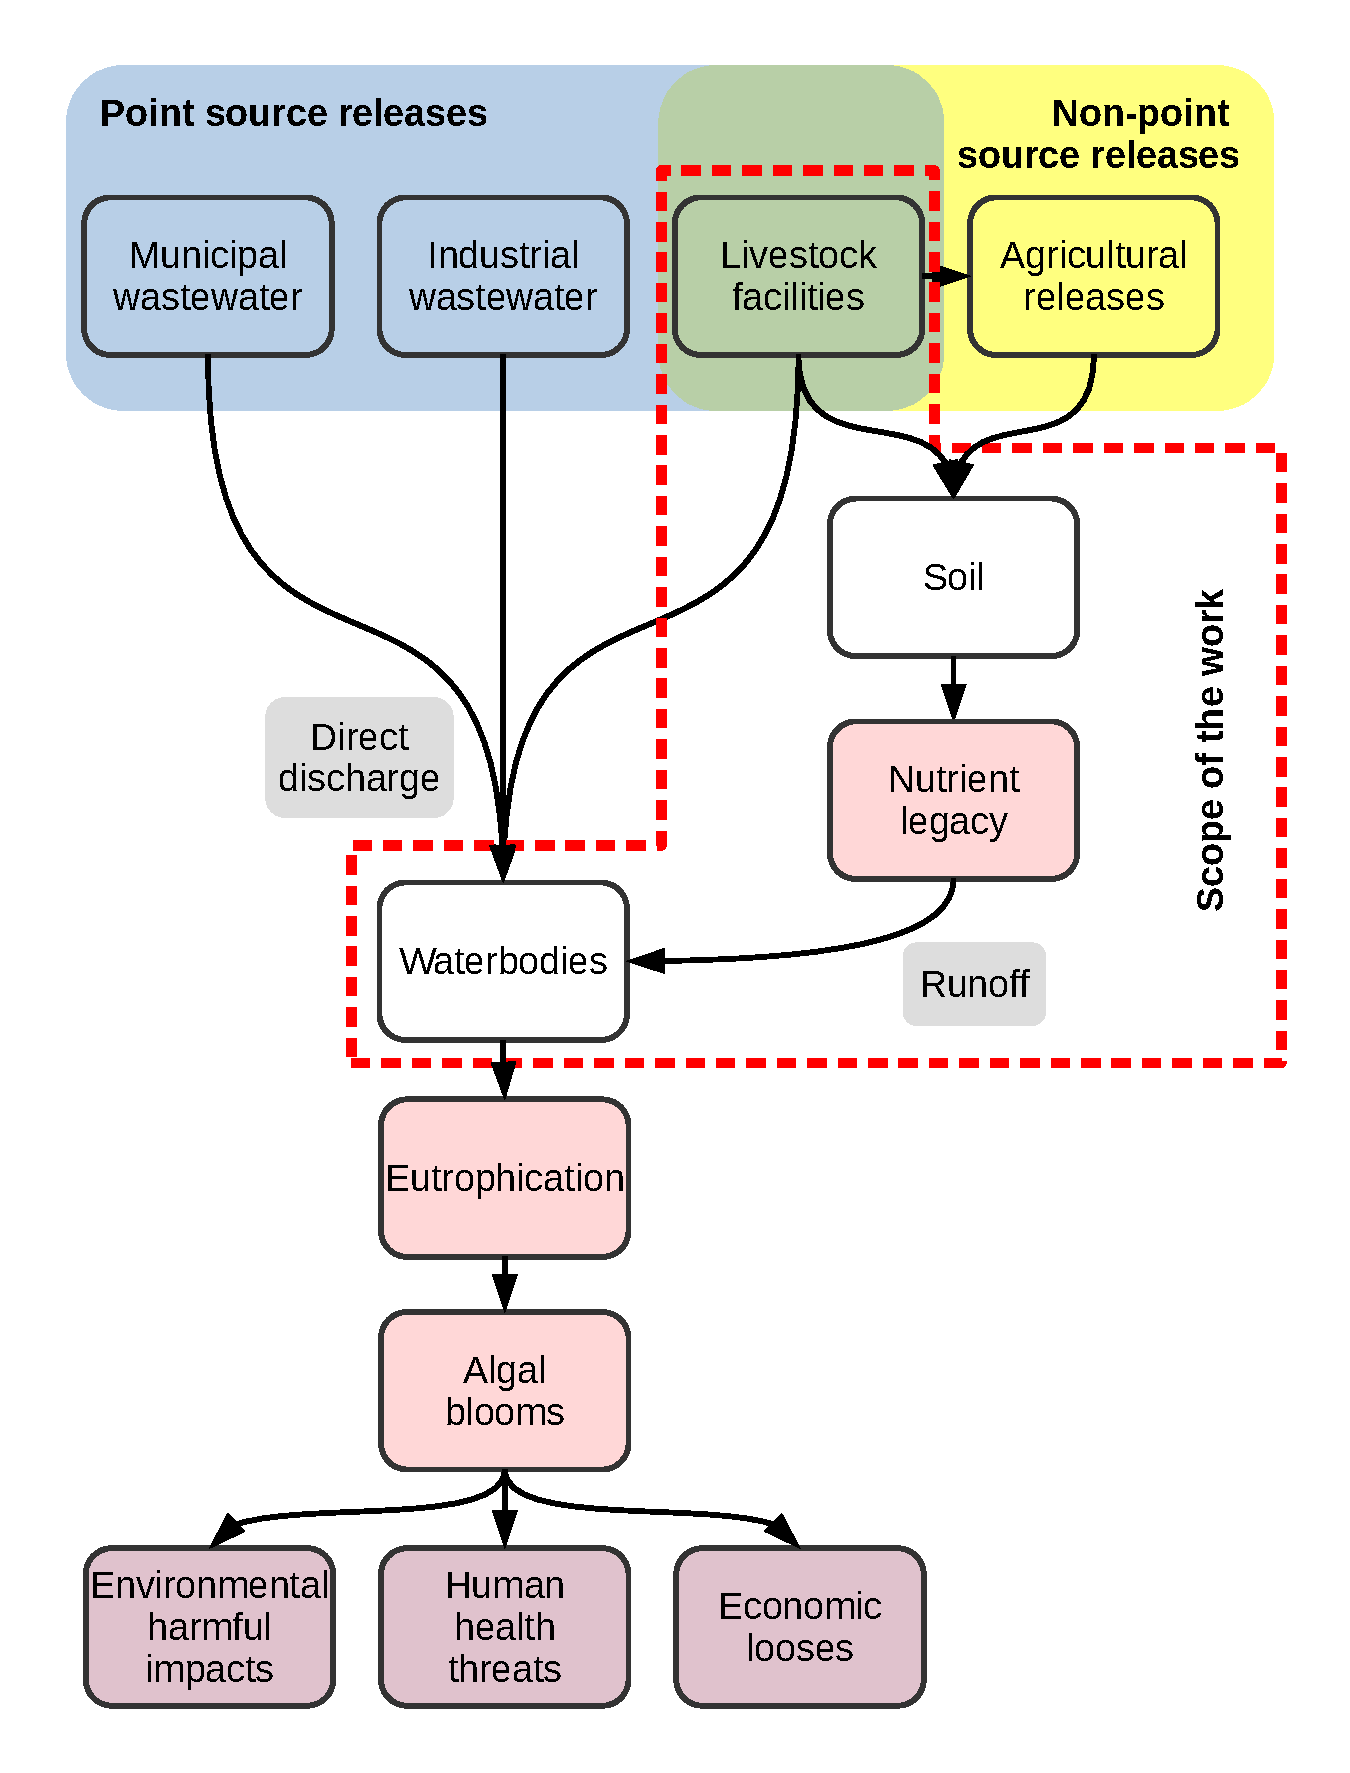
\includegraphics[width=0.85\linewidth, trim={1cm 1cm 1cm 1cm},clip]{gfx/Chapter1/IntroFig1.pdf} 
	\caption{Main flows of nutrients released by anthropogenic activities.}
	\label{fig:Ch1NutrientsFlow}
\end{figure}

In addition to the environmental problems, the use of nutrients for food production also raises geopolitical concerns since phosphorus is one to the most sensitive elements to depletion. Phosphorus is a non-renewable material whose reserves are expeted to be depleted in the next 50 to 100 years. Moreover, no substitute material is currently known \citep{cordell2009story}. Conversely, synthetic nitrogen can be produced using the atmospheric N\textsubscript{2} as raw material through the Haber-Bosh process. However, nowadays this process relies on non-renewable energy sources, and therefore the production of synthetic nitrogen--based fertilizers is dependent on non-renewable resources as well.

Considering the two challenges described, i.e., nutrient pollution of waterbodies as a consequence of agricultural and farming activities, and the current dependency on non-renewable resources for the production of synthetic fertilizers, nutrient recovery and recycling is not only a desirable but also a necessary approach to develop a sustainable agricultural paradigm and ensure the global food security.

Attending to the nutrient releases from intensive livestock farming facilities, known as concentrated animal feeding operations (CAFOs)\footnote{CAFO is a regulatory term defined by the U.S. Environmental Protection Agency for large facilities where animals are kept and raised in confined situations \citep{animal_unit_definition}. This term is used in this dissertation to denote the intensive livestock farming facilities studied.}, several manure management techniques are currently used. The land application of manure is a common technique that allows the recycling of nutrients as fertilizers for crops \citep{Kellog2010}. However, the increase of intensive livestock farming generates vast amounts of waste generated by CAFOs, e.g., each adult cow generates between 28 and 39 kg of manure per day, and each adult pig generates around 11.5 kg of manure per day \citep{USDAHandbook}. Manure processing is commonly based on the separation of liquid and solid phases. The liquid phase can be treated in anaerobic and/or aerobic lagoons for organic matter and pathogens removal, as well as odor control \citep{tilley2014compendium}. The obtained liquid effluent can be used for irrigation and nutrient supplementation of crops. The solid phase can be composted for the degradation of organic matter and pathogens removal, resulting in a solid material called compost with a larger amount of nitrogen and phosphorus available for plants, which is result of the mineralization of nutrients previously contained in organic compounds. Since compost is also a good source of organic matter for crops, it is a valuable material suitable for sale \citep{tilley2014compendium}. However, both materials, the liquid effluent obtained from the lagoons and compost, are too bulky to be economically transported to nutrient deficient locations \citep{burns2002phosphorus}. As a result, livestock waste is usually spread in the surroundings of livestock facilities, at a detrimental cost of environment. This result in the gradual build-up of nutrients in soils, which might lead the harmful environmental impacts previously described.

%Therefore, the implementation of processes for the recovery of phosphorus and nitrogen at CAFOs is a
A promising alternative for abating nutrient releases and reducing the environmental footprint of livestock industry is the implementation of processes for the recovery of phosphorus and nitrogen at CAFOs. At the time, that valuable nutrient-rich materials are obtained for the redistribution of phosphorus and nitrogen to nutrient-deficient areas. There exist a number of processes for nutrient recovery from livestock waste, which can be differentiated into those technologies oriented to phosphorus recovery, including struvite precipitation, calcium-based precipitates production, coagulation-flocculation, electrochemical processes, and systems based on solid-liquid
%phases
separation; and processes focused on nitrogen recovery, such as stripping, membrane separation, waste drying coupled with ammonia scrubbing, and
%phases
solid-liquid
separation processes. We note that anaerobic digestion is an additional process that can be integrated for manure treatment if the generation of biomethane is pursued, and for increasing the amount of recoverable nutrients through the partial mineralization of nutrients contained in organic compounds. It must be noted that only phosphorus and nitrogen in inorganic compounds can be taken by plants, and therefore the recovery of inorganic nutrients will be the target of the processes studied in this thesis.

The multiple processes for the recovery of phosphorus and nitrogen from livestock waste differ in aspects such as recovery efficiency, processing capacity, capital and operating costs, and products obtained. Therefore, a detailed analysis of each CAFO must be performed in order to select the optimal nutrient recovery system attending to type factors such as the type and amount of waste to be processed, the environmental vulnerability to eutrophication of each region, the current or potential installation of anaerobic digestion systems, etc. Additionally, in the decision-making process these factors have to be prioritized, i.e., sorted by relevance, to select the most suitable nutrient recovery system for each particular facility. As example,
%in regions with a low risk of eutrophication, more economical processes for nutrient recovery could be installed in even though their recovery efficiency may be lower than other alternatives. 
more economical processes for nutrient recovery, whose recovery efficiencies are typically lower, could be installed in regions with a low risk of eutrophication.
Conversely, regions at severe eutrophication risk require highly efficient nutrient recovery systems that may incur in larger investment and operating expenses. In order to perform a systematic evaluation of CAFOs and their context, we introduce a multi-criteria decision analysis (MCDA) framework integrating geospatial environmental data
%regarding
on eutrophication risk at the subbasin level and
%data from the 
techno-economic
%analysis
information of the studied processes. 

Attending to the regulatory aspect, nowadays most of the efforts for abating of nutrient releases into the environment and mitigating the eutrophication of waterbodies are focused on the limitation of fertilizer application in croplands. The application of fertilizer and manure for nitrogen supplementation in the European Union (EU) is currently regulated by the Nitrates Directive (91/676/EEC) \citep{GRIZZETTI2021102281}. Regarding the limitations for phosphorus application, these are defined at national level. Several European countries have implemented phosphorus application standards based on the different crops and materials used as fertilizers,
%. Generally, phosphorus application limits are
being generally more restrictive in Northwestern Europe \citep{amery2014agricultural}. 

In sum, it can be observed that nutrient application is limited either in the form of synthetic fertilizers or manure application. However, at present there is a lack of regulation regarding livestock waste treatment \citep{Piot_Lepetit2012}. In this regard, new efforts to promote the production and adoption of bio-fertilizers obtained from organic waste are being performed through the development of the "Integrated Nutrient Management Plan" (INMAP), which is part of the EU Farm-to-Fork strategy and part of the Circular Economy Action Plan. INMAP should propose actions to promote the recovery and recycling of nutrients, as well as the development of markets for recovered nutrients \citep{ESSP2021, CircularEconomyActionPlan}. In this regard, a new regulation for fertilizer products has been released in 2019 (EU 2019/1009), moving struvite and other biofertilizers from the category of waste to fertilizers, establishing a regulatory framework for their use and trade.

In the United States, CAFOs are regulated under the Clean Water Act as point source waste discharge. This regulation sets the need of permits for discharging pollutants to water, called National Pollutant Discharge Elimination System (NPDES) permits, including the release of nitrogen of phosphorus. This permit must include the necessary provisions for avoiding the harmful effects of the discharges on water and human health \citep{NPDE_basics}. The development and implementation of a Nutrient Management Plan (NMP) is a required element to get a NPDES permit. This document must identify the management practices to be implemented at the CAFO to protect natural resources from nutrient pollution. Land spreading of manure can also be regulated by the NPDES permits, establishing soil nutrient concentration limits and the yearly schedule for manure application. However, no specific methods or processes are defined under federal regulation \citep{NPDESforCAFO}. Regarding the use of the recovered nutrients, products obtained from nutrient recovery processes could be classified as waste ny the Clean Water Act, preventing the application of these materials on croplands \citep{NACWA503}. However, U.S. Environmental Protection Agency (US EPA) determined that, although these products could not be directly applied to land under the current regulation, they can be sold as a commodity to be outside of the Clean Water Act restrictions coverage. Moreover, US EPA acknowledges that highly refined and primarily inorganic products (such as struvite) could be outside of the scope of these restrictions \citep{CNP503}. However, further regulation is needed for defining the products obtained from nutrient recovery processes and to clearly state the conditions for their use as fertilizers on croplands.

Considering the previously described aspects, we note that the regulation of the products obtained from nutrient recovery systems is not totally developed yet, although important efforts are being performed in order to set a comprehensive regulatory framework for the recycling of phosphorus and nitrogen. Furthermore, no regulation regarding the implementation of nutrient recovery processes has been developed either in the EU and the US. However, both regions have developed programs to study and promote the implementation of other technologies for the treatment of livestock waste, specially the deployment of anaerobic digestion systems. These programs could be a guideline for the development of nutrient recovery plans at CAFOs. In this regard, we have studied the impact of the implementation of nutrient recovery systems in the economy of CAFOs, either considering the deployment of standalone nutrient recovery processes or integrated with anaerobic digestion for the production of electricity. Moreover, incentive policies have been analyzed to minimize the negative impact of nutrient recovery on CAFOs economy using the Great LAkes area as case study. In addition, the fair distribution of monetary resources when limited budget is available has been studied using the Nash allocation scheme. 

An overview of the main topics studied in this thesis can be observed in Figure \ref{fig:Ch1WorkThesis}. This work pretends to analyze strategies for promoting effective nutrient recycling addressing studies on the technical, environmental and economic dimensions involved, pursuing the development of sustainable food production paradigm.

\begin{figure}[h]
	\centering
	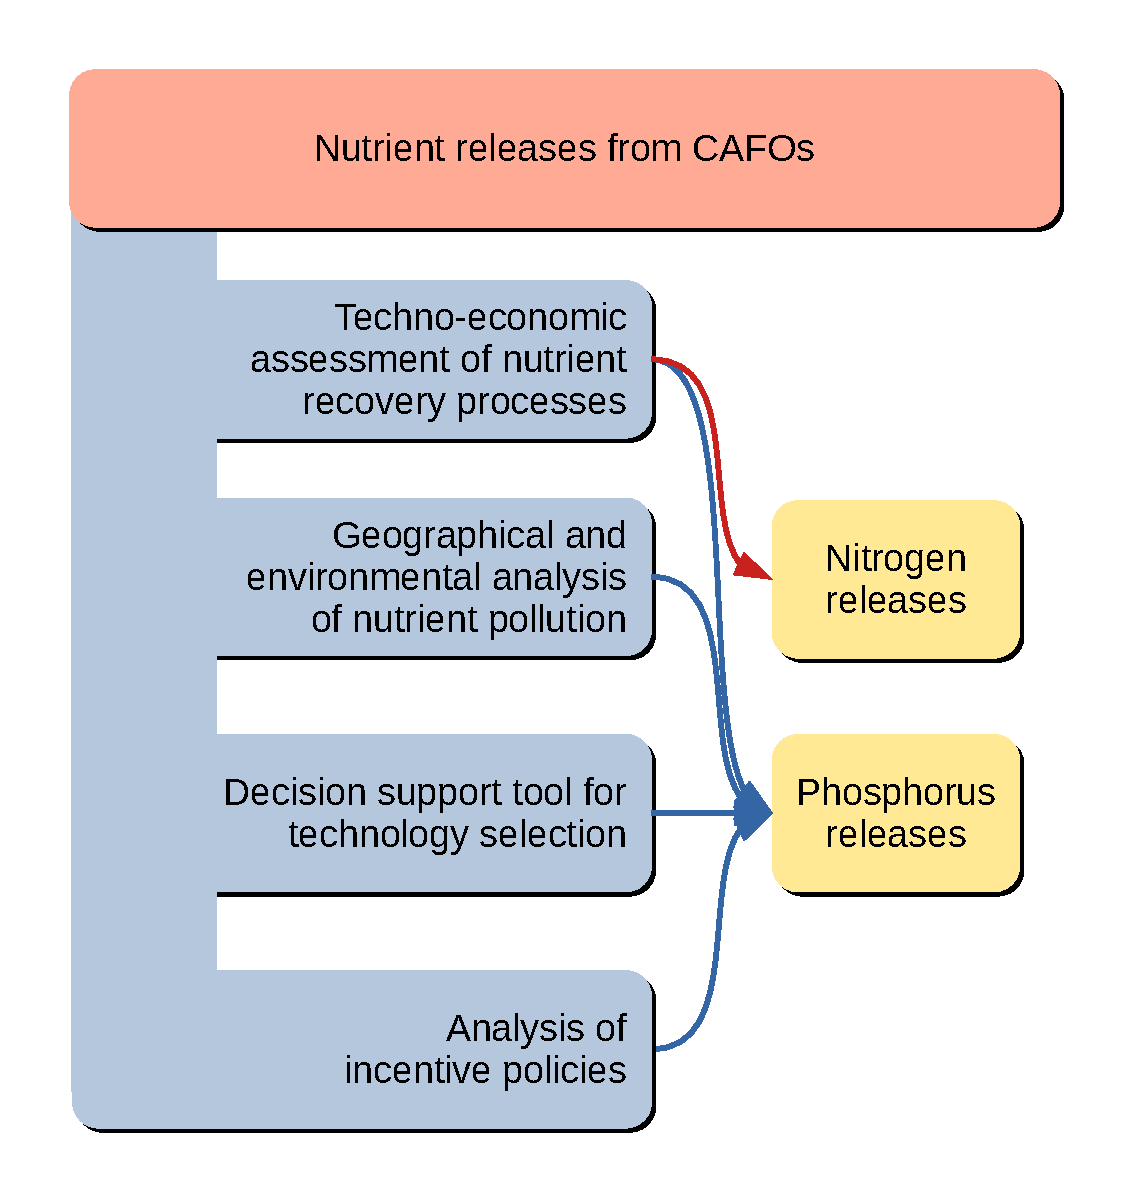
\includegraphics[width=0.7\linewidth, trim={1cm 1cm 1cm 1cm},clip]{gfx/Chapter1/IntroFig2.pdf} 
	\caption{Main topics covered in this work.}
	\label{fig:Ch1WorkThesis}
\end{figure}. 


%\section{Scope and objectives of the thesis}
%This thesis seeks to promote the recovery and recycling of nutrients contained in livestock waste by identifying the most appropriate technologies for phosphorus and nitrogen recovery at cattle and swine CAFOs, assessing the potential nutrient releases abatement that could be achieved by the deployment of these systems and analyzing incentive policies for their effective implementation at livestock facilities. Moreover, we introduce a systematic framework for evaluating and selecting the most suitable nutrient recovery system at CAFOs considering geospatial environmental vulnerability to nutrient pollution. 
%\paragraph{Objective I:} To perform a review of the state-of-the-art of the processes for phosphorus and nitrogen recovery from livestock waste, identifying those processes whose implementation at CAFOs is feasible from a techno-economic perspective.
%\paragraph{Objective II:} To identify environmental indicators for nutrient pollution, and use  them to  assess the potential for the abatement of phosphorus releases by deploying the processes previously selected at livestock facilities at subbasin spatial resolution.
%\paragraph{Objective III:} To develop a decision-support system for the evaluation and selection of nutrient recovery systems at livestock facilities integrating techno-economic data of the nutrient recovery technologies and environmental vulnerability to nutrient pollution information determined through a tailored geographic information system (GIS) in order to select  the most suitable system for each particular livestock facility.
%\paragraph{Objective IV:} To design and analyze potential incentive policies for the deployment of phosphorus recovery technologies at livestock facilities, as well as to study the fair allocation of limited monetary resources.

\section{Approaches for processes modeling}
Process modeling, defined as the mathematical modeling and simulation of systems, falls under the scope of Process System Engineering (PSE) discipline. These systems include physical, chemical, and/or biological operations. Process modeling forms the foundation for other activities involved in the scope of PSE, including process design, optimal scheduling and planning of the systems operations, and process control \citep{STEPHANOPOULOS20114272}.

Different modeling techniques have been developed to mathematically describe and represent systems from different domains, including but not limited to the chemical, biochemical, agrochemical, food, and pharmaceutical domains of engineering \citep{PISTIKOPOULOS2021107252}. An overview of the main modeling techniques is shown in the next sections based on the classification proposed by \citet{MARTIN201216}.

\subsection{Short-cut methods}
These type models are the most basic approach to process modeling. They are based on mass, energy, and momentum balances, and can be embedded in other models, such as supply chain models.

\subsection{Rules of thumb}
This approach is based on industrial operational data. It provides typical ranges for operating and design values, reflecting the actual parameters of the systems modeled. However, the use of these models is constrained by the availability of data. Compendiums of rules of thumb for different systems can be found in \citet{couper2005chemical, hall2012rules, sadhukhan2014biorefineries}.

\subsection{Dimensionless analysis}
This methodology is based on dimensionless groups that describe the performance of a particular system. These models are able to capture the physical meaning of the modeled processes, and they are specially useful to capture scale-up and scale-down issues \citep{szirtes2007applied}.

\subsection{Mechanistic models}
This approach relies on first principles for systems modeling, as short-cut models. However, mechanistic models rely in more detailed first principles such as the underlying chemistry, physics or biology that governs the behavior of a particular system. Chemical \citep{loeppert1995chemical} and phase \citep{brignole2013phase} equilibrium models, kinetic models \citep{buzzi2009kinetic}, population balances \citep{ramkrishna2000population}, and computer fluid dynamics (CFD) \citep{anderson1995computational} fall under this category.

\subsection{Surrogate models}
These models aim at developed simplified models from data obtained from rigorous mechanistic models. This approach is widely used for embedding system models into other applications such as process control or supply chain design. Surrogate models building has been systematized into four steps, i.e., design of experiments (DOE), running the rigorous models at the sampling points designated by the DOE, construction of the surrogate model, and validation of the model obtained \citep{queipo2005surrogate}.

Polynomial regression models, in which the relationship between the variables is expressed using a polynomial function, are one of the most basic types of surrogate models. In the case of polynomial regression models involving multiple variables, the optimal variables to be addressed within the pool of variables considered can be determined by using machine learning-based tools such as ALAMO \citep{wilson2017alamo}, ensuring an optimal trade-off between model accuracy and complexity. Other types of surrogate models are Kriging models, which estimate the relationship between variables as a sum of a linear model and a a stochastic Gaussian function representing the fluctuations of data \citep{quirante2015rigorous}, and artificial neural networks (ANN), which are based on  generating an input signal as the summation of all the
weighted inputs, which is through nodes containing a transfer function. Nodes are connected by edges with assigned weights that adjust the signals transmitted between nodes. Nodes are structured in layers, in a way that nodes receive signals from nodes of the preceding layer, and if the output of the node is above a threshold value defined by the transfer function, sends the output signal to the next layer \citep{himmelblau2000applications}.

\subsection{Experimental correlations}
As the surrogate models, experimental correlations are models built using data of the systems represented, but converserly to those one, experimental correlations are built using data  from experimental results. Similarly to the rules of thumb, the accuracy of these models is limited by the availability of data, and they are only applicable to the range of operating conditions of the data used for constructing the model.

\section{Approaches for decision-support systems}
Decision-making activities require to analyze multiple relevant criteria for each course of action. Since criteria often conflict each other, each decision-making process requires the balancing of criteria, prioritizing some criteria over other through the use of some criteria weighting scheme. This procedure requires managing a vast amount of information of conflicting nature, leading to a complex decision-making process. Therefore, different approaches generally called multiple-criteria decision analysis (MCDA) have been developed to explicitly structure and solve decision problems. MDCA aim is to integrate criteria assessment with value judgment to analyze and compare the different available alternatives, identifying the best solution for the decision-making context studied. However, it must be highlighted that a certain grade of subjectivity might exist is several steps of MCDA, such as the choice of the set of criteria that are considered relevant for a particular problem. Therefore, the solution proposed by any MCDA approach must be analyzed considering the assumptions made for building the problem. As a result, MCDA seeks to structure problems with multiple conflicting criteria, and providing justifiable and explainable solutions to guide decision-makers facing such problems. The solution of a multiple-criteria decision-making problem can defined as a unique solution representing the most suitable alternative from the set of potential alternatives for a particular decision-making context, or a subset of satisfactory alternatives \citep{belton2002multiple}.

A MCDA problem can be articulated in different stages, starting with the problem definition and structuring. At this stage, the goals, constraints, and stakeholders comprising the problem are defined, as well as the different solution alternatives. Based on this information, a model can be built for the assessment and comparison of alternatives. This stage includes the definition of the relevant criteria used for alternatives comparison, their relative priority, and the criteria evaluation system. Finally, the information retrieved by the model can be used for making informed decisions.

Multi-criteria decision-making problems can be divided into Multi-Attribute Decision Analysis (MADA), which are discrete choice problems where the number of alternatives is finite, and Multi-Objective Decision Analysis (MODA), that are mathematical programming problems that consider infinite number of alternatives, as shown in Figure \ref{fig:Ch1MCDA}. However, we note mathematical programming techniques are not limited to formulating and solving problems with infinite alternatives, but they can also be used for dealing with discrete decision-making problems \citep{giove2009decision}. 

\begin{figure}[h]
	\centering
	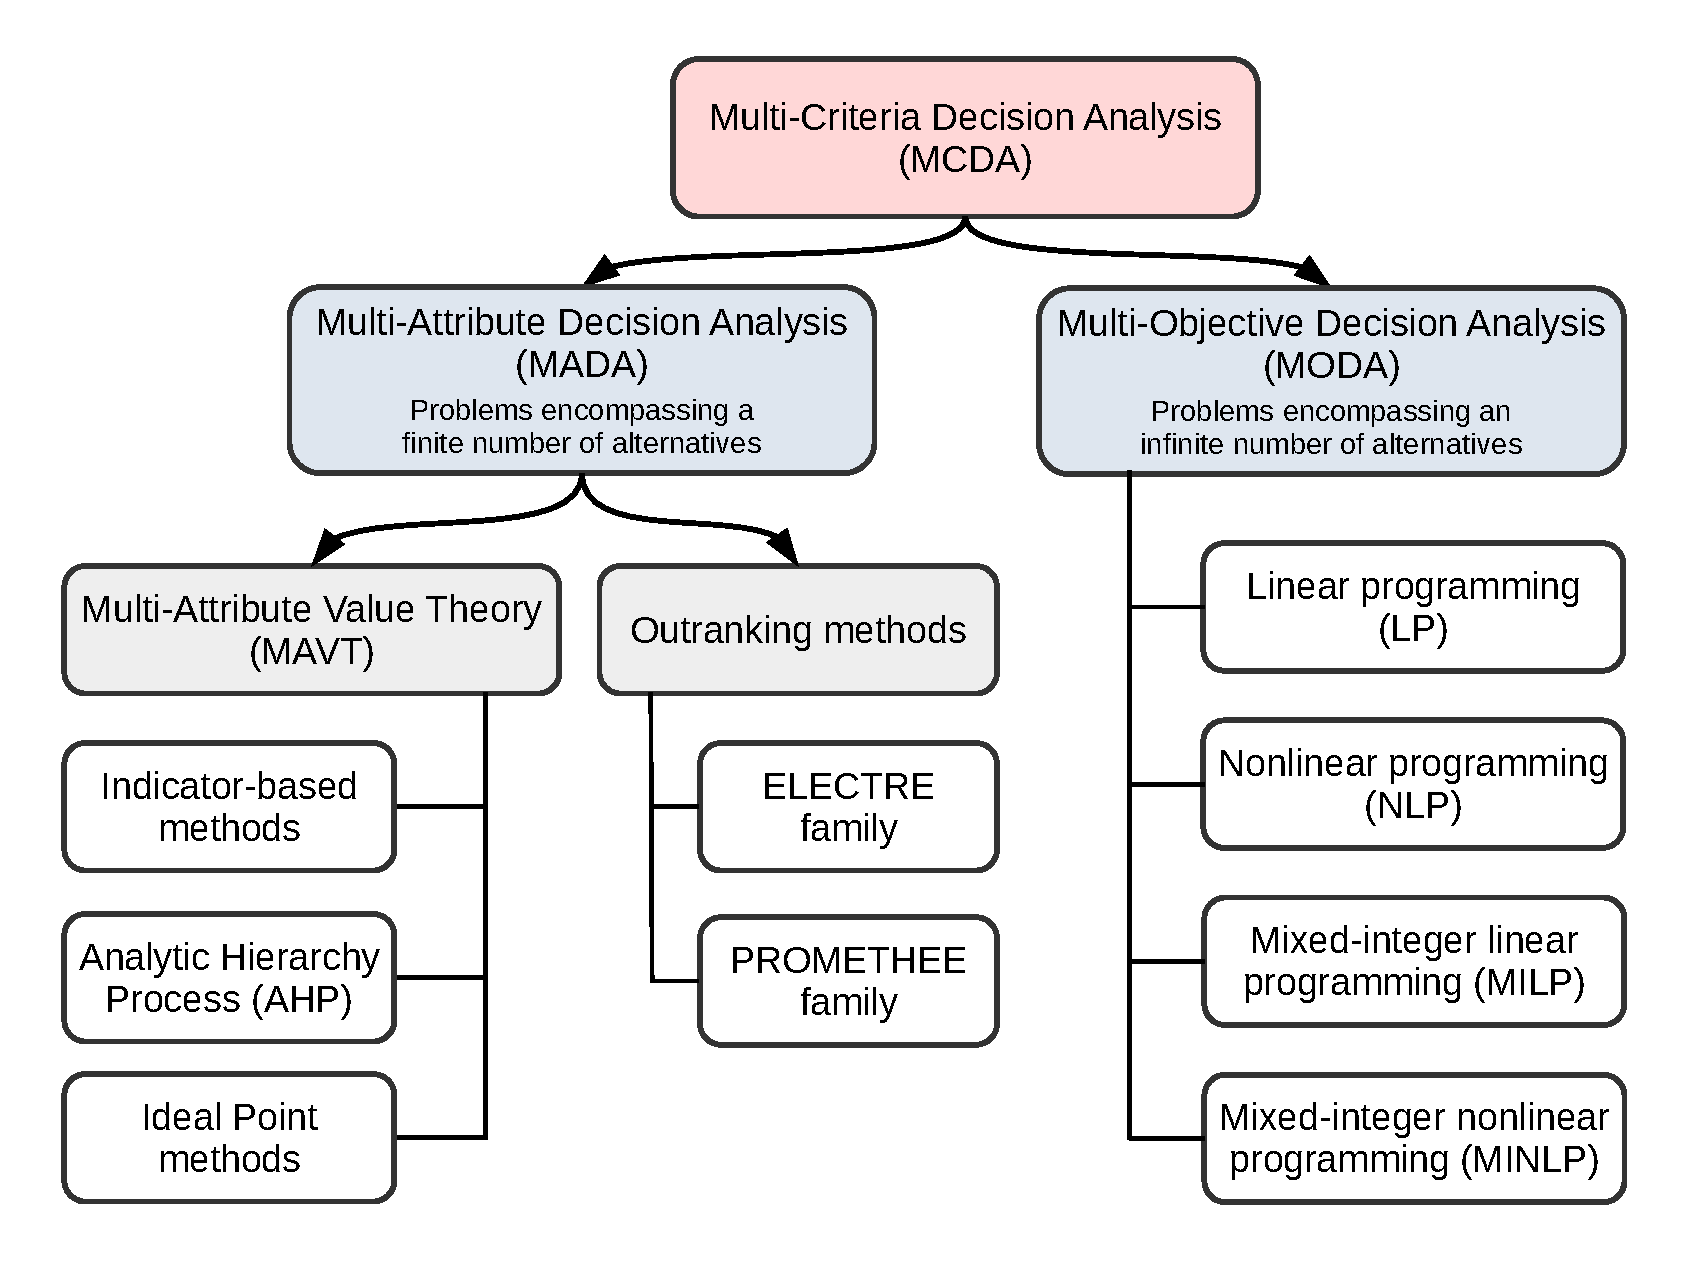
\includegraphics[width=1\linewidth, trim={1cm 1cm 1cm 1cm},clip]{gfx/Chapter1/IntroMCDA.pdf} 
	\caption{Classification of MCDA methods.}
	\label{fig:Ch1MCDA}
\end{figure}

\subsection{Multi-Attribute Decision Analysis (MADA)}

In the case of problems consisting of a finite number of alternatives, the suitability of each alternative to the problem given can be measured through its performance according to the multiple criteria considered. A large number of MCDA approaches have been (and are currently being) developed for discrete choice problems, including methods based on value functions (Multi-Attribute Value Theory methods, MAVT) and outranking methods.

\subsubsection{Multi-Attribute Value Theory (MAVT)}
\paragraph{Indicator-based methods}
Multi-Attribute Value Theory (MAVT) approaches are based on an indicator-based methodology is used for alternatives comparison. The relevant criteria considered in the decision-making process are a normalized to a common scale to allow criteria comparison using a utility or value function. A number of utility functions have been proposed in the literature, including standardization, min-max, and target utility functions \citep{HandbookCompositeIndicators}. 
The normalized criteria 
%are weighted to set the relative importance of each criterion, prioritizing some criteria over others. In the last step, weighted criteria 
are weighted and aggregated to build a composite index, prioritizing some criteria over others. Different aggregation schemes denote different degrees of compensability between indicators, i.e. a deficit in one criteria can be fully, partially, or not compensated by a surplus in other criteria \citep{MarcoCinelli2020}. Additive weighting aggregation is a full compensatory method, while geometric and  harmonic aggregation methods are partial  compensation schemes. Other aggregation schemes include geometric averaging, which is a non-compensatory method, and the Choquet integral \citep{marichal2000determination}. The composite index obtained is a single numerical value that can be used to score and rank the proposed alternatives based on their suitability to the criteria considered. 

%Uncertainty can be addressed with MAVT methods using different techniques, such as sensitivity analysis, bayesian approaches, and fuzzy set theory methods. 
A major source of uncertainty in indicator-based methods is the value of criteria weights. This can be addressed using the stochastic multi-criteria acceptability analysis (SMAA) method. SMAA is a sensitivity analysis method that address the uncertainty of criteria weights value exploring the feasible space of weights through the Monte Carlo method. Details about the SMAA approach can be found in \citet{tervonen_implementing_2007}.

%In this thesis, and indicator-based methodology has been used to assess and select phosphorus recovery technologies based on technical, environmental, and economic criteria combined in a composite index.

%Another MAVT approaches include Analytic Hierarchy Process (AHP) and the Ideal Point Methods. 
\paragraph{Analytic Hierarchy Process (AHP)}
Analytic Hierarchy Process (AHP) decomposes the decision problem in multiple simpler sub-problems. These sub-problems are hierarchized are independently analyzed. These sub-problems are solved through the pairwise comparison of the alternatives, obtaing numerical indexes that can be used to compare their performance. Finally a numerical weight (priority) is assigned to each element of the hierarchy, and they are used for aggregating the indexes obtained by each alternative in a final numerical value that can be used to score the overall performance of each alternative accordingly to the set of criteria considered \citep{saaty2000fundamentals}. 

\paragraph{Ideal Point methods}
Ideal Point methods set an optimal solution, that represent a utopia point where all criteria values are optimal. The performance of each alternative is evaluated through a composite index, that can be constructed using the techniques previously described. The alternatives are ranked based on their relative distance relative to the optimal solution. One of the most Ideal Point methods is TOPSIS \citep{hwang1995multi}.



%common scale to allow each criteria to be compared with the others.
%such as ELECTRE or PROMETHEE, analytic hierarchy process (AHP), fuzzy models, and indicator-based approaches, among others. In this thesis, and indicator-based methodology has been used to assess and select phosphorus recovery technologies based on technical, environmental, and economic criteria combined in a composite index. The construction of this composite index is composed of three steps: criteria normalization, weighting, and aggregation. Since each criteria has a different range of potential values, they must be normalized to a common scale to allow each criteria to be compared with the others. To account for robustness and resiliency of the solutions obtained, different normalization techniques have been studied. The normalized criteria are weighted to set the relative importance of each criterion, prioritizing some criteria over others. In order to avoid the risk of biasing the decision-making procedure setting arbitrary
%values for the weighting, a stochastic multi-criteria acceptability analysis (SMAA) is used to explore the weights space through the Monte Carlo method. Details about the SMAA approach can be found in \citet{tervonen_implementing_2007}. Finally, weighted criteria are aggregated to build the composite index. Different aggregation schemes denote different degrees of compensability between indicators, i.e. a deficit in one criteria can be fully, partially, or not compensated by a surplus in other criteria \citep{MarcoCinelli2020}.  Similarly to the normalization stage, different aggregation methods, including one full compensation and two partial compensation schemes are evaluated to achieve a robust solution.

\subsubsection{Outranking methods}
Outranking methods are based on the pairwise comparison of the alternatives for each criterion considered, determining the preferred alternative for each of the criteria. Preference information about all criteria is aggregated to establish evidence for selecting one alternative over another. These methods indicate the dominance of one alternative over another, but they do not quantify the performance gap between the alternatives compared \citep{giove2009decision}. Some of the most popular outranking methods are ELECTRE I \citep{roy1968classement}, II \citep{roy1973methode}, and III \citep{roy1978electre}, and PROMETHEE \citep{vincke1985preference}.

\subsubsection{Multi-Objective Decision Analysis (MODA)}

%Alternatively, p
Problems consisting of an infinite number of solutions require multi-objective mathematical programming (optimization) techniques to be solve. These problems are subjected to a number of equality and/or inequality constraints restricting the solutions that are feasible, and the multiple conflicting criteria are combined in an objective function. This objective function represents the improving level of the criteria, and it will be minimized or maximized for selecting the best solution that represents the optimal trade-off between the different conflicting criteria. In this thesis, this technique has been employed for selecting the operating conditions of processes for the recovery of nutrient, energy and biomethane from livestock waste, as it is shown in Chapters \ref{ch:PhosphorusTechs} and \ref{ch:BiogasUpgrading}. Other approach for solving multi-objective mathematical programming problems is to set a priory targets for different criteria, or combinations of criteria, that are considered satisfactory, obtaining the problem solution by minimizing the deviations from these goals. Mathematical programming problems can be also classified according to the use of linear or nonlinear equations, and continuous and/or discrete variables.

\paragraph{Linear programming (LP)}
Linear programming (LP) refers to those mathematical programming problems based on linear equations and continuous variables. A linear programming problem can be expressed as shown in Eq. \ref{eq:IntroEq1},  where $x$ is an n-vector, $A$ is a mxn matrix, $c$ is the n-vector of cost coefficients, and the right-hand side $b$ is an m-vector \citep{grossmann2021advanced}.

\begin{align}
	\min \quad & Z=c^{T}x \nonumber\\
	\textrm{s.t.} \quad & Ax=b \label{eq:IntroEq1}\\
	&x \geq 0  \nonumber  
\end{align}

The two most widely used methods to solve LP problems are the Simplex algorithm \citep{murty1983linear} and interior-point methods \citep{POTRA2000281}. The Simplex method is more efficient for solving problems with thousands of variables and constraints, while interior-point performs better on very large scale and sparse problems \citep{grossmann2021advanced}. These methods are implemented in solvers such as CPLEX \citep{cplex2009v12}, Gurobi \citep{gurobi}, or XPRESS \citep{xpress}.

\paragraph{Nonlinear programming (NLP)}
Nonlinear programming (NLP) refers to those mathematical programming problems containing nonlinear equations, either in the constrains or in the objective function, and continuous variables. A nonlinear programming problem can be expressed as shown in Eq.  \ref{eq:IntroEq2}, where $x$ is a n-vector, $f(x)$ is the objective function of the problem, $h(x)$ is the set of equality constraints and $g(x)$ is the set of inequality constraints \citep{floudas1995nonlinear}.

\begin{align}
\label{eq:IntroEq2}
\min \quad & f(x) \nonumber\\
\textrm{s.t.} \quad & h(x)=0\\
& g(x) \leq 0 \nonumber\\
&x \in X  \subseteq \Re^{n} \nonumber
\end{align}

Some of the most common algorithms to solve NLP problems are successive quadratic programming (SQP), reduced gradient algorithms, and interior point methods. 

SQP algorithms are based on the solution of quadratic programming subproblems. Each subproblem optimizes a quadratic model of the objective function subject to linearized constraints. In each of the iterations a search direction is determined reducing some merit function to ensure problem convergence \citep{gill2005snopt}. SNOPT is a solver based on this method \citep{gill2005snopt}.

Reduced gradient methods consider a linear approximation of the constraints and eliminate variables to reduce the dimension of the problem and apply the Newton’s method. In each of the iterations, the reduced gradient is calculated, the search direction is determined, and finally a line search is performed minimizing the objective function. MINOS \citep{murtagh1983minos} or CONOPT \citep{drud1985conopt} are solvers based on this algorithm.

Interior point methods reformulate the original NLP problem by means of slack variables to replaces inequalities by equalities, and the log-barrier function to handle the non-negativity of the x variables. The new problem is solve applying the Newton's method. IPOPT \cite{wachter2006implementation} and KNITRO \citep{waltz2004knitro} are solvers based on this approach

\paragraph{Mixed-integer linear programming (MILP)}
Mixed-integer linear programming (MILP) refers to those mathematical programming problems based on linear equations and containing discrete variables. A mixed-integer linear programming problem can be expressed as shown in Eq. \ref{eq:IntroEq3},where $x$ are continuous variables and $y$ are discrete variables. Typically, discrete variables are binary variables \citep{grossmann2021advanced}.

\begin{align}
		\min \quad & Z=a^{T}x + b^{T}y \nonumber\\
		\textrm{s.t.} \quad & Ax+By \leq d \label{eq:IntroEq3}\\
		& x \geq 0 \quad y \in \lbrace 0,1 \rbrace ^{m} \nonumber
\end{align}  

A number of methods have been proposed to solve MILP problems, including cutting planes, Benders decomposition, branch and bound search, and branch and cut methods.

Cutting planes consist of a sequence of LP problems in which different cutting planes are generated to cut-off the solution of the relaxed LP. They reduce the feasible region of the linear relaxation of the original problem excluding those solutions that are feasible in the linear relaxation but not in the original MILP problem. 

Benders decomposition is based on the generation of a lower and an upper bound of the solution of the MILP problem in each iteration. The upper bound is calculated from the primal problem, which correspond with the original problem where the binary variables have been fixed. Conversely, the lower bound is determined through a master problem, which is a LP problem derivated from the original problem by means of the duality theory. Branch and bound method structure the problem in form of a binary tree that includes all posible combinations of binary variables. The tree is explored by solving the relaxed versions of the original problem.  If the relaxation does not result in an integer solution (0 or 1), it is necessary to go deeper into the binery tree to explore further combinations of the binery variables. If the result obtained is an integer, the next step is to return to the previous subproblem to explore the alternative branch. However, diverse procedures have been developed to discard certain branches, avoiding the need of exploring the whole tree and reducing the problem \citep{floudas1995nonlinear}.

Branch and cut methods combine branch and bound methods with cutting planes targeting a tighter lower bound. In the different nodes, the relaxation of the problem is solved. If the solution is not integer, the relaxing problem is solved by adding cutting planes in order to strengthen the lower bound \citep{grossmann2021advanced}. Gurobi \citep{gurobi} and CPLEX \citep{cplex2009v12} are solvers based on this approach.

\paragraph{Mixed-integer nonlinear programming (MINLP)}
Mixed-integer nonlinear programming (MINLP) refers to those mathematical programming problems containing nonlinear equations and discrete variables, typically, binary variables. A mixed-integer nonlinear programming problem can be expressed as shown in Eq \ref{eq:IntroEq4}, where $x$ represents a vector of continuous variables, $y$ is the vector of binary variables, $h(x,y)$ and $g(x,y)$ denote the equality and inequality constraints respectively and, finally, $f(x)$ is the objective function \citep{grossmann2021advanced}.

\begin{align}
	\min \quad & f(x,y) \nonumber\\
	\textrm{s.t.} \quad & h(x,y)=0 \nonumber\\
	& g(x,y) \leq 0 \ref{eq:IntroEq4} \\
	& x \in X  \subseteq \Re^{n} \nonumber\\ 
	& y \in \lbrace 0,1 \rbrace ^{m} \nonumber
\end{align}  

Some algorithms for solving MINLP problems are the generalized Benders decomposition, outer approximation, and generalized cross decomposition. 

Generalized Benders decomposition (GBD) is based on the generation of a lower and an upper bound of the solution of the MINLP problem in each iteration. Similarly to the Benders decomposition, the upper bound is calculated from the primal problem, which correspond with the original problem where the binary variables have been fixed. The lower bound is determined through a master problem, which is a LP problem derivated from the original problem by means of the duality theory.  In addition, the master problem provides
information about the binary variables to be fixed in the next iteration \citep{floudas1995nonlinear}.

Outer approximation (OA) provides a lower and an upper bound in each iteration. As the previous case, the upper bound is calculated from the primal problem. The lower bound is calculate from a master problem obtained based on an outer approximation, i.e., a linearization of the nonlinear objective and constraints function is performed around the primal solution. Additionally, the master problem provides information about the binary variables to be fixed in the next iteration.

Generalized cross decomposition (GCD) is based on the generation of a primal problem that provides an upper bound of the solution and also Lagrange multipliers for the dual subproblem. The dual problem is used to determine the lower bound of the problem, and provides a vector of binary variables to be fixed in the primal problem. The solution of the primal and dual problems go through convergence tests. If any of these test fails, a master problem is solved, although the computational requirements of the this problem are higher. This procedure is repeated at each iteration of the algorithm \citep{floudas1995nonlinear}.

\section{Approaches for geospatial environmental assessment}
Human actions, from food production\citep{foster2007environmental} to cloud computing \citep{di2017can}, result in harmful impacts endangering and deteriorating the environment. The development of mitigation measures to reduce the environmental footprint of anthropogenic activities requires the previous understanding and quantification of the environmental impacts associated to each sector. This process, called environmental impact assessment (EIA), involves the analysis of multi-disciplinary information, including environmental, physical, geological, ecological, economic, and social data \citep{gharehbaghi2018gis}. Since EIA aims to evaluate the environmental impact of an activity on a particular geographical location, all these data have a common geographic component, becoming geospatial data.

Geospatial data can be managed and analyzed through specific systems denoted as geographic information system (GIS). GIS is a key tool for EIA that uses the geographic component of geospatial data as an integrative framework that provides the ability to analyze and map descriptive information of the locations studied. The geographic component of data is the key element of GIS systems, since the spatial (or spatio-temporal) location is used as a key to relate other descriptive information. From the perspective of EIA, this information can be analyzed, interpreted, and mapped to determine the vulnerability level of each location to a particular environmental threat, find relationships between human activities and environmental damages, measure the performance of mitigation and remediation processes, etc.

The combination of GIS, EIA, and methods for the analysis of multi-dimensional information, such as MCDA, provides tools for the development of sustainable strategies for the transition to a sustainable paradigm for human growth. In this regard, the development of a sustainable, reliable, and resilient water, energy and food nexus is a major issue for food security and environmental protection.

\section{Thesis outline}
This dissertation is structured in three parts. Part I is devoted to the study of phosphorus management and recovery, Part II address a techno-economic assessment of the technologies for nitrogen recovery, and Part III conduct a research for determining the best combination of units for biomethane production in order to integrate biogas production and nutrient recovery processes.

\subsection{Part I - Phosphorus management and recovery}
\paragraph{Chapter \ref{ch:PhosphorusTechs} - Technologies for phosphorus recovery.} This chapter performs a review of the main processes for phosphorus recovery from livestock waste, identifying the most promising processes to be deployed at CAFOs using a mixed-integer nonlinear programming model.

\paragraph{Chapter \ref{ch:Struvite} - Assessment of phosphorus recovery through struvite precipitation.} This chapter study the mitigation of phosphorus releases through the deployment of struvite precipitation systems in the watersheds of the contiguous Unites States. Specific surrogate models to predict the production of struvite and calcium precipitates from cattle leachate were developed based on a detailed and robust thermodynamic model. In addition, the variability in the organic waste composition is captured through a probability framework based on Monte Carlo method.

\paragraph{Chapter \ref{ch:Tool} - Geospatial environmental and techno-economic framework for sustainable phosphorus management at livestock facilities.} This chapter presents a decision support framework, COW2NUTRIENT (Cattle Organic Waste to NUTRIent and ENergy Technologies), for the assessment and selection of phosphorus recovery technologies at CAFOs based on environmental information on nutrient pollution and techno-economic criteria. This framework combines eutrophication risk data at subbasin level and the techno-economic assessment of six state-of-the-art phosphorus recovery processes in a multi-criteria decision analysis (MCDA) model. We aimed to provide a useful framework for the selection of the most suitable P recovery system for each particular CAFO, and for designing and evaluating effective GIS-based incentives and regulatory policies to control and mitigate nutrient pollution of waterbodies.

\paragraph{Chapter \ref{ch:Policies} - Analysis of incentive policies for phosphorus recovery.} This chapter conduct a research on the design and analysis of incentive policies using the COW2NUTRIENT framework for the implementation of phosphorus recovery technologies at CAFOs minimizing the negative impact in the economic performance of CAFOs. Moreover, the fair allocation of monetary resources when the available budget is limited is studied using the Nash allocation scheme.

\subsection{Part II - Nitrogen management and recovery}
\paragraph{Chapter \ref{ch:NitrogenTechs} - Multi-scale techno-economic assessment of nitrogen recovery systems for swine operations.} This chapter performs a review of the main processes for nitrogen recovery at intensive swine operations. A multi-scale techno-economic analysis is performed to estimate the capital and operating costs for different treatment capacities, identifying the most promising processes.

\subsection{Part III - Nitrogen management and recovery}
\paragraph{Chapter \ref{ch:BiogasUpgrading} - Optimal technology selection for the biogas upgrading to biomethane.} This chapter performs a systematic study of different biogas upgrading to biomethane processes in order to identify the optimal process attending to the particular characteristics of the biogas produced from livestock manure. Food waste and wastewater sludge are also included for comparison. We aimed to determine the optimal biomethane production processes for the potential combination of biomethane production and nutrient recovery processes into an integrated resources recovery facility.
%The case study demonstration consists of implementing and assessing the sustainable performance of nutrient and energy recovery at 2,217 CAFOs located in the U.S. Great Lakes area (i.e., Minnesota, Indiana, Ohio, Pennsylvania, Wisconsin, and Michigan).

%technic, economic, and environmental dimensions of nutrient recovery at CAFOs have been integrated in a decission support system 
\section*{Bibliography}
\addcontentsline{toc}{section}{Bibliography}
\printbibliography[heading=none]
\end{refsection}
%************************************************
\chapter{Objective}\label{ch:objectives}
%************************************************
%\begin{refsection}[referencesCh1]

%\section{Scope and objectives of the thesis}
\section{Scope and objectives of the thesis}
\section{Main objective}
This thesis seeks to promote the recovery and recycling of nutrients contained in livestock waste by identifying the most appropriate technologies for phosphorus and nitrogen recovery at cattle and swine CAFOs, assessing the potential nutrient releases abatement that could be achieved by the deployment of these systems and analyzing incentive policies for their effective implementation at livestock facilities. Moreover, we introduce a systematic framework for evaluating and selecting the most suitable nutrient recovery system at CAFOs considering geospatial environmental vulnerability to nutrient pollution. 

\section{Specific objectives}
\paragraph{Objective I:} To perform a review of the state-of-the-art of the processes for phosphorus and nitrogen recovery from livestock waste, identifying those processes whose implementation at CAFOs is feasible from a techno-economic perspective.
\paragraph{Objective II:} To identify environmental indicators for nutrient pollution, and use  them to  assess the potential for the abatement of phosphorus releases by deploying the processes previously selected at livestock facilities at subbasin spatial resolution.
\paragraph{Objective III:} To develop a decision-support system for the evaluation and selection of nutrient recovery systems at livestock facilities integrating techno-economic data of the nutrient recovery technologies and environmental vulnerability to nutrient pollution information determined through a tailored geographic information system (GIS) in order to select  the most suitable system for each particular livestock facility.
\paragraph{Objective IV:} To design and analyze potential incentive policies for the deployment of phosphorus recovery technologies at livestock facilities, as well as to study the fair allocation of limited monetary resources.

%\section*{Bibliography}
%\addcontentsline{toc}{section}{Bibliography}
%
%\printbibliography[heading=none]
%\end{refsection}

%\setcounter{page}{90}
% use \cleardoublepage here to avoid problems with pdfbookmark
\cleardoublepage
%\ctparttext{Complete introduction of Part I}
\part{Phosphorus management and recovery}\label{pt:Phosphorus}
%\cleardoublepage%*****************************************
\chapter{Technologies for phosphorus recovery}\label{ch:PhosphorusTechs}
%*****************************************
\begin{refsection}[referencesCh2]
\section*{Abstract}
A mixed-integer nonlinear programming strategy is proposed to design integrated facilities to simultaneously recover power and nutrients from organic waste. The facilities consider anaerobic digestion of different types of manure (cattle, pig, poultry, and sheep). The products from this step are biogas and a nutrient-rich effluent. The biogas produced is cleaned and used in a gas turbine to produce power while the hot flue gas obtained from combustion produces steam that is fed to a steam turbine to produce additional power. The nutrient-rich effluent is processed to recover the nutrients using different technologies that include filtration, coagulation, centrifugation, and struvite precipitation in stirred and fluidized bed reactors. This processing step provides a mechanism to prevent phosphorus or nitrogen release to the environment and to avoid the development of eutrophication processes. It is found that struvite production in fluidized beds is the technology of choice to recover nutrients from all manure sources. Furthermore, power production depends strongly on manure composition and exhibits high cost variability (from 4,000 €/kW in the case of poultry manure to 25,000 €/kW in the case of cattle and pig manure).

%\textbf{}
\bigskip
\textbf{Keywords:} Biogas; Digestate; Anaerobic digestion; Manure; Power production; Mathematical optimization

\newpage

\section*{Resumen}
Se propone una estrategia de programación mixta entera no lineal para diseñar instalaciones integradas de recuperación simultánea de energía y nutrientes contenidos en residuos orgánicos. Las instalaciones propuestas consideran la digestión anaeróbica de diferentes tipos de deyecciones ganaderas (vacuno, porcino, avícola y ovino). Los productos de este proceso son biogás y un efluente rico en nutrientes. El biogás producido es purificado y es utilizado en una turbina de gas para producir energía eléctrica, mientras que los gases de combustión calientes resultantes de la combustión se emplean en la generación de vapor que se alimenta a una turbina de vapor para producir energía adicional. El efluente rico en nutrientes se procesa para recuperar los nutrientes utilizando diferentes tecnologías que incluyen filtración, coagulación, centrifugación y precipitación de estruvita en reactores de mezcla completa y en reactores de lecho fluidizad. Este tratamiento proporciona un mecanismo para prevenir la liberación de fósforo o nitrógeno al medio ambiente y evitar el desarrollo de procesos de eutrofización. Se ha comprobado que la producción de estruvita en reactores de lecho fluidizado es la tecnología seleccionada para recuperar los nutrientes de todas las fuentes de estiércol. Además, la producción de energía depende en gran medida de la composición del estiércol y presenta una gran variabilidad de costes (desde 4.000 euros/kW en el caso del estiércol de aves de corral hasta 25.000 euros/kW en el caso del estiércol de vacuno y de cerdo).

\bigskip
\textbf{Palabras clave:} Biogás; Digestato; Digestión anaerobia; Deyecciones ganaderas; Producción de electricidad; Optimización matemproduccióntica


\newpage

\section{Introduction}
Countries across the globe generate large amounts of organic waste that include urban residues and sludge and manure from livestock activities. While many of these waste streams can be used as a source for power and chemical products, identifying suitable cost-effective technologies
is challenging. Anaerobic digestion (AD) is a promising technology to treat these residues to produce biogas, which can be used as a source for thermal energy and electrical power \citep{Leon} or chemicals \citep{hernandez2016optimal}. However, AD technologies also generate a nutrient-rich residual stream called digestate, that must be further processed to prevent waste and soil contamination. In particular, nutrient management is needed to prevent losses of phosphorous and nitrogen to surface and underground water bodies which leads to eutrophication processes \citep{Sampat2017, GarciaSerrano}. There are a number of technologies that can be used to process the digestate that range from simple mechanical separations such as filters \citep{gustafsson2008phosphate} and centrifugation units \citep{meixner2015effect} to chemical processing such as struvite precipitation \citep{bhuiyan2008phosphorus}. Recent studies have analyzed the production of highly concentrated nutrient products such as struvite \citep{lin2015phosphorus}. The variability in the recovered product quality, selling price, and production cost presents complex trade-offs for the optimal use of the digestate. Existing studies have only addressed the performance of various treatment mechanisms and lack a systematic design perspective that evaluates the performance of coupled biogas and nutrient recovery technologies \citep{drosg2015nutrient}. This is necessary, for instance, to assess economic performance of nutrient recovery in the face of strong variations in the digestate content obtained from AD \citep{AlSeadi2008}.

In this work we propose a systematic design framework to optimize the simultaneous production of energy from the biogas obtained by anaerobic digestion of cattle, sheep, poultry and pig manure, along with the recovery of nitrogen and phosphorous from the digestate. The proposed framework determines the optimal technology configuration, equipment sizing, and operational conditions for various compositions of manure and digestate and revenues for biogas, electricity, and fertilizer. 

The paper is organized as follows. In Section \ref{section:ProcessDescription} we present a brief description of the process and the flowsheet. In Section \ref{section:ModellingIssues} we focus on the modelling of the digestate processing technologies and costing. Section \ref{section:Results} presents the results for various feedstocks, and Section \ref{section:Conclusions} draws conclusions.

\section{Process description} \label{section:ProcessDescription}
The proposed process consists of four sections: biogas production, biogas purification (biogas generation), electrical power generation, and nutrient recovery from digestate. This is illustrated in Figure \ref{fig:Flowsheet}.

\begin{figure}[h!]
	\centering
	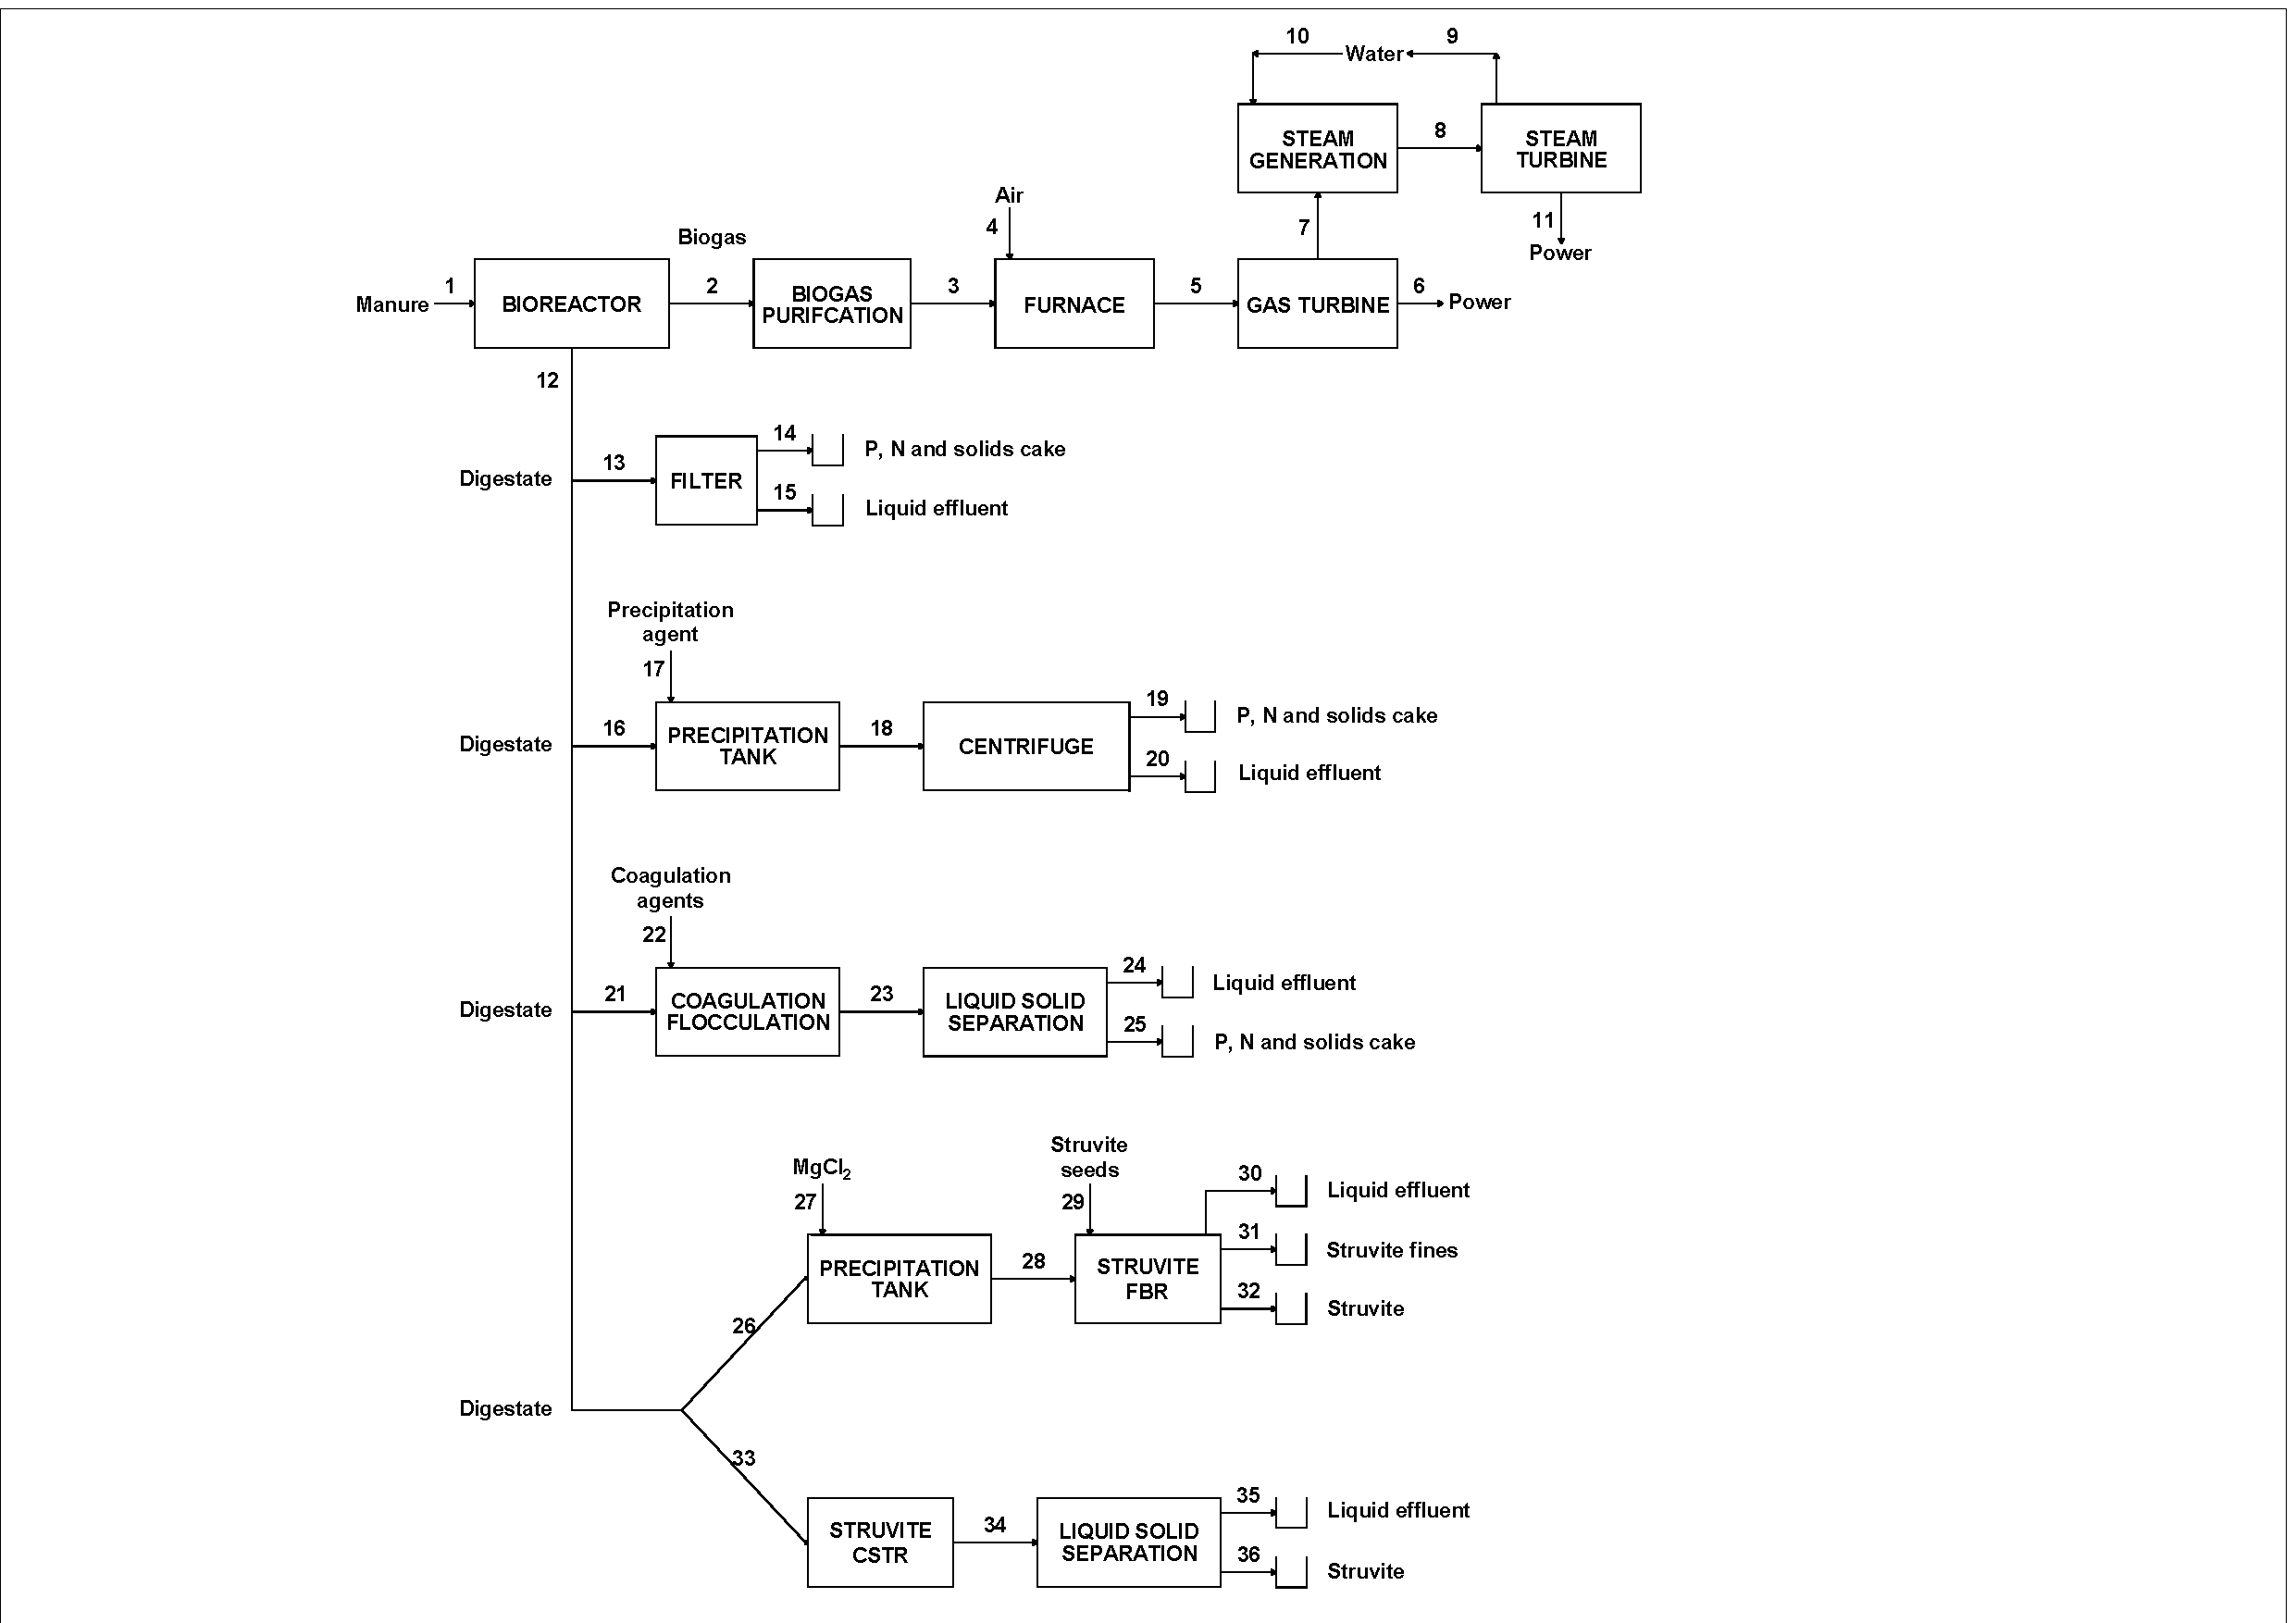
\includegraphics[width=1\linewidth, trim={6.5cm 0.1cm 11.5cm 0.3cm},clip]{gfx/Chapter2/superstructure3bloquesCOMPATIBILIDAD-Layout3.pdf} 
	\caption{Flowsheet for the production of power and fertilizers.}
	\label{fig:Flowsheet}
\end{figure}

The biomass together with water and nutrients (manure slurry) are fed to a bioreactor through stream 1, where the mixture is anaerobically digested to produce biogas and a decomposed substrate (digestate). The biogas, composed of methane, carbon dioxide, nitrogen, hydrogen sulfide, ammonia and moisture leaves the bioreactor through stream 2, and it is then sent to the purification section to remove H\textsubscript{2}S in a fixed-bed reactor and to eliminate CO\textsubscript{2} and traces of NH\textsubscript{3} in a second step by using a pressure swing adsorption (PSA) system. The purified biogas (stream 3) is used in a Brayton cycle, modelled as a furnace and an expansion, producing power. Air is fed via stream 4 and the exhaust gases (stream 7) are fed to a regenerative Rankine cycle, where it produces high pressure overheated steam extracted in stream 8. This overheated steam is fed to a steam turbine, where it is expanded to produce power. The exhaust steam from the turbine is recovered in stream 9 and reused in the Rankine cycle through stream 10. Between streams 9 and 10 hot flue gases from the gas turbine reheat and produced overheated steam from the recycled water \citep{Leon}.

The digestate is released from the digester through stream 12, and it can be processed through a number of technologies to remove nitrogen and phosphorous. We consider filtration, centrifugation, coagulation, and struvite production using either a fluidized bed reactor (FBR) or a continuous stirred tank reactor (CSTR). These technologies are described in detail in Section \ref{section:DigestateConditioning}.

Four manure types have been considered as raw material for the process: cattle, pig, poultry and sheep manure. Table \ref{table:techs_description} shows the composition and properties of each type of manure.

\begin{table}[]
	\centering
	\caption{Manure composition and properties \protect\citep{kowalski2013changes, Lorimor2004, AlSeadi2008, martins2009biogas}.}
	\label{table:techs_description}
	\resizebox{\columnwidth}{!}{
	\begin{tabular}{@{}ccccccccccccccc@{}}
		\toprule
		\multirow{2}{*}{\begin{tabular}[c]{@{}c@{}}Manure/\\ element\end{tabular}} & \multicolumn{2}{c}{\begin{tabular}[c]{@{}c@{}}Dry matter\\ (\% wt)\end{tabular}} & \multicolumn{2}{c}{\begin{tabular}[c]{@{}c@{}}N\\ (\% dry mass)\end{tabular}} & \multicolumn{2}{c}{\begin{tabular}[c]{@{}c@{}}P\\ (\% dry mass)\end{tabular}} & \multicolumn{2}{c}{\begin{tabular}[c]{@{}c@{}}K\\ (\% dry mass)\end{tabular}} & \multicolumn{2}{c}{\begin{tabular}[c]{@{}c@{}}VS\\ (\% dry mass)\end{tabular}} & \multicolumn{2}{c}{\begin{tabular}[c]{@{}c@{}}V\textsubscript{biogas}\\ $\left(\frac{\text{m\textsuperscript{3}\textsubscript{gas}}}{\text{kg\textsubscript{VS}}}\right)$\end{tabular}} & \multicolumn{2}{c}{\begin{tabular}[c]{@{}c@{}}Density\\ $\left(\frac{\text{kg}}{\text{m\textsuperscript{3}}}\right)$\end{tabular}} \\ \cmidrule(l){2-3} \cmidrule(l){4-5} \cmidrule(l){6-7} \cmidrule(l){8-9} \cmidrule(l){10-11} \cmidrule(l){12-13}
		& Max                                     & Min                                    & Max                                   & Min                                   & Max                                   & Min                                   & Max                                   & Min                                   & Max                                    & Min                                   & Max                                      & Min                                     &                                          &                                   \\ \midrule
		Cattle                                                                     & 10                                      & 2                                      & 8                                     & 4.7                                   & 1.3                                   & 0.8                                   & 10                                    & 3.3                                   & 0.8                                    & 0.8                                   & 0.3                                      & 0.2                                     & 1041.2                                   &                                   \\
		Pig                                                                        & 6                                       & 2                                      & 15                                    & 13                                    & 2.2                                   & 1.9                                   & 8.3                                   & 3.9                                   & 0.8                                    & 0.7                                   & 0.5                                      & 0.25                                    & 1000.0                                   &                                   \\
		Poultry                                                                    & 60                                      & 30                                     & 5.4                                   & 5.4                                   & 1.7                                   & 1.7                                   & 1.2                                   & 2.3                                   & 0.8                                    & 0.8                                   & 0.6                                      & 0.35                                    & 1009.2                                   &                                   \\
		Sheep                                                                      & 28                                      & 28                                     & 2.9                                   & 2.9                                   & 0.78                                  & 0.78                                  & 2.9                                   & 2.9                                   & 0.8                                    & 0.8                                   & 0.61                                     & 0.37                                    & 1009.2                                   &                                   \\ \bottomrule
	\end{tabular}
	}
\end{table}

\begin{table}[]
	\centering
	\caption{Set of components.}
	\label{table:SetComponents}
	\resizebox{\columnwidth}{!}{
		\begin{tabular}{@{}cccccccc@{}}
			\toprule
			\begin{tabular}[c]{@{}c@{}}Number of \\ component\end{tabular} & Component & \begin{tabular}[c]{@{}c@{}}Number of \\ component\end{tabular} & Component      & \begin{tabular}[c]{@{}c@{}}Number of \\ component\end{tabular} & Component      & \begin{tabular}[c]{@{}c@{}}Number of \\ component\end{tabular} & Component      \\ \midrule
			1                    & Wa        & 12                   & O              & 23                   & K\textsubscript{2}O            & 34                   & Cl             \\
			2                    & CO\textsubscript{2}       & 13                   & N              & 24                   & CaCO\textsubscript{3}          & 35                   & Struvite       \\
			3                    & CO        & 14                   & Norg           & 25                   & FeCl\textsubscript{3}          & 36                   & K-Struvite      \\
			4                    & O\textsubscript{2}        & 15                   & P              & 26                   & Antifoam       & 37                   & MgCl\textsubscript{2} (CSTR)     \\
			5                    & N\textsubscript{2}        & 16                   & K              & 27                   & Fe\textsubscript{2}(SO\textsubscript{4})\textsubscript{3}      & 38                   & NaOH (CSTR)      \\
			6                    & H\textsubscript{2}S      & 17                   & S              & 28                   & Al\textsubscript{2}(SO\textsubscript{4})\textsubscript{3}      & 39                   & Mg (CSTR)        \\
			7                    & NH\textsubscript{3}       & 18                   & Rest           & 29                   & AlCl\textsubscript{3}          & 40                   & Cl (CSTR)        \\
			8                    & CH\textsubscript{4}       & 19                   & Cattle slurry  & 30                   & MgCl\textsubscript{2}          & 41                   & Struvite (CSTR)  \\
			9                    & SO\textsubscript{2}       & 20                   & Pig slurry     & 31                   & NaOH           & 42                   & K-Struvite (CSTR) \\
			10                   & C         & 21                   & Poultry slurry & 32                   & Struvite seeds & 43                   & FeCl\textsubscript{3} Coag     \\
			11                   & H         & 22                   & P\textsubscript{2}O\textsubscript{5}          & 33                   & Mg             &                      &     \\          
		\bottomrule
		\end{tabular}
	}
\end{table}


\section{Modelling issues} \label{section:ModellingIssues}
We evaluate the performance of the different unit operations in the process by using detailed models that comprise mass and energy balances, thermodynamics, chemical and vapor–liquid equilibria, and product yield calculations. The global process model comprises total mass flows, component mass flows, component mass fractions, temperatures and pressures of the streams in the process network. The components that are considered in our calculations belong to the set shown in Table \ref{table:SetComponents}.

In the following subsections, we briefly present the main equations used to characterize the operation of the different units. For the sake of brevity, simpler balances based on removal efficiency or stoichiometry and equations connecting units are omitted. The power production system is described in detail in previous work \citep{Leon} and we thus only provide a brief description.

The cost estimation for the alternatives and for the entire process is based on the estimation of the unit costs from different sources using the factorial method. From the units cost, the facility cost is estimated using the coefficients in \citet{rk1999coulson}, so that the total physical plant cost involving equipment erection, piping instrumentation, electrical, buildings, utilities, storage, site development, and ancillary buildings is 3.15 times the total equipment cost for processes which use fluids and solids. On the other hand, the fixed cost, which includes design and engineering, contractor’s fees, and contingency items is determined as 1.4 times the total physical plant cost for the fluid and solid processes. In the subsequent cost estimation procedures these parameters are denoted as fi for the total physical plant parameter and fj for the fixed cost parameter.


\subsection{Biogas production} \label{section:BiogasProduction}
AD is a complex microbiological process that decomposes organic matter in the absence of oxygen. It produces a gas mixture following hydrolysis, acidogenesis, acetogenesis, and methanogenesis steps, consisting mainly of methane and carbon dioxide (biogas), and decomposed substrate (digestate). The anaerobic reactor is modeled using mass balances of the species involved in the production of biogas and digestate. Inorganic nitrogen, organic nitrogen, sulfur, carbon, and phosphorus balances are formulated by using the composition of volatile solids in manure, see Table \ref{table:techs_description} \citep{kowalski2013changes, Lorimor2004, AlSeadi2008, martins2009biogas}. Typical bounds for the biogas composition are provided. The reactor operates at 55 \textdegree C. We refer the reader to the Supplementary Material and \citet{Leon} for details on the modelling of the digester.

\subsection{Biogas purification} \label{section:BiogasPurification}
This system consists of a number of stages to remove H\textsubscript{2}S, CO\textsubscript{2} and NH\textsubscript{3}. Here we highlight some basics about the operation of these stages. For further details we refer the reader to previous work \citep{Leon}.

The removal of H\textsubscript{2}S is carried out in a bed of Fe\textsubscript{2}O\textsubscript{3}, that operates at 25–50 \textdegree C producing Fe\textsubscript{2}S\textsubscript{3}. The regeneration of the bed
uses oxygen to produce elemental sulfur and Fe\textsubscript{2}O\textsubscript{3}.

CO\textsubscript{2} is adsorbed using a packed bed of zeolite 5A. The typical operating conditions for PSA systems are low temperature (25 \textdegree C) and moderate pressure (4.5 bar). The recovery of the PSA system is assumed to be 100\% for NH\textsubscript{3} and H\textsubscript{2}O (because of their low total quantities in the biogas, in general), 95\% for CO\textsubscript{2} , and 0\% for all other gas of the mixture.

In both cases the system is modelled as two beds in parallel so that one bed is in adsorption mode while the second one is in regeneration mode, to allow for continuous operation of the plant. Further details can be found in the Supplementary Material.

\subsection{Electricity generation} \label{section:ElectricityGeneration}
We consider two stages for the generation of power. The initial one consists of the use of a gas turbine, a common alternative for using any gas fuel. However, the flue gas that exits the gas turbine is at high temperature. We can either produce steam as a utility or use that steam within a regenerative Rankine cycle to enhance the production of power. The details for the process appear in \citet{Leon} or in the Supplementary Material.

\subsubsection{Brayton cycle}  \label{section:BraytonCycle}
We model the Brayton cycle as a double-stage compression system (one for the air and one for the fuel) with intercooling with variable operating pressure for the gas turbine. The compression is assumed to be polytropic with a coefficient equal to 1.4 and an efficiency of 85\% \citep{Moran2003}.

The combustion of methane from the biogas is assumed to be adiabatic, heating up the mixture. We consider the combustion chamber as an adiabatic furnace. We use an excess of 20\% of air with respect to the stoichiometry and 100\% conversion of the reaction:
\begin{align}
	& \text{CH}_4 + 2\text{O}_2 \rightarrow \text{CO}_2 + 2\text{H}_2 \text{O}
\end{align}

The hot flue gas is expanded in the gas turbine to generate power and the expansion is assumed polytropic. In this case, a value of 1.3 is used based on an offline simulation using CHEMCAD\textsuperscript{\textregistered}, with an efficiency of 85\% \citep{Moran2003}. Finally, the exhaust gas is cooled down and used to generate high-pressure steam to be fed to the Rankine cycle.

\subsubsection{Rankine cycle} \label{section:RankineCycle}
We use the hot flue gas from the turbine to generate steam following a scheme that consists of using the hot gas in the order that follows. First, the hot flue gas is used for the superheating stage of the steam that is to be fed to the turbine. Next, the hot gas is used in the regenerative stage of the Rankine cycle, reheating the steam from the expansion of the high pressure turbine. Subsequently, the flue gas is used in the evaporation and preheating of the condensed water, see Figure \ref{fig:Flowsheet}. The details of the modelling of the Rankine cycle can be seen in \citet{martin2013optimal}. We assume an isentropic efficiency of 0.9 for each expansion.

\subsection{Digestate conditioning} \label{section:DigestateConditioning}
Four different alternatives are considered to process the digestate including filtration, centrifugation, coagulation, and struvite production. For struvite production, the performance of fluidized bed reactors (FBR) and stirred tanks reactors (CSTR) systems is compared. For filtration, centrifugation, and coagulation technologies, nutrients output is a cake composed of different solids and nutrients, with a complex composition. The credit that we can get from the cake has been estimated based on the amount of nutrients contained. The prices for the nutrients (N, P and K) are assumed as follows: 0.45 \texteuro/kg for N, 0.24 \texteuro/kg for K and 0.32 \texteuro/kg for P \citep{hernandez2017bio}.

\subsubsection{Filtration}
Filtration is a low-cost technology that is appropriate for small installations where the amount of P to be removed is moderate. This technology consists of a filter that contains a reactive medium to help remove phosphorus. P removal using reactive filtration takes place through various mechanisms depending on the characteristics of the filter media. For instance, filter media made of compounds rich in cations under basic environments (usually containing calcium silicates at pH values above 9) form orthophosphate precipitates in the form of calcium phosphates, principally as hydroxyapatite \citep{pratt2012biologically}. Metallurgical slag captures P by adsorption over metal at pH close to 7 \citep{pratt2012biologically}. In this work we consider the use of five different types of filter media. Among them, we have studied wollastonite as a filter media rich in alkaline calcium silicates, dolomite Polonite\textsuperscript{\textregistered} as calcium carbonate based components, and Filtra P as calcium hydroxide based product \citep{osterberg2012removal, vohla2011filter}. For the metallurgical slag, we have considered the blast furnace slag described by \citet{cucarella2008effect}. These filters are used in wastewater treatment facilities \citep{gustafsson2008phosphate} and further analysis can be found in \citet{shilton2006phosphorus}. Details on Ca-rich filters can be found in \citet{koiv2010phosphorus}. The removal yield of P and N for the different filter media is shown in Table 3. It is possible to combine this filter medium with nitrogen-philic filters to simultaneously remove nitrogen and phosphorous. An advantage of this technology is that the cake produced can be used as soil fertilizer \citep{hylander2006phosphorus}. The removal yield of nitrogen for Filtra P\textsuperscript{\textregistered} has been considered similar to the limestone nitrogen removal yield, as Filtra P\textsuperscript{\textregistered} is a limestone derived product.

The model for the filtration is based on the removal efficiency per filter media, see Fig. \ref{fig:FilterScheme}. It has been considered that materials such as total solids, carbon and potassium are forming solid compounds, so they will be retained by the filter media, Eqs. \ref{eq:Eq4}–\ref{eq:Eq7}.
\begin{figure}[h!]
	\centering
	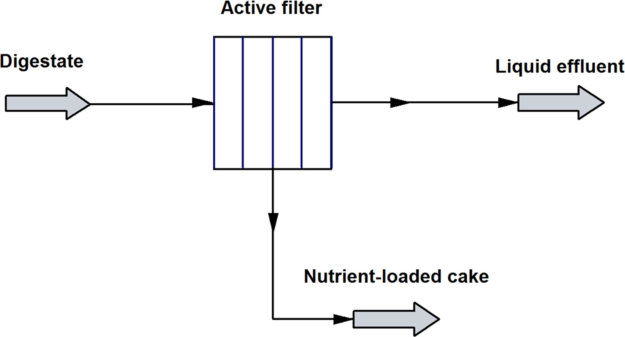
\includegraphics[width=0.6\linewidth, trim={0cm 0cm 0cm 0cm},clip]{gfx/Chapter2/Fig2.pdf} 
	\caption{Scheme of the filter.}
	\label{fig:FilterScheme}
\end{figure}

\begin{equation}
	\begin{aligned}
		& F_i^{{cake}} \ge F_i^{{in}} \cdot \eta _i^{j} - M\cdot \left(1 - {y^j}\right) \\
		& {i} \in \left\{ \text{P, N} \right\} \\
		& j \in \left\{ {{\text{filter media}}} \right\} \label{eq:Eq2}
	\end{aligned}
\end{equation}

\begin{table}[h]
	\centering
	\caption{Recovered P and N yield for different filter media..}
	\label{table:Table3}
%	\resizebox{\columnwidth}{!}{
	\begin{threeparttable}
		\begin{tabular}{@{}ccc@{}}
			\toprule
			Media/nutrient & P (\% recovered) & N (\% recovered) \\ \midrule
			Polonite       & 96.7\textsuperscript{a}           & 18.0\textsuperscript{c}            \\
			Filtra P       & 98.2\textsuperscript{a}           & 50.0\textsuperscript{e}            \\
			Wollastonite   & 51.1\textsuperscript{a}           & 70.0\textsuperscript{d}            \\
			Dolomite       & 44.0\textsuperscript{b}           & 50.0\textsuperscript{e}            \\
			Metal slag     & 85.6\textsuperscript{a}           & 67.0\textsuperscript{f}            \\ \bottomrule
		\end{tabular}
%	}
	\begin{tablenotes}
		\footnotesize
		\item {a}: \citet{gustafsson2008phosphate}
		\item {b}: \citet{pant2001phosphorus}
		\item {c}: \citet{kietlinska2005evaluation}
		\item {d}: \citet{lind2000nutrient}
		\item {e}: \citet{aziz2004removal}
		\item {f}: \citet{yang2009converter}
	\end{tablenotes}
	\end{threeparttable}
\end{table}

\begin{align}
	\sum {{y}}^{{j}} { = 1} \label{eq:Eq3}
\end{align}

\begin{align}
	F_i^{{liquid \ effluent}} = F_i^{{in}} - F_{{i}}^{{cake}} \label{eq:Eq4}
\end{align}
%
\begin{align}
	F_k^{{cake}} = F_k^{{in}}; \ {k} \in \left\{ \text{TS, C ,K} \right\} \label{eq:Eq5}
\end{align}

\begin{align}
	F_{Wa}^{{cake}} = \left( {F_{TS}^{{cake}} + \sum\limits_i {F_i^{{cake}}} } \right) \cdot \frac{C_{Wa}^{cake}}{1 - C_{Wa}^{{cake}}} \label{eq:Eq6}
\end{align}
%%

\begin{align}
	F_{Wa}^{{{liquid \ effluent}}} = F_{Wa}^{{in}} - F_{Wa}^{{cake}} \label{eq:Eq7}
\end{align}

To select among the five filter media, we use a Big M formulation to select one of them assigning a binary variable $y^{\text{filter media}}$ for each filter media, Eqs. \ref{eq:Eq2} and \ref{eq:Eq3}. This variable takes a value of 1 for the selected filter media and 0 for the rest, so that we are able to evaluate one filter media per time.

It is assumed that the cake obtained contains moisture with a value of 55\% in weight basis $\left(C_{Wa}^{cake}\right)$. The optimal filter media among the evaluated compounds is metal slag \citep{li2015study}.

The cost of each alternative has been estimated according to the number of filters, which depends on the maximum flow they can process. The maximum flow per filter unit, $F_{max}^{{filter}}$, is 1,300 ft\textsuperscript{3}/min \citep{loh2002process}. To design the filter units we have taken the minimum value between the flow provided by mass balances and the maximum flow allowed per filter, Eqs. \ref{eq:Eq8}–\ref{eq:Eq10}.

\begin{align}
	F\left( {\frac{\text{ft}^3}{\text{min}}} \right) = \frac{{{F_{in}}}}{{{\rho _{{digestate}}}}} \label{eq:Eq8}
\end{align}

\begin{align}
	{n}_{{filters}} \ge \frac{F_{total}^{{filter}}}{F_{{max}}^{{filter}}} 	\label{eq:Eq9}
\end{align}

\begin{align}
	F_{design}^{{filter}}\left( {\frac{\text{ft}^3}{\text{min}}} \right) = \min \left( {F_{max}^{{filter}},F_{total}^{{filter}}} \right) \label{eq:Eq10}
\end{align}

In fact, since the maximum flow for a cartridge filter is 1,300 ft\textsuperscript{3}/min, for this facility the number of filters considered in this work will always be one and the design flow is equal to the flow provided by mass balances.

The correlation used to calculate the filter cost, Eq. \ref{eq:Eq11}, is obtained from data reported in \citet{loh2002process}. This correlation provides the price in 1998 dollars, so we use the Chemical Engineering Index to update it.

\begin{align}
	FC_{filtration}\left( \text{USD}  \right) = 4.7436\cdot F_{design}^{{filter}} + 807.6923 \label{eq:Eq11}
\end{align}

The operating cost is estimated using a simple correlation, Eq. \ref{eq:Eq14}, where we assume that the utilities contribute 20\% of the total \citep{vian1975pronostico}. The other economical contributions considered are chemicals, estimated as in Eq. \ref{eq:Eq12}, labour, as per Eq. \ref{eq:Eq13}, and the contribution of the investment cost of the units given by Eqs. \ref{eq:Eq10} and \ref{eq:Eq11}. The filter media are considered as chemicals that will be replaces annually.

\begin{align}
	{ChemC}_{filtration}\left(\frac{\text{EUR}}{\text{year}}\right) = 	\frac{F_{P}^{in} \cdot 3600 \cdot h \cdot d}{\frac{kg_P}{kg_{{filter \ media}}}} \cdot {Price}_{{filter \ media}} \label{eq:Eq12}
\end{align}

In Eq. \ref{eq:Eq12}, $kg_{{filter \ media}}$ are calculated as the P content in the inlet stream divided by the filter media P adsorption capacity.

\begin{align}
	& {{Labour \ cost}}\left( \frac{\text{EUR}}{\text{year}} \right) = \label{eq:Eq13} \\
	& \left( 61.33\cdot F_P^{recovered} \cdot 3.6\cdot{{{h}^{\left( { - 0.82} \right)}}} \right) \cdot \left( {F_P^{recovered} \cdot 3.6 \cdot h \cdot d} \right) \cdot \left( {\frac{{Salary}}{{h \cdot d}}} \right)\cdot{n_{OP}} \nonumber 
\end{align}

The number of operations considered, $n_{OP}$ , is equal to 1.

\begin{align}
	&{{Operating \ cost}}\left( \frac{\text{EUR}}{\text{year}} \right) = \label{eq:Eq14}\\ 
	&\frac{{{{ChemC}} + 1.5\cdot{{Labour \ cost}} + 0.3 \cdot Fixed \ Cost\cdot{f_i}\cdot{f_j}}}{{(1 - Utilities)}} \nonumber 
\end{align}

Finally the credit obtained from the cake is computed as the weighted sum of each nutrient value, Eq. \ref{eq:Eq15}, \citep{hernandez2017bio}, and the benefits (or losses) are computed as the difference between the credit obtained from the cake and the operating costs of the facility, Eq. \ref{eq:Eq16}.

\begin{align}
	& Cost_{cake} \left( \frac{\text{EUR}}{\text{year}} \right) = \label{eq:Eq15} \\ 
	& \left( {F_P^{recovered}\cdot{Price_P} + F_N^{recovered}\cdot{Price}_N} + F_K^{recovered}\cdot{Price_K} \right) \nonumber \\
	& \cdot 3600\cdot h \cdot d \nonumber
\end{align}

\begin{align}
	{{Benefits}}_{Filtration} \left(\frac{\text{EUR}}{\text{year}}  \right) = Cost_{cake} - {{Operating \  cost}} \label{eq:Eq16}
\end{align}

\subsubsection{Coagulation}
\begin{figure}[h!]
	\centering
	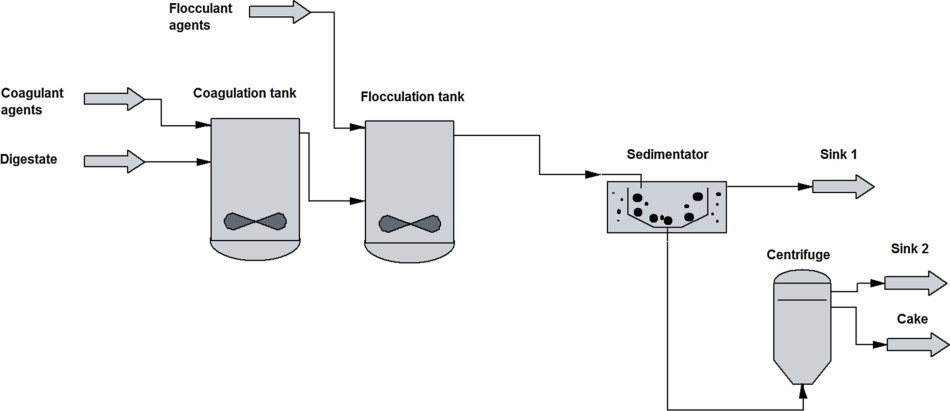
\includegraphics[width=1\linewidth, trim={0cm 0cm 0cm 0cm},clip]{gfx/Chapter2/Fig3.pdf} 
	\caption{Scheme of the coagulation process.}
	\label{fig:CoagScheme}
\end{figure}

Coagulation is a chemical treatment to process the digestate. The goal of this process is to destabilize colloidal suspensions by reducing the attractive forces, followed by a flocculation process to form flocs from the previously destabilized colloids and to subsequently precipitate them. The nutrients are then recovered with other sedimented solids by clarification. Both N and P can be removed from the influent through coagulation–flocculation, where phosphorus is removed primarily in the form of metal hydroxides, which is the dominant process at typical plant pH values \citep{szabo2008significance}. Nitrogen elimination is related to the removal of the colloidal matter \citep{aguilar2002nutrient}. Different coagulation agents are considered aiming at selecting the optimal one: FeCl\textsubscript{3}, Fe\textsubscript{2}(SO\textsubscript{4})\textsubscript{3}, Al\textsubscript{2}(SO\textsubscript{4})\textsubscript{3}, and AlCl\textsubscript{3}. The flowsheet for the process of coagulation is presented in Fig. \ref{fig:CoagScheme}.

The removal efficiency achieved is similar for the different coagulant agents, with values up to 99\% for phosphorus and 57\% for nitrogen \citep{aguilar2002nutrient}. The main variables which influence the coagulation–flocculation process are the initial ratio of metal to phosphorus, pH, and chemical oxygen demand (COD). The initial metal-phosphorus molar ratio must be between 1.5 and 2.0, and the recommended pH range is from 5.5 to 7. COD has a negative impact on the removal efficiency when its value is increased \citep{szabo2008significance}.

To determine the amount of coagulant agent to be added to the system, it has been considered that a metal/phosphorus molar ratio of 1.75 must be achieved \citep{szabo2008significance}. Given the relationship between the P in the raw material stream, the metal added, and the metal concentration in the commercial presentation of the coagulant agent, we are able to compute the coagulant agent amount that should be added. In the coagulation and flocculation tanks the flocs are formed and nutrients are recovered in the sediment together with coagulation agents and organic solids contained in the raw material. In the decanter, it has been considered that the stream with solids has a water content of 50\% $\left(C^{sedimentator}_{Wa}\right)$ \citep{williams2011digestates} and the water content of the centrifuge outlet solids stream is 60\% $\left(C^{centrifuge}_{Wa}\right)$ \citep{wakeman2007separation}.

Other elements present in the digestate, such as total solids, carbon, and potassium are assumed to be present in the solid forming compounds that sediment. Thus, they are among species that constitute the cake. Taking into account the elements mentioned above mass balances have been formulated with the corresponding removal ratios. To select and evaluate the different coagulant agents, the problem has been modelled using a mixed-integer nonlinear programming (MINLP) formulation with Big-M constraints, Eqs. \ref{eq:Eq17} and \ref{eq:Eq18}.

\begin{align}
	& F_j^{{{coag \ tank}}} \ge \frac{F_P^{in}}{MW_P} \cdot MeP_{ratio} \cdot \frac{MW_j}{C_{Me}} - M \cdot \left(1 - {y^j}\right) \label{eq:Eq17} \\
	& {j} \in \left\{ \text{coagulant agents} \right\} \nonumber
\end{align}

\begin{align}
	\sum {{{{y}}^j}} = 1 \label{eq:Eq18}
\end{align}

where $MeP$ is the metal/phosphorus ratio and M is a large value to formulate the Big-M constraint to select and evaluate the different coagulant agents. Mass balances are computed using Eqs. \ref{eq:Eq19}–\ref{eq:Eq28}.

\begin{align}
	& F_j^{{{coag \ tank}}} = F_j^{{{floc \ tank}}} = F_j^{{{sedimentator}}} = F_j^{{{centrifuge}}} = F_j^{{{cake}}} \label{eq:Eq19}\\
	& j \in \left\{ \text{coagulants} \right\} \nonumber
\end{align}

\begin{align}
	& F_i^{in} = F_i^{{{coag \ tank}}} = F_i^{{{floc \ tank}}} = F_i^{{{sedimentator}}} \label{eq:Eq20} \\
	& {i} \in \left\{ \text{P, N} \right\} \nonumber
\end{align}

\begin{align}
	F_i^{cake} = F_i^{centrifuge} = F_i^{{{sedimentator}}} \cdot \eta_i^j \label{eq:Eq21}
\end{align}

\begin{align}
	F_i^{{{sink1}}} = F_i^{{{sedimentator}}} - F_i^{{{centrifuge}}} \label{eq:Eq22}
\end{align}

\begin{align}
	& F_k^{in} = F_k^{{{coag \ tank}}} = F_k^{{{floc \ tank}}} = F_k^{{{sedimentator}}} = F_k^{{{centrifuge}}} = {{F}}_{{k}}^{{{cake}}} \label{eq:Eq23} \\
	& {{k}} \in \left\{ \text{TS, C, K} \right\} \nonumber
\end{align}

\begin{align}
	F_{Wa}^{in} = F_{Wa}^{{{coag \ tank}}} = F_{Wa}^{{{floc \ tank}}} = F_{Wa}^{{{sedimentator}}} \label{eq:Eq24}
\end{align}

\begin{align}
	& {F}_{{Wa}}^{centrifuge} = \label{eq:Eq25} \\
	& \left( {{F}_{TS}^{centrifuge} + \sum\limits_i {{F}_i^{centrifuge} + \sum\limits_j {F}_j^{centrifuge}} }  \right) \cdot \frac{{C_{Wa}^{sedimentator}}}{1 - C_{Wa}^{centrifuge}} \nonumber
\end{align}

\begin{align}
	{F}_{Wa}^{sink1} = F_{Wa}^{sedimentator} - {F}_{Wa}^{centrifuge} \label{eq:Eq26}
\end{align}

\begin{align}
	{F}_{Wa}^{cake} = \left( {F}_{TS}^{cake} + \sum\limits_i {F_i^{cake} + \sum\limits_j {F}_j^{cake}}  \right) \cdot \frac{{C_{Wa}^{centrifuge}}}{{1 - C_{Wa}^{centrifuge}}} \label{eq:Eq27}
\end{align}

\begin{align}
	{F}_{Wa}^{sink2} = F_{Wa}^{centrifuge} - F_{Wa}^{cake} \label{eq:Eq28}
\end{align}

The estimation of the size and cost of both the coagulation and flocculation tanks has been carried out using a correlation developed by \citet{almena2016technoeconomic} as a function of the weight of the vessels. To simplify the mass balances it is considered that the volume provided by the coagulant agents is negligible with respect to the processed stream of the digestate. The vessel size is computed from the residence time. The hydraulic retention time considered in the coagulation tank is 4 min \citep{zhou2008enhanced}. The vessel size is computed from the residence time, Eq. \ref{eq:Eq29}. Using these data, the diameter and length are computed using rules of thumb, Eqs. \ref{eq:Eq30} and \ref{eq:Eq31}. Finally, a correlation for the thickness as a function of the diameters allows determining the mass of metal required for the vessel and its weight, Eqs. \ref{eq:Eq32} and \ref{eq:Eq33}. Vessel cost estimation is provided by Eq. \ref{eq:Eq34}.

\begin{align}
	{V}_{Coag tank}\left( \text{m}^{3} \right) = HR{T_{Coag \ tank}} \cdot \frac{F_{digestate}^{in}}{\rho_{digestate}} \label{eq:Eq29}
\end{align}

\begin{align}
	{D_{Coag \ tank}} \left( \text{m} \right) = \left( \frac{6 \cdot{V}_{Coag \ tank}}{7 \cdot \pi} \right)^{1/3} \label{eq:Eq30}
\end{align}

\begin{align}
	{L_{{{Coag \ tank}}}}\left( m \right) = 4\cdot{D_{Coag \ tank}} \label{eq:Eq31}
\end{align}

\begin{align}
	{e_{Coag \ tank}}\left( \text{m} \right) = 0.0023 + 0.003\cdot{D_{{{Coag \ tank}}}} \label{eq:Eq32}
\end{align}

\begin{align}
	& {W_{Coag \ tank}}\left( \text{kg} \right) = {\rho_{SS316}}\cdot \label{eq:Eq33} \\
	& \Bigg[ \pi \cdot \left( {{{\left( \frac{{{D_{Coag tank}}}}{2} + {e_{Coag \ tank}} \right)}^2} - {{\left( \frac{{{D_{Prec \ tank}}}}{2} \right)}^2}} \right)\cdot{L_{Coag \ tank}} + \nonumber \\ 
	& \frac{4}{3} \cdot \pi \cdot \left( \left( \frac{D_{Coag \ tank}}{2} + {e_{Coag \ tank}} \right)^3 - \left( \frac{D_{Coag \ tank}}{2} \right)^3 \right) \Bigg] \nonumber
\end{align}

\begin{align}
	{Cost}_{Vessel} \left( \text{USD} \right) = 6839.8 \cdot {V}_{Coag \ tank}{\left( {\text{m}^{3}} \right)^{0.65}} \label{eq:Eq34}
\end{align}

To estimate the power consumed by the agitator, Eq. \ref{eq:Eq35}, rules of thumb have been used; where the specific power consumed, $\kappa_{agitator}$, is tabulated in \citet{walas1988chemical}. For our slurries a value of $\kappa_{agitator}$ equal to 10 HP per 1000 US gallons is the most appropriate.

\begin{align}
	P_{Agitator}\left( \text{HP} \right) = V_{Coag \ tank} \left( {\text{US gallon}} \right) \cdot \frac{\kappa_{agitator}}{1000} \label{eq:Eq35}
\end{align}

The agitator cost is also estimated using a correlation from \citet{walas1988chemical}, Eq. (36). For cost estimation purposes we have considered stainless steel 316 as construction material and a dual impeller operating at speed between 56 and 100 rpm depending on the tanks size. With these considerations the values for $a$, $b$ and $c$ are 8.8200, 0.1235 and 0.0818 respectively \citep{walas1988chemical}. This correlation provides the cost in 1985 dollars, so it is necessary to update the result using the Chemical Engineering Index as before.

\begin{align}
	Cost_{Agitator} \left( \text{USD}_{1985}  \right) = {e^{a + b \cdot {\text{ln}}\left( {{P_{agitator}}\left( \text{HP} \right)} \right) + c \cdot {\left[ \text{ln}\left( {P_{agitator}\left( \text{HP} \right)} \right) \right] }^2}} \label{eq:Eq36}
\end{align}

The total cost of the coagulation tank is equal to the sum of the vessel cost and the agitator cost, Eq. \ref{eq:Eq37}.

\begin{align}
	{Cost}_{Coag \ tank} = Cost_{Vessel} + Cost_{Agitator} \label{eq:Eq37}
\end{align}

The flocculation tank is designed similarly to that of the coagulation, using Eqs. \ref{eq:Eq29}–\ref{eq:Eq37}. For this step the hydraulic retention time is 25 min \citep{zhou2008enhanced}.

The decanter is assumed to be circular because of its lower operating and maintenance costs. The area, Eq. \ref{eq:Eq38}, is computed using the parameter $A_{specific}$, which is the specific clarifier area in m\textsuperscript{2} per ton of inlet flow per day \citep{wef2005wef}. The typical value, 10 m\textsuperscript{2}/(t/day), is taken from \citet{green2008perry}. The diameter of the clarifier, Dclarifier , is computed from the area value, Eq. \ref{eq:Eq39}.

\begin{align}
	{A}_{clarifier} \left( \text{m}^2 \right) = \frac{A_{specific} \cdot F_{digestate}^{in}\left( \frac{\text{m}^3}{\text{day}} \right)}{1000} \label{eq:Eq38}
\end{align}

\begin{align}
	D_{clarifier} \left( \text{m} \right) = \left( \frac{4 \cdot A_{clarifier}}{\pi} \right)^{1/2} \label{eq:Eq39}
\end{align}

The number of clarifiers is an integer value that is computed as the minimum integer from the ratio between the clarifier diameter calculated before and the maximum clarifier diameter, $D_{max}^{clarifier}$, Eq. \ref{eq:Eq40}. The maximum clarifier diameter value considered is 40 m \citep{green2008perry}.

\begin{align}
	{n}_{clarifiers} \ge \frac{D^{clarifier}}{D_{max}^{clarifier}} \label{eq:Eq40}
\end{align}

The diameter used in the final design will be the smallest between $D^{clarifier}$ and $D_{max}^{clarifier}$, Eq. \ref{eq:Eq41}.

\begin{align}
	D_{design}^{clarifier} \left( \text{m} \right) = \text{min}(D_{max}^{clarifier},D^{clarifier}) \label{eq:Eq41}
\end{align}

To model the minimization function and compute $D_{design}^{clarifier}$, the following smooth function approximation, given by Eq. \ref{eq:Eq42}, is used based on previous work \citep{de2016characterization} to avoid discontinuities within the problem formulation.

\begin{align}
	D_{design}^{clarifier} \left( \text{m} \right) = \frac{D_{max}^{clarifier}}{1 + {e^{\left( -F_{digestate}^{in} + 0.342 \right) \cdot 2.718}}} \label{eq:Eq42}
\end{align}

The cost estimation correlation has been developed from the data in \citet{wef2005wef}, Eq. \ref{eq:Eq43}. It includes all the items involved in the operation of such an unit. The correlation must be updated to current prices using the Chemical Engineering Index.

\begin{align}
	Cost_{clarifier} \left( \text{USD}_{1979} \right) = \left( 13060 \cdot D_{design}^{clarifier} - 58763 \right) \cdot {n}_{clarifiers} \label{eq:Eq43}
\end{align}

Centrifuge sizing and costing is based on the data by \citet{green2008perry}. We assume pusher type with a maximum diameter of 1250 mm. The modelling equation for sizing is given in Eq. \ref{eq:Eq44}.

\begin{align}
	D_{Centrifuge}\left( \text{in} \right) = 0.3308 \cdot \frac{F_{digestate}^{in}}{1000}\cdot 3600 + 9.5092 \label{eq:Eq44}
\end{align}

The number of centrifuges is calculated taking into account the maximum centrifuge diameter, Eq. \ref{eq:Eq45}, and the diameter used in the final design will be the minimum value between D Centrifuge and D Centrifuge max , Eq. \ref{eq:Eq46}.

\begin{align}
	{n}_{centrifuges} \ge \frac{D^{centrifuge}}{D_{max}^{centrifuge}} \label{eq:Eq45}
\end{align}

\begin{align}
	D_{design}^{centrifuge} = \min \left( {D_{max}^{centrifuge}, D^{centrifuge}} \right) \label{eq:Eq46}
\end{align}

As in the clarifier, we develop a smooth approximation, Eq. \ref{eq:Eq47}, to compute the design diameter avoiding discontinuities as follows:

\begin{align}
	D_{design}^{centrifuge} = \frac{D_{max}^{centrifuge}}{1 + {e^{\left( { -F_{digestate}^{in} + 35.369} \right) \cdot 0.0395}}} \label{eq:Eq47}
\end{align}

The cost for the centrifuge is estimated based on the data by \citet{green2008perry} as a function of its diameter, Eq. \ref{eq:Eq48}. Since the cost correlation is based on 2004 values, the Chemical Engineering Index it used to update the equipment cost.

\begin{align}
	& Cost_{centrifuge}\left( \text{USD}_{2004}  \right) = \label{eq:Eq48} \\
	& \left( {10272 \cdot D_{design}^{centrifuge} - 24512} \right) \cdot {n}_{centrifuges} \nonumber
\end{align}

We estimate the operating cost of this system by accounting for the annualized equipment cost (fixed cost), chemicals and labor cost. A similar procedure as before is followed \citep{vian1975pronostico} but for the clarifier fixed costs as the correlation to estimate its costs already includes the operating cost, Eq. \ref{eq:Eq49}.

\begin{align}
	& FC_{coagulation} \left( \frac{ \text{EUR} }{\text{year}} \right) = \label{eq:Eq49}\\
	& \left( {Cost}_{Coag \ tank} + {Cost}_{Floc \ tank} + Cost_{centrifuge} \right) \cdot {f_i} \cdot {f_j} + Cost_{clarifier} \nonumber
\end{align}

The chemicals costs are estimated as Eq. \ref{eq:Eq50}.

\begin{align}
	& {ChemC}_{coagulation} \left( \frac{ \text{EUR} }{\text{year}} \right) = \label{eq:Eq50} \\
	& \big( F_{Fe_2 \left(SO_{4} \right)_3}^{in} \cdot Price_{Fe_2 \left( SO_{4} \right)_3} + F_{Al_{2} \left( SO_{4} \right)_3}^{in} \cdot Price_{Al_{2} \left( SO_{4} \right)_3} + \nonumber \\
	& F_{FeCl_{3}}^{in} \cdot Price_{FeCl_{3}} + F_{AlCl_{3}}^{in} \cdot Price_{AlCl_{3}} \big) \cdot 3600\cdot h \cdot d \nonumber
\end{align}

To estimate the price for the cake, as in the previous case, we assume the price of each of the nutrients contained (N, P, and K). The price for each nutrient is taken same as before. Thus, the cake price is computed as the weighted sum of each nutrient, as in Eq. \ref{eq:Eq15} \citep{hernandez2017bio}.

Finally, the economic benefits or losses of operating this system are calculated as the difference between the credit obtained from the cake and the operating costs of section of the facility, as in Eq. \ref{eq:Eq16}.

\subsubsection{Centrifugation}
Centrifugation is a pretreatment that separates solid and liquid phases and that can be used to recover nutrients from the digestate. The advantage of this system is the simple equipment used. Precipitant agents can be added to improve the removal efficiency significantly. Previous studies show that an appropriate mixture of CaCO\textsubscript{3} and FeCl\textsubscript{3} promotes nutrients recovery. In particular, a ratio of 0.61 kg CaCO\textsubscript{3} per kilogram of total solids in the raw material inlet stream, and 0.44 kg of FeCl\textsubscript{3} per kilogram of total solids in the raw material inlet stream, achieves a removal efficiency up to 95\% and 47\% for P and N respectively \citep{meixner2015effect}. Fig. \ref{fig:CentrifScheme} presents a scheme of the process.

\begin{figure}[h!]
	\centering
	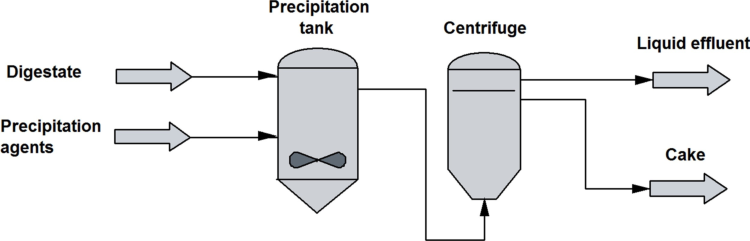
\includegraphics[width=0.8\linewidth, trim={0cm 0cm 0cm 0cm},clip]{gfx/Chapter2/Fig4.pdf} 
	\caption{Scheme for the centrifugation treatment.}
	\label{fig:CentrifScheme}
\end{figure}

Centrifugation process consists of two units, a precipitation tank where CaCO3 and FeCl3 are added, and the centrifuge. These equipment have been modeled using mass balances and removal ratios for the precipitating species. Note that the total solids, carbon, and potassium are assumed to be present in the form of solid compounds, so they will be removed as part of the cake. Moreover, the water content of the centrifuge outlet solids stream is assumed to be 60\% $\left(C_{Wa}^{centrifuge}\right)$ \citep{wakeman2007separation}. Mass balances for the process have been evaluated in Eqs. \ref{eq:Eq51}-\ref{eq:Eq59}:

\begin{align}
	& F_j^{in} = F_{TS}^{in} \cdot \frac{\varphi _{j}}{C_{j}} \label{eq:Eq51} \\
	& {j} \in \left\{ {\text{precipitation agents}} \right\} \nonumber
\end{align}

\begin{align}
	F_j^{in} = F_j^{prec \ tank} = F_j^{centrifuge} = F_j^{cake} \label{eq:Eq52}
\end{align}

\begin{align}
	& F_i^{in} = F_i^{prec \ tank} = F_i^{centrifuge} \label{eq:Eq53} \\
	& {i} \in \left\{ {{\text{P, N}}} \right\} \nonumber
\end{align}

\begin{align}
	F_i^{cake} = F_i^{centrifuge} \cdot {\eta_i} \label{eq:Eq54}
\end{align}

\begin{align}
	F_i^{liquid \ effluent} = F_i^{centrifuge} - F_i^{cake} \label{eq:Eq55}
\end{align}

\begin{align}
	& F_k^{in} = F_k^{prec \ tank} = F_k^{centrifuge} = F_k^{cake} \label{eq:Eq56} \\
	& {k} \in \left\{ \text{TS, C, K} \right\} \nonumber
\end{align}

\begin{align}
	F_{Wa}^{in} = F_{Wa}^{prec \ tank} = F_{Wa}^{centrifuge} \label{eq:Eq57}
\end{align}

\begin{align}
	{F}_{Wa}^{cake} = \left( {F}_{TS}^{cake} + \sum\limits_i {F}_i^{cake} + \sum\limits_j {F}_j^{cake} \right) \cdot \frac{C_{Wa}^{centrifuge}}{1 - C_{Wa}^{centrifuge}} \label{eq:Eq58}
\end{align}

\begin{align}
	{F}_{Wa}^{liquid \ effluent} = F_{Wa}^{centrifuge} - {F}_{Wa}^{cake} \label{eq:Eq59}
\end{align}

where $\varphi _{j}$ is the precipitation agent per total solids mass ratio (0.61 kg CaCO\textsubscript{3}/kg TS and 0.44 kg FeCl\textsubscript{3} /kg TS).

These units have been designed using correlations as a function of the flow processed. For the design of the precipitation tank (volume, diameter, length, thickness, weight, and cost calculations) the equations provided by \citet{almena2016technoeconomic} have been used as before, Eqs. \ref{eq:Eq29}-\ref{eq:Eq37}, considering a hydraulic retention time of 2.5 min \citep{szabo2008significance}.

\begin{align}
	{V}_{Prec tank} \left( \text{m}^{3} \right) = HRT_{Prec \ tank} \cdot \left( \frac{F_{digestate}^{in}}{\rho_{digestate}} + \frac{F_{FeCl_{3}}^{in}}{\rho _{FeCl_{3}}} \right) \label{eq:Eq60}
\end{align}

The volume of CaCO\textsubscript{3} added is assumed negligible compared to the volume of the liquid because it is added as a solid. Thus, the diameter of the tanks is computed using Eqs. \ref{eq:Eq60} and \ref{eq:Eq30} as in the previous unit. The cost of the vessel is given by the weight of the metal, using the correlations provided by \citep{almena2016technoeconomic}, Eqs. \ref{eq:Eq31}-\ref{eq:Eq34}. The power required is computed, as in previous cases, using the rules of thumb in \citep{walas1988chemical}, Eq. \ref{eq:Eq35}, where the value of $\kappa_{agitator}$ agitator is equal to 10 HP per 1000 gal, in accordance with the data collected in the literature \citet{walas1988chemical}. The cost correlation is given by Eq. \ref{eq:Eq36} and updated to 2016 prices. The total cost of the precipitation tank included the vessel and the agitator costs, Eq. \ref{eq:Eq37}.

The centrifuge size is characterized by its diameter. We model it as in the previous technologies using Eqs. \ref{eq:Eq44}-\ref{eq:Eq48}. The operating costs involve fixed, chemicals and labour costs. Fixed costs are estimated using Eq. \ref{eq:Eq61}. The labor cost is estimated in Eq. \ref{eq:Eq13}, where $n_{OP}$ is equal to 1 \citep{vian1975pronostico}. Total operating cost is given by Eq. \ref{eq:Eq14}. The chemicals costs involve the consumption of CaCO\textsubscript{3} and FeCl\textsubscript{3}, and it is estimated using Eq. \ref{eq:Eq62}:

\begin{align}
	{FC}_{centrifugation} \left( \frac{\text{EUR}}{\text{year}} \right) = \left( {Cost_{centrifuge}} + {Cost}_{Prec \ tank} \right) \cdot {f_i} \cdot {f_j} \label{eq:Eq61}
\end{align}

\begin{align}
	& {ChemC}_{centrifugation} \left( \frac{\text{EUR}}{\text{year}} \right) = \label{eq:Eq62} \\
	& \left( F_{CaCO_{3}}^{in} \cdot {Price}_{CaCO_{3}} + F_{FeCl_{3}}^{in} \cdot {Price}_{FeCl_{3}} \right) \cdot 3600 \cdot h \cdot d \nonumber
\end{align}

The cake recovered is the main asset of the process. Its price is estimated as the weighted sum of each nutrient, Eq. \ref{eq:Eq15}, \citep{hernandez2017bio}. Finally, the benefits or losses of operating this system are calculated as the difference between the revenue obtained from the cake and the operating costs of the facility, Eq. \ref{eq:Eq16}.

\subsubsection{Struvite production}
P and N can be recovered from digestate through the formation of struvite, which is a phosphate mineral with a chemical formula of MgNH\textsubscript{4}PO\textsubscript{4} ·6H\textsubscript{2}O. The advantage of this technology is that struvite is a solid with a high nutrients density, it is easy to transport, and it can be used as slow-release fertilizer without any post-processing \citep{doyle2002struvite}. The removal of nutrients via struvite production follows the reaction below, requiring the addition of MgCl\textsubscript{2}, resulting in the production of struvite crystals that can be recovered as solid:

\begin{align}
	\text{Mg}^{2+} + \text{NH}_4^{+}  + \text{H}_{\text{n}}\text{PO}_4^{3-n} + 6\text{H}_{2}\text{O} \leftrightarrow \text{MgNH}_{4}\text{PO}_{4} \cdot 6\text{H}_{2}\text{O} + \text{nH}^{+} \label{eq:Eq63}
\end{align}

Due to the presence of potassium in the digestate, together with struvite, another product called potassium struvite or K-Struvite, is also produced. In this case the ammonia cation is substituted by the potassium cation \citep{wilsenach2007phosphate}.

\begin{align}
	\text{K}^{+} + \text{Mg}^{2+} + \text{H}_{\text{n}}\text{PO}_4^{3-n} + 6\text{H}_{2}\text{O} \leftrightarrow \text{KMgPO}_{4}\cdot 6\text{H}_{2}\text{O} + \text{nH}^{+} \label{eq:Eq64}
\end{align}

Since the formation of struvite is favored over the formation of K-Struvite, it is considered that only 15\% of the potassium contained in the digestate will react to form K-Struvite \citep{zeng2006nutrient}. The mass balance for the reactors is given by the stoichiometry of the reactions above.

Two different types of reactors can be used to obtain struvite, either a stirred tank (CSTR) or a fluidized bed reactor (FBR). Figs. \ref{fig:FBRScheme} and \ref{fig:CSTRScheme} provide detailed flowsheets of each case. In case of the FBR, struvite is recovered from the bottoms and the liquid must be processed in a hydrocyclone to avoid discharging fines. In the case of CSTR tanks, we need to use a centrifuge to recover the struvite. We can help the crystal growth by seeding \citep{doyle2002struvite, kumashiro2001pilot}. Due to the substantial increase in the struvite formation yield, we consider the addition of struvite seeds in both cases. The reaction takes place at about 27 \textdegree C, with the addition of MgCl\textsubscript{2} at a concentration of 57.5 mg/dm\textsuperscript{3} \citep{zhang2014phosphate}. A Mg:P molar ratio of 2 \citep{bhuiyan2008phosphorus} is used.

\begin{figure}[h!]
	\centering
	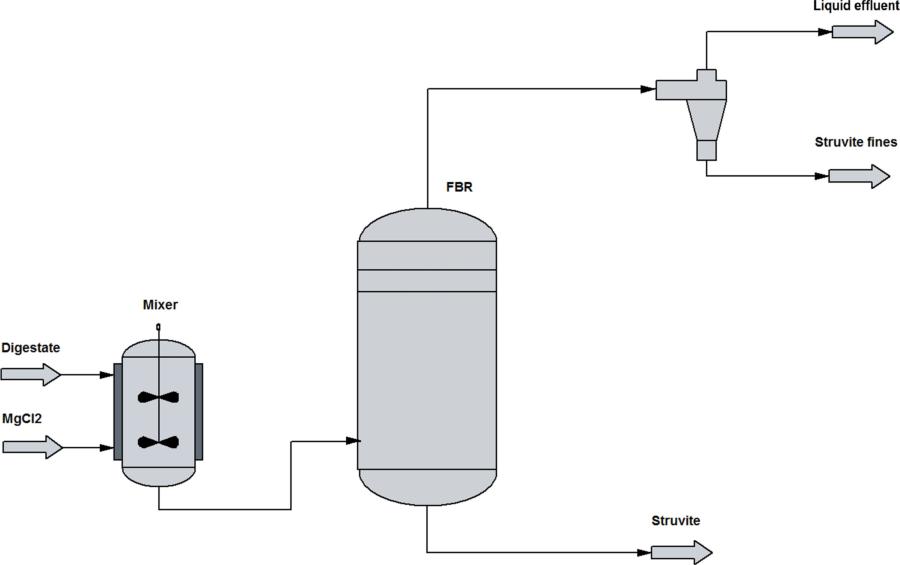
\includegraphics[width=0.8\linewidth, trim={0cm 0cm 0cm 0cm},clip]{gfx/Chapter2/Fig5.pdf} 
	\caption{Scheme for the FBR system.}
	\label{fig:FBRScheme}
\end{figure}

\begin{figure}[h!]
	\centering
	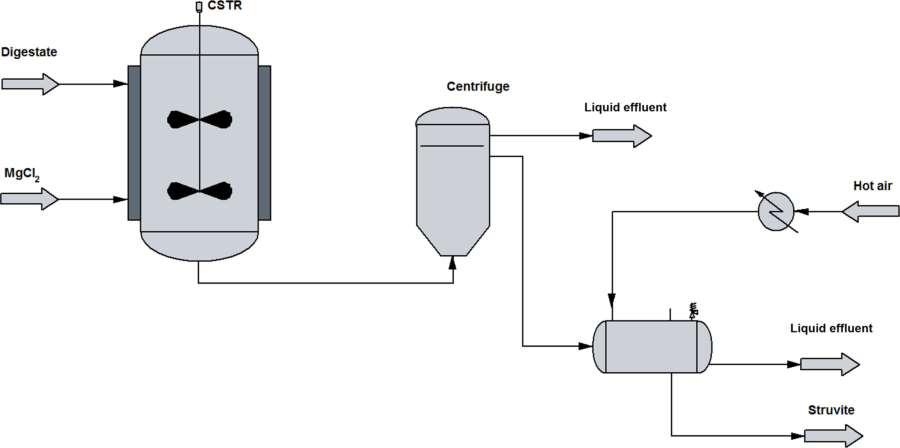
\includegraphics[width=0.8\linewidth, trim={0cm 0cm 0cm 0cm},clip]{gfx/Chapter2/Fig6.pdf} 
	\caption{Scheme for the CSTR based struvite production system.}
	\label{fig:CSTRScheme}
\end{figure}

The FBR system is composed of three elements: a mixer tank, a FBR rector, and a hydrocyclone. The system operation consists of a digestate flow which is mixed with a stream of MgCl\textsubscript{2} in the mixing tank. The addition of MgCl\textsubscript{2} helps precipitate the struvite by increasing the concentration of the species inside the reactor. As the concentration of NH\textsuperscript{4+} is high due to the pH, and the inorganic N and P are the elements we want to recover, the only element which is necessary to be added is Mg in form of MgCl\textsubscript{2}.

In the tank there is a suspension of struvite seeds with a size of 0.8 mm which promote the precipitation of struvite. The solid struvite is evacuated from the reactor at the bottom and its moisture is low enough to avoid the use of a dryer. The other stream which leaves the reactor contains liquid water in a high proportion with the excess of Mg, the total solids from the digestate, and low amounts of nutrients and other components. This stream is introduced in a hydrocyclone to recover fines of struvite which can be removed by this stream. 100\% of fines removal is assumed but no fines production is considered in the model.

To estimate the cost of this system we evaluate the effect of the following variables, whose operating values are shown between parenthesis:

\begin{itemize}
	\item Digestate input mass and volume flow (between 1 and 100 kg/s)
	\item Recovered struvite humidity (5\% in mass)
	\item Amount of phosphorus recovered (90\%)
	\item Mg:P molar ratio with a value of 2
\end{itemize}

In an FBR there are some variables which influence in the design and hence the cost. The variables considered in this work are showed below with the typical values used in the present study between parenthesis:

\begin{itemize}
	\item $d_p$: bed particle diameter, assumed to be 0.8 mm \citep{jordaan2011development}
	\item Sphericity: 0.6 is a standard sphericity for particles used in fluidized bed reactors \citep{Fogler2005Elements}
\end{itemize}

Furthermore, the reaction kinetics and equilibrium are considered to estimate the residence time in the reactor. A first order kinetics, developed by \citep{nelson2003struvite}, has been used, Eqs. \ref{eq:Eq65} and \ref{eq:Eq66}. The kinetic constant is $3.42 \cdot 10^{-3}$ s \textsuperscript{-1} for a pH of 9.

\begin{align}
	\frac{{-dC}}{{dt}} = k \left({C - {C_{eq}}} \right) \label{eq:Eq65}
\end{align}

\begin{align}
	\ln \left( {C - {C_{eq}}} \right) =  - kt + \ln \left( {{C_0} - {C_{eq}}} \right) \label{eq:Eq66}
\end{align}

Struvite formation is an equilibrium reaction. We use the equilibrium ion activity product $\left(IAP_{eq}\right)$ value of $7.08 \cdot 10^{-14}$ \citep{nelson2003struvite} to calculate the equilibrium concentrations in the kinetic model, Eq. \ref{eq:Eq67}. We assumed that the values of ions concentration are equal to ions activity.

\begin{align}
	IAP_{eq} = \left( {Mg^{2+}} \right)\left( NH_4^{+} \right)\left( {PO_4^{3-}} \right) = 7.08 \cdot {10^{ - 14}}  \label{eq:Eq67}
\end{align}

Minimum fluidization velocity is calculated in the first step by considering that the fluid stream is a liquid \citep{mangin2004fluid}. This consideration is motivated because the liquid digestate works as fluidization agent \citep{le2006understanding}. The digestate density is 950 kg/m\textsuperscript{3} \citep{rigby2011new}. The expression used to calculate $u_{mf}$ through Reynolds and Archimedes numbers is given by Eq. \ref{eq:Eq68}, \citep{tisa2014basic}.

\begin{align}
	{u_{mf}} = \frac{Re_{l \ mf} \cdot {\mu_{digestate}}}{\rho_{digestate} - {d_p}} \label{eq:Eq68}
\end{align}

Eq. \ref{eq:Eq68} parameters are determined by Eqs. \ref{eq:Eq69} and \ref{eq:Eq70}.

\begin{align}
	Re_{l \ mf} = \sqrt {33.72 + 0.0404Ar_{l}{\left( {1 - {\alpha_{mf}}} \right)^3}} - 33.7 \label{eq:Eq69}
\end{align}

\begin{align}
	Ar_{l} = \rho_{digestate} \left( {\rho_{struvite} - {\rho _{digestate}}} \right) g \frac{d_p^3}{\mu_{digestate}^2} \label{eq:Eq70}
\end{align}

If the flow has no gas phase, $\alpha_{mf}$ is equal to zero. The terminal velocity is computed using Eq. \ref{eq:Eq71} \citep{tisa2014basic}.

\begin{align}
	{u_t} = \left( \frac{1.78 \cdot {10}^{ - 2} \cdot {\eta ^2}}{\rho_{digestate} \cdot \mu _{digestate}} \right)^{1/3} {d_p} \label{eq:Eq71}
\end{align}

where the parameter $\eta$ is given by Eq. \ref{eq:Eq72}:

\begin{align}
	\eta  = g\left( {\rho _{struvite} - {\rho _{digestate}}} \right) \label{eq:Eq72}
\end{align}

Finally, the fluid velocity $u_0$ must be between $u_{mf}$ and $u_t$. A superficial velocity equal to five times the minimum fluidization velocity is selected \citep{tejero2004optimization}, Eqs. \ref{eq:Eq73} and \ref{eq:Eq74}.

\begin{align}
	{u_{mf}} < {u_0} < {u_t} \label{eq:Eq73}
\end{align}

\begin{align}
	{u_0} = 5 \cdot {u_{mf}} \label{eq:Eq74}
\end{align}

Once the superficial velocity is computed, the area and diameter can be calculated from the mass flow Eqs. \ref{eq:Eq75} and \ref{eq:Eq76}.
\begin{align}
	{A_{FBR}} = \frac{F_{digestate}^{in}}{u_0} \label{eq:Eq75}
\end{align}

\begin{align}
	{D_{FBR}} = \sqrt {\frac{4{A_{FBR}}}{\pi}} \label{eq:Eq76}
\end{align}

The length of the bed is determined by the residence time through the kinetics and the equilibrium ion activity product presented above. Consequently, the magnesium and ammonium concentrations can be calculated from the digestate mass balance and the external magnesium added. Using the $IAP_{eq}$ value, the phosphate concentration in equilibrium at the operational conditions can be determined. This equilibrium value will be used in kinetics, Eq. \ref{eq:Eq77}.

\begin{align}
	t = \frac{\ln \left( {C_0} - {C_{eq}} \right) - \ln \left( C - {C_{eq}} \right)}{k} \label{eq:Eq77}
\end{align}

Thus, the bed length is computed as per Eq. \ref{eq:Eq78}. Typically, the length of the reactor must be 15\% larger than the bed, Eq. \ref{eq:Eq79}.

\begin{align}
	L_{bed} = \frac{u_0}{t} \label{eq:Eq78}
\end{align}

\begin{align}
	L_{FBR} = 1.15 \cdot L_{bed} \label{eq:Eq79}
\end{align}

The estimation of the rector cost is carried out assuming that it is a vessel as presented in the processes above, Eqs. \ref{eq:Eq30}-\ref{eq:Eq34} \citep{almena2016technoeconomic}. The cost of the mixer tank is also estimated as that of a vessel, using Eqs. \ref{eq:Eq29}-\ref{eq:Eq34}, with a volume given by that to provide a hydraulic retention time of 150 s \citep{szabo2008significance}. The impeller is also designed using the same procedure as before, Eqs. \ref{eq:Eq35} and \ref{eq:Eq36} \citep{walas1988chemical}.

Finally, to estimate the cost of the hydrocyclone, a surrogate model using data from Matche website has been developed \citep{Matche} (\url{www.matche.com}). There is a maximum diameter, therefore, if a unit larger than the standard is required, we actually need to duplicate the equipment, Eq. \ref{eq:Eq81}. To estimate the diameter, we considered that there is a linear relationship between the diameter and the flow based on rules of thumb in design literature. A typical unit size of a 20 in diameter hydrocyclone can process 1,000 US gallons per min, Eq. \ref{eq:Eq80} \citep{walas1988chemical}.

\begin{align}
	{D}_{hydrocyclone}\left( {\text{in}} \right) = F_{digestate}^{in} \left( \frac{\text{US gallon}}{\text{min}} \right) \cdot \frac{20}{1000} \label{eq:Eq80}
\end{align}

\begin{align}
	{n}_{hydrocyclone} \ge \frac{D^{hydrocyclone}}{D_{max}^{hydrocyclone}} \label{eq:Eq81}
\end{align}

where ${n}_{hydrocyclone}$ is an integer. The maximum diameter for a hydrocyclone, $D_{max}^{hydrocyclone}$,  is 30 inch based on standard sizes (\url{www.matche.com}).  Thus, the design diameter is the lower diameter between $D^{hydrocyclone}$ and $D_{max}^{hydrocyclone}$, Eq. \ref{eq:Eq82}.

\begin{align}
	D_{design}^{hydrocyclone} = \min (D_{total}^{hydrocyclone}, \ D_{max}^{hydrocyclone}) \label{eq:Eq82}
\end{align}

The estimation of the cost for the fines recovery equipment is computed using Eq. \ref{eq:Eq83} and updated as explained above.

\begin{align}
	& Cost_{hydrocyclone} \left( \text{USD}_{2014} \right) = \label{eq:Eq83} \\
	& {n}_{hydrocyclone} \cdot \left( {2953.2} \cdot D_{design}^{hydrocyclone} - 34,131 \right) \nonumber
\end{align}

The CSTR process consists of four elements: the CSTR reactor, a centrifuge, and a dryer with its corresponding heat exchanger. As the residence time in the CSTR is large enough, it is not necessary to use a mixing tank and MgCl\textsuperscript{2} is added directly in the reactor. Thus, struvite is formed in one step in the CSTR. Since the digestate already contains NH4\textsuperscript{+} and P, we need to add MgCl\textsuperscript{2}. As a result, struvite precipitates, and it is recovered from the bottoms of the reactor and dried in a two step process. The first step consists of a centrifuge that recovers struvite with 5\% (on weight basis) water \citep{baasal1989preliminary}. Next, a drum dryer is implemented to remove the residual moisture to reach commercial standards and reduce transportation costs. Fig. \ref{fig:CSTRScheme} shows the details of the flowsheet. 

The design of the units involved in this process and their cost estimation is based on the following variables:

\begin{itemize}
	\item Digestate input mass and volume flow (between 1 and 100 kg/s)
	\item Recovered struvite humidity (5\% in mass)
	\item Amount of phosphorus recovered (90\%)
	\item Mg:P molar ratio with a value of 2
\end{itemize}

The CSTR is assumed to be a stirred vessel; consequently, it is designed as in the previous cases, Eqs. \ref{eq:Eq29}-\ref{eq:Eq37}, with a residence of 471.05 s. The residence time is calculated from mass balances and the kinetics described in the FBR process, Eqs. \ref{eq:Eq65} and \ref{eq:Eq66}.

The centrifuge size is characterized by its diameter. Both, the size and cost are computed using the data in \citet{green2008perry}. We assume a pusher type for the centrifuge with a maximum diameter of 1250 mm as before, Eqs. \ref{eq:Eq44}-\ref{eq:Eq48}.

The cost estimation for the dryer relies on the amount of water to evaporate, and the evaporation capacity. The evaporation capacity $\left(e_{capacity}\right)$ is reported in the literature to be equal to 0.01897 (kg/(s $\cdot$ m\text{2})) \citep{walas1988chemical}. Consequently, the dryer cost is computed using a correlation provided by \citet{martin2011energy}, Eq. \ref{eq:Eq84}, updating the cost to current prices using the Chemical Engineering Index.

\begin{align}
	Cost_{dryer}\left( \text{USD}_ {2007} \right) = 1.15 \cdot \left( {6477.1 \cdot \frac{F_{water}^{in}}{e_{capacity}} + 102394} \right) \label{eq:Eq84}
\end{align}

The operating cost of the CSTR and the FBR based processes is computed considering three items, fixed, chemicals and labor, and assuming that utilities account for 20\% of the operating costs. The correlations for computing each of them are taken from \citet{vian1975pronostico} and \citet{sinnott1999chemical}, Eq. \ref{eq:Eq13} for labour and Eq. \ref{eq:Eq14} for total operating cost. Fixed cost for struvite processes is calculated using Eq. \ref{eq:Eq85}. We assume that the seeds required for the FBR process are internally produced in the startup of the facility.

\begin{align}
	FC_{struvite} \left( \frac{\text{EUR}}{\text{year}} \right) = \left( \sum {Cost_{equipment}} \right) \cdot {f_i}\cdot{f_j} \label{eq:Eq85}
\end{align}

The revenue obtained from the struvite is determined assuming a selling price of 0.763D EUR/kg, Eq. \ref{eq:Eq86}, \citep{molinos2011economic}.

\begin{align}
	Cost_{struvite} \left( \frac{\text{EUR}}{\text{year}} \right) = \left( F_{struvite}^{recovered}\cdot{Price}_{struvite} \right) \cdot 3600\cdot h \cdot d \label{eq:Eq86}
\end{align}

Finally, the benefits or losses for CSTR and FBR are calculated as the difference between the credit obtained from the struvite and the operating costs of the facility, Eq. \ref{eq:Eq16}.


\subsection{Solution procedure} \label{section:SolutionProcedure}
The detailed models for each of the alternatives such as the five filter media or the number of different coagulants result in a large and complex MINLP when cost estimation is involved. We use a two-stage procedure to select the best technology. In the first stage we develop MINLP subproblems to select the appropriate filter media or coagulant. Next, using the detailed models for the best option, surrogate cost models are developed for the five alternative technologies used to process the digestate. However, there are still binary decisions to account for the cost of the active alternative in the superstructure. Thus, the surrogate models are in the form of linear equations. For instance, the surrogate model for the filter to be implemented in the superstructure is given by a linear function as given by Eq. \ref{eq:Eq87}.

\begin{align}
	&{Operating \ cost} \left( \frac{\text{EUR}}{\text{year}} \right) =  \label{eq:Eq87} \\
	& 20,521 \cdot F_{design} \left( \frac{\text{ft}{^3}}{\text{min}} \right) { -33,488} \cdot {a}_{Filter} \nonumber
\end{align}

We avoid the use of binary variables within the formulation (due to highly non linear model of the entire superstructure) by using smooth approximations. We define $a_{Filter}$ as a parameter that takes a value of 0 when $F_{design}^{Filter}$ is 0 and 1 if $F_{design}^{Filter}$ is not equal to 0. The smooth approximation for $a_{Filter}$ is defined as follows, Eq. \ref{eq:Eq88}:

\begin{align}
	a_{Filter} = \frac{1}{1 + {e^{\left( -{F_{design}} + {0.049} \right) \cdot 361}}} \label{eq:Eq88}
\end{align}

Metal slag is selected as the best filter for the filtration process. For the case of the coagulants, the solution of the subproblem, Eqs. \ref{eq:Eq17}-\ref{eq:Eq50} selects the use of AlCl\textsuperscript{3}. As in the previous case, a surrogate model is developed to be included in the superstructure so that we avoid including binary variables and allow for zero operating costs in case this technology is not selected, Eq. \ref{eq:Eq89}.

\begin{align}
	& {Operating \ cost} \left( \frac{\text{EUR}}{\text{year}} \right) = \label{eq:Eq89} \\
	& 1,019,589.91 \cdot F_{digestate}^{in} \left( \frac{\text{kg}}{\text{s}} \right) -368,838.56 \cdot {a}_{Coag} \nonumber
\end{align}

where the smooth approximation for the term ${a}_{Coag}$ is given by Eq. \ref{eq:Eq90}.

\begin{align}
	{a}_{Coag} = \frac{1}{1 + e^{\left( -F_{digestate}^{in} + 0.068 \right) \cdot 863}} \label{eq:Eq90}
\end{align}

Similar to previous cases we develop a surrogate model to estimate the operating cost for the centrifugation as a function of the flowrate of digestate, Eq. \ref{eq:Eq91}:

\begin{align}
	& {Operating \ cost} \left( \frac{\text{EUR}}{\text{year}} \right) = \label{eq:Eq91} \\
	& 458,498.29 \cdot F_{digestate}^{in} +  24,924.67 \cdot {a}_{Centrifugation} \nonumber
\end{align}

As before, ${a}_{Centrifugation}$ is approximated as follows, Eq. \ref{eq:Eq92}:

\begin{align}
	{a}_{Centrifugation} = \frac{1}{1 + e^{\left( { - F_{digestate}^{in} + 0.068} \right) \cdot 863}} \label{eq:Eq92}
\end{align}

Finally, to include the operating costs for the production of struvite, we again develop surrogate models for the FBR, Eq. \ref{eq:Eq93} and for the CSRT Eq. \ref{eq:Eq95}, where a smooth approximation is proposed for the fixed term, $a_{FBR}$ and $a_{CSTR}$ respectively, Eqs. \ref{eq:Eq94} and \ref{eq:Eq96}.

\begin{align}
	{Operating \ Cost}_{FBR} \left( \frac{\text{EUR}}{\text{year}} \right) = 245,008 \cdot F_{digestate}^{in} +  1 \cdot {10^6} \cdot {a}_{FBR} \label{eq:Eq93}
\end{align}

\begin{align}
	{a}_{FBR} = \frac{1}{1 + {e^{\left( { - F_{digestate}^{in} + 0.06785} \right) \cdot 862.9679}}} \label{eq:Eq94}
\end{align}

\begin{align}
	&{Operating \ Cost}_{CSTR} \left( \frac{\text{EUR}}{\text{year}} \right) = \label{eq:Eq95} \\
	& 277,051 \cdot F_{digestate}^{in} +  1 \cdot {10^6} \cdot {a}_{CSTR} \nonumber
\end{align}

\begin{align}
	{a}_{CSTR} = \frac{1}{1 + {e^{\left( { - F_{digestate}^{in} + 0.06785} \right) \cdot 862.9679}}} \label{eq:Eq96}
\end{align}

The benefits/losses in the superstructure for any of the technologies to process the digestate is computed as the difference between the revenue obtained from the nutrients and generated power, and the operating costs of the facility.

Finally, the whole superstructure is built (see Fig. \ref{fig:Flowsheet}). This superstructure contains models of the fermenter, biogas purification, gas cycle, steam cycle, and digestate treatment processes. The aim of this superstructure is to determine the optimal operating conditions and to select the best digestate treatment technology. Thus, digestate treatment processes have been implemented in the superstructure through detailed mass balances including the solution to the kinetics of the fluidized bed reactors as well as the surrogate models developed in the previous stage to estimate the operating costs. It should be noted that in filtration, centrifugation, and coagulation processes we have included a benefits penalty, $F^{recovered}_{total}$, due to the fact that the product recovered is a mixture of nutrients and organic matter with a nutrients concentration lower than struvite. This penalty represents the concentration of nutrients in the recovered product given by the ratio between the nutrients recovered and the total recovered mass flow, Eq. \ref{eq:Eq97}.

\begin{align}
	& {Price} \left( \frac{\text{EUR}}{\text{year}} \right) = \label{eq:Eq97} \\ 
	& \left( {F_P^{recovered}\cdot{Price}_P} + F_N^{recovered} \cdot {Price}_N + F_{K}^{recovered} \cdot {Price}_K \right) \nonumber\\
	& \cdot \frac{1}{F_{total}^{recovered}} \cdot 3600 \cdot h\cdot d \nonumber
\end{align}

The total energy obtained in the system to be optimized is the sum of the one generated at the three sections of the turbine, high, medium and low pressure and that of the gas turbine. We use part of the energy produced to power the compressors used across the facility. The economic benefits or losses of each digestate treatment process are added to the energy benefits.

\begin{align}
	&Z = \Bigg[ \left( \sum\limits_{i \in Turbines} {W}_{ {Turbine} }  + W_{Gas \ Turbine} - \sum\limits_{j \in Compressors} W_{Compressors}  \right) \label{eq:Eq98} \\ 
	& \cdot 3600\cdot h \cdot d \cdot {C_{Electricity}} \Bigg]+ Benefits_{Filtration} + {Benefits}_{Centrif} + \nonumber \\
	& {Benefits}_{Coagulation} + {Benefits}_{FBR} + {Benefits}_{CSTR} \nonumber
\end{align}

Eq. \ref{eq:Eq98} is the objective function that we maximize to determine the optimal operational conditions and to select the best digestate treatment process subject to the following constraints:

\begin{itemize}
	\item Bioreactor and biogas composition model. Described in Section \ref{section:BiogasProduction}
	\item Digestate processing. Described in Section \ref{section:DigestateConditioning}
	\item Biogas purification. Described in Section \ref{section:BiogasPurification}
	\item Brayton cycle. Described in Section \ref{section:BraytonCycle}
	\item Rankine cycle. Described in Section \ref{section:RankineCycle}
\end{itemize}

The main decision variables are related to the selection of the digestate processing technology, among filtration, centrifugation, coagulation and struvite production using CSTR or FBR. The decision variables are also associated with the selection of the type of filter and the coagulation agent. Furthermore, the biogas usage to produce steam requires the operating pressures and temperatures at the gas turbine, and the steam turbine as well as the extraction form the steam turbine to reheat the condensate before regenerating steam using the flue gas from the gas turbine. The superstructure consists of an NLP of approximately 4,000 equations and 5,000 variables solved using a multistart procedure with CONOPT 3.0 as the preferred solver. The computational time is around 60 min, although it varies for each problem as a consequence of the different data used in each case.

\begin{table}[h!]
	\centering
	\caption{Operating data of the optimal configuration for each raw material.}
	\label{table:Table4}
	\resizebox{0.75\columnwidth}{!}{
	\begin{tabular}{@{}lllll@{}}
		\toprule
		&               & T (\textdegree C)      & P (bar)    & Extractions  \\ \midrule
		Cattle  & Bioreactor    & 55          & 1          & –            \\
		& Gas turbine   & 2430 (in)   & 8.2 (in)   & –            \\
		&               & 1205 (out)  & 1 (out)    &              \\
		& Steam turbine & 1000 (T1)   & 125 (P1 )  & 6.7\% to HX7 \\
		&               & 568 (T2 )   & 11 (P2 )   &              \\
		&               & 442 (T3 )   & 5 (P3 )    &              \\
		&               & 41.8 (T4 )  & 0.08 (P4 ) &              \\
		& FBR           & 25          & 1          & –            \\
		Pig     & Bioreactor    & 55          & 1          & –            \\
		& Gas turbine   & 2430 (in)   & 8.2 (in)   & –            \\
		&               & 1205 (out)  & 1 (out)    &              \\
		& Steam turbine & 1000 (T1)   & 125 (P1 )  & 6.7\% to HX7 \\
		&               & 568 (T2 )   & 11 (P2 )   &              \\
		&               & 442 (T3 )   & 5 (P3 )    &              \\
		&               & 41.8 (T4 )  & 0.08 (P4 ) &              \\
		& FBR           & 25          & 1          & –            \\
		Poultry & Bioreactor    & 55          & 1          & –            \\
		& Gas turbine   & 2430 (in)   & 8.2 (in)   & –            \\
		&               & 1205 (out)  & 1 (out)    &              \\
		& Steam turbine & 1000 (T1)   & 125 (P1 )  & 6.7\% to HX7 \\
		&               & 568 (T2 )   & 11 (P2 )   &              \\
		&               & 442 (T3 )   & 5 (P3 )    &              \\
		&               & 41.8 (T4 )  & 0.08 (P4 ) &              \\
		& FBR           & 25          & 1          & –            \\
		Sheep   & Bioreactor    & 55          & 1          & –            \\
		& Gas turbine   & 2337 (in)   & 15.6 (in)  & –            \\
		&               & 896 (out)   & 1 (out)    &              \\
		& Steam turbine & 769.6 (T1 ) & 95 (P1 )   & 2.9\% to HX7 \\
		&               & 439.1 (T2 ) & 11 (P2 )   &              \\
		&               & 329.6 (T3 ) & 5 (P3 )    &              \\
		&               & 73.0 (T4 )  & 0.35 (P4 ) &              \\
		& FBR           & 25          & 1          & –            \\ \bottomrule
	\end{tabular}
	}
\end{table}

\section{Results} \label{section:Results}
Following the optimization procedure presented in Section 3.4 we first decide on the filter media and the coagulant chemical. We solve MINLP subproblems leading to the selection of the filter media and the coagulant agent. We use the metal slag as the filter media and the AlCl\textsubscript{3} as the coagulant for all raw materials. Next, we developed surrogate models for the five technologies included in the superstructure and solve a reformulated NLP including smooth approximations for the cost functions of the digestate treatment so as to maximize the power produced and the treatment section. The plant size is assumed to be that which processes 10 kg/s of manure based on the typical amount of manure produced in cattle farms \citep{LeonMsc}. Four manures have been evaluated on the plant: cattle, pig, poultry and sheep, with the aim of determining, for each one, the power generated the composition of the biogas produced, the optimal digestate treatment technology to recover its nutrients and the biogas-manure and digestate-manure ratios. Section \ref{section:Balanaces} summarizes the main operating conditions of the major units in the process and the selection of digestate processing technology. Section \ref{section:EconomicEvaluation} presents the detail economic evaluation of the four optimal processes, one per manure type. Finally, in Section \ref{section:Effect} an analysis of the effect of the manure composition on the power, operating conditions and digestate treatment is performed.


\subsection{Mass and energy balances} \label{section:Balanaces}
Table \ref{table:Table4} shows the main operating conditions of major units for the four different manure types. Cattle, pig, and poultry show similar values among them and to previous work \citep{Leon}. The gas in the gas turbine reaches a temperature of 2400 \textdegree C and a pressure of 8.2 bar before expansion for cattle, pig and poultry manure. However, sheep manure shows different values. While the temperature is similar, the pressure is 15.6 bar, almost twice the value found for the rest of the raw materials. Furthermore the flue gas exits the turbine 300 \textdegree C below that when the rest of the manure types are used. Furthermore while the high pressure of the steam turbine is 125 bar for cattle, pig, and poultry manure, in case of sheep manure the steam turbine operates at 95 bar at the high pressure section of the turbine. This is related to the lower gas temperature from the gas turbine since the overheated steam needs to be produced using that stream. Intermediate and low pressures are the same in the steam turbine using any of the manure types, but the exhaust pressure of the steam is higher in case of sheep manure. Table \ref{table:Table5} shows the products obtained from the various manure types, power, biogas, and digestate. Poultry is the waste that is more efficient towards power production due to its higher concentration. In all cases an FBR reactor for the production of struvite is the selected technology to recover N and P. In the table we also see the effect of the fact that cattle and pig manure are mostly liquids, since most of the product is digestate, almost 98\%, while the use of poultry or sheep manure reduces the production of digestate to 75\% and 88\% respectively, increasing the production of biogas and power. Finally in Table \ref{table:Table6} the biogas composition for each manure considered are presented. The main purpose of the facility is the production of power. However, the biogas composition is typically within a range of values per component that have been imposed as bounds. As a result of maximizing the electricity production for all studied cases, the same biogas composition is obtained, 67.5\% molar in CH\textsubscript{4} and the rest is mostly CO\textsubscript{2}.

\begin{table}[h!]
	\centering
	\caption{Process optimization results for considered manures.}
	\label{table:Table5}
			\resizebox{0.95\columnwidth}{!}{
		\begin{tabular}{@{}ccccccc@{}}
			\toprule
			Manure  & \begin{tabular}[c]{@{}c@{}}Power\\ (kW)\end{tabular} & \begin{tabular}[c]{@{}c@{}}Comp. biogas\\ (CH\textsubscript{4}/CO\textsubscript{2}\\ratio)\end{tabular} & \begin{tabular}[c]{@{}c@{}}Digestate \\treatment \\ technology\end{tabular} & \begin{tabular}[c]{@{}c@{}}Product\\ recovered\end{tabular} & \begin{tabular}[c]{@{}c@{}}Biogas/\\manure\\ ratio\end{tabular} & \begin{tabular}[c]{@{}c@{}}Digestate/\\manure\\ ratio\end{tabular} \\ \midrule
			Cattle  & 2,612                                                & 0.816                                                                  & FBR struvite                                                              & Struvite                                                    & 0.0208                                                        & 0.9794                                                           \\
			Pig     & 2,612                                                & 0.816                                                                  & FBR struvite                                                              & Struvite                                                    & 0.0208                                                        & 0.9794                                                           \\
			Poultry & 31,349                                               & 0.818                                                                  & FBR struvite                                                              & Struvite                                                    & 0.2499                                                        & 0.7526                                                           \\
			Sheep   & 14,106                                               & 0.818                           \ref{table:Table4}                                       & FBR struvite                                                              & Struvite                                                    & 0.1217                                                        & 0.8795                                                           \\ \bottomrule
		\end{tabular}
				}
\end{table}

\begin{table}[h!]
	\centering
	\caption{Process optimization results for considered manures.}
	\label{table:Table6}
	\resizebox{0.9\columnwidth}{!}{
		\begin{tabular}{@{}cccccc@{}}
			\toprule
			Manure  & CH\textsubscript{4} (\%wt) & CO\textsubscript{2} (\%wt) & Water (\%wt) & O\textsubscript{2} (\%wt) & N\textsubscript{2} (\%wt) \\ \midrule
			Cattle  & 0.385      & 0.470     \ref{table:Table4} & 0.120        & 0.006     & 0.020     \\
			Pig     & 0.385      & 0.470      & 0.120        & 0.006     & 0.020     \\
			Poultry & 0.385      & 0.470      & 0.120        & 0.006     & 0.020     \\
			Sheep   & 0.385      & 0.470      & 0.120        & 0.006     & 0.020     \\ \bottomrule
		\end{tabular}
	}
\end{table}

\subsection{Economic evaluation} \label{section:EconomicEvaluation}
This section is divided into the estimation of the investment cost, using a factorial method based on the cost of the units, and the estimation of the electricity production cost.

\subsubsection{Investment cost}
We use the factorial method to estimate the investment cost for this facility. This is based on the estimation of the equipment cost and several coefficients to account for pipes, installation, etc. (Sinnott and Towler, 2009). The cost for the different units has been estimated based on \citep{Matche} website (\url{www.matche.com}), \citep{towler2009chemical} and \citep{peters2003plant}, updating the cost of the units when required. We assume a plant that processes fluids and solids. Due to the different composition of each manure the specific production of biogas for each one is different, being larger for poultry and sheep than for cattle and pig. The reason for that could be that sheep and poultry manures have less water content while the water content in cattle and pig reaches 98\% (\url{http://adlib.everysite.co.uk}). For cost estimation proposes the digester maximum size considered is 6,000 m\textsuperscript{3} per unit, since the larger units could face mixing and homogenization problems \citep{rohstoffe2010guia}. This result for the facility investment cost will be different for each raw material. Fig. \ref{fig:CostDist} shows the equipment cost distribution where digester and gas turbine are the most important contributions:

\begin{itemize}
	\item \textbf{Cattle manure:} a plant that processes 10 kg/s of this type of manure requires an investment of 69.1 M EUR, of which 14.9 M EUR represents the equipment cost. The larger cost is assumed by the digester units, with a 75\% of the total units cost, followed by the heat exchanger network with a contribution of 12\% while both turbines add up to 12\%.
	
	\item \textbf{Pig manure:} a facility to process 10 kg/s of this manure requires in an investment of 69.5 M EUR, with a cost of 14.9 M EUR in equipment. Since the digestate-manure and biogas-manure ratios between cattle and pig manure are very similar, the investment	costs are analogous among them. The unit cost distribution is similar to the cattle manure case.
	
	\item \textbf{Poultry manure:} The investment for a plant that processes 10 kg/s of this manure is 208.0 M EUR. The units investment adds up to 44.7 M EUR. In this case the units cost distribution is more homogeneous among different items: 60\% to digester units, 20\% to gas turbine, 10\% to heat exchanger network and 9\% to steam turbine. It should be noted that, as poultry manure has a	high content of dry matter (around 60\% on a weight basis), it is necessary to add additional water to decrease the dry matter content to reach 25\% with the aim of avoid mixing problems in the digester due to an excessive solids concentration inside.
	
	\item \textbf{Sheep manure:} The facility to treat 10 kg/s of this manure requires an investment of 105.0 M EUR, where 22.5 M EUR represents the equipment cost. For this plant the main units cost distribution is as follows: 50\% for the digester, 25\% for gas turbine, 17\% for heat exchanger network and 7\% for steam turbine.
\end{itemize}

\begin{figure}[h]
	\centering
	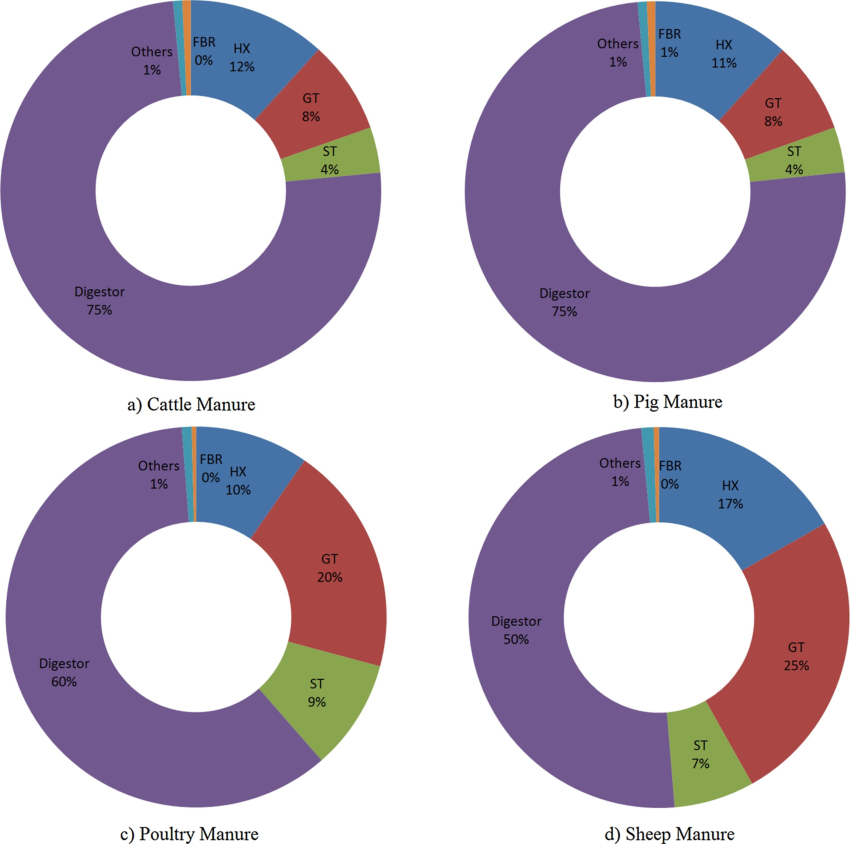
\includegraphics[width=0.8\linewidth, trim={0cm 0cm 0cm 0cm},clip]{gfx/Chapter2/Fig7.pdf} 
	\caption{Units cost distributions for cattle, pig, poultry and sheep manure treatment (ST: steam turbine, GT: gas turbine, HX: heat exchangers, FBR: fluidized bed reactor).}
	\label{fig:CostDist}
\end{figure}

It is clear that the digester shows the largest share in the investment cost and therefore the concentration of the manure highly determines the cost of the facility. \citet{lantz2012economic} presented the investment cost of a facility for heat and power production as a function of its scale. Actually, our plant does not produce steam as a final product but only power. Thus, it is interesting to see that the raw material determines the investment per kW from the 4,000 EUR/kW in case of poultry manure or the 7,500 EUR/kW in case of sheep manure, to the more than 25,000 EUR/kW in case of pig and cattle.

\subsubsection{Production cost}
To calculate the production cost, 20 years of plant life is considered, with a capacity factor of 98\%. Apart from the equipment amortization, other items are also taken into account such as salaries, administrative fees, chemicals cost, maintenance cost, utilities and contingency costs. Thus, apart from the annualized equipment cost, 1.5 M EUR are spent in salaries, 0.25 M EUR in Administration, 2 M EUR in Maintenance, 0.25 M EUR in other expenses \citep{Leon} while chemicals are computed as described in Section \ref{section:ProcessDescription}. The cost of utilities adds up to 0.08 M EUR, accounting for the cooling water and the steam needed to maintain the operation of the digester and to condition the digestate for its use as a fertilizer. Finally, we assume that the livestock manure is for free. Fig. \ref{fig:OpCost} shows the distribution of the production costs for each of the manure types. We see that the figures are very similar. The equipment amortization represents at least 43\% of the production costs. This share increases up to 60\% for the case of the use of poultry. As the investment is lower, the annual cost for other items is almost constant and their contribution to the electricity cost plays a more important role. Chemicals is the second most important contribution to the cost of electricity with a share of up to 23\% for the use of cattle or pig manure and down to 16\% in the case of sheep manure. We assume in all cases that waste is for free. Under these considerations the electricity production costs obtained are presented in Table \ref{table:Table7}.

The Net Profit Value has also been calculated as a measure of the project profitability, considering an electricity price of sale of 0.06 EUR/kWh. To compare the profitability of this project a secure investment as the inversion in Spanish national debt has been chosen, considering a discount rate of 3\% \citep{TesoroSpain}. The results obtained are presented in Table \ref{table:Table7}, and it should be noted that facilities for poultry and sheep manures obtain positive NPV while those which use cattle and pig manure as raw material show negative NPV, so from the point of view of NPV as an indicator to decide the project viability, those ones would be disregarded.



\begin{table}[h!]
	\centering
	\caption{Electricity production cost and NPV for the facility considering different raw materials.}
	\label{table:Table7}
	\resizebox{0.95\columnwidth}{!}{
		\begin{tabular}{@{}cccc@{}}
			\toprule
			Raw material   & \begin{tabular}[c]{@{}c@{}}Annual production costs \\ (M EUR /year)\end{tabular} & \begin{tabular}[c]{@{}c@{}}Electricity production\\ cost (EUR/kWh)\end{tabular} & \begin{tabular}[c]{@{}c@{}}NPV\\ (EUR /year)\end{tabular} \\ \midrule
			Cattle manure  & 12.04                                                                            & 0.45                                                                            & $-1.93 \cdot 10^{7}$                                               \\
			Pig manure     & 12.07                                                                            & 0.45                                                                            & $-1.96\cdot 10^{7}$                                               \\
			Poultry manure & 25.51                                                                            & 0.03                                                                            & $2.85\cdot 10^{8} $                                               \\
			Sheep manure   & 15.53                                                                            & 0.10                                                                            & $5.40\cdot 10^{7} $                                               \\ \bottomrule
		\end{tabular}
	}
\end{table}

\begin{figure}[h!]
	\centering
	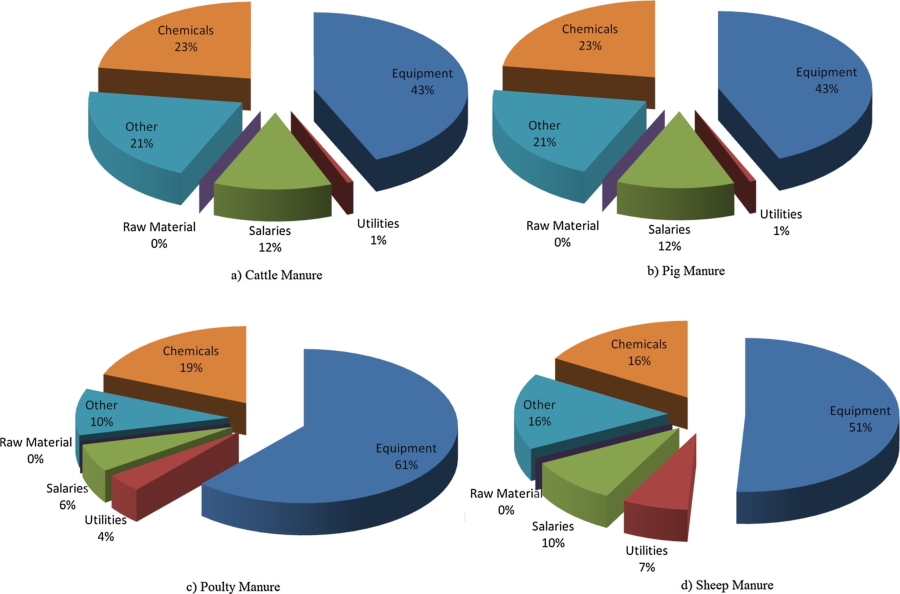
\includegraphics[width=0.9\linewidth, trim={0cm 0cm 0cm 0cm},clip]{gfx/Chapter2/Fig8.pdf} 
	\caption{Operation cost distribution for cattle, pig, poultry and sheep manure treatment.}
	\label{fig:OpCost}
\end{figure}

\subsection{Effect on the power, operating conditions and digestate treatment} \label{section:Effect}
The results obtained from the treatment of different manure streams show the influence of the manure composition in the amount produced and the composition of biogas and digestate obtained. Struvite production using FBR is the best choice for digestate treatment. This can be explained by the advantages in recovering nutrients in solid form since they can be easily transported and stored. Furthermore the material is highly concentrated in nutrients with a relatively high selling price. Biogas production is similar for cattle and pig manures, but is significantly higher in the poultry and sheep cases. The investment cost when processing cattle and pig manure is dominated by the digester, resulting in similar investment and production costs for facilities using either of the two types of manure. However, the higher concentration in organic matter in sheep and poultry manure does not only results in higher power production capacities, but the fact that the contribution to the cost of the turbines is also larger and so is the investment cost of these facilities. On the other hand, the electricity production cost is lower in the last two cases as result of the economies of scale between the investment cost and the biogas produced and the higher amount of struvite produced, with the extreme case of poultry manure where the struvite selling benefits are capable to cover the electricity production costs. Note that the availability of poultry and or sheep manure should be less that than for cattle and pig manure.


\section{Conclusions} \label{section:Conclusions}
In this work, we have designed optimal integrated facilities for the production of biogas-based electrical power and fertilizers from manure. Detailed equation based models for the anaerobic digestion, the Brayton and regenerative Rankine cycles and different technologies for digestate treatment have been developed. To solve the model a two-step procedure has been performed. First, the individual detailed models for each digestate treatment technology are used to formulate a MINLP model aiming at selecting the best configuration for that technology: the best precipitation agent, filter media, etc. In the second step, the best configuration of each technology has been implemented in the entire superstructure. Due to the fact that only one digestate processing technology is allowed and the highly non-linear nature of the model, surrogate models for the cost of each alternatives with a smooth approximations have been developed. For the optimal selection a detailed economic evaluation is performed. The results show that FBR technologies are preferred to recovery nutrients. Furthermore, in some cases this process can produce electricity at a competitive price (in case of poultry and sheep manure). The investment cost is highly dependent on the water and organic content of the manure type, ranging from 70 M EUR to 208 M EUR when a large energy production is possible and large gas and steam turbines are to be installed. However, for these cases of higher investment cost, the production cost of power is the most competitive due to the large production capacity. Biogas power plants show a wide range of values of power
per kW installed depending on the manure concentration. Competitive values of 4,000 EUR/kW for poultry manure are obtained, due to the highly concentrated manure, while large values of 25,000 EUR/kW installed are reported in case of the diluted cattle or pig manure.


\section*{Nomenclature}
\addcontentsline{toc}{section}{Nomenclature}

\vspace{-0.8cm}
\begingroup     
\let\clearpage\relax
%
 \newglossaryentry{set1}{type=SetsCh2,name={i},description={$\in \left\{ \text{P, N} \right\}$}}
 \newglossaryentry{set2}{type=SetsCh2,name={j},description={$\in \left\{ \text{filter media} \right\}$}}
 \newglossaryentry{set3}{type=SetsCh2,name={k},description={$\in \left\{ \text{TS, C, K} \right\}$}}
 \newglossaryentry{set4}{type=SetsCh2,name={a'},description={$\in \left\{\text{CH\textsubscript{4},  CO\textsubscript{2}, NH\textsubscript{3}, H\textsubscript{2}S, O\textsubscript{2}, N\textsubscript{2}}\right\}$}}
 \newglossaryentry{set5}{type=SetsCh2,name={a},description={$\in \left\{ \text{H\textsubscript{2}O, CH\textsubscript{4}, CO\textsubscript{2}, NH\textsubscript3, H\textsubscript{2}S, O\textsubscript{2}, N\textsubscript{2}} \right\}$}}
 \newglossaryentry{set6}{type=SetsCh2,name={d},description={$\in \left\{ \text{C, N\textsubscript{organic}, N\textsubscript{NH\textsubscript{3}}, P, K, H\textsubscript{2}O, Rest} \right\}$}}
 \newglossaryentry{set7}{type=SetsCh2,name={e},description={$\in \left\{ \text{CH\textsubscript{4}, NH\textsubscript{3}, H\textsubscript{2}S} \right\}$}}
 \newglossaryentry{set8}{type=SetsCh2,name={h},description={$\in \left\{ \text{CH\textsubscript{4}, CO\textsubscript{2}, O\textsubscript{2}, N\textsubscript{2}} \right\}$}}
 %
 \newglossaryentry{param1}{type=ParamCh2,name={$A_{specific}$},description={specific clarifier area (m\textsuperscript{2}/(ton·day))}}
 \newglossaryentry{param2}{type=ParamCh2,name={$A(i)$},description={Antoine $A$ coefficient for vapor pressure of component $i$}}
 \newglossaryentry{param3}{type=ParamCh2,name={$B(i)$},description={Antoine $B$ coefficient for vapor pressure of component $i$}}
 \newglossaryentry{param4}{type=ParamCh2,name={$C(i)$},description={Antoine $C$ coefficient for vapor pressure of component $i$}}
 \newglossaryentry{param5}{type=ParamCh2,name={$c_{p_{sat}}$},description={specific heat capacity of flue gas}}
 \newglossaryentry{param6}{type=ParamCh2,name={$d$},description={working days per year}}
 \newglossaryentry{param7}{type=ParamCh2,name={$d_{p}$},description={particle diameter (m)}}
 \newglossaryentry{param8}{type=ParamCh2,name={$k$},description={kinetic constant $\left( \text{s}^{-1}\right) $}}
 \newglossaryentry{param9}{type=ParamCh2,name={$IAP_{eq}$},description={ion activity product equilibrium}}
 \newglossaryentry{param10}{type=ParamCh2,name={$h$},description={working hours per day}}
 \newglossaryentry{param11}{type=ParamCh2,name={$HRT_{unit}$},description={hydraulic retention time of $unit$ (s)}}
 \newglossaryentry{param12}{type=ParamCh2,name={$MW_{component}$},description={molecular weight of $component$ (kg/kmol)}}
 \newglossaryentry{param13}{type=ParamCh2,name={$MeP_{ratio}$},description={metal/phosphorus molar ratio in coagulation process}}
 \newglossaryentry{param14}{type=ParamCh2,name={$Price_{component}$},description={price of $component$ (EUR/kg)}}
 \newglossaryentry{param15}{type=ParamCh2,name={$g$},description={gravity acceleration $\left(\text{m}^{2} / \text{s} \right)$}}
 \newglossaryentry{param16}{type=ParamCh2,name={$\kappa_{agitator}$},description={agitator specific power consumed (HP/1000 US gallon)}}
 \newglossaryentry{param17}{type=ParamCh2,name={$\varphi_j$},description={precipitation agent $j$ : total solids (mass ratio)}}
 \newglossaryentry{param18}{type=ParamCh2,name={$\eta_c$},description={compressors efficiency (0.85)}}
 \newglossaryentry{param19}{type=ParamCh2,name={$\eta_s$},description={isentropic efficiency (0.9)}}
 \newglossaryentry{param20}{type=ParamCh2,name={$\eta_i^j$},description={separation yield of componente $i$ in inprocess $j$}}
 \newglossaryentry{param21}{type=ParamCh2,name={$P_{atm}$},description={atmospheric pressure (1 bar)}}
 \newglossaryentry{param22}{type=ParamCh2,name={$T_{atm}$},description={room temperature (25 ºC)}}
 \newglossaryentry{param23}{type=ParamCh2,name={$R$},description={ideal gas constant (8.314 J/mol·K)}}
 \newglossaryentry{param24}{type=ParamCh2,name={$c_{p_{H_{2}O}}$},description={specific heat capacity of water (4.18 kJ/kg \textdegree C)}}
 %
 \newglossaryentry{var1}{type=VarCh2,name={$a_{technology}$},description={selection parameter which takes value 0 when $F_{design}^{technology}$is 0 and 1 if $F_{design}^{technology}$ is not equal to 0}}
 \newglossaryentry{var2}{type=VarCh2,name={$\alpha_{mf}$},description={parameter dependent of the number of phases in the FBR}}
 \newglossaryentry{var3}{type=VarCh2,name={$Ar_l$},description={Arquimedes number for liquid}}
 \newglossaryentry{var4}{type=VarCh2,name={$A_unit$},description={area of unit $\left( \text{m}^2 \right)$}}
 \newglossaryentry{var5}{type=VarCh2,name={$Benefits_{technology}$},description={benefits or losses obtained with $technology$}}
 \newglossaryentry{var6}{type=VarCh2,name={$C:N$},description={carbon to nitrogen molar ratio}}
 \newglossaryentry{var7}{type=VarCh2,name={$C_{eq}$},description={equilibrium concentration (kmol/m\textsuperscript{3})}}
 \newglossaryentry{var8}{type=VarCh2,name={$C_0$},description={initial concentration (kmol/m\textsuperscript{3})}}
 \newglossaryentry{var9}{type=VarCh2,name={$Cost_{unit}$},description={cost of $unit$}}
 \newglossaryentry{var10}{type=VarCh2,name={$C_{component}^{unit}$},description={concentration of $component$ in the $unit$ inlet stream $\left(\text{kg\textsubscript{component}} / \text{kg\textsubscript{total}} \right) $}}
 \newglossaryentry{var11}{type=VarCh2,name={$ChemC_technology$},description={cost of chemicals for $technology$}}
 \newglossaryentry{var12}{type=VarCh2,name={$D_{unit}$},description={diameter of $unit$}}
 \newglossaryentry{var13}{type=VarCh2,name={$e_{unit}$},description={thickness of $unit$}}
 \newglossaryentry{var14}{type=VarCh2,name={$Ec_{j}\left( T \right)$},description={equilibrium constant of component $j$ at temperature T}}
 \newglossaryentry{var15}{type=VarCh2,name={$F_{component}^{unit}$},description={mass flow of $component$ in the $unit$ inlet stream (kg/s)}}
 \newglossaryentry{var16}{type=VarCh2,name={$F_{max}^{unit}$},description={maximum mass inlet flow admitted by a single unit (kg/s)}}
 \newglossaryentry{var17}{type=VarCh2,name={$F_{design}^{unit}$},description={mass inlet flow used in the design of $unit$ (kg/s)}}
 \newglossaryentry{var18}{type=VarCh2,name={$FC_{technology}$},description={fixed cost of $technology$}}
 \newglossaryentry{var19}{type=VarCh2,name={$F_{total}^{recovered}$},description={recovered matter total mass flow (kg/s)}}
 \newglossaryentry{var20}{type=VarCh2,name={$F^{unit,unit1}$},description={mass flow from stream from $unit$ to $unit1$ (kg/s)}}
 \newglossaryentry{var21}{type=VarCh2,name={$fc_{j}^{unit,unit1}$},description={mass flow of component $j$ from $unit$ to $unit1$ (kg/s)}}
 \newglossaryentry{var22}{type=VarCh2,name={$H_{b}^{unit,unit1)}$},description={enthalpy of the stream at state b from $unit$ to $unit1$ (kJ/kg)}}
 \newglossaryentry{var23}{type=VarCh2,name={$H_{steam (isoentropy)}$},description={isentropic expansion enthalpy of steam (kJ/kg)}}
 \newglossaryentry{var24}{type=VarCh2,name={$l_{j-i}$},description={molar fraction of component $j$ in the liquid phase of equilibrium system $i$}}
 \newglossaryentry{var25}{type=VarCh2,name={$K_{index}$},description={potassium index of fertilizer}}
 \newglossaryentry{var26}{type=VarCh2,name={$L_{unit}$},description={length of $unit$}}
 \newglossaryentry{var27}{type=VarCh2,name={$N_{NH_{3}}$},description={nitrogen contained in ammonia}}
 \newglossaryentry{var28}{type=VarCh2,name={$N_{org}$},description={nitrogen contained in organic matter}}
 \newglossaryentry{var29}{type=VarCh2,name={$n_{unit}$},description={number of units used in the process}}
 \newglossaryentry{var30}{type=VarCh2,name={$n_{(unit,unit1)}$},description={total mol flow from stream from $unit$ to $unit1$ (kmol/s)}}
 \newglossaryentry{var31}{type=VarCh2,name={$N_{index}$},description={nitrogen index of fertilizer}}
 \newglossaryentry{var32}{type=VarCh2,name={$P_{in/compressor}$},description={inlet pressure to compressor (bar)}}
 \newglossaryentry{var33}{type=VarCh2,name={$P_{out/compressor}$},description={outlet pressure of compressor (bar)}}
 \newglossaryentry{var34}{type=VarCh2,name={$P_j^{*} \left( T \right)$},description={saturation pressure of pure component $j$ at temperature T (bar)}}
 \newglossaryentry{var35}{type=VarCh2,name={$P_v$},description={vapor pressure (bar)}}
 \newglossaryentry{var36}{type=VarCh2,name={$P_{index}$},description={phosphorous index of fertilizer}}
 \newglossaryentry{var37}{type=VarCh2,name={$p_{turb,i}$},description={inlet pressure to body $i$ in the turbine (bar)}}
 \newglossaryentry{var38}{type=VarCh2,name={$P_{unit}$},description={power of unit}}
 \newglossaryentry{var39}{type=VarCh2,name={$Q_{(unit)}$},description={heat exchanged in $unit$ (kW)}}
 \newglossaryentry{var40}{type=VarCh2,name={$R_{C-N/k}$},description={carbon to nitrogen ratio in $k$}}
 \newglossaryentry{var41}{type=VarCh2,name={$R_{C-N/fertilizer}$},description={carbon to nitrogen ratio in fertilizer}}
 \newglossaryentry{var42}{type=VarCh2,name={$R_{V-F/i}$},description={rate of evaporation in equilibrium system $i$}}
 \newglossaryentry{var43}{type=VarCh2,name={$Rest$},description={rest of the elements contained in the biomass}}
 \newglossaryentry{var44}{type=VarCh2,name={$Re_{l,mf}$},description={Reynolds number for liquid in minimum fluidization conditions}}
 \newglossaryentry{var45}{type=VarCh2,name={$s_{b,(unit,unit1)}$},description={entropy the stream at the state $b$ for the stream from $unit$ to $unit1$ (kJ/kg·K)}}
 \newglossaryentry{var46}{type=VarCh2,name={$T_{turb,i, min}^{*}$},description={saturated temperature at exit of body $i$ (\textdegree C)}}
 \newglossaryentry{var47}{type=VarCh2,name={$T_{(unit,unit1)}$},description={temperature of the stream from $unit$ to $unit1$ (\textdegree C)}}
 \newglossaryentry{var48}{type=VarCh2,name={$T_{bubble/i}$},description={bubble point temperature of equilibrium system $i$ (\textdegree C)}}
 \newglossaryentry{var49}{type=VarCh2,name={$T_{m/i}$},description={average temperature in equilibrium system $i$ (\textdegree C)}}
 \newglossaryentry{var50}{type=VarCh2,name={$T_{in/compressor}$},description={inlet temperature to compressor (\textdegree C)}}
 \newglossaryentry{var51}{type=VarCh2,name={$T_{out/compressor}$},description={outlet temperature of compressor (\textdegree C)}}
 \newglossaryentry{var52}{type=VarCh2,name={$t$},description={time (s)}}
 \newglossaryentry{var53}{type=VarCh2,name={$u_t$},description={terminal velocity (m/s)}}
 \newglossaryentry{var54}{type=VarCh2,name={$u_0$},description={fluid velocity (m/s)}}
 \newglossaryentry{var55}{type=VarCh2,name={$u_{mf}$},description={minimum fluidization velocity (m/s)}}
 \newglossaryentry{var56}{type=VarCh2,name={$v_{j-i}$},description={molar fraction of component $j$ in the vapor phase of equilibrium system $i$}}
 \newglossaryentry{var57}{type=VarCh2,name={$V_{biogas,k}$},description={biogas volume produced per unit of volatile solids (VS) associated to waste $k$ (m\textsuperscript{3}\textsubscript{biogas}/kg\textsubscript{VS/k})}}
 \newglossaryentry{var58}{type=VarCh2,name={$V_{unit}$},description={volume of $unit$}}
 \newglossaryentry{var59}{type=VarCh2,name={$W_{unit}$},description={weight of $unit$}}
 \newglossaryentry{var60}{type=VarCh2,name={$w^\prime_{DM/k}$},description={dry mass fraction of $k$ (kg\textsubscript{DM/k}/kg)}}
 \newglossaryentry{var61}{type=VarCh2,name={$w^\prime_{VS/k}$},description={dry mass fraction of volatile solids out of the dry mass of $k$ (kg\textsubscript{VS/k}/kg\textsubscript{DM/k})}}
 \newglossaryentry{var62}{type=VarCh2,name={$w^\prime_{C/k}$},description={dry mass fraction of C in $k$ (kg\textsubscript{C/k}/kg\textsubscript{DM/k})}}
 \newglossaryentry{var63}{type=VarCh2,name={$w^\prime_{NH_{3}/k}$},description={dry mass fraction of NH\textsubscript{3} in $k$ (kg\textsubscript{NH\textsubscript{3}/k}/kg\textsubscript{DM/k})}}
 \newglossaryentry{var64}{type=VarCh2,name={$w^\prime_{N_{org}/k}$},description={dry mass fraction of N\textsubscript{org} in $k$ (kg\textsubscript{N\textsubscript{org}/k}/kg\textsubscript{DM/k})}}
 \newglossaryentry{var65}{type=VarCh2,name={$w^\prime_{P/k}$},description={dry mass fraction of P in $k$ (kg\textsubscript{P/k}/\textsubscript{DM/k})}}
 \newglossaryentry{var66}{type=VarCh2,name={$w^\prime_{K/k}$},description={dry mass fraction of K in $k$ (kg\textsubscript{K/k}/\textsubscript{DM/k})}}
 \newglossaryentry{var67}{type=VarCh2,name={$w^\prime_{Rest/k}$},description={dry mass fraction of the rest of the elements contained in $k$ (kg\textsubscript{Rest/k}/kg\textsubscript{DM/k})}}
 \newglossaryentry{var68}{type=VarCh2,name={$W_{unit}$},description={power produced or consumed in $unit$ (kW)}}
 \newglossaryentry{var69}{type=VarCh2,name={$w^\prime_{Rest/k}$},description={dry mass fraction of the rest of the elements contained in $k$ (kg\textsubscript{Rest/k}/kg\textsubscript{DM/k})}}
 \newglossaryentry{var70}{type=VarCh2,name={$x_{a/biogas}$},description={mass fraction of component $a$ in the biogas}}
 \newglossaryentry{var71}{type=VarCh2,name={$y^j$},description={binary variable to evaluate the element $j$}}
 \newglossaryentry{var72}{type=VarCh2,name={$y_{biogas}$},description={specific saturated moisture of biogas}}
 \newglossaryentry{var73}{type=VarCh2,name={$w^\prime_{Rest/k}$},description={dry mass fraction of the rest of the elements contained in $k$ (kg\textsubscript{Rest/k}/kg\textsubscript{DM/k})}}
 \newglossaryentry{var74}{type=VarCh2,name={$Y_{a', biogas-dry}$},description={molar fraction of component a in the dry biogas}}
 \newglossaryentry{var75}{type=VarCh2,name={$\Delta H_{reaction(bioreactor)}$},description={reaction heat of anaerobic digestion (kW)}}
 \newglossaryentry{var76}{type=VarCh2,name={$\Delta H_{comb, k}$},description={heat of combustion of component $k$ (kW)}}
 \newglossaryentry{var77}{type=VarCh2,name={$\Delta H_{comb, e}$},description={heat of combustion of component $e$ (kW)}}
 \newglossaryentry{var78}{type=VarCh2,name={$\Delta H_{comb, digestate-dry}$},description={heat of combustion of dry digestate (kW)}}
 \newglossaryentry{var79}{type=VarCh2,name={$\Delta H_{f, h} \left( T \right) $},description={heat of formation of component $h$ at temperature T (kW)}}
 \newglossaryentry{var80}{type=VarCh2,name={$Z$},description={objective function}}
 \newglossaryentry{var81}{type=VarCh2,name={$\rho_{component}$},description={density of $component$ (kg/m\textsuperscript{3})}}
 \newglossaryentry{var82}{type=VarCh2,name={$\mu_{component}$},description={viscosity of component (kg/(m·s))}}

%
\glsaddall
%**************************************************************
%This is for horizontal spacing between acronym and description
\setlength\LTleft{0pt}
\setlength\LTright{0pt}
\setlength\glsdescwidth{0.8\hsize}
%**************************************************************
%**************************************************************
%This is for vertical spacing between title and entries
\renewcommand*{\glossarypreamble}{\vspace{-0.8cm}}
%**************************************************************
\printglossary[type=SetsCh2, style=long]
\vspace{10pt}
\printglossary[type=ParamCh2, style=long]
\vspace{10pt}
\printglossary[type=VarCh2, style=long]
%\printglossaries
\endgroup

\section*{Acknowledgments} \label{section:Acknowledgments}
\addcontentsline{toc}{section}{Acknowledgments}
We acknowledge funding from the National Science Foundation (under grant CBET-1604374) and MINECO (under grant DPI2015-67341-C2-1-R) and E.M. also acknowledges an undergraduate research grant.

\section*{Bibliography}
\addcontentsline{toc}{section}{Bibliography}

\printbibliography[heading=none]
\end{refsection}
%\printbibliography[heading=none]

%\cleardoublepage%*****************************************
\chapter{Assessment of phosphorus recovery through struvite precipitation}\label{ch:Struvite}
%*****************************************
\begin{refsection}[referencesCh3]
\section{Introduction}
Livestock farming and other agricultural activities have altered the natural nutrient cycles. Phosphorus, one of the three plant-grow macronutrients, enters to the global cycle as phosphate rock, which through erosion and chemical weathering is transferred to soils and waterbodies. Also, phosphorus deposited in soils will reach fresh and marine waterbodies by runoff. Phosphorus in rivers is transported to stagnant waterbodies (such as lakes) and oceans, reaching the bottom of lakes and oceans as sediments. The cycle is closed when the buried phosphorus is uplifted again by tectonic processes. Along the cycle, phosphorus can be taken by plants and algae, but after the death of living organisms it returns to the cycle \citep{RUTTENBERG2001401}. This global natural cycle is largely altered by human activities through the mining and shipping of phosphate rock, mainly for fertilizer production, resulting in unbalanced phosphorus releases to the environment.

Nutrient pollution from anthropogenic sources has become as a critical worldwide water quality problems. Nutrient contamination results in environmental and public health issues as a result of the exponential growth of algae, cyanobacteria, and the occurrence of harmful algal blooms (HABs), which turns into dead zones and hypoxia due to the aerobic degradation of the algal biomass by bacteria; shifting the distribution of aquatic species and releasing toxins in drinking water \citep{Sampat2}. In addition, the development of HABs and eutrophication processes contributes to climate change through the emission of large amounts of strong greenhouse gases such as $\text{CH}_{4}$ and $\text{N}_{2}\text{O}$ \citep{Beaulieu}.

However, phosphorus is a limited non-renewable resource, essential nutrient to support life, and widely used as fertilizer to increase crop yields. Actually, phosphorus is one of the most sensitive elements to depletion, as it is a key agricultural fertilizer that has no known substitute. Current global reserves of phosphate rock could be depleted in the next 50 to 100 years \citep{Cordell}. Therefore, the development of a circular economy around phosphorus capable of recovering the nutrient and reintegrating it into the productive cycle is not only desirable but also a necessary measure to reach sustainable development. Agricultural activities are the main source of nutrients in waterbodies \citep{Dzombak}, and among them, livestock industry is one of the largest economic sectors. Additionally, the increasing income-spending potential of the middle class in developing countries has increased the demand for dairy and beef products, resulting in the generation of large amounts of livestock organic waste. Considering that an average dairy cow generates 51.19 kg of raw manure per day \citep{USDAWaste}, the total phosphorus excreted is 11.02 kg per year per animal, equivalent to 5.96 kg of phosphorus as phosphate per year per animal. In the U.S. as of January 2020, a total of 94.4 million head has been reported \citep{USDACattle2020}. Thus, this shows potential phosphate U.S. releases of $562.6\cdot10^{6}$ kg/yr. \citet{Sampat} presented the link between the presence of livestock facilities and larger concentrations of phosphorus in soil, which potentially can be lost as runoff reaching waterbodies. 
For animals on pasture, organic waste should not be a resource of concern if stocking rates are not excessive. However, for concentrate animal feeding operations (CAFOs), manure should be correctly managed due to the high rates and spatial concentration of the organic waste generated, representing potential environmental issues. Usually, manure is collected in the animal living zones, and stored as liquid or slurry to be further spread in croplands as nutrient supplementation; or as solid in dry stacking or composting facilities to be sold as compost. Liquid fraction of manure can be also treated in aerobic or anaerobic ponds. However, these approaches do not allow a correct nutrient management since nutrients concentration is variable and not well defined, and nitrogen and phosphorus are unbalanced regarding the nutrient necessities of plans, i.e., if nitrogen demand is covered, there is a surplus in the phosphorus supply which can runoff to waterbodies, and if phosphorus demand is covered, there is a deficit in the nitrogen supply, being necessary to apply additional fertilizers. In addition, during rainy periods the applied manure can runoff, dragging the nutrients contained in it. Nonetheless, phosphorus from liquid cattle waste, either processed in an anaerobic digestion stage or raw waste, can be potentially recovered through different processes \citep{muhmood2019formation}, reducing the nutrient inputs to waterbodies and its consequential environmental, economic, and social impacts. Among these, it is found that struvite production is one of the most promising cost-effective choices for the recovery of nutrients from cattle waste \citep{Martin}. Struvite is a phosphate-based mineral, which can be applied as a slow release fertilizer \citep{Richards}, allowing the redistribution of phosphorus from livestock facilities to nutrient-deficient locations.

Previous studies report struvite formation from different sources of waste, such as municipal wastewater treatment plants \citep{Battistoni}, mineral fertilizer industry \citep{Matynia}, or agricultural industry \citep{Shashvatt}. Thermodynamic models representing the formation of struvite and other precipitates have been also developed for various wastes including liquid swine manure \citep{celen_using_2007}, human urine \citep{Harada, ronteltap_struvite_2007}, and municipal wastewater \citep{rahaman_modeling_2014}. Additionally, some complex approaches considering the hydrodynamic and kinetic effects in the formation of struvite have been studied but limited to wastewater treatment \citep{rahaman_modeling_2014, mangin2004fluid}. However, the results obtained from those studies cannot be extrapolated to struvite formation from cattle organic waste, since these residues have some characteristics that hinder struvite formation, including high ionic strength, which reduces the effective concentration of ions; the presence of calcium ions competing for phosphate ions \citep{Yan}, which inhibits a selective recovery by nutrient precipitation techniques; and the high variability in the manure composition, as a function of the geographical area, the animal feed, etc. \citep{Tao}. Other controlling factors are the pH level, the magnesium-phosphorus ratio, and the alkalinity of the leachate. Therefore, for an accurate prediction of struvite formation from this waste, it is necessary to include within the thermodynamic model structure for precipitates formation the specific features  of cattle waste described above.

In this work, specific surrogate models to predict the production of struvite and calcium precipitates from cattle leachate are developed based on a detailed and robust thermodynamic model. In addition, the variability in the organic waste composition is captured through a probability framework based on Monte Carlo method. The reduced models obtained are used to evaluate the potential of struvite production from cattle waste to mitigate phosphorus releases in watersheds of the United States. Future applications of the developed surrogate models include the development of applications for environmental assessment and the design of policies to prevent nutrient releases, among others.

\section{Methods}
\subsection{Spatial resolution}
A watershed is an area of land which drains all the streams and rainfall to a common drainage, defining the spatial boundaries for the collection of lost elements as runoff. The surface  water  drainages of the U.S. are identified by the U.S. Geological Survey through the Hydrologic Unit Code system (HUC). The HUC system is a hierarchical system indicated by the number of digits in groups of two, with six levels identified by codes from 2 to 12 digits (i.e., HUC2 to HUC12). These levels refer to regions, subregions, basins, subbasins, watersheds, and subwatersheds. The spatial resolution of this study is the continental United States at watershed scale, considering the boundaries defined by the Hydrologic Unit Code system at 8 digits (HUC8), representing the subbasin level \citep{HUC8}.

\subsection{Assessment of anthropogenic phosphorus from agricultural activities}
\subsubsection{Phosphorus releases} \label{Preleases}
Agricultural emissions are one of the main sources of anthropogenic P releases due to the excessive use of commercial fertilizers and livestock manure for cropland nutrients needs and the uncontrolled nutrient runoff to waterbodies, although for some areas urban source releases can contribute significantly to the total P releases to the environment. However, this analysis is limited to the evaluation of phosphorus releases from agricultural activities \citep{Dzombak, Alexander_2008, SPARROW_report_1999}.

Watershed phosphorus releases $\left(E_{x}\right)$ are computed as the sum of the phosphorus releases from fertilizer applications to croplands and from the manure generated by livestock facilities. The releases of phosphorus to each watershed by manure emissions, accounting cattle, swine and poultry, and by fertilizers application, is reported by the IPNI NuGIS project. This is consitent with the most recent data available (year 2014) for fertilizers sales provided by the Association of American Plant Food Control Officials (AAPFCO), fitting the data to HUC8 watershed boundaries. More information about the methodology used for the estimation of agricultural phosphorus releases can be found in \citep{NuGIS}. Phosphorus content for several commercial phosphate fertilizers and different manure types can be found in \citet{OSU2017} and \citet{OSU2005} respectively.

\subsubsection{Phosphorus uptakes}
The elements considered for phosphorus uptake are the crops sown and managed by humans in each watershed. Additionally, the phosphorus retained by wetlands has been considered in the phosphorus balance. The phosphorus uptake by each type of vegetation at watershed level is computed as the product of the land area occupied, the grow yields per area unit and the phosphorus uptake per plant mass unit. Therefore, the total watershed phosphorus uptake $\left(U_{x}\right)$ is computed as the sum of the phosphorus uptake by each type of plant, Eq. \ref{eq:U_x}.

\begin{align}
%& U_{i} = \text{Area}_{i} \cdot \text{Yield}_{i} \cdot \text{P}_{\text{uptake }i} \ \forall \ i \ \in \ {\text{Plant varieties}} \label{eq:U_i} \\
& U_{x} = \sum^{i} \text{Area}_{i} \cdot \text{Yield}_{i} \cdot \text{P}_{\text{uptake }i} \ \forall \ i \ \in \ {\text{Plant varieties}} \label{eq:U_x}
\end{align}
Since different crops have different phosphorus uptakes and yield rates, the amount of each type of crop is estimated for each watershed. To determine the land cover uses, accounting croplands, pasturelands, wetlands and developed areas (urban areas), information available for the most recent year (2011) from the U.S. Environmental Protection Agency's (U.S. EPA) EnviroAtlas database is used \citep{EnviroAtlas}. Data from EnviroAtlas is provided with higher spatial resolution, at HUC12 level. To ensure spatial consistency, the data is reconciled at HUC8 level. Once the land uses of each watershed are known, data from the 2017 U.S. Census of Agriculture is used to determine the distribution of crops on croplands, considering corn, soybeans, small grains, cotton, rice, vegetables, orchards, greenhouse and other crops (namely oil crops, sugar crops, and fruits) \citep{2017CensusofAgriculture}. The data provided by the U.S. Census of Agriculture have a spatial resolution of HUC6. Therefore, it is reconciled at HUC8 level scaling by the area fraction represented by each HUC8 watershed over the total HUC6 hydrologic unit. If two or more crops were harvested from the same land during the year (double cropping), the area was counted for each crop. To determine the nutrients uptake of each type of crop, data from the U.S. Department of Agriculture (USDA) Waste Management field Handbook is considered  \citep{USDAWaste}. For croplands, the specific nutrient uptake values are used for corn, soybeans, cotton, rice and orchards, while average values including the most representative species are used for small grains, vegetables, greenhouse crops, pasture crops, and forest. For pasture lands the average nutrient uptake and crop yield including the main pasture crops: alfalfa, switchgrass and wheatgrass; for forests lands the nutrient uptake and crop yield of Northern hardwoods is considered, and for developed areas null nutrient uptake is considered. The wetlands phosphorus uptake value considered is 0.77 gP m$^{-2}$ year$^{-1}$, based in the data reported by \citet{Kadlec}.

\subsubsection{Phosphorus balance}
To reach environmental sustainability of a productive activity, the releases of phosphorus should be balanced with the phosphorus uptakes from that activity, reducing the impact over the original ecosystems as much as possible. To evaluate the balance of phosphorus releases involved in agricultural activities throughout the U.S. watersheds, the techno-ecological synergy (TES) sustainability metric proposed by \citet{TESmetric} has been considered, Eq. \ref{eq:TES}. A negative value of $V_{x}$ indicates that the emissions, $\left(E_{x}\right)$, are larger than the uptake capacity of the agricultural activities, $\left(U_{x}\right)$, impacting the ecosystems, while positive values reflect that the releases are lower than the uptake capacity.

\begin{align}
& V_{x} =\frac{\left(U_{x} - E_{x}\right)}{E_{x}} \label{eq:TES}
\end{align}

\subsection{Thermodynamic model for precipitates formation} \label{thermo_model}
The behavior of cattle leachate system has been evaluated through a thermodynamic model, evaluating the formation of different precipitates through chemical equilibrium and material balances, capturing the mutual dependencies based on the competition for the same ions. Four aqueous chemical systems have been considered, water, ammonium, phosphoric acid, and carbonates systems. Moreover, the formation of seven possible precipitates is evaluated: struvite, K-struvite, magnesium hydroxide, calcium hydroxide, calcium carbonate, hydroxyapatite, dicalcium phosphate, and tricalcium phosphate.

\subsubsection{Uncertainty in livestock organic waste composition} \label{comp_dist}
The variability in the composition of raw material creates operational difficulties that any material recovery process must deal with. The composition of cattle organic waste depends on multiple factors, among which are livestock feed, geographical area, climate, and other local factors of the livestock operation \citep{Tao}. Several elements of cattle manure composition play an active role in the formation of struvite and other precipitates. These include the high ionic strength, which reduces the effective concentration of ions; and the distribution ratios between calcium, ammonia and phosphate; and the leachate alkalinity, affecting the chemical equilibrium. To capture the uncertainty generated by the variability in the composition of cattle leachate, 37 data sets of 20 literature references containing the mass fraction of different elements comprising organic livestock waste are evaluated. To estimate feasible cattle leachate compositions, the probability density distribution of each element is calculated by fitting it to the kernel density estimate (KDEs). The selected probability density distributions are normal distribution, as shown in Eq. \ref{eq:normal_dist}, for the distribution of nitrogen, nitrogen as ammonia/total nitrogen ratio, and phosphorus; and lognormal distribution, as defined by  Eq. \ref{eq:lognormal_dist}, for phosphorus as phosphate/total phosphorus ratio, calcium, and potassium. The probability density distribution parameters for each evaluated compound are collected in Table \ref{table:PDD_paramenters}, where $\sigma$ is the standard deviation, $\sigma^2$ is the variance, $\mu$ is the mean of the distribution, $M$ is equal to $e^{\mu}$, and $\gamma$ is a displacement parameter. Kernel density estimations and probability density distributions for each element evaluated can be found in the Supplementary Material. 

The uncertainty in the composition of cattle waste is addressed through the evaluation of the thermodynamic model described in the following sections for multiple cattle waste compositions generated including the probability density distribution of each elements in a Monte Carlo model \citep{Thomopoulos}.

\begin{align}
f(x) = \frac{1}{\sqrt{2 \pi \sigma}}e^{- \frac{\left( x - \mu \right)^{2}}{2 \sigma ^ {2}}} & \label{eq:normal_dist} \\
f(x) = \frac{\frac{1}{\frac{x- \gamma}{M} \sigma \sqrt{2 \pi}} e^{-\frac{ln\left( \frac{x- \gamma}{M} \right)^{2}}{2 \sigma^{2}}}}{M} \label{eq:lognormal_dist}
\end{align}

\begin{table}[h] 
	\centering
	\caption{Probability density distributions parameters for cattle organic waste elements.} \label{table:PDD_paramenters}
	\resizebox{\columnwidth}{!}{
	\begin{tabular}{c c c c c c c c} %llrll
		\toprule
		\multicolumn{1}{c}{Param.}&\multicolumn{3}{c}{Normal distribution}&\multicolumn{1}{c}{Param.}&\multicolumn{3}{c}{Lognormal distribution} \\ \cmidrule(lr){2-4}\cmidrule(lr){6-8}%\hline 
		\\[-1em]
		&N		&$\text{N-NH}^{+}_{4}:\text{N}_{\text{total}}$		&P	&		&$\text{P-PO}_{4}^{3-}:\text{P}_{\text{total}}$		&$\text{Ca}$		&$\text{K}$ 		\\ \midrule
		$\mu$		&0.3841			&0.6200			&0.04000	&$M$		&42.15		&0.08000	&0.2600			\\ 
		$\sigma$	&0.1309			&0.1250			&0.03684	&$\sigma$		&0.0040		&0.4500		&0.8000		\\ 
		&				&				&			&$\gamma$		&-41.53		&0.04044	&0.03389		\\ 
		\bottomrule
	\end{tabular}
	}
\end{table}

\subsubsection{Initial conditions} \label{Initial parameters}
A set of initial conditions must be defined to establish the physico-chemical characteristics of the livestock organic material \citep{Tao}, see Table \ref{table:init_cond}. Please note that pH refers the adjusted pH for optimal struvite precipitation \citep{Tao, Zeng}. 

\begin{table}[h]
	\centering
	\caption{Initial conditions of the livestock organic material system} \label{table:init_cond}.
	\begin{tabular}{@{}ccc@{}}
		\toprule
		Variable               & Value                                                                                      & Unit                               \\ \midrule
		Temperature             & 298                                                                                        & K                                  \\
		pH                      & 9                                                                                          & -                                  \\
		Electrical conductivity ($EC$) & 18,800                                                                                     & $\frac{\mu \text{S}}{\text{cm}}$\\
		Alkalinity              & 3000-14500                                                                                 & mg of CaCO$_{3}$                        \\
		{[Ca$^{2+}$]}               & \begin{tabular}[c]{@{}c@{}} 0.075-0.175 \\ (determined by Monte Carlo model) \end{tabular}											& \% wt wet                          \\
		{[K$^{+}$]}                       & \begin{tabular}[c]{@{}c@{}} 0.10-0.65 \\ (determined by Monte Carlo model) \end{tabular}     & \% wt wet                          \\
		{[P-PO$_{4}^{3-}$]}                      & \begin{tabular}[c]{@{}c@{}} 0.001-0.024 \\ (determined by Monte Carlo model) \end{tabular} & \% wt wet                          \\
		{[N-NH$_{4}^{+}$]}                      & \begin{tabular}[c]{@{}c@{}} 0.015-0.64 \\ (determined by Monte Carlo model) \end{tabular}  & \% wt wet                          \\
		{[Mg$^{2+}$]}                      &  0-10                                                                                       &$\text{Mg}^{2+}/\text{PO}_{4}^{3-}$ molar ratio           \\ \bottomrule
	\end{tabular}
\end{table}

\subsubsection{Activities} \label{Activity coefficients}
Since the cattle waste is a highly non-ideal media due to the high concentrations of dissolved ions, activities instead of molar concentrations are used in the model. Activity coefficients $\left(\gamma_{x}\right)$ for a element $x$ are calculated using the Debye-H\"{u}ckel relationship, Eq. \ref{eq:act_coef}, which relates activity coefficient, temperature, and ionic strength, calculated using Eq. \ref{eq:I}. Eq. \ref{eq:A} is employed to estimate the parameter $A$ \citep{Tao, Metcalf}. Finally, activities for each compound are calculated using Eq. \ref{eq:activities}

\begin{align}
& I = 1.6 \cdot 10^{-5} \cdot EC, \quad  I \left(  M \right),  \  
EC \left( \frac{\mu S}{cm} \right) \label{eq:I} \\
& \text{log}_\text{10} (\gamma_{x}) =   -A \cdot z_{x}^{2} \cdot \left( \frac{\sqrt{I}} { 1+\sqrt{I}} \right)- 0.3 \cdot I \label{eq:act_coef}\\ 
& A= 0.486-6.07\cdot 10^{-4}  \cdot  T + 6.43\cdot 10^{-6}  \cdot T^{2}, \quad T(K) \label{eq:A}
%\end{align}
\\
& \left\{  x \right\} = \left[ x \right] \cdot \gamma_{x} \label{eq:activities}
\end{align}

\subsubsection{Distribution of species in aqueous phase} \label{first_opt_problem}
The distribution of species for ammonia, water, phosphoric acid, and carbonate systems in cattle leachate is determined by chemical equilibria:

\begin{align}
& \sum_{j} n_{j} Reactant_{j}  \leftrightarrow \sum_{k} m_{k} Product_{k}
\end{align}
where $n_{j}$ and $m_{k}$ are the stoichiometric coefficients of the reactants and products respectively, and defining $J$ as the set of chemical systems described in Table \ref{table:pK} for water, ammonia, and phosphoric acid systems, the thermodynamic equilibrium is defined for all the elements of the set as shown in Eq. \ref{eq:K_sp}. In combination with the material balances, Eq. \ref{eq:balance1}, these define the chemical equilibrium for all the elements of the set. The description of the model for carbonate system is detailed in the Supplementary Material, and $pK$ values are collected in Table \ref{table:pK}.

\begin{align} \label{eq:K_sp}
& K_{J} = \frac{ \left( \prod_{k} \left\{ Products \right\}_{k}^{m_{k}} \right)_{J}} { \left( \prod_{j} \left\{ Reactants \right\}_{j}^{n_{j}} \right)_{J}}&
\\
& \left[ i \right]_{J}^{initial} =  \sum_{J} \left[Compounds\right]_{J}  \label{eq:balance1}&
\\
& i \in \bigl\{{\text{NH}_{4}^{+}, \ \text{Ca}^{2+}, \ \text{Mg}^{2+}, \ \text{PO}_{4}^{3-}, \ \text{CO}_{3}^{2-}} \bigr\}  \nonumber&
\end{align}

\begin{table}[h] 
	\begin{adjustwidth}{}{}
		\centering
		\caption{$pK_{{sp}}$ values for the considered aqueous phase chemical systems.} \label{table:pK}
		\begin{tabular}{c c c c}
			\toprule
			Name	& Chemical system &${pK}$	&Source	\\ \midrule
			Ammonia & $\text{NH}_{4}^{+} \leftrightarrow \text{NH}_{3} + \text{H}^{+}$	&9.2 &\citep{Bates}	\\ 
			Water & $\text{H}_{2}\text{O} \leftrightarrow \text{OH}^{-} + \text{H}^{+}$	&14  &\citep{Skoog}	\\ 
			\multirow{3}{*}{Phosphoric acid} & $\text{H}_{3}\text{PO}_{4} \leftrightarrow \text{H}_{2}\text{PO}_{4}^{-} + \text{H}^{+}$	&2.1	&\citep{Ohlinger}	\\ 
			&$\text{H}_{2}\text{PO}_{4}^{-} \leftrightarrow \text{HPO}_{4}^{2-} + \text{H}^{+}$	&7.2  &\citep{Ohlinger}	\\ 
			&$\text{HPO}_{4}^{2-} \leftrightarrow \text{PO}_{4}^{3-} + \text{H}^{+}$	&12.35 &\citep{Ohlinger}	\\ 
			\multirow{2}{*}{Carbonic acid} & $\text{H}_{2}\text{CO}_{3} \leftrightarrow \text{HCO}_{3}^{-} + \text{H}^{+}$	&6.35	&\citep{Skoog}	\\  
			&$\text{HCO}_{3}^{-} \leftrightarrow \text{CO}_{3}^{2-} + \text{H}^{+}$	&10.33	&\citep{Skoog}	\\ \bottomrule
		\end{tabular}
	\end{adjustwidth}
\end{table}

\subsubsection{Precipitates formation} \label{precipitates}
%\begin{sidewaystable}
\begin{table}[h] 
	\begin{adjustwidth}{}{}
		\centering
		\caption{Solids species considered in this work.} \label{table:solids_species}
		\resizebox{\columnwidth}{!}{
		\begin{tabular}{c c c c}
			\toprule
			Name	& Chemical system &${pK}_{{sp}}$	&Source	\\ \midrule
			Struvite	& \begin{tabular}[c]{@{}c@{}}$\text{MgNH}_{4}\text{PO}_{4} \cdot 6\text{H}_{2}\text{O} \leftrightarrow$\\ $\text{Mg}^{2+} + \text{NH}_{4}^{+} + \text{PO}_{4}^{3-}$\end{tabular} &13.26 &\citep{Ohlinger} 	\\
			K-struvite	& \begin{tabular}[c]{@{}c@{}}$\text{MgKPO}_{4} \cdot 6\text{H}_{2}\text{O} \leftrightarrow$ \\ $\text{Mg}^{2+} + \text{K}^{+} + \text{PO}_{4}^{3-}$\end{tabular} & 10.6 & \citep{TaylorAW}  	\\ 
			Hydroxyapatite	& \begin{tabular}[c]{@{}c@{}}$\text{Ca}_{5} \left( \text{PO}_{4} \right)_{3}\text{OH} \leftrightarrow$\\ $5\text{Ca}^{2+} + 3\text{PO}_{4}^{3-}+\text{OH}^{-}$\end{tabular} &44.33 &\citep{Brezonik}  \\ 
			Calcium carbonate	& $\text{CaCO}_{3} \leftrightarrow \text{Ca}^{2+} + \text{CO}_{3}^{2-}$ &8.48	&\citep{Morse} \\ 
			Tricalcium phosphate	& $\text{Ca}_{3} \left( \text{PO}_{4} \right)_{2} \leftrightarrow 3\text{Ca}^{2+} + 2\text{PO}_{4}^{3-}$ &25.50 &\citep{Fowler} 	\\
			Dicalcium phosphate	& $\text{CaHPO}_{4} \leftrightarrow \text{Ca}^{2+} + \text{HPO}_{4}^{2-}$ &6.57	&\citep{Gregory} 	\\
			Calcium hydroxide	& $\text{Ca} \left( \text{OH} \right)_{2} \leftrightarrow \text{Ca}^{2+} + 2\text{OH}^{-}$ &5.19  &\citep{Skoog}  \\
			Magnesium hydroxide	& $\text{Mg(OH)}_{2} \leftrightarrow \text{Mg}^{2+} + 2\text{OH}^{-}$&11.15  &\citep{Skoog} 	\\  \bottomrule 
		\end{tabular}
	}
	\end{adjustwidth}
\end{table}
%\end{sidewaystable}

The precipitates that can be potentially formed from cattle waste have been selected based on the precipitates reported by previous studies \citep{Tao, Harada, gadekar2010validation}. A general solubility equilibrium, where $n_{a}$ and $m_{b}$ are the stoichiometric coefficients of the reactants and solid products respectively, can be written as:

\begin{align}
& \sum_{b} m_{b} Precipitate_{b}\downarrow  \ \leftrightarrow \sum_{a} n_{a} Reactant_{a}
\end{align}
The solid species considered in this study and their corresponding pKsp values are shown in Table \ref{table:solids_species}. These are the main precipitates that can be formed from the ions found in the cattle leachate. Considering the activity of solid species is equal to 1, and defining $L$ as the set of chemical systems described in Table \ref{table:solids_species}, the solubility equilibrium is defined for all the elements of the set as shown in Eq. \ref{eq:solid_eq}.

The supersaturation index ($\Omega$) is the defined as the ratio between the ion activity product and the solubility product (Ksp), as shown in Eq. \ref{eq:Omega_i} \citep{Tao}. Therefore, the value of $\Omega$ determines if a compound precipitates. A saturation index $\Omega > 1$ indicates supersaturated conditions where precipitate may form, $\Omega =1 $ indicates equilibrium between solid and liquid phases, and $\Omega < 1$ indicates unsaturated conditions where no precipitate can form. 

The higher value of the supersaturation index, the larger formation potential of a precipitate. Therefore, the sequence for the precipitation of different species can be set by comparing the supersaturation index values. The amount of solid species generated is computed through material balances, Eq. \ref{eq:solid_balance}.

\begin{align} 
& K_{sp_{L}}   = \left( \prod \left\{ Reactants \right\}_{a}^{n_{a}} \right)_{L} \label{eq:solid_eq}\\
& \Omega_{L}= \frac{ \left( \prod \left\{ Reactants \right\}_{a}^{n_{a}} \right)_{L} }{ K_{sp_{L}}  } \label{eq:Omega_i}
\end{align}
\begin{align}
& \left[ i \right]_{L}^{initial} =  \sum_{L} \left[Compounds\right]_{L} \label{eq:solid_balance} \\
& i \in \bigl\{\text{NH}_{4}^{+}, \ \text{Ca}^{2+}, \ \text{Mg}^{2+}, \ \text{PO}_{4}^{3-}, \ \text{CO}_{3}^{2-} \bigr\} \nonumber 
\end{align}

\subsubsection{Thermodynamic model algorithm}
Figure \ref{fig:alg_flow} shows a flowchart describing the proposed algorithm to solve the thermodynamic model of solid compound formation in cattle organic waste. In step \textit{a}, the operating conditions and the initial molar concentrations of $\text{Ca}^{2+}$, $\text{K}^{+}$, $\text{Mg}^{2+}$, $\text{NH}_{4}^{+}$, and $\text{PO}_{4}^{3-}$ in cattle leachate are defined as described previously. In step \emph{b}, ionic strength and activity coefficients are computed. Next, in steps \emph{c} and \emph{d}, two parallel problems are solved, the equilibrium of the aqueous species, and the alkalinity problem to determine the distribution of carbonates. After determining the concentration of all species in the organic waste, the supersaturation index for all species is computed in step \emph{e}. The compound with the maximum supersaturation index is assumed to precipitate first. The amount of formed precipitate is computed by solving the solubility equilibrium and the material balance. As a result of the precipitate formation, the concentration of some species in aqueous phase is reduced. Therefore, the equilibrium of the aqueous species and the alkalinity problem must be recalculated, to obtain the new concentration  values of the different compounds in the waste, and the iterative process, starts again.

The iterative process runs  until each component saturation index is equal or less than one, and the formation of the precipitates stops.

\begin{figure}[h] 
	\centering
	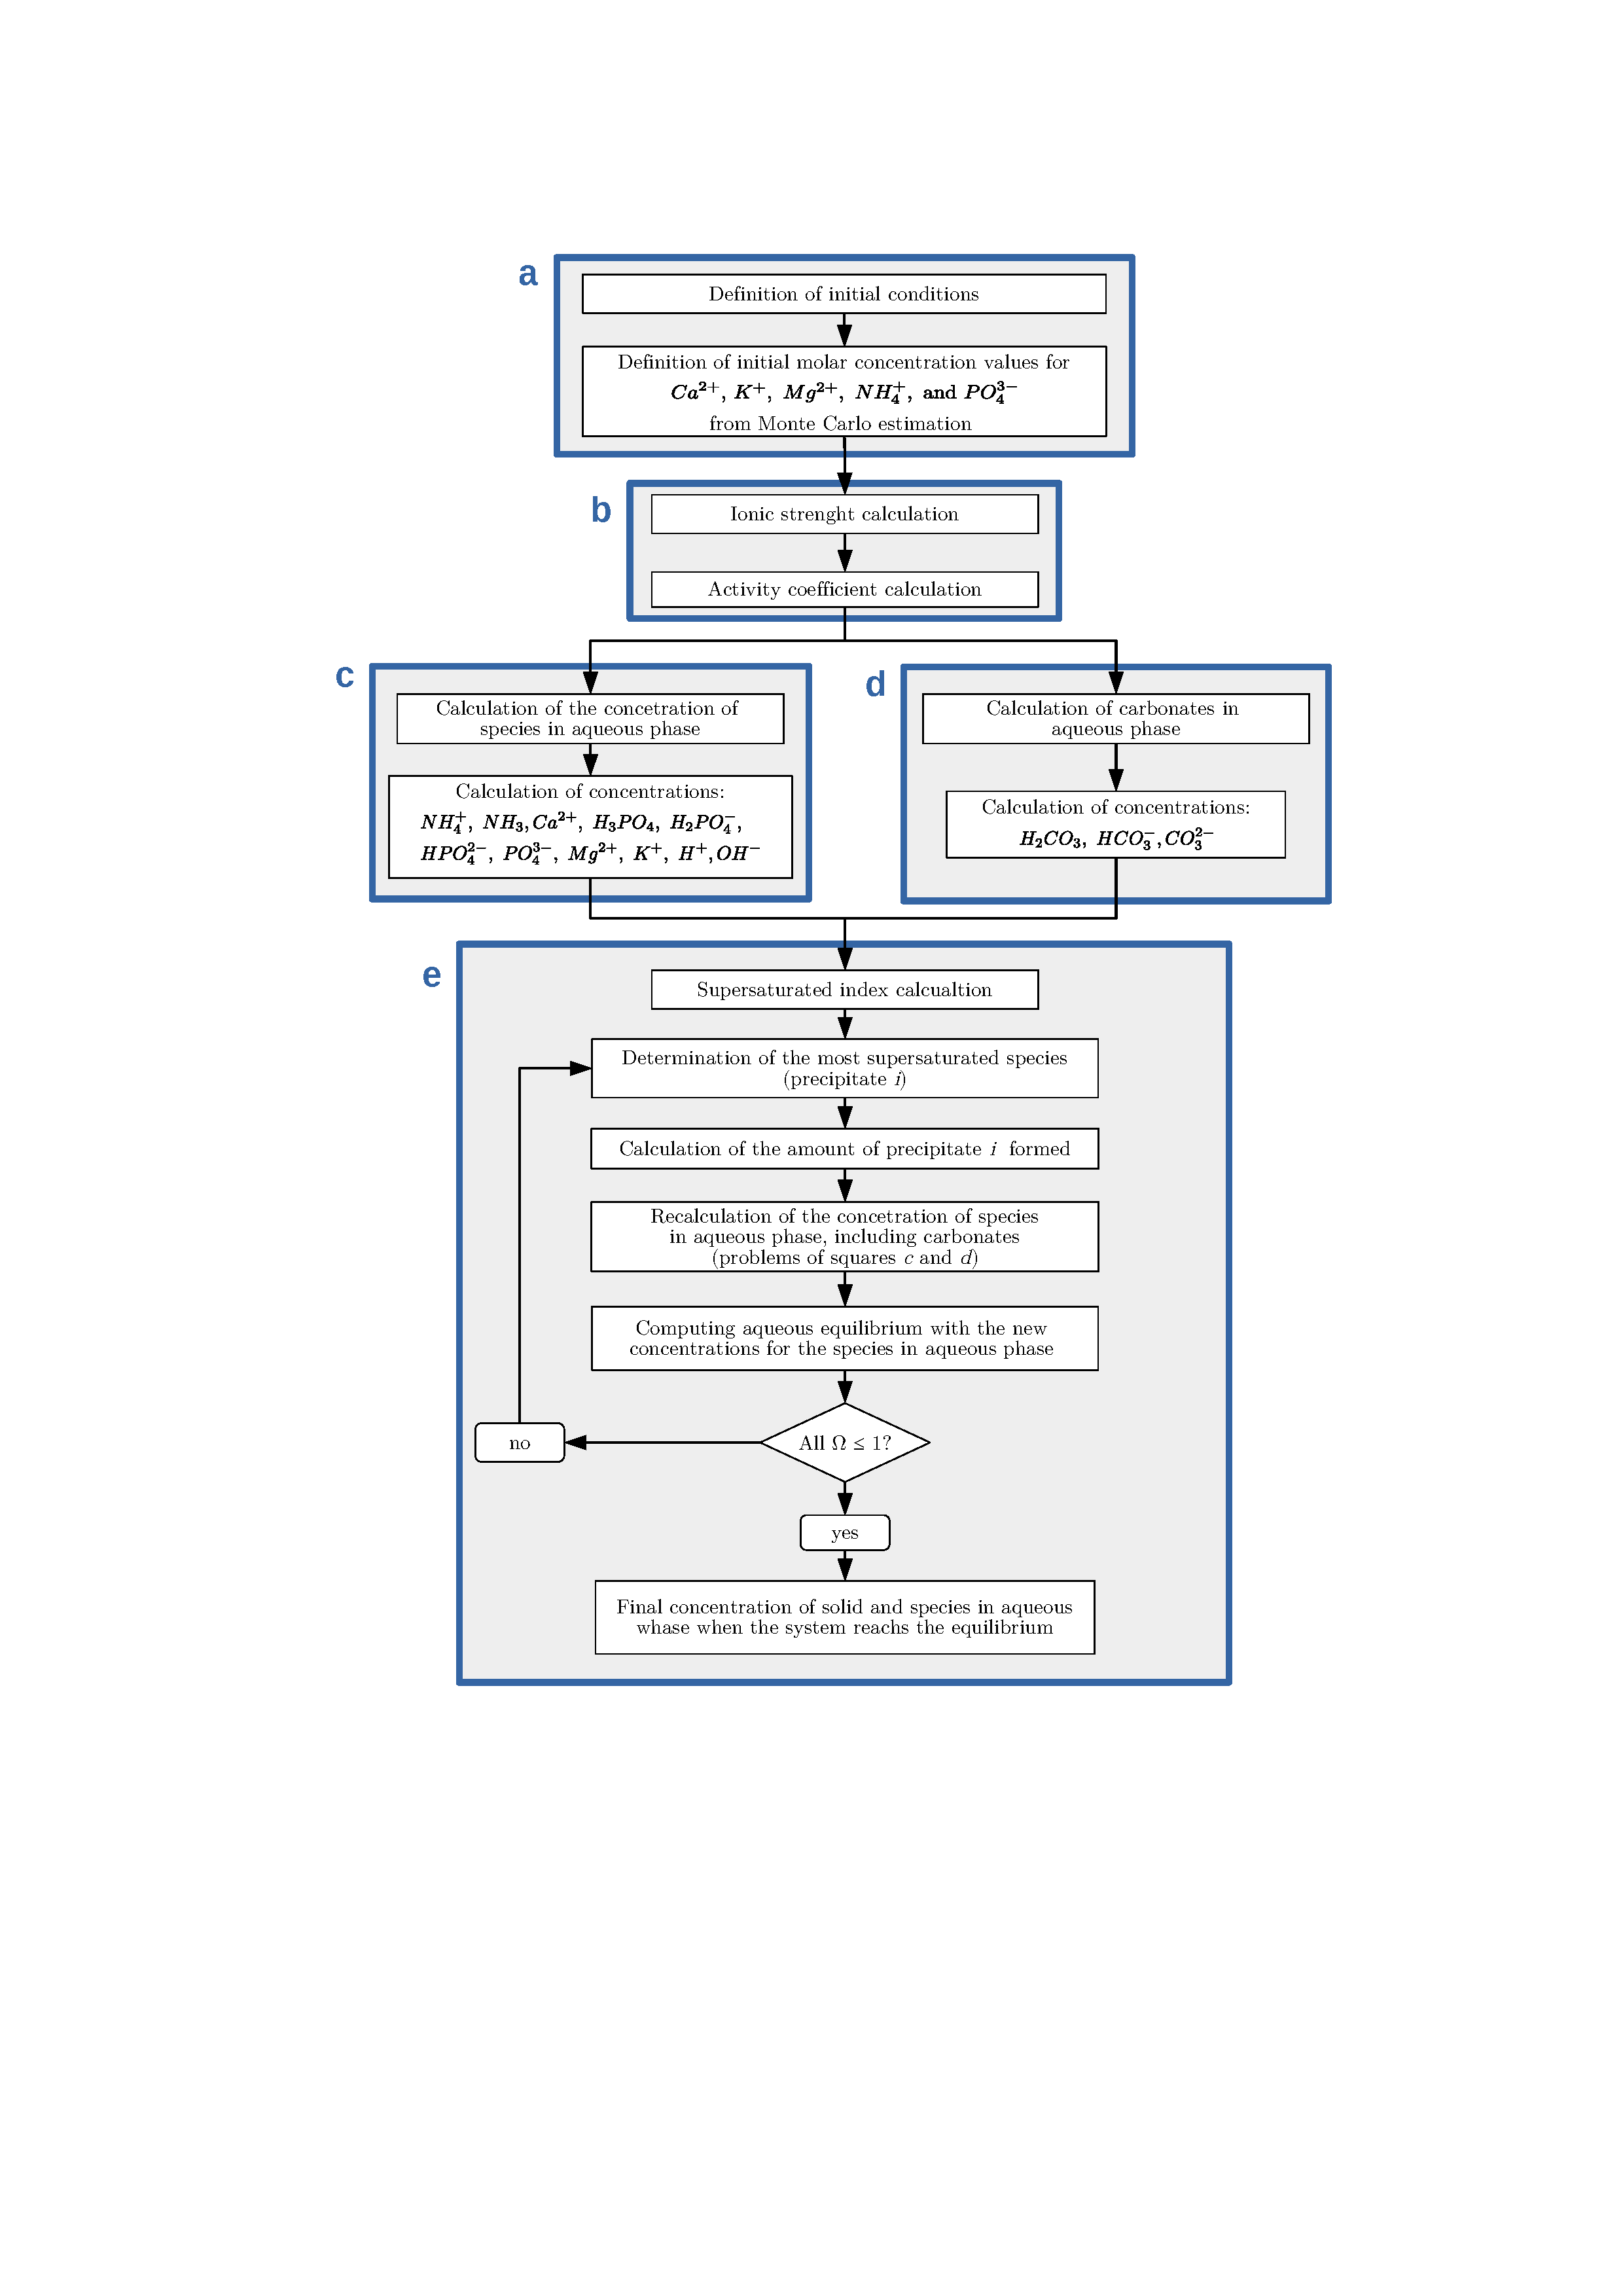
\includegraphics[width=\textwidth, trim=6cm 15cm 6cm 6cm, clip]{gfx/Chapter3/algorithm_flowsheet_w_squares_SUPERREDUCED.pdf} 
	\caption{Flowchart of the proposed algorithm to solve the thermodynamic model for the formation of precipitates in cattle organic waste.} \label{fig:alg_flow}
\end{figure}

\subsubsection{Integration of waste composition uncertainty and precipitates formation thermodynamic models}
\begin{figure}[h]
	\begin{adjustwidth}{}{} 
		\centering
		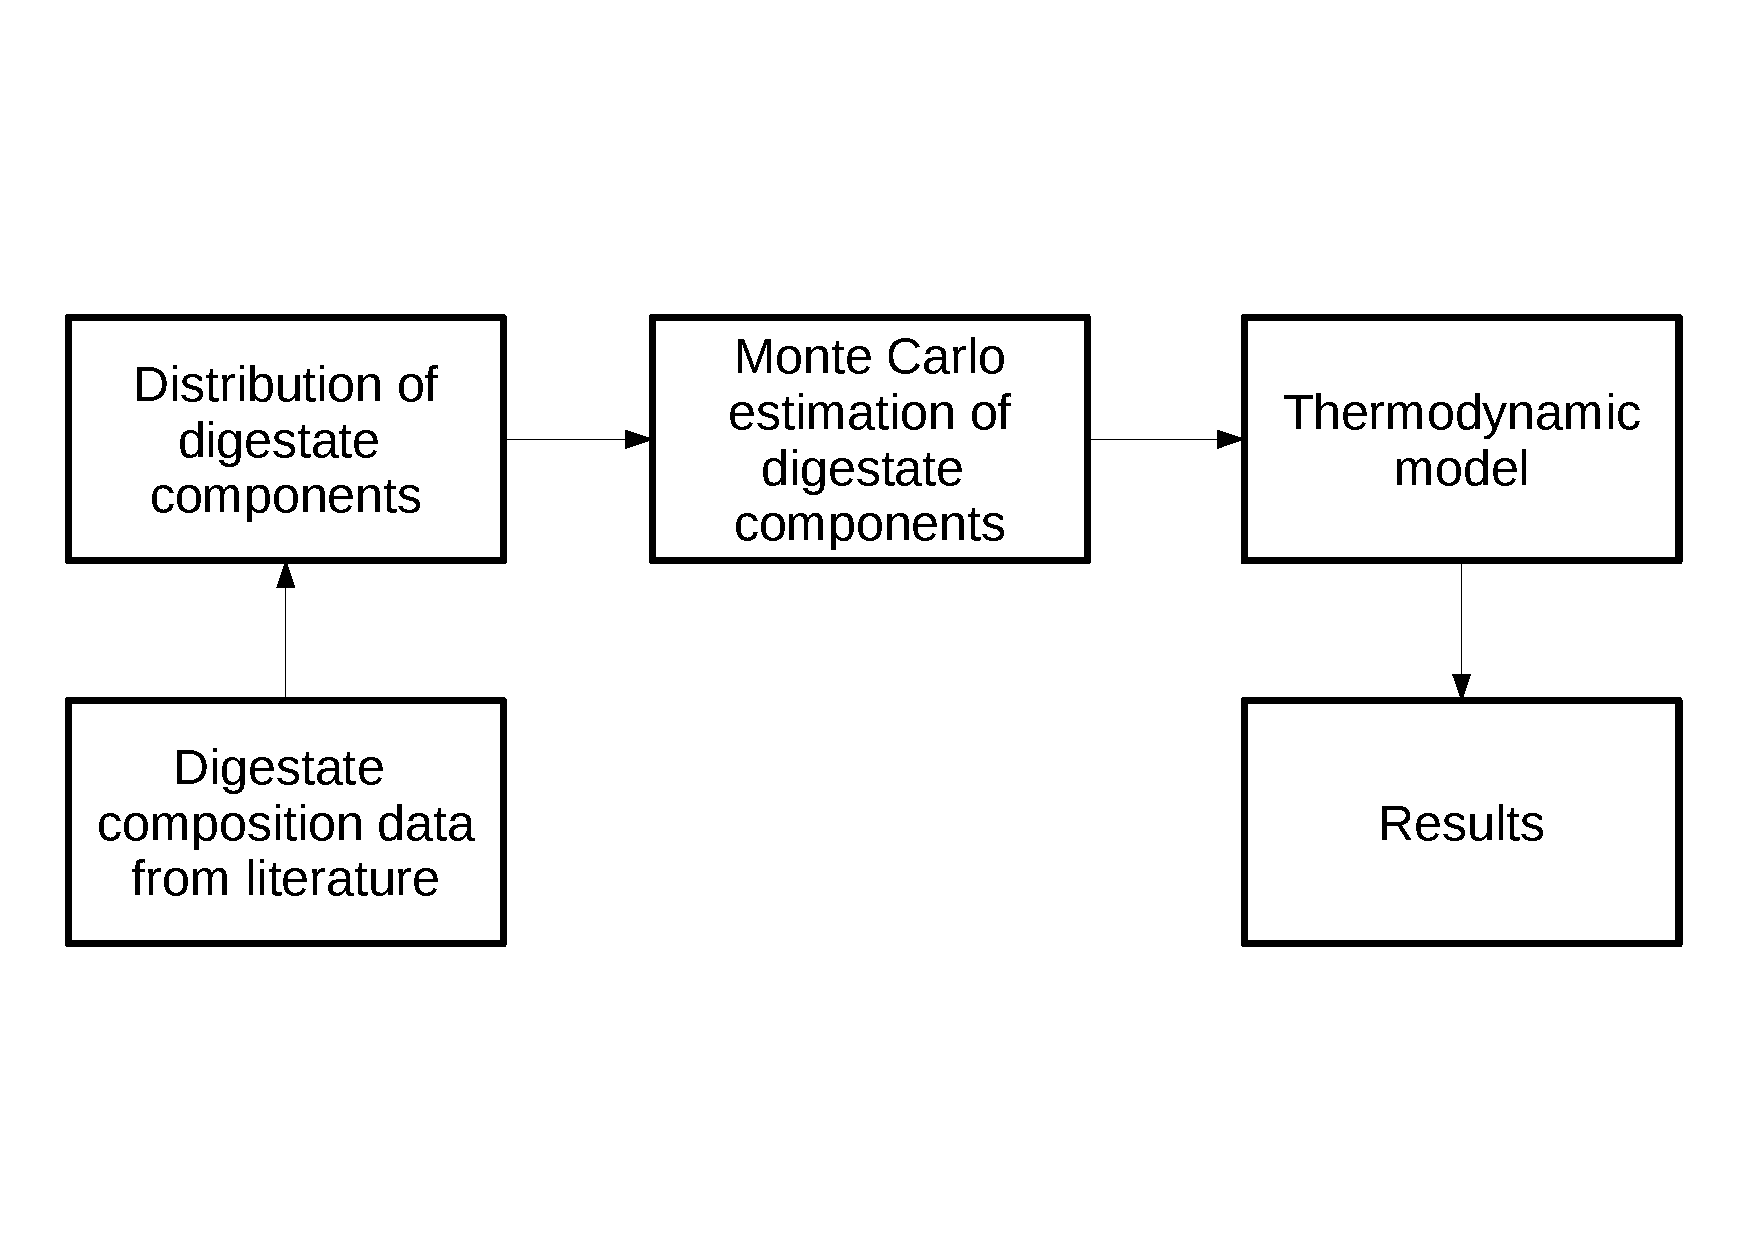
\includegraphics[width=0.7\textwidth, trim=0 4.5cm 0 5cm, clip]{gfx/Chapter3/procedure} 
		\caption{A solution procedure to evaluate the influence of the cattle waste composition variability in the formation of struvite.} \label{fig:procedure_schema}
	\end{adjustwidth}{}
\end{figure}
The evaluation of livestock waste variability in the formation of struvite and other precipitates, consists of 5 steps, as shown in Fig. \ref{fig:procedure_schema}. First, cattle waste composition data are collected from literature. Using these data, probability density distributions for the compounds of cattle leachate are estimated, and they are used in the Monte Carlo model to obtain feasible composition data sets of cattle organic waste. Random points are generated for each chemical compound and species ratios (i.e. N, P, K, Ca, $\text{N-NH}_{4}^{+}:\text{N}_\text{total}$, and $\text{P-PO}_{4}^{3-}:\text{P}_{\text{total}}$). 
Finally, the thermodynamic model is solved for the composition data sets generated, obtaining the precipitated compounds formed.

The thermodynamic model has been implemented in the algebraic modeling language JuMP, embedded in the programming language Julia \citep{DunningHuchetteLubin2017, bezanson2017julia}. The statistical study of cattle waste composition data, the Monte Carlo framework, result analysis, and data visualization were made in Python language \citep{Python, Numpy, Matplotlib, Pandas}.

\subsubsection{Model validation and limitations}
The developed model was validated using the data provided by \citet{Zeng}. Their work was carried out under similar operational conditions to which this work intends to evaluate. In Fig. \ref{fig:validation} experimental and model results are compared. The values at high $\text{Mg}^{2+}$ molar ratio, when the largest supersaturation values are reached and the formation of struvite is close to the maximum allowed by the thermodynamic equilibrium, match the experimental data. However, at lower ratios, differences between results of the thermodynamic model proposed and experimental data can be observed. As the authors of the article indicate, this differences can be due to the presence of many suspended solids which interfere in the struvite formation process. Note that this work is focused on the thermodynamic aspect, without considering other aspects such as chemical kinetics or transport phenomena. The scarcity of data is an impediment to further validate the model.
\begin{figure}[h] 
	\centering
	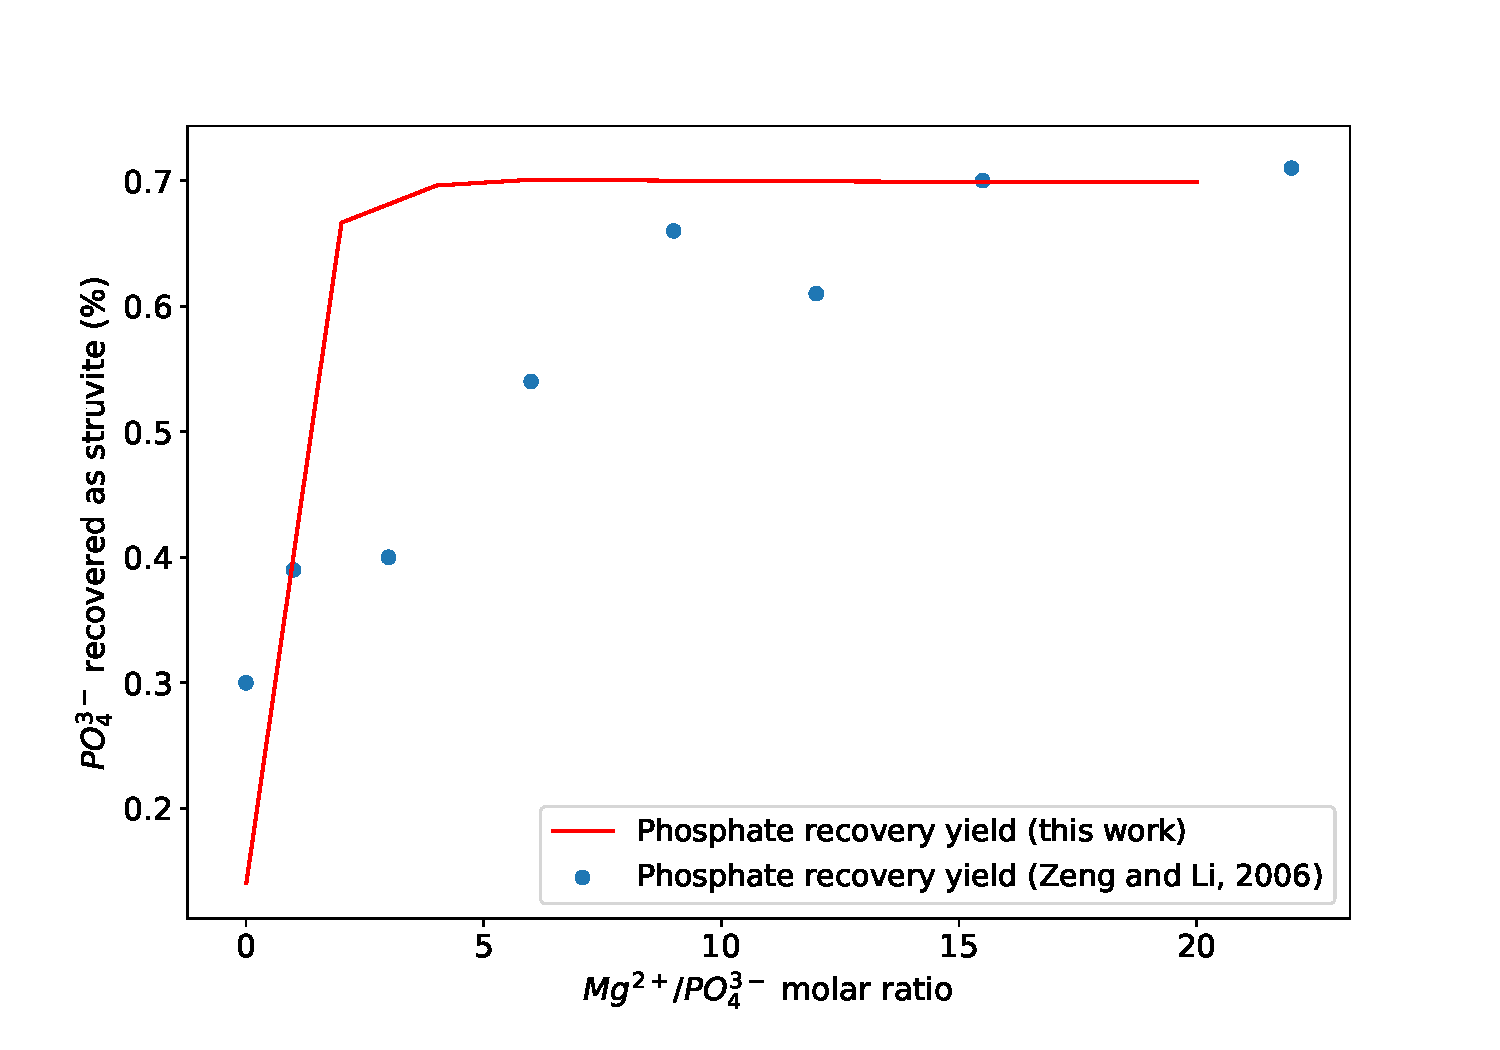
\includegraphics[width=0.9\textwidth, trim=0 0cm 0 1.5cm, clip]{gfx/Chapter3/validation.pdf} 
	\caption{Comparison between experimental results reported by \protect\citet{Zeng} and the results provided by the model developed in this work.} \label{fig:validation}
\end{figure}

In addition to the lack of previous studies and data availability to evaluate the effects of kinetics and transport phenomena in the formation precipitates from cattle leachate, another improvement of the proposed model can be achieved by the experimental determination of pKsp values for the potential precipitates formed from cattle leachate. For struvite, the selected pKsp value is taken from the work of \citet{Ohlinger}, as they determined the pKsp value for struvite formation in digestate, a medium with high organic load and dissolved elements like cattle leachate. Otherwise, when pKsp data for cattle waste is unavailable from previous studies, the reported values for water are used. A limitation in the use of the obtained surrogate models is that the formation of struvite and calcium precipitates can only be determined for cattle waste. Although a general formulation for the thermodynamic model is used, and the methodology proposed to include the effect of the uncertainty is not restricted to the use of a specific waste, only cattle leachate has been considered in this study. However, if data on the composition is available, surrogate models to predict the formation of struvite and calcium precipitates from other waste sources can be easily developed.

\section{Results and discussion}
\subsection{Surrogate models to estimate the formation of precipitates from livestock organic waste} \label{results}
The influence of the main controllable parameters for struvite production at industrial scale operation was evaluated: the presence of magnesium and calcium, and the alkalinity. Surrogate models were developed to allow the analytical estimation of precipitates formation. pH value for the struvite precipitation process has been considered as a fixed variable, since there is a wide consensus about a pH value of 9, at which struvite solubility is minimum, is optimal, enhancing the phosphorus and nitrogen conversion to struvite and its eventual precipitation \citep{Tao, Zeng}.

\subsubsection{Influence of magnesium} \label{inf_Mg}
In phosphorus recovery processes through struvite formation, magnesium is usually added to increase the saturation of struvite, enhancing its precipitation. This is especially important for cattle leachate due to the high presence of calcium ions competing with other cations for phosphate anions, and the high ionic strength of livestock leachate, reducing the effective concentration of ions. If the supplementation of magnesium provides enough magnesium ions, struvite will reach higher supersaturation ratio than calcium precipitates, leading the formation of struvite over calcium compounds.
To estimate the performance of struvite precipitation from cattle leachate, the developed thermodynamic model was solved for 50 different composition data sets. The average alkalinity value of the range reported by \citet{Tao} is considered, 8770.5 mg of $\text{CaCO}_{3}$.
The plots showing evolution of precipitates formation in function of the  $\text{Mg}^{2+}/\text{PO}_{4}^{3-}$ molar ratio are collected in the Supplementary Material. 
Analyzing the average fraction of $\text{PO}_{4}$ recovered in form of struvite as a function of the $\text{Mg}^{2+}/\text{PO}_{4}^{3-}$ molar ratio, a tentative value for $\text{Mg}^{2+}/\text{PO}_{4}^{3-}$ molar ratio between 2 and 4 can be set as a compromise effectiveness-cost solution. Higher values result in a considerable consumption of magnesium returning lower improvements in phosphate recovery as struvite.
The surrogate model obtained to evaluate performance of struvite precipitation in function of the magnesium supplied is a Monod type equation, as shown in Eq. \ref{eq:monod_Mg_StrYield}, where $x_{\text{Mg}^{2+}:\text{PO}_{4}^{3-}}$ is referred to the $\text{Mg}^{2+}/\text{PO}_{4}^{3-} \ \text{molar ratio}$.

\begin{align}
& x_{\text{struvite} \left(\text{PO}_{4}^{3-}\right)} = \frac{0.957 \cdot x_{\text{Mg}^{2+}:\text{PO}_{4}^{3-}}}{0.996 + x_{\text{Mg}^{2+}:\text{PO}_{4}^{3-}}} \label{eq:monod_Mg_StrYield} 
\end{align}

The evolution in the formation of calcium precipitates as a function of the $\text{Mg}^{2+}/\text{PO}_{4}^{3-}$ molar ratio was also studied. Hydroxyapatite and calcium carbonate are the only calcium precipitates produced.
Both hydroxyapatite and $\text{CaCO}_{3}$ patterns can be related to the increment of struvite formation along the increase of $\text{Mg}^{2+}/\text{PO}_{4}^{3-}$ molar ratio values, which reduces the presence of phosphate ions, and consequently decreases the supersaturation of hydroxyapatite. Therefore, there are more calcium ions available to form calcium carbonate. 
Surrogate models fit to first order polynomial equations for hydroxyapatite, Eq. \ref{eq:1poly_Mg_HAP}, and for calcium carbonate, Eq. \ref{eq:1poly_Mg_CaCO3}.

\begin{align}
& x_{\text{hydroxyapatite} \left(\text{Ca}^{2+}\right)} = -1.299 \cdot 10^{-2} \cdot x_{\text{Mg}:\text{PO}_{4}^{3-}} + 0.248 \label{eq:1poly_Mg_CaCO3}\\
& x_{\text{CaCO}_{3} \left(\text{Ca}^{2+}\right)} = 1.296 \cdot 10^{-2} \cdot x_{\text{Mg}:\text{PO}_{4}^{3-}} + 0.749 \label{eq:1poly_Mg_HAP} 
\end{align}

\subsubsection{Influence of calcium}
One of the hindrances of cattle leachate for struvite precipitation is the presence of calcium ions competing with other cations for phosphate to form different precipitates.
To study the inhibitory influence of calcium in cattle leachate for struvite precipitation, the thermodynamic model was evaluated for the same 50 different composition data sets used in the previous study along $\text{Ca}^{2+}/\text{PO}_{4}^{3-}$ molar ratio values from 0 to 5. To exclude the influence of magnesium concentration, the study was carried out fixing the $\text{Mg}^{2+}/\text{PO}_{4}^{3-}$ molar ratio at 2.
The plots showing evolution of precipitates formation in function of the $\text{Ca}^{2+}/\text{PO}_{4}^{3-}$ molar ratio are collected in the Supplementary Material. 

The phosphorus as phosphate fraction recovered as struvite exhibits a steep descent at $\text{Ca}^{2+}/\text{PO}_{4}^{3-}$ values between 0 and 2, followed by an asymptotic behavior tending to 0. The dispersion of the values has slight variations along with the evaluated $\text{Mg}^{2+}/\text{PO}_{4}^{3-}$ values.
For hydroxyapatite and calcium carbonate, the higher $\text{Ca}^{2+}/\text{PO}_{4}^{3-}$ value, the greater dispersion for the obtained values. This is due to the increase in the supersaturation values for both calcium precipitates because of the presence of a higher number of calcium ions in the leachate.

The surrogate models obtained for struvite and calcium carbonate fit pseudo-sigmoidal equations, Eqs. \ref{eq:sigmoidal_Ca_StrYield} and \ref{eq:sigmoidal_CaCaCO3} respectively; while for hydroxyapatite (HAP) is a second polynomial function, Eq. \ref{eq:sigmoidal_Ca_HAP}. In all cases, $ x_{\text{Ca}^{2+}:\text{PO}_{4}^{3-}}$ is referred to $\text{Ca}^{2+}/\text{PO}_{4}^{3-} \ \text{molar ratio}$.

\begin{align}
&x_{\text{struvite} \left(\text{PO}_{4}^{3-}\right) }= \frac{0.798}{1+\left(x_{\text{Ca}^{2+}:\text{PO}_{4}^{3-}} \cdot 0.576\right)^{2.113}} \label{eq:sigmoidal_Ca_StrYield} \\
\nonumber \\
\begin{split}
& x_{\text{hydroxyapatite} \left(\text{Ca}^{2+}\right)} = -4.321 \cdot 10^{-2} \cdot x_{\text{Ca}^{2+}:\text{PO}_{4}^{3-}}^{2} + 0.313 \cdot x_{\text{Ca}^{2+}:\text{PO}_{4}^{3-}} \\& \hspace{7.8cm} - 3.619 \cdot 10^{-2} \label{eq:sigmoidal_Ca_HAP}
\end{split}
\\
\nonumber \\
&  x_{\text{CaCO}_{3} \left(\text{Ca}^{2+}\right)} = \frac{1.020}{1+\left(x_{\text{Ca}^{2+}:\text{PO}_{4}^{3-}} \cdot 0.410 \right)^{1.029}} \label{eq:sigmoidal_CaCaCO3}
\end{align}

\subsubsection{Influence of alkalinity}
Alkalinity is a parameter which can be used to control the production of calcium precipitates. When the presence of carbonates is low, the competition between hydroxyapatite and calcium carbonate tends to benefit the first compound because the limited availability of carbonate ions reduces the supersaturation of calcium carbonate. However, the predominance of hydroxyapatite reduces the formation of struvite since both elements compete for phosphate ions. Therefore, the presence of significant amounts of carbonates (performing at alkaline conditions) reduces the formation of hydroxyapatite and promotes the formation of struvite. 

The results for the formation of struvite, hydroxyapatite and calcium carbonate considering the same 50 different composition data sets used in the previous studies  in function of the alkalinity are collected in the Supplementary Material.
It can be observed that the behavior of struvite formation and calcium carbonate are related, with an abrupt change for both elements at alkalinity values between 3,000 and 4,000 mg of $\text{CaCO}_{3}$, reaching plateaus beyond these values. The dispersion of values follow a similar pattern for both struvite and calcium carbonate, being lower at low alkalinity values, and progressively growing until reaching a value of 4,000 mg of $\text{CaCO}_{3}$. Beyond this value, the dispersion of  values remains constant. Hydroxyapatite formation decrease continuously along the alkalinity values, being complementary with the formation of calcium carbonate.

Therefore, struvite formation from livestock leachate can be enhanced inhibiting hydroxyapatite formation by controlling the alkalinity level, increasing the formation of calcium carbonate and reducing the concentration of calcium ions competing for phosphate. 
Pseudo-sigmoidal fits are shown in Eq. \ref{eq:sigmoidal_Alk_StrYield} for $x_{struvite \left(PO_{4}^{3-}\right)}$, Eq. \ref{eq:sigmoidal_Alk_HAP} for the case of hydroxyapatite, and Eq. \ref{eq:sigmoidal_Alk_CaCO3} for calcium carbonate, where $ x_{Alk}$ is referred to $\text{alkalinity} \left( \text{mg } |\text{CaCO}_{3}\right)$.

\begin{align}
& x_{\text{struvite} \left(\text{PO}_{4}^{3-}\right)} = \frac{0.695}{1+\left(x_{\text{Alk}} \cdot 4.229 \cdot 10^{-4}\right)^{-2.638}} \label{eq:sigmoidal_Alk_StrYield} \\
\nonumber \\
& x_{\text{hydroxyapatite} \left(\text{Ca}^{2+}\right)} = \frac{0.260}{1+\left(x_{\text{Alk}} \cdot 6.460 \cdot 10^{-5}\right)^{3.390}} \label{eq:sigmoidal_Alk_HAP} \\
\nonumber \\
& x_{\text{CaCO}_{3} \left(\text{Ca}^{2+}\right)} = \frac{0.847}{1+\left(x_{\text{Alk}} \cdot 4.646 \cdot 10^{-4}\right)^{-1.870}} \label{eq:sigmoidal_Alk_CaCO3}
\end{align}

\subsubsection{Interactions between calcium and magnesium to phosphate ratios}
Interactions between calcium and magnesium to phosphate ratios were evaluated to determine a target operational area for optimal struvite production performance. In Fig. \ref{fig:struvite_precipitation} the formation of struvite as function of $\text{Mg}^{2+}/\text{PO}_{4}^{3-}$ and $\text{Ca}^{2+}/\text{PO}_{4}^{3-}$ molar ratios is shown, where the area with the highest phosphate recovery in form of struvite has been shaded. It can be observed that struvite formation depends strongly on the $\text{Ca}^{2+}/\text{PO}_{4}^{3-}$ molar ratio. For $\text{Ca}^{2+}/\text{PO}_{4}^{3-}$ values less than 3 struvite formation reaches the maximum values, even for low $\text{Mg}^{2+}/\text{PO}_{4}^{3-}$ molar ratio values. For high calcium/phosphate ratios, struvite formation decreases abruptly, obtaining low increases in struvite formation  even for large supplies of magnesium.

\begin{figure}[h] 
	\begin{adjustwidth}{}{}
		\centering
		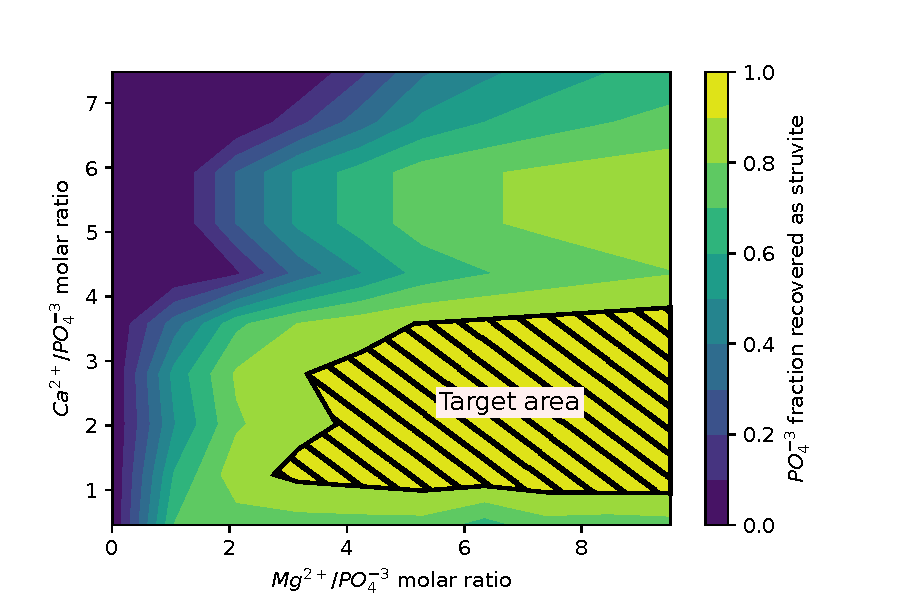
\includegraphics[width=0.6\linewidth, trim=0.5cm 0cm 1cm 1cm, clip]{gfx/Chapter3/Contour_plot_mod.pdf} 
		\caption{Influence of magnesium and calcium in struvite precipitation.} 
		\label{fig:struvite_precipitation}
	\end{adjustwidth}{}
\end{figure}

\subsection{Phosphorus releases from cattle leachate potentially avoided via struvite formation}
Phosphorus pollution of waterbodies, followed by eutrophication and hypoxia scenarios, represents a major environmental problem for the current societies. Considering the United States, the Census of Agriculture reports more than 93 million of cattle heads \citep{2017CensusofAgriculture}, generating an estimated amount of 1,144 million of tons of organic waste per year. The phosphorus contained in the organic waste can be lost as runoff, reaching waterbodies, and polluting the surrounding aquatic ecosystems. Actually, several outstanding cases of eutrophication have taken place in the U.S. in recent times, such as the events occurred in Lake Erie since 1990, and the dead zone in the Gulf of Mexico because of in-excess nutrients discharges collected along the Mississippi River basin. Therefore, nutrient recovery strategies must be implemented to capture phosphorus (and nitrogen) before reaching the waterbodies. Additionally, phosphorus recovery as struvite allows its redistribution to nutrient deficient areas \citep{Martin}.
The surrogate models developed are used to estimate the potential phosphorus emissions avoided in each watershed through phosphorus recovery from cattle leachate as struvite. 

\subsubsection{Balance of phosphorus involved in agricultural activities throughout the U.S. watersheds}
To reach environmental sustainability and reduce the impact over the original ecosystems as much as possible, the releases of phosphorus should be balanced with a coordinated network of phosphorus uptakes. To determine the balance between the releases and uptakes of phosphorus from the agricultural sector, the TES sustainability metric is computed for each watershed in the U.S., showing the watersheds where the phosphorus releases are unbalanced and impacting the environment, Fig. \ref{fig:TES}. For a total of 2,104 HUC8 watersheds, data is unavailable for 6 watersheds, the phosphorus releases and uptakes are balanced in 1,410 watersheds, and 691 exhibit unbalanced phosphorus releases, representing the 33.12\% of total watersheds. It can be observed a larger concentration of unbalanced watersheds along the Mississippi River basin and around the Lake Erie, areas currently affected by eutrophication issues. 

For studies requiring higher spatial resolution, more accurate values for the TES metric can be stimated through the use of local inventories for phosphorus releases and uptakes. A dataset with the phosphorus releases and uptakes, the phosphorus balance, and the TES metric computed for each watershed are available in the Supplementary Material. A dataset with the phosphorus releases and uptakes, the phosphorus balance, and the TES metric computed for each watershed are available in the Supplementary Material.

\begin{figure}[h] 
	\begin{adjustwidth}{}{}
		\centering
		\includegraphics[width=\linewidth]{gfx/Chapter3/TES_mod.png} 
		\caption{Techno-ecological synergy (TES) metric values for HUC8 watersheds. Red indicates watersheds with unbalanced agricultural phosphorus releases, and blue indicates watersheds with balanced agricultural phosphorus releases. White indicates watersheds with not available data.} 
		\label{fig:TES}
	\end{adjustwidth}{}
\end{figure}

\subsubsection{Phosphorus recovered from cattle leachate through struvite precipitation}
\begin{sidewaysfigure}
	\begin{subfigure}[t]{0.49\textheight}
		\includegraphics[width=\textwidth, trim=55cm 30cm 0cm 0cm, clip]{gfx/Chapter3/scenario1.png}
		\caption{Scenario 1}
		\label{fig:scenario1}
	\end{subfigure}
	%	\quad
	\begin{subfigure}[t]{0.49\textheight}
		\includegraphics[width=\textwidth, trim=55cm 30cm 0cm 0cm, clip]{gfx/Chapter3/scenario2.png} 
		\caption{Scenario 2}
		\label{fig:scenario2}
	\end{subfigure}
	\\
	\begin{subfigure}[t]{0.49\textheight}
		\includegraphics[width=\textwidth, trim=55cm 30cm 0cm 0cm, clip]{gfx/Chapter3/scenario3.png}
		\caption{Scenario 3}
		\label{fig:scenario3}
	\end{subfigure}
	%	\quad
	\begin{subfigure}[t]{0.49\textheight}
		\includegraphics[width=\textwidth, trim=55cm 30cm 0cm 0cm, clip]{gfx/Chapter3/scenario4.png}
		\caption{Scenario 4}
		\label{fig:scenario4}
	\end{subfigure}
	
	\caption{Phosphorus releases avoided through struvite production for the different scenarios considered. Darker colors represent larger phosphorus recovery}
	\label{fig:plot_scenarios}
\end{sidewaysfigure}

Since the scope of the surrogate models developed is limited to the treatment of cattle leachate, only P releases from cattle organic waste will be considered for recovery. Additionally, as it is mentioned in the description of the model, only the phosphate fraction of phosphorus can be recovered through struvite precipitation. Data provided by IPNI NuGIS \citep{NuGIS} report total manure generated, but do not report the breakdown of manure generated by different livestock sources. Therefore, the inventory of cattle for each HUC6 watershed reported by the U.S. Census of Agriculture is used \citep{2017CensusofAgriculture}. To keep spatial consistency between data, the inventory of cattle was aggregated from HUC6 to HUC8 watershed level scaling by the fraction of area represented by each HUC8 basin over the total HUC6 area. The breakdown of cattle types in the U.S. Census of Agriculture is not available at watershed level, but it is available at state level. Therefore, the number of cattle heads is weighted by the fraction of milk and beef animals in the corresponding state. finally, the animals number for each type of cattle is calculated using the normalization values provided by Kellog et al. (2010) \citep{Kellog2000}. If the watershed is shared among several states, the average of the represented states is considered.

Since the supply of magnesium is the easiest controllable variable in the struvite precipitation process, the scenarios evaluated to determine the phosphorus emissions avoided through struvite precipitation were defined through the use of different amounts of magnesium using the surrogate model shown in Eq. \ref{eq:monod_Mg_StrYield}. The different supplies of magnesium have a direct influence on the economy of the process, being one of the highest operating costs items. A summary of the scenarios evaluated and the results obtained is presented in Table \ref{table:scenarios}. The fraction of phosphorus releases avoided is computed over the total phosphorus releases from agricultural activities, including manure releases and fertilizer application, as described in Section \ref{Preleases}. 

\begin{table}[h]
	\centering
	\caption{Scenarios considered and results for cattle leachate phosphorus recovery} \label{table:scenarios}
	\resizebox{\columnwidth}{!}{
	\begin{tabular}{@{}ccccc@{}}
		\toprule
		Scenario                                                                                           & 1       & 2       & 3       & 4       \\ \midrule
		\begin{tabular}[c]{@{}c@{}}$\text{Mg}^{2+}/\text{PO}_{4}^{3-}$ \\ molar ratio\end{tabular}                             & 1       & 2       & 4       & 6       \\
		\begin{tabular}[c]{@{}c@{}}Total P releases avoided\\ (total watersheds) (tons)\end{tabular}       & 422,104 & 562,430 & 674,556 & 722,573 \\
		\begin{tabular}[c]{@{}c@{}}Average P releases avoided\\  (total watersheds) (\%)\end{tabular}      & 22.63   & 30.16   & 36.17   & 38.75   \\
		\begin{tabular}[c]{@{}c@{}}Average P releases avoided\\  (unbalanced watersheds) (\%)\end{tabular} & 18.07   & 24.08   & 28.88   & 30.94   \\
		$\text{kg Mg} / \text{kg P}_{\text{recovered}}$  
		& 2.68    & 4.02    & 6.71    & 9.40    \\ \bottomrule
	\end{tabular}
	}
\end{table}

The results for each scenario considered at watershed scale are shown in Fig. \ref{fig:plot_scenarios}, where darker colors represent larger phosphorus releases avoided. It can be observed that struvite production can contribute to reducing phosphorus emissions around Lake Erie and the Great Lakes region, one of the most severely affected areas by eutrophication problems. Additionally, other areas where the phosphorus emissions avoided are especially significant are the upper basin of the Mississippi River, and the basins located in the south-central region of the United States, such as the areas of some tributaries rivers to the Mississippi River basin, the Rio Grande river and the Colorado River basin. At national level, struvite production can contribute to reduce the agricultural phosphorus releases by 22\% for most conservative case where the lowest amount of magnesium is added. The phosphorus fraction recovered raises until a 30\% and 36\% when the amount of magnesium added is multiplied by 2 and by 4 respectively. However, for the scenario 4 the increase in the supply of magnesium only increases the phosphorus recovered in 2 percentual points compared with the previous scenario. Therefore, the implementation of struvite production processes for phosphorus recovering in cattle facilities can contribute significantly to the reduction in the phosphorus emissions from agricultural operations, reducing the runoffs to waterbodies and mitigating the nutrient pollution of the aquatic ecosystems. However, when only unbalance watersheds are  considered, the average fraction of phosphorus releases avoided decreases, suggesting that, from a global overview, the phosphorus releases due to fertilizers play a major role in these watersheds than when balance and unbalance watersheds are evaluated altogether. Data at watershed level are collected in the Supplementary Material.

Therefore, the phosphorus recovered from livestock facilities have a significant impact in the reduction of phosphorus releases to the environment. However, to achieve a successful implementation of nutrient management strategies, coordinated network management efforts to mitigate nutrient pollution of aquatic systems including point and non-point sources, should be performed for optimizing nutrient management programs that minimize the capital and operating costs while maximizing the environmental benefits. Proposals for the development of coordinated management systems for organic wastes have been presented by \citet{Sharara}, \citet{Sampat3}, and \citet{hu_logistics_2019}.

\section{Conclusions}
To estimate the potential phosphorus releases avoided through struvite precipitation from cattle waste, a thermodynamic framework has been developed to evaluate struvite production from cattle organic waste as a technology for nutrient management and recovery. A set of practical numerical correlations is developed to help predict the struvite recovery. Cattle waste treatment and nutrient recovery through struvite formation is a feasible process from a thermodynamic perspective, reaching phosphate recovery efficiencies up to 80\% with the addition of considerable amounts of magnesium. Additionally, the results show that alkaline conditions can control the calcium ions when their presence in the medium is high and these can interfere in the formation of struvite by precipitating the calcium ions as calcium carbonate, and enhancing the recovery of phosphate as struvite. However, the variability in the organic waste composition is an important parameter that has a high impact on the efficiency of the process. Therefore, an individual composition analysis of the treated cattle waste should be the ideal procedure to achieve the optimal performance of the process by adjusting the operating conditions, particularly the amount of magnesium added and the alkalinity of the medium. Nevertheless, there are opportunities for improving the proposed model by the experimental determination of pKsp values for all potential precipitates from cattle leachate, and by including the effects from kinetics and transport phenomena. 

The techno-ecological synergy sustainability metric (TES) is a useful tool for visualizing the spatial distribution of environmental problems, making it possible to determine what areas are  more sensible to nutrient pollution, and allowing an adequate distribution of efforts to mitigate phosphorus releases and achieved better nutrient management practices. In the U.S., struvite production has large potential for reducing the phosphorus losses from livestock facilities, avoiding between the 22\% and the 36\% of the phosphorus releases from the agricultural sector at national level, reducing the phosphorus runoff and mitigating the nutrient pollution of waterbodies. In addition, it can be observed how struvite production can significantly contribute to reducing phosphorus emissions around Lake Erie and the Great Lakes region, some of the most severely affected areas by eutrophication problems. It should be remarked that the production of struvite from cattle leachate allows the redistribution of phosphorus to nutrient deficient areas reducing the phosphorus runoff to waterbodies and mitigating the nutrient pollution of aquatic ecosystems. However, future research is needed to consider temporal aspects, transportation logistics, and coordinated management strategies for achieving global solutions to global problems. 

\section*{Acknowledgments} \label{section:Ch3Acknowledgments}
\addcontentsline{toc}{section}{Acknowledgments}
We acknowledge funding from the Junta de Castilla y Le\'{o}n, Spain, under grant SA026G18 and grant EDU/556/2019, and by an appointment for E. Mart\'{i}n-Hern\'{a}ndez to the Research Participation Program for the Office of Research and Development, U.S. EPA, administered by the Oak Ridge Institute for Science and Education. 

\textbf{Disclaimer:} The views expressed in this article are those of the authors and do not necessarily reflect the views or policies of the U.S. EPA. Mention of trade names, products, or services does not convey, and should not be interpreted as conveying, official U.S. EPA approval, endorsement, or recommendation.

\section*{Bibliography}
\addcontentsline{toc}{section}{Bibliography}

\printbibliography[heading=none]
\end{refsection}
%\cleardoublepage%*****************************************
\chapter{Geospatial environmental and techno-economic framework for	sustainable phosphorus management at livestock facilities}\label{ch:Tool}
%*****************************************
\section{Introduction}

%\cleardoublepage%*****************************************
\chapter{Analysis of incentive policies for phosphorus recovery}\label{ch:Policies}
%*****************************************
\begin{refsection}[referencesCh5]
\section*{Abstract}
Livestock operations have been highly intensified over the last decades, resulting in the advent of large concentrated animal feeding operations (CAFOs). Intensification decreases production costs but also leads to substantial environmental impacts. Specifically, nutrient runoff from livestock waste results in eutrophication, harmful algal blooms, and hypoxia. The implementation of nutrient recovery systems in CAFOs can abate nutrient releases and negative ecosystem responses, although they might negatively affect the economic performance of CAFOs. We design and analyze potential incentive policies for the deployment of phosphorus recovery technologies at CAFOs considering the geospatial vulnerability to nutrient pollution. The case study demonstration consists of 2,217 CAFOs in the U.S. Great Lakes area. The results reveal that phosphorus recovery is more economically viable in the largest CAFOs due to economies of scale, although they also represent the largest eutrophication threats. For small and medium-scale CAFOs, phosphorus credits progressively improve the profitability of nutrient management systems. The integration of biogas production does not improve the economic performance of phosphorus recovery systems at most of CAFOs, as they lack enough size to be cost-effective. Phosphorus recovery proves to be economically beneficial by comparing the net costs of nutrient management systems with the negative economic impact derived from phosphorus releases. The incentives necessary for avoiding up to $20.7 \cdot 10^3$ ton/year phosphorus releases and achieve economic neutrality in the Great Lakes area are estimated at \$223 million/year. Additionally, the fair distribution of limited incentives is studied using a Nash allocation scheme, determining the break-even point for allocating monetary resources.

\bigskip
Keywords: Organic waste; Incentive policy; Environmental policy; Livestock industry; Phosphorus recovery; Circular economy
\newpage

\section*{Resumen}
Las explotaciones ganaderas se han intensificado mucho en las últimas décadas, lo que ha dado lugar a la aparición de grandes explotaciones concentradas de alimentación animal (CAFO). La intensificación disminuye los costes de producción, pero también provoca importantes impactos ambientales. En concreto, la escorrentía de nutrientes procedente de los residuos ganaderos provoca eutrofización, floraciones de algas nocivas e hipoxia. La implantación de sistemas de recuperación de nutrientes en las CAFO puede reducir las emisiones de nutrientes y las respuestas negativas del ecosistema, aunque podría afectar negativamente a los resultados económicos de las CAFO. Diseñamos y analizamos posibles políticas de incentivos para la implantación de tecnologías de recuperación de fósforo en las CAFO teniendo en cuenta la vulnerabilidad geoespacial a la contaminación por nutrientes. El caso de demostración consiste en 2.217 CAFO en la zona de los Grandes Lagos de Estados Unidos. Los resultados revelan que la recuperación de fósforo es más viable económicamente en las CAFO más grandes debido a las economías de escala, aunque también representan las mayores amenazas de eutrofización. Para las CAFO de pequeña y mediana escala, los créditos de fósforo mejoran progresivamente la rentabilidad de los sistemas de gestión de nutrientes. La integración de la producción de biogás no mejora el rendimiento económico de los sistemas de recuperación de fósforo en la mayoría de las CAFO, ya que carecen del tamaño suficiente para ser rentables. La recuperación de fósforo demuestra ser económicamente beneficiosa al comparar los costes netos de los sistemas de gestión de nutrientes con el impacto económico negativo derivado de las emisiones de fósforo. Los incentivos necesarios para evitar hasta $20.7 \cdot 10^3$ toneladas/año de vertidos de fósforo y lograr la neutralidad económica en la zona de los Grandes Lagos se estiman en 223 millones de dólares/año. Además, se estudia la distribución justa de los limitados incentivos mediante un esquema de asignación de Nash, determinando el punto de equilibrio para la asignación de los recursos monetarios.

\bigskip
Palabras clave: Residuos orgánicos; Políticas de incentivos; Políticas ambientales; Industria ganadera; Recuperación de fósforo; Economía circular
\newpage


\section{Introduction}
In the context of continuous human population growth, an efficient and sustainable food production system becomes a key factor to guarantee social welfare. Currently, intensive livestock farming produces most of the meat and dairy products worldwide, and the demand is expected to double by 2050 compared to 2007 \citep{livestock_projection}. To meet this increasing demand, the development of intensive farming practices has resulted in the concentrated animal feeding operations (CAFOs) \citep{animal_unit_definition}, which allows larger and cheaper productivity than traditional systems. However, concerns in terms of food safety, animal health, and environmental impacts are associated with intensive livestock farming. Focusing on environmental impacts, livestock industry needs large amounts of water, represents 14.5\% of the anthropogenic-based GHG emissions \citep{eisler_agriculture:_2014}, and is a source of nutrient releases which lead to high concentrations of phosphorus in soil and waterbodies \citep{Sampat2017}. Focusing on nutrient pollution, phosphorus releases by improper organic waste management from livestock facilities contribute largely to the eutrophication of fresh and marine waters, promoting harmful algal blooms (HABs) which can release toxins and cause the hypoxia of waterbodies as a result of algae biomass decomposition. 

Therefore, the development of sustainable agricultural intensification techniques is not only a desirable but also a necessary measure to reduce the environmental impact of livestock industry while meeting the current and future food demand. In this regard, the implementation of integrated systems for manure management can recover valuable components contained in livestock waste, including phosphorus and biogas-based products, and the environmental footprint of CAFOs is decreased.

From a technical perspective, the adoption of nutrient management systems in CAFOs is feasible, but their practical implementation has to overcome several other logistical  and economic barriers.
Therefore, developing effective incentive policies to support the economic sustainability of livestock facilities plays a critical role in the successful adoption of phosphorus recovery technologies.
This is especially relevant because, despite the additional capital and operating costs these processes entail for the CAFOs, long-term remediation expense up to 74.5 USD per kg of released phosphorus \citep{Sampat2020} can be avoided by recovering phosphorus before it reaches soil and waterbodies. Remediation costs are believed to not affect the owners of livestock facilities directly; however, environmental remediation costs are usually covered by public budgets funded by taxpayers, and may lead to the eventual application of specific taxes on livestock products for their environmental footprint. Different incentive schemes can be considered to promote the adoption of sustainable nutrient management systems, including phosphorus releases allowances in the form of P credits and renewable electricity certificates (REC) for energy recovery.

In this work, a systematic analysis of different incentive schemes is performed through a computational framework for the techno-economic analysis of nutrient and energy recovery technologies for livestock facilities. Suitable nutrient and energy recovery technologies are determined for each studied CAFO among the state-of-the-art processes for organic waste management. The effect of different incentive policies on the economic performance of nutrient management technologies is studied considering the environmental vulnerability to nutrient pollution in the Great Lakes area. Additionally, the combination of incentives for the recovery of both phosphorus and electricity has been considered to identify potential synergies between the different technologies involved in the processing of livestock waste. The results obtained allow for the identification of the optimal incentive policies for the implementation of sustainable nutrient management systems at CAFOs as a function of their size, type of animals, and the environmental vulnerability of the area where each studied CAFO is located.  In addition, we study the allocation of limited monetary resources using a Nash scheme; this determines the break-even point for the allocation of monetary resources  based on the availability of incentives.

\section{Incentive policy assessment framework}

A two-stage framework is proposed for the evaluation of incentive policies, as shown in Figure \ref{fig:tool_diagram}. In the first stage, the size and geographical location of the studied CAFOs are analyzed, selecting the most suitable P recovery process for each CAFO assessed from a pool of six P recovery technologies. We note that these technologies can be implemented either standalone, or integrated with anaerobic digestion (AD) for biogas production. In a second stage, the effect of incentives on the economic performance of the P recovery system recommended is evaluated.

The P recovery selection stage is composed of different models that are fed with data regarding the type and number of animals in the studied CAFO, as well as its geographical location (box \textit{a}).  The techno-economic assessment of the different phosphorus recovery technologies, and biogas production in those cases where this process is considered, is performed based on the characteristics of the CAFO (box \textit{b}). Additionally, the assessment of the regional environmental vulnerability to nutrient pollution is carried out in a parallel stage (box \textit{c}). The information returned by these models is normalized and aggregated in a multi-criteria decision analysis (MCDA) model to select the most suitable nutrient management technology for the evaluated livestock facility (box \textit{d}). The stage analyzing the impact of incentives on the economic performance of the nutrient management systems is comprised by an economic model that estimates the profit of the P recovery systems implemented and the total cost of phosphorus recovery. Additionally, a cost-benefit analysis comparing the recovery cost and the economic looses due to nutrient pollution is performed (box \textit{e}).

For the sake of brevity, a brief description of the processes is provided in this section. A detailed description of the framework employed for incentives assessment can be found in \citet{Tool}.
%Section 1 of the Supplementary Information.

\begin{figure}[h]
	\centering
	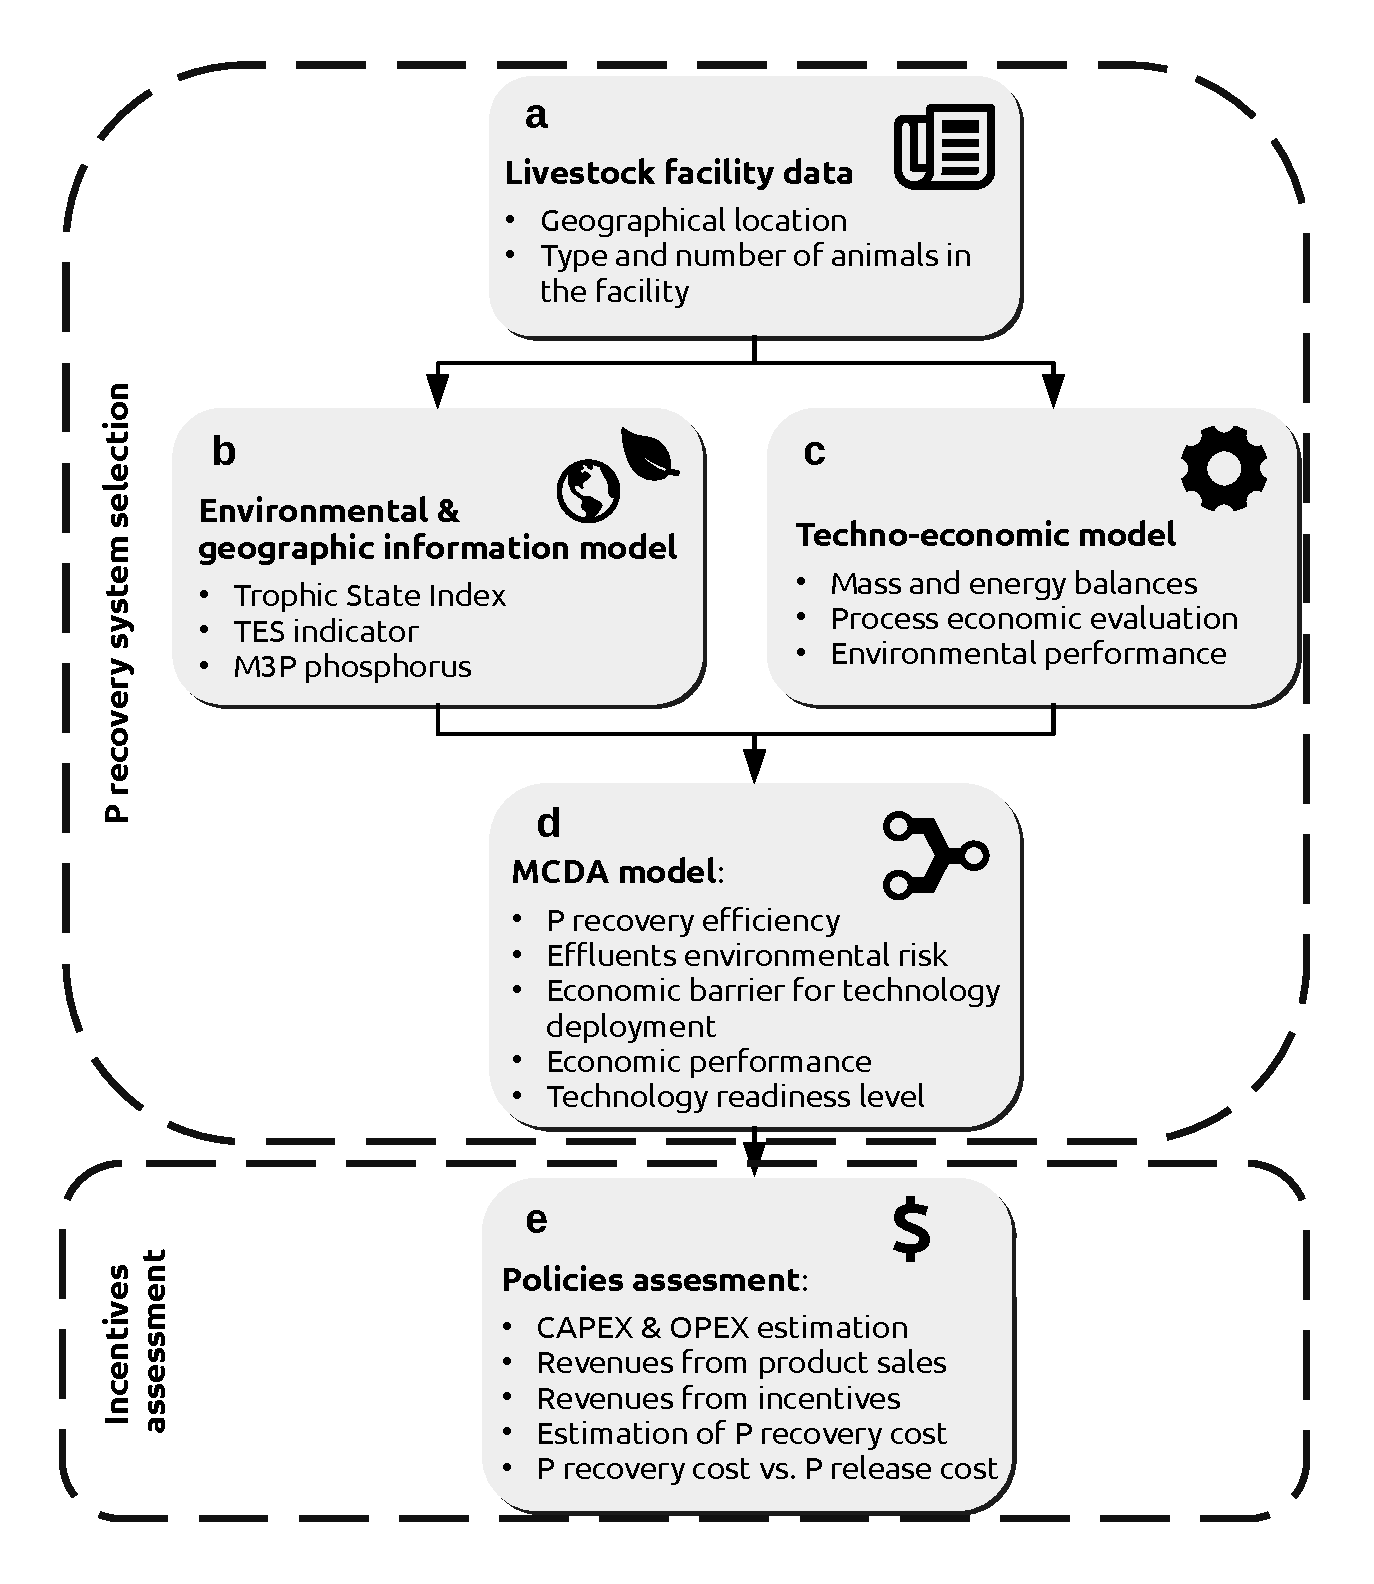
\includegraphics[width=0.7\linewidth, trim={1cm 1cm 1cm 1cm},clip]{gfx/Chapter5/tool_diagram_v4color} 
	\caption{Flowchart of the models for selection, sizing, and evaluation of nutrient recovery systems at livestock facilities.}
	\label{fig:tool_diagram}
\end{figure}

\subsection{Assessment of nutrient management systems}
Figure \ref{fig:techs_diagrams} illustrates the processes considered for livestock waste management. These processes comprise all manure treatment stages from waste collection to phosphorus recovery, including the optional biogas production stages.

\begin{figure}[h]
	\centering
	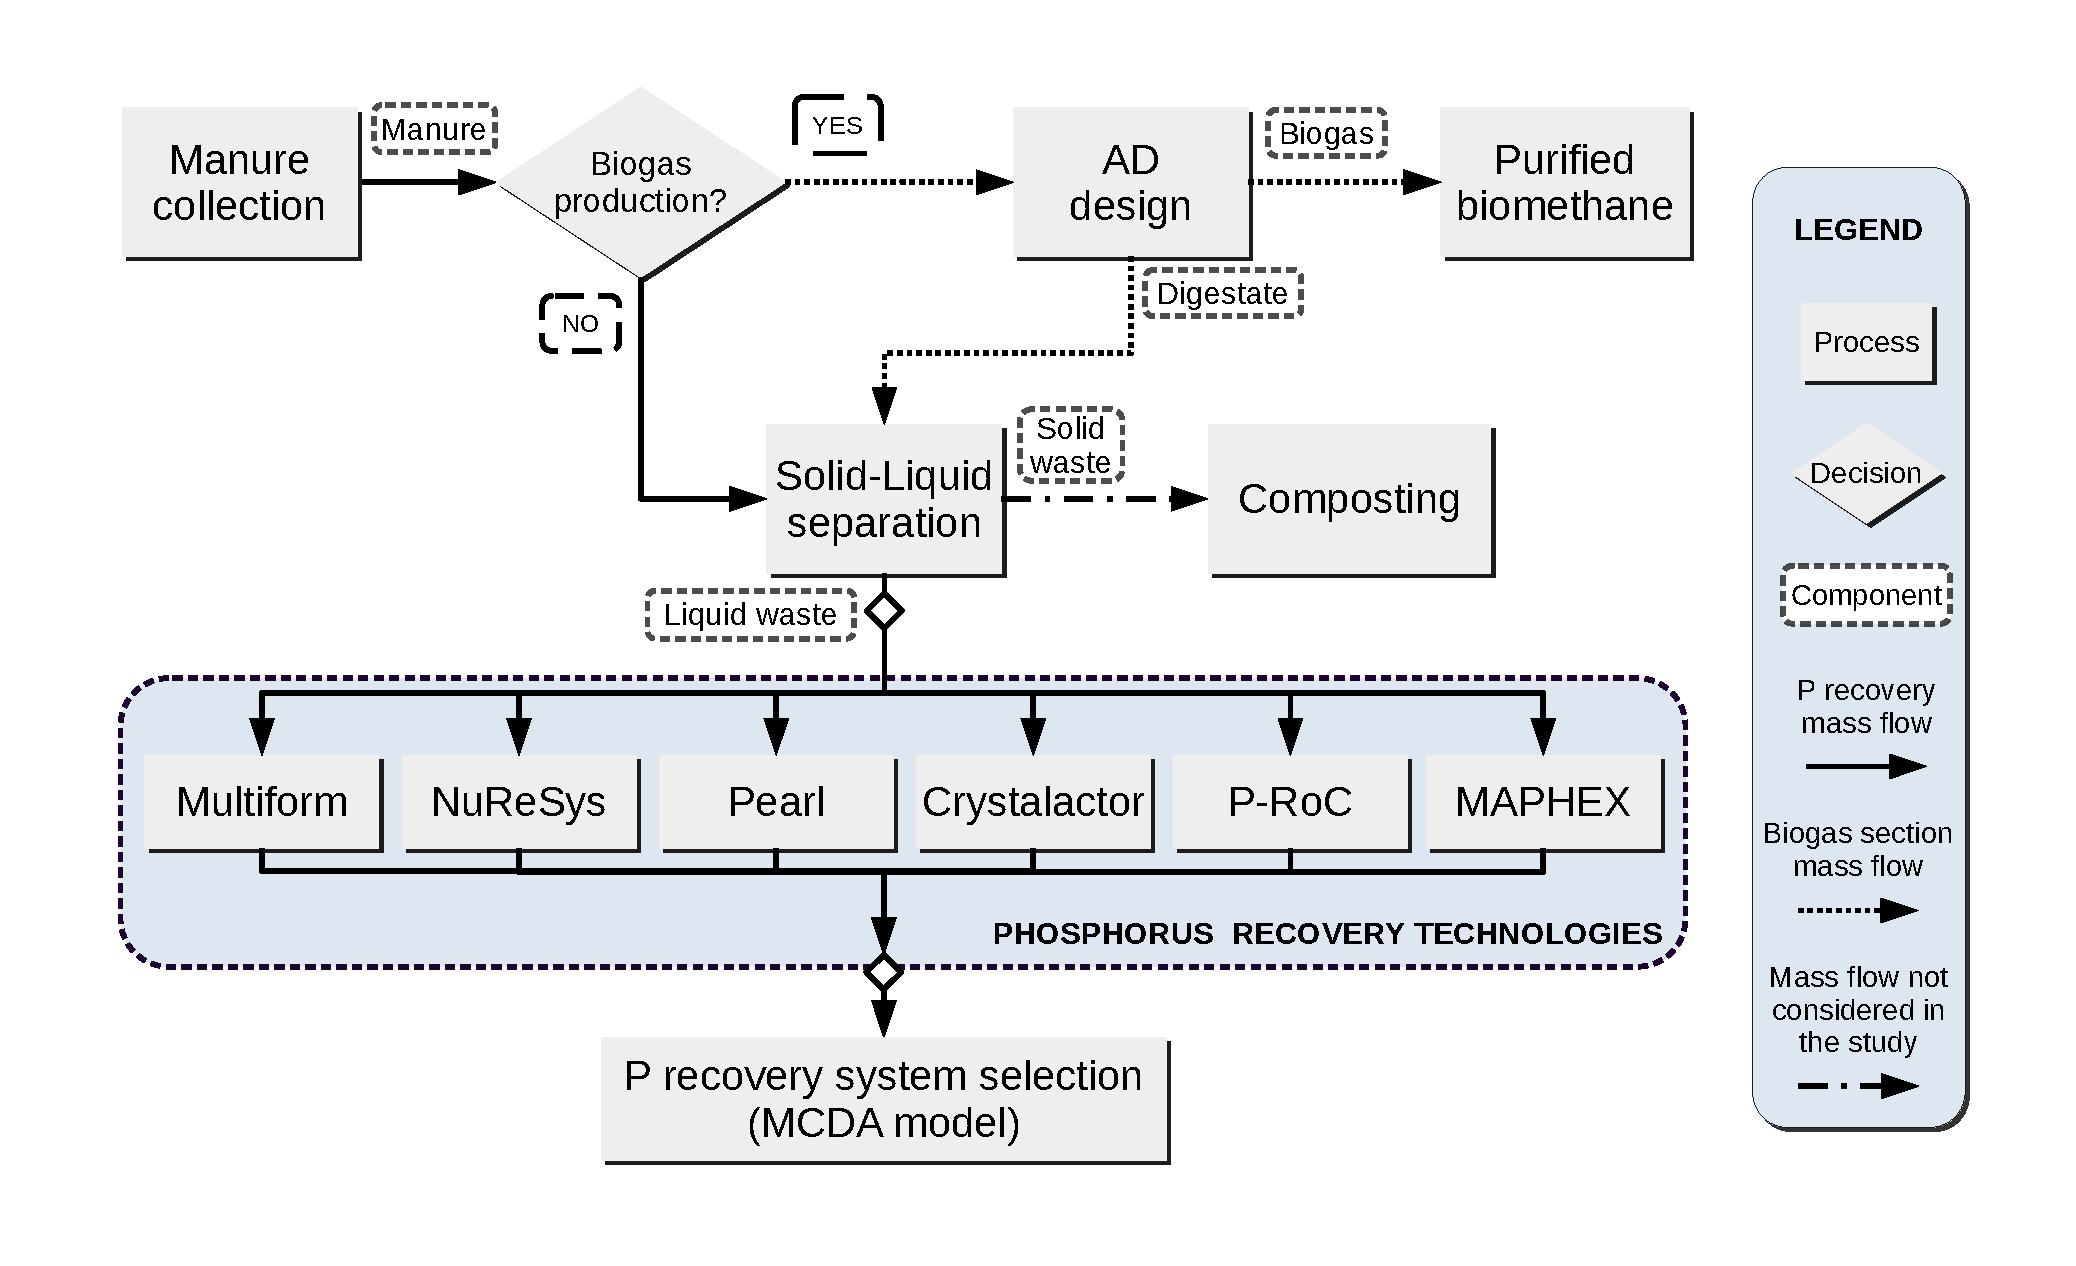
\includegraphics[width=0.85\linewidth, trim={1.5cm 1.5cm 1.5cm 1.5cm},clip]{gfx/Chapter5/Process_Flowsheet.pdf} 
	\caption{Flowchart of the processes evaluated for livestock waste management.}
	\label{fig:techs_diagrams}
\end{figure}

\subsubsection{Phosphorus recovery systems}

Six state-of-the-art technologies are assessed for phosphorus recovery at CAFOs. These technologies can be classified into three categories, i.e. struvite-based phosphorus recovery (Multiform, Crystalactor, Ostara Pearl, and NuReSys), calcium precipitates-based phosphorus recovery (P-RoC), and physical separation systems (MAPHEX). Table \ref{table:techs_description} summarizes the main parameters of the P recovery technologies assessed. The different processes, including solid-liquid separation, biogas production, and phosphorus recovery systems, are modeled based on first principles, which include mass and energy balances, thermodynamics, and product yield calculations. Additionally, data from manufacturers have been considered when available, particularly for the estimation of capital expenses (CAPEX) and operating expenditures (OPEX). A review and modeling details of the technologies considered can be found in \citet{Tool}.
%Section 2.3 of the Supplementary Information.

\begin{table}[]
	\centering
	\caption{Description of phosphorus recovery technologies considered in this work. $x_{Ca^{2+}:PO_{4}^{3-}}$ refers to the $\text{Ca}^{2+}/\text{PO}_{4}^{3-} \ \text{molar ratio}$.}
	\label{table:techs_description}
	\resizebox{\columnwidth}{!}{
		\begin{tabular}{@{}ccccc@{}}
			\toprule
			P recovery process & \begin{tabular}[c]{@{}c@{}}Technology\\ readiness level\end{tabular} & Technology type                                                                     & \begin{tabular}[c]{@{}c@{}}Phosphorus recovery\\ efficiency (\%)\end{tabular} & Reference \\ \midrule
			Multiform          & 9                          & Struvite                                                                                                & $\frac{0.798 \cdot 100}{1+\left(x_{Ca^{2+}:PO_{4}^{3-}} \cdot 0.576\right)^{2.113}}$                                   &  \citep{Pearl2Kcost2}          \\
			Crystalactor       & 9                          & Struvite                                                                                                & $\frac{0.798 \cdot 100}{1+\left(x_{Ca^{2+}:PO_{4}^{3-}} \cdot 0.576\right)^{2.113}}$                                   & \citep{egle_phosphorus_2016}          \\
			NuReSys            & 9                          & Struvite                                                                                                & $\frac{0.798 \cdot 100}{1+\left(x_{Ca^{2+}:PO_{4}^{3-}} \cdot 0.576\right)^{2.113}}$                                   &  \citep{Pearl2Kcost2}         \\
			Pearl              & 9                          & Struvite                                                                                                & $\frac{0.798 \cdot 100}{1+\left(x_{Ca^{2+}:PO_{4}^{3-}} \cdot 0.576\right)^{2.113}}$                                   & \citep{Pearl2Kcost2}           \\
			P-RoC              & 6                          & Calcium precipitates                                                                                    & 60                                   &  \citep{ehbrecht_p-recovery_2011}         \\
			MAPHEX             & 7                          & \begin{tabular}[c]{@{}c@{}}Modular system based on\\ phases separation\end{tabular}                          & 90                                   &     \citep{church_novel_2016}      \\ \bottomrule
	\end{tabular}}
\end{table}

\subsubsection{Biogas production and upgrading}
Nutrient management technologies can be implemented either as standalone systems, or integrated with biogas production and upgrading processes, being both scenarios considered in this work. In scenarios in which the integrated nutrient-energy recovery processes are considered, biogas is produced through AD of cattle waste. In a second stage, biogas impurities (mainly $\text{H}_2 \text{S}$, $\text{NH}_3$, and moisture) are eliminated, and carbon dioxide is removed using a pressure swing adsorption (PSA) unit. A detailed description for the modeling of AD and biogas purification processes can be found in \citet{Leon}. A comprehensive description for the PSA system and its modeling is shown in \citet{MartinHernandez}.

\subsection{Environmental vulnerability to nutrient pollution}
A geographic information system (GIS) model is developed to estimate the environmental vulnerability to nutrient pollution of the area where each studied CAFO is located. We have considered three dimensions of phosphorus pollution to determine the eutrophication risk in each studied watershed, (i) the average Trophic State Index (TSI) of the waterbodies in the studied area \citep{carlson_trophic_1977}, (ii) the legacy of phosphorus in soils measured by the Mehlich 3 phosphorus (M3P) concentration \citep{Espinoza2006}, and (iii) the balance between phosphorus releases and uptakes derived from human activities using the the techno-ecological synergy (TES) metric \citep{TESmetric}. These parameters have been evaluated at a sub-basin spatial scale, which corresponds to the HUC8 level defined in the Hydrologic Unit Code (HUC) system \citep{HUC8}. The information retrieved by this environmental GIS-based model is used to set the priority of environmental and economic criteria, as described in the next section. A detailed description of the GIS model used to estimate the vulnerability to nutrient pollution can be found in \citet{Tool}.
%the section 2.2 of the Supplementary Material.

\subsection{Multi-criteria decision analysis model for the assessment of nutrient management systems}
The model developed for the evaluation of on-site processes for the treatment of livestock waste is based on a multi-criteria decision analysis (MCDA) framework. This framework combines the information from the techno-economic assessment and the local environmental vulnerability to nutrient pollution. Five parameters which can be classified in three dimensions are evaluated to select the most suitable P recovery process for each CAFOs; i.e.,  (i) environmental dimension assessing the performance of the different technologies to mitigate phosphorus releases from CAFOs, which measured through the fraction of phosphorus recovered by each technology (criterion 1), and the eutrophication potential of its effluents (criterion 2), (ii) the economic performance of the P recovery systems, including the economic barrier for the implementation of P recovery processes measured in terms of capital cost (criterion 3), and the net present value (NPV) of each process (criterion 4), and (iii) the technical maturity of each system, measured through the technology readiness level (TRL) index (criterion 5).

We developed a flexible criteria aggregation method able that balances the operating cost of the systems and the P recovery efficiency as a function of the environmental vulnerability to eutrophication of each region through criteria prioritization. In order to promote the implementation of proven P recovery processes, the TRL index is set as the criteria with highest preference in all cases. Regarding the environmental and economic aspects, environmental criteria are prioritized in the MCDA module if high values for TSI or M3P are reported for the area of study, which result in severe environmental risk of phosphorus pollution. As a consequence, the selection of phosphorus recovery technologies with larger recovery efficiencies is prioritized even if they incur in larger capital or operating expenses. On the other hand, economic criteria are prioritized for technology selection either of the following situations happens, (a) if the trophic state of waterbodies is oligotrophic or mesotrophic and therefore there is no immediate eutrophication risk, but phosphorus emissions and uptakes are unbalanced, or (b) no environmental risk is reported.

For each studied CAFO, the normalized criteria are combined following the preference method described above. As a result, we obtain a composite index for each P recovery technology that collects the information of the criteria considered. 
Based on the value of this composite index, these processes can be compared and ranked, selecting the most suitable system for each studied CAFO. Detailed descriptions for the construction of composite indexes can be found in  \citet{HandbookCompositeIndicators}. 

In order to achieve a robust decision for the selection of the most adequate phosphorus recovery process, a sensitivity analysis considering different methods for the normalization and aggregation of economic and environmental information is performed \citep{MarcoCinelli2020}. A comprehensive description of the MCDA model for the selection of phosphorus recovery systems according to the economic and environmental parameters of each CAFO is collected in \citet{Tool}.
%Section 2.4 of the Supplementary Information.

\subsection{Types of incentives considered}
The implementation of nutrient recovery incentives in the form of phosphorous credits (P credits) has been studied in this work. In addition, in those scenarios where biogas production is integrated, renewable electricity certificates (REC) are also considered.

P credits can provide a mechanism to promote the recovery of phosphorus that is similar to the carbon credit scheme used in the context of carbon emissions, leading to the development of a credits market around phosphorus releases. The acquisition of P credits can bring allowances for phosphorus releases. Conversely, an entity can obtain income by recovering phosphorus releases, which is the P credits definition considered in this work. Previous efforts to determine the impact of implementing phosphorus recovery incentives for livestock waste management supply chain networks have been addressed by \citet{sampat_economic_2018}. An optimal value of 22 USD per kg of phosphorus recovered is proposed to ensure the profitability of nutrient management systems implemented at CAFOs. Additionally, since the deployment of phosphorus recovery systems results in marketable nutrient-rich products in the form of struvite, incomes from the sale of these products are included in the calculation of revenues.

REC incentives for energy recovery provide a fixed remuneration for the electricity produced, which can result in a higher transaction price of electricity to cover the extra production costs and guarantee long-term price stability. Many different REC values have been proposed by governmental organizations worlwide based on geographical factors and power production capacity \citep{Deremince}. Therefore, similar to the electricity market price, a value of 60 USD/MWh, has been considered as baseline price.

\subsection{Scenarios description}
A total of 36 scenarios combining incentives in the form of phosphorus credits (0, 1, 3, 5, 11, and 22 USD/${\text{kg}_\text{P recovered}}$) and for the production of electricity (considering final electricity prices of 30, 60, 75, 90, and 120 USD/MWh) are evaluated for the implementation of nutrient management systems at 2,217 CAFOs in the Great Lakes area. The base value assumed for P credits is 22 USD per kg of phosphorus recovered, based on the work of \citet{sampat_economic_2018}. Although this reference value is comparatively large with respect to the price of phosphorus in commercial fertilizer, 1.23 USD/kg P \citep{fertilizers_price}, we note that it is significantly lower than the economic losses due to the environmental and social impact of nutrient pollution, estimated to be 74.5 USD per kg of P released \citep{Sampat2020}. Regarding RECs, an average electricity market price of 60 USD/MWh has been selected as the base-scenario. An electricity price below this value, 30 USD/MWh, and three values above the electricity market price, 75, 90, and 120 USD/MWh have been considered. These high REC values are studied due to the need of large incentives for biogas facilities to be economically viable reported by \citet{sampat_economic_2018}.

We note that there are two special cases among the scenarios assessed. For those scenarios where P credits are 0,the only income of phosphorus recovery is from the sales of marketable nutrient-rich products in the form of struvite, in addition to the incomes from electricity generated if the corresponding technologies are selected. For those scenarios with an electricity price of 0 USD/MWh, no biogas production and upgrading process is implemented, considering only incomes associated with P credits and struvite sales are considered.

\subsection{Study Region - The Great Lakes area}
The Great Lakes area, shown in Figure \ref{fig:states}, is considered to study the effect of different incentive policies on P recovery processes. This region collects several factors which make it specially vulnerable to nutrient pollution originated from livestock waste. First, it has a considerable amount of CAFOs, resulting in the generation of large amounts of organic waste. Second, the fresh waterbodies in the region are key resources, accounting for 21\% of the global freshwater supply \citep{freshwater_Great_Lakes}, providing habitat to a wide range of fauna, and contributing to the local economy through recreational activities. Finally, there exists a continuous increase of cyanobacteria and HABs since the 1960s, especially in the Lake Erie, which is the shallowest lake.

\begin{figure}[h]
	\centering
	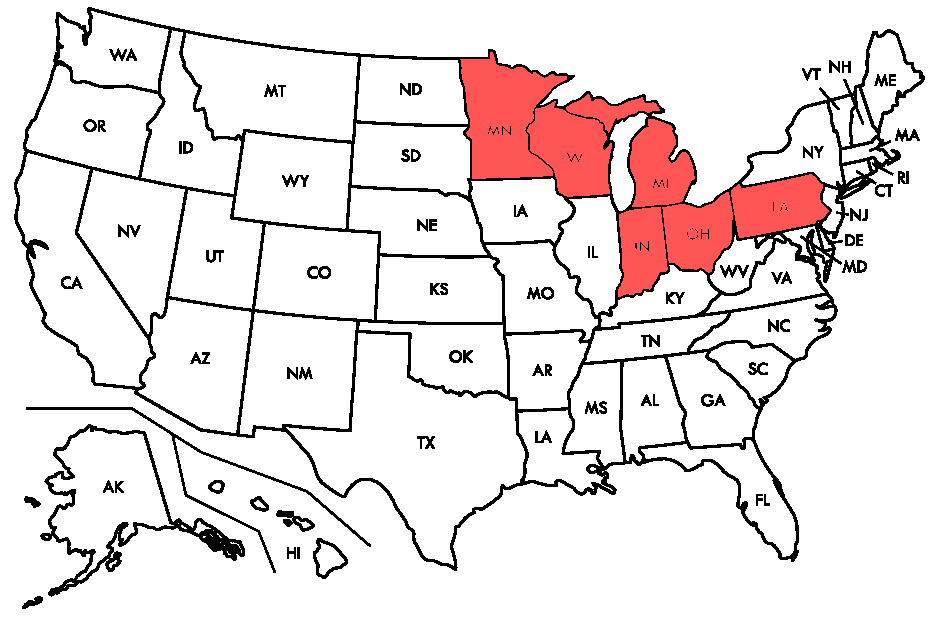
\includegraphics[width=0.65\linewidth, trim={0cm 0cm 0cm 0cm},clip]{gfx/Chapter5/Blank_US_map_borders_labels.pdf} 
	\caption{States of the Great Lakes region studied in this work.}
	\label{fig:states}
\end{figure}

The CAFOs considered for the deployment of livestock waste treatment processes are those livestock facilities with more than 300 animal units \citep{CAFO_definition} reported in the National Pollutant Discharge Elimination System (NPDES) by the US EPA in the Great Lakes area (i.e. Minnesota, Indiana, Ohio, Pennsylvania, Wisconsin, and Michigan). An animal unit is defined as an animal equivalent of 1,000 pounds live weight \citep{animal_unit_definition}. There are 2,217 CAFOs considered in total. The states of Illinois and New York, as well as the Ontario province in Canada, are not part of this study due to the lack of reliable data about CAFOs. The animal number, manure generated, and phosphorus releases by CAFOs in the studied states are reported in Table \ref{table:GreatLakes_manure}.

\begin{table}[h]
	\centering
	\caption{Livestock residues and phosphorus releases by CAFOs in the Great Lakes area.}
	\label{table:GreatLakes_manure}
	\resizebox{\columnwidth}{!}{
		\begin{tabular}{@{}ccccccc@{}}
			\toprule
			& Pennsylvania & Ohio     & Indiana  & Michigan & Minnesota & Wisconsin \\ \midrule
			Number of CAFOs & 131 & 53 & 119 & 144 & 1,487 & 283 \\
			\midrule
			Total animal units                                                                      & 196,617      & 128,008  & 187,355  & 354,460  & 943,094   & 744,015   \\ 
			Dairy animal units (\%)                                                                 & 85.06       & 79.17  & 81.93  & 87.90  & 45.43   & 98.38   \\
			Beef animal units (\%)                                                                  & 14.94       & 20.83   & 18.07   & 12.10   & 54.57   & 1.62    \\
			
			\midrule
			
			\begin{tabular}[c]{@{}c@{}}Manure generated\\ (kt/year)\end{tabular}                    & 2.60$\cdot 10^3$     & 1.68 $\cdot 10^3$ & 2.48$\cdot 10^3$ & 4.76$\cdot 10^3$ & 1.13$\cdot 10^{4}$  & 1.03$\cdot 10^{4}$  \\
			
			\midrule
			
			\begin{tabular}[c]{@{}c@{}}Phosphorus releases\\ (t/year)\end{tabular}                 & 2.08$\cdot 10^3$     & 1.34$\cdot 10^3$ & 1.98$\cdot 10^3$ & 3.80$\cdot 10^3$ & 9.02$\cdot 10^3$  & 8.20$\cdot 10^3$  \\ 		
			
			\midrule
			
			\begin{tabular}[c]{@{}c@{}}Reference\end{tabular}                 & 1     & 2 & 3 & 4 & 5  & 6  \\ 			
			\bottomrule
	\end{tabular}}
	\begin{tablenotes}
		\small
		\item \textsuperscript{1} \protect\citep{Pennsylvania_CAFOS}
		\item \textsuperscript{2} \protect\citep{Ohio_CAFOS}
		\item \textsuperscript{3} \protect\citep{Indiana_CAFOS}
		\item \textsuperscript{4} \protect\citep{Michigan_CAFOS}
		\item \textsuperscript{5} \protect\citep{Minnesota_CAFOS}
		\item \textsuperscript{6} \protect\citep{Wisconsin_CAFOS}
	\end{tablenotes}
\end{table}

\section{Results and discussion}
\subsection{Single incentives}
In this section, the effect of the implementation of single P credits or REC incentives is studied. The capital and operating costs associated with the installation of P recovery systems if no incentives are considered are reported \citet{Tool}.
%in Table 13S of the Supplementary Material.

\subsubsection{Effect of P credits}
The effect of applying P credits on the economic performance of nutrient management systems has been studied. Revenues from struvite sales are also considered in those CAFOs installing struvite production technologies. Since in this first scenario only the effect of P credits is studied, incomes from electricity production are excluded; and therefore, the nutrient management systems are not integrated with biogas production. The effect of the value of P credits over the profitability of the nutrient recovery systems is shown in Fig \ref{fig:NoREC}, where the distribution of CAFOs size is shown using boxplots. It can be observed that, for P credits values strictly below 11 USD per kg of recovered phosphorus, the proportion of profitable P recovery processes (those installed processes whose incomes are larger than the operating expenses) is small and constant. However, when the value of the incentive is set at 11 USD per kg of recovered phosphorus, the increase in the number of profitable processes is very significant for all states except Minnesota, which CAFOs median size is the smallest. For states with large CAFOs, i.e. Michigan, Ohio and Wisconsin, the percentage of profitable processes can reach around 80\% under high P credits; while for Indiana and Pennsylvania, with medium-size CAFOs, around 40\% are profitable. For P credits of 22 USD per kg of recovered phosphorus, there is an additional 25\% increase of profitable nutrient recovery systems in those states with large CAFOs. In the states with medium size CAFOs the increase of profitable processes is also very significant, reaching approximately 80\% of the studied CAFOs. Finally, for the case of Minnesota, there is a large increase in the profitable P recovery systems installed as well, reaching near the 60\% of the CAFOs studied.

\begin{figure}[h]
	\centering
	\begin{subfigure}[t]{0.49\textwidth}
		\centering
		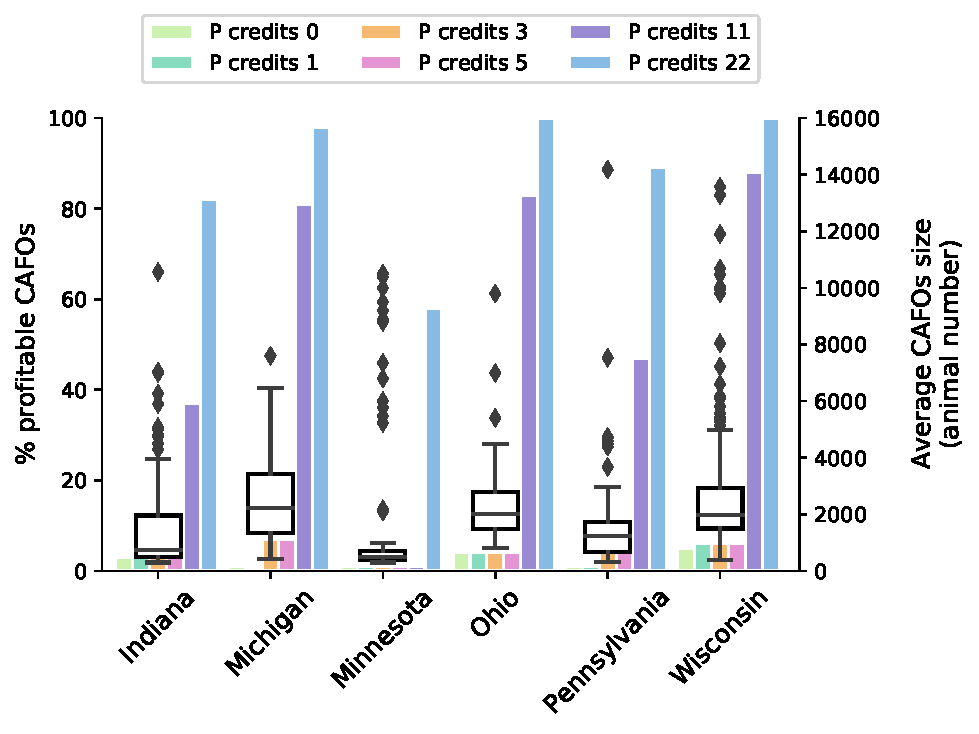
\includegraphics[width=\linewidth]{gfx/Chapter5/REC0DataAnalysis__PercProfitableStates.pdf} 
		\caption{P credits $\left(\frac{\text{USD}}{\text{kg}_\text{P recovered}}\right)$}
		\label{fig:NoREC}
	\end{subfigure}
	\begin{subfigure}[t]{0.49\textwidth}
		\centering
		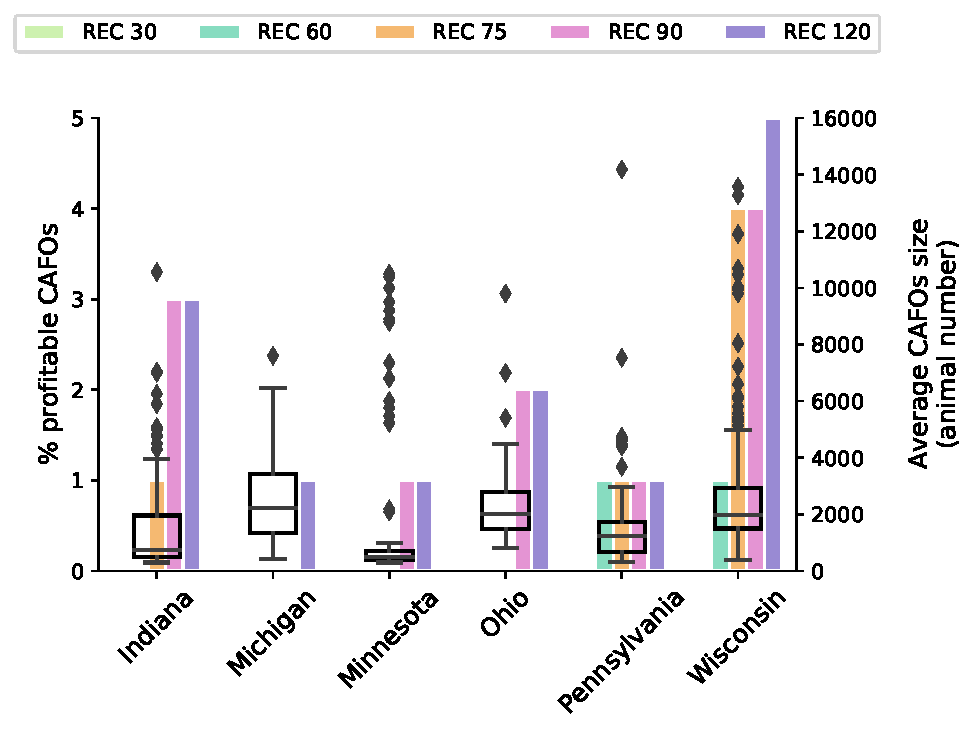
\includegraphics[width=\linewidth]{gfx/Chapter5/PC0DataAnalysis__PercProfitableStates.pdf}
		\caption{REC $\left(\frac{\text{USD}}{\text{MWh}}\right)$}
		\label{fig:NoPCredits}
	\end{subfigure}
	
	\caption{Distribution of profitable phosphorus recovery processes in the Great Lakes area for the scenarios considering phosphorus credits and renewable energy credits. The box-plots represent the distribution of CAFOs size in each state.}
	\label{fig:SingleIncentives}
\end{figure}

\subsubsection{Effect of renewable energy certificates}\label{section:Electricity_price}
The effect of REC in the implementation of P recovery systems is studied in this section. Integration of biogas production with P recovery processes is considered in all the cases studied in this scenario. In addition to revenues obtained from RECs, incomes from the sales of struvite produced by the phosphorus recovery processes have been considered as well. The effect of P credits is excluded in this scenario.

Figure \ref{fig:NoPCredits} shows the percentage of profitable P recovery processes for each studied state together with the distribution of the size of CAFOs. As it can be observed, the impact of the incomes from electricity in the economic performance is much less significant than the effect of P credits given the incentive ranges considered. Only the largest CAFOs, most of which represent outliers in the distribution of CAFOs size, are profitable when prices equal to or above 75 USD/MWh are considered. The large CAPEX prevent the economic feasibility of biogas production in small and medium CAFOs. Therefore, only large-scale CAFOs can benefit from the operation of biogas processes to cover the cost of P recovery systems via biogas-based electricity production.

\subsection{Combined effect of incentives for phosphorus and renewable electricity recovery}\label{section:CombIncent}
Synergies derived from the combination of P credits and RECs might be obtained when integrating phosphorus recovery technologies with biogas production and upgrading processes.
However, since the deployment of the biogas processes involves large investments and considerable operating costs, a detailed analysis must be conducted to identify the most cost-effective incentives policy. 

The results obtained from combining the incentive schemes described in previous sections are shown in Figure \ref{fig:AllScenarios}. The fraction of profitable processes is shown in Figure \ref{fig:PercProfitableStates_AllScenarios}, which are defined as those CAFOs with positive net incomes. It can be observed that, if the value of P credits and RECs are set similar to the market prices (i.e. 1 USD/$\text{kg}_\text{P recovered}$ and 60-75 USD/MWh respectively), the fraction of profitable processes is very low. Wisconsin is the state with the largest share of profitable P recovery processes under this scenario, which is 4-5\% of the total CAFOs.

Phosphorus credits have a larger impact on the profitability of nutrient management systems, near to 100\% for P credits of 22 USD/${\text{kg}_\text{P recovered}}$ for states with large CAFOs (i.e. Michigan, Ohio and Wisconsin). The price of electricity has a weak influence on the profitability of the deployed systems in these scenarios. For states with medium-size CAFOs, Indiana and Pennsylvania, the share of profitable processes is around 80-85\%. For Minnesota, which is the state with the smallest median CAFOs size, the share is 58\%. Therefore, the installation of AD processes has a significantly negative impact in the states with small and medium size CAFOs due to the lack of economies of scale. A similar behavior is found when the value of phosphorus credits is reduced to 11 USD/${\text{kg}_\text{P recovered}}$.

This pattern is reverted when P credits of 3-5 USD/${\text{kg}_\text{P recovered}}$ are considered. For these scenarios the share of profitable processes is considerably reduced compared to the previous scenarios. Actually, for Indiana, Minnesota, and Ohio, there is no difference between setting phosphorus credits incentives below 5 USD/${\text{kg}_\text{P recovered}}$ and the case considering no P credits (where the only income of phosphorus recovery is from the sales of nutrient-rich products obtained). However, in all states except Minnesota, the amount of profitable systems increases for electricity prices larger than 60 USD/MWh, reaching a share of P recovery processes with positive net incomes up to 22 \% for Michigan. For the scenario considering P credits of 1 USD/${\text{kg}_\text{P recovered}}$, only Ohio shows a slight improvement in the fraction of profitable facilities if the production of electricity is also considered. Therefore, there is a threshold for P credits between 1 and 3 USD/$\text{kg}_\text{P recovered}$ below which no improvement in the fraction of profitable P recovery systems is observed. For those scenarios where no incentive for phosphorus recovery is considered, the results obtained have been previously described in Section \ref{section:Electricity_price}. It is interesting to note, as a consequence of the large capital and operating expenses of AD processes, the economic performance of the scenarios considering only P recovery systems is at least as profitable as the profitability of the scenarios considering biogas generation associates the largest REC incentives.

The net treatment cost per ton of manure processed captures the perspective of CAFOs owners on P recovery. It is defined as the difference between the revenues (sum of struvite sales, $R_{c}$ (USD/year), and incentives, $I_{c}$ (USD/year)) and the operating expenditures of livestock treatment processes, $OPEX_{c}$ (USD/year), as shown in Eq. \ref{eq:NetTreatCost}. $F_{\text{manure}_{c}}$ denotes the mass flow of manure processed in ton/year.

\begin{align}
& \text{Net treatment cost}_c \left(\frac{\text{USD}}{\text{t}_{\text{manure}}}\right) = \frac{R_{c} + I_{c} - OPEX_{c}}{F_{\text{manure}_{c}}} \label{eq:NetTreatCost}
\end{align}

\begin{figure}[h!]
	\centering
	\begin{subfigure}[t]{0.89\textwidth}
		\centering
		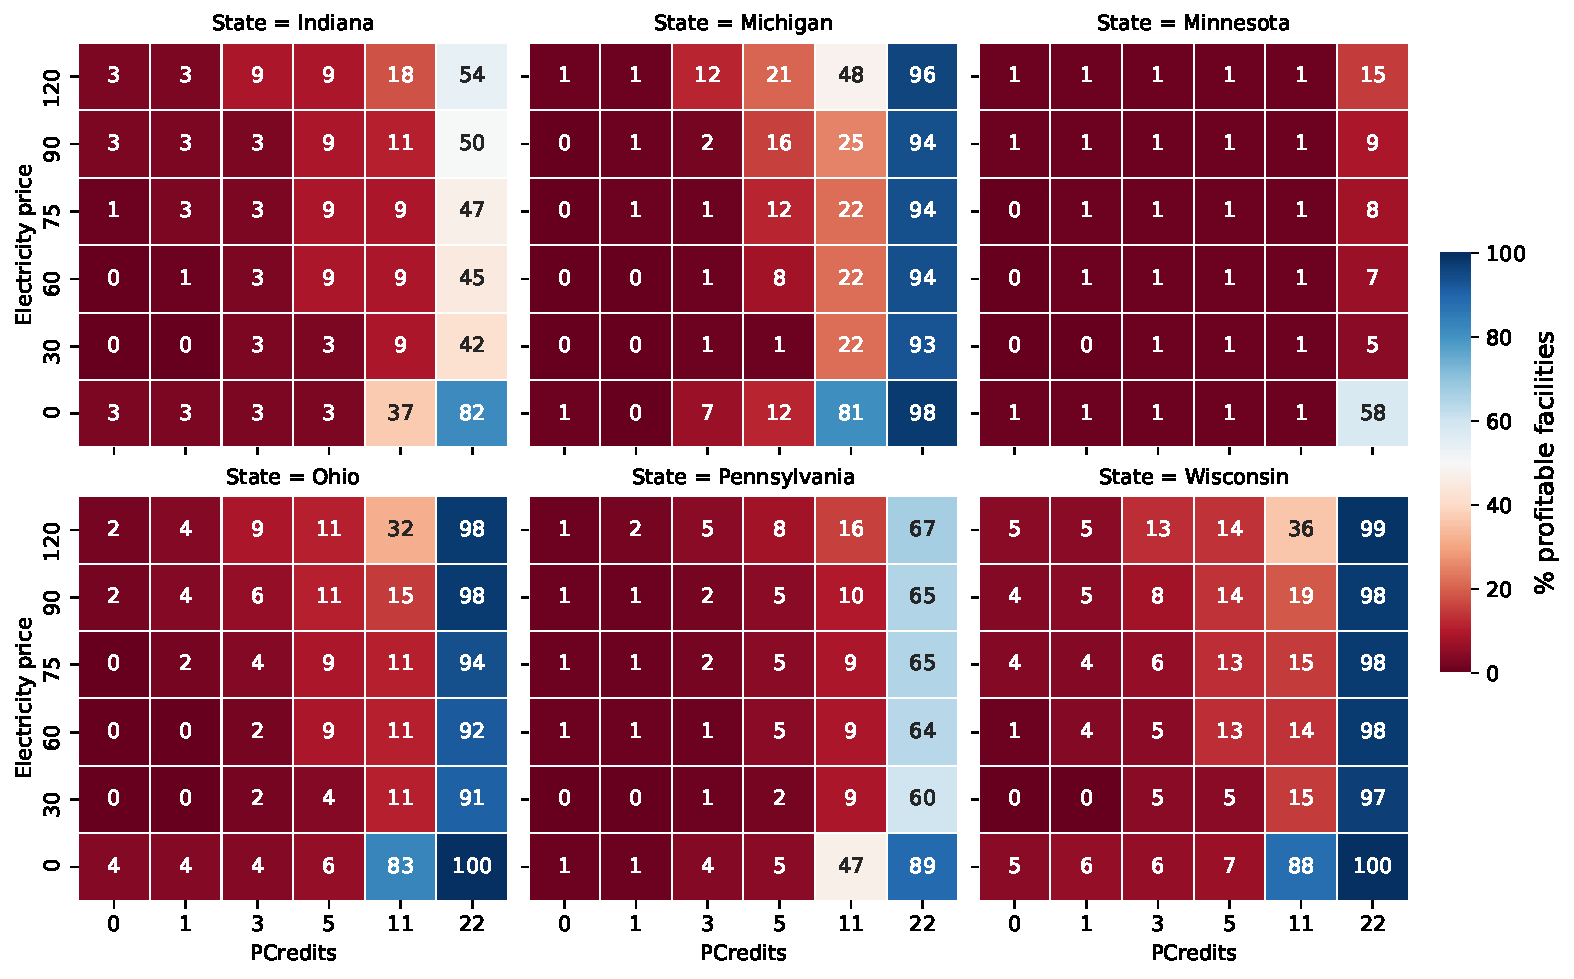
\includegraphics[width=\linewidth]{gfx/Chapter5/DataAnalysisProfitable.pdf} 
		\caption{Percentage of profitable phosphorus recovery processes}
		\label{fig:PercProfitableStates_AllScenarios}
	\end{subfigure}
	\par\bigskip
	\begin{subfigure}[t]{0.89\textwidth}
		\centering
		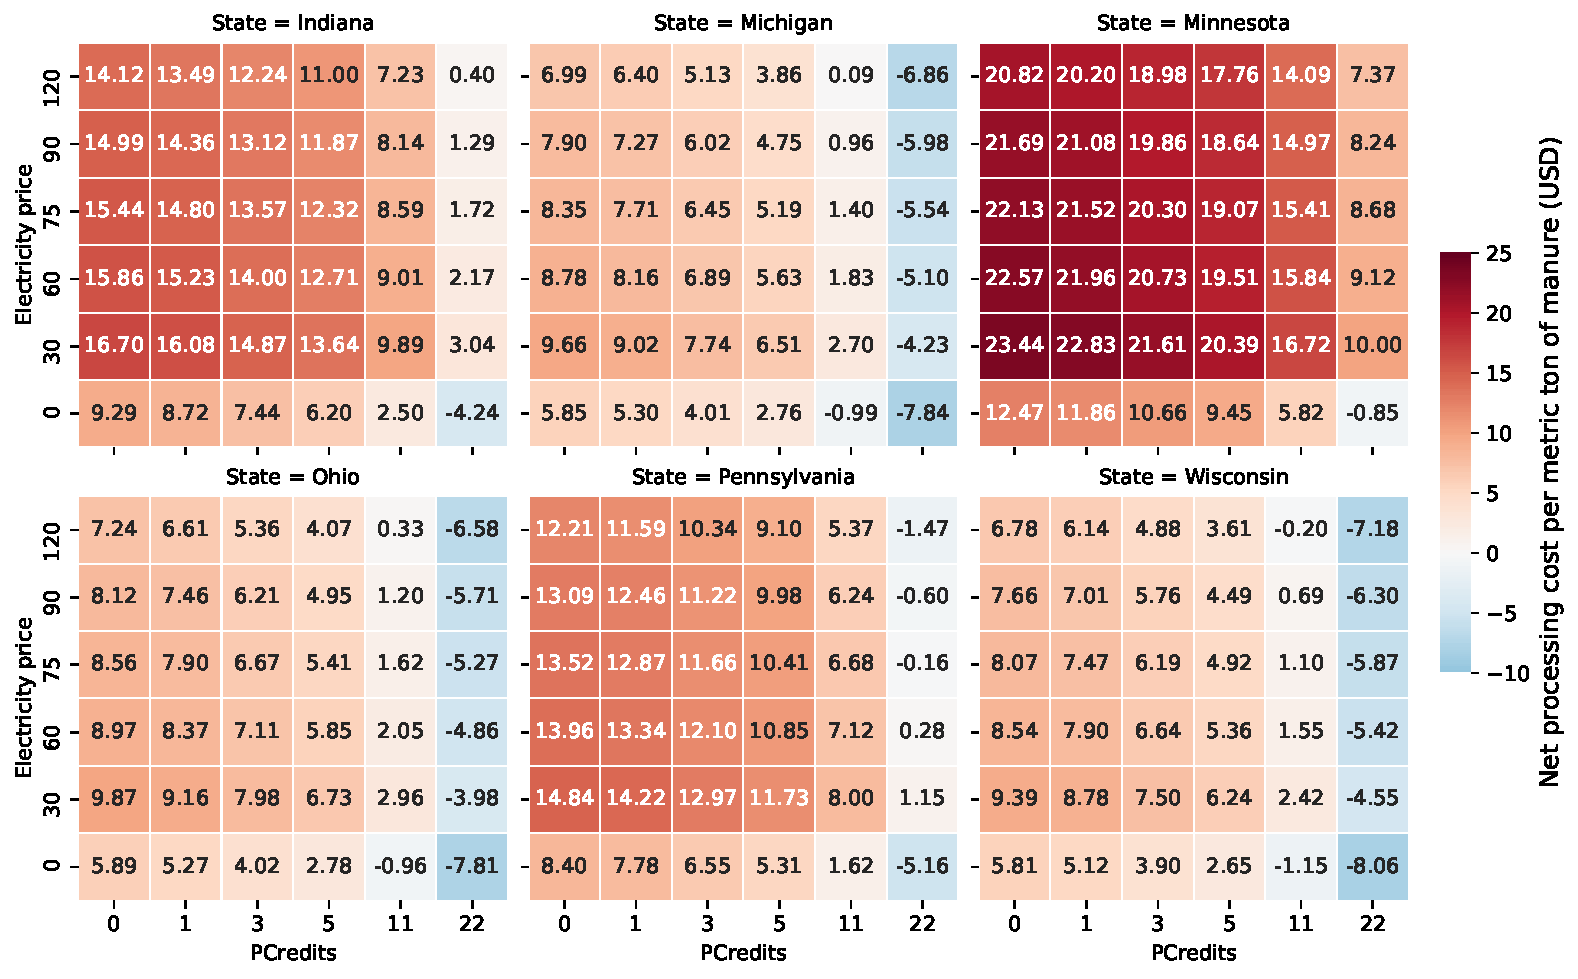
\includegraphics[width=\linewidth]{gfx/Chapter5/TAC_tonManure.pdf}
		\caption{Net processing cost per metric ton of manure (USD)}
		\label{fig:TAC_kgManure_AllScenarios}
	\end{subfigure}
	
	\caption{Economic evaluation of P recovery processes for the different incentives scenarios studied}
	\label{fig:AllScenarios}
\end{figure}

The results obtained in terms of net treatment cost are illustrated in Figure \ref{fig:TAC_kgManure_AllScenarios}. These  show a base cost for the recovery of phosphorus between 5.81 and 12.47 USD per ton of processed manure if no incentives or anaerobic digestion stages are considered. From this base case, it can be observed that the costs vary following the same pattern as the fraction of profitable processes described previously. The installation of biogas processes is not profitable by itself, increasing the processing costs by 1.2-1.9 times over the base case if no P credits are considered, and it is only beneficial for specific scenarios which have large size CAFOs, and moderate P credits ($>$3 USD/${\text{kg}_\text{P recovered}}$) and electricity incentives ($>$60 USD/MWh). The scenarios combining states with large CAFOs and high value for P credits, and the optional production of renewable energy from biogas result in negative processing costs. This means that phosphorus recovery results in profits for the CAFO. We note that, as the analysis of the different scenarios is carried out at the state level, a negative processing cost indicate that, under certain schemes for incentives, the profitable P recovery processes are able to balance out the non-profitable ones in the state.

It is worth noting that the results reveal that in the largest CAFOs the recovery of phosphorus is more feasible, due to the economies of scale. At the same time, however, these large-scale CAFOs also represent the major environmental threats due to the release of larger amounts of phosphorus.

\subsection{Environmental cost-benefit analysis}
CAFOs are an environmental concern in terms of nutrient pollution as a consequence of the high spatial concentration of animals, resulting in large releases of phosphorus. 
The long-term environmental impact of phosphorus releases result in large economic losses, accounting for the remediation cost of environmental degradation and the economic impact on the local population affected by HABs. Therefore, an analysis for the cost-effectiveness of the total cost involved in phosphorus recovery, including the amortization of the investment, operating costs, and total cost of incentives, can show the economic advantages of phosphorus recovery. 

\begin{align}
& \text{Total treatment cost}_{c} \left(\frac{\text{USD}}{\text{kg}_{\text{P recovered}}}\right) = R_{c} + I_{c} + OPEX_{c} \label{eq:TotTreatCost}
\end{align}

Figure \ref{fig:plot_scenarios} shows the total cost of phosphorus recovery under different policies, defined in Eq. \ref{eq:TotTreatCost}, compared with the economic losses due to phosphorus releases into the environment. It can be observed that all scenarios studied result in a phosphorus recovery cost lower than the economic looses due to phosphorus releases, estimated in 74.5 USD per kg of phosphorus released by \citet{Sampat2020}. Phosphorus recovery is, therefore, more cost-effective than its release to the environment. The lowest total cost for phosphorus recovery is obtained in the scenario not involving any incentive (\textit{REC: 0 - PC: 0}), resulting in costs between 3 and 5 times lower than the economic cost of phosphorus release to the environment. The application of incentives increases the total monetary cost of phosphorus recovery, mainly driven by the application of phosphorus credits. However, since incentives are an income for the owners of livestock facilities, the economic cost of nutrient management systems for the owners of CAFOs is progressively reduced, increasing the number of profitable P recovery systems, and reducing the recovery cost of phosphorus, as it is shown in Fig. \ref{fig:AllScenarios}.

\begin{figure}[h!]
	\centering
	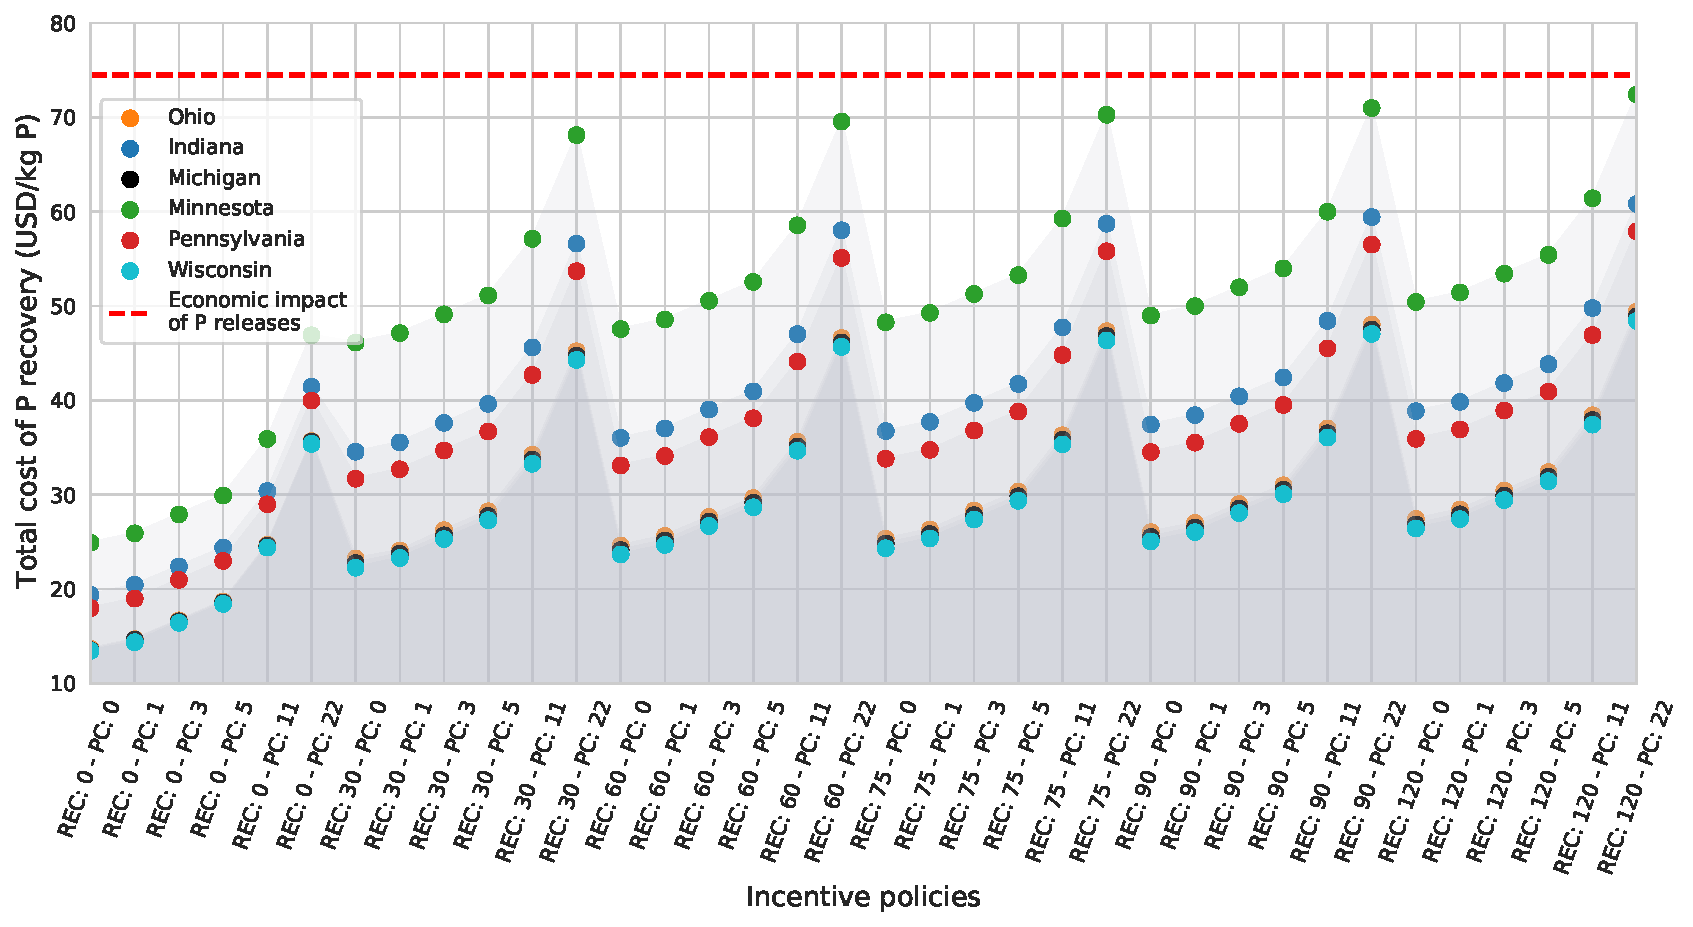
\includegraphics[width=\linewidth]{gfx/Chapter5/TotalCost_kgPRecoveredAllStatesv2.pdf} 
	
	\caption{Comparison of the total cost of phosphorus recovery for each scenario assessed and the environmental remediation cost due to phosphorus releases. \textit{REC} denotes the electricity incentive values considered in USD/MWh, and \textit{PC} denotes the value of phosphorus credits in USD/${\text{kg}_\text{P recovered}}$. The red dotted line represents the economic losses due to phosphorus releases to the environment.}
	\label{fig:plot_scenarios}
\end{figure}

The role of the size of CAFOs in the cost of phosphorus recovery can be also observed in this study. Accordingly with the results shown in previous sections, those states with larger average size of CAFOs, such as Wisconsin, Ohio, and Michigan, have recovery costs significantly lower than the states where medium and small size CAFOs are predominant. It is worth noting that the total cost of phosphorus recovery is lower than the economic losses due to the release of phosphorus to the environment for all the evaluated states and policies.

\subsection{Fair distribution of incentives}
The effect of different incentive schemes has been previously discussed, revealing that the P recovery systems in small CAFOs require significant economic support in the form of incentives to balance the monetary looses, while in the largest CAFOs these systems can be self-profitable. This situation leads to the problem of the fair distribution of available incentives, which is particularly relevant in the case that the available budget is not sufficient to cover the operating expenses of the unprofitable P recovery processes. In this section, the minimum necessary incentives for all P recovery systems in the studied area to reach the economical neutrality (i.e., no economic profits or looses are obtained) is firstly determined. In a second stage, a fairness-guided distribution of incentives among CAFOs is studied when the available incentives are lower than the monetary amount determined, i.e., they are not sufficient to cover the operating expenses of unprofitable processes. Due to the marginal benefits obtained by installing AD processes, as described in Section \ref{section:CombIncent}, the implementation of only P recovery systems is assumed in both studies, and therefore only incentives for P recovery are considered.

The minimum cost of incentives necessary for covering the economic losses of unprofitable processes, estimated in 222.6 million USD, is determined through the formulation of an optimization problem. The objective function of this problem minimizes the incentives used, Eq. \ref{eq:objMinIn}, subject to achieve the economical neutrality, Eq. \ref{eq:cons1MinIn}. Here, $\mathcal{C}$ denotes the set of CAFOs studied, $I_{c}$ the  incentives allocated, and $OPEX_{c}$ and $R_{c}$ the operating expenses and revenues of the P recovery system installed in each CAFO $c$ respectively.

\begin{subequations}
	\begin{align}
	& \text{min} \ \ \sum_{c \in \mathcal{C}} I_{c}  \label{eq:objMinIn} \\
	& \text{s.t.} \ \ I_{c} + R_{c} - OPEX_{c} \geq 0 \label{eq:cons1MinIn}
	\end{align}
\end{subequations}

The results obtained, shown in Figure \ref{fig:MinIncent}, reveal the crucial role of the economies of scale in the amount of incentives that must be deployed to cover the economic looses of P recovery systems. We note that the discrepancies of incentives for CAFOs of similar size that can observed in the figure are due to different technology installed. The selection of different P recovery processes for CAFOs of similar size is based on the eutrophication risk of each watershed, 
as described in \citet{Tool}.
%see Section 2.4 of the Supplementary Material. 
It can also be observed the 99.9\% of CAFOs require incentives below the P releasing cost to the environment. A correlation to estimate the amount of incentives needed to cover the operating expenses as a function of CAFOs capacities is proposed in Eq. \ref{eq:CorrMinIn} , where $AU_{c}$ denotes the animal units of CAFO $c$.

\begin{align}
& I_{c} \ \left(\frac{\text{USD}}{\text{kg P}}\right) = \frac{3.383 \cdot 10^6}{1+\left(AU_{c} \cdot 2.223\cdot 10^5 \right)^{0.647}} \label{eq:CorrMinIn} 
\end{align}

\begin{figure}[h!]
	\centering
	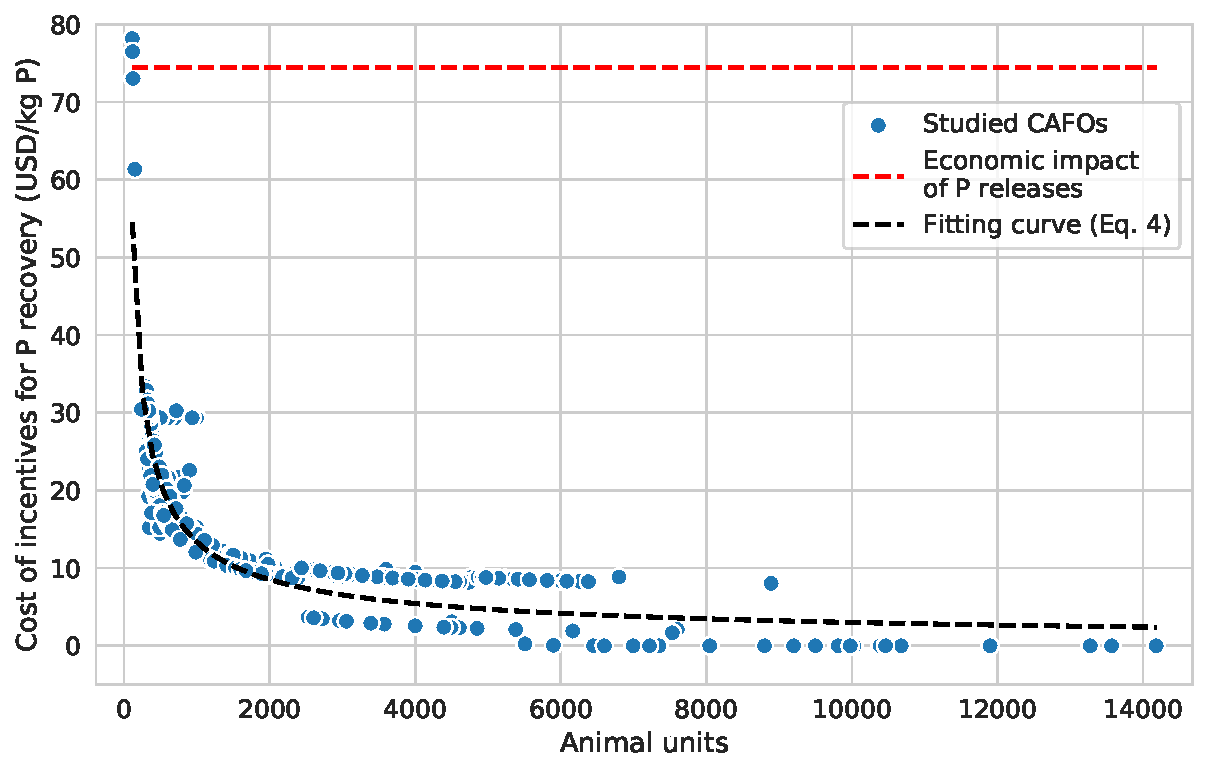
\includegraphics[width=0.7\linewidth, trim=0cm 0cm 0cm 0cm, clip]{gfx/Chapter5/MinIncent.pdf}
	\caption{Allocation of incentives for achieving the economic neutrality of nutrient recovery systems minimizing the total cost of incentives.}
	\label{fig:MinIncent}
\end{figure}

The fair allocation of incentives when the monetary amount available is not sufficient to cover the expenses of all P recovery processes has been addressed by using the Nash allocation scheme. The Nash approach has been selected because this scheme is able to capture the scales of the different stakeholders (CAFO facilities) in order to achieve a fair distribution of a certain resource (incentives), as it was demonstrated by \citet{sampat2019fairness}. This scheme is formulated in Eqs. \ref{eq:objNashIn}-\ref{eq:cons1NashIn}, where $I_{\text{available}}$ denotes the available incentives.

\begin{subequations}
	\begin{align}
	& \text{max} \ \ \sum_{c \in \mathcal{C}} \text{ln} \left(I_{c} + R_{c} - OPEX_{c}\right)  \label{eq:objNashIn} \\
	& \text{s.t.} \ \ \sum_{c \in \mathcal{C}} I_{c} \leq I_{\text{available}} \label{eq:cons1NashIn}
	\end{align}
\end{subequations}

\begin{figure}[h!]
	\centering
	\begin{subfigure}[t]{0.89\textwidth}
		\centering
		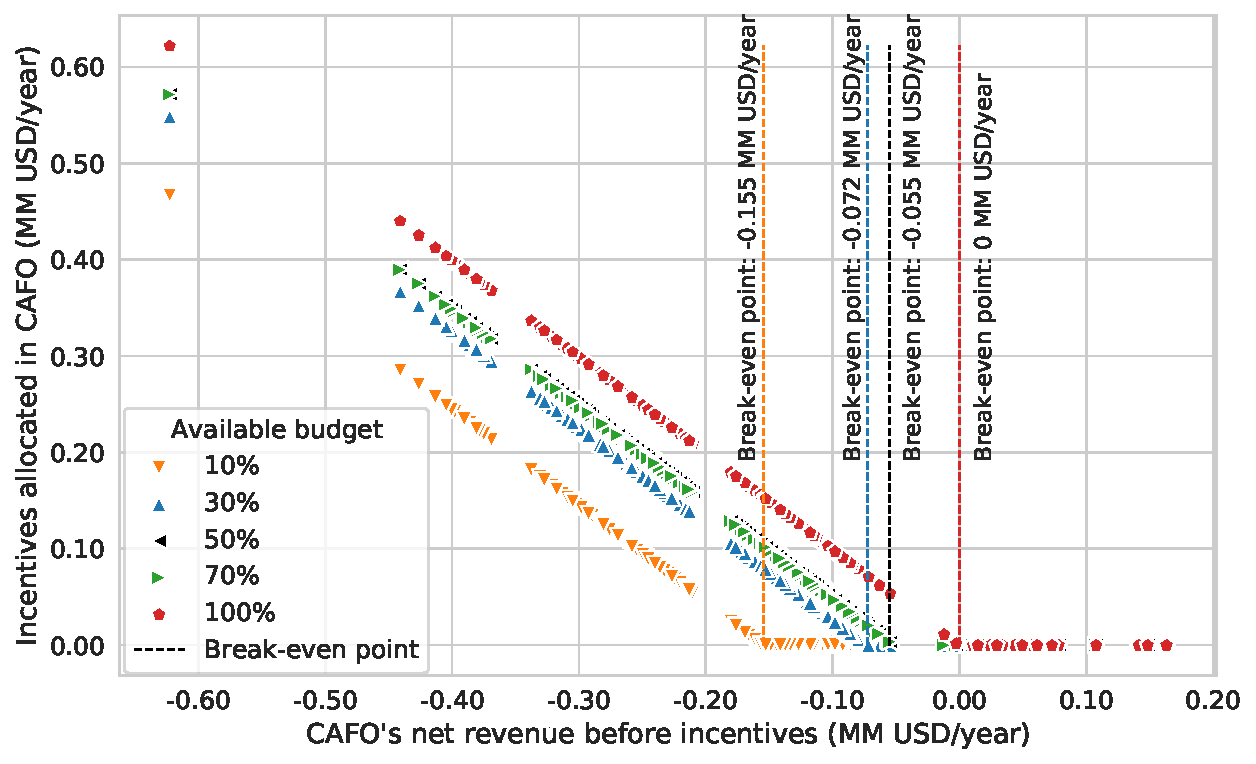
\includegraphics[width=\linewidth]{gfx/Chapter5/NashIncent.pdf} 
		\caption{Distribution of incentives}
		\label{fig:NashIncent}
	\end{subfigure}
	\par\bigskip
	\begin{subfigure}[t]{0.89\textwidth}
		\centering
		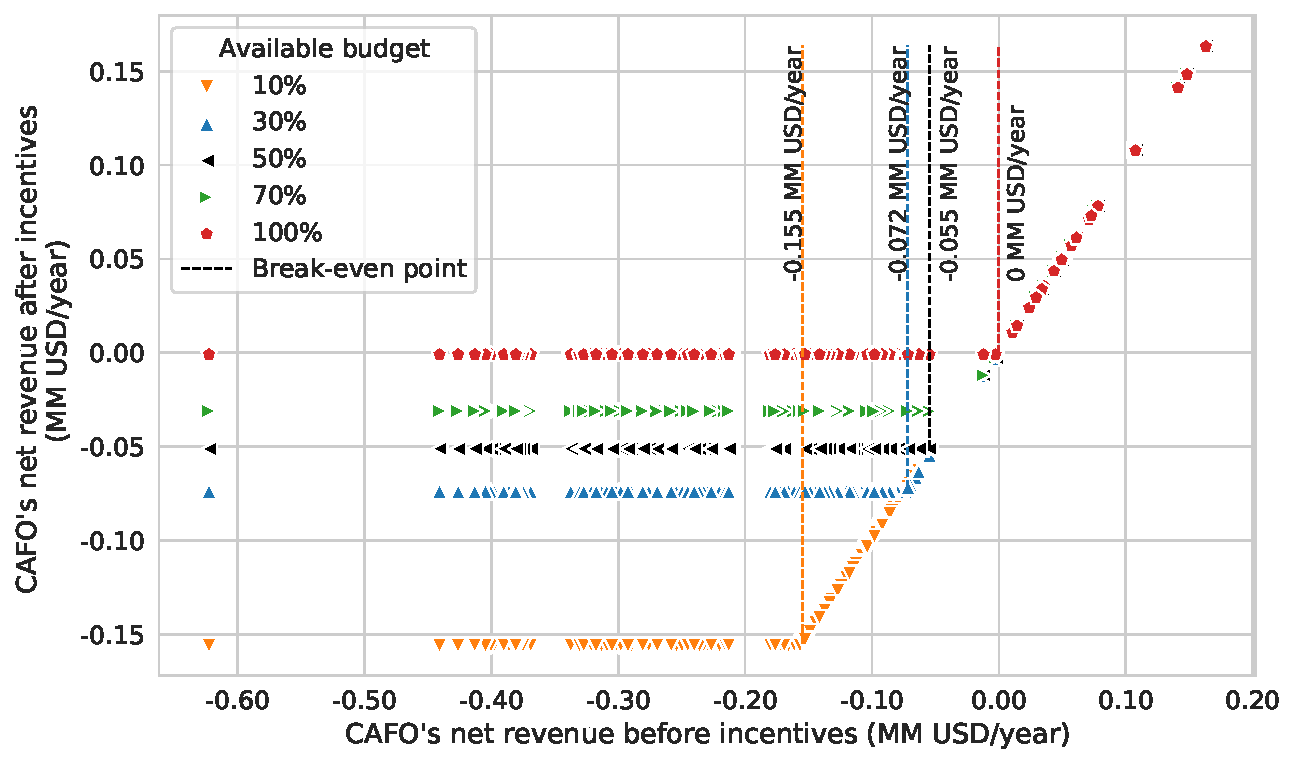
\includegraphics[width=\linewidth]{gfx/Chapter5/NashIncentv2.pdf}
		\caption{CAFOs net revenue after incentives allocation}
		\label{fig:NashRevenues}
	\end{subfigure}
	
	\caption{Distribution of incentives considering the Nash allocation scheme. Scenarios assuming available incentives equal to the 10\%, 30\%, 50\%, 70\%, and 100\% of the incentives needed to cover the economic losses of unprofitable P recovery systems in the Great Lakes area are illustrated.}
	\label{fig:AllNash}
\end{figure}

Figure \ref{fig:NashIncent} illustrates the distribution of incentives as a function of the net revenues of the P recovery system installed in each CAFO $c$ before any incentive is applied, Eq \ref{eq:NetRevBeforeInc}.

\begin{align}
& \text{Net revenue before incentives}_{c} \left(\frac{\text{USD}}{\text{year}}\right) = R_{c} - OPEX_{c} \label{eq:NetRevBeforeInc}
\end{align}

The cases where the available budget are the 10\%, 30\%, 50\%, 70\%, and 100\% of the incentives needed to cover the economic losses of unprofitable CAFOs are analyzed (22.3, 66.8, 111.3, 155.8 and 222.6 MM USD respectively). The last case is equivalent to the scenario studied above. It can be observed that the available incentives are allocated accordingly to the net revenues of each CAFO, promoting the allocation of larger incentives to the less profitable P recovery processes. Since the available incentives are limited, a break-even point determining the profitability level of the P recovery systems below which the incentives should be allocated is set for each scenario. As a result, the fewer incentives available, the more restrictive the break-even point is. Additionally, it can be observed that the displacement of the break-even points is progressively reduced as the available incentives increase, resulting in a marginal improvement between the scenarios considering the 50\% and 70\% of the economic resources needed to guarantee the economic neutrality of the nutrient management systems. In Figure \ref{fig:NashRevenues} we observe that, for each case evaluated, the allocation of limited incentives under the Nash scheme result in a uniform net revenue for those CAFOs receiving incentives. Additionally, we note that the economic looses have been mitigated in these facilities by the allocation of incentives. However, they are unable to be profitable due to the limited budget available. In addition, a correlation to estimate the fairness point as a function of available incentives has been developed based on these results, Eq. \ref{eq:FairnessPoint}.

\begin{align}
& \text{Break-even point}_c \ \ \ \left(\frac{\text{USD}}{\text{year}}\right) = -2.482\cdot10^{5} \cdot \left(0.955^{\left(R_{c} - OPEX_{c}\right)}\right) \label{eq:FairnessPoint}
\end{align}

\section{Conclusions}
The application of different incentives to promote the implementation of nutrient management systems at CAFOs is studied in this work, including the potential integration of phosphorus recovery technologies with the production of renewable electricity from biogas. 

The results reveal that the recovery of phosphorus is more economically feasible in the largest CAFOs due to the economies of scale. The deployment of phosphorus recovery processes is self-profitable through struvite sales only for the largest P recovery processes, which represent less than the 5 \% over the total CAFOs in all the studied states. However, the application of P credits increases the fraction of profitable processes around to 100\% in the states with large-size CAFOs (Michigan, Ohio and Wisconsin), and up to 80\% for the states with medium-size CAFOs (Indiana and Pennsylvania). The integration of phosphorus recovery technologies with anaerobic digestion and biogas upgrading processes does not result in any practical improvement in terms of economic performance unless incentives for phosphorus recovery are considered, since the revenues from electricity sales can not cover the investment and operating cost of these processes given current market values.

The total cost of phosphorus recovery, including the investment amortization, operating costs, and total cost of incentives is lower than the long-term economic losses due to phosphorus pollution for all the evaluated states and policies, proving that sustainable nutrient management systems are economically and environmentally beneficial. Correlations to estimate the incentives necessary for P recovery systems to achieve economic neutrality has been also proposed. Additionally, the fair distribution of limited incentives has been studied, determining the break-even point for the allocation of monetary resources based on the availability of incentives.

Future work is aimed at assessing the effect of biomethane production in the economy of the waste treatment systems, and the integration within a logistics network model for the developing of nutrient pollution and ecosystem integrated responses at regional spatial resolution.

\section*{Acknowledgments} \label{section:Acknowledgments}
\addcontentsline{toc}{section}{Acknowledgments}
This research was supported in part by an appointment for E.M.H. to the Research Participation Program for the Office of Research and Development, US EPA, administered by the Oak Ridge Institute for Science and Education through Interagency Agreement No. DW-89-92433001 between the US Department of Energy and the US Environmental Protection Agency. E.M.H. and M.M. acknowledge funding from Junta de Castilla y Le\'{o}n, Spain, under grant SA026G18 and grant EDU/556/2019. Y.H. and V.M.Z. acknowledge funding from the U.S. Department of Agriculture, National Institute of Food and Agriculture, under grant number 2017-67003-26055.

\textbf{Disclaimer:} The views expressed in this article are those of the authors and do not necessarily reflect the views or policies of the U.S. EPA. Mention of trade names, products, or services does not convey, and should not be interpreted as conveying, official U.S. EPA approval, endorsement, or recommendation.

\section*{Bibliography}
\addcontentsline{toc}{section}{Bibliography}

\printbibliography[heading=none]
\end{refsection}
\cleardoublepage
\part{Nitrogen management and recovery}\label{pt:Nitrogen}
%*****************************************
\chapter{Multi-scale techno-economic assessment of nitrogen recovery systems for swine operations }\label{ch:NitrogenTechs}
\chaptermark{Multi-scale techno-economic assessment of nitrogen recovery systems}
%*****************************************
\begin{refsection}[referencesCh6]
\section*{Abstract}
Intensive swine farming generates vast amounts of organic waste, which are an important source of nitrogen releases. Nitrogen released from farming activities contributes to multiple environmental problems, such as ecosystem fertilization, eutrophication of water systems, and greenhouse gases emissions. Nitrogen recovery is technically feasible, and there exists a number of processes for the processing of livestock waste recovering nitrogen in the form of different products.
In this work, a multi-scale techno-economic assessment of six systems for nitrogen recovery from swine waste, i.e., transmembrane  chemisorption, ammonia evaporation and scrubbing, striping in packed tower, MAPHEX, and struvite production, is performed. Additionally, the material flows from waste collection to final treatment are analyzed to determine the recovery efficiency and nitrogen losses for each  process. The results show that transmembrane chemisorption is the process with the lowest recovery cost, from 10.4 to 3.4 USD per kilogram of nitrogen recovered. Moreover, considering that economic losses due to the harmful effects of nitrogen into the environment are estimated at 32-35 USD per kilogram of nitrogen released, nitrogen recovery by processing swine waste through three technologies, i.e., transmembrane chemisorption, MAPHEX, and stripping in packed bed, reveals to be economically beneficial. This work estimates the cost of nitrogen recovery at swine operations, and it is intended to be a starting point for designing and evaluating regulations and incentives for the transition to a more sustainable paradigm for food production.

\bigskip
Keywords: Organic Waste; Nitrogen Recovery; Nutrient Pollution; Livestock Industry; Techno-economic assessment
\newpage

\section*{Resumen}
La cría intensiva de cerdos genera grandes cantidades de residuos orgánicos, que son una importante fuente de liberación de nitrógeno. El nitrógeno liberado por las actividades ganaderas contribuye a múltiples problemas medioambientales, como la fertilización de los ecosistemas, la eutrofización de los sistemas acuáticos y las emisiones de gases de efecto invernadero. La recuperación de nitrógeno es técnicamente factible, y existen varios procesos para el tratamiento de residuos ganaderos que recuperan el nitrógeno en forma de diferentes productos. En este trabajo se realiza una evaluación tecno-económica a escala múltiple de seis sistemas para la recuperación de nitrógeno a partir de residuos porcinos: quimisorción transmembrana, evaporación y lavado de amoníaco, stripping en lecho empaquetado, MAPHEX y producción de estruvita. Además, se analizan los flujos de material desde la recogida de residuos hasta el tratamiento final para determinar la eficiencia de recuperación y las pérdidas de nitrógeno de cada proceso. Los resultados muestran que la quimisorción transmembrana es el proceso con menor coste de recuperación, de 10,4 a 3,4 USD por kilogramo de nitrógeno recuperado. Además, teniendo en cuenta que las pérdidas económicas debidas a los efectos nocivos del nitrógeno en el medio ambiente se estiman en 32-35 USD por kilogramo de nitrógeno emitido, la recuperación de nitrógeno mediante el procesamiento de los residuos porcinos a través de tres tecnologías, quimisorción transmembrana, MAPHEX y stripping en lecho empaquetado, se revela económicamente beneficiosa. Este trabajo estima el coste de la recuperación de nitrógeno en las explotaciones porcinas y pretende ser un punto de partida para el diseño y la evaluación de normativas e incentivos para la transición a un paradigma más sostenible de la producción de alimentos.

\bigskip
Palabras clave: Residuos orgánicos; Recuperación de nitrógeno; Contaminación por nutrientes; Industria ganadera; Análisis tecnoeconómico
\newpage

\section{Introduction}
The agricultural sector has experimented an industrialization process since the XIX century, pursuing the intensification of the agri-products and food production, i.e., increasing the agricultural production per unit of input resources, including land, labor and feed among others \citep{FAOethics2004}. During the last decades, the agricultural intensification is driven by a sustained increase in the population, the average income growth in both developed and developing countries, and the trade liberalization and logistics advancements leading the transnational trade of products \citep{baker2014trends}. As a result of this intensification process, the largest quantity and variety of agri-products in the human history is produced and distributed nowadays. However, multiple environmental challenges must be faced as a consequence of the industrialization of the agriculture and farming activities: soil depletion of nutrients and organic matter as consequence of mono-cropping, excessive and inefficient use of synthetic fertilizers to maintain high cropping yields, spatial concentration and inappropriate management of livestock manure, biodiversity loss, etc. 
Focusing in the context of nutrient management, the use of synthetic fertilizers, and the detachment of arable lands and livestock facilities decoupled the previous link where the organic waste from livestock activities were used as nutrient and organic matter supply for crops \citep{bouwman2009human}. This decoupling has created a dependency on mineral (phosphorus) and synthetic (nitrogen) fertilizers, and the adequate management of animal manure has become a serious problem for concentrated animal feeding operations (CAFOs). Therefore, there is disconnection between localized areas with large concentrations of organic waste containing nutrients, such as the intensive livestock facilities, and croplands demanding nitrogen and phosphorus
%to keep high yield rates which relies
relying in synthetic and mineral fertilizers to keep high yield rates. Due to the sparse location of the facilities and the high density of organic wastes, including manure and digestate, the transportation of these wastes for nutrients redistribution is challenging and expensive \citep{sampat2018technologies}. Therefore, the implementation of technologies and processes for the recovery of nutrients in a form suitable for easy transport and use in croplands is of utmost importance, restoring the circularity of agricultural nutrients usage disrupted by industrial practices. However, the selection of the most suitable technology for an individual facility is not a trivial process, but involves multiple dimensions, including the recovery efficiency, the effect of the scale on the economic performance of the process, and the environmental footprint of the different technologies. Some previous works assessing and comparing technologies have been performed, but they do not capture the effect of the economies of scale \citep{munasinghe2020nitrogen, de2019resource}, or they are limited to a few number of technologies \citep{bolzonella2018nutrients}.
%, or they are not focused in livestock waste \citep{beckinghausen2020removal}. 
\citet{beckinghausen2020removal} reports a lack of techno-economic analyses for nitrogen recovery techniques to identify the most suitable process according to the characteristics of each facility. In addition, the previous studies do not capture the effects of integrating these processes with anaerobic digestion systems for energy recovery.

%In this work, a systematic techno-economic analysis, including the scale effect on the economic performance is carried out for comparing the state-of-the-art technologies for nitrogen recovery from livestock waste, {\color{red}{i.e., transmembrane  chemisorption, ammonia evaporation and scrubbing, striping in packed tower, aeration stripping, MAPHEX, and struvite production.}} A material flow analysis (MFA) from waste collection to final treatment is combined with the are analyzed
In this work, six state-of-the-art technologies for nitrogen recovery from livestock waste, i.e., transmembrane  chemisorption, ammonia evaporation and scrubbing, striping in packed tower, MAPHEX, and struvite production, are systematically assessed and compared. Each system is evaluated performing a material flow analysis (MFA) of the whole process, from waste collection to the final treatment, and a techno-economic analysis (TEA) capturing the effect of the economies of scale on the cost of nitrogen recovery.
%through the development models for the calculation of the energy and mass balances, including the recovery yield; and for economic evaluation purposes. 
The objective is to determine the most adequate technologies to close the nutrients loop from livestock to crops, and the optimal conditions for the implementation of
%each one of
these systems. The processes for livestock waste treatment studied involve all stages from waste collection to the production of the nutrient-rich final product: manure preconditioning, optional biogas production valorization, solid-liquid separation of manure or digestate, and nutrients recovery. The assessment of such technologies is performed through detailed mathematical models of the processes based on first principles and experimental data, resulting in a flexible framework able to analyze different combinations and scales of technologies for the treatment of swine waste. The information obtained from the techno-economic assessment of nitrogen recovery technologies is key for the further development of policies to promote nutrient recovery and to mitigate the environmental footprint of swine farming activities.
%with special emphasis on the resiliency of the technology selected for each scenario, since there exist multiple variable factors that affect the performance of nutrient recovery facilities, e.g., the variability of waste composition, the prices of the products obtained, and the cost of the utilities required by each unit. Therefore, a flexible framework capable of assessing changes in input parameters is developed, allowing the study of the impact of the fluctuation of these variables on the results obtained, including the technical and economic performance of the different nutrient recovery technologies, and the selection of the optimal system. In addition, the application of potential government incentives is evaluated, determining the most cost-effective incentive policies to mitigate the economic impact of the nitrogen recovery facilities on the economies of the livestock facilities.  

\section{Methods}
\subsection{Livestock waste}
Swine manure generated by animals at different life stages have different composition, as well as a different waste generation ratio, i.e., waste mass generated per animal per day. Data reported by the US Department of Agriculture \citep{USDAWaste, Kellog2000} is used to determine the waste flow and composition as a function of the number of animals in a facility and their type, as listed in Table \ref{table:SwineWaste}. AU denotes animal units, which is defined as 1000 pounds (453.6 kg) of live animal \citep{animal_unit_definition}.

%\begin{table}[h] 
	%%	\begin{adjustwidth}{}{}
		%		\centering
		%		\caption{Swine waste characterization. Adapted from \protect\citet{USDAWaste, Kellog2000}.} \label{table:SwineWaste}
		%		\resizebox{\columnwidth}{!}{
			%		\begin{threeparttable}
				%		\begin{tabular}{@{}ccccccc@{}}
					%		\toprule
					%		Components        & Units     & Sow Gestating & Sow Lactating & Boar & Piglets Nursery & Piglets Grow\\to Finish \\ \midrule
					%		Animals:AU      & ratio     & 2.67          & 2.67          & 2.67 & 9.09            & 9.09                   \\
					%		Weight            & $\sfrac{\text{lb}}{\text{d AU}}$ & 25            & 59            & 19   & 88              & 65                     \\
					%		Volume            & $\sfrac{\text{ft\textsuperscript{3}}}{\text{d AU}}$ & 0.41          & 0.97          & 0.3  & 1.4             & 1.1                    \\
					%		Moisture          & \%wt  & 90            & 90            & 90   & 90              & 90                     \\
					%		TS                & $\sfrac{\text{lb}}{\text{d AU}}$ & 2.5           & 5.9           & 1.9  & 10              & 6.5                    \\
					%		VS                & $\sfrac{\text{lb}}{\text{d AU}}$ & 2.3           & 5.4           & 1.7  & 8.8             & 5.4                    \\
					%		N                 & $\sfrac{\text{lb}}{\text{d AU}}$ & 0.16          & 0.45          & 0.14 & 0.92            & 0.54                   \\
					%		P                 & $\sfrac{\text{lb}}{\text{d AU}}$ & 0.05          & 0.13          & 0.05 & 0.15            & 0.09                   \\
					%		K                 & $\sfrac{\text{lb}}{\text{d AU}}$ & 0.11          & 0.28          & 0.09 & 0.35            & 0.24                   \\
					%		N\textsubscript{inorganic}:N\textsubscript{total} & ratio     & 0.61          & 0.61          & 0.61 & 0.61            & 0.61                   \\
					%		N\textsubscript{organic}:N\textsubscript{total}   & ratio     & 0.39          & 0.39          & 0.39 & 0.39            & 0.39                   \\
					%		P\textsubscript{inorganic}:P\textsubscript{total} & ratio     & 0.58          & 0.58          & 0.58 & 0.58            & 0.58                   \\
					%		P\textsubscript{organic}:P\textsubscript{total}   & ratio     & 0.42          & 0.42          & 0.42 & 0.42            & 0.42                   \\ \bottomrule
					%	\end{tabular}
				%		\begin{tablenotes}
					%		\item AU: Animal units.
					%		\item TS: Total solids.
					%		\item VS: Volatile solids.
					%		\item N: Nitrogen.
					%		\item P: Phosphorus.
					%		\item K: Potassium.
					%	\end{tablenotes}
				%	\end{threeparttable}
			%	}
		%\end{table}
	
\begin{table}[h] 
%	\begin{adjustwidth}{}{}
	\centering
	\caption{Swine waste characterization. Adapted from \protect\citet{USDAWaste, Kellog2000}.} \label{table:SwineWaste}
	\resizebox{\columnwidth}{!}{
		\begin{threeparttable}
			\begin{tabular}{@{}ccccccc@{}}
				\toprule
				Components        & Units     & Sow Gestating & Sow Lactating & Boar & Piglets Nursery & Piglets Grow\\to Finish \\ \midrule
				Animals:AU      & ratio     & 2.67          & 2.67          & 2.67 & 9.09            & 9.09                   \\
				Weight            & $\sfrac{\text{kg}}{\text{d AU}}$ & 11.34            & 26.76            & 8.62   & 39.92              & 29.48                     \\
				Volume            & $\sfrac{\text{m\textsuperscript{3}}}{\text{d AU}}$ & 0.012          & 0.027          & 0.0085  & 0.040            & 0.031                    \\
				Moisture          & \%wt  & 90            & 90            & 90   & 90              & 90                     \\
				TS                & $\sfrac{\text{kg}}{\text{d AU}}$ & 1.13           & 2.68           & 0.86  & 4.54              & 2.95                    \\
				VS                & $\sfrac{\text{kg}}{\text{d AU}}$ & 1.04           & 2.45           & 0.77  & 3.99             & 2.45                    \\
				N                 & $\sfrac{\text{kg}}{\text{d AU}}$ & 0.073          & 0.20          & 0.064 & 0.42            & 0.24                   \\
				P                 & $\sfrac{\text{kg}}{\text{d AU}}$ & 0.023          & 0.059          & 0.023 & 0.068            & 0.041                   \\
				K                 & $\sfrac{\text{kg}}{\text{d AU}}$ & 0.050          & 0.13          & 0.041 & 0.16            & 0.11                   \\
				N\textsubscript{inorganic}:N\textsubscript{total} & ratio     & 0.61          & 0.61          & 0.61 & 0.61            & 0.61                   \\
				N\textsubscript{organic}:N\textsubscript{total}   & ratio     & 0.39          & 0.39          & 0.39 & 0.39            & 0.39                   \\
				P\textsubscript{inorganic}:P\textsubscript{total} & ratio     & 0.58          & 0.58          & 0.58 & 0.58            & 0.58                   \\
				P\textsubscript{organic}:P\textsubscript{total}   & ratio     & 0.42          & 0.42          & 0.42 & 0.42            & 0.42                   \\ \bottomrule
			\end{tabular}
			\begin{tablenotes}
				\item AU: Animal units.
				\item TS: Total solids.
				\item VS: Volatile solids.
				\item N: Nitrogen.
				\item P: Phosphorus.
				\item K: Potassium.
			\end{tablenotes}
		\end{threeparttable}
	}
\end{table}

\subsection{Nitrogen management systems assessment framework} \label{section:NitrogenManagModels}
Swine manure processing involves several stages from manure collection to resources recovery, as shown in Figure \ref{fig:techs_diagrams}. In this section the modeling details of each stage are drawn.
\begin{figure}[h]
	\centering
	%	\begin{subfigure}[t]{0.5\linewidth}
		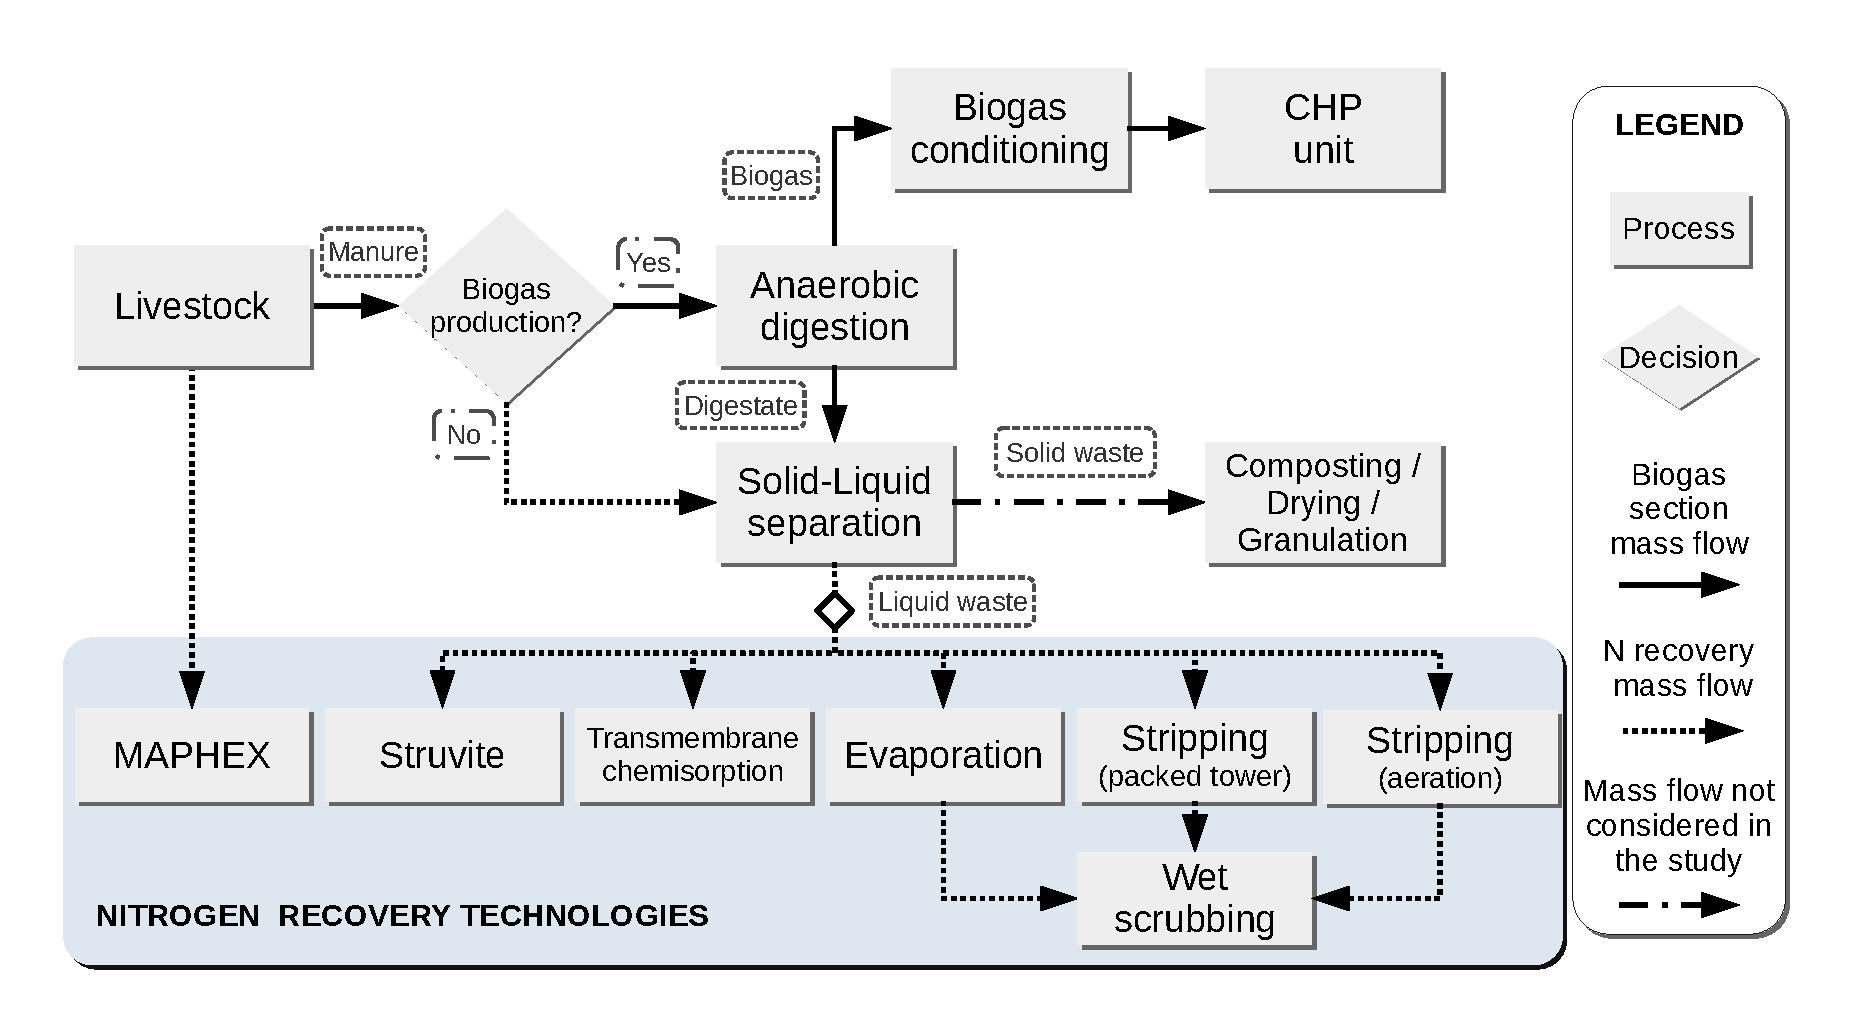
\includegraphics[width=0.75\linewidth, trim={1cm 1cm 1cm 1cm},clip]{gfx/Chapter6/Process_Flowsheet2.pdf} 
		\caption{Flowchart of the processes assessed for the processing of livestock waste}
		\label{fig:techs_diagrams}
	\end{figure}

\subsubsection{Anaerobic digestion}
Swine manure can be processed in an anaerobic digestion (AD) unit for the production of biogas and digestate. These materials can be further processed to recover valuable resources, such as electricity and thermal energy from biogas, and nutrients from digestate. As a result of the digestion process, the organic and inorganic fractions of nutrients (i.e., nitrogen and phosphorus) vary due to the partial mineralization of the organic fraction of nitrogen and phosphorus. Therefore, the amount of inorganic nutrients in the digestate is larger than in raw manure, as shown in Table \ref{table:ADWaste} \citep{fangueiro2020available}. In addition, the amount of total solids decreases as a consequence of the transformation of volatile solids into biogas. AD process is typically carried out either at mesophilic (25 and 45 \textdegree C) and thermophilic (45 and 50 \textdegree C) temperatures and atmospheric pressure, with retention times between 30-40 and 15-20 days respectively. There also exist low temperature digestion at psychrophilic conditions ($<$ 25 \textdegree C), although it involves longer retention times between 70 and 80 days. The higher the temperature, the shorter the retention time \citep{Seadi2008}. A digestion temperature  of 40 \textdegree C and a retention time $\left( {HRT}_{\text{AD}} \right) $ of 21 days have been assumed in this work \citep{bolzonella2018nutrients}. 
%In Table ?? the variations in the organic and inorganic fractions of nutrients are 

\begin{table}[h] 
	\centering
	\caption{Variation of the inorganic fraction of nutrients biogas generation after anaerobic digestion of swine waste. Adapted from \protect\citet{fangueiro2020available}.} \label{table:ADWaste}
	\begin{threeparttable}
		\begin{tabular}{@{}cc@{}}
			\toprule
			Parameter      & Variation (\%) \\ \midrule
			TS             & -45            \\
			VS             & -52.5          \\
			N\textsubscript{inorganic}         & 45             \\
			P\textsubscript{inorganic}         & 16             \\
			%		$\sfrac{\text{m}^3_{\text{biogas}}}{\text{kg}_{\text{VS}}}$ & 0.57           \\
			\bottomrule
		\end{tabular}
		\begin{tablenotes}
			\item TS: Total solids.
			\item VS: Volatile solids.
			\item N: Nitrogen.
			\item P: Phosphorus
			.
		\end{tablenotes}
	\end{threeparttable}
\end{table}

The composition of biogas produced is based on data reported by \citet{Ciborowski}. The energy requirements of the AD unit $\left( Q_{\text{digester}} \right)$, described in Eq  \ref{eq:general1Manuscript}, comprise the energy required for substrate warming up from ambient temperature (assumed to be 12 \textdegree C) $\left( Q_{\text{waste}} \right)$ to the digestion temperature (40 \textdegree C),
%Eq. , 
and the energy supplied to offset the digester heat losses $\left( Q_{\text{losses}} \right)$.
%, {\color{blue}{Eq. \ref{eq:Qwaste} and \ref{eq:Qlooses} of the Supplementary Material}} respectively. The global heat transfer coefficients ($U$) for the different digester surfaces are collected in Table \ref{table:AD_U}. The area of different surfaces is estimated through preliminar equipment design, Eqs. \ref{eq:Vdigester1} to \ref{eq:Aroof}, assuming a maximum digester of 6000 m\textsuperscript{3} \citep{6000AD}. The installation of multiple digestion units is considered if the waste flow exceed this capacity.
{\color{blue}{The details of the energy balance to the AD unit can be found in the Supplementary Material, Eqs. \ref{eq:general1} to \ref{eq:Aroof}.}} A maximum digester size $\left( n_{\text{AD, }max} \right)$ of 6000 m\textsuperscript{3} is assumed \citep{ADSize}.

\begin{align}
	& Q_{\text{digester}} = Q_{\text{waste}} + Q_{\text{losses}} \label{eq:general1Manuscript}
	%	\\
	%	& Q_{\text{waste}} = \dot{m}_{\text{waste}} \cdot c_{p} \cdot \left(T_{\text{digestion}} - T_{\text{ambient}}\right) \label{eq:Qwaste} \\
	%	& Q_{\text{losses}} = \sum_{i} U_{i} A_{i} \left(T_{\text{digestion}} - T_{\text{ambient}}\right)\label{eq:Qlooses}, \forall i  \in \{\text{roof, walls, floor}\}
\end{align}

%\begin{table}[h] 
	%	\centering
	%	\caption{Anaerobic digester design parameters. \protect\citep{ADPennState}.} \label{table:AD_U}
	%	%	\begin{threeparttable}
		%	\begin{tabular}{@{}ccc@{}}
			%		\toprule
			%		\multicolumn{1}{c}{Parameter} & Unit  & \multicolumn{1}{c}{Value} \\ \midrule
			%		$U_{\text{floor}}$                        & $\sfrac{\text{W}}{\text{m}^2 \text{ K}}$     & 2.85                      \\
			%		$U_{\text{wall}}$                         & $\sfrac{\text{W}}{\text{m}^2 \text{ K}}$     & 0.39                      \\
			%		$U_{\text{roof}}$                         & $\sfrac{\text{W}}{\text{m}^2 \text{ K}}$     & 0.3                       \\
			%		$V_{\text{max}}$                         & m$^3$    & 6000                      \\
			%		$V_{\text{freeboard}}$                   & \%    & 30                        \\
			%		$HRT$                           & days  & 21                        \\
			%		$D_{\text{digester}}$:$H_{\text{digester}}$                           & ratio & 1.1                       \\
			%		$A_{\text{roof}}$:$A_{\text{floor}}$                  & ratio & 1.62                      \\ \bottomrule
			%	\end{tabular} 
		%	%		\begin{tablenotes}
			%	%			\item TS: Total solids.
			%	%			\item VS: Volatile solids.
			%	%		\end{tablenotes}
		%	%	\end{threeparttable}
	%\end{table}
%
%\begin{align}
	%	& V_{\text{digester}} = \frac{\dot{m}_{\text{waste}}}{\rho_{\text{waste}}} \cdot HRT \cdot \left(1 + \frac{V_{\text{freeboard}}}{100}\right) \label{eq:Vdigester1}\\
	%	& V_{\text{digester}} = A_{\text{floor}} \cdot \frac{D_{\text{digester}}}{D_{\text{digester}}:H_{\text{digester}}} \label{eq:Vdigester2} \\
	%	& A_{\text{floor}} = \pi \cdot \frac{D_{\text{digester}}^2}{4} \label{eq:Afloor} \\
	%	& A_{\text{wall}} = 2 \pi \cdot \frac{D_{\text{digester}}}{2} \cdot \frac{D_{\text{digester}}}{D_{\text{digester}}:H_{\text{digester}}} \label{eq:Awall}\\
	%	& A_{\text{roof}} = A_{\text{floor}} \cdot \left(A_{\text{roof}}:A_{\text{floor}}\right) \label{eq:Aroof}
	%\end{align}

%As shown in Figure \ref{fig:AD_size_2cost}, 
Correlations for capital expenditures (CAPEX) and operating expenses (OPEX) estimation as a function of animal units have been developed based on data reported by the USDA \citep{USDAOM}, as shown in Eqs. \ref{eq:nAD}-\ref{eq:OM_costs} and Figure \ref{fig:AD_size_2cost} of the Supplementary Material, where $\dot{m}_{digestate}$ denotes the digestate flow and $AU$ the number of animal units. It should be noted that operating and management (O\&M) cost does not include the capital cost amortization.
%\begin{figure}[H]
%	\centering
%	%	\begin{subfigure}[t]{0.5\linewidth}
	%	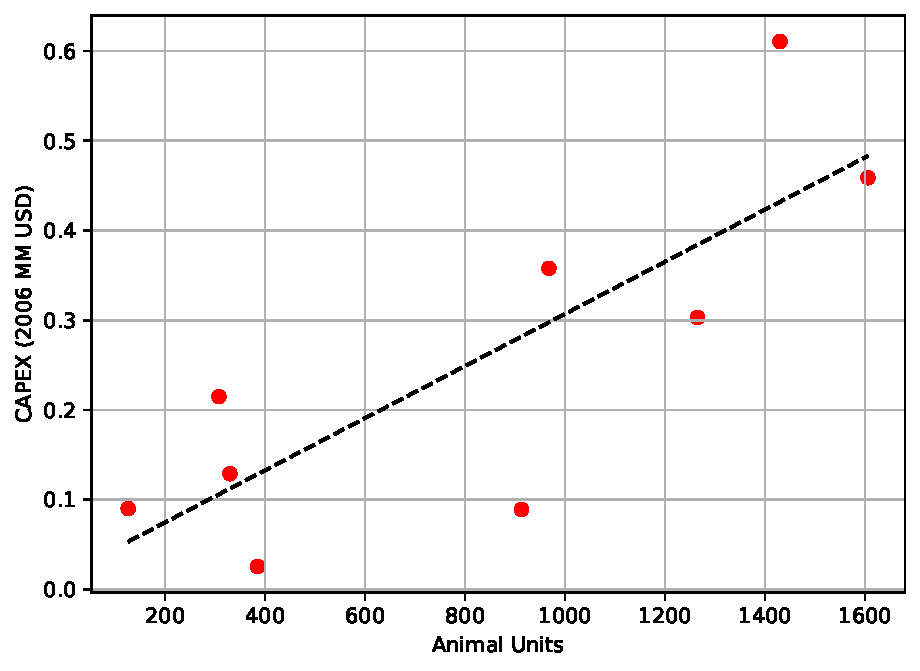
\includegraphics[width=0.6\linewidth, trim={0cm 0cm 0cm 0cm},clip]{AD_SizeCost_Swine.pdf} 
	%	\caption{Flowchart of the processes assessed for the processing of livestock waste}
	%	\label{fig:AD_SizeCost_Swine}
	%\end{figure}

%\begin{figure}[H]
	%	\centering
	%	\begin{subfigure}[t]{0.48\textwidth}
		%		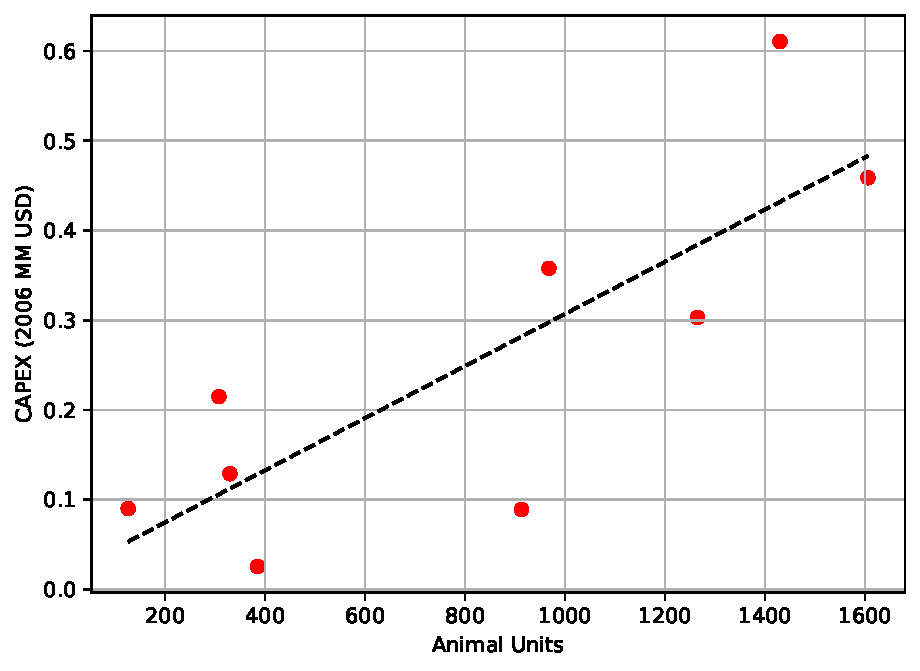
\includegraphics[width=\textwidth, trim={0cm 0cm 0cm 0cm},clip]{AD_SizeCost_Swine.pdf}
		%		\caption{Cost of AD units as a function of animal units.}
		%		\label{fig:AD_SizeCost_Swine}
		%	\end{subfigure}
	%	\quad
	%	\begin{subfigure}[t]{0.47\textwidth}
		%		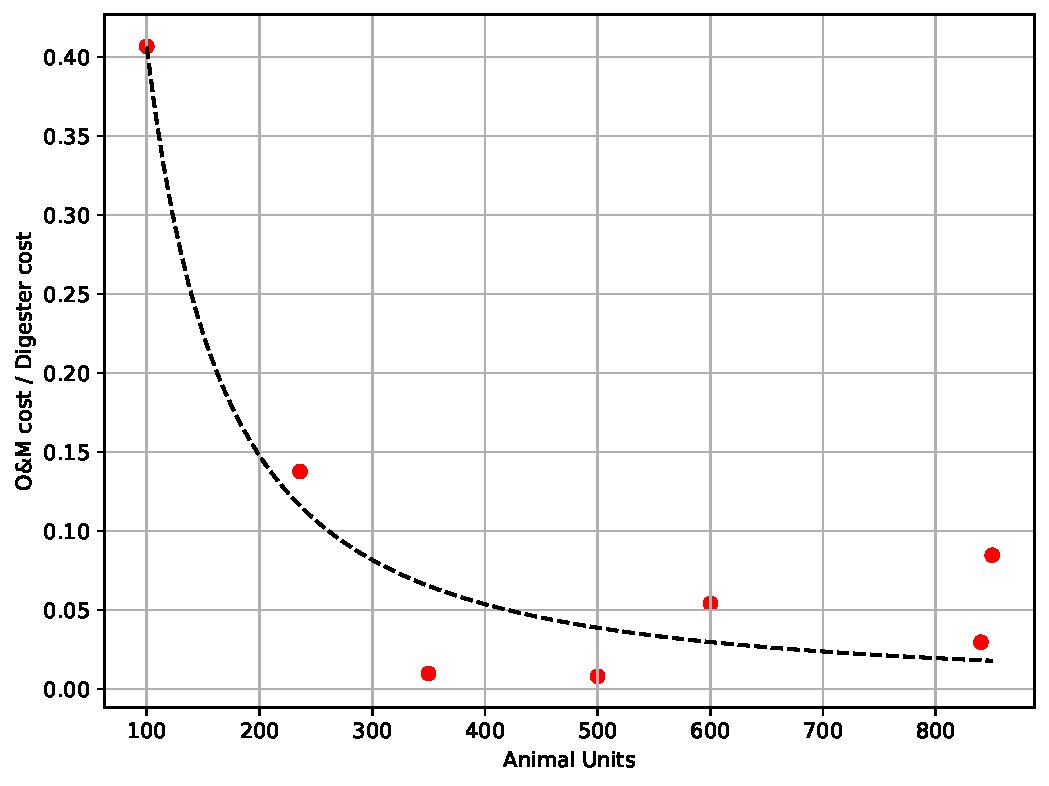
\includegraphics[width=\textwidth]{AD_size_OM_Unit_cost.pdf} 
		%		\caption{O\&M costs as a function of animal units.}
		%		\label{fig:AD_size_OM_Unit_cost}
		%	\end{subfigure}
	%	
	%	\caption{Correlations between AD capital and O\&M costs, and the number of cattle in the livestock facility. Data from \protect\citet{USDA_OM}.}
	%	\label{fig:AD_size_2cost}
	%\end{figure}

\begin{align} 
	& n_{\text{AD}} = \ceil*{\frac{\dot{m}_{digestate} \cdot HRT_{\text{AD}}}{n_{\text{AD, }max}}} \label{eq:nAD} \\
	& \text{CAPEX (MM USD (2019))} = \left(2.9069 \cdot 10^{-4} \cdot AU+0.01625\right) \cdot 1.216 \label{eq:inv_costs}\\ \nonumber\\
	%	& \frac{\text{O\&M}} {\text{Installation cost}} \text{ ratio} = \frac{15858.710}{(1+\left(N_{animals} \cdot 13.917\right)^{1.461}} \label{eq:OM_costs}\\ \nonumber\\
	& \text{OPEX } \left(\frac{\text{MM USD (2019)}}{\text{year}}\right) = \left(\frac{15.858\cdot 10^{3}}{1+\left(AU \cdot 13.917\right)^{1.461}}\right) \cdot \text{CAPEX} \label{eq:OM_costs}
	%	& \frac{\text{O\&M}} {\text{CAPEX}} \text{ ratio} = \frac{15.858\cdot 10^{3}}{(1+\left(AU \cdot 13.917\right)^{1.461}} \label{eq:OM_costs}\\ \nonumber\\
	%	& \text{OPEX } = \text{O\&M costs} + \frac{\text{Investment cost}}{\text{Plant lifetime}} \label{eq:OM_inv_costs}
\end{align}

\subsubsection{Biogas conditioning}
The raw biogas generated is conditioned to remove
%the main harmful elements within it. 
its impurities. Most of moisture is removed through condensation by compressing and cooling down the biogas stream. H\textsubscript{2}S is removed by using a fixed bed of Fe\textsubscript{2}O\textsubscript{3}, capturing the hydrogen sulfur
%in the form of 
as Fe\textsubscript{2}S\textsubscript{3}. The bed can be regenerated using the oxygen contained in air, leading to the formation of elementary sulfur \citep{ryckebosch2011techniques}. Ammonia and remaining moisture are removed through a pressure swing adsorption (PSA) system. For both processes, two adsorption units are typically installed in-parallel arrangement, so that one unit is in operation while the other bed is undergoing regeneration. Removal yields of 100\% have been assumed. More details can be found in {\color{blue}{Section \ref{section:BiogasConditioningNRecovery} of the Supplementary Material.}}

\subsubsection{Combined heat and power generation}
Biogas is valorized using a combined heat and power (CHP) unit to produce electricity and heat, which can be used to cover the thermal energy demand of the AD unit, and also for the nitrogen recovery processes if a source of heat is needed, e.g., ammonia evaporation. The energy recovered from biogas is estimated through its low heating value (LHV). LHV of biogas is a function of methane content, and it can be estimated using Eq. \ref{eq:LHV} \citep{BiogasLHV}, where $x_{\text{CH4}}$ refers to the methane mass fraction. Biogas combustion in the CHP unit is performed considering a 20\% air excess.

\begin{align}
	& LHV_{\text{biogas}} \left(\sfrac{\text{J}}{\text{m}^3}\right)= -46.26 \cdot 10^6 \cdot x_{\text{CH4}}^2 + 70.87 \cdot 10^6 \cdot x_{\text{CH4}} + 2.29\cdot 10^6 \label{eq:LHV}
\end{align}

Based on data reported by manufacturers, the electricity and thermal efficiencies assumed are 40\% and 50\% respectively \citep{ClarkeEnergy}. The heat produced can be classified in high grade heat (HGH), which is recovered from the exhaust gases of combustion at 450 \textdegree C, and low grade heat (LGH) recovered from other points of the equipment at lower temperature. HGH and LGH account for 62\% and 38\% of total heat energy respectively.
%such as the lubrication oil and jacket water of the engine. 
LGH is used to cover the energy demand of AD units, while HGH is used for heat-intensive processes such as ammonia evaporation. If LGH from the CHP unit is not enough to cover the energy requirements of AD process, a fraction of HGH can be used to supplement the thermal energy supply. 

\subsubsection{Digestate solid-liquid separation}
Nutrients contained in manure or digestate form organic and inorganic compounds. On the one hand, organic nutrients are in the form of carbon-based solid compounds, and therefore are mostly contained in the solid phase of waste. The nutrients bonded to organic compounds are not available for plants immediately, but they have to undergo a mineralization process to be transformed into inorganic nutrients \citep{USDAWaste}. On the other hand, inorganic nutrients are those forming inorganic compounds. Since they are water soluble, inorganic nutrients are mostly present in the liquid phase of waste. 
%Inorganic nutrients can be taken by plants in plants, including algae involved in HABs. 

The inorganic fraction of nutrients is recovered through a solid-liquid separation stage. The liquid fraction, containing most of inorganic nutrients, will be further processed for nutrient recovery. The solid phase of waste can be composted, promoting the mineralization of a fraction of the organic nutrients. The compost obtained can be used as a nutrient supplementation for crops. A screw press unit is considered for waste liquid-solid phases separation in this study \citep{MollerSL}. The partition coefficients for the different components, CAPEX estimation, and electricity consumption considering the discretization of equipment size due to the commercial sizes available, are shown in the {\color{blue}{ Section \ref{section:SLSeparationNRecovery} of the Supplementary Material.}}
%Table 6S of 
%the Supplementary Material. 
%Assuming the discretization of units due to the commercial sizes available, the investment and operating costs for the screw press equipment are presented in 
%Figure 9S of 
%the Supplementary Material.

\subsubsection{Nitrogen recovery systems}
The technologies for nitrogen recovery assessed in this work, illustrated in Figure \ref{fig:NRcoveryTechsDiagrams}, are described in this section, as well as their main modeling details.
%for performing a techno-economic assessment of these processes. 
%We note that, although the aim of this work is to evaluate the recovery of nitrogen, some of these processes recover both nitrogen and phosphorus. Phosphorus recovery efficiency of these processes is reported for a more detailed description and modeling.

\begin{sidewaysfigure}
%\begin{figure}
\begin{subfigure}{.5\textwidth}
	\centering
	\includegraphics[width=0.45\linewidth, trim={1cm 7.5cm 1cm 7cm},clip]{gfx/Chapter6/MULTIFORM.pdf} 
	\caption{Scheme of MULTIFORM process.}
	\label{fig:MULTIFORMscheme}
\end{subfigure}%
\begin{subfigure}{.5\textwidth}
	\centering
	%	\begin{subfigure}[t]{0.5\linewidth}
	\includegraphics[width=0.5\linewidth, trim={1cm 1cm 1cm 1cm},clip]{gfx/Chapter6/MAPHEX.pdf} 
	\caption{Scheme of MAPHEX process.}
	\label{fig:MAPHEXscheme}
\end{subfigure}
\\
\vspace{0.5cm}
\begin{subfigure}{.5\textwidth}
	\centering
	%	\begin{subfigure}[t]{0.5\linewidth}
	\includegraphics[width=0.8\linewidth, trim={1cm 1cm 1cm 1cm},clip]{gfx/Chapter6/Membrane2.pdf} 
	\caption{Diagram of a membrane module.}
	\label{fig:membrane_diagrams}
\end{subfigure}%
\begin{subfigure}{.5\textwidth}
	\centering
	%	\begin{subfigure}[t]{0.5\linewidth}
	\includegraphics[width=0.7\linewidth, trim={0cm 0cm 0cm 0cm},clip]{gfx/Chapter6/BeltDryerFinal3.pdf} 
	\caption{Belt dryer scheme.}
	\label{fig:BeltDryerScheme}
\end{subfigure}
\\
\centering
\begin{subfigure}{.4\textwidth}
\vspace{0.5cm}
\centering
%	\begin{subfigure}[t]{0.5\linewidth}
	\includegraphics[width=0.75\linewidth, trim={0cm 0cm 0cm 0cm},clip]{gfx/Chapter6/StrippingScrubbing.pdf} 
	\caption{Stripping and scrubber towers scheme.}
	\label{fig:ScrubberScheme}
\end{subfigure}
\caption{Nitrogen recovery systems assessed in the techno-economic assessment.}
\label{fig:NRcoveryTechsDiagrams}
%\end{figure}
\end{sidewaysfigure}

%\paragraph{\textbf{Struvite production: Multiform system}}
%{\color{blue}{Adapt text to nitrogen recovery}}

%Nitrogen can be recovered in the form of struvite.
\textbf{Struvite production (Multiform system):} Struvite is a mineral comprised by magnesium, ammonium, and phosphate that can be formed from different  organic wastes by the chemical reaction shown in Eq. \ref{eq:struvite}. The formation of struvite is a process that can be used for ammonia and phosphorus recovery by precipitation \citep{martin2020m}. MgCl\textsubscript{2} is supplied to the reactor at a phosphorus to magnesium molar ratio of 2 to increase struvite supersaturation \citep{bhuiyan2008phosphorus}. However, since phosphorus concentration in manure is lower than nitrogen concentration, phosphorus acts as the limiting reactant for struvite formation, and in turn, for nitrogen recovery. In this study, pH is adjusted to 9 for optimal struvite formation using sodium hydroxide \citep{Tao}.

\begin{align}
	& \text{MgNH}_{4}\text{PO}_{4} \cdot 6\text{H}_{2}\text{O} \downarrow \ \xrightleftharpoons[]{} \text{Mg}^{2+} + \text{NH}_{4}^{+} + \text{PO}_{4}^{3-} \label{eq:struvite}
\end{align}

Ammonium, phosphate, and other relevant compounds for struvite formation, such as carbonates competing for phosphate ions to form calcium-based precipitates, are part of chemical systems controlled by thermodynamic equilibrium. Therefore, a thermodynamic model for the formation of struvite and calcium precipitates accounting the variability of elements concentration in manure has been developed in a previous work \citep{martin2020m}.
The chemical systems considered in the model for estimating struvite formation are included {\color{blue}{in Tables 1S and 2S of the Supplementary Material.}}
Particularly, we note that calcium ions compete with magnesium ions for the phosphate ions, hindrancing the formation of struvite. Therefore, a correlation
%developed in a previous work has been used to compute
to estimate the formation of struvite through the fraction of phosphorus recovered as struvite $\left(x_{\text{struvite} \left(\text{PO}_{4}^{3-}\right) }\right) $ as a function of calcium concentration in the waste has been used in this work, Eq. \ref{eq:sigmoidal_Ca_StrYieldManuscript} \citep{martin2020m}. $x_{\text{Ca}^{2+}:\text{PO}_{4}^{3-}}$ denotes the molar calcium-phosphate ratio, while $\dot{m}_{i}$ and $MW_i$ refer to the mass flow and molecular weight of the component $i$ respectively. We note that this correlation is valid for estimating struvite formation at a pH of 9.
% \ref{table:pK}, as well as the thermodynamic equilibrium constant of each equilibrium ($p_K$).
Based on this correlation,
%the correlation shown in Eq. \ref{eq:sigmoidal_Ca_StrYield}, 
the amount of nitrogen recovered is estimated through Eq. \ref{eq:N_MultiformManuscript}.
% More details about the model developed for struvite and calcium precipitates formation are reported in \citet{martin2020m}.

\begin{align}
	& x_{\text{struvite} \left(\text{PO}_{4}^{3-}\right) }= \frac{0.798}{1+\left(x_{\text{Ca}^{2+}:\text{PO}_{4}^{3-}} \cdot 0.576\right)^{2.113}} \label{eq:sigmoidal_Ca_StrYieldManuscript}
	\\
	& \dot{m}_{\text{struvite } recovered} = \dot{m}_{\text{P } in}  \cdot x_{\text{struvite} \left(\text{PO}_{4}^{3-}\right) } \cdot \frac{MW_{\text{struvite}}}{MW_{\text{P}}} \label{eq:Struvite_MultiformManuscript}
	\\
	& \dot{m}_{\text{N } recovered} =  \dot{m}_{\text{struvite } recovered} \cdot \frac{MW_{\text{N}}}{MW_{\text{struvite}}} \label{eq:N_MultiformManuscript}
	%\\ 
	%& \dot{m}_{\text{N } released} = \dot{m}_{\text{N } in} - \dot{m}_{\text{struvite } recovered} \cdot \frac{MW_{\text{N}}}{MW_{\text{struvite}}}
\end{align} 

%\begin{table}[H] 
	%	\begin{adjustwidth}{}{}
		%		\centering
		%		\caption{Chemical equilibrium considered for predicting struvite formation.} \label{table:pK}
		%		\begin{tabular}{c c c c}
			%			\toprule
			%			Name	& Chemical system &${pK}$	&Source	\\ \midrule
			%			Ammonia & $\text{NH}_{4}^{+} \leftrightarrow \text{NH}_{3} + \text{H}^{+}$	&9.2 &\citep{Bates}	\\ 
			%			Water & $\text{H}_{2}\text{O} \leftrightarrow \text{OH}^{-} + \text{H}^{+}$	&14  &\citep{Skoog}	\\ 
			%			\multirow{3}{*}{Phosphoric acid} & $\text{H}_{3}\text{PO}_{4} \leftrightarrow \text{H}_{2}\text{PO}_{4}^{-} + \text{H}^{+}$	&2.1	&\citep{Ohlinger}	\\ 
			%			&$\text{H}_{2}\text{PO}_{4}^{-} \leftrightarrow \text{HPO}_{4}^{2-} + \text{H}^{+}$	&7.2  &\citep{Ohlinger}	\\ 
			%			&$\text{HPO}_{4}^{2-} \leftrightarrow \text{PO}_{4}^{3-} + \text{H}^{+}$	&12.35 &\citep{Ohlinger}	\\ 
			%			\multirow{2}{*}{Carbonic acid} & $\text{H}_{2}\text{CO}_{3} \leftrightarrow \text{HCO}_{3}^{-} + \text{H}^{+}$	&6.35	&\citep{Skoog}	\\  
			%			&$\text{HCO}_{3}^{-} \leftrightarrow \text{CO}_{3}^{2-} + \text{H}^{+}$	&10.33	&\citep{Skoog}	\\ \bottomrule
			%		\end{tabular}
		%	\end{adjustwidth}
	%\end{table}

Multiform Harvest is a commercial-level technology selected for the production of struvite from swine waste, since a previous work \citep{martin2021geospatial} found this system as the most cost-effective struvite production process in a wide range of capacities for waste processing.
%This , shown in Fig. \ref{fig:MULTIFORMscheme}, is a commercial
This technology is based on a single pass fluidized bed reactor (FBR), with no recirculation, and conical design, as shown in Fig. \ref{fig:MULTIFORMscheme}. The organic waste is pumped to the bottom of the reactor, as well as the magnesium supplement. The struvite particles grow, increasing their size, until their mass overcomes the drag force of the uplift stream.  
%Large struvite particles settle towards the reactor base, from where they are removed to be dried before obtaining the final product.
The conical design of the reactor keeps the small and lighter particles on the large diameter section at the top of the reactor, where the superficial velocity is slower. As the particles increase their mass, they settle gradually to lower levels of the reactor, where the diameter is smaller and the superficial velocity and drag force larger, until they are finally settled on the bottom of the reactor. The liquid phase exits the reactor from the top, where the cross-section is the widest, to ensure the retention of struvite fines.

%\begin{figure}[H]
%	\centering
%	%	\begin{subfigure}[t]{0.5\linewidth}
	%	\includegraphics[width=0.55\linewidth, trim={1cm 7.5cm 1cm 7cm},clip]{MULTIFORM.pdf} 
	%	\caption{Scheme of MULTIFORM process.}
	%	\label{fig:MULTIFORMscheme}
	%\end{figure}

%We note that calcium ions compete with magnesium ions for the phosphate ions, hindrancing the formation of struvite. Therefore, a correlation developed in a previous work has been used to compute the fraction of phosphorus recovered as struvite \citep{martin2020m} as a function of calcium concentration in the waste, Eq. \ref{eq:sigmoidal_Ca_StrYield}. 
%
%
%Based on this correlation, the amount of nitrogen recovered is estimated through Eq. \ref{eq:N_Multiform}.
%
%\begin{align}
	%& x_{\text{struvite} \left(\text{PO}_{4}^{3-}\right) }= \frac{0.798}{1+\left(x_{\text{Ca}^{2+}:\text{PO}_{4}^{3-}} \cdot 0.576\right)^{2.113}} \label{eq:sigmoidal_Ca_StrYield}
	%\\
	%& \dot{m}_{\text{struvite } recovered} = \dot{m}_{\text{P } in}  \cdot x_{\text{struvite} \left(\text{PO}_{4}^{3-}\right) } \cdot \frac{MW_{\text{struvite}}}{MW_{\text{P}}}
	%\\
	%& \dot{m}_{\text{N } recovered} =  \dot{m}_{\text{struvite } recovered} \cdot \frac{MW_{\text{N}}}{MW_{\text{struvite}}} \label{eq:N_Multiform}
	%\\ 
	%& \dot{m}_{\text{N } released} = \dot{m}_{\text{N } in} - \dot{m}_{\text{struvite } recovered} \cdot \frac{MW_{\text{N}}}{MW_{\text{struvite}}}
	%\end{align}

The techno-economic model for the Multiform process considers a unique size able to process up to 48,000 kg of digestate
%38.5 kg of phosphorus (P-PO\textsubscript{4})
per day, with an associated capital cost of 625,000 USD per each Multiform unit, plus 420,000 USD for the struvite dryer that serves all Multiform units. The operating cost for the Multiform system unit is 
%15.419 USD per kg of P-PO\textsubscript{4} processed 
0.012 USD per kg of digestate processed \citep{AMPC}. Revenues by struvite sales of 0.85 USD/kg are also assumed \citep{molinos2011economic}.

%\paragraph{\textbf{MAPHEX}}
\textbf{MAPHEX:} MAPHEX is a nutrient recovery system based on physico-chemical separations developed by Penn State University and the USDA, Fig. \ref{fig:MAPHEXscheme}. 
%\begin{figure}[H]
%	\centering
%	%	\begin{subfigure}[t]{0.5\linewidth}
	%	\includegraphics[width=0.75\linewidth, trim={1cm 3.5cm 1cm 6cm},clip]{MAPHEX.pdf} 
	%	\caption{Scheme of MAPHEX process.}
	%	\label{fig:MAPHEXscheme}
	%\end{figure}
It is conceived as a mobile modular system which can be set in two interconnected truck trailers \citep{church_novel_2016}. MAPHEX involves three stages: liquid-solid separation with a screw press and a centrifuge, addition of iron sulfate to improve nutrients retention, and filtration with diatomaceous earth as filter media. 
%This combination of processes result in a nitrogen recovery efficiency of 90\% \citep{church_versatility_2018}. 
Mass balances for MAPHEX, Eqs. \ref{eq:MAPHEX1}-\ref{eq:MAPHEX5}, are based on experimental data for full-scale modular units reported by \citet{church_versatility_2018}. The organic solid obtained contains the 93 \% of the total solids in the raw waste, with a moisture content of 75\%. The 90\% of both nitrogen and phosphorus $\left(\eta_{\text{MAPHEX}}^{{nutrients}}\right)$ is recovered in this solid material.
%efficiencies  of 90\%, total solid recovery of 93\%, and a recovered solid moisture content of 75\%. 
This combination of processes results in a liquid effluent mostly composed of water with a low content of nutrients, while the nutrients are recovered in a solid stream mainly composed of organic matter. This organic solid has a lower density in nitrogen and phosphorus than other recovered products, such as ammonium sulphate or struvite, resulting in a low market value of this product and hindering the transportation and redistribution of the recovered nitrogen to nutrient-deficient areas.

%\begin{align}
	%	& \dot{m}_{nutrients_\text{recovered}} = \dot{m}_{nutrients, \ in} \cdot \eta_{\text{MAPHEX}}^{{nutrients}} \ \forall \ nutrients \ \in \ \{\text{P}, \ \text{N}\} \label{eq:MAPHEX1}
	%	\\
	%	& \dot{m}_{nutrients_\text{released}} = \dot{m}_{nutrients, \ in} \cdot \left(1- \eta_{\text{MAPHEX}}^{{nutrients}}\right) \ \forall \ nutrients \ \in \ \{\text{P}, \ \text{N}\} 
	%	\label{eq:MAPHEX2}
	%%	\nonumber
	%	\\
	%	& \dot{m}_{\text{TS\textsubscript{recovered}}} = \dot{m}_{\text{TS}, in} \cdot 0.93 \label{eq:MAPHEX3}
	%	\\
	%	& \dot{m}_{\text{water\textsubscript{recovered}}} = \frac{\dot{m}_{\text{TS\textsubscript{recovered}}}}{0.25} \cdot 0.75 \label{eq:MAPHEX4}
	%	\\
	%	& \dot{m}_{\text{water\textsubscript{released}}} = \dot{m}_{\text{water}, in} - \dot{m}_{\text{water\textsubscript{recovered}}} \label{eq:MAPHEX5}
	%\end{align}

Each MAPHEX unit is able to process up to 38 ton of manure per day
%18.54 kg of P-PO4 fed per day, 
with an associated operation cost of 
%110.8 USD per kg of P-PO\textsubscript{4} processed
0.054 USD per kilogram of manure processed. Capital cost of a MAPHEX unit is 291,000 USD \citep{church_versatility_2018, church_novel_2016}.

%\paragraph{\textbf{Transmembrane chemisorption}}
%{\color{blue}{Currently under development}}

\textbf{Transmembrane chemisorption:} Transmembrane chemisorption is a process based on the separation of gaseous species contained in a liquid stream by using a hydrofobic membrane. An acid stripping solution circulates on the lumen side of the membrane to capture the recovered gaseous components. For the case of ammonia recovery, a solution of sulfuric acid is commonly used, resulting in the formation of ammonium sulfate, Eq \ref{eq:AmmoniumSulfate}. A 10\% acid sulfuric solution is considered in this work as stripping fluid \citep{darestani2017hollow}. Ammonia recovery efficiency is improved by  displacing ammonia-ammonium equilibrium, as shown in Eq. \ref{eq:NH3NH4}, to forming of gaseous ammonia raising the pH level up to 11 by adding sodium hydroxide.

\begin{align}
	& \text{NH}_3 + \text{H}^+ \xrightleftharpoons[K_a]{K_b} \text{NH}_4^+\label{eq:NH3NH4}
	\\
	& 2\text{NH}_3 + \text{H}_2\text{SO}_4 \rightarrow \left(\text{NH}_4\right)_{2}\text{SO}_4  \label{eq:AmmoniumSulfate}  %\downarrow
\end{align}

%\begin{figure}[H]
%	\centering
%	%	\begin{subfigure}[t]{0.5\linewidth}
%	\includegraphics[width=0.9\linewidth, trim={1cm 1cm 1cm 1cm},clip]{Membrane2.pdf} 
%	\caption{Diagram of a membrane module.}
%	\label{fig:membrane_diagrams}
%\end{figure}

Transmembrane chemisorption has been modeled adapting the model proposed by \citet{rongwong2020}, considering mass transfer resistances on digestate liquid, membrane, and permeate phases, species distribution of the ammonia system, and the degree of membrane wetting. Mass transfer resistances on the permeate are considered negligible due to ammonia is rapidly converted into ammonium sulfate as a consequence of the excess concentration of sulfuric acid in this stream.

Membrane size is a function of the digestate flow to be treated. Liquid-Cel\textsuperscript{\texttrademark} Extra Flow membranes \citep{LiquidCelData} have been considered for ammonia recovery since their use for this purpose has been widely reported in the literature \citep{darestani2017hollow, rongwong2020, linstrom2001}. Membrane characteristics are reported in {\color{blue}{Table \ref{table:membrane_characteristichs} of the Supplementary Material.}} Their sizes and costs
%, and characteristics 
are collected in Table \ref{table:LiquidCelData}.
%and \ref{table:membrane_characteristichs} respectively. 
In case the capacity of the largest membrane module is not enough for the treatment of digestate, the installation of several parallel units is considered, as shown in Eq. \ref{eq:nparllel}. All membrane modules cost have been taken from values reported by manufacturers \citep{SGProjects, DPCWaterSolutions}, except for the Liquid-Cel\textsuperscript{\texttrademark} 14x40 module, which price has been estimated based on the cost of the remaining modules, as illustrated in {\color{blue}{Figure \ref{fig:MembranesCostNitrogenSM} of the Supplementary Material.}}
%\ref{fig:MembranesCost}.

\begin{align}
n_{\text{parallel}} =
\begin{cases}
1 & \text{if } \dot{V}_{\text{digestate}} \leq 125 \frac{\text{m}^3}{\text{h}}  \\
\ceil*{\frac{\dot{V}_{\text{digestate}} \left(\frac{\text{m}^3}{h}\right)}{125}} & \text{if } \dot{V}_{\text{digestate}} > 125 \frac{\text{m}^3}{\text{h}}
\end{cases} \label{eq:nparllel}
\end{align}

%\begin{figure}[H]
%	\centering
%	%	\begin{subfigure}[t]{0.5\linewidth}
%	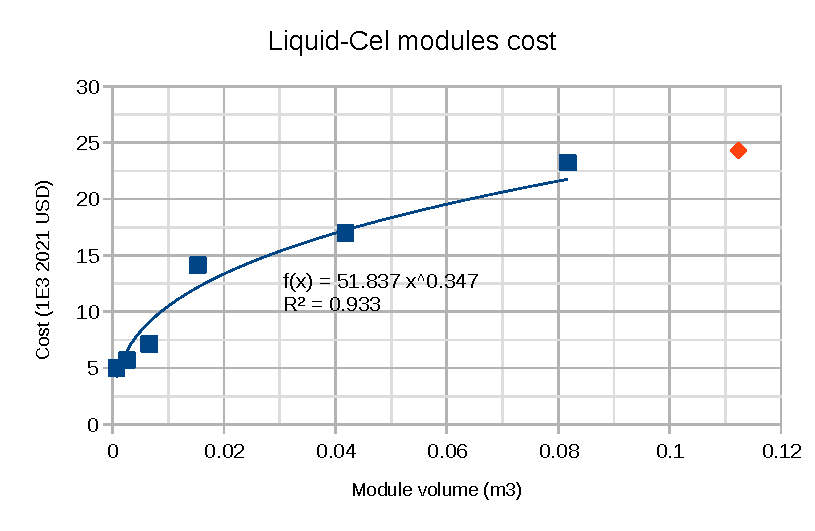
\includegraphics[width=0.6\linewidth, trim={0cm 0cm 0cm 0cm},clip]{MembranesCost.pdf} 
%	\caption{Estimation of Liquid-Cel\textsuperscript{\texttrademark} 14x40 membrane module cost.}
%	\label{fig:MembranesCost}
%\end{figure}

\begin{table}[h] 
\centering
\caption{Liquid-Cel\textsuperscript{\texttrademark} membranes size and cost \protect\citep{LiquidCelData, SGProjects, DPCWaterSolutions}.} \label{table:LiquidCelData}
\resizebox{\columnwidth}{!}{
%	\begin{threeparttable}
\begin{tabular}{@{}ccccc@{}}
	\toprule
	Membrane model & Flow capacity (m3/h) & Diameter (m) & Lenght (m) & Cost (USD) \\ \midrule
	2.5×8          & 0.1 - 0.7            & 0.067        & 0.200      & 5,000       \\
	4×13           & 0.5 - 3.4            & 0.116        & 0.242      & 5,700       \\
	8x20           & 1 - 11               & 0.219        & 0.406      & 14,150      \\
	10x28          & 10 - 48              & 0.279        & 0.683      & 17,000      \\
	%		14x28          & 16 - 91              & 0.356        & 0.821      & 23,200      \\
	14x40          & 16 - 125             & 0.356        & 1.129      & 24,300      \\ \bottomrule
\end{tabular}}
\end{table}

%\begin{table}[h] 
%	\centering
%	\caption{Main characteristics of Liquid-Cel \textsuperscript{\texttrademark} membrane \protect\citep{rongwong2020, ulbricht2013ammonia}.} \label{table:membrane_characteristichs}
%	%	\begin{threeparttable}
	%	\begin{tabular}{@{}cccc@{}}
		%		\toprule
		%		Membrane parameters  & Unit & Variable & Values  \\ \midrule
		%		Number of fibers     & $\frac{\text{fibers}}{\text{m}^2_{\text{module}}}$    & $n_f$       & $2.13 \cdot 10^6$    \\
		%		Fiber outer diameter & m    & $d_o$       & $300 \cdot 10^{-6}$  \\
		%		Fiber inner diameter & m    & $d_i$       & $240 \cdot 10^{-6}$  \\
		%		Pore diameter        & m    & $a$         & $0.04 \cdot 10^{-6}$ \\
		%		Porosity             & -    & $\varepsilon$  & 0.40     \\
		%		Tortuosity factor    & -    & $\tau$      & 2.60     \\
		%		Pressure drop shell side    & bar    & $\Delta P_{\text{shell side}}$      & 0.3     \\
		%		Pressure drop lumen side    & bar    & $\Delta P_{\text{lumen side}}$      & 2     \\
		%		\bottomrule
		%	\end{tabular}
	%\end{table}

Membrane sizing is performed through the membrane mass balances, {\color{blue}{Eqs. \ref{eq:Mem1}-\ref{eq:Mem26}.}} They are based on the distribution of ammonia species within the digestate, mass transfer on the digestate, wetted membrane, and non-wetted membrane phases, and the diffusion of ammonia through the membrane. Ammonia diffusion through the membrane is driven by bulk and Knudsen diffusivities, which consider the mean free path of molecules and the pore diameter respectively. Therefore, the cross-sectional area of the lumen and shell sides, as well as the lenght of the membrane are estimated based on mass balances, as shown in {\color{blue}{Eqs. \ref{eq:A_lumen}, \ref{eq:A_shell}, and \ref{eq:Mem27} of the Supplementary Material respectively.}}

%The main parameters for membrane modeling are calculated in {\color{blue}{Eqs. 
		%\ref{eq:Mem1}-\ref{eq:Mem99}
		%of the Supplementary Material}}, 
%including the cross-sectional area of the lumen and shell sides.
%Digestate density ($\rho$) and viscosity ($\mu$) were assumed equal to those of water.
%%Correlations to estimate these parameters are reported by \citet{hsu1997densities}.
%%Ammonia Henry's constant ($H_{\text{NH}_3}$)
%%%and  Knudsen diffusivity 
%%have been taken from \citet{linstrom2001}.
%%%and  \citet{agrahari2012ml} respectively. The correlations for the rest of parameters can be found in \citet{rongwong2020}:
%
%%\begin{align}
	%%& \rho_{\text{water}} \left(\frac{\text{kg}}{\text{m}^3}\right) = (10^3) \cdot \left(0.863559+1.21494 \cdot 10^{-3} \cdot T(\text{K}) - 2.5708 \cdot 10^{-6} \cdot T(\text{K})^2\right) \label{eq:Mem1} 
	%%\\
	%%& \mu_{\text{water}} \left(\frac{\text{kg}}{\text{m} \cdot \text{s}}\right) = (10^{-6}) \cdot \left(\rho \cdot e^{-3.28285+\frac{456.029}{T(\text{K})-154.576}}\right) \label{eq:Mem2} 
	%%\\
	%%& H_{\text{NH}_3} \left(\frac{\text{kmol}}{\text{atm} \cdot \text{m}^3}\right) = 58 \cdot e^{4100 \cdot \left(\frac{1}{T(\text{K})} - \frac{1}{298.15}\right)}
	%%\label{eq:Mem3}
	%%\end{align}
%
%%The cross-sectional area of the lumen area is calculated based on the transverse area of hollow fiber, and the number of fibers in the membrane module, Eq. \ref{eq:A_lumen} . Shell area is calculated as the difference between total and lumen side cross-sectional areas. 
%Velocities of digestate and stripping fluid (i.e., sulfuric acid solution) are computed based on their respective volumetric flow and transverse areas.
%
%%\begin{align}
	%%& n_{f_{\text{module}}} = A_{\text{module}} \cdot n_f \label{eq:Memnf} 
	%%\\
	%%& A_{\text{lumen side}} \left(\text{m}^2\right) = \frac{d_i^2}{4} \cdot \pi \cdot n_{f_{\text{module}}} \label{eq:A_lumen} 
	%%\\
	%%& A_{\text{shell side}} \left(\text{m}^2\right) = \frac{D_{\text{module}^2}}{4} \cdot \pi - A_{\text{lumen side}} \label{eq:A_shell} 
	%%\\
	%%& V_{\text{stripping fluid}} \left(\frac{\text{m}}{\text{s}}\right) = \frac{\dot{V}_{\text{stripping fluid}}}{A_{\text{lumen side}}} \label{eq:V_stripping}
	%%\\
	%%& V_{\text{digestate}} \left(\frac{\text{m}}{\text{s}}\right) = \frac{\dot{V}_{\text{digestate}}}{A_{\text{shell side}}} \label{eq:V_digestate}
	%%\end{align}
%
%%Diffusion of ammonia through the membrane is driven by bulk and Knudsen diffusivities, which consider the mean free path of molecules and the pore diameter respectively. Bulk diffusivity of ammonia is calculated based on the kinetic theory, using Eq. \ref{eq:Mem5}, while Knudsen diffusivity depends on the molecular velocity, Eq. \ref{eq:Mem4}, and pore diameter, Eq. \ref{eq:Mem7} \citet{agrahari2012ml}. Both contributions to ammonia transport are combined in a effective diffusion coefficient, Eq. \ref{eq:Mem88}. Ammonia diffusion in liquid phase has been assumed equal to ammonia diffusion in water, which is calculated using Eq. \ref{eq:Mem99}. 
%
%The diffusion of ammonia through the membrane is driven by bulk and Knudsen diffusivities, which consider the mean free path of molecules and the pore diameter respectively. Both contributions to ammonia transport are combined in a effective diffusion coefficient, as shown in Eq. \ref{eq:Mem88Manuscript}. Bulk diffusivity of ammonia is calculated based on the kinetic theory,
%%using Eq. \ref{eq:Mem5}, 
%while Knudsen diffusivity depends on the molecular velocity
%%, Eq. \ref{eq:Mem4}, 
%and pore diameter, as shown in {\color{blue}{Eqs. \ref{eq:Mem5} to \ref{eq:Mem99} of the Supplementary Material}}
%%, Eq. \ref{eq:Mem7}
%\citep{agrahari2012ml}.
%%Both contributions to ammonia transport are combined in a effective diffusion coefficient, Eq. \ref{eq:Mem88Manuscript}. Ammonia diffusion in liquid phase has been assumed equal to ammonia diffusion in water, which is calculated using Eq. \ref{eq:Mem99Manuscript}. 
%
%\begin{align}
	%%& \bar{v}  \left(\frac{\text{m}}{\text{s}}\right) = \left(\frac{8 \cdot R\left(\frac{\text{J}}{\text{mol} \cdot \text{K}}\right) \cdot T\left(\text{K}\right)}{MW_{\text{NH}_3} \left(\frac{\text{kg}}{\text{mol}}\right) \cdot \pi} \right)^{\sfrac{1}{2}}
	%%\label{eq:Mem4} 
	%%\\
	%%& D_{\text{NH}_{3}}  \left(\frac{\text{m}^2}{\text{s}}\right) = \frac{1}{3} \cdot \lambda \cdot \bar{v}
	%%\label{eq:Mem5} 
	%%\\
	%%& \lambda  \left(\text{m}\right) = \frac{\kappa \left(\frac{\text{J}}{\text{K}}\right) \cdot T\left(\text{K}\right)}{\pi \cdot \sigma_{\text{NH}_3}^2 \left(\text{m}^2\right) \cdot P\left(\text{Pa}\right) \cdot 2^{\sfrac{1}{2}}}
	%%\label{eq:Mem6} 
	%%\\
	%%& D_{\text{NH}_{3_\text{Kn}}} \left(\frac{\text{m}^2}{\text{s}}\right) = \frac{d_{\text{pore}}}{3} \cdot \left(\frac{8 \cdot R\left(\frac{\text{J}}{\text{mol} \cdot \text{K}}\right) \cdot T(\text{K})} {\pi \cdot MW_{\text{NH}_3} \left(\frac{\text{kg}}{\text{mol}}\right)} \right)^{\sfrac{1}{2}}
	%%\label{eq:Mem7}
	%%\\
	%& D_{\text{eff}} \left(\frac{\text{m}^2}{\text{s}}\right) = \frac{1}{\frac{1}{D_{\text{NH}_{3_\text{Kn}}}} + \frac{1}{D_{\text{NH}_{3}}}}
	%\label{eq:Mem88Manuscript}
	%%\\
	%%& D_{\text{NH}_{3_\text{water}}} \left(\frac{\text{m}^2}{\text{s}}\right) = 1.96 \cdot 10^{-9} \cdot \frac{\mu_{\text{water}_{T=298\text{K}}}}{\mu_{\text{water}_{T}}} \cdot \frac{T\left(\text{K}\right)}{298}
	%%\label{eq:Mem99Manuscript}
	%\end{align}
%
%The distribution of ammonia species shown in Eq. \ref{eq:NH3NH4} is calculated at initial conditions based on the pH of the digestate stream being fed through the tube side of the membrane module, which is assumed equal to 11, as shown in Eq. \ref{eq:Mem9Manuscript}.
%% \ref{eq:Mem11Manuscript}-\ref{eq:Mem10Manuscript}.
%
%\begin{align}
	%%&  f_{\text{NH}_3} = \frac{1}{10^{\left(pK_{a_{\text{NH}_3}}-pH\right)}+1} \label{eq:Mem8} 
	%%\\
	%%&  pK_{a_{\text{NH}_3}} \left(\frac{\text{kmol}}{\text{m}^3}\right) = 0.0901821+\frac{2729.92}{T(\text{K})} \label{eq:Mem11Manuscript} 
	%%\\
	%%&  \left[{\text{NH}_3}\right] = \left[{\text{N}_\text{inorg}}\right] \cdot f_{\text{NH}_3} \label{eq:Mem9} 
	%&  \left[{\text{NH}_3}\right] = \left[{\text{N}_\text{inorg}}\right] \cdot \frac{1}{10^{\left(pK_{a_{\text{NH}_3}}-pH\right)}+1} \label{eq:Mem9Manuscript} 
	%%\\
	%%&  \left[{\text{NH}_4^+}\right] = \left[{\text{N}_\text{inorg}}\right] \cdot \left(1-\frac{1}{10^{\left(pK_{a_{\text{NH}_3}}-pH\right)}+1}\right) \label{eq:Mem10Manuscript} 
	%%&  \left[{\text{NH}_4^+}\right] = \left[{\text{N}_\text{inorg}}\right] \cdot \left(1-f_{\text{NH}_3}\right) \label{eq:Mem10}
	%%\\
	%%&  \left[{\text{H}^+}\right] = K_a \cdot \frac{\left[{\text{NH}_4^+}\right]}{\left[{\text{NH}_3}\right]} \label{eq:Mem12} 
	%\end{align}
%
%%A modified Henry's constant considering the speciation of ammonia is used in the model proposed by \citet{rongwong2020} to evaluate the liquid-solid equilibrium of ammonia, Eq. \ref{eq:Mem13Manuscript}.
%%
%%\begin{align}
	%%&  H_{\text{NH}_3}^* = H_{\text{NH}_3} \cdot \left(1+\frac{K_a \cdot \left[{\text{H}^+}\right]}{Kw}\right) \label{eq:Mem13Manuscript}  
	%%\end{align}
%
%The mass transfer coefficient of the digestate flowing in the tube side, $k_{\text{digestate}}$, is calculated through the Sherwood number of this stream, Eq. \ref{eq:Mem14Manuscript}.
%%and Eqs. \ref{eq:Mem15} and \ref{eq:Mem16}.
%
%\begin{align}
	%&  \text{Sh}_{\text{digestate}} = \frac{k_{\text{digestate}} \cdot d_i}{D_{\text{NH}_{3_\text{water}}}} = 1.62 \cdot \left(\frac{d_i}{L} \cdot \text{Re}_{\text{digestate}} \cdot \text{Sc}_{\text{digestate}}\right)^{\sfrac{1}{3}} \label{eq:Mem14Manuscript}
	%%\\
	%%&  \text{Re}_{\text{digestate}} = \frac{d_i \cdot \rho_{\text{digestate}} \cdot V_{\text{digestate}}}{\mu_{\text{digestate}}} \label{eq:Mem15}
	%%\\
	%%&  \text{Sc}_{\text{digestate}} = \frac{\mu_{\text{digestate}}}{\rho_{\text{digestate}} \cdot D_{\text{NH}_{3_\text{water}}}} \label{eq:Mem16}
	%\end{align}
%
%%The membrane phase can be divided into non-wetted and wetted membrane sections. Their mass transfers coefficients, $k_M$ and $k_M^{'}$ respectively, are calculated based on the fraction of membrane wetted by the digestate. This is calculated based on a correlation reported by \citet{rongwong2020}, shown in Eq. \ref{eq:Mem20}. Eqs. \ref{eq:Mem17}-\ref{eq:Mem18} and \ref{eq:Mem21}-\ref{eq:Mem22} shown the equations employed for the estimation of $k_M$ and $k_M^{'}$ respectively.
%%\begin{align}
	%%& w_{\text{membrane}} = \frac{0.368}{2.709 + e^{-17.486 \cdot \left(V_{\text{digestate}}-0.25\right)}} \label{eq:Mem20}
	%%\\
	%%& d_{\text{interfacial}} \left(\text{m}\right) = d_i + w_{\text{membrane}} \cdot \left(d_o-d_i\right) \label{eq:Mem19}
	%%\\
	%%&  k_M \left(\frac{\text{m}}{\text{s}}\right) = \frac{D_{\text{eff}} \cdot \varepsilon}{\tau \cdot \delta_{\text{non-wetted}}} \label{eq:Mem17}
	%%\\
	%%& \delta_{\text{non-wetted}} \left(\text{m}\right) = \frac{d_o-d_{\text{interfacial}}}{2} \label{eq:Mem18}
	%%\\
	%%&  k_M^{'} \left(\frac{\text{m}}{\text{s}}\right) = \frac{D_{\text{water}} \cdot \varepsilon}{\tau \cdot \delta_{\text{wetted}}} \label{eq:Mem21}
	%%\\
	%%& \delta_{\text{wetted}} \left(\text{m}\right) = \frac{d_{\text{interfacial}}-d_i}{2} \label{eq:Mem22}
	%%\end{align}
%
%%The overall mass transfer coefficient is calculated based on the liquid, wetted membrane, and non-wetted membranes mass transfer coefficients, as shown in Eq. \ref{eq:Mem23}. However, high ammonia concentrations result in a decrease of the overall mass transfer \citep{zhu2005}. Therefore, $K_{ov}$ is modified using a correction factor that consider the concentration of ammonia in digestate.
%
%The overall mass transfer coefficient Eq. \ref{eq:Mem23Manuscript} is calculated based on the liquid, wetted membrane, and non-wetted membranes mass transfer coefficients, calculated in {\color{blue}{Eqs. \ref{eq:Mem17} and \ref{eq:Mem21}}}. However, high ammonia concentrations result in a decrease of the overall mass transfer \citep{zhu2005}. Therefore, $K_{ov}$ is modified using a correction factor that consider the concentration of ammonia in digestate, Eq. \ref{eq:KovCorrectedManuscript}.
%
%\begin{align}
	%& K_{ov} \left(\frac{\text{m}}{\text{s}}\right) = \frac{1}{\left(\frac{1}{k_{\text{digestate}} \cdot d_i} + \frac{1}{k_M^{'} \cdot \delta_{\text{ln wetted}}} + \frac{R \left(\frac{\text{atm} \cdot \text{m}^3}{\text{kmol} \cdot \text{K}}\right) \cdot T(\text{K}) \cdot H_{\text{NH}_3}^{*}}{k_M \delta_{\text{ln non-wetted}}}\right) \cdot d_o } \label{eq:Mem23Manuscript}
	%\\
	%& \delta_{\text{ln wetted}} = \frac{d_{\text{interfacial}}-d_i}{\text{ln}\left( \frac{d_{\text{interfacial}}}{d_i}\right)} \label{eq:Mem24Manuscript}
	%\\
	%& \delta_{\text{ln non-wetted}} = \frac{d_o - d_{\text{interfacial}}}{\text{ln}\left( \frac{d_o}{d_{\text{interfacial}}}\right)} \label{eq:Mem25Manuscript}
	%\\
	%& K_{ov_{\text{corrected}}} \left(\frac{\text{m}}{\text{s}}\right) = K_{ov} \cdot \left(1-\frac{0.002728 \cdot \left[\text{NH}_3\right] \left(\frac{\text{mg}}{\text{L}}\right)}{100}\right) \label{eq:KovCorrectedManuscript}
	%\end{align}
%
%%The mass balance along the membrane can be performed considering the mass transfer in an infinitesimal element of the membrane, as shown in Eq. \ref{eq:Mem26}. Due to the excess of sulfuric acid in the lumen side that lead the formation of ammonium sulfate from the ammonia recovered, the concentration of ammonia in the lumen side is assumed negligible. This differential expression can be analytically integrated to estimate the total length of the membrane, Eq. \ref{eq:Mem27}.
%
%The total length of the membrane can be estimated through Eq. \ref{eq:Mem27Manuscript}, which is obtained from The mass balance along the membrane considering the mass transfer in an infinitesimal element of the membrane, shown in Eq. \ref{eq:Mem26}.
%
%\begin{align}
	%%\frac{\dot{n}_{\text{NH}_3}}{dz} &= -n_{f_{\text{module}}} \cdot \pi \cdot d_o \cdot K_{{ov}_\text{corrected}} \cdot \left( \frac{\dot{n}_{\text{NH}_3}}{\dot{V}_{\text{digestate}}} - \frac{ H_{\text{NH}_3}^* \cdot p_{\text{NH}_3}}{\dot{V}_{\text{digestate}}}\right) \nonumber
	%%\\ 
	%%& \approx -n_{f_{\text{module}}} \cdot \pi \cdot d_o \cdot K_{{ov}_\text{corrected}} \cdot \frac{\dot{n}_{\text{NH}_3}}{\dot{V}_{\text{digestate}}} \label{eq:Mem26}
	%%\\
	%& z \left(\text{m}\right) = \text{ln}\left(\frac{\dot{n}_{\text{NH}_{3_{final}}}}{\dot{n}_{\text{NH}_{3_{initial}}}}\right) \cdot \frac{\dot{V}_{\text{digestate}}}{-n_{f_{\text{module}}} \cdot \pi \cdot d_o \cdot K_{{ov}_\text{corrected}}} \label{eq:Mem27Manuscript}
	%\end{align}

One or multiple membrane modules can be needed to achieve the total membrane length $\left( z \right)$ needed to reach a certain efficiency, as shown in Eq. \ref{eq:nserie}. $n_{\text{series}}$ denotes the necessary number of membrane units of length $L_{\text{module}}$ in-series arrangement to achieve the desired recovery efficiency. The length of the different membrane units is reported in Table \ref{table:LiquidCelData}. $n_{\text{parallel}}$ refers to the number of membrane units in-parallel arrangement required to process the waste flow generated at the livestock facility under study based on the processing capacities reported in Table \ref{table:LiquidCelData}. Membrane modules CAPEX is estimated through Eq. \ref{eq:CAPEXmembrane}, assuming a membrane lifetime $\left(t_{\text{module}}\right)$ of 10 years \citep{verrecht2010cost}, and a plant lifetime $\left(t_{\text{plant}}\right)$ of 20 years. The use of sulfuric acid as stripping fluid and membrane cleaning is the main contributor to membrane OPEX, as shown in Eq. \ref{eq:OPEXmembrane}. Membrane cleaning cost $\left(c_{\text{cleaning}}\right)$ is reported to be between 2\% and 25\% of the operating costs \citep{yu2020performance, verrecht2010cost}, for which we assume an average value of 13.5\%. 
Additionally, the cost of the pumps needed for driving the digestate and stripping fluid streams through the membrane modules is considered. Cost estimation of pumps is collected in {\color{blue}{Eqs. \ref{eq:n_pumps} to \ref{eq:pumpsOPEX} of the Supplementary Material.}}

\begin{align}
	& n_{\text{series}} = \ceil*{\frac{z}{L_{\text{module}}}} \label{eq:nserie}
	\\
	& CAPEX_{\text{membranes}} \left(\text{2019 USD}\right)= \left(n_{\text{serie}} \cdot n_{\text{parallel}}\right) \cdot \nonumber \\
	& Cost_{\text{module}} \left(\frac{\text{USD}}{\text{module}}\right) \cdot \frac{t_{\text{plant}}}{t_{\text{module}}} \label{eq:CAPEXmembrane}
	\\
	& OPEX_{\text{membranes}} \left(\frac{\text{2019 USD}}{\text{year}}\right) = \nonumber \\
	& \frac{\dot{m}_{\text{H}_2 \text{SO}_4} \left(\frac{\text{kg}}{\text{s}}\right)}{\rho_{\text{H}_2 \text{SO}_4} \left(\frac{\text{kg}}{\text{m}^3}\right)} \cdot Price_{\text{H}_2 \text{SO}_4} \left(\frac{\text{USD}}{\text{m}^3}\right) \cdot \frac{1}{1-\frac{c_{\text{cleaning}}}{100}} \label{eq:OPEXmembrane}
\end{align}

%Additionally, pumps to drive the digestate and stripping fluid streams are needed. Their cost is estimated using Eqs. \ref{eq:n_pumps} and \ref{eq:pumpsCAPEX}, assuming that the maximum capacity of one single pump $\left(\dot{V}_{\text{pump}_{\text{max}}}\right)$ is 1 $\sfrac{\text{m}^3}{\text{s}}$ \citep{peters2003plant}. Pumps operating cost are estimated through Eqs. \ref{eq:pumpsH} to \ref{eq:pumpsOPEX}, calculating the energy needed to balance the pressure drop of the shell and lumen sides of the membrane, Table \ref{table:membrane_characteristichs}. Pump efficiencies $\left(\eta_{\text{pump}_i}\right)$ of 0.8 are assumed.
%\begin{align}	
	%&
	%n_{\text{pump}_i} = \ceil*{\frac{\dot{V}_i}{\dot{V}_{\text{pump}_{\text{max}}}}} \label{eq:n_pumps}
	%\\
	%& CAPEX_{\text{pumps}_i} \left(\text{2019 USD}\right) =
	%\begin{cases}
		%(-50.387\cdot10^6 \cdot \dot{V}_i^2 + 1.607\cdot10^6 \cdot \dot{V}_i 
		%\\
		%+ 5.127\cdot10^3) \cdot n_{\text{pump}_i} \cdot 1.055 & \text{if } \dot{V}_i \leq 9\cdot10^{-3} \frac{\text{m}^3}{\text{s}}  \\
		%(92.562\cdot10^3\cdot \dot{V}_i^{0.381}) \cdot n_{\text{pump}_i} \cdot 1.055 & \text{if }  \dot{V}_i > 9\cdot10^{-3} \frac{\text{m}^3}{\text{h}}
		%\end{cases} \label{eq:pumpsCAPEX} \\ 
	%& H_i \left(\text{m}\right) = \frac{\Delta P_i \left(\text{Pa}\right)}{\rho \left(\frac{\text{kg}}{\text{m}^3}\right) g\left(\frac{\text{m}}{\text{s}^2}\right)} \label{eq:pumpsH}
	%\\
	%& \dot{W}_{\text{pump}_i} \left(\text{kW}\right) = \frac{g\left(\frac{\text{m}}{\text{s}^2}\right) \cdot H_i \left(\text{m}\right) \cdot \rho \left(\frac{\text{kg}}{\text{m}^3}\right) \cdot \dot{V}_i \left(\frac{\text{m}^3}{\text{s}}\right)}{\eta_{\text{pump}_i}} \label{eq:pumpsPower}
	%\\
	%& OPEX_{\text{pumps}} \left(\frac{\text{2019 USD}}{\text{year}}\right) = \sum_{i} \dot{W}_{\text{pump}_i} \left(\text{kW}\right) \cdot t_{\text{operation}} \left(\text{s}\right) \cdot 3600 \cdot Price_{\text{electricity}}\left(\frac{\text{USD}}{\text{kWh}}\right) \label{eq:pumpsOPEX}
	%\\
	%& \forall \ i  \in \{\text{shellside, lumenside}\} \nonumber 
	%\end{align}

Total capital and operating expenses for the recovery of nitrogen from livestock digestate using a transmembrane chemisorption process result from the sum of membrane and pump costs are described in Eqs \ref{eq:CAPEX_Transmem} and \ref{eq:OPEX_Transmem}.

\begin{align}	
	& CAPEX_{\substack{\text{transmembrane} \\ \text{chemisorption}}}	= CAPEX_{\text{membranes}} + \sum_{\mathclap{\substack{i 
				\in \\
				\{\text{shellside,} \\ 
				\text{lumenside}\}}}} CAPEX_{\text{pumps}_i} \label{eq:CAPEX_Transmem}
	\\
	& OPEX_{\substack{\text{transmembrane} \\ \text{chemisorption}}}	= OPEX_{\text{membranes}} + OPEX_{\text{pumps}} \label{eq:OPEX_Transmem}
\end{align}	


%\paragraph{\textbf{Ammonia evaporation}} \label{section:Digestate dryingNrecovery}

\textbf{Ammonia evaporation:} Nitrogen can be recovered by ammonia evaporation through digestate drying in a belt dryer unit. The operation of a belt dryer unit requires a minimum concentration of solids of 10\% - 12\% \citep{bolzonella2018nutrients}. Therefore, the liquid and solid outlet streams from the solid-liquid separation stage are combined to obtain a stream with the desired solids content. After solids content adjustment, digestate is dried in the belt drier, as shown in Fig \ref{fig:BeltDryerScheme}. This unit drys the digestate over the belt with a stream of hot air crossing the belt through orifices on it. Heat (sensible and latent) is transferred from the hot air to the digestate on the belt
%in the form of sensible heat, devoted 
to increase temperature
%increase, and latent heat, devoted 
%to the evaporation  
%As a result, 
and evaporate
ammonia and a fraction of moisture.
%+are evaporated. 
%Since the amount of ammonia in digestate is significantly lower than moisture, air saturation with water vapor is considered the evaporation limit. It must be noted that the moisture carrying capacity of air (i.e., the saturation point) is a function of temperature. 
%Therefore, mass and energy balances must be performed simultaneously to determine the amount of ammonia and water carried by the air stream, as well as the final temperature of this stream. 
%An ammonia evaporation yield of 80\% has been assumed based on experimental data \citep{awiszus2018ammonia}. 

%\begin{figure}[h]
%	\centering
%	%	\begin{subfigure}[t]{0.5\linewidth}
%	\includegraphics[width=1\linewidth, trim={0cm 0cm 0cm 0cm},clip]{BeltDryerFinal3.pdf} 
%	\caption{Belt dryer scheme.}
%	\label{fig:BeltDryerScheme}
%\end{figure}

The belt dryer model assumes the evaporation of two components in no equilibrium with a continous extraction of the vapour phase \citep{treybal1980mass}.
%, Eq. \ref{eq:BD11} , 
Since the amount of ammonia in digestate is significantly lower than moisture, air saturation with water vapor is considered the evaporation limit. It must be noted that the moisture carrying capacity of air (i.e., the saturation point) is a function of temperature. This requires to solve the mass and energy balances simultaneously, which are reported in the {\color{blue}{Supplementary Material
%, which are simultaneously solved with the mass balances,
Eqs.
%\ref{eq:BD15} and Eqs.\ref{eq:BD1}-
%\ref{eq:BD11Manuscript}-\ref{eq:BD1Manuscript}
shown in Eqs. \ref{eq:BD11}-\ref{eq:BD10}.}}
%The calculation of the different contributions to energy balances are reported in the {\color{blue}{Supplementary Material, Eqs. \ref{eq:BD2} to \ref{eq:BD10}.}}
%\ref{eq:BD10}.
An ammonia removal efficiency $\left(\eta_{\text{belt dryer}}\right)$ of 80\% has been assumed for mass balances calculation
%, Eq. \ref{eq:BD11Manuscript}
\citep{awiszus2018ammonia}.
%respectively. 
%Air saturation by moisture, Eq. \ref{eq:BD13Manuscript}, and ammonia, Eq. \ref{eq:BD15Manuscript}, represent the upper bound to the carry of these compounds in the air stream. 
The assumptions for the modeling of ammonia evaporation by digestate drying are collected in {\color{blue}{the Section \ref{section:DigDryingNRecoveryPaper} of the Supplementary Material}}.
%The amount of ammonia recovered by evaporation is computed through Eq. \ref{eq:BD11}. 
%The following assumptions has been made for the modeling of digestate drying:
%\begin{itemize}
%	\item $c_{p_{\text{digestate}_{\text{in}}}} \approx c_{p_{\text{water}}}$
%	\item $P_{\text{water}} + P_{\text{NH}_3} \approx P_{\text{water}}$
%	\item $T_{\text{out}_{\text{air}}} = T_{\text{out}_{\text{digestate}}}$
%	\item $\alpha = \text{constant}$
%\end{itemize}

%\begin{align}
%%	& \alpha \cdot \text{ln}\frac{\dot{n}_{\text{water}_\text{in}}}{\dot{n}_{\text{water}_\text{out}}} =  \text{ln}\frac{\dot{n}_{\text{NH\textsubscript{3}}_\text{in}}}{\dot{n}_{\text{NH\textsubscript{3}}_\text{out}}} \label{eq:BD11} 
%%	\\
%%	& \alpha =  \frac{Pv_{\text{NH}_3} \left(T\right)}{Pv_{\text{water}} \left(T\right)} \label{eq:BD12} 
%%	\\
%&\dot{m}_{\text{NH}_{3\text{ evap}}} = \dot{m}_{\text{NH}_{3\text{ in}}} \cdot \eta_{\text{belt dryer}}^{\text{NH}_3} \label{eq:BD11Manuscript} 
%\\
%& \frac{\frac{\dot{m}_{\text{water}_\text{evap}}}{MW_{\text{water}}}}{\sum_{j}\frac{\dot{m}_j}{MW_j}} \cdot P_{\text{total}} \leq Pv_{\text{water}} \left(T\right) \label{eq:BD13Manuscript} 
%\\
%%	& P_{\text{water}} =  \dot{n}_{\text{water}_\text{evap}} \cdot P_{\text{total}} \label{eq:BD14} 
%%	\\
%&\frac{\frac{\dot{m}_{\text{NH}_{3\text{ evap}}}}{MW_{\text{NH}_3}}}{\sum_{j}\frac{\dot{m}_j}{MW_j}} \leq Pv_{\text{NH}_3} \left(T\right) \label{eq:BD15Manuscript} 
%\\
%& \forall \ j \ \in \ \{\text{air}, \ \text{H\textsubscript{2}O}, \ \text{NH}_3\} \nonumber
%%\end{align}
%%
%%\begin{align}
%\\
%& \dot{Q}_{\text{Belt Dryer}} = \dot{H}_{\text{latent}} + \dot{H}_{\text{sensible}} = \dot{H}_{\text{air}_{\text{in}}} - \dot{H}_{\text{air}_{\text{out}}} \label{eq:BD1Manuscript} 
%%\\
%%& \dot{H}_{\text{latent}} = \dot{m}_{\text{water}_\text{evap}} \cdot \lambda_{\text{evap}_{\text{water}}}\left(T\right) + \dot{m}_{\text{NH}_{3_\text{evap}}} \cdot \lambda_{\text{evap}_{\text{NH}_3}}\left(T\right) \label{eq:BD2} 
%%\\
%%& \dot{H}_{\text{sensible}} = \dot{H}_{\text{digestate}_\text{out}} - \dot{H}_{\text{digestate}_\text{in}} + \dot{H}_{\text{sensible}_{\text{gases}}} \label{eq:BD3} \\
%%& \dot{H}_{\text{sensible}_{\text{gases}}} = \left( \dot{m}_{\text{water}_\text{evap}} + \dot{m}_{\text{NH}_{3_\text{evap}}} \right) \cdot c_{p_{\text{water (liquid)}}} \cdot T_{\text{air}_\text{out}} \label{eq:BD4} 
%%\\
%%& \dot{H}_{\text{digestate}_{\text{in}}} = \dot{m}_{\text{digestate}_{\text{in}}} \cdot c_{p_{\text{water}}} \cdot \Delta T_{\text{digestate}_\text{in}} \label{eq:BD5} 
%%\\
%%& \dot{H}_{\text{digestate}_{\text{out}}} = \dot{m}_{\text{digestate}_{\text{out}}} \cdot c_{p_{\text{digestate}}} \cdot \Delta T_{\text{digestate}_\text{out}} \label{eq:BD6} 
%%\\
%%& c_{p_{\text{digestate}}} \left(\sfrac{kg}{kJ \cdot K}\right)= 4.19-0.0275 \cdot \left(\frac{\dot{m}_{\text{TS}_{\text{out}}}}{\dot{m}_{\text{digestate}_{\text{out}}}} \cdot 100 \right) \label{eq:BD7} 
%%\\	
%%& \dot{H}_{\text{air}_{\text{in}}} = \dot{m}_{\text{air}} \cdot c_{p_{\text{air}}} \cdot \Delta T_{\text{air}_\text{in}} \label{eq:BD8} 
%%\\	
%%& \dot{H}_{\text{air}_{\text{out}}} = \left(\dot{m}_{\text{air}} \cdot c_{p_{\text{air}}} + \dot{m}_{\text{water}_\text{evap}} \cdot c_{p_{\text{water (gas)}}} + \dot{m}_{\text{NH}_{3_\text{evap}}} \cdot c_{p_{\text{NH\textsubscript{3} (gas)}}} \right) \cdot \Delta T_{\text{air}_\text{out}} \label{eq:BD9} 
%%\\	
%%& \Delta T_i = T_i - T_\text{ref} \ \forall \ i \ \in \ \{\text{air}_\text{in}, \ \text{air}_\text{out},  \ \text{digestate}_\text{in}, \ \text{digestate}_\text{out} \} \label{eq:BD10}
%\end{align}

Gaseous ammonia is further recovered through acidic scrubbing, as described in Section \ref{section:scrubbing}. 

Capital expenses estimation for belt dryer units is based on the energy required for ammonia evaporation.
%digestate drying.
A drying efficiency $\left(\eta_{\text{belt dryer}}\right)$ of 0.6 has been assumed from the experimental work reported by \citet{awiszus2018utilization}. Belt dryer scale-up is based on the correlation proposed by \citet{towler2012chemical}, as shown in Eq. \ref{eq:CAPEXBeltDryer}. The reference values and scale factor used in this correlation are taken from costs and capacities reported by \citet{turley2016assessment}, as well as the maximum belt dryer capacity used to compute the number of dryer units needed $\left(n_{\text{belt dryer}} \right)$ , as shown in Eq. \ref{eq:nBeltDryer}. These data are also used to estimate the scale-up factor, which is estimated equal to 0.7. Belt dryer operating costs are due to electrical consumption, which has been estimated in 0.099 kW of electricity per kW of thermal energy used by the unit, as shown in Eq. \ref{eq:BeltDryerOPEX} \citep{awiszus2018utilization}.

\begin{align}
%	&
%	\frac{\dot{m}_{\text{water}_\text{evap}}}{t_{\text{operation}}}  
%	\\
& \dot{Q}_{\text{belt dryer}}^{\text{real}} = \frac{\dot{Q}_{\text{belt dryer}}\left(\text{kW}\right)}{\eta_{\text{belt dryer}}} \label{eq:QeltDryerReal} 
\\
& n_{\text{belt dryer}} = \ceil*{\frac{\dot{Q}_{\text{belt dryer}}^{\text{real}}\left(\text{kW}\right)}{1000}} \label{eq:nBeltDryer} 
\\
& \dot{Q}_{\text{belt dryer}}^{\text{design}} = \frac{\dot{Q}_{\text{belt dryer}}^{\text{real}}}{n_{\text{belt dryer}}} \label{eq:QeltDryerDesign} 
\\
& CAPEX_{\text{belt dryer}} \left(\text{2019 USD}\right) = \nonumber \\
& \left(n_{\text{belt dryer}} \cdot 214,997 \cdot \left(\frac{\dot{Q}_{\text{belt dryer}}^{\text{design}}\left(\text{kW}\right)}{500}\right)^{0.7}\right) \cdot 1.216 \label{eq:CAPEXBeltDryer} 
\\
& OPEX_{\text{belt dryer}} \left(\frac{\text{2019 USD}}{\text{year}}\right) = n_{\text{belt dryer}} \cdot \dot{Q}_{\text{belt dryer}}^{\text{design}} \left(\text{kW}\right) \cdot 0.099 \left(\frac{\text{kW}_{\text{e}}}{\text{kW}_{\text{t}}}\right) \cdot \label{eq:BeltDryerOPEX}
\\ 
& t_{\text{operation}} \left(\text{s}\right) \cdot 3600 \cdot Price_{\text{electricity}} \left(\frac{\text{USD}}{\text{kWh}}\right)  \nonumber
\end{align}

%\paragraph{\textbf{Stripping in packed tower}} \label{section:StrippingNrecovery}
\textbf{Stripping in packed tower:} Nitrogen recovery by stripping of the liquid digestate is a widely used technique based on the transfer of ammonia from liquid digestate to an air stream. This operation can be performed either in packed towers or in bubble column reactors, see Section \ref{section:bubblestripping}. Gaseous ammonia is further recovered through acidic scrubbing, as described in Section \ref{section:scrubbing}.

Nitrogen recovery using packed tower stripping, illustrated in Figure \ref{fig:ScrubberScheme}, has been modeled using the number of transfer units (NTU) method \citep{Metcalf}. The pressure drop of tower packing is estimated through the correlation proposed by \citet{kister1991predict}, as shown in Eq. \ref{eq:PDrop}. 

%\begin{figure}[h]
%	\centering
%	%	\begin{subfigure}[t]{0.5\linewidth}
%	\includegraphics[width=0.8\linewidth, trim={0cm 0cm 0cm 0cm},clip]{StrippingScrubbing.pdf} 
%	\caption{Stripping and scrubber towers scheme.}
%	\label{fig:ScrubberScheme}
%\end{figure}

\begin{align}
& P \left(\frac{\text{inch water}}{\text{ft}}\right) = 0.115 \cdot \left( F_{P}  \left(\text{ft}^{-1}\right)\right) ^{0.7} \label{eq:PDrop}
\end{align}

The tower diameter is calculated through the tower flooding capacity. A tower flooding capacity correlation considering the packing pressure drop is developed using ALAMO \citep{wilson2017alamo} based on the flooding curves developed by \citet{strigle1994packed}, as shown in Eq. \ref{eq:FloodingALAMO} and Figure \ref{fig:FloodingALAMO}. Two-inch (0.051 m) Intalox packing is considered \citep{strigle1994packed}, which packing factor $\left(F_P\right)$ is assumed to be 
18 ft\textsuperscript{-1}
(59 m\textsuperscript{-1})
\citep{geankoplis2003transport}. The operating line considered, defined as the ratio of gas and liquid volumetric flows, can be computed through Eqs. \ref{eq:FloodingALAMO} to \ref{eq:OpLine},
where $v_G$ denotes the superficial gas velocity in $\left(\frac{\text{ft}}{\text{s}}\right)$, $\rho_G$ the gas density in $\left(\frac{\text{lb}}{\text{ft}^3}\right) $, $\rho_L$ the liquid density in $ \left(\frac{\text{lb}}{\text{ft}^3}\right) $, $\nu$  the kinematic viscosity in $\left(\text{censtokes}\right)$, $G_G$the gas mass velocity in $\left(\frac{\text{lb}}{\text{ft}^2 \cdot \text{s}}\right)$, and $G_L$ the liquid mass velocity in $\left(\frac{\text{lb}}{\text{ft}^2 \cdot \text{s}}\right) $
\citep{strigle1994packed}.
%, defined as the ratio of gas and liquid volumetric flows, is assumed to be 2668 m\textsuperscript{3}\textsubscript{gas}/m\textsuperscript{3}\textsubscript{liquid} \citep{strigle1994packed}.

\begin{figure}[h!]
\centering
%	\begin{subfigure}[t]{0.5\linewidth}
	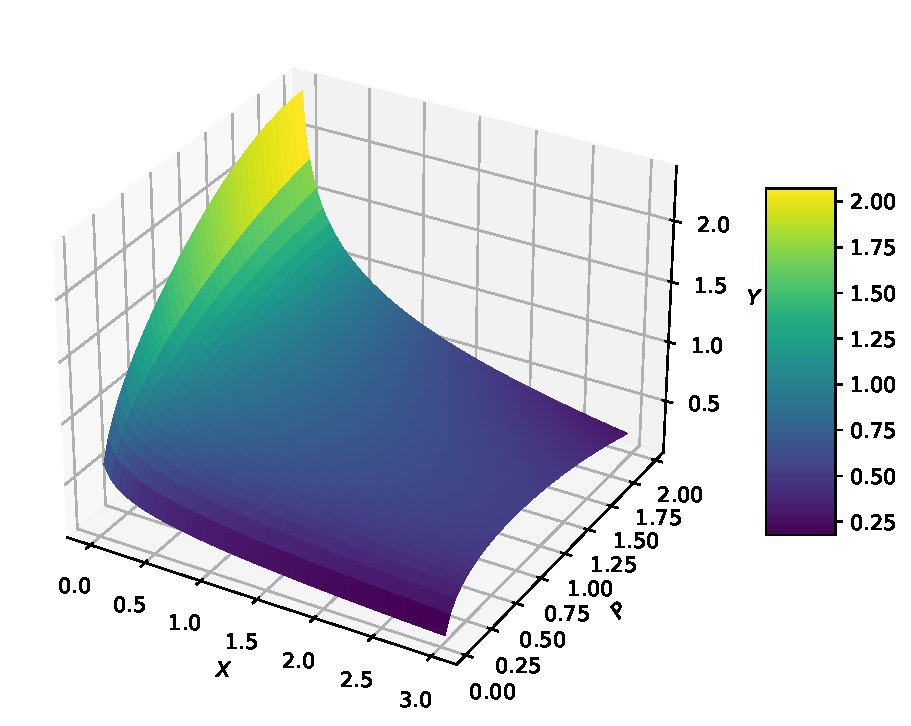
\includegraphics[width=0.72\linewidth, trim={1cm 0cm 0cm 1cm},clip]{gfx/Chapter6/AlamoFlooding.pdf} 
	\caption{Tower flooding capacity correlation considering packing pressure drop.}
	\label{fig:FloodingALAMO}
\end{figure}

%\begin{equation}
	%\begin{split}
		%	Y &=  - 0.25 \cdot X + 0.22 \cdot \text{ln}(P) - 0.78E-01 \cdot P^2 + 0.19E-01 \cdot X^3 - 0.39 \cdot X \cdot P \\
		%	&+ 0.49E-02 \cdot (X\cdot P)^3 + 0.89 \label{eq:FloodingALAMO}
		%\end{split}
	%\end{equation}

\begin{align}
	&Y =  - 0.25 \cdot X + 0.22 \cdot \text{ln}(P) - 0.78\cdot10^{-1} \cdot P^2 + 0.19\cdot10^{-1} \cdot X^3 \nonumber \\
	& - 0.39 \cdot X \cdot P + 0.49\cdot10^{-2} \cdot (X\cdot P)^3 + 0.89 \\
	&Y = v_G \left(\frac{\rho_G}{\rho_L-\rho_G}\right)^{0.5} F_{P}^{0.5} \nu^{0.05} \\
	&X = \text{log}_{10} \left(\frac{G_L}{G_G} \left(\frac{\rho_G}{\rho_L}\right)^{0.5}\right) \\
	&\frac{\dot{V}_G}{\dot{V}_L} = 2688 \ \frac{\text{m}^3_{\text{gas}}}{\text{m}^3_{\text{liquid}}} \label{eq:OpLine}
	%	& P \left(\text{flooding pressure drop}\right) = 0.115 \cdot F_{P}^{0.7} \left(\frac{\text{inch water}}{\text{ft}}\right) \ \left(\text{Empirical equation proposed by Kister and Gill (1991)}\right) \\
	%	& v_G: \text{superficial gas velocity } \left(\frac{\text{ft}}{\text{s}}\right) \\
	%	& \rho_G: \text{gas density} \left(\frac{\text{lb}}{\text{ft}^3}\right) \\
	%	& \rho_L: \text{liquid density} \left(\frac{\text{lb}}{\text{ft}^3}\right) \\
	%	& F_{P}: \text{Packing factor} \left(\text{ft}^{-1} \right); \ F_{P} = 18 \left(\text{ft}^{-1} \right) \ \text{(Geankoplis Table 10.6.1) (2 inch Intalox packing are currently considered for low pressure drop as recommended by Strigle (1987))} \\
	%	& \nu: \text{kinematic viscosity} \left(\text{censtokes}\right); \ \nu = \frac{\mu_L}{\frac{\rho_L}{62.4}} \\
	%	& \mu_L: \text{kinematic viscosity} \left(\text{cP}\right)\\
	%	& 	G_G: \text{gas mass velocity} \left(\frac{\text{lb}}{\text{ft}^2 \cdot \text{s}}\right); \ G_G = v_G \cdot \rho_G \\
	%	& G_L: \text{liquid mass velocity} \left(\frac{\text{lb}}{\text{ft}^2 \cdot \text{s}}\right) 
	\\
	& G_{G_{\text{design}}} = 0.7 G_G = 0.7 \cdot v_G \cdot \rho_G\label{eq:G_Design}
\end{align}

%where:
%
%\begin{itemize}
	%	\item $v_G: \text{superficial gas velocity } \left(\frac{\text{ft}}{\text{s}}\right)$
	%	\item $\rho_G: \text{gas density} \left(\frac{\text{lb}}{\text{ft}^3}\right) $
	%	\item $\rho_L: \text{liquid density} \left(\frac{\text{lb}}{\text{ft}^3}\right) $
	%	\item $F_{P}: \text{packing factor} \left(\text{ft}^{-1} \right)$
	%%	; \ F_{P} = 18 \left(\text{ft}^{-1} \right)$
	%	\item $\nu: \text{kinematic viscosity} \left(\text{censtokes}\right)$
	%%	; \ \nu = \frac{\mu_L}{\frac{\rho_L}{62.4}} $
	%%	\item $\mu_L: \text{kinematic viscosity} \left(\text{cP}\right)$
	%	\item $G_G: \text{gas mass velocity} \left(\frac{\text{lb}}{\text{ft}^2 \cdot \text{s}}\right)$
	%%	; \ G_G = v_G \cdot \rho_G $
	%	\item $G_L: \text{liquid mass velocity} \left(\frac{\text{lb}}{\text{ft}^2 \cdot \text{s}}\right) $
	%\end{itemize}

%\begin{align}
	%	& G_{G_{\text{design}}} = 0.7 G_G = 0.7 \cdot v_G \cdot \rho_G\label{eq:G_Design}
	%\end{align}

The
%theoretical
liquid mass velocity is a known parameter since it corresponds to the digestate being processed. The
%theoretical
gas velocity is estimated by combining Eqs. \ref{eq:PDrop}, \ref{eq:FloodingALAMO}, and \ref{eq:OpLine}. The design gas mass velocity considered is 0.7 time the theoretical gas mass velocity, Eq \ref{eq:G_Design}, while the liquid design mass velocity is computed by combining Eqs. \ref{eq:G_Design} and \ref{eq:OpLine}.
%The tower diameter is computed based on the design liquid mass velocity and liquid mass flow. However, 
Design restrictions reported by \citet{Branan} have been considered in the sizing of the packed tower.
The tower height is estimated through the height and number of transfer units \citep{Metcalf}, as described in the Supplementary Material, Eqs. \ref{eq:HTUStripping} to \ref{eq:Stripping2Ddesign}.

%, Eqs \ref{eq:DRestriction} and \ref{eq:ZRestriction} \citep{Metcalf}. Therefore, the design diameter is computed as shown in Eqs. \ref{eq:A_Stripping} to \ref{eq:StrippingDdesign}. Additionally, the number of packed towers that have to be install in parallel is estimated through Eq. \ref{eq:nStrippers}.

%\begin{align}
	%	&D_{\text{design}} \leq 1.2 \text{ m}  \label{eq:DRestriction}\\
	%	& \frac{H_{\text{design}}}{D_{\text{design}}} \leq 30 \label{eq:ZRestriction}\\
	%	& A_{\text{stripping tower}} = \frac{\dot{m}_L}{G_{L_{\text{design}}}} \label{eq:A_Stripping} \\
	%	& D_{\text{stripping tower}} = \left(\frac{A_{\text{stripping tower}}}{\pi}\right)^{0.5} \label{eq:D_Stripping} \\
	%	& D_{\text{stripping tower}}^{\text{design}} \left(\text{m}\right) =
	%	\begin{cases}
		%		D_{\text{stripping tower}} & \text{if } 	D_{\text{stripping tower}} \leq 1.2 \text{ m}  
		%		\\
		%		1.2 & \text{if }  D_{\text{scrubber}} > 1.2 \text{ m}
		%	\end{cases} \label{eq:StrippingDdesign} \\
	%	& n_{\text{stripping tower}}^{\text{parallel}} = \ceil*{\frac{D_{\text{stripping tower}}(\text{m})}{1.2}}\label{eq:nStrippers}
	%\end{align}
%
%The height of the stripping packed towers is estimated through the height and number of transfer units, Eq. \ref{eq:HTUStripping} and \ref{eq:NTUStripping} respectively \citep{Metcalf}. The liquid overall mass transfer coefficient value assumed for the ammonia air system is 2 h\textsuperscript{-1} \citep{larsen2013source}. The design restriction shown in Eq. \ref{eq:ZRestriction} is considered to compute the design height of the stripping towers, and the number of units that must be installed in series, Eq. \ref{eq:nStrippersSerie}.
%
%\begin{align}
	%	& HTU = \frac{\frac{\dot{m}_L}{n_{\text{stripping tower}}^{\text{parallel}} \cdot\rho_{\text{digestate}}}}{K_{L}a \cdot \pi \cdot \left(\frac{D_{\text{stripping tower}}}{2}\right)^2} \label{eq:HTUStripping} \\
	%	& NTU = \frac{S}{S-1} \text{ln}\left(\frac{\frac{1}{1-\sfrac{\eta_{\text{stripping tower}}}{100}} \cdot \left(S-1\right) + 1}{S}\right) \label{eq:NTUStripping} \\
	%	& S = \frac{H_{\text{NH}_3}}{P_{\text{stripping tower}}} \cdot \frac{\dot{m}_G}{\dot{m}_L} \\
	%	& H_{\text{stripping tower}} = NTU \cdot HTU \label{eq:HStripping} \\
	%	& n_{\text{stripping tower}}^{\text{series}} = \ceil*{\frac{\frac{H_{\text{stripping tower}}}{ D_{\text{stripping tower}}^{\text{design}}}}{30}}\label{eq:nStrippersSerie}\\
	%	& H_{\text{stripping tower}}^{\text{design}} \left(\text{m}\right) =
	%	\begin{cases}
		%		H_{\text{stripping tower}} & \text{if } 	\frac{H_{\text{stripping tower}}}{D_{\text{stripping tower}}} \leq 30  
		%		\\
		%		\frac{\frac{\dot{m}_L}{n_{\text{stripping tower}}^{\text{series}} \cdot n_{\text{stripping tower}}^{\text{parallel}} \cdot\rho_{\text{digestate}}}}{K_{L}a \cdot \pi \cdot \left(\frac{D_{\text{stripping tower}}}{2}\right)^2} & \text{if } 	\frac{H_{\text{stripping tower}}}{D_{\text{stripping tower}}} \leq 30  
		%	\end{cases} \label{eq:Stripping2Ddesign}
	%\end{align}

The number of stripping units needed $\left( n_{\text{stripping tower}} \right) $ is calculated as the product of the number stripping units in-series arrangement to satisfy the packed towers height limit $\left(n_{\text{stripping tower}}^{\text{series}} \right) $ and the number stripping units in-parallel arrangement to process the amount of waste generated in the livestock facility under evaluation $\left( n_{\text{stripping tower}}^{\text{parallel}} \right) $, as shown in Eq. \ref{eq:n_stripping}. CAPEX of stripping packed towers is estimated based on the columns volume using a correlation based on data from CAPCOST \citep{CAPCOST}, as shown Eq. \ref{eq:CAPEXScrubber}. Additionally, capital expenses of compressor units are estimated based on the correlation reported by \citet{almena2016technoeconomic}, Eq. \ref{eq:CAPEXCompressor}. Operating expenses of scrubbing are mainly due to the compression cost, Eq. \ref{eq:compressorOPEX}.

\begin{align}
	& n_{\text{stripping tower}} = n_{\text{stripping tower}}^{\text{series}} \cdot  n_{\text{stripping tower}}^{\text{parallel}} \label{eq:n_stripping} \\
	& CAPEX_{\text{stripping tower}} \left(\text{2019 USD}\right) = 1.216 \ n_{\text{stripping tower}} \cdot  \nonumber
	\\
	& \left(-6.157 \cdot \left(V_{\text{stripping tower}} \left(\text{m}^3\right)\right)^2 + 1276.035 \cdot V_{\text{scrubber}} \left(\text{m}^3\right) + 4007.619\right) \label{eq:CAPEXScrubber}
	\\
	& V_{\text{stripping tower}} = \frac{\left(D_{\text{stripping tower}}^{\text{design}}\right)^2 \cdot \pi}{4} \cdot H_{\text{stripping tower}} 
	\\
	&
	CAPEX_{\text{compressor}} \left(\text{2019 USD}\right) = 1.216 \cdot \nonumber \\
	& \left(335.27 \cdot \dot{W}_{\text{compressor}} \left(\text{kW}\right) + 36211\right) \label{eq:CAPEXCompressor}
	\\
	& OPEX_{\text{compressor}} \left(\frac{\text{2019 USD}}{\text{year}}\right) = \dot{W}_{\text{compressor}} \left(\text{kW}\right) \cdot t_{\text{operation}} \left(\text{s}\right) \cdot \nonumber \\
	& 3600 \cdot Price_{\text{electricity}}\left(\frac{\text{USD}}{\text{kWh}}\right) \label{eq:compressorOPEX}
\end{align}	

%\paragraph{\textbf{{\color{red}{Aerated bubble stripping}}}}\label{section:bubblestripping}

%\paragraph{\textbf{Acidic scrubbing}} \label{section:scrubbing}
\textbf{Acidic scrubbing:} Ammonia contained in the gaseous streams from
%digestate drying
ammonia evaporation
%(described in Section \ref{section:Digestate dryingNrecovery})
and stripping in packed bed
%(described in Section \ref{section:StrippingNrecovery})
can be recovered in an acidic scrubbing stage using a solution of sulfuric acid in water, as described in Fig. \ref{fig:ScrubberScheme}. Ammonia is trapped by the liquid stream, reacting with the sulfuric acid to form ammonium sulfate.
%{\color{red}{This is a solid element that can be recovered by sedimentation or filtration}}. 
Mass balances for the scrubber unit consider the water transferred to the gas stream, assuming that saturation is reached, Eq. \ref{eq:SC2}. Ammonia  recovery efficiency ($\eta_{scrubber}^{\text{NH}_3}$) of full-scale ammonia scrubbers has been reported in the range of 40\% to 99\% \citep{melse2005}. A typical $\eta_{scrubber}^{\text{NH}_3}$ of 96\% has been selected based on the work of \citet{melse2005}.

%\begin{figure}[H]
%	\centering
%	%	\begin{subfigure}[t]{0.5\linewidth}
%	\includegraphics[width=0.8\linewidth, trim={0cm 0cm 0cm 0cm},clip]{StrippingScrubbing.pdf} 
%	\caption{Stripping and scrubber towers scheme.}
%	\label{fig:ScrubberScheme}
%\end{figure}

\begin{align}
& \frac{P_{\text{water}}}{Pv_{\text{water}}} = 1 \label{eq:SC1} 
\\
& Pv_{\text{water}} = \frac{\frac{\dot{m}_{\text{water}_{out}}^{\text{gas stream}}}{MW_\text{water}}}
{\sum_{j}\frac{\dot{m}_{\text{j}}^{\text{gas stream}}}{MW_\text{j}}}
\cdot P_{in}^{\text{gas stream}} \label{eq:SC2} 
\\
& \dot{m}_{\text{NH}_{3 \ out}}^{\text{gas stream}} = \dot{m}_{\text{NH}_{3 \ in}}^{\text{gas stream}} \cdot \left(1-\eta_{scrubber}^{\text{NH}_3}\right) \label{eq:SC3}
\end{align}

The water flow needed to perform the scrubbing operation is computed from the operation line of the unit $\left(\sfrac{L}{G}\right)$, Eq. \ref{eq:SC4}. Following the rules of thumb for scrubbing units, the design operation line has been assumed as twice the minimum operation line, Eq. \ref{eq:SC5}. $Y_{\text{NH}_3}$ and $X_{\text{NH}_3}$ denote the ammonia free basis molar fractions in gas and liquid streams respectively. The amount of sulfuric acid supplied to make-up the sulfate used for ammonium sulfate formation, Eq. \ref{eq:SC7}, is slightly larger than the stoichiometric amount of the precipitation reaction, 3.5 $\text{kg}_{\text{H}_2 \text{SO}_4}$ per ${\text{kg}_{\text{NH}_3}}$ recovered \citep{bolzonella2018nutrients}.

\begin{align}
& \left(\sfrac{L}{G}\right)_{\text{min}}= \frac{Y_{\text{NH}_{3 in}} - Y_{\text{NH}_{3 out}}}{X_{\text{NH}_{3 out}} - X_{\text{NH}_{3 in}}} \label{eq:SC4} 
\\
& \left(\sfrac{L}{G}\right)= \left(\sfrac{L}{G}\right)_{\text{min}} \cdot 2 \label{eq:SC5} 
\\
& \dot{m}_{\text{water}_{in}}^{\text{liquid stream}} = \left(\left(\sfrac{L}{G}\right) \cdot \dot{n}_{\text{total}_{in}}^{\text{liquid stream}} - \dot{n}_{\text{NH}_{3 \ in}}^{\text{liquid stream}}\right) \cdot MW_{\text{water}} \label{eq:SC6} 
\\
& \dot{m}_{\text{H}_2 \text{SO}_{4_{in}}}^{\text{liquid stream}} = \dot{m}_{\text{NH}_{3 \ in}}^{\text{gas stream}} \cdot \eta_{scrubber}^{\text{NH}_3} \cdot 3.5 \label{eq:SC7} 
\\
& \dot{m}_{\left(\text{NH}_4\right)_2 \text{SO}_{4_{out}}}^{\text{liquid stream}} = \frac{\dot{m}_{\text{NH}_{3 \ in}}^{\text{gas stream}} \cdot \eta_{scrubber}^{\text{NH}_3}}{MW_{\text{NH}_3}} \cdot MW_{\left(\text{NH}_4\right)_2 \text{SO}_{4_{out}}} \label{eq:SC8} 
\end{align}

Scrubbing CAPEX is estimated through a preliminary design and sizing of the scrubbing units. As shown in the {\color{blue}{Section \ref{section:AcidicScrubbingNRecoveryPaper} of the Supplementary Material,}} the estimation of the scrubber diameter is based on the gas velocity in the equipment \citep{melse2005}. The number of units is set by the maximum diameter of scrubbers, Eq. \ref{eq:nscrubbers}, which is assumed equal to 1.2 m accordingly to the rules of thumb for packed columns \citep{Branan}. Similarly to the case of stripping columns, the height of scrubbing towers is computed through the transfer units method, as described by \citet{couper2005chemical}. This method is shown in {\color{blue}{ Eqs. \ref{eq:Hscrubber}-\ref{eq:HTU} of the Supplementary Material.}}

%The scrubber diameter, Eq. \ref{eq:scrubberDdesign}, is based on the gas velocity in the equipment, which is assumed equal to 1.75 $\sfrac{\text{m}}{\text{s}}$ \citep{melse2005}. The number of units is set by the maximum diameter of scrubbers, Eq. \ref{eq:nscrubbers}, which is assumed equal to 1.2 m accordingly to the rules thumb for packed columns \citep{Branan}.
%
%\begin{align}	
%& D_{\text{scrubber}} \left(\text{m}\right) = \frac{\dot{V}^{\text{gas stream}} \left(\frac{\text{m}^3}{\text{s}}\right)}{1.75 \left(\frac{\text{m}}{\text{s}}\right)} \label{eq:scrubberD}
%\\
%& D_{\text{scrubber}}^{\text{design}} \left(\text{m}\right) =
%\begin{cases}
	%D_{\text{scrubber}} & \text{if } 	D_{\text{scrubber}} \leq 1.2 \text{ m}  
	%\\
	%1.2 & \text{if }  D_{\text{scrubber}} > 1.2 \text{ m}
	%\end{cases} \label{eq:scrubberDdesign} \\
%& n_{\text{scrubbers}} = \ceil*{\frac{\dot{V}^{\text{gas stream}} \left(\frac{\text{m}^3}{\text{s}}\right)}{1.75 \left(\frac{\text{m}}{\text{s}}\right) \cdot \frac{1.2^2 \left(\text{m}^2\right)}{4} \pi }}\label{eq:nscrubbers}
%\end{align}	

%The height of scrubbing units is estimated through the height and number of transfer units, Eq. \ref{eq:Hscrubber}, as described by \citet{couper2005chemical}. The number of transfer units is determined by the Kremser shortcut method, as shown in Eq. \ref{eq:Kremser} \citep{seader2004product}, while the height of each transfer unit is calculated in Eq. \ref{eq:HTU}. The gas film overall mass transfer coefficient value for the ammonia air system is 272474.56 $\frac{\text{mol}}{\text{h·m\textsuperscript{3}·atm}}$ \citep{Branan}. 
%The scrubbing operation involve the use of compressors for pumping the stripping gas stream. The energy required for compression is estimated through {\color{blue}{Eq. \ref{eq:CompressorEnergy} of the Supplementary Material.}}
%%  Fig. \ref{fig:vessel_investment_cost}.
%
%\begin{align}	
%%	&
%%	x_{\text{NH}_{3 in}}^{\text{gas stream}} = \frac{\dot{n}_{\text{NH}_{3 in}}^{\text{gas stream}}}{\dot{n}^{\text{gas stream}}}
%%	\\
%%	&
%%	x_{\text{NH}_{3 out}}^{\text{gas stream}} = \frac{\dot{n}_{\text{NH}_{3 out}}^{\text{gas stream}}}{\dot{n}^{\text{gas stream}}}
%%	\\
%& H_{\text{scrubber}} = NTU \cdot HTU \label{eq:Hscrubber}
%\\
%& NTU = \frac{\text{ln}\left(\left(1-m \cdot \frac{\dot{n}^{\text{gas stream}}}{\dot{n}^{\text{liquid stream}}} \right) \frac{x_{\text{NH}_{3 in}}^{\text{gas stream}} - x^*_{\text{NH}_{3}}}{x_{\text{NH}_{3 out}}^{\text{gas stream}} - x^*_{\text{NH}_{3}}} + m \cdot\frac{\dot{n}^{\text{gas stream}}}{\dot{n}^{\text{liquid stream}}}\right)}{\text{ln}\left(m \cdot \frac{L}{V}\right)}\label{eq:Kremser}
%\\
%&
%x_{\text{NH}_{3 k}}^{\text{gas stream}} = \frac{\dot{n}_{\text{NH}_{3 k}}^{\text{gas stream}}}{\dot{n}^{\text{gas stream}}}, \ \forall \ k \ \in \ \{in, out\}
%\\
%&
%x^*_{\text{NH}_{3}} = 0
%\\
%&
%m = \frac{P_{\text{NH}_3}}{P}
%\\
%& HTU = \frac{\dot{n}^{\text{gas stream}} \left(\frac{\text{mol}}{\text{h}}\right)}{\pi \cdot \frac{D_{\text{scrubber}}^{\text{design}^2}}{4} \left(\text{m}^2\right)\cdot k_{GA} \left(\frac{\text{mol}}{\text{h·m\textsuperscript{3}·atm}}\right)\cdot P \left(\text{atm}\right)}\label{eq:HTU}
%\end{align}

%The scrubbing operation involve the use of compressors for pumping the stripping gas stream. The energy required for compression is estimated though Eq. \ref{eq:CompressorEnergy}, assuming a compressor efficiency $\left(\eta_{\text{compressor}}\right)$ of 0.85 and a polytropic coefficient $\left(k\right)$ of 1.4. The pressure drop of a typical scrubber for ammonia capture assumed is 200 Pa \citep{melse2005}.
%
%\begin{align}
%\dot{W}_{\text{compressor}} \left(\text{kW}\right) = \frac{k \cdot R \left(\frac{\text{J}}{\text{K} \cdot \text{kmol}}\right) \cdot T_{in}^{\text{gas stream}} \left(\text{K}\right) \cdot \dot{m}_{in}^{\text{gas stream}} \left(\frac{\text{kg}}{\text{s}}\right)}{\eta_{\text{compressor}} \cdot \left(k-1\right) \cdot MW_{gas}} \cdot \left(\left(\frac{P_{in}^{\text{gas stream}}}{P_{out}^{\text{gas stream}}}\right)^{\frac{k-1}{k}}-1\right) \label{eq:CompressorEnergy}
%\end{align}

%CAPEX of scrubber units is estimated based on the columns volume using a correlation based on data from CAPCOST \citep{CAPCOST}, Eq. \ref{eq:CAPEXScrubber}. Additionally, capital expenses of compressor units are considered, Eq. \ref{eq:CAPEXCompressor}. 
CAPEX of scrubber units is estimated through the column's volume by using the correlation described in Eq. \ref{eq:CAPEXScrubber}. The cost of the compressor is estimated through Eq. \ref{eq:CAPEXCompressor}.
Operating expenses of scrubbing are mainly related to the use of sulfuric acid, Eq. \ref{eq:OPEXScrubber}, and the compression cost, Eq. \ref{eq:compressorOPEX2}.

\begin{align}
%& CAPEX_{\text{scrubbers}} \left(\text{2019 USD}\right) = 1.216 \ n_{\text{scrubbers}} \cdot  \nonumber
%\\
%& \left(-6.157 \cdot \left(V_{\text{scrubber}} \left(\text{m}^3\right)\right)^2 + 1276.035 \cdot V_{\text{scrubber}} \left(\text{m}^3\right) + 4007.619\right) \label{eq:CAPEXScrubber}
%\\
%& V_{\text{scrubber}} = \frac{\left(D_{\text{scrubber}}^{\text{design}}\right)^2 \cdot \pi}{4} \cdot H_{\text{scrubber}} 
%\\
%&
%CAPEX_{\text{compressor}} \left(\text{2019 USD}\right) = 1.216 \cdot \left(335.27 \cdot \dot{W}_{\text{compressor}} \left(\text{kW}\right) + 36211\right) \label{eq:CAPEXCompressor}
%\\
& OPEX_{\text{scrubbers}} \left(\frac{\text{2019 USD}}{\text{year}}\right) = \frac{\dot{m}_{\text{H}_2 \text{SO}_4} \left(\frac{\text{kg}}{\text{s}}\right)}{\rho_{\text{H}_2 \text{SO}_4} \left(\frac{\text{kg}}{\text{m}^3}\right)} \cdot Price_{\text{H}_2 \text{SO}_4} \left(\frac{\text{USD}}{\text{m}^3}\right)  \label{eq:OPEXScrubber}
\\
& OPEX_{\text{compressor}} \left(\frac{\text{2019 USD}}{\text{year}}\right) = \dot{W}_{\text{compressor}} \left(\text{kW}\right) \cdot t_{\text{operation}} \left(\text{s}\right) \cdot \nonumber \\
& 3600 \cdot Price_{\text{electricity}}\left(\frac{\text{USD}}{\text{kWh}}\right) \label{eq:compressorOPEX2}
\end{align}	

%Total CAPEX and OPEX for nitrogen recovery though digestate drying are calculated in Eqs. \ref{eq:CAPEXDigDrying} and \ref{eq:OPEXDigDrying}.
%
%\begin{align}
%& CAPEX_{\text{digestate drying}} = \sum_{k}  CAPEX_k  \label{eq:CAPEXDigDrying}
%\\
%& OPEX_{\text{digestate drying}} = \sum_{k}  OPEX_k \label{eq:OPEXDigDrying}
%\\
%& \forall \ k \ \in \ \{\text{belt dryer}, \text{scrubbers}, \text{compressor}\} \nonumber
%\end{align}


%\begin{figure}[H]
%	\centering
%	%	\begin{subfigure}[t]{0.5\linewidth}
	%	\includegraphics[width=0.7\linewidth, trim={0cm 0cm 0cm 0cm},clip]{vessel_investment_cost.pdf} 
	%	\caption{Estimated investment costs for a non-jacketed vessel, based on data from CAPCOST \protect\citep{CAPCOST}.}
	%	\label{fig:vessel_investment_cost}
	%\end{figure}

%\paragraph{Stripping}
%{\color{red}{Not done yet}}
%
%\paragraph{Ultrafintration and reverse osmosis}
%{\color{red}{Under consideration}}

\subsection{Economic assessment}

%{\color{red}{OJO Neither uncertaininty}}

The total costs of nitrogen recovery and waste processing have been estimated for each nitrogen management system evaluated. These are defined in Eqs. \ref{eq:NRecCost} and \ref{eq:WasteProcCost} respectively for each evaluated technology $i$, where $k$ represents the possible products obtained, $i$ denotes the discount rate (assumed to be 7\%), and $n_{\text{plant}}$ represents the process lifetime, which is assumed to be 20 years. Cost estimation includes OPEX and CAPEX amortization of all equipment involved in the processing of swine waste, as well as incomes from the sale of recovered products for those processes producing struvite (Multiform) or ammonium sulphate (digestate drying, stripping in packed tower, and membrane system). 
%CAPEX and OPEX of the systems evalauted are shown in the {\color{blue}{Supplementary Material, Figure 1S}}. 
The selling prices considered are 0.85 USD per kilogram of struvite \citep{molinos2011economic}, and 0.12 USD per kilogram of ammonium sulphate \citep{AmmoniumSulphatePrice}. Conversely, the liquid and organic solid effluents containing low concentrations of nitrogen, such as the products obtained from the MAPHEX system, as well as some streams recovered from other systems such as ammonia evaporation or struvite production, are considered products with no market value. This assumption is based in the fact that, although they can be used for nutrient supplementation in croplands, they are too bulky for being economically transported to nutrient deficient areas. Therefore, similarly to manure, they can just be applied locally, hindering their use as a bio-based substitute of synthetic nitrogen fertilizers.
%The product recovered form MAPHEX system is a solid mainly comprised of organic matter, containing nutrients such as nitrogen and phosphorus. However, since the concentration of nutrients in this material is much lower than struvite or ammonium sulfate, hindering the transportation of this solid, it has been assumed that no incomes can be obtained from this product.

\begin{align}
& Cost_{j}^{\substack{nitrogen\\recovery}} \left(\frac{\text{USD}}{\text{kg\textsubscript{N recovered}}}\right) = \nonumber \\
& \frac{OPEX_{j}+CAPEX_{j} \cdot \frac{i \cdot \left( \left(1+i\right)^{n_{\text{plant}}} \right)}{\left( \left( 1+i\right)^{n_{\text{plant}}} -1 \right) } -\sum_{k}{\dot{m}_{j,k} \cdot Price_{k}}}{{\dot{m}_{N_{recovered}}}} \label{eq:NRecCost} \\
\nonumber \\
& Cost_{j}^ {\substack{waste\\processing}} \left(\frac{\text{USD}}{\text{kg\textsubscript{Waste processed}}}\right) = \nonumber \\
& \frac{OPEX_{j}+CAPEX_{j} \cdot \frac{i \cdot \left( \left(1+i\right)^{n_{\text{plant}}} \right)}{\left( \left( 1+i\right)^{n_{\text{plant}}} -1 \right) } -\sum_{k}{\dot{m}_{j,k} \cdot Price_{k}}}{\dot{m}_{Waste_{processed}}} \label{eq:WasteProcCost}
\end{align}

%\subsection{Nitrogen releases environmental geographic information system framework}


\section{Results and discussion}
\subsection{Nitrogen flows and recovery efficiency}
%The nitrogen recovery efficiency of the evaluated systems is shown in Figure \ref{fig:N_recovery_techs}. The efficiencies are reported considering both the entire process of waste treatment (including waste pretreatment and N recovery) and the technology for nitrogen recovery only. This approach is used in order to compare not just the technologies used for the recovery of nitrogen, but also the pretreatment stages required by each system for the recovery of nitrogen from swine waste. Therefore, the recovery efficiency considering the whole process represents the actual fraction of nitrogen recovered, while the efficiency of each technology only represents the nitrogen recovered after waste conditioning. 
%
%\begin{figure}[H]
%	\centering
%	\includegraphics[angle=0, width=0.6\textwidth, trim={0cm 0cm 0cm 0cm}, clip]{N_recovery_techs.pdf}
%	\caption{Nitrogen recovery efficiency considering only nutrient recovery technologies and the entire waste treatment process. The recovery efficiency considering the whole process represents the actual fraction of nitrogen recovered.}
%	\label{fig:N_recovery_techs}
%\end{figure}

The nitrogen flows of the evaluated systems have been analyzed to determine the fraction of nitrogen recovered as inorganic products, either in the form of ammonium sulphate solution or as struvite, the the nitrogen recovered within the organic solid fraction of the waste, and the fraction of nitrogen that it is not recovered and is released into the environment, as shown in Figure \ref{fig:Sankeys}. The nitrogen flows have been analyzed considering the entire recovery systems for waste treatment, including the pretreatment and N recovery processes.

It can be observed that the
%digestate drying
ammonia evaporation process
%is performed through evaporation of the ammonia contained in digestate using a belt dryer. However, this process
requires a waste stream with a high solids content for the ammonia evaporation in the belt dryer unit.
% of digestate, 
Therefore, a solid adjustment must be performed, 
%resulting in low recovery efficiencies due to the
discarding a large fraction of the liquid phase of digestate, which contains most of the inorganic nitrogen. As a result, a significant fraction of nitrogen (79 \%) is released in a liquid stream. Nitrogen recovery by stripping in packed tower and membrane systems results in a fraction of nitrogen recovered in the organic solid fraction of the waste as a consequence of liquid-solid separation stages, in addition to the nitrogen recovered as a solution of ammonium sulphate, as illustrated in Figures \ref{fig:NitrogenFlow_StrippingPacked_sankey} and \ref{fig:NitrogenFlow_Membrane_sankey}. 

%On the other hand, the low recovery efficiency of 
Multiform system show a low efficiency of nitrogen recovered as struvite. This is due to the fact that phosphate is the limiting factor for stuvite production, since this compound is in much lower concentrations than nitrogen in swine waste, as reported in Table \ref{table:SwineWaste}. As a result, a significant fraction of nitrogen is not recovered but released in a liquid stream, similarly to ammonia evaporation process, as observed in \ref{fig:NitrogenFlow_MULTIFORM_sankey}.
%is mainly due to the struvite precipitation rather than waste pretreatment, as observed in \ref{fig:NitrogenFlow_MULTIFORM_sankey}. The presence of phosphate is the limiting factor for stuvite production, since this compound is in much lower concentrations than nitrogen in swine waste, as reported in Table \ref{table:SwineWaste}. 
Finally, since MAPHEX is a manure processing system that integrates all the stages from the feed of raw manure to the recovery of the final products, no pretreatment stages are considered for this system. The nitrogen is recovered within a organic solid material, as shown in Figure \ref{fig:NitrogenFlow_MAPHEX_sankey}. 

%\begin{sidewaysfigure}
\begin{figure}[h!]
	\centering
	\begin{subfigure}[t]{0.99\textwidth}
		\centering
		\includegraphics[angle=0, width=0.85\linewidth, trim={2cm 2.8cm 2.5cm 2cm}, clip]{gfx/Chapter6/NitrogenFlow_AmmoniaEvaporation_sankey.pdf}
		\caption{Ammonia evaporation}
		\label{fig:NitrogenFlow_AmmoniaEvaporation_sankey}
	\end{subfigure}
	
	\bigskip
	
	\begin{subfigure}[t]{0.9\textwidth}
		\centering
		\includegraphics[angle=0,width=\linewidth, trim={2cm 2.5cm 0.5cm 2.5cm}, clip]{gfx/Chapter6/NitrogenFlow_MULTIFORM_sankey.pdf} 
		\caption{Multiform}
		\label{fig:NitrogenFlow_MULTIFORM_sankey}
	\end{subfigure}
	
%	\caption{Relative flows of inorganic nitrogen in the studied processes. Since a fraction of organic nitrogen in swine manure is mineralized after the anaerobic digestion of the waste, the 100\% refers to the inorganic nitrogen in digestate.}
%\end{figure}
%\begin{figure}[h!]	\ContinuedFloat 
%	\centering
	\bigskip
	
	\begin{subfigure}[t]{0.93\textwidth}
		\centering
		\includegraphics[angle=0,width=0.7\linewidth, trim={1.9cm 2cm 4.5cm 3cm}, clip]{gfx/Chapter6/NitrogenFlow_MAPHEX_sankey.pdf} 
		\caption{MAPHEX}
		\label{fig:NitrogenFlow_MAPHEX_sankey}
	\end{subfigure}
	
	\bigskip
	
	\begin{subfigure}[t]{0.97\textwidth}
		\centering
		\includegraphics[angle=0,width=\linewidth, trim={0cm 2cm 0cm 3cm}, clip]{gfx/Chapter6/NitrogenFlow_AirStrippingPacked_sankey.pdf} 
		\caption{Stripping in packed tower}
		\label{fig:NitrogenFlow_StrippingPacked_sankey}
	\end{subfigure}

%	\bigskip

	\caption{Relative flows of inorganic nitrogen in the studied processes. Since a fraction of organic nitrogen in swine manure is mineralized after the anaerobic digestion of the waste, the 100\% refers to the inorganic nitrogen in digestate.}

\end{figure}
\begin{figure}[h!]	\ContinuedFloat 
\centering
	
	\begin{subfigure}[t]{0.99\textwidth}
		\centering
		\includegraphics[angle=0,width=\linewidth, trim={0cm 2cm 0cm 2.5cm}, clip]{gfx/Chapter6/NitrogenFlow_Membrane_sankey.pdf} 
		\caption{Membrane}
		\label{fig:NitrogenFlow_Membrane_sankey}
	\end{subfigure}
	
	\caption{Relative flows of inorganic nitrogen in the studied processes. Since a fraction of organic nitrogen in swine manure is mineralized after the anaerobic digestion of the waste, the 100\% refers to the inorganic nitrogen in digestate.}
%	(cont.).
	\label{fig:Sankeys}
\end{figure}

%The efficiency and nitrogen flows for each one of the studied processes are shown in Figure \ref{fig:Sankeys}. Since a fraction of organic nitrogen in swine manure is mineralized after the anaerobic digestion of the waste, the 100\% is referred to the inorganic nitrogen in digestate.
%{\color{red}{
%It can be observed that low nitrogen recovery efficiencies are achieved for digestate drying and struvite production. On the one hand, the recovery of nitrogen through digestate drying is performed through evaporation of the ammonia contained in digestate using a belt dryer. However, this process requires a high solids content of digestate, resulting in low recovery efficiencies due to the discard of a large fraction of the liquid phase of digestate, which contains the most of inorganic nitrogen. On the other hand, the production of struvite from swine waste is limited by the presence of phosphate, which is much lower concentrations that nitrogen, resulting in a low recovery efficiency as well. However, it must be remarked that the product obtained, struvite, is an efective fertilizer with a known composition and easy to be transported, resulting in valuable product \citep{johnston2003effectiveness}. MAPHEX reach a recovery efficiency of up to 88\% though a  serie of physico-chemical separations, resulting in the release of a stream of purified water free of the most fraction of nitrogen. However, in spite of this high efficiency, one of the major drawbacks of this system is the low value of the organic nutrient-rich solid obtained. This solid has a lower density of nutrients than the products obtained by other systems, such as struvite or ammonium sulfate, making the transportation more difficult and expensive, and decreasing its market value.}}

\subsection{Economic assessment and scale-up}

%{\color{red}{OJO Neither uncertaininty}}

%The total cost of nitrogen recovery and waste processing have been estimated for each nitrogen management system evaluated, as shown in Figure \ref{fig:ScaleUGlobal}. These are defined in Eqs. \ref{eq:NRecCost} and \ref{eq:WasteProcCost} respectively for each evaluated technology $i$, where $k$ represents the possible products obtained, $i$ denotes the discount rate (assumed to be 7\%), and $n_{\text{plant}}$ represents the process lifetime, which is assumed to be 20 years. Cost estimation includes OPEX and CAPEX amortization of all equipment involved in the processing of swine waste, as well as incomes from the sales of recovered products sales for those processes producing struvite (Multiform) or ammonium sulphate (digestate drying, stripping in packed tower, and membrane system). CAPEX and OPEX of the systems evalauted are shown in the {\color{blue}{Supplementary Material, Figure 1S}}. The selling prices considered are 0.85 USD per kilogram of struvite \citep{molinos2011economic}, and 0.12 USD per kilogram of ammonium sulphate \citep{AmmoniumSulphatePrice}. The product recovered form MAPHEX system is an solid mainly comprised by organic matter, containing nutrients such as nitrogen and phosphorus. However, since the concentration of nutrients in this material is much lower than struvite or ammonium sulfate, hindering the transportation of this solid, it has been assumed that no incomes can be obtained from this product.

%\begin{align}
%	& Cost_{j}^{\substack{nitrogen\\recovery}} = \frac{OPEX_{j}+CAPEX_{j} \cdot \frac{i \cdot \left( \left(1+i\right)^{n_{\text{plant}}} \right)}{\left( \left( 1+i\right)^{n_{\text{plant}}} -1 \right) } -\sum_{k}{\dot{m}_{j,k} \cdot Price_{k}}}{{\dot{m}_{N_{recovered}}}} \label{eq:NRecCost} \\
%	& Cost_{j}^ {\substack{waste\\processing}} = \frac{OPEX_{j}+CAPEX_{j} \cdot \frac{i \cdot \left( \left(1+i\right)^{n_{\text{plant}}} \right)}{\left( \left( 1+i\right)^{n_{\text{plant}}} -1 \right) } -\sum_{k}{\dot{m}_{j,k} \cdot Price_{k}}}{\dot{m}_{Waste_{processed}}} \label{eq:WasteProcCost}
%\end{align}

The total costs of nitrogen recovery and waste processing for each nitrogen management system evaluated estimated are through Eqs. \ref{eq:NRecCost} and \ref{eq:WasteProcCost}, and shown in Figure \ref{fig:ScaleUGlobal}.
%Figure \ref{fig:ScaleUGlobal} shows the processing cost as a function of the process scale. 
Correlations to estimate the processing cost of the evaluated technologies as a function of animal units are shown in Table \ref{table:ScaleUpCorrelations}. Significant differences on the processing cost of technologies are observed depending on the reference considered for comparison. Considering the cost per kilogram of swine waste, illustrated in Figure \ref{fig:ScaleUp2WasteProcCost}, we observe that Multiform and membrane systems are the processes with the lowest processing cost, 0.13 to 0.02 USD per kg of swine waste processed. 

This approach accounts for operating and amortized capital expenses, as well as for the incomes from the sales of recovered products, as shown in Eq. \ref{eq:WasteProcCost}.
This is a common metric used to measure and compare the processing costs of nitrogen recovery processes \citep{de2019resource, bolzonella2018nutrients}.
However, it does not include the nitrogen recovery efficiency of each process, which can lead to the selection of processes with low waste treatment cost, and low nitrogen recovery efficiency. Therefore, we consider that measuring the processing cost as a function of the recovered nitrogen, as shown in Figure \ref{fig:ScaleUp2}, is a more accurate metric for comparing different systems. Accordingly to this approach, the economic performance of Multiform dramatically decreases as a result of the low nitrogen recovery efficiency of this technology. Conversely, MAPHEX is revealed as more competitive process when the nitrogen recovered is considered. Since MAPHEX is a single size modular technology, its recovery cost shows a linear behavior, slightly affected by adding extra in-parallel modules to process large amounts of waste. Membrane system is the process with the lowest nitrogen recovery cost, from 10.4 to 3.4 USD per kilogram of nitrogen recovered, depending on the waste processing capacity of the system.

We note that the cost of anaerobic digestion stage represents a large fraction of capital expenses. However, this technology might be already implemented in some swine operations. Therefore, the impact of AD in the CAPEX, OPEX and processing costs has been analyzed. Figures \ref{fig:ScaleUGlobal} and {\color{blue}{1S}} show these costs including AD stages, and {\color{blue}{Figures 2S and 3S}} illustrate the costs of nitrogen recovery systems excluding AD. It can be observed that CAPEX costs are significantly higher when AD is considered. This turns into a decrease of processing costs when AD is not considered. Additional correlations for cost estimation
%for this case
are reported in {\color{blue}{Table 1S.}}

%It can be observed in Figure \ref{fig:ScaleUGlobal} that the economies of scale have a large influence in the cost for all the technologies considered. Multiform is the processes that shows the largest cost as a consequence of its low nitrogen recovery efficiency, while digestate drying reveals to be an inexpensive alternative, in spite of the fact that this processes has a relatively low recovery efficient as well. 

\begin{figure}[h]
	\centering 
	\begin{subfigure}[t]{0.455\textwidth}
		\centering
		\includegraphics[width=1\linewidth, trim={0cm 0cm 0cm 0cm},clip]{gfx/Chapter6/ScaleUp2WasteProcCost.pdf} 
		\caption{Waste processing cost}
		\label{fig:ScaleUp2WasteProcCost}
	\end{subfigure}
	\begin{subfigure}[t]{0.47\textwidth}
		\centering
		\includegraphics[width=1\linewidth, trim={0cm 0cm 0cm 0cm},clip]{gfx/Chapter6/ScaleUp2.pdf} 
		\caption{Nitrogen recovery cost}
		\label{fig:ScaleUp2}
	\end{subfigure}
	
	\caption{Processing cost for different livestock facility sizes, including the cost of pretreatment and AD stages.} \label{fig:ScaleUGlobal}
\end{figure}

\begin{table}[h] 
	\centering
	\caption{Correlations to estimate the processing cost of the evaluated technologies as a function of animal units ($AU$), including the cost of AD stage.} \label{table:ScaleUpCorrelations}
	\resizebox{\columnwidth}{!}{
	\begin{tabular}{@{}cccc@{}}
		\toprule
		\multirow{2}{*}{System} & &\multicolumn{1}{c}{\begin{tabular}[c]{@{}c@{}}Waste processing cost\\  $\left(\sfrac{\text{USD}}{\text{kg}_{\text{waste processed}}}\right)$\end{tabular}} & \multicolumn{1}{c}{\begin{tabular}[c]{@{}c@{}}Total nitrogen recovery cost\\  $\left(\sfrac{\text{USD}}{\text{kg}_{\text{N recovered}}}\right)$\end{tabular}} \\ \cmidrule(l){3-3}\cmidrule(l){4-4} 
		& Correlation                           & Parameters                &                           Parameters                      \\  \midrule
		%		\cmidrule(l){2-3}
		%		\cmidrule(r){1-1}
		%		Digestate drying 
		Ammonia evaporation 
		& \multirow{13}{*}{$C = a \cdot AU^{b}$}               
		& \begin{tabular}[c]{@{}c@{}}$a$=0.326\\ $b$=-0.0233\end{tabular}  
		& \begin{tabular}[c]{@{}c@{}}$a$=221.805\\ $b$=-0.0233\end{tabular}            \\\\
		Multiform         
		&                                       
		& \begin{tabular}[c]{@{}c@{}}$a$=3.308\\ $b$=-0.648\end{tabular}         
		& \begin{tabular}[c]{@{}c@{}}$a$=12837.477\\ $b$=-0.648\end{tabular}       \\\\
		MAPHEX            
		&                                       
		& \begin{tabular}[c]{@{}c@{}}$a$=0.177 \\ $b$=-0.0372   \end{tabular}       
		& \begin{tabular}[c]{@{}c@{}}$a$=22.240 \\ $b$=-0.0372   \end{tabular}                                             \\ \\ 
		\begin{tabular}[c]{@{}c@{}}Stripping in \\ packed tower  \end{tabular}             &                                       
		& \begin{tabular}[c]{@{}c@{}}$a$=0.271 \\ $b$=-0.0298  \end{tabular}        & \begin{tabular}[c]{@{}c@{}}$a$=36.181 \\ $b$=-0.0298  \end{tabular} \\ \\ 
		Membrane            
		&                                       
		& \begin{tabular}[c]{@{}c@{}}$a$=0.188 \\ $b$=-0.290  \end{tabular}        
		& \begin{tabular}[c]{@{}c@{}}$a$=33.612 \\ $b$=-0.284  \end{tabular}  \\
		\bottomrule 
	\end{tabular}
	}
\end{table}

Additionally, the cost of releasing nitrogen to the environment is illustrated in Figure \ref{fig:ScaleUp2} in order to determine the processes for which nitrogen recovery is more economically beneficial than nitrogen release. The releasing cost of nitrogen is estimated based on the environmental and social cost of atmospheric NH\textsubscript{3} releases, and land, freshwater, and groundwater nitrogen loading. The cost of nitrogen release considering these damages reported by \citet{sobota2015cost} and \citet{compton2017assessing} are 32.5 and 35.15 USD/kg\textsubscript{N released} respectively. We note that the recovery of nitrogen by using membrane systems, MAPHEX, and stripping in packed tower result in economic savings with respect to nitrogen release to the environment. This information can be a driver for the deployment of swine waste treatment processes for nitrogen recovery. However, a debate can be raised regarding what stakeholders should cover the cost of nitrogen recovery from swine industry. 
%The environmental impact from nitrogen releases, and the need of implementing systems for the recovery of nitrogen has been discussed in the introduction section.
%{\color{red}{COMPLETAR ESTO EN LA INTRO}}. 
On the one hand, if nitrogen recovery is not performed at swine facilities, nitrogen releases result in environmental remediation costs in the long-term. These costs are usually covered by national and regional governments, which are ultimately funded by taxpayers. As a result, the environmental impact is covered by all citizens, whether or not they benefit from such businesses. On the other hand, the implementation of nutrient recovery systems could impact the economy of swine farms, which in turn could result in the raise of swine products cost, impacting the final consumers. This approach might seem fairer, since it only involves producers and consumers of swine products. However, it would lead to comparative disadvantages between different swine farms as a result of the savings in nitrogen recovery costs due to the economies of scale, as shown in Figure \ref{fig:ScaleUp2WasteProcCost}. Consequently, small facilities would be more affected by nitrogen recovery than large farms. Therefore, alternative economic schemes should be developed to mitigate the economic impact of the implementation of nitrogen recovery systems at swine facilities. In this regard, previous efforts developed for phosphorus recovery at livestock facilities can be adapted for nitrogen recovery. For instance, the development of a market for trading emissions allowances has been proposed for phosphorus releases from livestock farms \citep{Sampat2}. This scheme can also be explored for nitrogen releases. Additionally, {\color{red}{OJO ACTUALIZAR REFERENCIA!!! \citet{Policies}}} have studied several incentive policies for the implementation of phosphorus recovery systems in livestock facilities, including the fair allocation of limited incentive budgets, which could be adapted to the case of nitrogen recovery.

%{\color{red}{DISCUTIR PRECIOS OBTENIDOS VAN AL REVES QUE EN Nutrients recovery from anaerobic digestate of agro-waste:Techno-economic assessment of full scale applications CUANDPO SE CONSIDERA PRECIO POR KG N RECUPÈRADO EN LUGAR DE JG DE DISGESTATE TRATADO}}

%{\color{red}{INFLUENCE AD IN SUPPLEMENTARY MAT}}

%{\color{red}{CAPEX and OPEX SUPPLEMENTARY MAT}}

%{\color{red}{AU definition}}

%{\color{red}{COMPLETAR ESTO EN LA INTRO}}


%\subsection{Influence of environmental indicators on technology selection}

\section{Conclusions}
%\subsection{Selection of optimal nitrogen management systems}
%\subsection{Assessing the deployment of nitrogen management systems in Castilla y Le\'{o}n}
Intensive swine operations generate  vast amounts of organic waste that it is a source of nitrogen releases into the environment. Since these releases are a significant contributor to the eutrophication of waterbodies, and they can result in harmful environmental impacts such as algal bloom episodes, the recovery of nitrogen at livestock facilities is a desirable measure to reduce the environmental footprint of the food production system.

Several processes have been developed for nitrogen recovery from organic waste, and therefore the selection of the most suitable process has to be addressed considering multiple dimensions, including the nitrogen recovery efficiency, the capital and operating expenses, and the impact of the economies of scale in the final cost of nitrogen recovery. A multi-scale techno-economic study has been performed in order to determine the most suitable nitrogen recovery system based on the waste treatment capacity.
The mass flows throughout all stages from manure collection to the final treatments have been analyzed in order to determine the nitrogen flows throughout each studied system.
%We found that the pretreatment stages, typically liquid-solid separation units, might lead to important losses of nitrogen, and therefore significant losses in nitrogen recovery efficiency. This reduction is specially significant for the recovery of nitrogen by digested drying.
Two metrics have been considered to measure the operating cost of each technology, the waste treatment cost (USD/kg\textsubscript{waste processed}), that it is a metric widely used in literature, and the nitrogen recovery cost (USD/kg\textsubscript{N recovered}). Since the first metric does not account for the nitrogen recovery efficiency of each system, significant differences on the relative performance among the different technologies are found. This is because some technologies that result in low waste treatment costs show low nitrogen recovery efficiencies, resulting in comparatively large nitrogen recovery costs. However, transmembrane chemisorption is revealed as the most cost-effective nitrogen recovery technology, resulting in costs of 0.02-0.06 USD/kg\textsubscript{waste processed}, and 3.4-10.4 USD/kg\textsubscript{N recovered}. Moreover, comparing the negative economic impact of nitrogen releases into the environment, estimated between 32.5 and 35.15 USD/kg\textsubscript{N released} with the cost of nitrogen recovery, three technologies reveal to be economically advantageous, transmembrane chemisorption, MAPHEX, and stripping in packed bed.

Future research is needed to discuss what stakeholders in the production and consumption cycle should assume the costs associated with nitrogen recovery. Additionally, further studies have to be addressed to design and evaluate incentive policies for the effective deployment of nitrogen recovery systems at intensive swine operations.

\section*{Acknowledgments} \label{section:Acknowledgments}
\addcontentsline{toc}{section}{Acknowledgments}
The authors acknowledge funding from the Junta de Castilla y Le\'{o}n, Spain, under grant
%SA026G18 and grant 
EDU/556/2019.

\textbf{Disclaimer:} The views expressed in this article are those of the authors and do not necessarily reflect the views or policies of the U.S. Environmental Protection Agency. Mention of trade names, products, or services does not convey, and should not be interpreted as conveying, official U.S. EPA approval, endorsement, or recommendation. 

\section*{Bibliography}
\addcontentsline{toc}{section}{Bibliography}

\printbibliography[heading=none]
\end{refsection}
\cleardoublepage
\part{Integration of anaerobic digestion and nutrient management systems}\label{pt:ADNutrientRec}
%\cleardoublepage%*****************************************
\chapter{Optimal technology selection for the biogas upgrading to biomethane}\label{ch:BiogasUpgrading}
%*****************************************
\begin{refsection}[referencesCh7]
\section*{Abstract}
A systematic approach is developed for the conceptual optimal design of biomethane production via carbon capture. A hybrid heuristic-mathematical procedure is proposed to determine the optimal technology and operating conditions. The heuristic step consists of a literature-based screening of the available technologies. After the prescreening stage, the technologies selected are amine absorption, pressure swing adsorption (PSA), and membrane separation. The mathematical stage is composed of two steps. First, different alternatives for each technology are modelled based on first principles and rules of thumb. These models are used to select the optimal configuration for each process considered. Second, a superstructure model for biomethane production is developed integrating the pre-selected upgrading technologies to select the optimal process, as well as to determine the optimal operating conditions. Four waste sources are analyzed: cattle manure, swine manure, municipal food waste, and sludge. The results suggest that the best amine is diethanolamine (DEA), the best membrane material is the polyimide, and the suggested zeolite is 13X among the ones studied. Finally, among the three technologies, the overall results show that carbon capture using a PSA system using zeolite 13X results in lower production and investment costs, but very close to the use of membranes. The results indicate that food waste shows the lowest production cost for biomethane 0.36 €/Nm3, due to the largest organic matter content, whereas the investment costs are 67 M€, considering a biogas production rate of 0.035 kg of biomethane per kg of waste and the processing of 311 kt/yr of food waste. Credits or incentives are still needed for biomethane to be competitive with fossil natural gas.

\bigskip
Keywords: Renewable energy; Biogas; Biomethane; Upgrading; Process desig; Mathematical optimization
\newpage

\section*{Resumen}
Se ha desarrolla un enfoque sistemático para el diseño conceptual óptimo de la producción de biometano mediante la captura de carbono. Se propone un procedimiento híbrido heurístico-matemático para determinar la tecnología y las condiciones de funcionamiento óptimas. La etapa heurística consiste en un cribado bibliográfico de las tecnologías disponibles. Tras la etapa de preselección, las tecnologías seleccionadas son la absorción por aminas, la adsorción por oscilación de presión (PSA) y la separación por membranas. La etapa matemática se compone de dos pasos. En primer lugar, se modelizan las distintas alternativas de cada tecnología basándose en los primeros principios y en reglas empíricas. Estos modelos se utilizan para seleccionar la configuración óptima para cada proceso considerado. En segundo lugar, se desarrolla un modelo de superestructura para la producción de biometano que integra las tecnologías de mejora preseleccionadas para seleccionar el proceso óptimo, así como para determinar las condiciones óptimas de funcionamiento. Se analizan cuatro fuentes de residuos: estiércol bovino, estiércol porcino, residuos alimentarios municipales y lodos. Los resultados sugieren que la mejor amina es la dietanolamina (DEA), el mejor material de membrana es la poliimida, y la zeolita seleccionada de entre las estudiadas es la 13X. Por último, entre las tres tecnologías, los resultados globales muestran que la captura de carbono mediante sistemas PSA con zeolitas 13X tiene unos costes de producción e inversión menores, pero muy cercanos al uso de membranas. Los resultados indican que los residuos alimentarios presentan el menor coste de producción de biometano 0,36 €/Nm3, debido al mayor contenido de materia orgánica, mientras que los costes de inversión son de 67 M€, considerando una tasa de producción de biogás de 0,035 kg de biometano por kg de residuos y el procesamiento de 311 kt/año de residuos alimentarios. Todavía se necesitan créditos o incentivos para que el biometano sea competitivo con el gas natural fósil.

\bigskip
Palabras clave: Energía renovable; Biogás; Biometano; Purificación; Diseño de procesos; Optimización matemática
\newpage

\section{Introduction}
Modern societies are characterized by the generation of large amounts of waste, arising from the manufacturing and production of goods and services to satisfy social demands. The traditional manufacturing model is one-way linear, starting with the extraction of the raw material from the environment, the manufacturing process, the use of the manufactured goods, and the final disposal of these goods, discarding the residues generated along the linear path. In addition, each of these stages involves energy consumption. According to the \citet{WCED1987}, the one-way linear manufacturing process is an unsustainable production model, depleting natural resources and degrading the environment. The large amount of residues generated is a challenge in terms of treatment, but at the same time, it presents an opportunity towards the production of sustainable resources and energy through the development of circular economies around them \citep{WorldEnergyCouncil2016}. Therefore, waste-to-energy initiatives have gained support towards sustainability \citep{korhonen2018circular}. Among the treatment technologies for organic waste, anaerobic digestion is deemed promising as a renewable source of CH\textsubscript{4} and CO\textsubscript{2} for the production of biogas. Several studies have evaluated the use of the biogas for different purposes, including the production of chemicals. However, since the production cost of chemicals from biogas is high, the biogas is typically used as energy source.

Biogas can be used directly in gas turbines \citep{somehsaraei2014performance}, or in generators \citep{reddy2016investigation}. However, the large infrastructure available for the transport and use of natural gas in Europe \citep{Entsog} and the United States \citep{EIAPipelines} suggests the purification of the biogas, also referred to as upgrading, into a composition similar to natural gas. The amount of residues available provides the capability of substituting non-renewable natural gas with biomethane in large regions, such as in Castile and Leon (Spain), where the amount of municipal solid wastes (MSW) available can cover the regional demand for natural gas \citep{taifouris2018multiscale}. There are several technologies to achieve this purpose, including hydrogenation or CO\textsubscript{2} removal.

On the one hand, it is possible to hydrogenate the CO2 contained in biogas into methane \citep{stangeland2017co2}. However, the main issue is the high cost of producing hydrogen from renewable energy sources, such as wind \citep{davis2014optimala} or solar energy \citep{davis2014optimalb}, resulting in non-competitive costs of biomethane \citep{curto2019renewable} but in particular regions of high availability of solar or wind \citep{de2016characterization}. Alternatively, direct methanation of CO\textsubscript{2} within the digester has also been studied at laboratory scale \citep{Tynjala}.

On the other hand, several CO\textsubscript{2} capture technologies can be used to remove the carbon dioxide within the biogas obtaining high purity biomethane. A number of reviews have been published describing different CO\textsubscript{2} capture processes, including general perspectives \citep{adamu2020process}, specific reviews for pre and postcombustion gases \citep{macdowell2010overview} and biogas upgrading processes \citep{adnan2019technologies, miltner2017review}. Techno-economic assessments and life cycle analysis for different tech nologies have been performed including membranes processes \citep{fang2018life}, adsorption and its comparison with membranes \citep{giordano2018life}, chemical absorption \citep{morero2017evaluation}, and biogas methanation \citep{curto2019renewable}, even comparingamines  with ex-situ methanation \citep{vo2018techno}. Furthermore, the liquefaction of biomethane has attracted the interest of researchers since, similar to liquefied conventional natural gas, it can be easily transported \citep{qyyum2020biogas}. However, the selection of the optimal technology for CO2 capture has only been addressed in the context of post-combustion processes where membranes \citep{gassner2009integrated}, chemical absorption \citep{hasan2012modelinga}, or PSA \citep{hasan2012modelingb} have been evaluated individually, or within a process design problem from the economic point of view \citep{klemevs2007techno}. Additionally, comparisons among different materials/solvents for the same capturing technology to determine the optimal configuration are also available, such as different membrane configurations based on simulation \citep{makaruk2010membrane} and optimization \citep{gilassi2019optimizing} approaches, or different solvents \citep{lee2013comparisons}. Nonetheless, recently a few recent works carried out systematic comparisons of different processes, such as the work of \citet{pellegrini2018biogas}, where a comparison of cryogenic and amine scrubbing technologies is presented. However, this work extends the comparison to all mature CO\textsubscript{2} capture technologies within the context of an entire facility for production and upgrading of biogas. Therefore, there exists a gap in the literature regarding the determination of the optimal technology for biomethane production. It should be noted that, while biomethane upgrading technologies are similar to post-combustion capture processes, the CO\textsubscript{2} concentration in biogas is higher. Therefore, the results of the studies developed for post-combustion gases cannot be directly extrapolated to the biogas case.

This work presents a systematic framework to evaluate different technologies for biogas upgrading from a conceptual point of view,
focusing on CO\textsubscript{2} capture processes. A hybrid heuristic-mathematical modelling approach has been developed to
consider different technology configurations. In addition, an economic analysis for the production of biomethane considering four
wastes (cattle manure, swine manure, municipal food waste, and sludge) has been carried out to evaluate the economic feasibility of these processes. The selection of these waste is based on the large availability and amount produced by society that constitute a challenge in waste management. The rest of the paper is organized as follows: Section \ref{section:Sec2} presents the methodology for technology selection. Section \ref{section:Sec3} describes the modelling of the alternative upgrading technologies. Section \ref{section:Sec4} shows the results of the analysis, including the specifications for the optimal technology selected for biogas upgrading, as well as the economic evaluation results. Additionally, carbon dioxide capture will be compared with the hydrogenation of CO\textsubscript{2} for further reference on the cleaner process for biomethane production. Finally, Section \ref{section:Sec5} draws the conclusions.


\section{Methodology for process design}\label{section:Sec2}
The entire facility for the production and upgrading of biogas is comprised of three stages: the anaerobic digestion stage, where the organic matter fraction of the waste treated is decomposed producing biogas, the initial biogas conditioning stage, where H\textsubscript{2}S and ammonia are removed, and the purification step that removes the CO\textsubscript{2} to reach enough purity to be injected into the grid. Therefore, the lower limit specified for the final purity of the biomethane is a CH\textsubscript{4} concentration equal to 98\% in order to ensure compliance with current regulations \citet{SpanishMinistryofIndustry}.

Anaerobic digestion transforms the organic matter into biogas and a residue, digestate. Digestate is a material rich in nutrients \citet{leon2016optimal}, particularly nitrogen and phosphorus, that can be further used as fertilizers. Biogas is a mixture of CO\textsubscript{2} and methane, including smaller quantities of impurities such as ammonia, nitrogen, hydrogen sulphide, and water. These impurities are removed from the biogas using reactive beds for the H\textsubscript{2}S, adsorption for ammonia and nitrogen and condensation for water removal. Finally, a set of technologies for the removal of carbon dioxide are evaluated using a hybrid heuristic-mathematical optimization methodology. This methodology, as shown in Fig. \ref{fig:Fig1}, starts with a screening stage based on information and data reported in literature, selecting the CO\textsubscript{2} capture technologies, and their technical configurations regarding different solvents, adsorbent media and membrane materials, which are more feasible to adapt to the biomethane production process. Secondly, a mathematical optimization stage determines the optimal configuration among the alternatives available for each technology. Finally, a superstructure model joining the models of biogas production, purification, and the different upgrading processes is formulated as a nonlinear programming problem (NLP) problem \citet{trespalacios2014review} to select the optimal upgrading process. Once the optimal biogas upgrading is determined, a rigorous simulation should be performed for the selected process before plant design. However, the scope of this work is limited to the selection of the optimal upgrading technology for bio-methane production from biogas.

This process will be evaluated for four waste sources: cattle and swine manure, municipal food waste, and sludge. The CO\textsubscript{2} captured, even if it may need further purification, is to be used within the context of carbon capture and utilization for the production of chemicals or in other industries. Table \ref{table:Ch7Table1} shows the average composition of the four waste types analyzed.

\begin{figure}[h]
	\centering
	\includegraphics[width=0.7\linewidth, trim={0cm 0cm 0cm 0cm},clip]{gfx/Chapter7/Figure1.pdf} 
	\caption{Scheme of the methodology followed to determine the optimal biogas	upgrading technology.}
	\label{fig:Fig1}
\end{figure}

\begin{table}[h]
	\centering
	\caption{Characteristics of the four waste types evaluated.}
	\label{table:Ch7Table1}
	\resizebox{0.9\columnwidth}{!}{
		\begin{tabular}{@{}lcccc@{}}
			\toprule
			& \begin{tabular}[c]{@{}c@{}}Cattle \\ manure \textsuperscript{1} \end{tabular} & \begin{tabular}[c]{@{}c@{}}Pig \\ manure \textsuperscript{1,2}\end{tabular} & \begin{tabular}[c]{@{}c@{}}Sludge \\ (wastewater) \textsuperscript{1}\end{tabular} & \begin{tabular}[c]{@{}c@{}}Urban \\ food waste \textsuperscript{1}\end{tabular} \\ \midrule
			V\textsubscript{biogas} (m\textsuperscript{3}/kg)  & 0.25                                                                                & 0.38                                                                                            & 0.35                                                                                      & 0.44                                                                                   \\
			w\textsubscript{DM} (\% wt)       & 0.25                                                                                & 0.25                                                                                            & 0.17                                                                                      & 0.31                                                                                   \\
			w\textsubscript{VS} (\% dry wt)   & 0.80                                                                                & 0.75                                                                                            & 0.4                                                                                       & 0.85                                                                                   \\
			w\textsubscript{N} (\% dry wt)    & 0.004                                                                               & 0.006                                                                                           & 0.17                                                                                      & 0.001                                                                                  \\
			w\textsubscript{N\textsubscript{org}} (\% dry wt) & 0.020                                                                               & 0.022                                                                                           & 0.0015                                                                                    & 0.031                                                                                  \\
			w\textsubscript{P} (\% dry wt)    & 0.006                                                                               & 0.010                                                                                           & 0.035                                                                                     & 0.005                                                                                  \\
			w\textsubscript{K} (\% dry wt)    & 0.027                                                                               & 0.027                                                                                           & 0.011                                                                                     & 0.009                                                                                  \\
			R\textsubscript{CN}               & 20                                                                                  & 15                                                                                              & 15                                                                                        & 15                                                                                     \\ \bottomrule
		\end{tabular}
	}
\begin{tablenotes}
	\footnotesize
	\item \textsuperscript{1} \protect\citet{EuropeanCommission4953_2_11768_1}
	\item \textsuperscript{2} \protect\citet{DanishEnvironmentalProtectionAgency2018}
\end{tablenotes}
\end{table}


\section{Process design}\label{section:Sec3}
\subsection{Technology screening}
The technologies for CO\textsubscript{2} capture considered in the model are presented in Table \ref{table:Ch7Table2}. The technologies selected after the heuristic stage are chemical absorption, PSA, and membrane separation systems. Water scrubbing is a limiting case of the use of amine solutions, where amine concentration would be zero. According to the literature the use of water scrubbing is more energy demanding, 3:1, than the use of amines \citep{Pellegrini2015}. Therefore, among scrubbing only amines will be considered. CO\textsubscript{2} hydrogenation is not actually a technology based on the removal of
the sour gas, but a transformation process that can be compared outside of the framework used in this work for the CO2 capture processes \citep{curto2019renewable}. Finally, cryogenic separation is
still under development and the costs are high \citep{adnan2019technologies}. Each of the preselected technologies shows different configurations to be selected upon:

\begin{itemize}
	\item In the case of amine scrubbing, three different amines are considered: monoethanolamine (MEA), diethanolamine (DEA), and methyl diethanolamine (MDEA) \citep{2004gpsa}.
	\item Pressure swing adsorption (PSA) systems can use different solid beds. Activated carbon presented a capture capacity about 25\% lower than zeolites 13X and 4A \citep{hauchhum2014carbon}. The material cost being similar, and the lower adsorption of	methane in the activated carbon \citep{ferella2017separation}, results in the preselection of the zeolites beds over activated carbon.
	\item Regarding the membrane systems, there are two variables to be	considered, the configuration of the membrane units, and the	material of the membranes. Among the possible configurations for the membrane units, single-stage or multi-stage arrangements can be found. Multiple stage results in larger methane recovery and lower costs \citep{deng2010techno}. Among the multiple membrane stage systems, configurations with one compression stage \citep{makaruk2010membrane} or multiple compression stages \citep{molino2013biogas} are available. According to the literature, dual-stage membrane systems with single compression stage, considering only compression before the membrane	system with no recompression stage between membrane units,	have been deemed as the most economic under a wide range of	feed compositions \citep{kim2017optimization}. Finally, the membrane materials are defined by the permeability of the gases. Lists of membrane materials for the separation of CO2 from CH4 can be	found in several reviews \citep{zhang2013modeling, chen2015membrane, vrbova2017upgrading}. Among the common materials with larger permeabilities, cellulose acetate, polyimide, and polycarbonate are considered.
\end{itemize}

\begin{table}[h]
	\centering
	\caption{CO\textsubscript{2} capture technologies considered in the study.}
	\label{table:Ch7Table2}
	\resizebox{0.8\columnwidth}{!}{
		\begin{tabular}{@{}cc@{}}
			\toprule
			CO2 capture technology    & Result after heuristic screening \\ \midrule
			Water scrubbing           & Discarded                        \\
			Amines scrubbing          & Preselected                      \\
			Pressure Swing Adsorption & Preselected                      \\
			Membranes                 & Preselected                      \\
			CO2 hydrogenation         & Discarded                        \\
			Cryogenic                 & Discarded                        \\ \bottomrule
		\end{tabular}
	}
\end{table}

\subsection{Mathematical modelling}
In this section the mathematical optimization stage of the procedure is presented and the models for the different units involved in biogas upgrading via CO\textsubscript{2} capture are described. For a more detailed description of the mathematical modelling, the reader is referred to the Supplementary Material, section \ref{section:SuppMatPaperCO2Section2}.

\subsubsection{Biogas production and conditioning} \label{section:BiogasProductionPaperBiogas}
The modelling of the biogas production and conditioning has been developed based on first principles in previous works \citet{leon2016optimal}, and therefore no further details are provided here. Anaerobic digestion is modelled based on mass and energy balances and yield data from the literature. For economic evaluation purposes, a standard digester size of 6,000 m\textsuperscript{3} is considered \citep{rohstoffe2010guia}. The biogas composition must be within the typical ratios for each of the raw materials. However, we consider it to be a variable that can be adjusted depending on its final use \citep{leon2016optimal}.

The compressors are modelled assuming polytropic behaviour, with a polytropic coefficient of 1.4, and an efficiency equal to 0.85 (Moran and Shapiro, 2003). Regarding the biogas conditioning stage, a bed of Fe\textsubscript{2}O\textsubscript{3} is used for H\textsubscript{2}S removal through the reaction described below. Experimental data shows almost 100\% removal yield for H\textsubscript{2}S using a fixed bed of Fe\textsubscript{2}O\textsubscript{3}.

\begin{align}
& \text{Fe}_{2}\text{O}_{3} + 3\text{H}_2 \text{S} \rightarrow \text{Fe}_{2}\text{S}_{3} + 3\text{H}_2 \text{O}
\end{align}

Finally, ammonia and water are removed using a PSA system, considering removal yields equal to 100\% \citep{Nexant2006, 2004gpsa}.

\subsubsection{Absorption: amines} \label{section:MathModAbsorptionAmines}
The amine scrubbing systems consist of an absorption column where the amine solution is put into contact with the biogas. The amine rich in CO\textsubscript{2} is heated up before being fed to the stripping column where the CO\textsubscript{2} is desorbed from the amine, which is recycled to the first column. The fresh amine used for making-up the losses of amine is mixed with the recycle stream from the regeneration column at the same temperature. The systems using amines typically operate at low temperatures, around 25-30 \textdegree C, and partial pressures of CO\textsubscript{2} above 0.05 bar, reaching removal yields of 90\%-95\% \citep{zhang2013modeling}. In contrast to post-combustion gases, which contain large amounts of nitrogen, biogas is composed
mainly of methane and CO\textsubscript{2}, resulting in higher carbon dioxide partial pressures requiring lower operating pressures. CO\textsubscript{2} partial pressures above 0.1 bar have been assumed to secure high removal yields \citep{zhang2013modeling}, resulting in the need to operate at total pressures around 1-1.5 bar to secure the appropriate CO\textsubscript{2} partial pressures \citep{movagharnejad2011simulation, xue2017comparative}.

Each unit is modelled based on first principles using industrial data \citep{2012gpsa}. To compute the flow of fresh amines, the CO\textsubscript{2} pickup rate and the column efficiency are used from industrial data. The energy balance to the preheater, the condenser and the reboiler of the CO\textsubscript{2} desorption column and the cooler are computed also using industrial rules of thumb. For the complete model see the Supplementary Material.

The model for the selection of the amine absorption is formulated as an NLP problem including the units described in sections \ref{section:BiogasProductionPaperBiogas} and \ref{section:SuppMatAmines} of the Supplementary Material.

\subsubsection{PSA} \label{section:MathModPSA}
The stream of gases passes through the bed of zeolites and the carbon dioxide is captured by adsorption. The system consists of the compression train and the zeolite beds. The models for each of
the units are based on the thermodynamics of gas compression and solid-gas Langmuir adsorption. The details can be seen in the Supplementary Material.

The adsorption capacity of the zeolites is directly related to the partial pressure of the CO\textsubscript{2}. Therefore, the feed pressure is an operating variable adjusted using a system of compressors with intercooling. Each compression stage is modelled assumed polytropic behaviour and a compression efficiency of 0.85. The heat exchangers are modelled using mass and energy balances so that the gas temperature is from 25 to 60 \textdegree C entering the adsorption bed. The removal yield is assumed to be 98\%, so that the exit gas contains less than 2\% CO\textsubscript{2} \citep{ferella2017separation}. The mass of zeolite depends on the adsorption capacity that is computed as a function of the operating pressure and temperature using Langmuir adsorption models for the three materials. The operating time before regeneration must be below 20 min for the product gas to contain only traces of CO\textsubscript{2} \citep{hauchhum2014carbon}. Thus, two beds operate in parallel, one in adsorption, one in desorption mode. In addition, the adsorption capacity decays cycle after cycle until it stabilizes around 65\% of the initial capacity given by Langmuir adoption isotherm. Therefore, the adsorption capacity is corrected to compute the amount of zeolite used in the PSA system. Furthermore, a lifetime of the zeolites bed of 5 years has been considered based on data reported by \citep{Xiao2013}.

The process is modelled as an NLP optimization problem including the models described in sections \ref{section:BiogasProductionPaperBiogas} and \ref{section:SuppMatPSA} of the Supplementary Material.

\subsubsection{Membranes} \label{section:MathModMembranes}
A dual-stage membrane system with single compression stage before the membrane module and no recompression stage between modules is considered since it has been deemed as the most economic arrangement under a wide range of feed compositions \citep{kim2017optimization}. The compressor is modelled as discussed above, assuming polytropic compression of the gas, see Supplementary Material for further details. Each membrane module is modelled using mass balances considering the permeate and retentate streams, the flux of the gases across the membrane, that is a function of the concentration gradient between both sides of the membrane \citep{FernandesRodriguesMsc}. The flux is the parameter which allows computing the area of the membrane, based on the permeability of the membrane. As the driving force in the membrane separation process is the concentration gradient, the
removal of CO2 results in a change in the composition of the stream along the membrane, leading to a change in the driving force which controls the process. Therefore, an average molar fraction between the feed and the retentate composition is used to compute the separation driving force. Three different membrane materials are selected aiming at large CO 2 permeability, low methane permeability, and therefore, high selectivity; cellulose acetate, polyamide, and polycarbonate \citep{vrbova2017upgrading}. The solution of the optimization problem will yield intermediate conditions to assure natural gas composition of the biomethane.

The process model is formulated as an NLP problem, including the models described in sections \ref{section:BiogasProductionPaperBiogas} and \ref{section:SuppMatMembranes} of the Supplementary Material, where the main decision variables are the operating pressure of the membrane, their areas and the flux across the membrane.

\subsection{Selection of optimal configurations}
\subsubsection{Absorption: amines}
Eq. \ref{eq:Ch7Eq1} and the objective function shown in Eq. \ref{eq:Ch7Eq2} are added to the model described in section \ref{section:MathModAbsorptionAmines} for determining the optimal amine for biogas upgrading. The first term, BioCH4, presents the profit from the biomethane generated using the price of the natural gas given by the \citet{EIAPrices}, and the second term corresponds to the operation considering the amortization of the investment costs of the amines purification systems, calculated in Eq. \ref{eq:Ch7Eq2}, where the investment cost is annualized with K equal to 3 \citep{douglas1988conceptual}.

\begin{align}
	& Profit_{{Amine \ system}} = BioCH_{4} - Cost_{{Amine \ system}} \label{eq:Ch7Eq1}\\
	& Cost_{{Amine \ system}} = \nonumber \\
	& C_{{Steam}}\sum\limits_i \frac{Q_i}{\lambda} \cdot \tau _{{year}} + \frac{1}{K} C_{{Amine}}\cdot fc_{{Amine}} \cdot \tau _{{year}} \label{eq:Ch7Eq2}
\end{align}

The cost of each amine is taken to be 1.3 USD/kg for MEA, 1.32 USD/kg for DEA, and 3.09 USD/kg for MDEA, based on \citet{nuchitprasittichai2013optimization}. The cost of high pressure steam (42 bar) is assumed to be 0.019 USD/kg \citep{perez2019superstructure}. The NLP problem consists of 288 equations and 953 variables per amine evaluated and is solved using a multistart initialization approach with CONOPT as the preferred solver where the main decision variables are the pressures temperatures and flow rates.

\subsubsection{PSA}
The main decision variables to select among the zeolite materials are the operating pressure and temperature at the PSA bed and the size of the zeolites bed. To estimate the cost of the PSA system, Eqs. \ref{eq:Ch7Eq3} and \ref{eq:Ch7Eq4} are included in the model described in section \ref{section:MathModPSA}, assuming that the zeolite bed loses efficiency over time, resulting in a lifetime of 5 years before it needs to be replaced \citep{Xiao2013}. As the plant life is considered to be 20 years, the zeolites bed must be replaced 4 times during the plant life, N Cycle. The cost of the zeolites considered is 5 USD/kg for both, zeolite 13 X and zeolite 4A \citep{Xiao2013}.

\begin{align}
& Profit_{{PSA \ system}} = BioCH_{4} - Cost_{{PSA \ system}} \label{eq:Ch7Eq3}
\end{align}

\begin{align}
& Cost_{{PSA \ system}} =  \label{eq:Ch7Eq4} \\
& C_{Electricity} \cdot W_{{Compressor}} + \frac{1}{K} M_{{Zeolite}}\cdot C_{{Zeolite}}\cdot N_{{Cycle}} \nonumber
\end{align}

The NLP problems, consisting 283 equations and 828 variables per adsorbent material, are solved similarly as in the case of the selection of amines.

\subsubsection{Membranes}
The selection of membrane material is carried out using the model described in \ref{section:MathModMembranes}, and an objective function considering the cost of the gas compression and the amortization of the investment costs of the membranes, Eqs. \ref{eq:Ch7Eq5} and \ref{eq:Ch7Eq6}.

\begin{align}
Profit_{Membrane \ system} = BioCH_{4}- Cost_{{Membrane \ system}} \label{eq:Ch7Eq5}
\end{align}

\begin{align}
& Cost_{{Membrane \ system}} = \label{eq:Ch7Eq6} \\
& {C}_{Electricity} \cdot W_{Compressor} + \frac{1}{K} \cdot C_{Membrane} \cdot \frac{1}{Lf} \nonumber \\
& \cdot N_{Membranes} \left(\sum\limits_{i \in stages} {Area_i}\right) \nonumber
\end{align}

A value of 50 USD/m\textsuperscript{2} will be used based on the literature \citep{kim2017optimization}. Considering the plant life equal to 20 years, the membranes with a typical lifetime of 4 years must be replaced 5 times during the plant life, $N_{Membranes}$ \citep{scholz2015structural}. Each NLP consists of 299 equations and 869 variables and it is solved as the ones formulated for the previous cases.

\subsection{Superstructure configuration}\label{section:SuperstructureConfiguration}
Once the best configuration from each technology is selected, the superstructure containing all the technologies evaluated is built considering only the best amine, membrane material and adsorbent bed, see Fig. \ref{fig:Ch7Fig2}. The superstructure includes the models presented in sections \ref{section:BiogasProductionPaperBiogas} to \ref{section:MathModMembranes} and described in the Supplementary Material, section \ref{section:SuppMatPaperCO2Section2}. The superstructure is optimized evaluating all the processes simultaneously, for each waste raw material selecting only one technology, using as objective function Eq. \ref{eq:Ch7Eq7}.

\begin{align}
& Profit = \label{eq:Ch7Eq7}  \\
& BioCH_{4} - Cost_{{Membrane \ system}} - Cost_{{PSA \ system}} - Cost_{{Amine \ system}} \nonumber
\end{align}

The superstructure model consists of 383 equations and 1367 variables, resulting in an NLP problem solved using a multistart optimization procedure with CONOPT as the preferred solver. The main decision variables are operating conditions including flows, temperatures, pressures, whereas the value for the variables of the non-selected technologies is null, including the mass flow. Binary
variables per technology are not needed for the selection among the technologies since the costs are related to the flow processed per each technology.

\begin{figure}[h]
	\centering
	\includegraphics[width=1\linewidth, trim={3cm 7cm 3cm 5cm},clip]{gfx/Chapter7/Figure2.pdf} 
	\caption{Scheme of the proposed superstructure for biogas upgrading into biomethane.}
	\label{fig:Ch7Fig2}
\end{figure}

\subsection{Economic evaluation}\label{section:Ch7Economicevaluation}
Finally, a detailed economic evaluation for biomethane production from different wastes is performed. The production and investment costs are estimated using the factorial method presented in \citet{towler2009chemical}. It is based on the estimation of the unit costs, using the same factors as presented in \citet{davis2014optimala, davis2014optimalb} for further comparison with other renewable based methane production processes. The details on the method and correlations used for the economic assessment can be seen in the Supplementary Material, section \ref{section:SuppMatPaperCO2Section3}.


\section{Results}\label{section:Sec4}
This section draws the results for the composition of the biogas obtained, technology selection, economic evaluation, the comparison of different technologies beyond biogas upgrading for the production of biomethane, and a scale-up study.

\subsection{Biogas composition}
The amount of each component of biogas is not fixed, but limited by upper and lower bounds for each component, as a range of values provided by the literature. The model aims at the composition of biogas that optimizes the production of methane, resulting in the same composition for all wastes, shown in Table \ref{table:Ch7Table3}.

\begin{table}[h]
	\centering
	\caption{Raw biogas composition.}
	\label{table:Ch7Table3}
	\resizebox{0.9\columnwidth}{!}{
		\begin{tabular}{@{}cccccccc@{}}
			\toprule
			& CH\textsubscript{4}  & CO\textsubscript{2}  & H\textsubscript{4}S  & NH\textsubscript{3}        & N\textsubscript{2}  & O\textsubscript{2}  & H\textsubscript{2}O  \\ \midrule
			Biogas composition (\% mol) & 56.8 & 25.2 & $\leq$0.2 & $\leq 7.6 \cdot 10^{-3}$ & 1.7 & 0.4 & 15.7 \\ \bottomrule
		\end{tabular}
	}
\end{table}

\subsection{Selection of technology}
This section is divided into the selection of the best configuration per preselected technology and the optimization of the operating conditions where an economic objective function has been considered.

\subsubsection{Selection of the optimal configuration}
The selection of the optimal configuration of each technology, amines, PSA and membranes is carried out in a first optimization stage. Since the composition turned out to be the same for all wastes, the selection of technologies was also the same for the four wastes. In the case of the amines, DEA is the best among the amines. Note that the prices for the different amines change, but the recycle of the amines is such that the largest share of the cost comes from the energy involved in the regeneration column. Regarding adsorbent beds, zeolite 13 X shows the largest adsorption capacity. Finally, polyimide results as the best membrane material.

\subsubsection{Selection of the optimal technology and operating conditions}
The selection of technology for biogas upgrading was performed for four different wastes: cattle and swine manure, municipal food waste and sludge. The biogas upgrading technology selected for all
residues is pressure swing adsorption. The results of the optimization problem formulated returns the optimal operating conditions of the biomethanation production facility for the wastes evaluated, as shown in Table \ref{table:Ch7Table4}. Regarding the wastes studied, food waste is the most promising one for biomethane production due to the larger organic matter content.

\begin{table}[h]
	\centering
	\caption{Main process parameters for the selected technology, pressure swing adsorption.}
	\label{table:Ch7Table4}
	\resizebox{\columnwidth}{!}{
		\begin{tabular}{@{}ccccc@{}}
			\toprule
			& Food waste   & Cattle manure & Pig manure  & Sludge      \\ \midrule
			Waste flow (kg/s)                & 9.795        & 9.795         & 9.795       & 9.795       \\
			kg methane/kg feed               & 0.0355       & 0.00826       & 0.00449     & 0.00929     \\
			\begin{tabular}[c]{@{}c@{}}Methane produced \\ ($10^{-6}$ Nm\textsuperscript{3}/yr)\end{tabular}  & 15.132       & 3.521         & 1.914       & 3.960       \\
			P\textsubscript{PSA} (atm)                      & 2            & 2             & 2           & 2           \\
			T\textsubscript{PSA} (\textdegree C)                       & 25           & 25            & 25          & 25          \\
			M\textsubscript{Zeolite} (kg)                 & 6835         & 1583          & 856         & 1781        \\
			Steam (MW)                       & 4.2          & 3.7           & 3.3         & 4.9         \\
			Cooling (MW)                     & 3.3          & 0.7           & 0.4         & 1.0         \\
			Power (kW)                       & 223          & 51.2          & 28          & 58.0        \\
			NPK ratio                        & 1.1/0.9/0.47 & 1.1/1.1/0.6   & 0.8/2.5/1.3 & 0.0/4.6/2.4 \\
			R\textsubscript{CN}                             & 13.7         & 21.0          & 7.8         & 14.8        \\ \bottomrule
		\end{tabular}
	}
\end{table}

\subsection{Estimation of production and investment costs}
Table \ref{table:Ch7Table5} shows the summary of the results of the economic evaluation considering the best upgrading technology for the different raw materials evaluated, and Fig. \ref{fig:Ch7Fig3} presents the break-down of the production costs. Food waste is the most competitive residue for biomethane production, resulting in a production cost of 0.36 EUR/Nm3. One the other hand, the low organic load in manure results in production costs from 3 to 5 times larger than the production cost of biomethane from food waste. In all cases, the production cost is higher than current natural gas costs (0.18 EUR/Nm3) \citep{EIAPrices} by at least a factor of 2. Therefore, the NPV or the ROI would be negative resulting in the need for additional income to balance the production costs obtaining credit from the nutrients contained within digestate, or through the application of incentive policies resulting in competitive market prices for biomethane. Considering the first alternative, food waste based biomethane, the most favourable case, becomes competitive if a credit of 0.022 EUR per kilogram of the fertilizer is obtained considering a methane market value of 5 EUR/MMBTU (0.18 EUR/Nm3), while the more expensive biomethane, obtained from swine manure, can be competitive at the cost of 0.116 EUR/kg of fertilizer. Considering a feed-in premium (FiP) incentive scheme, where bonuses are paid above the benchmark market price to subsidize the biomethane production, a range of bonus values between the 100\% and 1000\% of the methane market value are needed to reach a competitive selling price.

\begin{figure}[h]
	\centering
	\includegraphics[width=1\linewidth, trim={0cm 0cm 0cm 0cm},clip]{gfx/Chapter7/Figure3.pdf} 
	\caption{Breakdown of biomethane production costs for each residue analyzed.}
	\label{fig:Ch7Fig3}
\end{figure}

Regarding investment costs, the processing of larger flows of biogas for the processing of food waste results in up to 25\% larger investment costs, from 49 M EUR to 66 M EUR, although as the flows of raw
waste are similar for the different residues evaluated the number of digesters required is the same.

For the most promising waste towards biomethane production, food municipal waste, the production and investment costs are computed in detail for the selected technologies, namely, PSA, membranes and amines, as shown in Table \ref{table:Ch7Table6}. It is possible to see that membranes and PSA show similar economic results, slightly in favour of the first technology. Membrane systems requires 3 times more power than PSA units, resulting in a slightly more expensive alternative than the PSA. The optimal operating pressure of membranes is 65 bar, in the order of that presented by \citet{kim2017optimization}, while the pressure of the PSA system is 2.05 bar, according with the results reported in \citep{ferella2017separation} for biogas upgrading, and in the lower bound of the operating conditions reported by \citet{santos2011pressure}. Amines scrubbing results the most expensive upgrading technology resulting in a cost 10\% higher, mainly due to the larger consumption of utilities in the form of steam for the regeneration of the solvent. In all cases, with a reasonable credit from the fertilizer it would be possible to produce biomethane at a competitive cost, while the FiP bonus are between 100\% and 117\% of the methane market value.

\begin{table}[h]
	\centering
	\caption{Summary of the cost estimation for biomethane production considering the optimal biogas upgrading technology, PSA system.}
	\label{table:Ch7Table5}
	\resizebox{\columnwidth}{!}{
		\begin{tabular}{@{}ccccc@{}}
			\toprule
			& Food Waste                                                             & Cattle Manure                                                         & Pig Manure                                                             & Sludge                                                                 \\ \midrule
			N\textdegree of digesters                                                                    & 6                                                                      & 6                                                                     & 6                                                                      & 6                                                                      \\
			Investment cost (M EUR)                                                            & 66.4                                                                   & 54.4                                                                  & 48.7                                                                   & 51.3                                                                   \\
			Production cost (M EUR/yr)                                                         & 5.1                                                                    & 4.0                                                                   & 3.6                                                                    & 4.2                                                                    \\
			Production cost (no credit)                                                        & \begin{tabular}[c]{@{}c@{}}0.36 $\frac{\text{EUR}}{\text{Nm}^3}$ \\ 10.0 $\frac{\text{EUR}}{\text{MMBTU}}$\end{tabular} & \begin{tabular}[c]{@{}c@{}}1.24 $\frac{\text{EUR}}{\text{Nm}^3}$\\ 33.5 $\frac{\text{EUR}}{\text{MMBTU}}$\end{tabular} & \begin{tabular}[c]{@{}c@{}}2.00 $\frac{\text{EUR}}{\text{Nm}^3}$ \\ 55.4 $\frac{\text{EUR}}{\text{MMBTU}}$\end{tabular} & \begin{tabular}[c]{@{}c@{}}1.15 $\frac{\text{EUR}}{\text{Nm}^3}$ \\ 31.8 $\frac{\text{EUR}}{\text{MMBTU}}$\end{tabular} \\
			\begin{tabular}[c]{@{}c@{}}EUR/kg fertilizer to\\ achieve 5 EUR/MMBTU\end{tabular} & 0.022                                                                  & 0.048                                                                 & 0.116                                                                  & 0.041                                                                  \\
			\begin{tabular}[c]{@{}c@{}}EUR/Nm\textsuperscript{3} FiP bonus to\\ achieve 5 EUR/MMBTU\end{tabular} & 0.18                                                                   & 1.029                                                                 & 1.819                                                                  & 0.97                                                                   \\ \bottomrule
		\end{tabular}
	}
\end{table}

\begin{table}[h]
	\centering
	\caption{Detailed analysis for production of biomethane from food waste comparing technologies.}
	\label{table:Ch7Table6}
	\resizebox{0.85\columnwidth}{!}{
		\begin{tabular}{@{}cccc@{}}
			\toprule
			Food Waste    & & &                                                                                                                                                                                     \\ \midrule
			& PSA                                                                   & Membranes                                                             & Amines                                                                \\
			Waste flow (kg/s)                        & 9.795                                                                 & 9.795                                                                 & 9.795                                                                 \\
			Kg Methane/kg feed                       & 0.0355                                                                & 0.0355                                                                & 0.0355                                                                \\
			N\textdegree of digesters                          & 6                                                                     & 6                                                                     & 6                                                                     \\
			Steam (MW)                               & 4.2                                                                   & 4.2                                                                   & 6.1                                                                   \\
			Cooling (MW)                             & 3.3                                                                   & 3.4                                                                   & 5.0                                                                   \\
			Power (kW)                               & 223                                                                   & 665                                                                   & 145                                                                   \\
			Investment cost (M EUR)                  & 66.4                                                                  & 65.2                                                                  & 67.1                                                                  \\
			Production cost (M EUR/yr)               & 5.1                                                                   & 5.3                                                                   & 5.7                                                                   \\
			Production cost (no credit)              & \begin{tabular}[c]{@{}c@{}}0.36 $\frac{\text{EUR}}{\text{Nm}^3}$\\ 10.0 $\frac{\text{EUR}}{\text{MMBTU}}$\end{tabular} & \begin{tabular}[c]{@{}c@{}}0.38 $\frac{\text{EUR}}{\text{Nm}^3}$\\ 10.5 $\frac{\text{EUR}}{\text{MMBTU}}$\end{tabular} & \begin{tabular}[c]{@{}c@{}}0.39 $\frac{\text{EUR}}{\text{Nm}^3}$\\ 10.7 $\frac{\text{EUR}}{\text{MMBTU}}$\end{tabular} \\
			\begin{tabular}[c]{@{}c@{}}EUR/kg fertilizer to\\ achieve 5 EUR/MMBTU\end{tabular} & 0.022                                                                 & 0.023                                                                 & 0.026                                                                 \\
			\begin{tabular}[c]{@{}c@{}}EUR/Nm\textsuperscript{3} FiP bonus to\\ achieve 5 EUR/MMBTU\end{tabular} & 0.18                                                                  & 0.20                                                                  & 0.21                                                                  \\ \bottomrule
		\end{tabular}
	}
\end{table}

\subsection{Comparison with renewable-based hydrogenation processes}
The results presented in this work are compared with two different technologies for renewable methane production, the hydrogenation of the CO\textsubscript{2} contained in the biogas, reported by \citet{curto2019renewable}, and synthetic methane produced from CO\textsubscript{2} hydrogenation, as presented by \citet{davis2014optimala, davis2014optimalb}. In both cases, renewable energy is used to produce hydrogen, resulting in a high dependency between the methane production cost and the local availability of the renewable energy sources, i.e. solar irradiance and wind.

For the hydrogenation of the CO\textsubscript{2} within the biogas, the production costs depend on the mode of operation, continuum production or variable with the availability of solar energy. Considering a facility for food waste processing, with a production capacity of 0.67 kg/s of biomethane, a range of production costs of 0.57-0.27 EUR/Nm3 for CO\textsubscript{2} hydrogenation under steady and varying conditions respectively is found, with investment costs of 229 M EUR and 116 M EUR for the same two operating modes in Spain \citep{curto2019renewable}.

Alternatively, direct hydrogenation of CO\textsubscript{2} also allows the production of methane. For a facility with a methane production capacity of 0.78 kg/s, considering wind-based energy located in the most favourable allocation in Spain an investment of 375 M EUR is required. The production cost of synthetic methane is 0.48 EUR/Nm3, equivalent to 13.1 EUR/MMBTU (Davis and Martín, 2014a). On the other hand, if solar is used as source of renewable energy, the investment and production costs are reduced to 240 M EUR and 0.33 EUR/m3 (9.2 EUR/MMBTU) respectively in normal climate conditions \citet{davis2014optimalb}.

However, the comparison is not straightforward due to two reasons: the economies of scale and the effect of the credits obtained from digestate. The comparison can be carried out based on the feed flowrate, as in all cases a flow of waste of 10 kg/s is considered. Alternatively, the facility presented in this work is scaled-up to reach a similar methane production capacity. However, the difficulty of determining the correct credit obtained from the digestate makes difficult the direct comparison of biomethane/methane production costs.

\subsubsection{Comparison based on feed flowrate}
By comparing facilities that process the same waste flowrate, see Table \ref{table:Ch7Table6}, to the ones reported in the previous two paragraphs, the investment costs are lower in case of biogas upgrading using carbon capture technologies. The production of biomethane via CO\textsubscript{2} capture can be more competitive than the processes based on hydrogenation of CO\textsubscript{2} within the biogas except if the production rate is allowed to follow the availability of renewable energy. In addition, CO\textsubscript{2} capture is more attractive than the direct hydrogenation of CO\textsubscript{2} using wind as energy source for the production of the hydrogen, and only slightly more expensive than using solar energy. However, the biomethane production capacity is the lowest of all three processes. Furthermore, note that allocations with favourable wind and solar based hydrogen production were selected.

\subsubsection{Comparison based on production capacity}
By scaling up the facility presented in this work, just for food residues and the best technology, the PSA, the production capacity is doubled reaching 0.72 kg/s of methane for comparison with previous work. This production capacity is between the two alternatives presented above \citep{curto2019renewable,davis2014optimala,davis2014optimalb}. The economic results for the scale-up of the carbon capture facility processing food are shown in Table \ref{table:Ch7Table7} where it can be observed that the investment cost is in between the value obtained for continuum operation and the value obtained for variable hydrogenation of the CO\textsubscript{2} within the biogas. The production cost of the scaled-up facility is promising, 0.30 EUR/Nm3. Comparing this value with the ones from biogas hydrogenation or direct CO\textsubscript{2} hydrogenation, it is possible to observe that the production costs are competitive, and can be even lower than those of both technologies if a credit from the digestate can be obtained. The one drawback of the facility that uses carbon capture technologies is the need to find a use to the captured CO\textsubscript{2}. The advantage is that it does not require additional power to produce renewable hydrogen.

Therefore, the recommendation among biogas upgrading via CO\textsubscript{2} capture, via CO\textsubscript{2} hydrogenation or synthetic methane production, would depend on the availability of solar or wind energy. Considering the case of Spain, the use of variable production of methane with the solar energy by direct hydrogenation of the CO2 contained in the biogas is the best alternative \citep{curto2019renewable}. However, this is only competitive in the south of the country. Renewable methane can be the alternative when the power is produced in regions of high wind velocity \citep{de2016characterization}. Otherwise, the use of CO\textsubscript{2} capture technologies is preferred.

\begin{table}[h]
	\centering
	\caption{Operating conditions and economic parameter for the scaled-up plant from food waste.}
	\label{table:Ch7Table7}
	\resizebox{0.55\columnwidth}{!}{
		\begin{tabular}{@{}cc@{}}
			\toprule
			Food Waste &                                                              \\ \midrule
			kg Methane/kg feed                                                               & 0.72/20                                                               \\
			N\textdegree of digesters                                                                  & 12                                                                    \\
			Investment cost (M EUR)                                                          & 124.5                                                                 \\
			Production cost (M EUR/yr)                                                       & 8.6                                                                   \\
			Credit digestate (M EUR/yr)                                                      & 38.3                                                                  \\
			Production cost (no credit)                                                      & \begin{tabular}[c]{@{}c@{}}0.30 $\frac{\text{EUR}}{\text{Nm}^3}$\\ 8.21 $\frac{\text{EUR}}{\text{MMBTU}}$\end{tabular} \\
			\begin{tabular}[c]{@{}c@{}}EUR/kg fertilizer to\\ achieve 5 EUR/MMBTU\end{tabular} & 0.014                                                                 \\ \bottomrule
		\end{tabular}
	}
\end{table}

\subsection{Plant scale-up study}
Economies of scale play an important role in the chemical industry, reducing the cost as the facilities are larger. Because of the distributed availability of the residues and the difficulty of transport, it is relevant to evaluate the effect of the scale on the process economics. Two of the four residues, food waste and cattle manure, are considered for further analysis due to the large amounts of wastes produced and the environmental concerns involved. In the first case the aim is to evaluate the cost for the biomethane for different city sizes as a function of the residues that they collect. Cities from 50 k to 5 million habitants are considered using the waste production rates of Spain, as shown in Fig. \ref{fig:Ch7Fig4}. Similar relationship between population and food waste generated can be expected for other countries or regions with a similar development level, although the results can be slightly affected by variations of some parameters, such as the amount of waste generated per person per year and the distribution of the population between urban and rural areas. The second case of study corresponds to cattle manure, assessing the biomethane production cost as a function of the size of concentrated animal feeding operations (CAFOs), considering facilities up to 16.000 cows. For a detailed description of the procedure followed in the scale-up study we refer the reader to the section S4 of the Supplementary Material. The cost of each unit is modelled as a function of the size, which is related to the mass or energy flow, as presented in the section \ref{section:SuppMatPaperCO2Section4} of the Supplementary Material. The investment and production costs are estimated as described in section \ref{section:Ch7Economicevaluation}. Fig. \ref{fig:Ch7Fig5} shows the production and investment costs as a function of the city size, and Fig. \ref{fig:Ch7Fig6} shows the scale-up for cattle manure.

\begin{figure}[h!]
	\centering
	\includegraphics[width=0.7\linewidth, trim={0cm 0cm 0cm 0cm},clip]{gfx/Chapter7/Figure4.pdf} 
	\caption{Relation between population and food waste produced in Spain.}
	\label{fig:Ch7Fig4}
\end{figure}

The results show that large cities above 1 million inhabitants are able to produce biomethane at competitive prices, even more if credit is obtained from the digestate. However, the lower concentration of organic matter in cattle manure results in non-competitive prices for the biomethane produced even for the largest CAFOs considered. Therefore, manure digestion can be a way to self-produce energy, particularly in isolated places, but at larger cost. After the scale-up study we correlated the investment and production costs of biomethane as a function of the plant size. The fitting parameters for the correlations can be found in Table \ref{table:Ch7Table8}.

\begin{figure}[h]
	\centering
	\includegraphics[width=0.8\linewidth, trim={0cm 0cm 0cm 0cm},clip]{gfx/Chapter7/Figure5.pdf} 
	\caption{Scale-up in the investment costs for municipal food waste.}
	\label{fig:Ch7Fig5}
\end{figure}

\begin{figure}[h]
	\centering
	\includegraphics[width=0.8\linewidth, trim={0cm 0cm 0cm 0cm},clip]{gfx/Chapter7/Figure6.pdf} 
	\caption{Scale-up in the investment costs for cattle manure.}
	\label{fig:Ch7Fig6}
\end{figure}

\begin{table}[h!]
	\centering
	\caption{Scale-up correlations for investment and production costs for food waste and cattle manure.}
	\label{table:Ch7Table8}
	\resizebox{\columnwidth}{!}{
		\begin{tabular}{@{}cccc@{}}
			\toprule
			& Correlation         & Food Waste                               & Cattle                             \\ \cmidrule(l){3-3} \cmidrule(l){4-4}
			&                     & \small$V=\text{Population} \cdot 10^{-6}$          & \small$V=\text{Number of animals} \cdot 10^{-6}$    \\ \midrule
			Waste flow (kg/s)         & $F=a\cdot V^2 + b \cdot V + c$ & \begin{tabular}[c]{@{}c@{}}$a=-0.430$ \\ $b = 6.231$ \\ $c=-0.175$\end{tabular}  &                                    \\ \midrule
			Investment (MV)           & $I=a\cdot V^2 + b \cdot V + c$  & \begin{tabular}[c]{@{}c@{}}$a = -2.173$ \\ $b = 24.485$ \\ $c = 34.325$\end{tabular}  & \begin{tabular}[c]{@{}c@{}}$a = 0$ \\ $b = 0.003$ \\ $c = 16.769$\end{tabular} \\ \midrule
			\begin{tabular}[c]{@{}c@{}}Production costs\\ (EUR/Nm\textsuperscript{3})\end{tabular}  & $C=a\cdot V^b$        & \begin{tabular}[c]{@{}c@{}}$a = 0.546$ \\ $b = -0.771$\end{tabular}               & \begin{tabular}[c]{@{}c@{}}$a = 220.023$ \\$b = -0.553 $\end{tabular}       \\ \bottomrule
		\end{tabular}
	}
\end{table}

\section{Conclusions}\label{section:Sec5}
In this work the upgrading of the biogas produced from different waste sources is studied comparing different carbon capture technologies following a systematic framework. A hybrid heuristic-mathematical approach is developed for the systematic process design. The heuristic screening stage based on literature data is used to narrow the search. Next, a mathematical optimization approach is used to compare the most promising technologies and determine their operating conditions from an economic point of view. The framework is flexible to include more alternatives and compare novel technologies for different wastes, but relies on the prediction capacity of the models. The study evaluated swine and
cattle manure, food solid waste and sludge.

The heuristic screening suggests the use of amine scrubbing, PSA adsorption, and membrane separation systems. Within each one of them, different configurations are evaluated, focusing on the study of different amines, including MEA, DEA, and MDEA, different membranes, including polycarbonate, polyimide, and cellulose acetate, and two types of zeolites for PSA systems, 13X and 4A. The selection of the best configuration for each technology is carried out formulating and solving an optimization problem for each
technology. DEA, zeolite 13X and polyimide are the alternative selected. Next, a superstructure is formulated as an optimization problem for the processing of food waste, cattle manure, swine manure, and sludge, assessing the upgrading technologies for the production of high purity biomethane. The optimal technology for CO\textsubscript{2} capture for all residues studied is PSA systems with zeolite 13X as adsorbent material, although the use of membranes is just slightly more expensive. A detailed economic evaluation is performed for the entire biomethane production plant, yielding the production and investment costs for the production of biomethane. Food waste is the most promising waste due to the largest organic matter, resulting in an investment cost of 67 M EUR and a production cost of 0.36 EUR/Nm3 for the processing of 10 kg/s of waste. Finally, the upgrading of biogas using CO\textsubscript{2} capture is compared to direct CO\textsubscript{2} hydrogenation and direct production of synthetic methane. The comparison is in favour of the direct hydrogenation of CO\textsubscript{2}, although this result is highly dependent on the availability of solar or wind energy. For low availabilities of these resources, biomethane production through CO\textsubscript{2} capture is suggested.

This framework is of general use of the systematic evaluation of technologies and can be extended for comparison of newly developed materials and technologies as well as the evaluation of different wastes. Life cycle assessment (LCA) can be added for a multiobjective kind of optimization beyond the production cost aiming at the most sustainable production of biomethane.


\section*{Nomenclature}
\addcontentsline{toc}{section}{Nomenclature}

%{\color{red}{CHECK IF ALL THESE VARIABLES APPEAR IN THE CHAPTER}}
\vspace{-0.8cm}
\begingroup     
\let\clearpage\relax
%
\newglossaryentry{Ch7var1}{type=VarCh7,name={$A$},description={Antoine equation coefficient}}
\newglossaryentry{Ch7var2}{type=VarCh7,name={$A_{membrane}$},description={Area of membrane (m\textsuperscript{2})}}
\newglossaryentry{Ch7var3}{type=VarCh7,name={$B$},description={Antoine equation coefficient}}
\newglossaryentry{Ch7var4}{type=VarCh7,name={$BioCH_4$},description={Biomethane produced benefit (EUR/year)}}
\newglossaryentry{Ch7var5}{type=VarCh7,name={$C$},description={Antoine equation coefficient}}
\newglossaryentry{Ch7var6}{type=VarCh7,name={$C_{i}$},description={Cost of element $i$ (EUR/unit or EUR/year)}}
\newglossaryentry{Ch7var7}{type=VarCh7,name={$CO_{2_{eff}}$},description={Removal efficiency of CO\textsubscript{2}}}
\newglossaryentry{Ch7var8}{type=VarCh7,name={$D_{c}$},description={Diameter of the amine contactor (in)}}
\newglossaryentry{Ch7var9}{type=VarCh7,name={$D_{r}$},description={Diameter of the regeneration column (in)}}
\newglossaryentry{Ch7var10}{type=VarCh7,name={$F$},description={Total flow (kmol/s)}}
\newglossaryentry{Ch7var11}{type=VarCh7,name={$fc_{i}$},description={Flow of component $i$ (kg/s)}}
\newglossaryentry{Ch7var12}{type=VarCh7,name={$F_{gas}$},description={Flow of gas (MMscfd)}}
\newglossaryentry{Ch7var13}{type=VarCh7,name={$F_{amine}$},description={Flow of amine (gal/min)}}
\newglossaryentry{Ch7var14}{type=VarCh7,name={$GPSA$},description={Correction factor}}
\newglossaryentry{Ch7var15}{type=VarCh7,name={$I$},description={Investment cost (M EUR)}}
\newglossaryentry{Ch7var16}{type=VarCh7,name={$J_{i}$},description={Flux of component $i$ (kmol/m\textsuperscript{2}s)}}
\newglossaryentry{Ch7var17}{type=VarCh7,name={$K$},description={Coefficient in Langmuir correlation}}
\newglossaryentry{Ch7var18}{type=VarCh7,name={$Lf$},description={Membranes cycles for costing purposes}}
\newglossaryentry{Ch7var19}{type=VarCh7,name={$m_{zeolites}$},description={Amount of zeolites (kg)}}
\newglossaryentry{Ch7var20}{type=VarCh7,name={$MW_{i}$},description={Molecular weight of component $i$ (kg/kmol)}}
\newglossaryentry{Ch7var21}{type=VarCh7,name={$NPK$},description={Mass ratio of nitrogen, phosphorus and potassium}}
\newglossaryentry{Ch7var22}{type=VarCh7,name={$P_{i}$},description={Vapor pressure of component $i$ (mmHg)}}
\newglossaryentry{Ch7var23}{type=VarCh7,name={$P_{unit}$},description={Pressure at $unit$ (mmHg)}}
\newglossaryentry{Ch7var24}{type=VarCh7,name={$PC$},description={Production costs (EUR/Nm\textsuperscript{3})}}
\newglossaryentry{Ch7var25}{type=VarCh7,name={$Perm_{i}$},description={Permeability of component $i$ (kmol/(kPa·m))}}
\newglossaryentry{Ch7var26}{type=VarCh7,name={$Profit$},description={Profit (EUR/year)}}
\newglossaryentry{Ch7var27}{type=VarCh7,name={$q$},description={Adsorption capacity (mol/g)}}
\newglossaryentry{Ch7var28}{type=VarCh7,name={$q_{unit, amine}$},description={Experimental value of the thermal energy consumed in amine processing $unit$ ((BTU/h)/(gal/min)) }}
\newglossaryentry{Ch7var29}{type=VarCh7,name={$q_{m}$},description={Maximum adsorption capacity (mol/g)}}
\newglossaryentry{Ch7var30}{type=VarCh7,name={$\epsilon_{i}$},description={Permeance of component $i$ (kmol/(kPa·m\textsuperscript{2})}}
\newglossaryentry{Ch7var31}{type=VarCh7,name={$Q_{unit}$},description={Thermal energy involved in $unit$ (kW)}}
\newglossaryentry{Ch7var32}{type=VarCh7,name={$R$},description={Universal gas constant, (kJ/kmol·K)}}
\newglossaryentry{Ch7var33}{type=VarCh7,name={$R_{CN} $},description={Mass carbon to nitrogen ratio}}
\newglossaryentry{Ch7var34}{type=VarCh7,name={$T_{unit}$},description={Operating temperature at unit (K)}}
\newglossaryentry{Ch7var35}{type=VarCh7,name={$W_{unit}$},description={Electrical energy of $unit$ (kW)}}
\newglossaryentry{Ch7var36}{type=VarCh7,name={$WF$},description={Waste flow (kg/s)}}
\newglossaryentry{Ch7var37}{type=VarCh7,name={$Y$},description={Specific humidity}}
\newglossaryentry{Ch7var38}{type=VarCh7,name={$y_{i}$},description={Molar fraction of component $i$}}
\newglossaryentry{Ch7var39}{type=VarCh7,name={$z$},description={Polytropic coefficient}}
\newglossaryentry{Ch7var40}{type=VarCh7,name={$\Delta H_{reac}$},description={Heat of reaction (kJ/kg)}}
\newglossaryentry{Ch7var41}{type=VarCh7,name={$\delta$},description={Membrane thickness}}
\newglossaryentry{Ch7var42}{type=VarCh7,name={$\lambda_{i}$},description={Vaporization latent heat of specie $i$ (kJ/kg)}}
\newglossaryentry{Ch7var43}{type=VarCh7,name={$\eta_{c}$},description={Compressor efficiency}}
\newglossaryentry{Ch7var44}{type=VarCh7,name={$\eta$},description={CO\textsubscript{2} removal yield for the PSA system}}
\newglossaryentry{Ch7var45}{type=VarCh7,name={$\tau$},description={Cycle time at the PSA (s)}}
\newglossaryentry{Ch7var46}{type=VarCh7,name={$\tau_year$},description={Annual time operation (s)}}
\newglossaryentry{Ch7var47}{type=VarCh7,name={$V_{biogas}$},description={Biogas produced per mass unit of waste (m\textsuperscript{3}/kg)}}
\newglossaryentry{Ch7var48}{type=VarCh7,name={$w_{DM}$},description={Dry matter (\% wt)}}
\newglossaryentry{Ch7var49}{type=VarCh7,name={$w_{VS}$},description={Volatile matter (\% dry wt)}}
\newglossaryentry{Ch7var50}{type=VarCh7,name={$w_{C}$},description={Carbon (\% dry wt)}}
\newglossaryentry{Ch7var51}{type=VarCh7,name={$w_{N}$},description={Inorganic nitrogen (\% dry wt)}}
\newglossaryentry{Ch7var52}{type=VarCh7,name={$w_{N_{org}}$},description={Organic nitrogen (\% dry wt)}}
\newglossaryentry{Ch7var53}{type=VarCh7,name={$w_{P}$},description={Phosphorous (\% dry wt)}}
\newglossaryentry{Ch7var54}{type=VarCh7,name={$w_{K}$},description={Potassium (\% dry wt)}}
%
%
\newglossaryentry{unit1}{type=UnitsCh7,name={Col},description={Column}}
\newglossaryentry{unit2}{type=UnitsCh7,name={Compress},description={Compressor}}
\newglossaryentry{unit3}{type=UnitsCh7,name={Cond},description={Condenser}}
\newglossaryentry{unit4}{type=UnitsCh7,name={CD},description={Condensation vessel}}
\newglossaryentry{unit5}{type=UnitsCh7,name={Feed},description={Distillation column feed}}
\newglossaryentry{unit6}{type=UnitsCh7,name={HX},description={Heat exchanger}}
\newglossaryentry{unit7}{type=UnitsCh7,name={MS},description={Molecular sieve}}
\newglossaryentry{unit8}{type=UnitsCh7,name={MEM},description={Membrane}}
\newglossaryentry{unit9}{type=UnitsCh7,name={Mix},description={Mixer}}
\newglossaryentry{unit10}{type=UnitsCh7,name={Reb},description={Reboiler}}
\newglossaryentry{unit11}{type=UnitsCh7,name={Src},description={Source}}
\newglossaryentry{unit12}{type=UnitsCh7,name={Sep},description={Decanter}}
%
%
\newglossaryentry{sub1}{type=SubscriptsCh7,name={Amine},description={Amine adsorption system}}
\newglossaryentry{sub2}{type=SubscriptsCh7,name={Membrane},description={Membrane system}}
\newglossaryentry{sub3}{type=SubscriptsCh7,name={Sat},description={Saturated}}
\newglossaryentry{sub4}{type=SubscriptsCh7,name={Electricity},description={Electricity}}
\newglossaryentry{sub5}{type=SubscriptsCh7,name={PSA},description={PSA system}}
%
%
\newglossaryentry{acro1}{type=AcroCh7,name={CAFO},description={Concentrated animal feeding operation}}
\newglossaryentry{acro2}{type=AcroCh7,name={DEA},description={Diethanolamine}}
\newglossaryentry{acro3}{type=AcroCh7,name={MDEA},description={Methyl diethanolamine}}
\newglossaryentry{acro4}{type=AcroCh7,name={MEA},description={Monoethanolamine}}
\newglossaryentry{acro5}{type=AcroCh7,name={NLP},description={Non-linear programming}}
\newglossaryentry{acro6}{type=AcroCh7,name={PSA},description={Pressure swing adsorption}}

%
\glsaddall
%**************************************************************
%This is for horizontal spacing between acronym and description
\setlength\LTleft{0pt}
\setlength\LTright{0pt}
\setlength\glsdescwidth{0.8\hsize}
%**************************************************************
%**************************************************************
%This is for vertical spacing between title and entries
\renewcommand*{\glossarypreamble}{\vspace{-0.8cm}}
%**************************************************************
\printglossary[type=VarCh7, style=long] %VarCh7
\vspace{10pt}
\printglossary[type=UnitsCh7, style=long]
\vspace{10pt}
\printglossary[type=SubscriptsCh7, style=long]
\vspace{10pt}
\printglossary[type=AcroCh7, style=long]
%\printglossaries
\endgroup

\section*{Acknowledgments} \label{section:Ch7Acknowledgments}
\addcontentsline{toc}{section}{Acknowledgments}
Authors thank funding from Junta de Castilla y León, Spain, under grant SA026G18 and grant EDU/556/2019, and PSEM3 research group for software licenses.


\section*{Bibliography}
\addcontentsline{toc}{section}{Bibliography}

\printbibliography[heading=none]
\end{refsection}
%%%*****************************************
\chapter{A Logistics Analysis for Advancing Carbon and Nutrient Recovery from Organic Waste}\label{ch:LogisticsAnalysis}
%*****************************************
\section{Introduction}


%\ctparttext{You can put some informational part preamble text here.
%Illo principalmente su nos. Non message \emph{occidental} angloromanic
%da. Debitas effortio simplificate sia se, auxiliar summarios da que,
%se avantiate publicationes via. Pan in terra summarios, capital
%interlingua se que. Al via multo esser specimen, campo responder que
%da. Le usate medical addresses pro, europa origine sanctificate nos se.}
%\part{Nitrogen management}\label{pt:showcase}
%%*****************************************
\chapter{Technologies for phosphorus recovery}\label{ch:PhosphorusTechs}
%*****************************************
\begin{refsection}[referencesCh2]
\section*{Abstract}
A mixed-integer nonlinear programming strategy is proposed to design integrated facilities to simultaneously recover power and nutrients from organic waste. The facilities consider anaerobic digestion of different types of manure (cattle, pig, poultry, and sheep). The products from this step are biogas and a nutrient-rich effluent. The biogas produced is cleaned and used in a gas turbine to produce power while the hot flue gas obtained from combustion produces steam that is fed to a steam turbine to produce additional power. The nutrient-rich effluent is processed to recover the nutrients using different technologies that include filtration, coagulation, centrifugation, and struvite precipitation in stirred and fluidized bed reactors. This processing step provides a mechanism to prevent phosphorus or nitrogen release to the environment and to avoid the development of eutrophication processes. It is found that struvite production in fluidized beds is the technology of choice to recover nutrients from all manure sources. Furthermore, power production depends strongly on manure composition and exhibits high cost variability (from 4,000 €/kW in the case of poultry manure to 25,000 €/kW in the case of cattle and pig manure).

%\textbf{}
\bigskip
\textbf{Keywords:} Biogas; Digestate; Anaerobic digestion; Manure; Power production; Mathematical optimization

\newpage

\section*{Resumen}
Se propone una estrategia de programación mixta entera no lineal para diseñar instalaciones integradas de recuperación simultánea de energía y nutrientes contenidos en residuos orgánicos. Las instalaciones propuestas consideran la digestión anaeróbica de diferentes tipos de deyecciones ganaderas (vacuno, porcino, avícola y ovino). Los productos de este proceso son biogás y un efluente rico en nutrientes. El biogás producido es purificado y es utilizado en una turbina de gas para producir energía eléctrica, mientras que los gases de combustión calientes resultantes de la combustión se emplean en la generación de vapor que se alimenta a una turbina de vapor para producir energía adicional. El efluente rico en nutrientes se procesa para recuperar los nutrientes utilizando diferentes tecnologías que incluyen filtración, coagulación, centrifugación y precipitación de estruvita en reactores de mezcla completa y en reactores de lecho fluidizad. Este tratamiento proporciona un mecanismo para prevenir la liberación de fósforo o nitrógeno al medio ambiente y evitar el desarrollo de procesos de eutrofización. Se ha comprobado que la producción de estruvita en reactores de lecho fluidizado es la tecnología seleccionada para recuperar los nutrientes de todas las fuentes de estiércol. Además, la producción de energía depende en gran medida de la composición del estiércol y presenta una gran variabilidad de costes (desde 4.000 euros/kW en el caso del estiércol de aves de corral hasta 25.000 euros/kW en el caso del estiércol de vacuno y de cerdo).

\bigskip
\textbf{Palabras clave:} Biogás; Digestato; Digestión anaerobia; Deyecciones ganaderas; Producción de electricidad; Optimización matemproduccióntica


\newpage

\section{Introduction}
Countries across the globe generate large amounts of organic waste that include urban residues and sludge and manure from livestock activities. While many of these waste streams can be used as a source for power and chemical products, identifying suitable cost-effective technologies
is challenging. Anaerobic digestion (AD) is a promising technology to treat these residues to produce biogas, which can be used as a source for thermal energy and electrical power \citep{Leon} or chemicals \citep{hernandez2016optimal}. However, AD technologies also generate a nutrient-rich residual stream called digestate, that must be further processed to prevent waste and soil contamination. In particular, nutrient management is needed to prevent losses of phosphorous and nitrogen to surface and underground water bodies which leads to eutrophication processes \citep{Sampat2017, GarciaSerrano}. There are a number of technologies that can be used to process the digestate that range from simple mechanical separations such as filters \citep{gustafsson2008phosphate} and centrifugation units \citep{meixner2015effect} to chemical processing such as struvite precipitation \citep{bhuiyan2008phosphorus}. Recent studies have analyzed the production of highly concentrated nutrient products such as struvite \citep{lin2015phosphorus}. The variability in the recovered product quality, selling price, and production cost presents complex trade-offs for the optimal use of the digestate. Existing studies have only addressed the performance of various treatment mechanisms and lack a systematic design perspective that evaluates the performance of coupled biogas and nutrient recovery technologies \citep{drosg2015nutrient}. This is necessary, for instance, to assess economic performance of nutrient recovery in the face of strong variations in the digestate content obtained from AD \citep{AlSeadi2008}.

In this work we propose a systematic design framework to optimize the simultaneous production of energy from the biogas obtained by anaerobic digestion of cattle, sheep, poultry and pig manure, along with the recovery of nitrogen and phosphorous from the digestate. The proposed framework determines the optimal technology configuration, equipment sizing, and operational conditions for various compositions of manure and digestate and revenues for biogas, electricity, and fertilizer. 

The paper is organized as follows. In Section \ref{section:ProcessDescription} we present a brief description of the process and the flowsheet. In Section \ref{section:ModellingIssues} we focus on the modelling of the digestate processing technologies and costing. Section \ref{section:Results} presents the results for various feedstocks, and Section \ref{section:Conclusions} draws conclusions.

\section{Process description} \label{section:ProcessDescription}
The proposed process consists of four sections: biogas production, biogas purification (biogas generation), electrical power generation, and nutrient recovery from digestate. This is illustrated in Figure \ref{fig:Flowsheet}.

\begin{figure}[h!]
	\centering
	\includegraphics[width=1\linewidth, trim={6.5cm 0.1cm 11.5cm 0.3cm},clip]{gfx/Chapter2/superstructure3bloquesCOMPATIBILIDAD-Layout3.pdf} 
	\caption{Flowsheet for the production of power and fertilizers.}
	\label{fig:Flowsheet}
\end{figure}

The biomass together with water and nutrients (manure slurry) are fed to a bioreactor through stream 1, where the mixture is anaerobically digested to produce biogas and a decomposed substrate (digestate). The biogas, composed of methane, carbon dioxide, nitrogen, hydrogen sulfide, ammonia and moisture leaves the bioreactor through stream 2, and it is then sent to the purification section to remove H\textsubscript{2}S in a fixed-bed reactor and to eliminate CO\textsubscript{2} and traces of NH\textsubscript{3} in a second step by using a pressure swing adsorption (PSA) system. The purified biogas (stream 3) is used in a Brayton cycle, modelled as a furnace and an expansion, producing power. Air is fed via stream 4 and the exhaust gases (stream 7) are fed to a regenerative Rankine cycle, where it produces high pressure overheated steam extracted in stream 8. This overheated steam is fed to a steam turbine, where it is expanded to produce power. The exhaust steam from the turbine is recovered in stream 9 and reused in the Rankine cycle through stream 10. Between streams 9 and 10 hot flue gases from the gas turbine reheat and produced overheated steam from the recycled water \citep{Leon}.

The digestate is released from the digester through stream 12, and it can be processed through a number of technologies to remove nitrogen and phosphorous. We consider filtration, centrifugation, coagulation, and struvite production using either a fluidized bed reactor (FBR) or a continuous stirred tank reactor (CSTR). These technologies are described in detail in Section \ref{section:DigestateConditioning}.

Four manure types have been considered as raw material for the process: cattle, pig, poultry and sheep manure. Table \ref{table:techs_description} shows the composition and properties of each type of manure.

\begin{table}[]
	\centering
	\caption{Manure composition and properties \protect\citep{kowalski2013changes, Lorimor2004, AlSeadi2008, martins2009biogas}.}
	\label{table:techs_description}
	\resizebox{\columnwidth}{!}{
	\begin{tabular}{@{}ccccccccccccccc@{}}
		\toprule
		\multirow{2}{*}{\begin{tabular}[c]{@{}c@{}}Manure/\\ element\end{tabular}} & \multicolumn{2}{c}{\begin{tabular}[c]{@{}c@{}}Dry matter\\ (\% wt)\end{tabular}} & \multicolumn{2}{c}{\begin{tabular}[c]{@{}c@{}}N\\ (\% dry mass)\end{tabular}} & \multicolumn{2}{c}{\begin{tabular}[c]{@{}c@{}}P\\ (\% dry mass)\end{tabular}} & \multicolumn{2}{c}{\begin{tabular}[c]{@{}c@{}}K\\ (\% dry mass)\end{tabular}} & \multicolumn{2}{c}{\begin{tabular}[c]{@{}c@{}}VS\\ (\% dry mass)\end{tabular}} & \multicolumn{2}{c}{\begin{tabular}[c]{@{}c@{}}V\textsubscript{biogas}\\ $\left(\frac{\text{m\textsuperscript{3}\textsubscript{gas}}}{\text{kg\textsubscript{VS}}}\right)$\end{tabular}} & \multicolumn{2}{c}{\begin{tabular}[c]{@{}c@{}}Density\\ $\left(\frac{\text{kg}}{\text{m\textsuperscript{3}}}\right)$\end{tabular}} \\ \cmidrule(l){2-3} \cmidrule(l){4-5} \cmidrule(l){6-7} \cmidrule(l){8-9} \cmidrule(l){10-11} \cmidrule(l){12-13}
		& Max                                     & Min                                    & Max                                   & Min                                   & Max                                   & Min                                   & Max                                   & Min                                   & Max                                    & Min                                   & Max                                      & Min                                     &                                          &                                   \\ \midrule
		Cattle                                                                     & 10                                      & 2                                      & 8                                     & 4.7                                   & 1.3                                   & 0.8                                   & 10                                    & 3.3                                   & 0.8                                    & 0.8                                   & 0.3                                      & 0.2                                     & 1041.2                                   &                                   \\
		Pig                                                                        & 6                                       & 2                                      & 15                                    & 13                                    & 2.2                                   & 1.9                                   & 8.3                                   & 3.9                                   & 0.8                                    & 0.7                                   & 0.5                                      & 0.25                                    & 1000.0                                   &                                   \\
		Poultry                                                                    & 60                                      & 30                                     & 5.4                                   & 5.4                                   & 1.7                                   & 1.7                                   & 1.2                                   & 2.3                                   & 0.8                                    & 0.8                                   & 0.6                                      & 0.35                                    & 1009.2                                   &                                   \\
		Sheep                                                                      & 28                                      & 28                                     & 2.9                                   & 2.9                                   & 0.78                                  & 0.78                                  & 2.9                                   & 2.9                                   & 0.8                                    & 0.8                                   & 0.61                                     & 0.37                                    & 1009.2                                   &                                   \\ \bottomrule
	\end{tabular}
	}
\end{table}

\begin{table}[]
	\centering
	\caption{Set of components.}
	\label{table:SetComponents}
	\resizebox{\columnwidth}{!}{
		\begin{tabular}{@{}cccccccc@{}}
			\toprule
			\begin{tabular}[c]{@{}c@{}}Number of \\ component\end{tabular} & Component & \begin{tabular}[c]{@{}c@{}}Number of \\ component\end{tabular} & Component      & \begin{tabular}[c]{@{}c@{}}Number of \\ component\end{tabular} & Component      & \begin{tabular}[c]{@{}c@{}}Number of \\ component\end{tabular} & Component      \\ \midrule
			1                    & Wa        & 12                   & O              & 23                   & K\textsubscript{2}O            & 34                   & Cl             \\
			2                    & CO\textsubscript{2}       & 13                   & N              & 24                   & CaCO\textsubscript{3}          & 35                   & Struvite       \\
			3                    & CO        & 14                   & Norg           & 25                   & FeCl\textsubscript{3}          & 36                   & K-Struvite      \\
			4                    & O\textsubscript{2}        & 15                   & P              & 26                   & Antifoam       & 37                   & MgCl\textsubscript{2} (CSTR)     \\
			5                    & N\textsubscript{2}        & 16                   & K              & 27                   & Fe\textsubscript{2}(SO\textsubscript{4})\textsubscript{3}      & 38                   & NaOH (CSTR)      \\
			6                    & H\textsubscript{2}S      & 17                   & S              & 28                   & Al\textsubscript{2}(SO\textsubscript{4})\textsubscript{3}      & 39                   & Mg (CSTR)        \\
			7                    & NH\textsubscript{3}       & 18                   & Rest           & 29                   & AlCl\textsubscript{3}          & 40                   & Cl (CSTR)        \\
			8                    & CH\textsubscript{4}       & 19                   & Cattle slurry  & 30                   & MgCl\textsubscript{2}          & 41                   & Struvite (CSTR)  \\
			9                    & SO\textsubscript{2}       & 20                   & Pig slurry     & 31                   & NaOH           & 42                   & K-Struvite (CSTR) \\
			10                   & C         & 21                   & Poultry slurry & 32                   & Struvite seeds & 43                   & FeCl\textsubscript{3} Coag     \\
			11                   & H         & 22                   & P\textsubscript{2}O\textsubscript{5}          & 33                   & Mg             &                      &     \\          
		\bottomrule
		\end{tabular}
	}
\end{table}


\section{Modelling issues} \label{section:ModellingIssues}
We evaluate the performance of the different unit operations in the process by using detailed models that comprise mass and energy balances, thermodynamics, chemical and vapor–liquid equilibria, and product yield calculations. The global process model comprises total mass flows, component mass flows, component mass fractions, temperatures and pressures of the streams in the process network. The components that are considered in our calculations belong to the set shown in Table \ref{table:SetComponents}.

In the following subsections, we briefly present the main equations used to characterize the operation of the different units. For the sake of brevity, simpler balances based on removal efficiency or stoichiometry and equations connecting units are omitted. The power production system is described in detail in previous work \citep{Leon} and we thus only provide a brief description.

The cost estimation for the alternatives and for the entire process is based on the estimation of the unit costs from different sources using the factorial method. From the units cost, the facility cost is estimated using the coefficients in \citet{rk1999coulson}, so that the total physical plant cost involving equipment erection, piping instrumentation, electrical, buildings, utilities, storage, site development, and ancillary buildings is 3.15 times the total equipment cost for processes which use fluids and solids. On the other hand, the fixed cost, which includes design and engineering, contractor’s fees, and contingency items is determined as 1.4 times the total physical plant cost for the fluid and solid processes. In the subsequent cost estimation procedures these parameters are denoted as fi for the total physical plant parameter and fj for the fixed cost parameter.


\subsection{Biogas production} \label{section:BiogasProduction}
AD is a complex microbiological process that decomposes organic matter in the absence of oxygen. It produces a gas mixture following hydrolysis, acidogenesis, acetogenesis, and methanogenesis steps, consisting mainly of methane and carbon dioxide (biogas), and decomposed substrate (digestate). The anaerobic reactor is modeled using mass balances of the species involved in the production of biogas and digestate. Inorganic nitrogen, organic nitrogen, sulfur, carbon, and phosphorus balances are formulated by using the composition of volatile solids in manure, see Table \ref{table:techs_description} \citep{kowalski2013changes, Lorimor2004, AlSeadi2008, martins2009biogas}. Typical bounds for the biogas composition are provided. The reactor operates at 55 \textdegree C. We refer the reader to the Supplementary Material and \citet{Leon} for details on the modelling of the digester.

\subsection{Biogas purification} \label{section:BiogasPurification}
This system consists of a number of stages to remove H\textsubscript{2}S, CO\textsubscript{2} and NH\textsubscript{3}. Here we highlight some basics about the operation of these stages. For further details we refer the reader to previous work \citep{Leon}.

The removal of H\textsubscript{2}S is carried out in a bed of Fe\textsubscript{2}O\textsubscript{3}, that operates at 25–50 \textdegree C producing Fe\textsubscript{2}S\textsubscript{3}. The regeneration of the bed
uses oxygen to produce elemental sulfur and Fe\textsubscript{2}O\textsubscript{3}.

CO\textsubscript{2} is adsorbed using a packed bed of zeolite 5A. The typical operating conditions for PSA systems are low temperature (25 \textdegree C) and moderate pressure (4.5 bar). The recovery of the PSA system is assumed to be 100\% for NH\textsubscript{3} and H\textsubscript{2}O (because of their low total quantities in the biogas, in general), 95\% for CO\textsubscript{2} , and 0\% for all other gas of the mixture.

In both cases the system is modelled as two beds in parallel so that one bed is in adsorption mode while the second one is in regeneration mode, to allow for continuous operation of the plant. Further details can be found in the Supplementary Material.

\subsection{Electricity generation} \label{section:ElectricityGeneration}
We consider two stages for the generation of power. The initial one consists of the use of a gas turbine, a common alternative for using any gas fuel. However, the flue gas that exits the gas turbine is at high temperature. We can either produce steam as a utility or use that steam within a regenerative Rankine cycle to enhance the production of power. The details for the process appear in \citet{Leon} or in the Supplementary Material.

\subsubsection{Brayton cycle}  \label{section:BraytonCycle}
We model the Brayton cycle as a double-stage compression system (one for the air and one for the fuel) with intercooling with variable operating pressure for the gas turbine. The compression is assumed to be polytropic with a coefficient equal to 1.4 and an efficiency of 85\% \citep{Moran2003}.

The combustion of methane from the biogas is assumed to be adiabatic, heating up the mixture. We consider the combustion chamber as an adiabatic furnace. We use an excess of 20\% of air with respect to the stoichiometry and 100\% conversion of the reaction:
\begin{align}
	& \text{CH}_4 + 2\text{O}_2 \rightarrow \text{CO}_2 + 2\text{H}_2 \text{O}
\end{align}

The hot flue gas is expanded in the gas turbine to generate power and the expansion is assumed polytropic. In this case, a value of 1.3 is used based on an offline simulation using CHEMCAD\textsuperscript{\textregistered}, with an efficiency of 85\% \citep{Moran2003}. Finally, the exhaust gas is cooled down and used to generate high-pressure steam to be fed to the Rankine cycle.

\subsubsection{Rankine cycle} \label{section:RankineCycle}
We use the hot flue gas from the turbine to generate steam following a scheme that consists of using the hot gas in the order that follows. First, the hot flue gas is used for the superheating stage of the steam that is to be fed to the turbine. Next, the hot gas is used in the regenerative stage of the Rankine cycle, reheating the steam from the expansion of the high pressure turbine. Subsequently, the flue gas is used in the evaporation and preheating of the condensed water, see Figure \ref{fig:Flowsheet}. The details of the modelling of the Rankine cycle can be seen in \citet{martin2013optimal}. We assume an isentropic efficiency of 0.9 for each expansion.

\subsection{Digestate conditioning} \label{section:DigestateConditioning}
Four different alternatives are considered to process the digestate including filtration, centrifugation, coagulation, and struvite production. For struvite production, the performance of fluidized bed reactors (FBR) and stirred tanks reactors (CSTR) systems is compared. For filtration, centrifugation, and coagulation technologies, nutrients output is a cake composed of different solids and nutrients, with a complex composition. The credit that we can get from the cake has been estimated based on the amount of nutrients contained. The prices for the nutrients (N, P and K) are assumed as follows: 0.45 \texteuro/kg for N, 0.24 \texteuro/kg for K and 0.32 \texteuro/kg for P \citep{hernandez2017bio}.

\subsubsection{Filtration}
Filtration is a low-cost technology that is appropriate for small installations where the amount of P to be removed is moderate. This technology consists of a filter that contains a reactive medium to help remove phosphorus. P removal using reactive filtration takes place through various mechanisms depending on the characteristics of the filter media. For instance, filter media made of compounds rich in cations under basic environments (usually containing calcium silicates at pH values above 9) form orthophosphate precipitates in the form of calcium phosphates, principally as hydroxyapatite \citep{pratt2012biologically}. Metallurgical slag captures P by adsorption over metal at pH close to 7 \citep{pratt2012biologically}. In this work we consider the use of five different types of filter media. Among them, we have studied wollastonite as a filter media rich in alkaline calcium silicates, dolomite Polonite\textsuperscript{\textregistered} as calcium carbonate based components, and Filtra P as calcium hydroxide based product \citep{osterberg2012removal, vohla2011filter}. For the metallurgical slag, we have considered the blast furnace slag described by \citet{cucarella2008effect}. These filters are used in wastewater treatment facilities \citep{gustafsson2008phosphate} and further analysis can be found in \citet{shilton2006phosphorus}. Details on Ca-rich filters can be found in \citet{koiv2010phosphorus}. The removal yield of P and N for the different filter media is shown in Table 3. It is possible to combine this filter medium with nitrogen-philic filters to simultaneously remove nitrogen and phosphorous. An advantage of this technology is that the cake produced can be used as soil fertilizer \citep{hylander2006phosphorus}. The removal yield of nitrogen for Filtra P\textsuperscript{\textregistered} has been considered similar to the limestone nitrogen removal yield, as Filtra P\textsuperscript{\textregistered} is a limestone derived product.

The model for the filtration is based on the removal efficiency per filter media, see Fig. \ref{fig:FilterScheme}. It has been considered that materials such as total solids, carbon and potassium are forming solid compounds, so they will be retained by the filter media, Eqs. \ref{eq:Eq4}–\ref{eq:Eq7}.
\begin{figure}[h!]
	\centering
	\includegraphics[width=0.6\linewidth, trim={0cm 0cm 0cm 0cm},clip]{gfx/Chapter2/Fig2.pdf} 
	\caption{Scheme of the filter.}
	\label{fig:FilterScheme}
\end{figure}

\begin{equation}
	\begin{aligned}
		& F_i^{{cake}} \ge F_i^{{in}} \cdot \eta _i^{j} - M\cdot \left(1 - {y^j}\right) \\
		& {i} \in \left\{ \text{P, N} \right\} \\
		& j \in \left\{ {{\text{filter media}}} \right\} \label{eq:Eq2}
	\end{aligned}
\end{equation}

\begin{table}[h]
	\centering
	\caption{Recovered P and N yield for different filter media..}
	\label{table:Table3}
%	\resizebox{\columnwidth}{!}{
	\begin{threeparttable}
		\begin{tabular}{@{}ccc@{}}
			\toprule
			Media/nutrient & P (\% recovered) & N (\% recovered) \\ \midrule
			Polonite       & 96.7\textsuperscript{a}           & 18.0\textsuperscript{c}            \\
			Filtra P       & 98.2\textsuperscript{a}           & 50.0\textsuperscript{e}            \\
			Wollastonite   & 51.1\textsuperscript{a}           & 70.0\textsuperscript{d}            \\
			Dolomite       & 44.0\textsuperscript{b}           & 50.0\textsuperscript{e}            \\
			Metal slag     & 85.6\textsuperscript{a}           & 67.0\textsuperscript{f}            \\ \bottomrule
		\end{tabular}
%	}
	\begin{tablenotes}
		\footnotesize
		\item {a}: \citet{gustafsson2008phosphate}
		\item {b}: \citet{pant2001phosphorus}
		\item {c}: \citet{kietlinska2005evaluation}
		\item {d}: \citet{lind2000nutrient}
		\item {e}: \citet{aziz2004removal}
		\item {f}: \citet{yang2009converter}
	\end{tablenotes}
	\end{threeparttable}
\end{table}

\begin{align}
	\sum {{y}}^{{j}} { = 1} \label{eq:Eq3}
\end{align}

\begin{align}
	F_i^{{liquid \ effluent}} = F_i^{{in}} - F_{{i}}^{{cake}} \label{eq:Eq4}
\end{align}
%
\begin{align}
	F_k^{{cake}} = F_k^{{in}}; \ {k} \in \left\{ \text{TS, C ,K} \right\} \label{eq:Eq5}
\end{align}

\begin{align}
	F_{Wa}^{{cake}} = \left( {F_{TS}^{{cake}} + \sum\limits_i {F_i^{{cake}}} } \right) \cdot \frac{C_{Wa}^{cake}}{1 - C_{Wa}^{{cake}}} \label{eq:Eq6}
\end{align}
%%

\begin{align}
	F_{Wa}^{{{liquid \ effluent}}} = F_{Wa}^{{in}} - F_{Wa}^{{cake}} \label{eq:Eq7}
\end{align}

To select among the five filter media, we use a Big M formulation to select one of them assigning a binary variable $y^{\text{filter media}}$ for each filter media, Eqs. \ref{eq:Eq2} and \ref{eq:Eq3}. This variable takes a value of 1 for the selected filter media and 0 for the rest, so that we are able to evaluate one filter media per time.

It is assumed that the cake obtained contains moisture with a value of 55\% in weight basis $\left(C_{Wa}^{cake}\right)$. The optimal filter media among the evaluated compounds is metal slag \citep{li2015study}.

The cost of each alternative has been estimated according to the number of filters, which depends on the maximum flow they can process. The maximum flow per filter unit, $F_{max}^{{filter}}$, is 1,300 ft\textsuperscript{3}/min \citep{loh2002process}. To design the filter units we have taken the minimum value between the flow provided by mass balances and the maximum flow allowed per filter, Eqs. \ref{eq:Eq8}–\ref{eq:Eq10}.

\begin{align}
	F\left( {\frac{\text{ft}^3}{\text{min}}} \right) = \frac{{{F_{in}}}}{{{\rho _{{digestate}}}}} \label{eq:Eq8}
\end{align}

\begin{align}
	{n}_{{filters}} \ge \frac{F_{total}^{{filter}}}{F_{{max}}^{{filter}}} 	\label{eq:Eq9}
\end{align}

\begin{align}
	F_{design}^{{filter}}\left( {\frac{\text{ft}^3}{\text{min}}} \right) = \min \left( {F_{max}^{{filter}},F_{total}^{{filter}}} \right) \label{eq:Eq10}
\end{align}

In fact, since the maximum flow for a cartridge filter is 1,300 ft\textsuperscript{3}/min, for this facility the number of filters considered in this work will always be one and the design flow is equal to the flow provided by mass balances.

The correlation used to calculate the filter cost, Eq. \ref{eq:Eq11}, is obtained from data reported in \citet{loh2002process}. This correlation provides the price in 1998 dollars, so we use the Chemical Engineering Index to update it.

\begin{align}
	FC_{filtration}\left( \text{USD}  \right) = 4.7436\cdot F_{design}^{{filter}} + 807.6923 \label{eq:Eq11}
\end{align}

The operating cost is estimated using a simple correlation, Eq. \ref{eq:Eq14}, where we assume that the utilities contribute 20\% of the total \citep{vian1975pronostico}. The other economical contributions considered are chemicals, estimated as in Eq. \ref{eq:Eq12}, labour, as per Eq. \ref{eq:Eq13}, and the contribution of the investment cost of the units given by Eqs. \ref{eq:Eq10} and \ref{eq:Eq11}. The filter media are considered as chemicals that will be replaces annually.

\begin{align}
	{ChemC}_{filtration}\left(\frac{\text{EUR}}{\text{year}}\right) = 	\frac{F_{P}^{in} \cdot 3600 \cdot h \cdot d}{\frac{kg_P}{kg_{{filter \ media}}}} \cdot {Price}_{{filter \ media}} \label{eq:Eq12}
\end{align}

In Eq. \ref{eq:Eq12}, $kg_{{filter \ media}}$ are calculated as the P content in the inlet stream divided by the filter media P adsorption capacity.

\begin{align}
	& {{Labour \ cost}}\left( \frac{\text{EUR}}{\text{year}} \right) = \label{eq:Eq13} \\
	& \left( 61.33\cdot F_P^{recovered} \cdot 3.6\cdot{{{h}^{\left( { - 0.82} \right)}}} \right) \cdot \left( {F_P^{recovered} \cdot 3.6 \cdot h \cdot d} \right) \cdot \left( {\frac{{Salary}}{{h \cdot d}}} \right)\cdot{n_{OP}} \nonumber 
\end{align}

The number of operations considered, $n_{OP}$ , is equal to 1.

\begin{align}
	&{{Operating \ cost}}\left( \frac{\text{EUR}}{\text{year}} \right) = \label{eq:Eq14}\\ 
	&\frac{{{{ChemC}} + 1.5\cdot{{Labour \ cost}} + 0.3 \cdot Fixed \ Cost\cdot{f_i}\cdot{f_j}}}{{(1 - Utilities)}} \nonumber 
\end{align}

Finally the credit obtained from the cake is computed as the weighted sum of each nutrient value, Eq. \ref{eq:Eq15}, \citep{hernandez2017bio}, and the benefits (or losses) are computed as the difference between the credit obtained from the cake and the operating costs of the facility, Eq. \ref{eq:Eq16}.

\begin{align}
	& Cost_{cake} \left( \frac{\text{EUR}}{\text{year}} \right) = \label{eq:Eq15} \\ 
	& \left( {F_P^{recovered}\cdot{Price_P} + F_N^{recovered}\cdot{Price}_N} + F_K^{recovered}\cdot{Price_K} \right) \nonumber \\
	& \cdot 3600\cdot h \cdot d \nonumber
\end{align}

\begin{align}
	{{Benefits}}_{Filtration} \left(\frac{\text{EUR}}{\text{year}}  \right) = Cost_{cake} - {{Operating \  cost}} \label{eq:Eq16}
\end{align}

\subsubsection{Coagulation}
\begin{figure}[h!]
	\centering
	\includegraphics[width=1\linewidth, trim={0cm 0cm 0cm 0cm},clip]{gfx/Chapter2/Fig3.pdf} 
	\caption{Scheme of the coagulation process.}
	\label{fig:CoagScheme}
\end{figure}

Coagulation is a chemical treatment to process the digestate. The goal of this process is to destabilize colloidal suspensions by reducing the attractive forces, followed by a flocculation process to form flocs from the previously destabilized colloids and to subsequently precipitate them. The nutrients are then recovered with other sedimented solids by clarification. Both N and P can be removed from the influent through coagulation–flocculation, where phosphorus is removed primarily in the form of metal hydroxides, which is the dominant process at typical plant pH values \citep{szabo2008significance}. Nitrogen elimination is related to the removal of the colloidal matter \citep{aguilar2002nutrient}. Different coagulation agents are considered aiming at selecting the optimal one: FeCl\textsubscript{3}, Fe\textsubscript{2}(SO\textsubscript{4})\textsubscript{3}, Al\textsubscript{2}(SO\textsubscript{4})\textsubscript{3}, and AlCl\textsubscript{3}. The flowsheet for the process of coagulation is presented in Fig. \ref{fig:CoagScheme}.

The removal efficiency achieved is similar for the different coagulant agents, with values up to 99\% for phosphorus and 57\% for nitrogen \citep{aguilar2002nutrient}. The main variables which influence the coagulation–flocculation process are the initial ratio of metal to phosphorus, pH, and chemical oxygen demand (COD). The initial metal-phosphorus molar ratio must be between 1.5 and 2.0, and the recommended pH range is from 5.5 to 7. COD has a negative impact on the removal efficiency when its value is increased \citep{szabo2008significance}.

To determine the amount of coagulant agent to be added to the system, it has been considered that a metal/phosphorus molar ratio of 1.75 must be achieved \citep{szabo2008significance}. Given the relationship between the P in the raw material stream, the metal added, and the metal concentration in the commercial presentation of the coagulant agent, we are able to compute the coagulant agent amount that should be added. In the coagulation and flocculation tanks the flocs are formed and nutrients are recovered in the sediment together with coagulation agents and organic solids contained in the raw material. In the decanter, it has been considered that the stream with solids has a water content of 50\% $\left(C^{sedimentator}_{Wa}\right)$ \citep{williams2011digestates} and the water content of the centrifuge outlet solids stream is 60\% $\left(C^{centrifuge}_{Wa}\right)$ \citep{wakeman2007separation}.

Other elements present in the digestate, such as total solids, carbon, and potassium are assumed to be present in the solid forming compounds that sediment. Thus, they are among species that constitute the cake. Taking into account the elements mentioned above mass balances have been formulated with the corresponding removal ratios. To select and evaluate the different coagulant agents, the problem has been modelled using a mixed-integer nonlinear programming (MINLP) formulation with Big-M constraints, Eqs. \ref{eq:Eq17} and \ref{eq:Eq18}.

\begin{align}
	& F_j^{{{coag \ tank}}} \ge \frac{F_P^{in}}{MW_P} \cdot MeP_{ratio} \cdot \frac{MW_j}{C_{Me}} - M \cdot \left(1 - {y^j}\right) \label{eq:Eq17} \\
	& {j} \in \left\{ \text{coagulant agents} \right\} \nonumber
\end{align}

\begin{align}
	\sum {{{{y}}^j}} = 1 \label{eq:Eq18}
\end{align}

where $MeP$ is the metal/phosphorus ratio and M is a large value to formulate the Big-M constraint to select and evaluate the different coagulant agents. Mass balances are computed using Eqs. \ref{eq:Eq19}–\ref{eq:Eq28}.

\begin{align}
	& F_j^{{{coag \ tank}}} = F_j^{{{floc \ tank}}} = F_j^{{{sedimentator}}} = F_j^{{{centrifuge}}} = F_j^{{{cake}}} \label{eq:Eq19}\\
	& j \in \left\{ \text{coagulants} \right\} \nonumber
\end{align}

\begin{align}
	& F_i^{in} = F_i^{{{coag \ tank}}} = F_i^{{{floc \ tank}}} = F_i^{{{sedimentator}}} \label{eq:Eq20} \\
	& {i} \in \left\{ \text{P, N} \right\} \nonumber
\end{align}

\begin{align}
	F_i^{cake} = F_i^{centrifuge} = F_i^{{{sedimentator}}} \cdot \eta_i^j \label{eq:Eq21}
\end{align}

\begin{align}
	F_i^{{{sink1}}} = F_i^{{{sedimentator}}} - F_i^{{{centrifuge}}} \label{eq:Eq22}
\end{align}

\begin{align}
	& F_k^{in} = F_k^{{{coag \ tank}}} = F_k^{{{floc \ tank}}} = F_k^{{{sedimentator}}} = F_k^{{{centrifuge}}} = {{F}}_{{k}}^{{{cake}}} \label{eq:Eq23} \\
	& {{k}} \in \left\{ \text{TS, C, K} \right\} \nonumber
\end{align}

\begin{align}
	F_{Wa}^{in} = F_{Wa}^{{{coag \ tank}}} = F_{Wa}^{{{floc \ tank}}} = F_{Wa}^{{{sedimentator}}} \label{eq:Eq24}
\end{align}

\begin{align}
	& {F}_{{Wa}}^{centrifuge} = \label{eq:Eq25} \\
	& \left( {{F}_{TS}^{centrifuge} + \sum\limits_i {{F}_i^{centrifuge} + \sum\limits_j {F}_j^{centrifuge}} }  \right) \cdot \frac{{C_{Wa}^{sedimentator}}}{1 - C_{Wa}^{centrifuge}} \nonumber
\end{align}

\begin{align}
	{F}_{Wa}^{sink1} = F_{Wa}^{sedimentator} - {F}_{Wa}^{centrifuge} \label{eq:Eq26}
\end{align}

\begin{align}
	{F}_{Wa}^{cake} = \left( {F}_{TS}^{cake} + \sum\limits_i {F_i^{cake} + \sum\limits_j {F}_j^{cake}}  \right) \cdot \frac{{C_{Wa}^{centrifuge}}}{{1 - C_{Wa}^{centrifuge}}} \label{eq:Eq27}
\end{align}

\begin{align}
	{F}_{Wa}^{sink2} = F_{Wa}^{centrifuge} - F_{Wa}^{cake} \label{eq:Eq28}
\end{align}

The estimation of the size and cost of both the coagulation and flocculation tanks has been carried out using a correlation developed by \citet{almena2016technoeconomic} as a function of the weight of the vessels. To simplify the mass balances it is considered that the volume provided by the coagulant agents is negligible with respect to the processed stream of the digestate. The vessel size is computed from the residence time. The hydraulic retention time considered in the coagulation tank is 4 min \citep{zhou2008enhanced}. The vessel size is computed from the residence time, Eq. \ref{eq:Eq29}. Using these data, the diameter and length are computed using rules of thumb, Eqs. \ref{eq:Eq30} and \ref{eq:Eq31}. Finally, a correlation for the thickness as a function of the diameters allows determining the mass of metal required for the vessel and its weight, Eqs. \ref{eq:Eq32} and \ref{eq:Eq33}. Vessel cost estimation is provided by Eq. \ref{eq:Eq34}.

\begin{align}
	{V}_{Coag tank}\left( \text{m}^{3} \right) = HR{T_{Coag \ tank}} \cdot \frac{F_{digestate}^{in}}{\rho_{digestate}} \label{eq:Eq29}
\end{align}

\begin{align}
	{D_{Coag \ tank}} \left( \text{m} \right) = \left( \frac{6 \cdot{V}_{Coag \ tank}}{7 \cdot \pi} \right)^{1/3} \label{eq:Eq30}
\end{align}

\begin{align}
	{L_{{{Coag \ tank}}}}\left( m \right) = 4\cdot{D_{Coag \ tank}} \label{eq:Eq31}
\end{align}

\begin{align}
	{e_{Coag \ tank}}\left( \text{m} \right) = 0.0023 + 0.003\cdot{D_{{{Coag \ tank}}}} \label{eq:Eq32}
\end{align}

\begin{align}
	& {W_{Coag \ tank}}\left( \text{kg} \right) = {\rho_{SS316}}\cdot \label{eq:Eq33} \\
	& \Bigg[ \pi \cdot \left( {{{\left( \frac{{{D_{Coag tank}}}}{2} + {e_{Coag \ tank}} \right)}^2} - {{\left( \frac{{{D_{Prec \ tank}}}}{2} \right)}^2}} \right)\cdot{L_{Coag \ tank}} + \nonumber \\ 
	& \frac{4}{3} \cdot \pi \cdot \left( \left( \frac{D_{Coag \ tank}}{2} + {e_{Coag \ tank}} \right)^3 - \left( \frac{D_{Coag \ tank}}{2} \right)^3 \right) \Bigg] \nonumber
\end{align}

\begin{align}
	{Cost}_{Vessel} \left( \text{USD} \right) = 6839.8 \cdot {V}_{Coag \ tank}{\left( {\text{m}^{3}} \right)^{0.65}} \label{eq:Eq34}
\end{align}

To estimate the power consumed by the agitator, Eq. \ref{eq:Eq35}, rules of thumb have been used; where the specific power consumed, $\kappa_{agitator}$, is tabulated in \citet{walas1988chemical}. For our slurries a value of $\kappa_{agitator}$ equal to 10 HP per 1000 US gallons is the most appropriate.

\begin{align}
	P_{Agitator}\left( \text{HP} \right) = V_{Coag \ tank} \left( {\text{US gallon}} \right) \cdot \frac{\kappa_{agitator}}{1000} \label{eq:Eq35}
\end{align}

The agitator cost is also estimated using a correlation from \citet{walas1988chemical}, Eq. (36). For cost estimation purposes we have considered stainless steel 316 as construction material and a dual impeller operating at speed between 56 and 100 rpm depending on the tanks size. With these considerations the values for $a$, $b$ and $c$ are 8.8200, 0.1235 and 0.0818 respectively \citep{walas1988chemical}. This correlation provides the cost in 1985 dollars, so it is necessary to update the result using the Chemical Engineering Index as before.

\begin{align}
	Cost_{Agitator} \left( \text{USD}_{1985}  \right) = {e^{a + b \cdot {\text{ln}}\left( {{P_{agitator}}\left( \text{HP} \right)} \right) + c \cdot {\left[ \text{ln}\left( {P_{agitator}\left( \text{HP} \right)} \right) \right] }^2}} \label{eq:Eq36}
\end{align}

The total cost of the coagulation tank is equal to the sum of the vessel cost and the agitator cost, Eq. \ref{eq:Eq37}.

\begin{align}
	{Cost}_{Coag \ tank} = Cost_{Vessel} + Cost_{Agitator} \label{eq:Eq37}
\end{align}

The flocculation tank is designed similarly to that of the coagulation, using Eqs. \ref{eq:Eq29}–\ref{eq:Eq37}. For this step the hydraulic retention time is 25 min \citep{zhou2008enhanced}.

The decanter is assumed to be circular because of its lower operating and maintenance costs. The area, Eq. \ref{eq:Eq38}, is computed using the parameter $A_{specific}$, which is the specific clarifier area in m\textsuperscript{2} per ton of inlet flow per day \citep{wef2005wef}. The typical value, 10 m\textsuperscript{2}/(t/day), is taken from \citet{green2008perry}. The diameter of the clarifier, Dclarifier , is computed from the area value, Eq. \ref{eq:Eq39}.

\begin{align}
	{A}_{clarifier} \left( \text{m}^2 \right) = \frac{A_{specific} \cdot F_{digestate}^{in}\left( \frac{\text{m}^3}{\text{day}} \right)}{1000} \label{eq:Eq38}
\end{align}

\begin{align}
	D_{clarifier} \left( \text{m} \right) = \left( \frac{4 \cdot A_{clarifier}}{\pi} \right)^{1/2} \label{eq:Eq39}
\end{align}

The number of clarifiers is an integer value that is computed as the minimum integer from the ratio between the clarifier diameter calculated before and the maximum clarifier diameter, $D_{max}^{clarifier}$, Eq. \ref{eq:Eq40}. The maximum clarifier diameter value considered is 40 m \citep{green2008perry}.

\begin{align}
	{n}_{clarifiers} \ge \frac{D^{clarifier}}{D_{max}^{clarifier}} \label{eq:Eq40}
\end{align}

The diameter used in the final design will be the smallest between $D^{clarifier}$ and $D_{max}^{clarifier}$, Eq. \ref{eq:Eq41}.

\begin{align}
	D_{design}^{clarifier} \left( \text{m} \right) = \text{min}(D_{max}^{clarifier},D^{clarifier}) \label{eq:Eq41}
\end{align}

To model the minimization function and compute $D_{design}^{clarifier}$, the following smooth function approximation, given by Eq. \ref{eq:Eq42}, is used based on previous work \citep{de2016characterization} to avoid discontinuities within the problem formulation.

\begin{align}
	D_{design}^{clarifier} \left( \text{m} \right) = \frac{D_{max}^{clarifier}}{1 + {e^{\left( -F_{digestate}^{in} + 0.342 \right) \cdot 2.718}}} \label{eq:Eq42}
\end{align}

The cost estimation correlation has been developed from the data in \citet{wef2005wef}, Eq. \ref{eq:Eq43}. It includes all the items involved in the operation of such an unit. The correlation must be updated to current prices using the Chemical Engineering Index.

\begin{align}
	Cost_{clarifier} \left( \text{USD}_{1979} \right) = \left( 13060 \cdot D_{design}^{clarifier} - 58763 \right) \cdot {n}_{clarifiers} \label{eq:Eq43}
\end{align}

Centrifuge sizing and costing is based on the data by \citet{green2008perry}. We assume pusher type with a maximum diameter of 1250 mm. The modelling equation for sizing is given in Eq. \ref{eq:Eq44}.

\begin{align}
	D_{Centrifuge}\left( \text{in} \right) = 0.3308 \cdot \frac{F_{digestate}^{in}}{1000}\cdot 3600 + 9.5092 \label{eq:Eq44}
\end{align}

The number of centrifuges is calculated taking into account the maximum centrifuge diameter, Eq. \ref{eq:Eq45}, and the diameter used in the final design will be the minimum value between D Centrifuge and D Centrifuge max , Eq. \ref{eq:Eq46}.

\begin{align}
	{n}_{centrifuges} \ge \frac{D^{centrifuge}}{D_{max}^{centrifuge}} \label{eq:Eq45}
\end{align}

\begin{align}
	D_{design}^{centrifuge} = \min \left( {D_{max}^{centrifuge}, D^{centrifuge}} \right) \label{eq:Eq46}
\end{align}

As in the clarifier, we develop a smooth approximation, Eq. \ref{eq:Eq47}, to compute the design diameter avoiding discontinuities as follows:

\begin{align}
	D_{design}^{centrifuge} = \frac{D_{max}^{centrifuge}}{1 + {e^{\left( { -F_{digestate}^{in} + 35.369} \right) \cdot 0.0395}}} \label{eq:Eq47}
\end{align}

The cost for the centrifuge is estimated based on the data by \citet{green2008perry} as a function of its diameter, Eq. \ref{eq:Eq48}. Since the cost correlation is based on 2004 values, the Chemical Engineering Index it used to update the equipment cost.

\begin{align}
	& Cost_{centrifuge}\left( \text{USD}_{2004}  \right) = \label{eq:Eq48} \\
	& \left( {10272 \cdot D_{design}^{centrifuge} - 24512} \right) \cdot {n}_{centrifuges} \nonumber
\end{align}

We estimate the operating cost of this system by accounting for the annualized equipment cost (fixed cost), chemicals and labor cost. A similar procedure as before is followed \citep{vian1975pronostico} but for the clarifier fixed costs as the correlation to estimate its costs already includes the operating cost, Eq. \ref{eq:Eq49}.

\begin{align}
	& FC_{coagulation} \left( \frac{ \text{EUR} }{\text{year}} \right) = \label{eq:Eq49}\\
	& \left( {Cost}_{Coag \ tank} + {Cost}_{Floc \ tank} + Cost_{centrifuge} \right) \cdot {f_i} \cdot {f_j} + Cost_{clarifier} \nonumber
\end{align}

The chemicals costs are estimated as Eq. \ref{eq:Eq50}.

\begin{align}
	& {ChemC}_{coagulation} \left( \frac{ \text{EUR} }{\text{year}} \right) = \label{eq:Eq50} \\
	& \big( F_{Fe_2 \left(SO_{4} \right)_3}^{in} \cdot Price_{Fe_2 \left( SO_{4} \right)_3} + F_{Al_{2} \left( SO_{4} \right)_3}^{in} \cdot Price_{Al_{2} \left( SO_{4} \right)_3} + \nonumber \\
	& F_{FeCl_{3}}^{in} \cdot Price_{FeCl_{3}} + F_{AlCl_{3}}^{in} \cdot Price_{AlCl_{3}} \big) \cdot 3600\cdot h \cdot d \nonumber
\end{align}

To estimate the price for the cake, as in the previous case, we assume the price of each of the nutrients contained (N, P, and K). The price for each nutrient is taken same as before. Thus, the cake price is computed as the weighted sum of each nutrient, as in Eq. \ref{eq:Eq15} \citep{hernandez2017bio}.

Finally, the economic benefits or losses of operating this system are calculated as the difference between the credit obtained from the cake and the operating costs of section of the facility, as in Eq. \ref{eq:Eq16}.

\subsubsection{Centrifugation}
Centrifugation is a pretreatment that separates solid and liquid phases and that can be used to recover nutrients from the digestate. The advantage of this system is the simple equipment used. Precipitant agents can be added to improve the removal efficiency significantly. Previous studies show that an appropriate mixture of CaCO\textsubscript{3} and FeCl\textsubscript{3} promotes nutrients recovery. In particular, a ratio of 0.61 kg CaCO\textsubscript{3} per kilogram of total solids in the raw material inlet stream, and 0.44 kg of FeCl\textsubscript{3} per kilogram of total solids in the raw material inlet stream, achieves a removal efficiency up to 95\% and 47\% for P and N respectively \citep{meixner2015effect}. Fig. \ref{fig:CentrifScheme} presents a scheme of the process.

\begin{figure}[h!]
	\centering
	\includegraphics[width=0.8\linewidth, trim={0cm 0cm 0cm 0cm},clip]{gfx/Chapter2/Fig4.pdf} 
	\caption{Scheme for the centrifugation treatment.}
	\label{fig:CentrifScheme}
\end{figure}

Centrifugation process consists of two units, a precipitation tank where CaCO3 and FeCl3 are added, and the centrifuge. These equipment have been modeled using mass balances and removal ratios for the precipitating species. Note that the total solids, carbon, and potassium are assumed to be present in the form of solid compounds, so they will be removed as part of the cake. Moreover, the water content of the centrifuge outlet solids stream is assumed to be 60\% $\left(C_{Wa}^{centrifuge}\right)$ \citep{wakeman2007separation}. Mass balances for the process have been evaluated in Eqs. \ref{eq:Eq51}-\ref{eq:Eq59}:

\begin{align}
	& F_j^{in} = F_{TS}^{in} \cdot \frac{\varphi _{j}}{C_{j}} \label{eq:Eq51} \\
	& {j} \in \left\{ {\text{precipitation agents}} \right\} \nonumber
\end{align}

\begin{align}
	F_j^{in} = F_j^{prec \ tank} = F_j^{centrifuge} = F_j^{cake} \label{eq:Eq52}
\end{align}

\begin{align}
	& F_i^{in} = F_i^{prec \ tank} = F_i^{centrifuge} \label{eq:Eq53} \\
	& {i} \in \left\{ {{\text{P, N}}} \right\} \nonumber
\end{align}

\begin{align}
	F_i^{cake} = F_i^{centrifuge} \cdot {\eta_i} \label{eq:Eq54}
\end{align}

\begin{align}
	F_i^{liquid \ effluent} = F_i^{centrifuge} - F_i^{cake} \label{eq:Eq55}
\end{align}

\begin{align}
	& F_k^{in} = F_k^{prec \ tank} = F_k^{centrifuge} = F_k^{cake} \label{eq:Eq56} \\
	& {k} \in \left\{ \text{TS, C, K} \right\} \nonumber
\end{align}

\begin{align}
	F_{Wa}^{in} = F_{Wa}^{prec \ tank} = F_{Wa}^{centrifuge} \label{eq:Eq57}
\end{align}

\begin{align}
	{F}_{Wa}^{cake} = \left( {F}_{TS}^{cake} + \sum\limits_i {F}_i^{cake} + \sum\limits_j {F}_j^{cake} \right) \cdot \frac{C_{Wa}^{centrifuge}}{1 - C_{Wa}^{centrifuge}} \label{eq:Eq58}
\end{align}

\begin{align}
	{F}_{Wa}^{liquid \ effluent} = F_{Wa}^{centrifuge} - {F}_{Wa}^{cake} \label{eq:Eq59}
\end{align}

where $\varphi _{j}$ is the precipitation agent per total solids mass ratio (0.61 kg CaCO\textsubscript{3}/kg TS and 0.44 kg FeCl\textsubscript{3} /kg TS).

These units have been designed using correlations as a function of the flow processed. For the design of the precipitation tank (volume, diameter, length, thickness, weight, and cost calculations) the equations provided by \citet{almena2016technoeconomic} have been used as before, Eqs. \ref{eq:Eq29}-\ref{eq:Eq37}, considering a hydraulic retention time of 2.5 min \citep{szabo2008significance}.

\begin{align}
	{V}_{Prec tank} \left( \text{m}^{3} \right) = HRT_{Prec \ tank} \cdot \left( \frac{F_{digestate}^{in}}{\rho_{digestate}} + \frac{F_{FeCl_{3}}^{in}}{\rho _{FeCl_{3}}} \right) \label{eq:Eq60}
\end{align}

The volume of CaCO\textsubscript{3} added is assumed negligible compared to the volume of the liquid because it is added as a solid. Thus, the diameter of the tanks is computed using Eqs. \ref{eq:Eq60} and \ref{eq:Eq30} as in the previous unit. The cost of the vessel is given by the weight of the metal, using the correlations provided by \citep{almena2016technoeconomic}, Eqs. \ref{eq:Eq31}-\ref{eq:Eq34}. The power required is computed, as in previous cases, using the rules of thumb in \citep{walas1988chemical}, Eq. \ref{eq:Eq35}, where the value of $\kappa_{agitator}$ agitator is equal to 10 HP per 1000 gal, in accordance with the data collected in the literature \citet{walas1988chemical}. The cost correlation is given by Eq. \ref{eq:Eq36} and updated to 2016 prices. The total cost of the precipitation tank included the vessel and the agitator costs, Eq. \ref{eq:Eq37}.

The centrifuge size is characterized by its diameter. We model it as in the previous technologies using Eqs. \ref{eq:Eq44}-\ref{eq:Eq48}. The operating costs involve fixed, chemicals and labour costs. Fixed costs are estimated using Eq. \ref{eq:Eq61}. The labor cost is estimated in Eq. \ref{eq:Eq13}, where $n_{OP}$ is equal to 1 \citep{vian1975pronostico}. Total operating cost is given by Eq. \ref{eq:Eq14}. The chemicals costs involve the consumption of CaCO\textsubscript{3} and FeCl\textsubscript{3}, and it is estimated using Eq. \ref{eq:Eq62}:

\begin{align}
	{FC}_{centrifugation} \left( \frac{\text{EUR}}{\text{year}} \right) = \left( {Cost_{centrifuge}} + {Cost}_{Prec \ tank} \right) \cdot {f_i} \cdot {f_j} \label{eq:Eq61}
\end{align}

\begin{align}
	& {ChemC}_{centrifugation} \left( \frac{\text{EUR}}{\text{year}} \right) = \label{eq:Eq62} \\
	& \left( F_{CaCO_{3}}^{in} \cdot {Price}_{CaCO_{3}} + F_{FeCl_{3}}^{in} \cdot {Price}_{FeCl_{3}} \right) \cdot 3600 \cdot h \cdot d \nonumber
\end{align}

The cake recovered is the main asset of the process. Its price is estimated as the weighted sum of each nutrient, Eq. \ref{eq:Eq15}, \citep{hernandez2017bio}. Finally, the benefits or losses of operating this system are calculated as the difference between the revenue obtained from the cake and the operating costs of the facility, Eq. \ref{eq:Eq16}.

\subsubsection{Struvite production}
P and N can be recovered from digestate through the formation of struvite, which is a phosphate mineral with a chemical formula of MgNH\textsubscript{4}PO\textsubscript{4} ·6H\textsubscript{2}O. The advantage of this technology is that struvite is a solid with a high nutrients density, it is easy to transport, and it can be used as slow-release fertilizer without any post-processing \citep{doyle2002struvite}. The removal of nutrients via struvite production follows the reaction below, requiring the addition of MgCl\textsubscript{2}, resulting in the production of struvite crystals that can be recovered as solid:

\begin{align}
	\text{Mg}^{2+} + \text{NH}_4^{+}  + \text{H}_{\text{n}}\text{PO}_4^{3-n} + 6\text{H}_{2}\text{O} \leftrightarrow \text{MgNH}_{4}\text{PO}_{4} \cdot 6\text{H}_{2}\text{O} + \text{nH}^{+} \label{eq:Eq63}
\end{align}

Due to the presence of potassium in the digestate, together with struvite, another product called potassium struvite or K-Struvite, is also produced. In this case the ammonia cation is substituted by the potassium cation \citep{wilsenach2007phosphate}.

\begin{align}
	\text{K}^{+} + \text{Mg}^{2+} + \text{H}_{\text{n}}\text{PO}_4^{3-n} + 6\text{H}_{2}\text{O} \leftrightarrow \text{KMgPO}_{4}\cdot 6\text{H}_{2}\text{O} + \text{nH}^{+} \label{eq:Eq64}
\end{align}

Since the formation of struvite is favored over the formation of K-Struvite, it is considered that only 15\% of the potassium contained in the digestate will react to form K-Struvite \citep{zeng2006nutrient}. The mass balance for the reactors is given by the stoichiometry of the reactions above.

Two different types of reactors can be used to obtain struvite, either a stirred tank (CSTR) or a fluidized bed reactor (FBR). Figs. \ref{fig:FBRScheme} and \ref{fig:CSTRScheme} provide detailed flowsheets of each case. In case of the FBR, struvite is recovered from the bottoms and the liquid must be processed in a hydrocyclone to avoid discharging fines. In the case of CSTR tanks, we need to use a centrifuge to recover the struvite. We can help the crystal growth by seeding \citep{doyle2002struvite, kumashiro2001pilot}. Due to the substantial increase in the struvite formation yield, we consider the addition of struvite seeds in both cases. The reaction takes place at about 27 \textdegree C, with the addition of MgCl\textsubscript{2} at a concentration of 57.5 mg/dm\textsuperscript{3} \citep{zhang2014phosphate}. A Mg:P molar ratio of 2 \citep{bhuiyan2008phosphorus} is used.

\begin{figure}[h!]
	\centering
	\includegraphics[width=0.8\linewidth, trim={0cm 0cm 0cm 0cm},clip]{gfx/Chapter2/Fig5.pdf} 
	\caption{Scheme for the FBR system.}
	\label{fig:FBRScheme}
\end{figure}

\begin{figure}[h!]
	\centering
	\includegraphics[width=0.8\linewidth, trim={0cm 0cm 0cm 0cm},clip]{gfx/Chapter2/Fig6.pdf} 
	\caption{Scheme for the CSTR based struvite production system.}
	\label{fig:CSTRScheme}
\end{figure}

The FBR system is composed of three elements: a mixer tank, a FBR rector, and a hydrocyclone. The system operation consists of a digestate flow which is mixed with a stream of MgCl\textsubscript{2} in the mixing tank. The addition of MgCl\textsubscript{2} helps precipitate the struvite by increasing the concentration of the species inside the reactor. As the concentration of NH\textsuperscript{4+} is high due to the pH, and the inorganic N and P are the elements we want to recover, the only element which is necessary to be added is Mg in form of MgCl\textsubscript{2}.

In the tank there is a suspension of struvite seeds with a size of 0.8 mm which promote the precipitation of struvite. The solid struvite is evacuated from the reactor at the bottom and its moisture is low enough to avoid the use of a dryer. The other stream which leaves the reactor contains liquid water in a high proportion with the excess of Mg, the total solids from the digestate, and low amounts of nutrients and other components. This stream is introduced in a hydrocyclone to recover fines of struvite which can be removed by this stream. 100\% of fines removal is assumed but no fines production is considered in the model.

To estimate the cost of this system we evaluate the effect of the following variables, whose operating values are shown between parenthesis:

\begin{itemize}
	\item Digestate input mass and volume flow (between 1 and 100 kg/s)
	\item Recovered struvite humidity (5\% in mass)
	\item Amount of phosphorus recovered (90\%)
	\item Mg:P molar ratio with a value of 2
\end{itemize}

In an FBR there are some variables which influence in the design and hence the cost. The variables considered in this work are showed below with the typical values used in the present study between parenthesis:

\begin{itemize}
	\item $d_p$: bed particle diameter, assumed to be 0.8 mm \citep{jordaan2011development}
	\item Sphericity: 0.6 is a standard sphericity for particles used in fluidized bed reactors \citep{Fogler2005Elements}
\end{itemize}

Furthermore, the reaction kinetics and equilibrium are considered to estimate the residence time in the reactor. A first order kinetics, developed by \citep{nelson2003struvite}, has been used, Eqs. \ref{eq:Eq65} and \ref{eq:Eq66}. The kinetic constant is $3.42 \cdot 10^{-3}$ s \textsuperscript{-1} for a pH of 9.

\begin{align}
	\frac{{-dC}}{{dt}} = k \left({C - {C_{eq}}} \right) \label{eq:Eq65}
\end{align}

\begin{align}
	\ln \left( {C - {C_{eq}}} \right) =  - kt + \ln \left( {{C_0} - {C_{eq}}} \right) \label{eq:Eq66}
\end{align}

Struvite formation is an equilibrium reaction. We use the equilibrium ion activity product $\left(IAP_{eq}\right)$ value of $7.08 \cdot 10^{-14}$ \citep{nelson2003struvite} to calculate the equilibrium concentrations in the kinetic model, Eq. \ref{eq:Eq67}. We assumed that the values of ions concentration are equal to ions activity.

\begin{align}
	IAP_{eq} = \left( {Mg^{2+}} \right)\left( NH_4^{+} \right)\left( {PO_4^{3-}} \right) = 7.08 \cdot {10^{ - 14}}  \label{eq:Eq67}
\end{align}

Minimum fluidization velocity is calculated in the first step by considering that the fluid stream is a liquid \citep{mangin2004fluid}. This consideration is motivated because the liquid digestate works as fluidization agent \citep{le2006understanding}. The digestate density is 950 kg/m\textsuperscript{3} \citep{rigby2011new}. The expression used to calculate $u_{mf}$ through Reynolds and Archimedes numbers is given by Eq. \ref{eq:Eq68}, \citep{tisa2014basic}.

\begin{align}
	{u_{mf}} = \frac{Re_{l \ mf} \cdot {\mu_{digestate}}}{\rho_{digestate} - {d_p}} \label{eq:Eq68}
\end{align}

Eq. \ref{eq:Eq68} parameters are determined by Eqs. \ref{eq:Eq69} and \ref{eq:Eq70}.

\begin{align}
	Re_{l \ mf} = \sqrt {33.72 + 0.0404Ar_{l}{\left( {1 - {\alpha_{mf}}} \right)^3}} - 33.7 \label{eq:Eq69}
\end{align}

\begin{align}
	Ar_{l} = \rho_{digestate} \left( {\rho_{struvite} - {\rho _{digestate}}} \right) g \frac{d_p^3}{\mu_{digestate}^2} \label{eq:Eq70}
\end{align}

If the flow has no gas phase, $\alpha_{mf}$ is equal to zero. The terminal velocity is computed using Eq. \ref{eq:Eq71} \citep{tisa2014basic}.

\begin{align}
	{u_t} = \left( \frac{1.78 \cdot {10}^{ - 2} \cdot {\eta ^2}}{\rho_{digestate} \cdot \mu _{digestate}} \right)^{1/3} {d_p} \label{eq:Eq71}
\end{align}

where the parameter $\eta$ is given by Eq. \ref{eq:Eq72}:

\begin{align}
	\eta  = g\left( {\rho _{struvite} - {\rho _{digestate}}} \right) \label{eq:Eq72}
\end{align}

Finally, the fluid velocity $u_0$ must be between $u_{mf}$ and $u_t$. A superficial velocity equal to five times the minimum fluidization velocity is selected \citep{tejero2004optimization}, Eqs. \ref{eq:Eq73} and \ref{eq:Eq74}.

\begin{align}
	{u_{mf}} < {u_0} < {u_t} \label{eq:Eq73}
\end{align}

\begin{align}
	{u_0} = 5 \cdot {u_{mf}} \label{eq:Eq74}
\end{align}

Once the superficial velocity is computed, the area and diameter can be calculated from the mass flow Eqs. \ref{eq:Eq75} and \ref{eq:Eq76}.
\begin{align}
	{A_{FBR}} = \frac{F_{digestate}^{in}}{u_0} \label{eq:Eq75}
\end{align}

\begin{align}
	{D_{FBR}} = \sqrt {\frac{4{A_{FBR}}}{\pi}} \label{eq:Eq76}
\end{align}

The length of the bed is determined by the residence time through the kinetics and the equilibrium ion activity product presented above. Consequently, the magnesium and ammonium concentrations can be calculated from the digestate mass balance and the external magnesium added. Using the $IAP_{eq}$ value, the phosphate concentration in equilibrium at the operational conditions can be determined. This equilibrium value will be used in kinetics, Eq. \ref{eq:Eq77}.

\begin{align}
	t = \frac{\ln \left( {C_0} - {C_{eq}} \right) - \ln \left( C - {C_{eq}} \right)}{k} \label{eq:Eq77}
\end{align}

Thus, the bed length is computed as per Eq. \ref{eq:Eq78}. Typically, the length of the reactor must be 15\% larger than the bed, Eq. \ref{eq:Eq79}.

\begin{align}
	L_{bed} = \frac{u_0}{t} \label{eq:Eq78}
\end{align}

\begin{align}
	L_{FBR} = 1.15 \cdot L_{bed} \label{eq:Eq79}
\end{align}

The estimation of the rector cost is carried out assuming that it is a vessel as presented in the processes above, Eqs. \ref{eq:Eq30}-\ref{eq:Eq34} \citep{almena2016technoeconomic}. The cost of the mixer tank is also estimated as that of a vessel, using Eqs. \ref{eq:Eq29}-\ref{eq:Eq34}, with a volume given by that to provide a hydraulic retention time of 150 s \citep{szabo2008significance}. The impeller is also designed using the same procedure as before, Eqs. \ref{eq:Eq35} and \ref{eq:Eq36} \citep{walas1988chemical}.

Finally, to estimate the cost of the hydrocyclone, a surrogate model using data from Matche website has been developed \citep{Matche} (\url{www.matche.com}). There is a maximum diameter, therefore, if a unit larger than the standard is required, we actually need to duplicate the equipment, Eq. \ref{eq:Eq81}. To estimate the diameter, we considered that there is a linear relationship between the diameter and the flow based on rules of thumb in design literature. A typical unit size of a 20 in diameter hydrocyclone can process 1,000 US gallons per min, Eq. \ref{eq:Eq80} \citep{walas1988chemical}.

\begin{align}
	{D}_{hydrocyclone}\left( {\text{in}} \right) = F_{digestate}^{in} \left( \frac{\text{US gallon}}{\text{min}} \right) \cdot \frac{20}{1000} \label{eq:Eq80}
\end{align}

\begin{align}
	{n}_{hydrocyclone} \ge \frac{D^{hydrocyclone}}{D_{max}^{hydrocyclone}} \label{eq:Eq81}
\end{align}

where ${n}_{hydrocyclone}$ is an integer. The maximum diameter for a hydrocyclone, $D_{max}^{hydrocyclone}$,  is 30 inch based on standard sizes (\url{www.matche.com}).  Thus, the design diameter is the lower diameter between $D^{hydrocyclone}$ and $D_{max}^{hydrocyclone}$, Eq. \ref{eq:Eq82}.

\begin{align}
	D_{design}^{hydrocyclone} = \min (D_{total}^{hydrocyclone}, \ D_{max}^{hydrocyclone}) \label{eq:Eq82}
\end{align}

The estimation of the cost for the fines recovery equipment is computed using Eq. \ref{eq:Eq83} and updated as explained above.

\begin{align}
	& Cost_{hydrocyclone} \left( \text{USD}_{2014} \right) = \label{eq:Eq83} \\
	& {n}_{hydrocyclone} \cdot \left( {2953.2} \cdot D_{design}^{hydrocyclone} - 34,131 \right) \nonumber
\end{align}

The CSTR process consists of four elements: the CSTR reactor, a centrifuge, and a dryer with its corresponding heat exchanger. As the residence time in the CSTR is large enough, it is not necessary to use a mixing tank and MgCl\textsuperscript{2} is added directly in the reactor. Thus, struvite is formed in one step in the CSTR. Since the digestate already contains NH4\textsuperscript{+} and P, we need to add MgCl\textsuperscript{2}. As a result, struvite precipitates, and it is recovered from the bottoms of the reactor and dried in a two step process. The first step consists of a centrifuge that recovers struvite with 5\% (on weight basis) water \citep{baasal1989preliminary}. Next, a drum dryer is implemented to remove the residual moisture to reach commercial standards and reduce transportation costs. Fig. \ref{fig:CSTRScheme} shows the details of the flowsheet. 

The design of the units involved in this process and their cost estimation is based on the following variables:

\begin{itemize}
	\item Digestate input mass and volume flow (between 1 and 100 kg/s)
	\item Recovered struvite humidity (5\% in mass)
	\item Amount of phosphorus recovered (90\%)
	\item Mg:P molar ratio with a value of 2
\end{itemize}

The CSTR is assumed to be a stirred vessel; consequently, it is designed as in the previous cases, Eqs. \ref{eq:Eq29}-\ref{eq:Eq37}, with a residence of 471.05 s. The residence time is calculated from mass balances and the kinetics described in the FBR process, Eqs. \ref{eq:Eq65} and \ref{eq:Eq66}.

The centrifuge size is characterized by its diameter. Both, the size and cost are computed using the data in \citet{green2008perry}. We assume a pusher type for the centrifuge with a maximum diameter of 1250 mm as before, Eqs. \ref{eq:Eq44}-\ref{eq:Eq48}.

The cost estimation for the dryer relies on the amount of water to evaporate, and the evaporation capacity. The evaporation capacity $\left(e_{capacity}\right)$ is reported in the literature to be equal to 0.01897 (kg/(s $\cdot$ m\text{2})) \citep{walas1988chemical}. Consequently, the dryer cost is computed using a correlation provided by \citet{martin2011energy}, Eq. \ref{eq:Eq84}, updating the cost to current prices using the Chemical Engineering Index.

\begin{align}
	Cost_{dryer}\left( \text{USD}_ {2007} \right) = 1.15 \cdot \left( {6477.1 \cdot \frac{F_{water}^{in}}{e_{capacity}} + 102394} \right) \label{eq:Eq84}
\end{align}

The operating cost of the CSTR and the FBR based processes is computed considering three items, fixed, chemicals and labor, and assuming that utilities account for 20\% of the operating costs. The correlations for computing each of them are taken from \citet{vian1975pronostico} and \citet{sinnott1999chemical}, Eq. \ref{eq:Eq13} for labour and Eq. \ref{eq:Eq14} for total operating cost. Fixed cost for struvite processes is calculated using Eq. \ref{eq:Eq85}. We assume that the seeds required for the FBR process are internally produced in the startup of the facility.

\begin{align}
	FC_{struvite} \left( \frac{\text{EUR}}{\text{year}} \right) = \left( \sum {Cost_{equipment}} \right) \cdot {f_i}\cdot{f_j} \label{eq:Eq85}
\end{align}

The revenue obtained from the struvite is determined assuming a selling price of 0.763D EUR/kg, Eq. \ref{eq:Eq86}, \citep{molinos2011economic}.

\begin{align}
	Cost_{struvite} \left( \frac{\text{EUR}}{\text{year}} \right) = \left( F_{struvite}^{recovered}\cdot{Price}_{struvite} \right) \cdot 3600\cdot h \cdot d \label{eq:Eq86}
\end{align}

Finally, the benefits or losses for CSTR and FBR are calculated as the difference between the credit obtained from the struvite and the operating costs of the facility, Eq. \ref{eq:Eq16}.


\subsection{Solution procedure} \label{section:SolutionProcedure}
The detailed models for each of the alternatives such as the five filter media or the number of different coagulants result in a large and complex MINLP when cost estimation is involved. We use a two-stage procedure to select the best technology. In the first stage we develop MINLP subproblems to select the appropriate filter media or coagulant. Next, using the detailed models for the best option, surrogate cost models are developed for the five alternative technologies used to process the digestate. However, there are still binary decisions to account for the cost of the active alternative in the superstructure. Thus, the surrogate models are in the form of linear equations. For instance, the surrogate model for the filter to be implemented in the superstructure is given by a linear function as given by Eq. \ref{eq:Eq87}.

\begin{align}
	&{Operating \ cost} \left( \frac{\text{EUR}}{\text{year}} \right) =  \label{eq:Eq87} \\
	& 20,521 \cdot F_{design} \left( \frac{\text{ft}{^3}}{\text{min}} \right) { -33,488} \cdot {a}_{Filter} \nonumber
\end{align}

We avoid the use of binary variables within the formulation (due to highly non linear model of the entire superstructure) by using smooth approximations. We define $a_{Filter}$ as a parameter that takes a value of 0 when $F_{design}^{Filter}$ is 0 and 1 if $F_{design}^{Filter}$ is not equal to 0. The smooth approximation for $a_{Filter}$ is defined as follows, Eq. \ref{eq:Eq88}:

\begin{align}
	a_{Filter} = \frac{1}{1 + {e^{\left( -{F_{design}} + {0.049} \right) \cdot 361}}} \label{eq:Eq88}
\end{align}

Metal slag is selected as the best filter for the filtration process. For the case of the coagulants, the solution of the subproblem, Eqs. \ref{eq:Eq17}-\ref{eq:Eq50} selects the use of AlCl\textsuperscript{3}. As in the previous case, a surrogate model is developed to be included in the superstructure so that we avoid including binary variables and allow for zero operating costs in case this technology is not selected, Eq. \ref{eq:Eq89}.

\begin{align}
	& {Operating \ cost} \left( \frac{\text{EUR}}{\text{year}} \right) = \label{eq:Eq89} \\
	& 1,019,589.91 \cdot F_{digestate}^{in} \left( \frac{\text{kg}}{\text{s}} \right) -368,838.56 \cdot {a}_{Coag} \nonumber
\end{align}

where the smooth approximation for the term ${a}_{Coag}$ is given by Eq. \ref{eq:Eq90}.

\begin{align}
	{a}_{Coag} = \frac{1}{1 + e^{\left( -F_{digestate}^{in} + 0.068 \right) \cdot 863}} \label{eq:Eq90}
\end{align}

Similar to previous cases we develop a surrogate model to estimate the operating cost for the centrifugation as a function of the flowrate of digestate, Eq. \ref{eq:Eq91}:

\begin{align}
	& {Operating \ cost} \left( \frac{\text{EUR}}{\text{year}} \right) = \label{eq:Eq91} \\
	& 458,498.29 \cdot F_{digestate}^{in} +  24,924.67 \cdot {a}_{Centrifugation} \nonumber
\end{align}

As before, ${a}_{Centrifugation}$ is approximated as follows, Eq. \ref{eq:Eq92}:

\begin{align}
	{a}_{Centrifugation} = \frac{1}{1 + e^{\left( { - F_{digestate}^{in} + 0.068} \right) \cdot 863}} \label{eq:Eq92}
\end{align}

Finally, to include the operating costs for the production of struvite, we again develop surrogate models for the FBR, Eq. \ref{eq:Eq93} and for the CSRT Eq. \ref{eq:Eq95}, where a smooth approximation is proposed for the fixed term, $a_{FBR}$ and $a_{CSTR}$ respectively, Eqs. \ref{eq:Eq94} and \ref{eq:Eq96}.

\begin{align}
	{Operating \ Cost}_{FBR} \left( \frac{\text{EUR}}{\text{year}} \right) = 245,008 \cdot F_{digestate}^{in} +  1 \cdot {10^6} \cdot {a}_{FBR} \label{eq:Eq93}
\end{align}

\begin{align}
	{a}_{FBR} = \frac{1}{1 + {e^{\left( { - F_{digestate}^{in} + 0.06785} \right) \cdot 862.9679}}} \label{eq:Eq94}
\end{align}

\begin{align}
	&{Operating \ Cost}_{CSTR} \left( \frac{\text{EUR}}{\text{year}} \right) = \label{eq:Eq95} \\
	& 277,051 \cdot F_{digestate}^{in} +  1 \cdot {10^6} \cdot {a}_{CSTR} \nonumber
\end{align}

\begin{align}
	{a}_{CSTR} = \frac{1}{1 + {e^{\left( { - F_{digestate}^{in} + 0.06785} \right) \cdot 862.9679}}} \label{eq:Eq96}
\end{align}

The benefits/losses in the superstructure for any of the technologies to process the digestate is computed as the difference between the revenue obtained from the nutrients and generated power, and the operating costs of the facility.

Finally, the whole superstructure is built (see Fig. \ref{fig:Flowsheet}). This superstructure contains models of the fermenter, biogas purification, gas cycle, steam cycle, and digestate treatment processes. The aim of this superstructure is to determine the optimal operating conditions and to select the best digestate treatment technology. Thus, digestate treatment processes have been implemented in the superstructure through detailed mass balances including the solution to the kinetics of the fluidized bed reactors as well as the surrogate models developed in the previous stage to estimate the operating costs. It should be noted that in filtration, centrifugation, and coagulation processes we have included a benefits penalty, $F^{recovered}_{total}$, due to the fact that the product recovered is a mixture of nutrients and organic matter with a nutrients concentration lower than struvite. This penalty represents the concentration of nutrients in the recovered product given by the ratio between the nutrients recovered and the total recovered mass flow, Eq. \ref{eq:Eq97}.

\begin{align}
	& {Price} \left( \frac{\text{EUR}}{\text{year}} \right) = \label{eq:Eq97} \\ 
	& \left( {F_P^{recovered}\cdot{Price}_P} + F_N^{recovered} \cdot {Price}_N + F_{K}^{recovered} \cdot {Price}_K \right) \nonumber\\
	& \cdot \frac{1}{F_{total}^{recovered}} \cdot 3600 \cdot h\cdot d \nonumber
\end{align}

The total energy obtained in the system to be optimized is the sum of the one generated at the three sections of the turbine, high, medium and low pressure and that of the gas turbine. We use part of the energy produced to power the compressors used across the facility. The economic benefits or losses of each digestate treatment process are added to the energy benefits.

\begin{align}
	&Z = \Bigg[ \left( \sum\limits_{i \in Turbines} {W}_{ {Turbine} }  + W_{Gas \ Turbine} - \sum\limits_{j \in Compressors} W_{Compressors}  \right) \label{eq:Eq98} \\ 
	& \cdot 3600\cdot h \cdot d \cdot {C_{Electricity}} \Bigg]+ Benefits_{Filtration} + {Benefits}_{Centrif} + \nonumber \\
	& {Benefits}_{Coagulation} + {Benefits}_{FBR} + {Benefits}_{CSTR} \nonumber
\end{align}

Eq. \ref{eq:Eq98} is the objective function that we maximize to determine the optimal operational conditions and to select the best digestate treatment process subject to the following constraints:

\begin{itemize}
	\item Bioreactor and biogas composition model. Described in Section \ref{section:BiogasProduction}
	\item Digestate processing. Described in Section \ref{section:DigestateConditioning}
	\item Biogas purification. Described in Section \ref{section:BiogasPurification}
	\item Brayton cycle. Described in Section \ref{section:BraytonCycle}
	\item Rankine cycle. Described in Section \ref{section:RankineCycle}
\end{itemize}

The main decision variables are related to the selection of the digestate processing technology, among filtration, centrifugation, coagulation and struvite production using CSTR or FBR. The decision variables are also associated with the selection of the type of filter and the coagulation agent. Furthermore, the biogas usage to produce steam requires the operating pressures and temperatures at the gas turbine, and the steam turbine as well as the extraction form the steam turbine to reheat the condensate before regenerating steam using the flue gas from the gas turbine. The superstructure consists of an NLP of approximately 4,000 equations and 5,000 variables solved using a multistart procedure with CONOPT 3.0 as the preferred solver. The computational time is around 60 min, although it varies for each problem as a consequence of the different data used in each case.

\begin{table}[h!]
	\centering
	\caption{Operating data of the optimal configuration for each raw material.}
	\label{table:Table4}
	\resizebox{0.75\columnwidth}{!}{
	\begin{tabular}{@{}lllll@{}}
		\toprule
		&               & T (\textdegree C)      & P (bar)    & Extractions  \\ \midrule
		Cattle  & Bioreactor    & 55          & 1          & –            \\
		& Gas turbine   & 2430 (in)   & 8.2 (in)   & –            \\
		&               & 1205 (out)  & 1 (out)    &              \\
		& Steam turbine & 1000 (T1)   & 125 (P1 )  & 6.7\% to HX7 \\
		&               & 568 (T2 )   & 11 (P2 )   &              \\
		&               & 442 (T3 )   & 5 (P3 )    &              \\
		&               & 41.8 (T4 )  & 0.08 (P4 ) &              \\
		& FBR           & 25          & 1          & –            \\
		Pig     & Bioreactor    & 55          & 1          & –            \\
		& Gas turbine   & 2430 (in)   & 8.2 (in)   & –            \\
		&               & 1205 (out)  & 1 (out)    &              \\
		& Steam turbine & 1000 (T1)   & 125 (P1 )  & 6.7\% to HX7 \\
		&               & 568 (T2 )   & 11 (P2 )   &              \\
		&               & 442 (T3 )   & 5 (P3 )    &              \\
		&               & 41.8 (T4 )  & 0.08 (P4 ) &              \\
		& FBR           & 25          & 1          & –            \\
		Poultry & Bioreactor    & 55          & 1          & –            \\
		& Gas turbine   & 2430 (in)   & 8.2 (in)   & –            \\
		&               & 1205 (out)  & 1 (out)    &              \\
		& Steam turbine & 1000 (T1)   & 125 (P1 )  & 6.7\% to HX7 \\
		&               & 568 (T2 )   & 11 (P2 )   &              \\
		&               & 442 (T3 )   & 5 (P3 )    &              \\
		&               & 41.8 (T4 )  & 0.08 (P4 ) &              \\
		& FBR           & 25          & 1          & –            \\
		Sheep   & Bioreactor    & 55          & 1          & –            \\
		& Gas turbine   & 2337 (in)   & 15.6 (in)  & –            \\
		&               & 896 (out)   & 1 (out)    &              \\
		& Steam turbine & 769.6 (T1 ) & 95 (P1 )   & 2.9\% to HX7 \\
		&               & 439.1 (T2 ) & 11 (P2 )   &              \\
		&               & 329.6 (T3 ) & 5 (P3 )    &              \\
		&               & 73.0 (T4 )  & 0.35 (P4 ) &              \\
		& FBR           & 25          & 1          & –            \\ \bottomrule
	\end{tabular}
	}
\end{table}

\section{Results} \label{section:Results}
Following the optimization procedure presented in Section 3.4 we first decide on the filter media and the coagulant chemical. We solve MINLP subproblems leading to the selection of the filter media and the coagulant agent. We use the metal slag as the filter media and the AlCl\textsubscript{3} as the coagulant for all raw materials. Next, we developed surrogate models for the five technologies included in the superstructure and solve a reformulated NLP including smooth approximations for the cost functions of the digestate treatment so as to maximize the power produced and the treatment section. The plant size is assumed to be that which processes 10 kg/s of manure based on the typical amount of manure produced in cattle farms \citep{LeonMsc}. Four manures have been evaluated on the plant: cattle, pig, poultry and sheep, with the aim of determining, for each one, the power generated the composition of the biogas produced, the optimal digestate treatment technology to recover its nutrients and the biogas-manure and digestate-manure ratios. Section \ref{section:Balanaces} summarizes the main operating conditions of the major units in the process and the selection of digestate processing technology. Section \ref{section:EconomicEvaluation} presents the detail economic evaluation of the four optimal processes, one per manure type. Finally, in Section \ref{section:Effect} an analysis of the effect of the manure composition on the power, operating conditions and digestate treatment is performed.


\subsection{Mass and energy balances} \label{section:Balanaces}
Table \ref{table:Table4} shows the main operating conditions of major units for the four different manure types. Cattle, pig, and poultry show similar values among them and to previous work \citep{Leon}. The gas in the gas turbine reaches a temperature of 2400 \textdegree C and a pressure of 8.2 bar before expansion for cattle, pig and poultry manure. However, sheep manure shows different values. While the temperature is similar, the pressure is 15.6 bar, almost twice the value found for the rest of the raw materials. Furthermore the flue gas exits the turbine 300 \textdegree C below that when the rest of the manure types are used. Furthermore while the high pressure of the steam turbine is 125 bar for cattle, pig, and poultry manure, in case of sheep manure the steam turbine operates at 95 bar at the high pressure section of the turbine. This is related to the lower gas temperature from the gas turbine since the overheated steam needs to be produced using that stream. Intermediate and low pressures are the same in the steam turbine using any of the manure types, but the exhaust pressure of the steam is higher in case of sheep manure. Table \ref{table:Table5} shows the products obtained from the various manure types, power, biogas, and digestate. Poultry is the waste that is more efficient towards power production due to its higher concentration. In all cases an FBR reactor for the production of struvite is the selected technology to recover N and P. In the table we also see the effect of the fact that cattle and pig manure are mostly liquids, since most of the product is digestate, almost 98\%, while the use of poultry or sheep manure reduces the production of digestate to 75\% and 88\% respectively, increasing the production of biogas and power. Finally in Table \ref{table:Table6} the biogas composition for each manure considered are presented. The main purpose of the facility is the production of power. However, the biogas composition is typically within a range of values per component that have been imposed as bounds. As a result of maximizing the electricity production for all studied cases, the same biogas composition is obtained, 67.5\% molar in CH\textsubscript{4} and the rest is mostly CO\textsubscript{2}.

\begin{table}[h!]
	\centering
	\caption{Process optimization results for considered manures.}
	\label{table:Table5}
			\resizebox{0.95\columnwidth}{!}{
		\begin{tabular}{@{}ccccccc@{}}
			\toprule
			Manure  & \begin{tabular}[c]{@{}c@{}}Power\\ (kW)\end{tabular} & \begin{tabular}[c]{@{}c@{}}Comp. biogas\\ (CH\textsubscript{4}/CO\textsubscript{2}\\ratio)\end{tabular} & \begin{tabular}[c]{@{}c@{}}Digestate \\treatment \\ technology\end{tabular} & \begin{tabular}[c]{@{}c@{}}Product\\ recovered\end{tabular} & \begin{tabular}[c]{@{}c@{}}Biogas/\\manure\\ ratio\end{tabular} & \begin{tabular}[c]{@{}c@{}}Digestate/\\manure\\ ratio\end{tabular} \\ \midrule
			Cattle  & 2,612                                                & 0.816                                                                  & FBR struvite                                                              & Struvite                                                    & 0.0208                                                        & 0.9794                                                           \\
			Pig     & 2,612                                                & 0.816                                                                  & FBR struvite                                                              & Struvite                                                    & 0.0208                                                        & 0.9794                                                           \\
			Poultry & 31,349                                               & 0.818                                                                  & FBR struvite                                                              & Struvite                                                    & 0.2499                                                        & 0.7526                                                           \\
			Sheep   & 14,106                                               & 0.818                           \ref{table:Table4}                                       & FBR struvite                                                              & Struvite                                                    & 0.1217                                                        & 0.8795                                                           \\ \bottomrule
		\end{tabular}
				}
\end{table}

\begin{table}[h!]
	\centering
	\caption{Process optimization results for considered manures.}
	\label{table:Table6}
	\resizebox{0.9\columnwidth}{!}{
		\begin{tabular}{@{}cccccc@{}}
			\toprule
			Manure  & CH\textsubscript{4} (\%wt) & CO\textsubscript{2} (\%wt) & Water (\%wt) & O\textsubscript{2} (\%wt) & N\textsubscript{2} (\%wt) \\ \midrule
			Cattle  & 0.385      & 0.470     \ref{table:Table4} & 0.120        & 0.006     & 0.020     \\
			Pig     & 0.385      & 0.470      & 0.120        & 0.006     & 0.020     \\
			Poultry & 0.385      & 0.470      & 0.120        & 0.006     & 0.020     \\
			Sheep   & 0.385      & 0.470      & 0.120        & 0.006     & 0.020     \\ \bottomrule
		\end{tabular}
	}
\end{table}

\subsection{Economic evaluation} \label{section:EconomicEvaluation}
This section is divided into the estimation of the investment cost, using a factorial method based on the cost of the units, and the estimation of the electricity production cost.

\subsubsection{Investment cost}
We use the factorial method to estimate the investment cost for this facility. This is based on the estimation of the equipment cost and several coefficients to account for pipes, installation, etc. (Sinnott and Towler, 2009). The cost for the different units has been estimated based on \citep{Matche} website (\url{www.matche.com}), \citep{towler2009chemical} and \citep{peters2003plant}, updating the cost of the units when required. We assume a plant that processes fluids and solids. Due to the different composition of each manure the specific production of biogas for each one is different, being larger for poultry and sheep than for cattle and pig. The reason for that could be that sheep and poultry manures have less water content while the water content in cattle and pig reaches 98\% (\url{http://adlib.everysite.co.uk}). For cost estimation proposes the digester maximum size considered is 6,000 m\textsuperscript{3} per unit, since the larger units could face mixing and homogenization problems \citep{rohstoffe2010guia}. This result for the facility investment cost will be different for each raw material. Fig. \ref{fig:CostDist} shows the equipment cost distribution where digester and gas turbine are the most important contributions:

\begin{itemize}
	\item \textbf{Cattle manure:} a plant that processes 10 kg/s of this type of manure requires an investment of 69.1 M EUR, of which 14.9 M EUR represents the equipment cost. The larger cost is assumed by the digester units, with a 75\% of the total units cost, followed by the heat exchanger network with a contribution of 12\% while both turbines add up to 12\%.
	
	\item \textbf{Pig manure:} a facility to process 10 kg/s of this manure requires in an investment of 69.5 M EUR, with a cost of 14.9 M EUR in equipment. Since the digestate-manure and biogas-manure ratios between cattle and pig manure are very similar, the investment	costs are analogous among them. The unit cost distribution is similar to the cattle manure case.
	
	\item \textbf{Poultry manure:} The investment for a plant that processes 10 kg/s of this manure is 208.0 M EUR. The units investment adds up to 44.7 M EUR. In this case the units cost distribution is more homogeneous among different items: 60\% to digester units, 20\% to gas turbine, 10\% to heat exchanger network and 9\% to steam turbine. It should be noted that, as poultry manure has a	high content of dry matter (around 60\% on a weight basis), it is necessary to add additional water to decrease the dry matter content to reach 25\% with the aim of avoid mixing problems in the digester due to an excessive solids concentration inside.
	
	\item \textbf{Sheep manure:} The facility to treat 10 kg/s of this manure requires an investment of 105.0 M EUR, where 22.5 M EUR represents the equipment cost. For this plant the main units cost distribution is as follows: 50\% for the digester, 25\% for gas turbine, 17\% for heat exchanger network and 7\% for steam turbine.
\end{itemize}

\begin{figure}[h]
	\centering
	\includegraphics[width=0.8\linewidth, trim={0cm 0cm 0cm 0cm},clip]{gfx/Chapter2/Fig7.pdf} 
	\caption{Units cost distributions for cattle, pig, poultry and sheep manure treatment (ST: steam turbine, GT: gas turbine, HX: heat exchangers, FBR: fluidized bed reactor).}
	\label{fig:CostDist}
\end{figure}

It is clear that the digester shows the largest share in the investment cost and therefore the concentration of the manure highly determines the cost of the facility. \citet{lantz2012economic} presented the investment cost of a facility for heat and power production as a function of its scale. Actually, our plant does not produce steam as a final product but only power. Thus, it is interesting to see that the raw material determines the investment per kW from the 4,000 EUR/kW in case of poultry manure or the 7,500 EUR/kW in case of sheep manure, to the more than 25,000 EUR/kW in case of pig and cattle.

\subsubsection{Production cost}
To calculate the production cost, 20 years of plant life is considered, with a capacity factor of 98\%. Apart from the equipment amortization, other items are also taken into account such as salaries, administrative fees, chemicals cost, maintenance cost, utilities and contingency costs. Thus, apart from the annualized equipment cost, 1.5 M EUR are spent in salaries, 0.25 M EUR in Administration, 2 M EUR in Maintenance, 0.25 M EUR in other expenses \citep{Leon} while chemicals are computed as described in Section \ref{section:ProcessDescription}. The cost of utilities adds up to 0.08 M EUR, accounting for the cooling water and the steam needed to maintain the operation of the digester and to condition the digestate for its use as a fertilizer. Finally, we assume that the livestock manure is for free. Fig. \ref{fig:OpCost} shows the distribution of the production costs for each of the manure types. We see that the figures are very similar. The equipment amortization represents at least 43\% of the production costs. This share increases up to 60\% for the case of the use of poultry. As the investment is lower, the annual cost for other items is almost constant and their contribution to the electricity cost plays a more important role. Chemicals is the second most important contribution to the cost of electricity with a share of up to 23\% for the use of cattle or pig manure and down to 16\% in the case of sheep manure. We assume in all cases that waste is for free. Under these considerations the electricity production costs obtained are presented in Table \ref{table:Table7}.

The Net Profit Value has also been calculated as a measure of the project profitability, considering an electricity price of sale of 0.06 EUR/kWh. To compare the profitability of this project a secure investment as the inversion in Spanish national debt has been chosen, considering a discount rate of 3\% \citep{TesoroSpain}. The results obtained are presented in Table \ref{table:Table7}, and it should be noted that facilities for poultry and sheep manures obtain positive NPV while those which use cattle and pig manure as raw material show negative NPV, so from the point of view of NPV as an indicator to decide the project viability, those ones would be disregarded.



\begin{table}[h!]
	\centering
	\caption{Electricity production cost and NPV for the facility considering different raw materials.}
	\label{table:Table7}
	\resizebox{0.95\columnwidth}{!}{
		\begin{tabular}{@{}cccc@{}}
			\toprule
			Raw material   & \begin{tabular}[c]{@{}c@{}}Annual production costs \\ (M EUR /year)\end{tabular} & \begin{tabular}[c]{@{}c@{}}Electricity production\\ cost (EUR/kWh)\end{tabular} & \begin{tabular}[c]{@{}c@{}}NPV\\ (EUR /year)\end{tabular} \\ \midrule
			Cattle manure  & 12.04                                                                            & 0.45                                                                            & $-1.93 \cdot 10^{7}$                                               \\
			Pig manure     & 12.07                                                                            & 0.45                                                                            & $-1.96\cdot 10^{7}$                                               \\
			Poultry manure & 25.51                                                                            & 0.03                                                                            & $2.85\cdot 10^{8} $                                               \\
			Sheep manure   & 15.53                                                                            & 0.10                                                                            & $5.40\cdot 10^{7} $                                               \\ \bottomrule
		\end{tabular}
	}
\end{table}

\begin{figure}[h!]
	\centering
	\includegraphics[width=0.9\linewidth, trim={0cm 0cm 0cm 0cm},clip]{gfx/Chapter2/Fig8.pdf} 
	\caption{Operation cost distribution for cattle, pig, poultry and sheep manure treatment.}
	\label{fig:OpCost}
\end{figure}

\subsection{Effect on the power, operating conditions and digestate treatment} \label{section:Effect}
The results obtained from the treatment of different manure streams show the influence of the manure composition in the amount produced and the composition of biogas and digestate obtained. Struvite production using FBR is the best choice for digestate treatment. This can be explained by the advantages in recovering nutrients in solid form since they can be easily transported and stored. Furthermore the material is highly concentrated in nutrients with a relatively high selling price. Biogas production is similar for cattle and pig manures, but is significantly higher in the poultry and sheep cases. The investment cost when processing cattle and pig manure is dominated by the digester, resulting in similar investment and production costs for facilities using either of the two types of manure. However, the higher concentration in organic matter in sheep and poultry manure does not only results in higher power production capacities, but the fact that the contribution to the cost of the turbines is also larger and so is the investment cost of these facilities. On the other hand, the electricity production cost is lower in the last two cases as result of the economies of scale between the investment cost and the biogas produced and the higher amount of struvite produced, with the extreme case of poultry manure where the struvite selling benefits are capable to cover the electricity production costs. Note that the availability of poultry and or sheep manure should be less that than for cattle and pig manure.


\section{Conclusions} \label{section:Conclusions}
In this work, we have designed optimal integrated facilities for the production of biogas-based electrical power and fertilizers from manure. Detailed equation based models for the anaerobic digestion, the Brayton and regenerative Rankine cycles and different technologies for digestate treatment have been developed. To solve the model a two-step procedure has been performed. First, the individual detailed models for each digestate treatment technology are used to formulate a MINLP model aiming at selecting the best configuration for that technology: the best precipitation agent, filter media, etc. In the second step, the best configuration of each technology has been implemented in the entire superstructure. Due to the fact that only one digestate processing technology is allowed and the highly non-linear nature of the model, surrogate models for the cost of each alternatives with a smooth approximations have been developed. For the optimal selection a detailed economic evaluation is performed. The results show that FBR technologies are preferred to recovery nutrients. Furthermore, in some cases this process can produce electricity at a competitive price (in case of poultry and sheep manure). The investment cost is highly dependent on the water and organic content of the manure type, ranging from 70 M EUR to 208 M EUR when a large energy production is possible and large gas and steam turbines are to be installed. However, for these cases of higher investment cost, the production cost of power is the most competitive due to the large production capacity. Biogas power plants show a wide range of values of power
per kW installed depending on the manure concentration. Competitive values of 4,000 EUR/kW for poultry manure are obtained, due to the highly concentrated manure, while large values of 25,000 EUR/kW installed are reported in case of the diluted cattle or pig manure.


\section*{Nomenclature}
\addcontentsline{toc}{section}{Nomenclature}

\vspace{-0.8cm}
\begingroup     
\let\clearpage\relax
%
 \newglossaryentry{set1}{type=SetsCh2,name={i},description={$\in \left\{ \text{P, N} \right\}$}}
 \newglossaryentry{set2}{type=SetsCh2,name={j},description={$\in \left\{ \text{filter media} \right\}$}}
 \newglossaryentry{set3}{type=SetsCh2,name={k},description={$\in \left\{ \text{TS, C, K} \right\}$}}
 \newglossaryentry{set4}{type=SetsCh2,name={a'},description={$\in \left\{\text{CH\textsubscript{4},  CO\textsubscript{2}, NH\textsubscript{3}, H\textsubscript{2}S, O\textsubscript{2}, N\textsubscript{2}}\right\}$}}
 \newglossaryentry{set5}{type=SetsCh2,name={a},description={$\in \left\{ \text{H\textsubscript{2}O, CH\textsubscript{4}, CO\textsubscript{2}, NH\textsubscript3, H\textsubscript{2}S, O\textsubscript{2}, N\textsubscript{2}} \right\}$}}
 \newglossaryentry{set6}{type=SetsCh2,name={d},description={$\in \left\{ \text{C, N\textsubscript{organic}, N\textsubscript{NH\textsubscript{3}}, P, K, H\textsubscript{2}O, Rest} \right\}$}}
 \newglossaryentry{set7}{type=SetsCh2,name={e},description={$\in \left\{ \text{CH\textsubscript{4}, NH\textsubscript{3}, H\textsubscript{2}S} \right\}$}}
 \newglossaryentry{set8}{type=SetsCh2,name={h},description={$\in \left\{ \text{CH\textsubscript{4}, CO\textsubscript{2}, O\textsubscript{2}, N\textsubscript{2}} \right\}$}}
 %
 \newglossaryentry{param1}{type=ParamCh2,name={$A_{specific}$},description={specific clarifier area (m\textsuperscript{2}/(ton·day))}}
 \newglossaryentry{param2}{type=ParamCh2,name={$A(i)$},description={Antoine $A$ coefficient for vapor pressure of component $i$}}
 \newglossaryentry{param3}{type=ParamCh2,name={$B(i)$},description={Antoine $B$ coefficient for vapor pressure of component $i$}}
 \newglossaryentry{param4}{type=ParamCh2,name={$C(i)$},description={Antoine $C$ coefficient for vapor pressure of component $i$}}
 \newglossaryentry{param5}{type=ParamCh2,name={$c_{p_{sat}}$},description={specific heat capacity of flue gas}}
 \newglossaryentry{param6}{type=ParamCh2,name={$d$},description={working days per year}}
 \newglossaryentry{param7}{type=ParamCh2,name={$d_{p}$},description={particle diameter (m)}}
 \newglossaryentry{param8}{type=ParamCh2,name={$k$},description={kinetic constant $\left( \text{s}^{-1}\right) $}}
 \newglossaryentry{param9}{type=ParamCh2,name={$IAP_{eq}$},description={ion activity product equilibrium}}
 \newglossaryentry{param10}{type=ParamCh2,name={$h$},description={working hours per day}}
 \newglossaryentry{param11}{type=ParamCh2,name={$HRT_{unit}$},description={hydraulic retention time of $unit$ (s)}}
 \newglossaryentry{param12}{type=ParamCh2,name={$MW_{component}$},description={molecular weight of $component$ (kg/kmol)}}
 \newglossaryentry{param13}{type=ParamCh2,name={$MeP_{ratio}$},description={metal/phosphorus molar ratio in coagulation process}}
 \newglossaryentry{param14}{type=ParamCh2,name={$Price_{component}$},description={price of $component$ (EUR/kg)}}
 \newglossaryentry{param15}{type=ParamCh2,name={$g$},description={gravity acceleration $\left(\text{m}^{2} / \text{s} \right)$}}
 \newglossaryentry{param16}{type=ParamCh2,name={$\kappa_{agitator}$},description={agitator specific power consumed (HP/1000 US gallon)}}
 \newglossaryentry{param17}{type=ParamCh2,name={$\varphi_j$},description={precipitation agent $j$ : total solids (mass ratio)}}
 \newglossaryentry{param18}{type=ParamCh2,name={$\eta_c$},description={compressors efficiency (0.85)}}
 \newglossaryentry{param19}{type=ParamCh2,name={$\eta_s$},description={isentropic efficiency (0.9)}}
 \newglossaryentry{param20}{type=ParamCh2,name={$\eta_i^j$},description={separation yield of componente $i$ in inprocess $j$}}
 \newglossaryentry{param21}{type=ParamCh2,name={$P_{atm}$},description={atmospheric pressure (1 bar)}}
 \newglossaryentry{param22}{type=ParamCh2,name={$T_{atm}$},description={room temperature (25 ºC)}}
 \newglossaryentry{param23}{type=ParamCh2,name={$R$},description={ideal gas constant (8.314 J/mol·K)}}
 \newglossaryentry{param24}{type=ParamCh2,name={$c_{p_{H_{2}O}}$},description={specific heat capacity of water (4.18 kJ/kg \textdegree C)}}
 %
 \newglossaryentry{var1}{type=VarCh2,name={$a_{technology}$},description={selection parameter which takes value 0 when $F_{design}^{technology}$is 0 and 1 if $F_{design}^{technology}$ is not equal to 0}}
 \newglossaryentry{var2}{type=VarCh2,name={$\alpha_{mf}$},description={parameter dependent of the number of phases in the FBR}}
 \newglossaryentry{var3}{type=VarCh2,name={$Ar_l$},description={Arquimedes number for liquid}}
 \newglossaryentry{var4}{type=VarCh2,name={$A_unit$},description={area of unit $\left( \text{m}^2 \right)$}}
 \newglossaryentry{var5}{type=VarCh2,name={$Benefits_{technology}$},description={benefits or losses obtained with $technology$}}
 \newglossaryentry{var6}{type=VarCh2,name={$C:N$},description={carbon to nitrogen molar ratio}}
 \newglossaryentry{var7}{type=VarCh2,name={$C_{eq}$},description={equilibrium concentration (kmol/m\textsuperscript{3})}}
 \newglossaryentry{var8}{type=VarCh2,name={$C_0$},description={initial concentration (kmol/m\textsuperscript{3})}}
 \newglossaryentry{var9}{type=VarCh2,name={$Cost_{unit}$},description={cost of $unit$}}
 \newglossaryentry{var10}{type=VarCh2,name={$C_{component}^{unit}$},description={concentration of $component$ in the $unit$ inlet stream $\left(\text{kg\textsubscript{component}} / \text{kg\textsubscript{total}} \right) $}}
 \newglossaryentry{var11}{type=VarCh2,name={$ChemC_technology$},description={cost of chemicals for $technology$}}
 \newglossaryentry{var12}{type=VarCh2,name={$D_{unit}$},description={diameter of $unit$}}
 \newglossaryentry{var13}{type=VarCh2,name={$e_{unit}$},description={thickness of $unit$}}
 \newglossaryentry{var14}{type=VarCh2,name={$Ec_{j}\left( T \right)$},description={equilibrium constant of component $j$ at temperature T}}
 \newglossaryentry{var15}{type=VarCh2,name={$F_{component}^{unit}$},description={mass flow of $component$ in the $unit$ inlet stream (kg/s)}}
 \newglossaryentry{var16}{type=VarCh2,name={$F_{max}^{unit}$},description={maximum mass inlet flow admitted by a single unit (kg/s)}}
 \newglossaryentry{var17}{type=VarCh2,name={$F_{design}^{unit}$},description={mass inlet flow used in the design of $unit$ (kg/s)}}
 \newglossaryentry{var18}{type=VarCh2,name={$FC_{technology}$},description={fixed cost of $technology$}}
 \newglossaryentry{var19}{type=VarCh2,name={$F_{total}^{recovered}$},description={recovered matter total mass flow (kg/s)}}
 \newglossaryentry{var20}{type=VarCh2,name={$F^{unit,unit1}$},description={mass flow from stream from $unit$ to $unit1$ (kg/s)}}
 \newglossaryentry{var21}{type=VarCh2,name={$fc_{j}^{unit,unit1}$},description={mass flow of component $j$ from $unit$ to $unit1$ (kg/s)}}
 \newglossaryentry{var22}{type=VarCh2,name={$H_{b}^{unit,unit1)}$},description={enthalpy of the stream at state b from $unit$ to $unit1$ (kJ/kg)}}
 \newglossaryentry{var23}{type=VarCh2,name={$H_{steam (isoentropy)}$},description={isentropic expansion enthalpy of steam (kJ/kg)}}
 \newglossaryentry{var24}{type=VarCh2,name={$l_{j-i}$},description={molar fraction of component $j$ in the liquid phase of equilibrium system $i$}}
 \newglossaryentry{var25}{type=VarCh2,name={$K_{index}$},description={potassium index of fertilizer}}
 \newglossaryentry{var26}{type=VarCh2,name={$L_{unit}$},description={length of $unit$}}
 \newglossaryentry{var27}{type=VarCh2,name={$N_{NH_{3}}$},description={nitrogen contained in ammonia}}
 \newglossaryentry{var28}{type=VarCh2,name={$N_{org}$},description={nitrogen contained in organic matter}}
 \newglossaryentry{var29}{type=VarCh2,name={$n_{unit}$},description={number of units used in the process}}
 \newglossaryentry{var30}{type=VarCh2,name={$n_{(unit,unit1)}$},description={total mol flow from stream from $unit$ to $unit1$ (kmol/s)}}
 \newglossaryentry{var31}{type=VarCh2,name={$N_{index}$},description={nitrogen index of fertilizer}}
 \newglossaryentry{var32}{type=VarCh2,name={$P_{in/compressor}$},description={inlet pressure to compressor (bar)}}
 \newglossaryentry{var33}{type=VarCh2,name={$P_{out/compressor}$},description={outlet pressure of compressor (bar)}}
 \newglossaryentry{var34}{type=VarCh2,name={$P_j^{*} \left( T \right)$},description={saturation pressure of pure component $j$ at temperature T (bar)}}
 \newglossaryentry{var35}{type=VarCh2,name={$P_v$},description={vapor pressure (bar)}}
 \newglossaryentry{var36}{type=VarCh2,name={$P_{index}$},description={phosphorous index of fertilizer}}
 \newglossaryentry{var37}{type=VarCh2,name={$p_{turb,i}$},description={inlet pressure to body $i$ in the turbine (bar)}}
 \newglossaryentry{var38}{type=VarCh2,name={$P_{unit}$},description={power of unit}}
 \newglossaryentry{var39}{type=VarCh2,name={$Q_{(unit)}$},description={heat exchanged in $unit$ (kW)}}
 \newglossaryentry{var40}{type=VarCh2,name={$R_{C-N/k}$},description={carbon to nitrogen ratio in $k$}}
 \newglossaryentry{var41}{type=VarCh2,name={$R_{C-N/fertilizer}$},description={carbon to nitrogen ratio in fertilizer}}
 \newglossaryentry{var42}{type=VarCh2,name={$R_{V-F/i}$},description={rate of evaporation in equilibrium system $i$}}
 \newglossaryentry{var43}{type=VarCh2,name={$Rest$},description={rest of the elements contained in the biomass}}
 \newglossaryentry{var44}{type=VarCh2,name={$Re_{l,mf}$},description={Reynolds number for liquid in minimum fluidization conditions}}
 \newglossaryentry{var45}{type=VarCh2,name={$s_{b,(unit,unit1)}$},description={entropy the stream at the state $b$ for the stream from $unit$ to $unit1$ (kJ/kg·K)}}
 \newglossaryentry{var46}{type=VarCh2,name={$T_{turb,i, min}^{*}$},description={saturated temperature at exit of body $i$ (\textdegree C)}}
 \newglossaryentry{var47}{type=VarCh2,name={$T_{(unit,unit1)}$},description={temperature of the stream from $unit$ to $unit1$ (\textdegree C)}}
 \newglossaryentry{var48}{type=VarCh2,name={$T_{bubble/i}$},description={bubble point temperature of equilibrium system $i$ (\textdegree C)}}
 \newglossaryentry{var49}{type=VarCh2,name={$T_{m/i}$},description={average temperature in equilibrium system $i$ (\textdegree C)}}
 \newglossaryentry{var50}{type=VarCh2,name={$T_{in/compressor}$},description={inlet temperature to compressor (\textdegree C)}}
 \newglossaryentry{var51}{type=VarCh2,name={$T_{out/compressor}$},description={outlet temperature of compressor (\textdegree C)}}
 \newglossaryentry{var52}{type=VarCh2,name={$t$},description={time (s)}}
 \newglossaryentry{var53}{type=VarCh2,name={$u_t$},description={terminal velocity (m/s)}}
 \newglossaryentry{var54}{type=VarCh2,name={$u_0$},description={fluid velocity (m/s)}}
 \newglossaryentry{var55}{type=VarCh2,name={$u_{mf}$},description={minimum fluidization velocity (m/s)}}
 \newglossaryentry{var56}{type=VarCh2,name={$v_{j-i}$},description={molar fraction of component $j$ in the vapor phase of equilibrium system $i$}}
 \newglossaryentry{var57}{type=VarCh2,name={$V_{biogas,k}$},description={biogas volume produced per unit of volatile solids (VS) associated to waste $k$ (m\textsuperscript{3}\textsubscript{biogas}/kg\textsubscript{VS/k})}}
 \newglossaryentry{var58}{type=VarCh2,name={$V_{unit}$},description={volume of $unit$}}
 \newglossaryentry{var59}{type=VarCh2,name={$W_{unit}$},description={weight of $unit$}}
 \newglossaryentry{var60}{type=VarCh2,name={$w^\prime_{DM/k}$},description={dry mass fraction of $k$ (kg\textsubscript{DM/k}/kg)}}
 \newglossaryentry{var61}{type=VarCh2,name={$w^\prime_{VS/k}$},description={dry mass fraction of volatile solids out of the dry mass of $k$ (kg\textsubscript{VS/k}/kg\textsubscript{DM/k})}}
 \newglossaryentry{var62}{type=VarCh2,name={$w^\prime_{C/k}$},description={dry mass fraction of C in $k$ (kg\textsubscript{C/k}/kg\textsubscript{DM/k})}}
 \newglossaryentry{var63}{type=VarCh2,name={$w^\prime_{NH_{3}/k}$},description={dry mass fraction of NH\textsubscript{3} in $k$ (kg\textsubscript{NH\textsubscript{3}/k}/kg\textsubscript{DM/k})}}
 \newglossaryentry{var64}{type=VarCh2,name={$w^\prime_{N_{org}/k}$},description={dry mass fraction of N\textsubscript{org} in $k$ (kg\textsubscript{N\textsubscript{org}/k}/kg\textsubscript{DM/k})}}
 \newglossaryentry{var65}{type=VarCh2,name={$w^\prime_{P/k}$},description={dry mass fraction of P in $k$ (kg\textsubscript{P/k}/\textsubscript{DM/k})}}
 \newglossaryentry{var66}{type=VarCh2,name={$w^\prime_{K/k}$},description={dry mass fraction of K in $k$ (kg\textsubscript{K/k}/\textsubscript{DM/k})}}
 \newglossaryentry{var67}{type=VarCh2,name={$w^\prime_{Rest/k}$},description={dry mass fraction of the rest of the elements contained in $k$ (kg\textsubscript{Rest/k}/kg\textsubscript{DM/k})}}
 \newglossaryentry{var68}{type=VarCh2,name={$W_{unit}$},description={power produced or consumed in $unit$ (kW)}}
 \newglossaryentry{var69}{type=VarCh2,name={$w^\prime_{Rest/k}$},description={dry mass fraction of the rest of the elements contained in $k$ (kg\textsubscript{Rest/k}/kg\textsubscript{DM/k})}}
 \newglossaryentry{var70}{type=VarCh2,name={$x_{a/biogas}$},description={mass fraction of component $a$ in the biogas}}
 \newglossaryentry{var71}{type=VarCh2,name={$y^j$},description={binary variable to evaluate the element $j$}}
 \newglossaryentry{var72}{type=VarCh2,name={$y_{biogas}$},description={specific saturated moisture of biogas}}
 \newglossaryentry{var73}{type=VarCh2,name={$w^\prime_{Rest/k}$},description={dry mass fraction of the rest of the elements contained in $k$ (kg\textsubscript{Rest/k}/kg\textsubscript{DM/k})}}
 \newglossaryentry{var74}{type=VarCh2,name={$Y_{a', biogas-dry}$},description={molar fraction of component a in the dry biogas}}
 \newglossaryentry{var75}{type=VarCh2,name={$\Delta H_{reaction(bioreactor)}$},description={reaction heat of anaerobic digestion (kW)}}
 \newglossaryentry{var76}{type=VarCh2,name={$\Delta H_{comb, k}$},description={heat of combustion of component $k$ (kW)}}
 \newglossaryentry{var77}{type=VarCh2,name={$\Delta H_{comb, e}$},description={heat of combustion of component $e$ (kW)}}
 \newglossaryentry{var78}{type=VarCh2,name={$\Delta H_{comb, digestate-dry}$},description={heat of combustion of dry digestate (kW)}}
 \newglossaryentry{var79}{type=VarCh2,name={$\Delta H_{f, h} \left( T \right) $},description={heat of formation of component $h$ at temperature T (kW)}}
 \newglossaryentry{var80}{type=VarCh2,name={$Z$},description={objective function}}
 \newglossaryentry{var81}{type=VarCh2,name={$\rho_{component}$},description={density of $component$ (kg/m\textsuperscript{3})}}
 \newglossaryentry{var82}{type=VarCh2,name={$\mu_{component}$},description={viscosity of component (kg/(m·s))}}

%
\glsaddall
%**************************************************************
%This is for horizontal spacing between acronym and description
\setlength\LTleft{0pt}
\setlength\LTright{0pt}
\setlength\glsdescwidth{0.8\hsize}
%**************************************************************
%**************************************************************
%This is for vertical spacing between title and entries
\renewcommand*{\glossarypreamble}{\vspace{-0.8cm}}
%**************************************************************
\printglossary[type=SetsCh2, style=long]
\vspace{10pt}
\printglossary[type=ParamCh2, style=long]
\vspace{10pt}
\printglossary[type=VarCh2, style=long]
%\printglossaries
\endgroup

\section*{Acknowledgments} \label{section:Acknowledgments}
\addcontentsline{toc}{section}{Acknowledgments}
We acknowledge funding from the National Science Foundation (under grant CBET-1604374) and MINECO (under grant DPI2015-67341-C2-1-R) and E.M. also acknowledges an undergraduate research grant.

\section*{Bibliography}
\addcontentsline{toc}{section}{Bibliography}

\printbibliography[heading=none]
\end{refsection}
%\printbibliography[heading=none]

%%\addtocontents{toc}{\protect\clearpage} % <--- just debug stuff, ignore
%%*****************************************
\chapter{Assessment of phosphorus recovery through struvite precipitation}\label{ch:Struvite}
%*****************************************
\begin{refsection}[referencesCh3]
\section{Introduction}
Livestock farming and other agricultural activities have altered the natural nutrient cycles. Phosphorus, one of the three plant-grow macronutrients, enters to the global cycle as phosphate rock, which through erosion and chemical weathering is transferred to soils and waterbodies. Also, phosphorus deposited in soils will reach fresh and marine waterbodies by runoff. Phosphorus in rivers is transported to stagnant waterbodies (such as lakes) and oceans, reaching the bottom of lakes and oceans as sediments. The cycle is closed when the buried phosphorus is uplifted again by tectonic processes. Along the cycle, phosphorus can be taken by plants and algae, but after the death of living organisms it returns to the cycle \citep{RUTTENBERG2001401}. This global natural cycle is largely altered by human activities through the mining and shipping of phosphate rock, mainly for fertilizer production, resulting in unbalanced phosphorus releases to the environment.

Nutrient pollution from anthropogenic sources has become as a critical worldwide water quality problems. Nutrient contamination results in environmental and public health issues as a result of the exponential growth of algae, cyanobacteria, and the occurrence of harmful algal blooms (HABs), which turns into dead zones and hypoxia due to the aerobic degradation of the algal biomass by bacteria; shifting the distribution of aquatic species and releasing toxins in drinking water \citep{Sampat2}. In addition, the development of HABs and eutrophication processes contributes to climate change through the emission of large amounts of strong greenhouse gases such as $\text{CH}_{4}$ and $\text{N}_{2}\text{O}$ \citep{Beaulieu}.

However, phosphorus is a limited non-renewable resource, essential nutrient to support life, and widely used as fertilizer to increase crop yields. Actually, phosphorus is one of the most sensitive elements to depletion, as it is a key agricultural fertilizer that has no known substitute. Current global reserves of phosphate rock could be depleted in the next 50 to 100 years \citep{Cordell}. Therefore, the development of a circular economy around phosphorus capable of recovering the nutrient and reintegrating it into the productive cycle is not only desirable but also a necessary measure to reach sustainable development. Agricultural activities are the main source of nutrients in waterbodies \citep{Dzombak}, and among them, livestock industry is one of the largest economic sectors. Additionally, the increasing income-spending potential of the middle class in developing countries has increased the demand for dairy and beef products, resulting in the generation of large amounts of livestock organic waste. Considering that an average dairy cow generates 51.19 kg of raw manure per day \citep{USDAWaste}, the total phosphorus excreted is 11.02 kg per year per animal, equivalent to 5.96 kg of phosphorus as phosphate per year per animal. In the U.S. as of January 2020, a total of 94.4 million head has been reported \citep{USDACattle2020}. Thus, this shows potential phosphate U.S. releases of $562.6\cdot10^{6}$ kg/yr. \citet{Sampat} presented the link between the presence of livestock facilities and larger concentrations of phosphorus in soil, which potentially can be lost as runoff reaching waterbodies. 
For animals on pasture, organic waste should not be a resource of concern if stocking rates are not excessive. However, for concentrate animal feeding operations (CAFOs), manure should be correctly managed due to the high rates and spatial concentration of the organic waste generated, representing potential environmental issues. Usually, manure is collected in the animal living zones, and stored as liquid or slurry to be further spread in croplands as nutrient supplementation; or as solid in dry stacking or composting facilities to be sold as compost. Liquid fraction of manure can be also treated in aerobic or anaerobic ponds. However, these approaches do not allow a correct nutrient management since nutrients concentration is variable and not well defined, and nitrogen and phosphorus are unbalanced regarding the nutrient necessities of plans, i.e., if nitrogen demand is covered, there is a surplus in the phosphorus supply which can runoff to waterbodies, and if phosphorus demand is covered, there is a deficit in the nitrogen supply, being necessary to apply additional fertilizers. In addition, during rainy periods the applied manure can runoff, dragging the nutrients contained in it. Nonetheless, phosphorus from liquid cattle waste, either processed in an anaerobic digestion stage or raw waste, can be potentially recovered through different processes \citep{muhmood2019formation}, reducing the nutrient inputs to waterbodies and its consequential environmental, economic, and social impacts. Among these, it is found that struvite production is one of the most promising cost-effective choices for the recovery of nutrients from cattle waste \citep{Martin}. Struvite is a phosphate-based mineral, which can be applied as a slow release fertilizer \citep{Richards}, allowing the redistribution of phosphorus from livestock facilities to nutrient-deficient locations.

Previous studies report struvite formation from different sources of waste, such as municipal wastewater treatment plants \citep{Battistoni}, mineral fertilizer industry \citep{Matynia}, or agricultural industry \citep{Shashvatt}. Thermodynamic models representing the formation of struvite and other precipitates have been also developed for various wastes including liquid swine manure \citep{celen_using_2007}, human urine \citep{Harada, ronteltap_struvite_2007}, and municipal wastewater \citep{rahaman_modeling_2014}. Additionally, some complex approaches considering the hydrodynamic and kinetic effects in the formation of struvite have been studied but limited to wastewater treatment \citep{rahaman_modeling_2014, mangin2004fluid}. However, the results obtained from those studies cannot be extrapolated to struvite formation from cattle organic waste, since these residues have some characteristics that hinder struvite formation, including high ionic strength, which reduces the effective concentration of ions; the presence of calcium ions competing for phosphate ions \citep{Yan}, which inhibits a selective recovery by nutrient precipitation techniques; and the high variability in the manure composition, as a function of the geographical area, the animal feed, etc. \citep{Tao}. Other controlling factors are the pH level, the magnesium-phosphorus ratio, and the alkalinity of the leachate. Therefore, for an accurate prediction of struvite formation from this waste, it is necessary to include within the thermodynamic model structure for precipitates formation the specific features  of cattle waste described above.

In this work, specific surrogate models to predict the production of struvite and calcium precipitates from cattle leachate are developed based on a detailed and robust thermodynamic model. In addition, the variability in the organic waste composition is captured through a probability framework based on Monte Carlo method. The reduced models obtained are used to evaluate the potential of struvite production from cattle waste to mitigate phosphorus releases in watersheds of the United States. Future applications of the developed surrogate models include the development of applications for environmental assessment and the design of policies to prevent nutrient releases, among others.

\section{Methods}
\subsection{Spatial resolution}
A watershed is an area of land which drains all the streams and rainfall to a common drainage, defining the spatial boundaries for the collection of lost elements as runoff. The surface  water  drainages of the U.S. are identified by the U.S. Geological Survey through the Hydrologic Unit Code system (HUC). The HUC system is a hierarchical system indicated by the number of digits in groups of two, with six levels identified by codes from 2 to 12 digits (i.e., HUC2 to HUC12). These levels refer to regions, subregions, basins, subbasins, watersheds, and subwatersheds. The spatial resolution of this study is the continental United States at watershed scale, considering the boundaries defined by the Hydrologic Unit Code system at 8 digits (HUC8), representing the subbasin level \citep{HUC8}.

\subsection{Assessment of anthropogenic phosphorus from agricultural activities}
\subsubsection{Phosphorus releases} \label{Preleases}
Agricultural emissions are one of the main sources of anthropogenic P releases due to the excessive use of commercial fertilizers and livestock manure for cropland nutrients needs and the uncontrolled nutrient runoff to waterbodies, although for some areas urban source releases can contribute significantly to the total P releases to the environment. However, this analysis is limited to the evaluation of phosphorus releases from agricultural activities \citep{Dzombak, Alexander_2008, SPARROW_report_1999}.

Watershed phosphorus releases $\left(E_{x}\right)$ are computed as the sum of the phosphorus releases from fertilizer applications to croplands and from the manure generated by livestock facilities. The releases of phosphorus to each watershed by manure emissions, accounting cattle, swine and poultry, and by fertilizers application, is reported by the IPNI NuGIS project. This is consitent with the most recent data available (year 2014) for fertilizers sales provided by the Association of American Plant Food Control Officials (AAPFCO), fitting the data to HUC8 watershed boundaries. More information about the methodology used for the estimation of agricultural phosphorus releases can be found in \citep{NuGIS}. Phosphorus content for several commercial phosphate fertilizers and different manure types can be found in \citet{OSU2017} and \citet{OSU2005} respectively.

\subsubsection{Phosphorus uptakes}
The elements considered for phosphorus uptake are the crops sown and managed by humans in each watershed. Additionally, the phosphorus retained by wetlands has been considered in the phosphorus balance. The phosphorus uptake by each type of vegetation at watershed level is computed as the product of the land area occupied, the grow yields per area unit and the phosphorus uptake per plant mass unit. Therefore, the total watershed phosphorus uptake $\left(U_{x}\right)$ is computed as the sum of the phosphorus uptake by each type of plant, Eq. \ref{eq:U_x}.

\begin{align}
%& U_{i} = \text{Area}_{i} \cdot \text{Yield}_{i} \cdot \text{P}_{\text{uptake }i} \ \forall \ i \ \in \ {\text{Plant varieties}} \label{eq:U_i} \\
& U_{x} = \sum^{i} \text{Area}_{i} \cdot \text{Yield}_{i} \cdot \text{P}_{\text{uptake }i} \ \forall \ i \ \in \ {\text{Plant varieties}} \label{eq:U_x}
\end{align}
Since different crops have different phosphorus uptakes and yield rates, the amount of each type of crop is estimated for each watershed. To determine the land cover uses, accounting croplands, pasturelands, wetlands and developed areas (urban areas), information available for the most recent year (2011) from the U.S. Environmental Protection Agency's (U.S. EPA) EnviroAtlas database is used \citep{EnviroAtlas}. Data from EnviroAtlas is provided with higher spatial resolution, at HUC12 level. To ensure spatial consistency, the data is reconciled at HUC8 level. Once the land uses of each watershed are known, data from the 2017 U.S. Census of Agriculture is used to determine the distribution of crops on croplands, considering corn, soybeans, small grains, cotton, rice, vegetables, orchards, greenhouse and other crops (namely oil crops, sugar crops, and fruits) \citep{2017CensusofAgriculture}. The data provided by the U.S. Census of Agriculture have a spatial resolution of HUC6. Therefore, it is reconciled at HUC8 level scaling by the area fraction represented by each HUC8 watershed over the total HUC6 hydrologic unit. If two or more crops were harvested from the same land during the year (double cropping), the area was counted for each crop. To determine the nutrients uptake of each type of crop, data from the U.S. Department of Agriculture (USDA) Waste Management field Handbook is considered  \citep{USDAWaste}. For croplands, the specific nutrient uptake values are used for corn, soybeans, cotton, rice and orchards, while average values including the most representative species are used for small grains, vegetables, greenhouse crops, pasture crops, and forest. For pasture lands the average nutrient uptake and crop yield including the main pasture crops: alfalfa, switchgrass and wheatgrass; for forests lands the nutrient uptake and crop yield of Northern hardwoods is considered, and for developed areas null nutrient uptake is considered. The wetlands phosphorus uptake value considered is 0.77 gP m$^{-2}$ year$^{-1}$, based in the data reported by \citet{Kadlec}.

\subsubsection{Phosphorus balance}
To reach environmental sustainability of a productive activity, the releases of phosphorus should be balanced with the phosphorus uptakes from that activity, reducing the impact over the original ecosystems as much as possible. To evaluate the balance of phosphorus releases involved in agricultural activities throughout the U.S. watersheds, the techno-ecological synergy (TES) sustainability metric proposed by \citet{TESmetric} has been considered, Eq. \ref{eq:TES}. A negative value of $V_{x}$ indicates that the emissions, $\left(E_{x}\right)$, are larger than the uptake capacity of the agricultural activities, $\left(U_{x}\right)$, impacting the ecosystems, while positive values reflect that the releases are lower than the uptake capacity.

\begin{align}
& V_{x} =\frac{\left(U_{x} - E_{x}\right)}{E_{x}} \label{eq:TES}
\end{align}

\subsection{Thermodynamic model for precipitates formation} \label{thermo_model}
The behavior of cattle leachate system has been evaluated through a thermodynamic model, evaluating the formation of different precipitates through chemical equilibrium and material balances, capturing the mutual dependencies based on the competition for the same ions. Four aqueous chemical systems have been considered, water, ammonium, phosphoric acid, and carbonates systems. Moreover, the formation of seven possible precipitates is evaluated: struvite, K-struvite, magnesium hydroxide, calcium hydroxide, calcium carbonate, hydroxyapatite, dicalcium phosphate, and tricalcium phosphate.

\subsubsection{Uncertainty in livestock organic waste composition} \label{comp_dist}
The variability in the composition of raw material creates operational difficulties that any material recovery process must deal with. The composition of cattle organic waste depends on multiple factors, among which are livestock feed, geographical area, climate, and other local factors of the livestock operation \citep{Tao}. Several elements of cattle manure composition play an active role in the formation of struvite and other precipitates. These include the high ionic strength, which reduces the effective concentration of ions; and the distribution ratios between calcium, ammonia and phosphate; and the leachate alkalinity, affecting the chemical equilibrium. To capture the uncertainty generated by the variability in the composition of cattle leachate, 37 data sets of 20 literature references containing the mass fraction of different elements comprising organic livestock waste are evaluated. To estimate feasible cattle leachate compositions, the probability density distribution of each element is calculated by fitting it to the kernel density estimate (KDEs). The selected probability density distributions are normal distribution, as shown in Eq. \ref{eq:normal_dist}, for the distribution of nitrogen, nitrogen as ammonia/total nitrogen ratio, and phosphorus; and lognormal distribution, as defined by  Eq. \ref{eq:lognormal_dist}, for phosphorus as phosphate/total phosphorus ratio, calcium, and potassium. The probability density distribution parameters for each evaluated compound are collected in Table \ref{table:PDD_paramenters}, where $\sigma$ is the standard deviation, $\sigma^2$ is the variance, $\mu$ is the mean of the distribution, $M$ is equal to $e^{\mu}$, and $\gamma$ is a displacement parameter. Kernel density estimations and probability density distributions for each element evaluated can be found in the Supplementary Material. 

The uncertainty in the composition of cattle waste is addressed through the evaluation of the thermodynamic model described in the following sections for multiple cattle waste compositions generated including the probability density distribution of each elements in a Monte Carlo model \citep{Thomopoulos}.

\begin{align}
f(x) = \frac{1}{\sqrt{2 \pi \sigma}}e^{- \frac{\left( x - \mu \right)^{2}}{2 \sigma ^ {2}}} & \label{eq:normal_dist} \\
f(x) = \frac{\frac{1}{\frac{x- \gamma}{M} \sigma \sqrt{2 \pi}} e^{-\frac{ln\left( \frac{x- \gamma}{M} \right)^{2}}{2 \sigma^{2}}}}{M} \label{eq:lognormal_dist}
\end{align}

\begin{table}[h] 
	\centering
	\caption{Probability density distributions parameters for cattle organic waste elements.} \label{table:PDD_paramenters}
	\resizebox{\columnwidth}{!}{
	\begin{tabular}{c c c c c c c c} %llrll
		\toprule
		\multicolumn{1}{c}{Param.}&\multicolumn{3}{c}{Normal distribution}&\multicolumn{1}{c}{Param.}&\multicolumn{3}{c}{Lognormal distribution} \\ \cmidrule(lr){2-4}\cmidrule(lr){6-8}%\hline 
		\\[-1em]
		&N		&$\text{N-NH}^{+}_{4}:\text{N}_{\text{total}}$		&P	&		&$\text{P-PO}_{4}^{3-}:\text{P}_{\text{total}}$		&$\text{Ca}$		&$\text{K}$ 		\\ \midrule
		$\mu$		&0.3841			&0.6200			&0.04000	&$M$		&42.15		&0.08000	&0.2600			\\ 
		$\sigma$	&0.1309			&0.1250			&0.03684	&$\sigma$		&0.0040		&0.4500		&0.8000		\\ 
		&				&				&			&$\gamma$		&-41.53		&0.04044	&0.03389		\\ 
		\bottomrule
	\end{tabular}
	}
\end{table}

\subsubsection{Initial conditions} \label{Initial parameters}
A set of initial conditions must be defined to establish the physico-chemical characteristics of the livestock organic material \citep{Tao}, see Table \ref{table:init_cond}. Please note that pH refers the adjusted pH for optimal struvite precipitation \citep{Tao, Zeng}. 

\begin{table}[h]
	\centering
	\caption{Initial conditions of the livestock organic material system} \label{table:init_cond}.
	\begin{tabular}{@{}ccc@{}}
		\toprule
		Variable               & Value                                                                                      & Unit                               \\ \midrule
		Temperature             & 298                                                                                        & K                                  \\
		pH                      & 9                                                                                          & -                                  \\
		Electrical conductivity ($EC$) & 18,800                                                                                     & $\frac{\mu \text{S}}{\text{cm}}$\\
		Alkalinity              & 3000-14500                                                                                 & mg of CaCO$_{3}$                        \\
		{[Ca$^{2+}$]}               & \begin{tabular}[c]{@{}c@{}} 0.075-0.175 \\ (determined by Monte Carlo model) \end{tabular}											& \% wt wet                          \\
		{[K$^{+}$]}                       & \begin{tabular}[c]{@{}c@{}} 0.10-0.65 \\ (determined by Monte Carlo model) \end{tabular}     & \% wt wet                          \\
		{[P-PO$_{4}^{3-}$]}                      & \begin{tabular}[c]{@{}c@{}} 0.001-0.024 \\ (determined by Monte Carlo model) \end{tabular} & \% wt wet                          \\
		{[N-NH$_{4}^{+}$]}                      & \begin{tabular}[c]{@{}c@{}} 0.015-0.64 \\ (determined by Monte Carlo model) \end{tabular}  & \% wt wet                          \\
		{[Mg$^{2+}$]}                      &  0-10                                                                                       &$\text{Mg}^{2+}/\text{PO}_{4}^{3-}$ molar ratio           \\ \bottomrule
	\end{tabular}
\end{table}

\subsubsection{Activities} \label{Activity coefficients}
Since the cattle waste is a highly non-ideal media due to the high concentrations of dissolved ions, activities instead of molar concentrations are used in the model. Activity coefficients $\left(\gamma_{x}\right)$ for a element $x$ are calculated using the Debye-H\"{u}ckel relationship, Eq. \ref{eq:act_coef}, which relates activity coefficient, temperature, and ionic strength, calculated using Eq. \ref{eq:I}. Eq. \ref{eq:A} is employed to estimate the parameter $A$ \citep{Tao, Metcalf}. Finally, activities for each compound are calculated using Eq. \ref{eq:activities}

\begin{align}
& I = 1.6 \cdot 10^{-5} \cdot EC, \quad  I \left(  M \right),  \  
EC \left( \frac{\mu S}{cm} \right) \label{eq:I} \\
& \text{log}_\text{10} (\gamma_{x}) =   -A \cdot z_{x}^{2} \cdot \left( \frac{\sqrt{I}} { 1+\sqrt{I}} \right)- 0.3 \cdot I \label{eq:act_coef}\\ 
& A= 0.486-6.07\cdot 10^{-4}  \cdot  T + 6.43\cdot 10^{-6}  \cdot T^{2}, \quad T(K) \label{eq:A}
%\end{align}
\\
& \left\{  x \right\} = \left[ x \right] \cdot \gamma_{x} \label{eq:activities}
\end{align}

\subsubsection{Distribution of species in aqueous phase} \label{first_opt_problem}
The distribution of species for ammonia, water, phosphoric acid, and carbonate systems in cattle leachate is determined by chemical equilibria:

\begin{align}
& \sum_{j} n_{j} Reactant_{j}  \leftrightarrow \sum_{k} m_{k} Product_{k}
\end{align}
where $n_{j}$ and $m_{k}$ are the stoichiometric coefficients of the reactants and products respectively, and defining $J$ as the set of chemical systems described in Table \ref{table:pK} for water, ammonia, and phosphoric acid systems, the thermodynamic equilibrium is defined for all the elements of the set as shown in Eq. \ref{eq:K_sp}. In combination with the material balances, Eq. \ref{eq:balance1}, these define the chemical equilibrium for all the elements of the set. The description of the model for carbonate system is detailed in the Supplementary Material, and $pK$ values are collected in Table \ref{table:pK}.

\begin{align} \label{eq:K_sp}
& K_{J} = \frac{ \left( \prod_{k} \left\{ Products \right\}_{k}^{m_{k}} \right)_{J}} { \left( \prod_{j} \left\{ Reactants \right\}_{j}^{n_{j}} \right)_{J}}&
\\
& \left[ i \right]_{J}^{initial} =  \sum_{J} \left[Compounds\right]_{J}  \label{eq:balance1}&
\\
& i \in \bigl\{{\text{NH}_{4}^{+}, \ \text{Ca}^{2+}, \ \text{Mg}^{2+}, \ \text{PO}_{4}^{3-}, \ \text{CO}_{3}^{2-}} \bigr\}  \nonumber&
\end{align}

\begin{table}[h] 
	\begin{adjustwidth}{}{}
		\centering
		\caption{$pK_{{sp}}$ values for the considered aqueous phase chemical systems.} \label{table:pK}
		\begin{tabular}{c c c c}
			\toprule
			Name	& Chemical system &${pK}$	&Source	\\ \midrule
			Ammonia & $\text{NH}_{4}^{+} \leftrightarrow \text{NH}_{3} + \text{H}^{+}$	&9.2 &\citep{Bates}	\\ 
			Water & $\text{H}_{2}\text{O} \leftrightarrow \text{OH}^{-} + \text{H}^{+}$	&14  &\citep{Skoog}	\\ 
			\multirow{3}{*}{Phosphoric acid} & $\text{H}_{3}\text{PO}_{4} \leftrightarrow \text{H}_{2}\text{PO}_{4}^{-} + \text{H}^{+}$	&2.1	&\citep{Ohlinger}	\\ 
			&$\text{H}_{2}\text{PO}_{4}^{-} \leftrightarrow \text{HPO}_{4}^{2-} + \text{H}^{+}$	&7.2  &\citep{Ohlinger}	\\ 
			&$\text{HPO}_{4}^{2-} \leftrightarrow \text{PO}_{4}^{3-} + \text{H}^{+}$	&12.35 &\citep{Ohlinger}	\\ 
			\multirow{2}{*}{Carbonic acid} & $\text{H}_{2}\text{CO}_{3} \leftrightarrow \text{HCO}_{3}^{-} + \text{H}^{+}$	&6.35	&\citep{Skoog}	\\  
			&$\text{HCO}_{3}^{-} \leftrightarrow \text{CO}_{3}^{2-} + \text{H}^{+}$	&10.33	&\citep{Skoog}	\\ \bottomrule
		\end{tabular}
	\end{adjustwidth}
\end{table}

\subsubsection{Precipitates formation} \label{precipitates}
%\begin{sidewaystable}
\begin{table}[h] 
	\begin{adjustwidth}{}{}
		\centering
		\caption{Solids species considered in this work.} \label{table:solids_species}
		\resizebox{\columnwidth}{!}{
		\begin{tabular}{c c c c}
			\toprule
			Name	& Chemical system &${pK}_{{sp}}$	&Source	\\ \midrule
			Struvite	& \begin{tabular}[c]{@{}c@{}}$\text{MgNH}_{4}\text{PO}_{4} \cdot 6\text{H}_{2}\text{O} \leftrightarrow$\\ $\text{Mg}^{2+} + \text{NH}_{4}^{+} + \text{PO}_{4}^{3-}$\end{tabular} &13.26 &\citep{Ohlinger} 	\\
			K-struvite	& \begin{tabular}[c]{@{}c@{}}$\text{MgKPO}_{4} \cdot 6\text{H}_{2}\text{O} \leftrightarrow$ \\ $\text{Mg}^{2+} + \text{K}^{+} + \text{PO}_{4}^{3-}$\end{tabular} & 10.6 & \citep{TaylorAW}  	\\ 
			Hydroxyapatite	& \begin{tabular}[c]{@{}c@{}}$\text{Ca}_{5} \left( \text{PO}_{4} \right)_{3}\text{OH} \leftrightarrow$\\ $5\text{Ca}^{2+} + 3\text{PO}_{4}^{3-}+\text{OH}^{-}$\end{tabular} &44.33 &\citep{Brezonik}  \\ 
			Calcium carbonate	& $\text{CaCO}_{3} \leftrightarrow \text{Ca}^{2+} + \text{CO}_{3}^{2-}$ &8.48	&\citep{Morse} \\ 
			Tricalcium phosphate	& $\text{Ca}_{3} \left( \text{PO}_{4} \right)_{2} \leftrightarrow 3\text{Ca}^{2+} + 2\text{PO}_{4}^{3-}$ &25.50 &\citep{Fowler} 	\\
			Dicalcium phosphate	& $\text{CaHPO}_{4} \leftrightarrow \text{Ca}^{2+} + \text{HPO}_{4}^{2-}$ &6.57	&\citep{Gregory} 	\\
			Calcium hydroxide	& $\text{Ca} \left( \text{OH} \right)_{2} \leftrightarrow \text{Ca}^{2+} + 2\text{OH}^{-}$ &5.19  &\citep{Skoog}  \\
			Magnesium hydroxide	& $\text{Mg(OH)}_{2} \leftrightarrow \text{Mg}^{2+} + 2\text{OH}^{-}$&11.15  &\citep{Skoog} 	\\  \bottomrule 
		\end{tabular}
	}
	\end{adjustwidth}
\end{table}
%\end{sidewaystable}

The precipitates that can be potentially formed from cattle waste have been selected based on the precipitates reported by previous studies \citep{Tao, Harada, gadekar2010validation}. A general solubility equilibrium, where $n_{a}$ and $m_{b}$ are the stoichiometric coefficients of the reactants and solid products respectively, can be written as:

\begin{align}
& \sum_{b} m_{b} Precipitate_{b}\downarrow  \ \leftrightarrow \sum_{a} n_{a} Reactant_{a}
\end{align}
The solid species considered in this study and their corresponding pKsp values are shown in Table \ref{table:solids_species}. These are the main precipitates that can be formed from the ions found in the cattle leachate. Considering the activity of solid species is equal to 1, and defining $L$ as the set of chemical systems described in Table \ref{table:solids_species}, the solubility equilibrium is defined for all the elements of the set as shown in Eq. \ref{eq:solid_eq}.

The supersaturation index ($\Omega$) is the defined as the ratio between the ion activity product and the solubility product (Ksp), as shown in Eq. \ref{eq:Omega_i} \citep{Tao}. Therefore, the value of $\Omega$ determines if a compound precipitates. A saturation index $\Omega > 1$ indicates supersaturated conditions where precipitate may form, $\Omega =1 $ indicates equilibrium between solid and liquid phases, and $\Omega < 1$ indicates unsaturated conditions where no precipitate can form. 

The higher value of the supersaturation index, the larger formation potential of a precipitate. Therefore, the sequence for the precipitation of different species can be set by comparing the supersaturation index values. The amount of solid species generated is computed through material balances, Eq. \ref{eq:solid_balance}.

\begin{align} 
& K_{sp_{L}}   = \left( \prod \left\{ Reactants \right\}_{a}^{n_{a}} \right)_{L} \label{eq:solid_eq}\\
& \Omega_{L}= \frac{ \left( \prod \left\{ Reactants \right\}_{a}^{n_{a}} \right)_{L} }{ K_{sp_{L}}  } \label{eq:Omega_i}
\end{align}
\begin{align}
& \left[ i \right]_{L}^{initial} =  \sum_{L} \left[Compounds\right]_{L} \label{eq:solid_balance} \\
& i \in \bigl\{\text{NH}_{4}^{+}, \ \text{Ca}^{2+}, \ \text{Mg}^{2+}, \ \text{PO}_{4}^{3-}, \ \text{CO}_{3}^{2-} \bigr\} \nonumber 
\end{align}

\subsubsection{Thermodynamic model algorithm}
Figure \ref{fig:alg_flow} shows a flowchart describing the proposed algorithm to solve the thermodynamic model of solid compound formation in cattle organic waste. In step \textit{a}, the operating conditions and the initial molar concentrations of $\text{Ca}^{2+}$, $\text{K}^{+}$, $\text{Mg}^{2+}$, $\text{NH}_{4}^{+}$, and $\text{PO}_{4}^{3-}$ in cattle leachate are defined as described previously. In step \emph{b}, ionic strength and activity coefficients are computed. Next, in steps \emph{c} and \emph{d}, two parallel problems are solved, the equilibrium of the aqueous species, and the alkalinity problem to determine the distribution of carbonates. After determining the concentration of all species in the organic waste, the supersaturation index for all species is computed in step \emph{e}. The compound with the maximum supersaturation index is assumed to precipitate first. The amount of formed precipitate is computed by solving the solubility equilibrium and the material balance. As a result of the precipitate formation, the concentration of some species in aqueous phase is reduced. Therefore, the equilibrium of the aqueous species and the alkalinity problem must be recalculated, to obtain the new concentration  values of the different compounds in the waste, and the iterative process, starts again.

The iterative process runs  until each component saturation index is equal or less than one, and the formation of the precipitates stops.

\begin{figure}[h] 
	\centering
	\includegraphics[width=\textwidth, trim=6cm 15cm 6cm 6cm, clip]{gfx/Chapter3/algorithm_flowsheet_w_squares_SUPERREDUCED.pdf} 
	\caption{Flowchart of the proposed algorithm to solve the thermodynamic model for the formation of precipitates in cattle organic waste.} \label{fig:alg_flow}
\end{figure}

\subsubsection{Integration of waste composition uncertainty and precipitates formation thermodynamic models}
\begin{figure}[h]
	\begin{adjustwidth}{}{} 
		\centering
		\includegraphics[width=0.7\textwidth, trim=0 4.5cm 0 5cm, clip]{gfx/Chapter3/procedure} 
		\caption{A solution procedure to evaluate the influence of the cattle waste composition variability in the formation of struvite.} \label{fig:procedure_schema}
	\end{adjustwidth}{}
\end{figure}
The evaluation of livestock waste variability in the formation of struvite and other precipitates, consists of 5 steps, as shown in Fig. \ref{fig:procedure_schema}. First, cattle waste composition data are collected from literature. Using these data, probability density distributions for the compounds of cattle leachate are estimated, and they are used in the Monte Carlo model to obtain feasible composition data sets of cattle organic waste. Random points are generated for each chemical compound and species ratios (i.e. N, P, K, Ca, $\text{N-NH}_{4}^{+}:\text{N}_\text{total}$, and $\text{P-PO}_{4}^{3-}:\text{P}_{\text{total}}$). 
Finally, the thermodynamic model is solved for the composition data sets generated, obtaining the precipitated compounds formed.

The thermodynamic model has been implemented in the algebraic modeling language JuMP, embedded in the programming language Julia \citep{DunningHuchetteLubin2017, bezanson2017julia}. The statistical study of cattle waste composition data, the Monte Carlo framework, result analysis, and data visualization were made in Python language \citep{Python, Numpy, Matplotlib, Pandas}.

\subsubsection{Model validation and limitations}
The developed model was validated using the data provided by \citet{Zeng}. Their work was carried out under similar operational conditions to which this work intends to evaluate. In Fig. \ref{fig:validation} experimental and model results are compared. The values at high $\text{Mg}^{2+}$ molar ratio, when the largest supersaturation values are reached and the formation of struvite is close to the maximum allowed by the thermodynamic equilibrium, match the experimental data. However, at lower ratios, differences between results of the thermodynamic model proposed and experimental data can be observed. As the authors of the article indicate, this differences can be due to the presence of many suspended solids which interfere in the struvite formation process. Note that this work is focused on the thermodynamic aspect, without considering other aspects such as chemical kinetics or transport phenomena. The scarcity of data is an impediment to further validate the model.
\begin{figure}[h] 
	\centering
	\includegraphics[width=0.9\textwidth, trim=0 0cm 0 1.5cm, clip]{gfx/Chapter3/validation.pdf} 
	\caption{Comparison between experimental results reported by \protect\citet{Zeng} and the results provided by the model developed in this work.} \label{fig:validation}
\end{figure}

In addition to the lack of previous studies and data availability to evaluate the effects of kinetics and transport phenomena in the formation precipitates from cattle leachate, another improvement of the proposed model can be achieved by the experimental determination of pKsp values for the potential precipitates formed from cattle leachate. For struvite, the selected pKsp value is taken from the work of \citet{Ohlinger}, as they determined the pKsp value for struvite formation in digestate, a medium with high organic load and dissolved elements like cattle leachate. Otherwise, when pKsp data for cattle waste is unavailable from previous studies, the reported values for water are used. A limitation in the use of the obtained surrogate models is that the formation of struvite and calcium precipitates can only be determined for cattle waste. Although a general formulation for the thermodynamic model is used, and the methodology proposed to include the effect of the uncertainty is not restricted to the use of a specific waste, only cattle leachate has been considered in this study. However, if data on the composition is available, surrogate models to predict the formation of struvite and calcium precipitates from other waste sources can be easily developed.

\section{Results and discussion}
\subsection{Surrogate models to estimate the formation of precipitates from livestock organic waste} \label{results}
The influence of the main controllable parameters for struvite production at industrial scale operation was evaluated: the presence of magnesium and calcium, and the alkalinity. Surrogate models were developed to allow the analytical estimation of precipitates formation. pH value for the struvite precipitation process has been considered as a fixed variable, since there is a wide consensus about a pH value of 9, at which struvite solubility is minimum, is optimal, enhancing the phosphorus and nitrogen conversion to struvite and its eventual precipitation \citep{Tao, Zeng}.

\subsubsection{Influence of magnesium} \label{inf_Mg}
In phosphorus recovery processes through struvite formation, magnesium is usually added to increase the saturation of struvite, enhancing its precipitation. This is especially important for cattle leachate due to the high presence of calcium ions competing with other cations for phosphate anions, and the high ionic strength of livestock leachate, reducing the effective concentration of ions. If the supplementation of magnesium provides enough magnesium ions, struvite will reach higher supersaturation ratio than calcium precipitates, leading the formation of struvite over calcium compounds.
To estimate the performance of struvite precipitation from cattle leachate, the developed thermodynamic model was solved for 50 different composition data sets. The average alkalinity value of the range reported by \citet{Tao} is considered, 8770.5 mg of $\text{CaCO}_{3}$.
The plots showing evolution of precipitates formation in function of the  $\text{Mg}^{2+}/\text{PO}_{4}^{3-}$ molar ratio are collected in the Supplementary Material. 
Analyzing the average fraction of $\text{PO}_{4}$ recovered in form of struvite as a function of the $\text{Mg}^{2+}/\text{PO}_{4}^{3-}$ molar ratio, a tentative value for $\text{Mg}^{2+}/\text{PO}_{4}^{3-}$ molar ratio between 2 and 4 can be set as a compromise effectiveness-cost solution. Higher values result in a considerable consumption of magnesium returning lower improvements in phosphate recovery as struvite.
The surrogate model obtained to evaluate performance of struvite precipitation in function of the magnesium supplied is a Monod type equation, as shown in Eq. \ref{eq:monod_Mg_StrYield}, where $x_{\text{Mg}^{2+}:\text{PO}_{4}^{3-}}$ is referred to the $\text{Mg}^{2+}/\text{PO}_{4}^{3-} \ \text{molar ratio}$.

\begin{align}
& x_{\text{struvite} \left(\text{PO}_{4}^{3-}\right)} = \frac{0.957 \cdot x_{\text{Mg}^{2+}:\text{PO}_{4}^{3-}}}{0.996 + x_{\text{Mg}^{2+}:\text{PO}_{4}^{3-}}} \label{eq:monod_Mg_StrYield} 
\end{align}

The evolution in the formation of calcium precipitates as a function of the $\text{Mg}^{2+}/\text{PO}_{4}^{3-}$ molar ratio was also studied. Hydroxyapatite and calcium carbonate are the only calcium precipitates produced.
Both hydroxyapatite and $\text{CaCO}_{3}$ patterns can be related to the increment of struvite formation along the increase of $\text{Mg}^{2+}/\text{PO}_{4}^{3-}$ molar ratio values, which reduces the presence of phosphate ions, and consequently decreases the supersaturation of hydroxyapatite. Therefore, there are more calcium ions available to form calcium carbonate. 
Surrogate models fit to first order polynomial equations for hydroxyapatite, Eq. \ref{eq:1poly_Mg_HAP}, and for calcium carbonate, Eq. \ref{eq:1poly_Mg_CaCO3}.

\begin{align}
& x_{\text{hydroxyapatite} \left(\text{Ca}^{2+}\right)} = -1.299 \cdot 10^{-2} \cdot x_{\text{Mg}:\text{PO}_{4}^{3-}} + 0.248 \label{eq:1poly_Mg_CaCO3}\\
& x_{\text{CaCO}_{3} \left(\text{Ca}^{2+}\right)} = 1.296 \cdot 10^{-2} \cdot x_{\text{Mg}:\text{PO}_{4}^{3-}} + 0.749 \label{eq:1poly_Mg_HAP} 
\end{align}

\subsubsection{Influence of calcium}
One of the hindrances of cattle leachate for struvite precipitation is the presence of calcium ions competing with other cations for phosphate to form different precipitates.
To study the inhibitory influence of calcium in cattle leachate for struvite precipitation, the thermodynamic model was evaluated for the same 50 different composition data sets used in the previous study along $\text{Ca}^{2+}/\text{PO}_{4}^{3-}$ molar ratio values from 0 to 5. To exclude the influence of magnesium concentration, the study was carried out fixing the $\text{Mg}^{2+}/\text{PO}_{4}^{3-}$ molar ratio at 2.
The plots showing evolution of precipitates formation in function of the $\text{Ca}^{2+}/\text{PO}_{4}^{3-}$ molar ratio are collected in the Supplementary Material. 

The phosphorus as phosphate fraction recovered as struvite exhibits a steep descent at $\text{Ca}^{2+}/\text{PO}_{4}^{3-}$ values between 0 and 2, followed by an asymptotic behavior tending to 0. The dispersion of the values has slight variations along with the evaluated $\text{Mg}^{2+}/\text{PO}_{4}^{3-}$ values.
For hydroxyapatite and calcium carbonate, the higher $\text{Ca}^{2+}/\text{PO}_{4}^{3-}$ value, the greater dispersion for the obtained values. This is due to the increase in the supersaturation values for both calcium precipitates because of the presence of a higher number of calcium ions in the leachate.

The surrogate models obtained for struvite and calcium carbonate fit pseudo-sigmoidal equations, Eqs. \ref{eq:sigmoidal_Ca_StrYield} and \ref{eq:sigmoidal_CaCaCO3} respectively; while for hydroxyapatite (HAP) is a second polynomial function, Eq. \ref{eq:sigmoidal_Ca_HAP}. In all cases, $ x_{\text{Ca}^{2+}:\text{PO}_{4}^{3-}}$ is referred to $\text{Ca}^{2+}/\text{PO}_{4}^{3-} \ \text{molar ratio}$.

\begin{align}
&x_{\text{struvite} \left(\text{PO}_{4}^{3-}\right) }= \frac{0.798}{1+\left(x_{\text{Ca}^{2+}:\text{PO}_{4}^{3-}} \cdot 0.576\right)^{2.113}} \label{eq:sigmoidal_Ca_StrYield} \\
\nonumber \\
\begin{split}
& x_{\text{hydroxyapatite} \left(\text{Ca}^{2+}\right)} = -4.321 \cdot 10^{-2} \cdot x_{\text{Ca}^{2+}:\text{PO}_{4}^{3-}}^{2} + 0.313 \cdot x_{\text{Ca}^{2+}:\text{PO}_{4}^{3-}} \\& \hspace{7.8cm} - 3.619 \cdot 10^{-2} \label{eq:sigmoidal_Ca_HAP}
\end{split}
\\
\nonumber \\
&  x_{\text{CaCO}_{3} \left(\text{Ca}^{2+}\right)} = \frac{1.020}{1+\left(x_{\text{Ca}^{2+}:\text{PO}_{4}^{3-}} \cdot 0.410 \right)^{1.029}} \label{eq:sigmoidal_CaCaCO3}
\end{align}

\subsubsection{Influence of alkalinity}
Alkalinity is a parameter which can be used to control the production of calcium precipitates. When the presence of carbonates is low, the competition between hydroxyapatite and calcium carbonate tends to benefit the first compound because the limited availability of carbonate ions reduces the supersaturation of calcium carbonate. However, the predominance of hydroxyapatite reduces the formation of struvite since both elements compete for phosphate ions. Therefore, the presence of significant amounts of carbonates (performing at alkaline conditions) reduces the formation of hydroxyapatite and promotes the formation of struvite. 

The results for the formation of struvite, hydroxyapatite and calcium carbonate considering the same 50 different composition data sets used in the previous studies  in function of the alkalinity are collected in the Supplementary Material.
It can be observed that the behavior of struvite formation and calcium carbonate are related, with an abrupt change for both elements at alkalinity values between 3,000 and 4,000 mg of $\text{CaCO}_{3}$, reaching plateaus beyond these values. The dispersion of values follow a similar pattern for both struvite and calcium carbonate, being lower at low alkalinity values, and progressively growing until reaching a value of 4,000 mg of $\text{CaCO}_{3}$. Beyond this value, the dispersion of  values remains constant. Hydroxyapatite formation decrease continuously along the alkalinity values, being complementary with the formation of calcium carbonate.

Therefore, struvite formation from livestock leachate can be enhanced inhibiting hydroxyapatite formation by controlling the alkalinity level, increasing the formation of calcium carbonate and reducing the concentration of calcium ions competing for phosphate. 
Pseudo-sigmoidal fits are shown in Eq. \ref{eq:sigmoidal_Alk_StrYield} for $x_{struvite \left(PO_{4}^{3-}\right)}$, Eq. \ref{eq:sigmoidal_Alk_HAP} for the case of hydroxyapatite, and Eq. \ref{eq:sigmoidal_Alk_CaCO3} for calcium carbonate, where $ x_{Alk}$ is referred to $\text{alkalinity} \left( \text{mg } |\text{CaCO}_{3}\right)$.

\begin{align}
& x_{\text{struvite} \left(\text{PO}_{4}^{3-}\right)} = \frac{0.695}{1+\left(x_{\text{Alk}} \cdot 4.229 \cdot 10^{-4}\right)^{-2.638}} \label{eq:sigmoidal_Alk_StrYield} \\
\nonumber \\
& x_{\text{hydroxyapatite} \left(\text{Ca}^{2+}\right)} = \frac{0.260}{1+\left(x_{\text{Alk}} \cdot 6.460 \cdot 10^{-5}\right)^{3.390}} \label{eq:sigmoidal_Alk_HAP} \\
\nonumber \\
& x_{\text{CaCO}_{3} \left(\text{Ca}^{2+}\right)} = \frac{0.847}{1+\left(x_{\text{Alk}} \cdot 4.646 \cdot 10^{-4}\right)^{-1.870}} \label{eq:sigmoidal_Alk_CaCO3}
\end{align}

\subsubsection{Interactions between calcium and magnesium to phosphate ratios}
Interactions between calcium and magnesium to phosphate ratios were evaluated to determine a target operational area for optimal struvite production performance. In Fig. \ref{fig:struvite_precipitation} the formation of struvite as function of $\text{Mg}^{2+}/\text{PO}_{4}^{3-}$ and $\text{Ca}^{2+}/\text{PO}_{4}^{3-}$ molar ratios is shown, where the area with the highest phosphate recovery in form of struvite has been shaded. It can be observed that struvite formation depends strongly on the $\text{Ca}^{2+}/\text{PO}_{4}^{3-}$ molar ratio. For $\text{Ca}^{2+}/\text{PO}_{4}^{3-}$ values less than 3 struvite formation reaches the maximum values, even for low $\text{Mg}^{2+}/\text{PO}_{4}^{3-}$ molar ratio values. For high calcium/phosphate ratios, struvite formation decreases abruptly, obtaining low increases in struvite formation  even for large supplies of magnesium.

\begin{figure}[h] 
	\begin{adjustwidth}{}{}
		\centering
		\includegraphics[width=0.6\linewidth, trim=0.5cm 0cm 1cm 1cm, clip]{gfx/Chapter3/Contour_plot_mod.pdf} 
		\caption{Influence of magnesium and calcium in struvite precipitation.} 
		\label{fig:struvite_precipitation}
	\end{adjustwidth}{}
\end{figure}

\subsection{Phosphorus releases from cattle leachate potentially avoided via struvite formation}
Phosphorus pollution of waterbodies, followed by eutrophication and hypoxia scenarios, represents a major environmental problem for the current societies. Considering the United States, the Census of Agriculture reports more than 93 million of cattle heads \citep{2017CensusofAgriculture}, generating an estimated amount of 1,144 million of tons of organic waste per year. The phosphorus contained in the organic waste can be lost as runoff, reaching waterbodies, and polluting the surrounding aquatic ecosystems. Actually, several outstanding cases of eutrophication have taken place in the U.S. in recent times, such as the events occurred in Lake Erie since 1990, and the dead zone in the Gulf of Mexico because of in-excess nutrients discharges collected along the Mississippi River basin. Therefore, nutrient recovery strategies must be implemented to capture phosphorus (and nitrogen) before reaching the waterbodies. Additionally, phosphorus recovery as struvite allows its redistribution to nutrient deficient areas \citep{Martin}.
The surrogate models developed are used to estimate the potential phosphorus emissions avoided in each watershed through phosphorus recovery from cattle leachate as struvite. 

\subsubsection{Balance of phosphorus involved in agricultural activities throughout the U.S. watersheds}
To reach environmental sustainability and reduce the impact over the original ecosystems as much as possible, the releases of phosphorus should be balanced with a coordinated network of phosphorus uptakes. To determine the balance between the releases and uptakes of phosphorus from the agricultural sector, the TES sustainability metric is computed for each watershed in the U.S., showing the watersheds where the phosphorus releases are unbalanced and impacting the environment, Fig. \ref{fig:TES}. For a total of 2,104 HUC8 watersheds, data is unavailable for 6 watersheds, the phosphorus releases and uptakes are balanced in 1,410 watersheds, and 691 exhibit unbalanced phosphorus releases, representing the 33.12\% of total watersheds. It can be observed a larger concentration of unbalanced watersheds along the Mississippi River basin and around the Lake Erie, areas currently affected by eutrophication issues. 

For studies requiring higher spatial resolution, more accurate values for the TES metric can be stimated through the use of local inventories for phosphorus releases and uptakes. A dataset with the phosphorus releases and uptakes, the phosphorus balance, and the TES metric computed for each watershed are available in the Supplementary Material. A dataset with the phosphorus releases and uptakes, the phosphorus balance, and the TES metric computed for each watershed are available in the Supplementary Material.

\begin{figure}[h] 
	\begin{adjustwidth}{}{}
		\centering
		\includegraphics[width=\linewidth]{gfx/Chapter3/TES_mod.png} 
		\caption{Techno-ecological synergy (TES) metric values for HUC8 watersheds. Red indicates watersheds with unbalanced agricultural phosphorus releases, and blue indicates watersheds with balanced agricultural phosphorus releases. White indicates watersheds with not available data.} 
		\label{fig:TES}
	\end{adjustwidth}{}
\end{figure}

\subsubsection{Phosphorus recovered from cattle leachate through struvite precipitation}
\begin{sidewaysfigure}
	\begin{subfigure}[t]{0.49\textheight}
		\includegraphics[width=\textwidth, trim=55cm 30cm 0cm 0cm, clip]{gfx/Chapter3/scenario1.png}
		\caption{Scenario 1}
		\label{fig:scenario1}
	\end{subfigure}
	%	\quad
	\begin{subfigure}[t]{0.49\textheight}
		\includegraphics[width=\textwidth, trim=55cm 30cm 0cm 0cm, clip]{gfx/Chapter3/scenario2.png} 
		\caption{Scenario 2}
		\label{fig:scenario2}
	\end{subfigure}
	\\
	\begin{subfigure}[t]{0.49\textheight}
		\includegraphics[width=\textwidth, trim=55cm 30cm 0cm 0cm, clip]{gfx/Chapter3/scenario3.png}
		\caption{Scenario 3}
		\label{fig:scenario3}
	\end{subfigure}
	%	\quad
	\begin{subfigure}[t]{0.49\textheight}
		\includegraphics[width=\textwidth, trim=55cm 30cm 0cm 0cm, clip]{gfx/Chapter3/scenario4.png}
		\caption{Scenario 4}
		\label{fig:scenario4}
	\end{subfigure}
	
	\caption{Phosphorus releases avoided through struvite production for the different scenarios considered. Darker colors represent larger phosphorus recovery}
	\label{fig:plot_scenarios}
\end{sidewaysfigure}

Since the scope of the surrogate models developed is limited to the treatment of cattle leachate, only P releases from cattle organic waste will be considered for recovery. Additionally, as it is mentioned in the description of the model, only the phosphate fraction of phosphorus can be recovered through struvite precipitation. Data provided by IPNI NuGIS \citep{NuGIS} report total manure generated, but do not report the breakdown of manure generated by different livestock sources. Therefore, the inventory of cattle for each HUC6 watershed reported by the U.S. Census of Agriculture is used \citep{2017CensusofAgriculture}. To keep spatial consistency between data, the inventory of cattle was aggregated from HUC6 to HUC8 watershed level scaling by the fraction of area represented by each HUC8 basin over the total HUC6 area. The breakdown of cattle types in the U.S. Census of Agriculture is not available at watershed level, but it is available at state level. Therefore, the number of cattle heads is weighted by the fraction of milk and beef animals in the corresponding state. finally, the animals number for each type of cattle is calculated using the normalization values provided by Kellog et al. (2010) \citep{Kellog2000}. If the watershed is shared among several states, the average of the represented states is considered.

Since the supply of magnesium is the easiest controllable variable in the struvite precipitation process, the scenarios evaluated to determine the phosphorus emissions avoided through struvite precipitation were defined through the use of different amounts of magnesium using the surrogate model shown in Eq. \ref{eq:monod_Mg_StrYield}. The different supplies of magnesium have a direct influence on the economy of the process, being one of the highest operating costs items. A summary of the scenarios evaluated and the results obtained is presented in Table \ref{table:scenarios}. The fraction of phosphorus releases avoided is computed over the total phosphorus releases from agricultural activities, including manure releases and fertilizer application, as described in Section \ref{Preleases}. 

\begin{table}[h]
	\centering
	\caption{Scenarios considered and results for cattle leachate phosphorus recovery} \label{table:scenarios}
	\resizebox{\columnwidth}{!}{
	\begin{tabular}{@{}ccccc@{}}
		\toprule
		Scenario                                                                                           & 1       & 2       & 3       & 4       \\ \midrule
		\begin{tabular}[c]{@{}c@{}}$\text{Mg}^{2+}/\text{PO}_{4}^{3-}$ \\ molar ratio\end{tabular}                             & 1       & 2       & 4       & 6       \\
		\begin{tabular}[c]{@{}c@{}}Total P releases avoided\\ (total watersheds) (tons)\end{tabular}       & 422,104 & 562,430 & 674,556 & 722,573 \\
		\begin{tabular}[c]{@{}c@{}}Average P releases avoided\\  (total watersheds) (\%)\end{tabular}      & 22.63   & 30.16   & 36.17   & 38.75   \\
		\begin{tabular}[c]{@{}c@{}}Average P releases avoided\\  (unbalanced watersheds) (\%)\end{tabular} & 18.07   & 24.08   & 28.88   & 30.94   \\
		$\text{kg Mg} / \text{kg P}_{\text{recovered}}$  
		& 2.68    & 4.02    & 6.71    & 9.40    \\ \bottomrule
	\end{tabular}
	}
\end{table}

The results for each scenario considered at watershed scale are shown in Fig. \ref{fig:plot_scenarios}, where darker colors represent larger phosphorus releases avoided. It can be observed that struvite production can contribute to reducing phosphorus emissions around Lake Erie and the Great Lakes region, one of the most severely affected areas by eutrophication problems. Additionally, other areas where the phosphorus emissions avoided are especially significant are the upper basin of the Mississippi River, and the basins located in the south-central region of the United States, such as the areas of some tributaries rivers to the Mississippi River basin, the Rio Grande river and the Colorado River basin. At national level, struvite production can contribute to reduce the agricultural phosphorus releases by 22\% for most conservative case where the lowest amount of magnesium is added. The phosphorus fraction recovered raises until a 30\% and 36\% when the amount of magnesium added is multiplied by 2 and by 4 respectively. However, for the scenario 4 the increase in the supply of magnesium only increases the phosphorus recovered in 2 percentual points compared with the previous scenario. Therefore, the implementation of struvite production processes for phosphorus recovering in cattle facilities can contribute significantly to the reduction in the phosphorus emissions from agricultural operations, reducing the runoffs to waterbodies and mitigating the nutrient pollution of the aquatic ecosystems. However, when only unbalance watersheds are  considered, the average fraction of phosphorus releases avoided decreases, suggesting that, from a global overview, the phosphorus releases due to fertilizers play a major role in these watersheds than when balance and unbalance watersheds are evaluated altogether. Data at watershed level are collected in the Supplementary Material.

Therefore, the phosphorus recovered from livestock facilities have a significant impact in the reduction of phosphorus releases to the environment. However, to achieve a successful implementation of nutrient management strategies, coordinated network management efforts to mitigate nutrient pollution of aquatic systems including point and non-point sources, should be performed for optimizing nutrient management programs that minimize the capital and operating costs while maximizing the environmental benefits. Proposals for the development of coordinated management systems for organic wastes have been presented by \citet{Sharara}, \citet{Sampat3}, and \citet{hu_logistics_2019}.

\section{Conclusions}
To estimate the potential phosphorus releases avoided through struvite precipitation from cattle waste, a thermodynamic framework has been developed to evaluate struvite production from cattle organic waste as a technology for nutrient management and recovery. A set of practical numerical correlations is developed to help predict the struvite recovery. Cattle waste treatment and nutrient recovery through struvite formation is a feasible process from a thermodynamic perspective, reaching phosphate recovery efficiencies up to 80\% with the addition of considerable amounts of magnesium. Additionally, the results show that alkaline conditions can control the calcium ions when their presence in the medium is high and these can interfere in the formation of struvite by precipitating the calcium ions as calcium carbonate, and enhancing the recovery of phosphate as struvite. However, the variability in the organic waste composition is an important parameter that has a high impact on the efficiency of the process. Therefore, an individual composition analysis of the treated cattle waste should be the ideal procedure to achieve the optimal performance of the process by adjusting the operating conditions, particularly the amount of magnesium added and the alkalinity of the medium. Nevertheless, there are opportunities for improving the proposed model by the experimental determination of pKsp values for all potential precipitates from cattle leachate, and by including the effects from kinetics and transport phenomena. 

The techno-ecological synergy sustainability metric (TES) is a useful tool for visualizing the spatial distribution of environmental problems, making it possible to determine what areas are  more sensible to nutrient pollution, and allowing an adequate distribution of efforts to mitigate phosphorus releases and achieved better nutrient management practices. In the U.S., struvite production has large potential for reducing the phosphorus losses from livestock facilities, avoiding between the 22\% and the 36\% of the phosphorus releases from the agricultural sector at national level, reducing the phosphorus runoff and mitigating the nutrient pollution of waterbodies. In addition, it can be observed how struvite production can significantly contribute to reducing phosphorus emissions around Lake Erie and the Great Lakes region, some of the most severely affected areas by eutrophication problems. It should be remarked that the production of struvite from cattle leachate allows the redistribution of phosphorus to nutrient deficient areas reducing the phosphorus runoff to waterbodies and mitigating the nutrient pollution of aquatic ecosystems. However, future research is needed to consider temporal aspects, transportation logistics, and coordinated management strategies for achieving global solutions to global problems. 

\section*{Acknowledgments} \label{section:Ch3Acknowledgments}
\addcontentsline{toc}{section}{Acknowledgments}
We acknowledge funding from the Junta de Castilla y Le\'{o}n, Spain, under grant SA026G18 and grant EDU/556/2019, and by an appointment for E. Mart\'{i}n-Hern\'{a}ndez to the Research Participation Program for the Office of Research and Development, U.S. EPA, administered by the Oak Ridge Institute for Science and Education. 

\textbf{Disclaimer:} The views expressed in this article are those of the authors and do not necessarily reflect the views or policies of the U.S. EPA. Mention of trade names, products, or services does not convey, and should not be interpreted as conveying, official U.S. EPA approval, endorsement, or recommendation.

\section*{Bibliography}
\addcontentsline{toc}{section}{Bibliography}

\printbibliography[heading=none]
\end{refsection}
%%\include{multiToC} % <--- just debug stuff, ignore for your documents
%% ********************************************************************
%% Backmatter
%%*******************************************************
\appendix
%\renewcommand{\thechapter}{\alph{chapter}}
\cleardoublepage
\part{Appendix}
%\cleardoublepage%********************************************************************
% Appendix
%*******************************************************
% If problems with the headers: get headings in appendix etc. right
%\markboth{\spacedlowsmallcaps{Appendix}}{\spacedlowsmallcaps{Appendix}}
\chapter{Appendix A: Supplementary Information of Chapter 2}
\begin{refsection}[referencesCh2]
All the units involved in the flowsheet are modeled using mass and energy balances, thermodynamic relationships, chemical and vapor-liquid equilibria, and product yield calculations. Therefore, the variables of the equation oriented framework comprise the total mass flows, component mass flows, component mass fractions, temperatures and pressures of the streams in the process network. The components that are tracked in our calculations belong to the following set:

\begin{align*}
	& \{\text{Wa, CO\textsubscript{2}, CO, O\textsubscript{2}, N\textsubscript{2}, H\textsubscript{2}S, NH\textsubscript{3}, CH\textsubscript{4}, SO\textsubscript{2}, C, H, O, N, N\textsubscript{org},} \\
	& \text{P, K, S, Rest, Cattle slurry, Pig slurry, Poultry slurry, P\textsubscript{2}O\textsubscript{5},} \\
	& \text{CaCO\textsubscript{3}, FeCl\textsubscript{3}, Antifoam,  Fe\textsubscript{2}(SO\textsubscript{4})\textsubscript{3}, Al\textsubscript{2}(SO\textsubscript{4})\textsubscript{3}, AlCl\textsubscript{3}, MgCl\textsubscript{2},} \\
	& \text{NaOH, Struvite seeds, Mg, Cl, Struvite, K-Struvite,} \\
	& \text{MgCl\textsubscript{2} CSTR, NaOH CSTR, Mg CSTR, Cl CSTR, Struvite CSTR,}\\
	&  \text{KStruvite CSTR, FeCl\textsubscript{3} Coag}
	\}
\end{align*}

In the following subsections we briefly present the main equations used to characterize the operation of the different units. Simpler balances based on removal efficiency or stoichiometry, or the equations that connect two units are omitted and only the conversion, the chemical reactions, and the removal efficiency are presented.

The decision on the technology to use to process the digestate requires the evaluation of the cost. Its estimation uses the factorial method based on the equipment units costs \citet{rk1999coulson}. The total physical plant cost involving equipment erection, piping instrumentation, electrical, buildings, utilities, storages, site development, and ancillary buildings is 3.15 times the total equipment cost for processes which uses fluids and solids. On the other hand, the fixed cost, which includes design and engineering, contractor’s fee, and contingency items is determined as 1.4 times the total physical plant cost for fluid and solid processes. In the subsequent cost estimation, these parameters are designed as $f_i$ for the total physical plant parameter and $f_j$ for the fixed cost parameter.

\section{Biogas production}
The anaerobic fermentation of different types of manure generates biogas, methane and carbon dioxide, through a series of reactions such as hydrolysis, acidogenesis, acetogenesis and methanogenesis \citep{AlSeadi2008}. The biogas produced shows a variable composition in methane and CO\textsubscript{2} depending on the composition of the manure processed and the operating conditions. The lower the temperature, the longer the retention time. We operate at 55 \textdegree C for 20 days. A part from methane and CO\textsubscript{2}, nitrogen, H\textsubscript{2}S, and NH\textsubscript{3} are produced \citep{kaparaju2013generation}. Thus, in order to compute the biogas composition a mass balance is performed considering the composition of the different manure sources:

\begin{align}
	MW_{dry \text{-} biogas} = \sum\limits_{a'} {Y_{a'/biogas \text{-} dry} \cdot MW_{a'}} \label{eq:AnexAEq1}
\end{align}

where the typical composition, $Y_i$,  of the biogas is given by the following bounds:

\begin{align}
	& 0.7 \le Y_{CH_{4}} \le 0.5 \nonumber \\
	& 0.3 \le Y_{CO_{2}} \le 0.5 \nonumber \\
	& 0.02 \le Y_{N_{2}} \le 0.06 \label{eq:AnexAEq2} \\
	& 0.005 \le Y_{O_{2}} \le 0.16 \nonumber \\
	& Y_{H_{2}S} \le 0.002 \nonumber \\
	& 9 \cdot 10^{-5} \le Y_{NH_{3}} \le 1 \cdot 10^{-4}	 \nonumber
\end{align}

The contact between biogas and the liquid residue results in biogas saturated with water. Gas moisture is computed using Antoine correlation as per Eq. \ref{eq:AnexAEq3}. The flow of dry biogas is determined using Eq \ref{eq:AnexAEq4}. To compute the power in the compressor, we need to determine the molar mass of the biogas as in Eq. \ref{eq:AnexAEq5}. The mass flow rate of each component is computed from its molecular weight and the total mass flow rate,  Eqs. \ref{eq:AnexAEq6}-\ref{eq:AnexAEq7}. 

\begin{align}
	y_{biogas} = \frac{MW_{H_{2}O}}{MW_{biogas\text{-}dry}}\frac{Pv(T)}{P - Pv(T)} \label{eq:AnexAEq3}
\end{align} 

\begin{align}
	{F}_{biogas} = \rho_{biogas} \sum\limits_{Waste} {w'_{SV/Waste} \cdot {w}_{MS/Waste} \cdot {F}_{Waste} \cdot {V}_{biogas/Waste}} \label{eq:AnexAEq4}
\end{align}

\begin{align}
	fc_{H_{2}O}^{biogas} = y_{biogas} \cdot \sum\limits_{a'} {fc_{a'}^{biogas}} \label{eq:AnexAEq5}
\end{align}

\begin{align}
	& \frac{fc_{a'}^{Bioreactor,Compres1}}{MW_{a'}} = \label{eq:AnexAEq6} \\
	& \frac{Y_{a'/biogas\text{-} dry}}{MW_{biogas\text{-} dry}} \left( F^{Bioreactor,Compres1} - fc_{H_{2}O}^{Bioreactor,Compres1}\right)  \nonumber
\end{align}

\begin{align}
	MW_{biogas} \sum\limits_{a} {\frac{x_{a/biogas}}{MW_{a}} = \sum\limits_{a} {x_{a/biogas}}} \label{eq:AnexAEq7}
\end{align}

The lower and upper limits for the generation of biogas are given by Eq. \ref{eq:AnexAEq8} \citep{AlSeadi2008}:

\begin{align}
	& 0.20 \le V_{biogas/Waste} \le 0.50 \nonumber \\
	& 0.10 \le w_{MS/Waste}  \le 0.20 \label{eq:AnexAEq8} \\					
	& 0.50 \le w_{VS/Waste}  \le 0.80 \nonumber
\end{align}

The mass of waste that does not leave as biogas constitutes the digestate as follows \citep{AlSeadi2008}:

\begin{align}
	w'_{C/k} = R_{C\text{-}N/k} \left( {w'_{Norg/k}} + w'_{N_{NH_{3}}/k} \right) \label{eq:AnexAEq9}
\end{align}

Each manure type has its own composition \citep{DEFRA}.

\begin{align}
		& 6 \le {R_{C\text{-}N/Waste}} \le 20 \nonumber \\
		& 0.005 \le w_{N/Waste} \le 0.047 \nonumber \\
		& 0.005 \le w_{N_{org}/Waste}  \label{eq:AnexAEq10} \le 0.036 \\
		& 0.008 \le w_{P/Waste} \le 0.013 \nonumber \\							
		& 0.033 \le w_{K/Waste}  \le  0.1 \nonumber
\end{align}

\begin{align}
	& {w}_{C/Waste} + {w}_{N_{org}/Waste} + {w}_{N_{NH_{3}/Waste}} + {w}_{P/Waste} + \label{eq:AnexAEq11} \\
	& {w}_{K/Waste} + {w}_{Rest/Waste} = 1 \nonumber
\end{align}

Atom mass balances are performed to compute the products of the reactors. We consider balances for carbon, organic nitrogen (N\textsubscript{org}), inorganic nitrogen (N), phosphate and potassium. The carbon either leaves in the form of CO\textsubscript{2} or CH\textsubscript{4} with the gas or as part of the waste in the digestate, Eq. \ref{eq:AnexAEq12}. The organic nitrogen in the digestate is given by the fraction of organic nitrogen in the digestate minus the nitrogen released as gas, Eq \ref{eq:AnexAEq13}. Similarly, the inorganic nitrogen that is not used to produce ammonia that accompanies the gas or is left as residue is computed using the values above, Eq. \ref{eq:AnexAEq14}. P and K directly leave the reactor as part of the digestate, Eqs. \ref{eq:AnexAEq15}-\ref{eq:AnexAEq16}. The rest that is not accounted for is assumed to be a residual part leaving the reactor with the digestate. 	

\begin{align}
	fc_C^{digestate} = w'_{C} \cdot w_{MS} \cdot F_{Waste} - fc_{CH_{4}} \frac{MW_{C}}{MW_{CH_{4}}} - fc _{CO_{2}} \frac{MW_{C}}{MW_{CO_{2}}} \label{eq:AnexAEq12}
\end{align}


\begin{align}
	fc_{N_{org}}^{digestate} = w'_{N_{org}/Waste} \cdot {w}_{MS/Waste} \cdot F_{Waste} - fc_{N_{2}} \frac{MW_{N}}{MW_{N_{2}}} \label{eq:AnexAEq13}
\end{align}


\begin{align}
	{fc_{N}}^{digestate} = w'_{N/Waste} \cdot w_{MS/Waste} \cdot F_{Waste} - fc_{NH_{3}}  \frac{MW_{N}}{MW_{NH_{3}}} \label{eq:AnexAEq14}
\end{align}

\begin{align}
	fc_{P}^{digestate} = w'_{P/Waste} \cdot {w}_{MS/Waste} \cdot F_{Waste} \label{eq:AnexAEq15}
\end{align}

\begin{align}
	fc_K^{digestate} = w'_{K/Waste} \cdot w_{MS/Waste} \cdot F_{Waste} \label{eq:AnexAEq16}
\end{align}

\begin{align}
	& fc_{Rest}^{digestate} = w'_{Rest/Waste} \cdot w_{MS/Waste} \cdot F_{Waste} + \label{eq:AnexAEq17} \\
	& fc_{CH_{4}}^{biogas} \cdot \frac{4\cdot MW_{H}}{MW_{CH_{4}}} - fc_{CO_{2}}^{biogas} \cdot \frac{2 \cdot MW_{O}}{MW_{CO_{2}}} -  \nonumber \\
	& fc_{NH_{3}}^{biogas} \cdot \frac { 3 \cdot MW_{H}} {MW_{NH_{3}}} - fc_{H_{2}S}^{biogas} - fc_{O_{2}}^{biogas} \nonumber
\end{align}

\begin{align}
	fc_{H_{2}O}^{digestate} = \left( 1 - w_{MS/Waste}\right) \cdot F_{Waste} - fc_{H_{2}O}^{biogas} \label{eq:AnexAEq18}
\end{align}

The energy balance to the digester is as follows:

\begin{align}
	& Q_{digestor} = \Delta H_{reaction} - F \cdot c_p \cdot \left( T_{digestor} - T_{in} \right) \label{eq:AnexAEq19} \\
	& \Delta H_{reaction} = \sum\limits_{products} {\Delta H_{comb}}  - \sum\limits_{reactants} {\Delta H_{comb}} \nonumber
\end{align}

The digestate is further conditioned.

\section{H\textsubscript{2}S removal}
Since biogas is burned for power production, any sulfur compound would potentially produce SO\textsubscript{2}. We can avoid it by removing the H\textsubscript{2}S. A reactive bed of Fe\textsubscript{2}O\textsubscript{3} that operates at 25-50 \textdegree C is used. The actual removal is carried out following the chemical reaction below \citep{ryckebosch2011techniques}. 

\begin{align}
	& \text{Fe\textsubscript{2}O\textsubscript{3}}  + 3\text{H\textsubscript{2}S} \rightarrow \text{Fe\textsubscript{2}S\textsubscript{3}}  + 3\text{H}_2 \text{O} \nonumber
\end{align}

Thus, the model of this unit is based on a mass balance based on the stoichiometry of the reaction assuming 100\% conversion. The bed can be regenerated using oxygen \citep{ryckebosch2011techniques}.

\begin{align}
	& \text{Fe\textsubscript{2}S\textsubscript{3}}  + 3\text{O\textsubscript{2}} \rightarrow  \text{Fe\textsubscript{2}O\textsubscript{3}} + 6\text{S} \nonumber
\end{align}

\section{CO\textsubscript{2}, NH\textsubscript{3} and H\textsubscript{2}O removal (PSA)}
The flue gas from the gas turbine is to be used as heat source to produce steam for the steam turbine. Therefore, it is interesting that the stream has high temperature. CO\textsubscript{2} is removed from biogas using a packed bed of zeolite 5A operating at 25 \textdegree C and 4.5 bar. To secure continuous operation, two adsorbent beds operate in parallel so that while one is in adsorbent mode, the second one is under regeneration. We assume a recovery of 100\% for NH\textsubscript{3} and H\textsubscript{2}O (because of their low total quantities in the biogas, in general), 95\% for CO\textsubscript{2} and 0\% for any other gas of the mixture \citep{russell2004gpsa, Nexant2006}. 

\section{Brayton cycle}
The process consists of a three stage polytropic compressor with intercooling. Each compressor s modelled assuming polytropic behavior using Eqs. \ref{eq:AnexAEq20} - \ref{eq:AnexAEq21} to compute the exit temperature and the power required for each stage. After each compression stage, intercooling is used to reduce the power input. The polytropic coefficient, $k$, is taken to be 1.4 based on an offline simulation using CHEMCAD\textregistered. The efficiency of the compressor is assumed to be 85\% \citep{Moran2003}. A maximum compression ratio of 40 for air is used, based on typical achievements \citep{Jane1997}. The intercooling stage is modeled as simple energy balance to compute the cooling required to cool down the gas to the initial temperature of the previous compressor.

\begin{align}
	& {T_{out/compresor}} = \label{eq:AnexAEq20} \\
	& {T_{in/compressor}} + {T_{in/compressor}} \left( {{{\left( {\frac{{{P_{out/compressor}}}}{{{P_{in/compressor}}}}} \right)}^{\frac{{z - 1}}{z}}} - 1} \right)\frac{1}{{{\eta _c}}} \nonumber
\end{align}

Eq21
\begin{align}
	& {W}_{ {compressor}} = \label{eq:AnexAEq21} \\
	& \left( F \right)\cdot\frac{{R\cdot z\cdot\left( {{{{T}}_{in/compressor}}} \right)}}{{\left( {\left( {{{MW}}} \right)\cdot\left( {z - {{1}}} \right)} \right)}}\frac{1}{{{\eta _c}}}\left( {{{\left( {\frac{{{P_{out/compressor}}}}{{{P_{in/compressor}}}}} \right)}^{\frac{{z - 1}}{z}}} - {{1}}} \right)  \nonumber
\end{align}

The combustion of the biogas, see reactions below, heats up the mixture. We use an excess of 20\% of air with respect to the stoichiometry and assume 100\% conversion of the reaction.  

\begin{align}
	& \text{CH}_4 + 2\text{O}_2 \rightarrow \text{CO}_2 + 2\text{H}_2 \text{O} \nonumber
\end{align}

The material balance is based on the stoichiometry of the chemical reaction stated above and an energy balance is used to compute temperature of the gases exiting the gas turbine as given by Eq. \ref{eq:AnexAEq22}:

\begin{align}
%	& {Q_{Furnace}} = {\sum\limits_h {{{\left. {\Delta {H_{f,h}}} (T) \right|}_{{Furnace,GasTurb}}}} } 	- \label{eq:AnexAEq22}\\
%	& {\sum\limits_h {{{\left. {\Delta {H_{f,h}} (T)} \right|}_{{Compres2,Furnace}}}} } -  {\sum\limits_h {{{\left. {\Delta {H_{f,h}}(T)} \right|}_{{Compres3,Furnace}}}} } 	\nonumber
	& {Q_{Furnace}} = {\sum\limits_h {{{ {\Delta {H_{f,h}^{{Furnace,GasTurb}}}} (T) }}} } 	- \label{eq:AnexAEq22}\\
	& {\sum\limits_h {{{ {\Delta {H_{f,h}^{{Compres2,Furnace}}} (T)} }}} } -  {\sum\limits_h {{{ {\Delta {H_{f,h}^{{Compres3,Furnace}}}(T)} }}} } 	\nonumber
\end{align}

%\left.
%\left.
%\left.
%\right|_{Furnace,GasTur}} 
%\right|_{Compres2,Furnace}}
%\right|_{Compres3,Furnace}} 

The hot flue gas is expanded in the gas turbine to generate power. Eq. \ref{eq:AnexAEq21} is used to model the performance of the gas turbine. The polytropic coefficient is taken to be 1.3, also based on an offline simulation using CHEMCAD ®, with an efficiency of 85\% \citep{Moran2003}. Finally, the exhaust gas is cooled down and used to generate high pressure steam to be fed to the Rankine cycle.

\section{Rankine cycle}
The steam is generated in a system of heat exchangers. Two alternatives are evaluated: 
\begin{enumerate}
	\item Only a fraction of the flue gas from the gas turbine is used to produce the high pressure steam fed to the steam turbine. The rest of the gas is used for the regeneration step.
	\item The entire flue gas is used to heat up the saturated steam before feeding it to the high pressure turbine. Next, it is used to reheat the expanded steam before feeding it to the medium pressure turbine.
\end{enumerate}

In the second body of the turbine, part of the steam is extracted at a medium pressure and it is used to heat up the condensate. The rest of the steam is finally expanded to an exhaust pressure, condensed and recycled. The flue gas is used for heating up and evaporating this stream. Due to the size of the plants and their typical location, a farm, it is expected that a lagoon is used to condensate the working fluid. Each unit is modeled using mass and energy balances as well as thermodynamic properties \citep{martin2013optimal, vidal2015optimal}.

The enthalpy and entropy of steam as a function of the temperature and pressure are correlated as in previous work \citep{martin2013optimal, vidal2015optimal}. The equations can be found in the appendix below. Therefore, the stream exiting the first body can be calculated using Eqs. \ref{eq:AnexAEq23}-\ref{eq:AnexAEq28}, assuming an isentropic efficiency, $\eta_s$, of 0.9.

\begin{align}
	{\eta _s} = \frac{{{{{H}}_{{{steam }}}^{{{Turb1}},{{HX5}}}} - {{{H}}_{{{steam}}}{{{HX4}},{{Turb1}}}}}}{{{{{H}}_{steam , isoentropy}}{{ - }}{{{H}}_{{{steam}}}^{{{HX4}},{{Turb1}}}}}} \label{eq:AnexAEq23}
\end{align}

where:

\begin{align}
	{H_{steam , isoentropy}} = {{ f}}\left( {{{{p}}_{{{{Turb1}},{{HX5}}}}},{T^*}_{{{{Turb1,HX5}}}}} \right)  \label{eq:AnexAEq24}
\end{align}

T* represents the isentropic temperature after the expansion computed as follows:

\begin{align}
	& {{{s}}_{{{steam}}}^{{{HX4}},{{Turb1}}}} = \label{eq:AnexAEq25} \\
	& {{f}}\left( {{{{p}}_{{{{HX4}},{{Turb1}}} }},{T_{ {{{HX4,Turb1}}} }}} \right) = \;{{f}}({{{p}}_{ {{{Turb1}},{{HX5}}} }},{T^*}_{ {{{Turb1}},{{HX5}}} })  \nonumber
\end{align}

We make sure that the output of the turbine is superheated steam by maintaining its temperature above the one that corresponds to saturation for the pressure of the stream.

\begin{align}
	{{{p}}_{{{turb,2}}}}\cdot 760 = {e^{\left( {A_{{H_2}O} - \frac{{B_{{H_2}O} }}{{\left( {C_{{H_2}O} \cdot {{{T}}_{{{turb,1, min}}}}} \right)}}} \right)}} \label{eq:AnexAEq26}
\end{align}

\begin{align}
	{{{T}}_{{{{Turb,1}},{{HX5}}} }}{{ > }}{{{T}}_{{{turb,1,min}}}} \label{eq:AnexAEq27}
\end{align}

The energy that is obtained in the steam expansion in the first turbine is given by Eq. \ref{eq:AnexAEq28}:

\begin{align}
	{{W}}_{{{Turbine1}}} = {{ f}}{{{c}}_{ {H2O} }^{{{HX4}},{{Turb1}}}}\cdot\left( {{H_{{{steam}}}^{{{HX4}},{{Turb1}}}} - {{{H}}_{{{steam}}}^{{{Turb1}},{{HX5}}}}} \right)	 \label{eq:AnexAEq28}
\end{align}

The stream, as superheated vapor, is heated up again in HX5 using a fraction of the exhaust gas from the gas turbine, Eq. \ref{eq:AnexAEq29}, or the entire flow depending on the flowsheet configuration, Eq. \ref{eq:AnexAEq30}. Next, the superheated steam is fed to a second turbine. HX5 is modeled using Eq. \ref{eq:AnexAEq29}-\ref{eq:AnexAEq31}.

\begin{align}
	{{{Q}}_{ {{{HX5}}} }} = {{ f}}{{{c}}_{ {H2O} }^{{{Turb1}},{{HX5}}}}\cdot\left( {{H_{steam}^{HX5,Turb2}}{{ - }}{{{H}}_{steam}^{Turb1,HX5}}} \right) \label{eq:AnexAEq29}
\end{align}

\begin{align}
	{{{Q}}_{ {{{HX5}}} }}= \;\; - F^{{Spl1},{{HX5}}}\cdot\int\limits_{{{{T}}_{Spl1,{{HX5}}}}}^{{{{T}}_{{{HX5}},Mix1}}} {C{p_{sat}}dT} \label{eq:AnexAEq30}
\end{align}

\begin{align}
	{{{Q}}_{{{{HX5}}} }} = \;\; - F^{HX4,{{HX5}}}\cdot\int\limits_{{{{T}}_{(HX4,{{HX5)}}}}}^{{{{T}}_{{{HX5}},Mix1}}} {C{p_{salt}}dT} \label{eq:AnexAEq31}
\end{align}

In the second turbine there is another expansion to a lower pressure. Part of the stream will be sent to HX7, while the rest is used in the third body of the turbine,  where it is expanded to a pressure below  atmosphere, see Eq. \ref{eq:AnexAEq32}; this pressure ranges from 0.05 bar to 0.31 bar in the literature \citep{vidal2015optimal}. The second and third bodies of the turbine are calculated similarly to the first one, assuming 0.9 isentropic efficiency in all stages. 

\begin{align}
	{{f}}{{{c}}_{ {H2O} }^{{HX5}},{{Turb2}}} = {{ f}}{{{c}}_{{H2O}}^{{Turb2}},{{HX7}}} + {{f}}{{{c}}_{ {H2O} }^{{Turb2}},{{Turb3}}} \label{eq:AnexAEq32}
\end{align}

The stream extracted from the medium pressure turbine is sent to HX7, where it will be used to reheat the liquid obtained after condensing the exhaust of the third body of the turbine. The exhaust of the low pressure turbine is assumed to be saturated vapor. This stream is condensed in HX6:

\begin{align}
	{{{Q}}_{\left( {{{HX6}}} \right)}} = {{ f}}{{{c}}_{{H2O}}^{{Turb3}},{{HX6}}}\cdot\left( {{{{H}}_{liq}^{HX6,HX7}}{{ - }}{{{H}}_{steam}^{Turb3,HX6}}} \right) \label{eq:AnexAEq33}
\end{align}

This energy must be removed in the cooling system. We assume that a lagoon is used to cool down the water used to condense the saturated steam before reuse. This part is not included in the model. When mixing the exhaust of the second turbine with the compressed liquid from HX6, we must bear in mind that the outlet should be liquid since it is going to be compressed and heated up as a liquid in HX8. Eq. \ref{eq:AnexAEq34} ensures this fact:

\begin{align}
	{{{T}}_{ {{{HX7,HX8}}} }} \le {{{T}}_{{{turb,2,min}}}} \label{eq:AnexAEq34}
\end{align}

\section*{Bibliography}
\addcontentsline{toc}{section}{Bibliography}
\printbibliography[heading=none]
\end{refsection}
%%\begin{lstlisting}[float=b,language=Pascal,frame=tb,caption={A floating example (\texttt{listings} manual)},label=lst:useless]
%%for i:=maxint downto 0 do
%%begin
%%{ do nothing }
%%end;
%%\end{lstlisting}


%\cleardoublepage%********************************************************************
% Appendix
%*******************************************************
% If problems with the headers: get headings in appendix etc. right
%\markboth{\spacedlowsmallcaps{Appendix}}{\spacedlowsmallcaps{Appendix}}
\chapter{Appendix B: Supplementary Information of Chapter 4}

\begin{refsection}[referencesCh3]
\section{Cattle organic waste composition} \label{ApBcomp_dist}
To calculate the distribution functions of the different compounds of the cattle organic waste, 37 data sets for cattle organic waste compositions from 20 bibliographic references were evaluated. Table \ref{table:dig_compt_stats} collects the main statistical parameters of the data, and Table \ref{table:refs} shown the data obtained from literature.

\section{Distribution functions of elements from cattle waste}

The kernel density estimation (KDE) method is used to fit the probability function to data distribution and to determine the probability density distributions of calcium, nitrogen, phosphorus, potassium, ammonia/total nitrogen, and phosphate/total phosphorus. As histograms, KDE is a non-parametric way to estimate the probability density function of a random variable. However, in the KDE method, kernels are functions associated with each data set. Thus, the unknown density function can be computed as the weighted sum of these functions \citep{Duong}. 

The calculation procedure is divided into three steps. First, cattle organic waste composition data are collected from the literature. Second, the KDEs of all compounds are estimated, and finally, distribution functions are fitted, using the kernel density estimations to validate the chosen distribution. The probability density distributions which best fit the data distribution are normal distribution functions for the distribution of nitrogen as in Figure \ref{fig:N_KDE}, ammonia/total nitrogen molar ratio as observed in Figure \ref{fig:NH4_frac_KDE}, and phosphorus as shown in Figure \ref{fig:P_KDE}. Lognormal distribution functions are the best fit for phosphate/total phosphorus molar ratio as in Figure \ref{fig:PO4_frac_KDE}, calcium, as shown in Figure \ref{fig:Ca_KDE}, and potassium as observed in Figure \ref{fig:K_KDE}.

\begin{sidewaystable}
	\centering
	\caption{Statistical summary of cattle organic waste composition. Data from \protect\citet{Alburquerque,Bolzonella,Seppala,Gell,Normak,Sorensen,Tampere,Moset,Zheng,Xia,Moller,WRAP,ADAS,Risgberg,Ledda,Kirchmann,Moller2,Walsh,Loes,Martin2}.} \label{table:dig_compt_stats}
	\resizebox{0.9\columnwidth}{!}{
	\begin{tabular}{ c c c c c c c c c c c}
		\toprule
		&DM		&C		&Ca		&K		&N		&P		&\multirow{2}{*}{\Large{$\frac{\text{Ca}^{\text{2+}}}{\text{Total Ca}}$}}	&\multirow{2}{*}{\Large{$\frac{\text{K}^{\text{+}}}{\text{Total K}}$}}	&\multirow{2}{*}{\Large{$\frac{\text{N-NH}^{+}_{4}}{\text{Total N}}$}}	&\multirow{2}{*}{\Large{$\frac{\text{P-PO}^{3-}_{4}}{\text{Total P}}$}}	\\	
		&(\% mass)		&(\% mass)		&(\% mass)		&(\% mass)		&(\% mass)		&(\% mass)		&	&	&	&	\\ \midrule
		count		&36		&6		&9		&12		&35		&24		&1			&1		&31			&13			\\ 
		mean		&5.858	&2.478	&0.117	&0.253	&0.384	&0.059	&0.154		&1.000	&0.590		&0.541		\\ 
		std		&1.778	&0.946	&0.027	&0.158	&0.133	&0.038	&NaN		&NaN	&0.117		&0.159		\\ 
		min		&2.624	&1.200	&0.080	&0.084	&0.114	&0.005	&0.154		&1.000	&0.348		&0.216		\\ 
		25.00\%	&4.610	&1.719	&0.100	&0.148	&0.299	&0.032	&0.154		&1.000	&0.516		&0.421		\\ 
		50.00\%	&5.668	&2.788	&0.110	&0.223	&0.399	&0.048	&0.154		&1.000	&0.616		&0.597		\\ 
		75.00\%	&7.362	&3.194	&0.129	&0.276	&0.449	&0.080	&0.154		&1.000	&0.666		&0.671		\\ 
		max		&9.200	&3.400	&0.165	&0.635	&0.789	&0.164	&0.154		&1.000	&0.820		&0.700		\\ \bottomrule
	\end{tabular}}
\end{sidewaystable}

%\begin{sidewaystable}
\begin{table}
	\centering
	\caption{Data obtained from literature.} \label{table:refs}
%	\resizebox{\columnwidth}{!}{
	\begin{adjustbox}{scale=0.65,center}
	\begin{tabular}{@{}ccccccccccc@{}}
		\toprule
		\begin{tabular}[c]{@{}c@{}}Dry matter\\ (\% wt)\end{tabular} & \begin{tabular}[c]{@{}c@{}}N\\ (\% wt)\end{tabular} & \begin{tabular}[c]{@{}c@{}}P\\ (\% wt)\end{tabular} & \begin{tabular}[c]{@{}c@{}}K\\ (\% wt)\end{tabular} & \begin{tabular}[c]{@{}c@{}}C\\ (\% wt)\end{tabular} & \begin{tabular}[c]{@{}c@{}}Ca\\ (\% wt)\end{tabular} & \begin{tabular}[c]{@{}c@{}}PO4\\ ratio\end{tabular} & \begin{tabular}[c]{@{}c@{}}NH4/N\\ ratio\end{tabular} & \begin{tabular}[c]{@{}c@{}}Ca2+/Ca\\ ratio\end{tabular} & \begin{tabular}[c]{@{}c@{}}K+/K\\ ratio\end{tabular} & Reference                                                                         \\ \midrule
		7.35                                                         & 0.52                                                & 0.15                                                & 0.64                                                & 2.98                                                & 0.17                                                 & 0.35                                                & 0.63                                                  &                                                         &                                                      & \cite{Moller}                                                             \\
		4.90                                                         & 0.79                                                & 0.04                                                & 0.16                                                &                                                     & 0.13                                                 & 0.33                                                & 0.68                                                  & 0.15                                                    & 1                                                    & \cite{WRAP}                                                                              \\
		7.40                                                         & 0.42                                                & 0.03                                                & 0.23                                                &                                                     &                                                      &                                                     & 0.38                                                  &                                                         &                                                      & \cite{ADAS}            \\
		6.50                                                         & 0.45                                                &                                                     &                                                     &                                                     &                                                      &                                                     & 0.60                                                  &                                                         &                                                      & \cite{ADAS}            \\
		5.58                                                         & 0.46                                                &                                                     &                                                     &                                                     &                                                      &                                                     & 0.64                                                  &                                                         &                                                      & \cite{ADAS}            \\
		4.49                                                         & 0.51                                                & 0.05                                                & 0.12                                                &                                                     &                                                      &                                                     & 0.82                                                  &                                                         &                                                      & \cite{ADAS}            \\
		8.47                                                         & 0.55                                                & 0.05                                                &                                                     &                                                     &                                                      & 0.67                                                & 0.56                                                  &                                                         &                                                      & \cite{ADAS}            \\
		5.69                                                         & 0.35                                                & 0.04                                                &                                                     &                                                     &                                                      & 0.70                                                & 0.65                                                  &                                                         &                                                      & \cite{ADAS}            \\
		8.30                                                         & 0.57                                                & 0.05                                                &                                                     &                                                     &                                                      & 0.64                                                & 0.50                                                  &                                                         &                                                      & \cite{ADAS}            \\
		6.75                                                         & 0.37                                                & 0.03                                                &                                                     &                                                     &                                                      & 0.57                                                & 0.64                                                  &                                                         &                                                      & \cite{ADAS}           \\
		3.80                                                         & 0.40                                                & 0.03                                                &                                                     &                                                     &                                                      & 0.70                                                & 0.67                                                  &                                                         &                                                      & \cite{ADAS}            \\
		5.50                                                         & 0.35                                                & 0.03                                                &                                                     &                                                     &                                                      & 0.60                                                & 0.45                                                  &                                                         &                                                      & \cite{ADAS}            \\
		7.99                                                         & 0.45                                                & 0.03                                                &                                                     &                                                     &                                                      & 0.62                                                & 0.55                                                  &                                                         &                                                      & \cite{ADAS}            \\
		7.52                                                         & 0.41                                                & 0.03                                                &                                                     &                                                     &                                                      & 0.54                                                & 0.58                                                  &                                                         &                                                      & \cite{ADAS}            \\
		7.40                                                         & 0.34                                                &                                                     &                                                     & 3.40                                                &                                                      &                                                     & 0.65                                                  &                                                         &                                                      & \cite{Risgberg}                               \\
		6.10                                                         & 0.41                                                &                                                     &                                                     & 2.60                                                &                                                      &                                                     & 0.68                                                  &                                                         &                                                      & \cite{Risgberg}                                \\
		4.80                                                         & 0.27                                                & 0.05                                                & 0.36                                                &                                                     &                                                      & 0.22                                                & 0.35                                                  &                                                         &                                                      & \cite{Seppala}                                  \\
		4.12                                                         & 0.20                                                &                                                     &                                                     &                                                     &                                                      &                                                     & 0.52                                                  &                                                         &                                                      & \cite{Alburquerque}                   \\
		7.84                                                         & 0.25                                                &                                                     &                                                     &                                                     &                                                      &                                                     & 0.38                                                  &                                                         &                                                      & \cite{Alburquerque}                             \\
		2.62                                                         & 0.15                                                &                                                     &                                                     &                                                     &                                                      &                                                     & 0.53                                                  &                                                         &                                                      & \cite{Alburquerque}                             \\
		7.00                                                         & 0.34                                                & 0.16                                                &                                                     &                                                     &                                                      & 0.42                                                & 0.52                                                  &                                                         &                                                      & \cite{Bolzonella}                            \\
		6.10                                                         & 0.20                                                &                                                     &                                                     &                                                     &                                                      &                                                     &                                                       &                                                         &                                                      & \cite{Gell}                                \\
		6.24                                                         & 0.47                                                &                                                     &                                                     &                                                     &                                                      &                                                     & 0.42                                                  &                                                         &                                                      & \cite{Moset}                                \\
		7.20                                                         & 0.36                                                & 0.08                                                &                                                     &                                                     &                                                      &                                                     & 0.51                                                  &                                                         &                                                      & \cite{Ledda}                                \\
		& 0.27                                                & 0.06                                                & 0.08                                                &                                                     & 0.13                                                 &                                                     &                                                       &                                                         &                                                      & \cite{Kirchmann} \\
		9.20                                                         & 0.40                                                & 0.06                                                & 0.43                                                & 3.27                                                &                                                      &                                                     &                                                       &                                                         &                                                      & \cite{Moller2}        \\
		5.20                                                         & 0.11                                                & 0.01                                                & 0.09                                                & 1.42                                                & 0.10                                                 &                                                     &                                                       &                                                         &                                                      & \cite{Walsh}         \\
		4.40                                                         &                                                     &                                                     &                                                     &                                                     &                                                      &                                                     &                                                       &                                                         &                                                      & \cite{Zheng}                                 \\
		4.65                                                         & 0.29                                                &                                                     &                                                     &                                                     &                                                      &                                                     & 0.62                                                  &                                                         &                                                      & \cite{Sorensen}                                           \\
		4.82                                                         & 0.31                                                &                                                     &                                                     &                                                     &                                                      &                                                     & 0.67                                                  &                                                         &                                                      & \cite{Sorensen}                                           \\
		3.50                                                         & 0.43                                                & 0.08                                                & 0.22                                                &                                                     & 0.11                                                 &                                                     & 0.72                                                  &                                                         &                                                      & \cite{Tampere}                                                        \\
		3.80                                                         & 0.44                                                & 0.08                                                & 0.22                                                &                                                     & 0.08                                                 &                                                     & 0.73                                                  &                                                         &                                                      & \cite{Tampere}                                                        \\
		3.20                                                         & 0.43                                                & 0.08                                                & 0.24                                                &                                                     & 0.10                                                 &                                                     & 0.77                                                  &                                                         &                                                      & \cite{Tampere}                                                       \\
		3.00                                                         & 0.24                                                & 0.03                                                &                                                     & 1.20                                                & 0.09                                                 &                                                     & 0.63                                                  &                                                         &                                                      & \cite{Loes}                                                                 \\
		9.11                                                         & 0.55                                                & 0.09                                                &                                                     &                                                     &                                                      & 0.67                                                & 0.56                                                  &                                                         &                                                      & \cite{Martin2}                                                                    \\
		4.70                                                         & 0.40                                                & 0.08                                                & 0.25                                                &                                                     & 0.15                                                 &                                                     & 0.72                                                  &                                                         &                                                      & \cite{Normak}                                                              \\
		5.65                                                         &                                                     &                                                     &                                                     &                                                     &                                                      &                                                     &                                                       &                                                         &                                                      & \cite{Xia}                                                                   \\ \bottomrule
	\end{tabular}
%	}
	\end{adjustbox}
\end{table}

\newpage

\begin{figure}[p]
	\centering	
	\begin{subfigure}[t]{0.45\textwidth}
		\includegraphics[width=\linewidth]{gfx/AppendixB/N_dist.pdf} 
		\caption{Nitrogen mass fraction (wet basis).}
		\label{fig:N_KDE}
	\end{subfigure}
	\qquad
	\begin{subfigure}[t]{0.45\textwidth}
		\includegraphics[width=\linewidth]{gfx/AppendixB/NH4_frac_dist.pdf}
		\caption{Ammonia/nitrogen ratio (mass basis).}
		\label{fig:NH4_frac_KDE}
	\end{subfigure}
	
	\begin{subfigure}[t]{0.45\textwidth}
		\includegraphics[width=\linewidth]{gfx/AppendixB/P_dist.pdf}
		\caption{Phosphorus mass fraction (wet basis).}
		\label{fig:P_KDE}
	\end{subfigure}
	\qquad
	\begin{subfigure}[t]{0.45\textwidth}
		\includegraphics[width=\linewidth]{gfx/AppendixB/PO4_frac_dist.pdf}
		\caption{Phosphate/phosphorus ratio (mass basis).}
		\label{fig:PO4_frac_KDE}
	\end{subfigure}
	
	\begin{subfigure}[t]{0.45\textwidth}
		\includegraphics[width=\linewidth]{gfx/AppendixB/Ca_dist.pdf}
		\caption{Calcium mass fraction (wet basis).}
		\label{fig:Ca_KDE}
	\end{subfigure}
	\qquad
	\begin{subfigure}[t]{0.45\textwidth}
		\includegraphics[width=\linewidth]{gfx/AppendixB/K_dist.pdf}
		\caption{Potassium mass fraction (wet basis).}
		\label{fig:K_KDE}
	\end{subfigure}
	\caption{Kernel density estimation (red dashed line) and probability density distribution (blue solid line) for the evaluated components in cattle organic waste.}
	\label{fig:components_distributions}
\end{figure}

%\section{Distribution functions of elements from cattle waste}
%
%The kernel density estimation (KDE) method is used to fit the probability function to data distribution and to determine the probability density distributions of calcium, nitrogen, phosphorus, potassium, ammonia/total nitrogen, and phosphate/total phosphorus. As histograms, KDE is a non-parametric way to estimate the probability density function of a random variable. However, in the KDE method, kernels are functions associated with each data set. Thus, the unknown density function can be computed as the weighted sum of these functions \citep{Duong}. 
%
%The calculation procedure is divided into three steps. First, cattle organic waste composition data are collected from the literature. Second, the KDEs of all compounds are estimated, and finally, distribution functions are fitted, using the kernel density estimations to validate the chosen distribution. The probability density distributions which best fit the data distribution are normal distribution functions for the distribution of nitrogen as in Figure \ref{fig:N_KDE}, ammonia/total nitrogen molar ratio as observed in Figure \ref{fig:NH4_frac_KDE}, and phosphorus as shown in Figure \ref{fig:P_KDE}. Lognormal distribution functions are the best fit for phosphate/total phosphorus molar ratio as in Figure \ref{fig:PO4_frac_KDE}, calcium, as shown in Figure \ref{fig:Ca_KDE}, and potassium as observed in Figure \ref{fig:K_KDE}.

\clearpage

\section{Thermodynamic modeling of the carbonates system} \label{Carbonates}
To calculate the total carbonate content, the concept of defining alkalinity will be used. The formal definition of total alkalinity is the capacity of a solution to buffer changes in pH that would make the solution more acidic.
From the perspective of charge balance, total alkalinity can be considered as a measure of the number of protons that can be accepted by the proton acceptors present in the dissolution. Therefore, total alkalinity, $TA$, is calculated as the excess of proton acceptors over donors with respect to a chosen zero level of protons, as in Eq. \ref{eq:gen_alk}:
\begin{align} 
& TA = \text{proton acceptors} - \text{proton donors} \label{eq:gen_alk}
\end{align}
Note that the distribution of different species for various systems, such as carbonic acid and phosphoric acid, depend on pH, and the contribution of each species to alkalinity, is a function of its electrical charge. For our case, the chemical systems considered are water, carbonic acid, phosphoric acid, and ammonia systems
%, as shown in Table \ref{table:pK}.

A zero level of protons is a reference system defined by choosing a certain chemical compound for each system at a certain pH selected arbitrarily. This reference chemical is the dominant species at the selected pH. The chemical species above this zero level of protons will be proton acceptors while species below this level will be proton donors in a determined chemical system. There is a standard defined by \citet{Dickson}, where the reference pH value is set to 4.5 and chosen as  the zero level of protons. For a more detailed discussion about alkalinity, we refer to \citet{WolfGladrow}.
The dominant chemical substances for each system at the reference pH of 4.5  are $\text{H}_{2}\text{O}, \ \text{H}_{2}\text{CO}_{3}, \ \text{H}_{2}\text{PO}_{4}^{-}$ and $\text{NH}_{4}^{+}$. With these considerations, the proton donors and acceptors for each system are collected in Table \ref{table:donors_and_aceptors}:
\begin{table}[h] 
%	\begin{adjustwidth}{}{}
		\centering
		\caption{Proton donors and acceptors for each chemical system.} \label{table:donors_and_aceptors}
		\resizebox{0.75\columnwidth}{!}{
		\begin{tabular}{ c c c}
			\toprule
			Chemical system	& Proton donors	& Proton acceptors	\\ \midrule
			Water	& $\left\{ \text{H}^{+} \right\}$ & $\left\{ \text{OH}^{-} \right\}$	\\ 
			Carbonic acid	& $\left\{ \text{H}^{+} \right\}$ & $\left\{ \text{HCO}_{3}^{-} \right\}$, $2 \cdot \left\{\text{CO}_{3}^{2-}\right\}$	\\ 
			Phosphoric acid	& $\left\{ \text{H}_{3}\text{PO}_{4} \right\}$, $\left\{ \text{H}^{+} \right\}$ & $\left\{ \text{HPO}_{4}^{2-} \right\}$, $2 \cdot \left\{ \text{PO}_{4}^{3-} \right\}$	\\ 
			Ammonia system	& $\left\{ \text{H}^{+} \right\}$ & $\left\{ \text{NH}_{3} \right\}$	\\ \bottomrule
		\end{tabular}
%	\end{adjustwidth}
	}
\end{table}

%\clearpage

Therefore, the alkalinity due to carbonates, called carbonate alkalinity ($Alk_{carb}$), as described in Eq. \ref{eq:Alk_carb_def}, can be calculated from total alkalinity value minus the alkalinity contribution of the other compounds, Eq. \ref{eq:Alk_carb}. The activities of the chemical species from water, phosphoric acid, and ammonia systems are obtained by solving the equilibrium and mass balance equations described previously.

The formulation of the alkalinity problem is described next. First, the alkalinity given in milligrams of $\text{CaCO}_{3}$ per liter is transformed into equivalents per liter by Eq. \ref{eq:Alk} and the carbonate alkalinity is calculated through Eq. \ref{eq:Alk_carb}.
\begin{align}
&  Alk_{carb}= \left\{\text{HCO}_{3}^{-}\right\} + 2\left\{\text{CO}_{3}^{2-}\right\} \label{eq:Alk_carb_def}\\
\nonumber \\
& Alk \left(\frac{Eq}{L}\right) = \frac{mg_{CacO_{3}}}{L} \cdot \frac{1 \ g}{1000 \ mg} \cdot \frac{1 Eq}{50 \ g} \label{eq:Alk}
\end{align}
\begin{align}
\begin{split}
Alk_{carb}=&Alk-\left\{ \text{OH}^{-} \right\}-\left\{ \text{HPO}_{4}^{2-} \right\}- 2\left\{ \text{PO}_{4}^{3-}\right\} \\&-\left\{ \text{NH}_{3} \right\}+\left\{ \text{H}_{3}\text{PO}_{4} \right\}+\left\{ \text{H}^{+} \right\} \label{eq:Alk_carb}
\end{split}
\end{align}

To compute the distribution of carbonate species, the fractions of each compound ($\alpha_{CO_2}$, $\alpha_{HCO_{3}^{-}}$ and $\alpha_{CO_{3}^{2-}}$), which only depend on the pH, are calculated by employing Eqs. \ref{eq:carbonates_dist1} - \ref{eq:carbonates_dist3} \citep{WolfGladrow}. As only $HCO_{3}^{-}$, and $CO_{3}^{2-}$ contribute to alkalinity, the first one with one equivalent and the second one with two equivalents, as shown in Eq. \ref{eq:Alk_carb_def}, it is necessary  to add Eq. \ref{eq:carb_aprox}. Because cattle waste has basic pH and the major species are $HCO_{3}^{-}$ and $CO_{3}^{2-}$, it has been considered that total carbonates calculated in Eq. \ref{eq:carb_aprox}, are equal to the sum of all carbonate species in the organic waste.
\begin{align}
& \alpha_{CO_2} = \frac{\left\{ \text{H}^{+} \right\}^{2}}{\left\{ \text{H}^{+} \right\}^{2} + \left\{ \text{H}^{+} \right\}K_{sp_{H_{2}CO_{3}}}+K_{sp_{H_{2}CO_{3}}}K_{sp_{HCO_{3}^{-}}}} \label{eq:carbonates_dist1} \\
\nonumber \\
& \alpha_{HCO_{3}^{-}} = \frac{\left\{ \text{H}^{+} \right\}K_{sp_{H_{2}CO_{3}}}}{\left\{ \text{H}^{+} \right\}^{2} + \left\{ \text{H}^{+} \right\}K_{sp_{H_{2}CO_{3}}}+K_{sp_{H_{2}CO_{3}}}K_{sp_{HCO_{3}^{-}}}} \label{eq:carbonates_dist2} \\ 
\nonumber \\
& \alpha_{CO_{3}^{2-}} = \frac{K_{sp_{H_{2}CO_{3}}}K_{sp_{HCO_{3}^{-}}}}{\left\{ H^{+} \right\}^{2} + \left\{ H^{+} \right\}K_{sp_{H_{2}CO_{3}}}+K_{sp_{H_{2}CO_{3}}}K_{sp_{HCO_{3}^{-}}}} \label{eq:carbonates_dist3} \\
\nonumber \\
& \text{Total carbonates} = \frac{Alk_{carb}}{\alpha_{HCO_{3}^{-}} + 2 \alpha_{CO_{3}^{2-}}} \label{eq:carb_aprox}
\end{align}

Once the total carbonates concentration is known, the thermodynamic models for carbonate species existing in aqueous phase can be defined for the following species
\begin{align*}
& \text{H}_{2}\text{CO}_{3} \leftrightarrow \text{HCO}_{3}^{-} + \text{H}^{+} \\ 
& \text{HCO}_{3}^{-} \leftrightarrow \text{CO}_{3}^{2-} + \text{H}^{+}
\end{align*}

Two elements are necessary to define the thermodynamic models for carbante species, the therodynamic equilibria defined by the Eq. \ref{eq:ApBK_sp}, computed using activity coefficients, and mass balance defined by Eq. \ref{eq:balance2}. Finally, solving the equations 2 to 11 the concentrations of the different carbonate species are determined. $pK_{sp}$ values for all systems evaluated in this work are collected in Table \ref{table:ApBpK}.

\begin{align} \label{eq:ApBK_sp}
& K_{sp} = \frac{ \prod \left\{ Products \right\} }{ \prod \left\{ Reactants \right\}  }&
\\
& \left[ i \right]_{initial} =  \sum_{products} \left[i\right]_{products} \label{eq:ApBbalance1}&
\\
& i \in \bigl\{{\text{CO}_{3}^{2-}} \bigr\}  \nonumber&
\end{align}

\begin{align} \label{eq:balance2}
& \text{Total carbonates} = \left[  \text{H}_{2}\text{CO}_{3}\right] + \left[ \text{HCO}_{3}^{-}\right] + \left[ \text{CO}_{3}^{2-}\right]
\end{align}

\begin{table}[h] 
%	\begin{adjustwidth}{}{}
		\centering
		\caption{$pK_{{sp}}$ values for the considered aqueous phase chemical systems.} \label{table:ApBpK}
		\resizebox{0.9\columnwidth}{!}{
		\begin{tabular}{c c c c}
			\toprule
			Name	& Chemical system &${pK}_{{sp}}$	&Source	\\ \midrule
			Ammonia & $\text{NH}_{4}^{+} \leftrightarrow \text{NH}_{3} + \text{H}^{+}$	&9.2 &\cite{Bates}	\\ 
			Water & $\text{H}_{2}\text{O} \leftrightarrow \text{OH}^{-} + \text{H}^{+}$	&14  &\cite{Skoog}	\\ 
			\multirow{3}{*}{Phosphoric acid} & $\text{H}_{3}\text{PO}_{4} \leftrightarrow \text{H}_{2}\text{PO}_{4}^{-} + \text{H}^{+}$	&2.1	&\cite{Ohlinger}	\\ 
			&$\text{H}_{2}\text{PO}_{4}^{-} \leftrightarrow \text{HPO}_{4}^{2-} + \text{H}^{+}$	&7.2  &\cite{Ohlinger}	\\ 
			&$\text{HPO}_{4}^{2-} \leftrightarrow \text{PO}_{4}^{3-} + \text{H}^{+}$	&12.35 &\cite{Ohlinger}	\\ 
			\multirow{2}{*}{Carbonic acid} & $\text{H}_{2}\text{CO}_{3} \leftrightarrow \text{HCO}_{3}^{-} + \text{H}^{+}$	&6.35	&\cite{Skoog}	\\  
			&$\text{HCO}_{3}^{-} \leftrightarrow \text{CO}_{3}^{2-} + \text{H}^{+}$	&10.33	&\cite{Skoog}	\\ \bottomrule
		\end{tabular}
	}
%	\end{adjustwidth}
\end{table}

\clearpage

\section{Surrogate models to estimate precipitates formation from livestock waste}
\sectionmark{Surrogate models to estimate precipitates formation}
\subsection{Influence of magnesium} 
%\begin{sidewaysfigure}
\begin{figure}[h] 
	\centering
	\begin{subfigure}[t]{0.25\textheight}
		\includegraphics[width=\textwidth]{gfx/AppendixB/plotStrYield_Mg}
		\caption{$x_{struvite \left(PO_{4}^{3-}\right)}$}
		\label{fig:estimation_Mg_value}
	\end{subfigure}
%	\caption{Evolution phosphorus as phosphate fraction recovered as struvite and calcium fraction recovered as precipitates along $\text{Mg}^{2+}/\text{PO}_{4}^{3-}$ molar ratio values considering 50 different composition data sets.}
%\end{figure}
%	%	\quad
%\begin{figure}[h]\ContinuedFloat
%	\centering
	\begin{subfigure}[t]{0.25\textheight}
		\includegraphics[width=\textwidth]{gfx/AppendixB/x_plotHAPYield_Mg} 
		\caption{Hydroxyapatite}
		\label{fig:Mg_influence_HAP}
	\end{subfigure} 
	%	\quad
	\begin{subfigure}[t]{0.25\textheight}
		\includegraphics[width=\textwidth]{gfx/AppendixB/x_plotCaCO3Yield_Mg}
		\caption{Calcium carbonate}
		\label{fig:Mg_influence_CaCO3}
	\end{subfigure}
	
	\caption{Evolution phosphorus as phosphate fraction recovered as struvite and calcium fraction recovered as precipitates along $\text{Mg}^{2+}/\text{PO}_{4}^{3-}$ molar ratio values considering 50 different composition data sets.}
	\label{fig:estimation_Mg_ca}
\end{figure}
%\end{sidewaysfigure}

\clearpage
\subsubsection{Influence of calcium}
\begin{figure}[h] 
	\centering
	\begin{subfigure}[t]{0.25\textheight}
		\includegraphics[width=\textwidth]{gfx/AppendixB/plotStrYield_Ca}
		\caption{$x_{struvite \left(PO_{4}^{3-}\right)}$}
		\label{fig:estimation_Ca_value}
	\end{subfigure}
	%	\quad
	\begin{subfigure}[t]{0.25\textheight}
		\includegraphics[width=\textwidth]{gfx/AppendixB/x_plotHAPYield_Ca} 
		\caption{Hydroxyapatite}
		\label{fig:estimation_Ca_HAP}
	\end{subfigure} 
	%	\quad
	\begin{subfigure}[t]{0.25\textheight}
		\includegraphics[width=\textwidth]{gfx/AppendixB/x_plotCaCO3Yield_Ca}
		\caption{Calcium carbonate}
		\label{fig:estimation_Ca_CaCO3}
	\end{subfigure}
	
	\caption{Evolution of phosphorus as phosphate fraction recovered as struvite and calcium fraction recovered as precipitates along $\text{Ca}^{2+}/\text{PO}_{4}^{3-}$ molar ratio values considering 50 different composition data sets.}
	\label{fig:estimation_Ca_ca}
\end{figure}

\clearpage
\subsubsection{Influence of alkalinity}
\begin{figure}[h] 
	\centering
	\begin{subfigure}[t]{0.25\textheight}
		\includegraphics[width=\textwidth]{gfx/AppendixB/plotStrYield_Alk}
		\caption{$x_{struvite \left(PO_{4}^{3-}\right)}$}
		\label{fig:estimation_Alk_struviteYield}
	\end{subfigure}
	%	\quad
	\begin{subfigure}[t]{0.25\textheight}
		\includegraphics[width=\textwidth]{gfx/AppendixB/x_plotHAPYield_Alk} 
		\caption{Hydroxyapatite}
		\label{fig:estimation_Alk_HAP}
	\end{subfigure} 
	%	\quad
	\begin{subfigure}[t]{0.25\textheight}
		\includegraphics[width=\textwidth]{gfx/AppendixB/x_plotCaCO3Yield_Alk}
		\caption{Calcium carbonate}
		\label{fig:estimation_Alk_CaCO3}
	\end{subfigure}
	
	\caption{Evolution of phosphorus as phosphate fraction recovered as struvite and calcium fraction recovered as precipitates among alkalinity values considering 50 different composition data sets.}
	\label{fig:estimation_Alk}
\end{figure}

\clearpage

\section*{Bibliography}
\addcontentsline{toc}{section}{Bibliography}

\printbibliography[heading=none]
\end{refsection}

%\begin{lstlisting}[float=b,language=Pascal,frame=tb,caption={A floating example (\texttt{listings} manual)},label=lst:useless]
%for i:=maxint downto 0 do
%begin
%{ do nothing }
%end;
%\end{lstlisting}


%\cleardoublepage%********************************************************************
% Appendix
%*******************************************************
% If problems with the headers: get headings in appendix etc. right
%\markboth{\spacedlowsmallcaps{Appendix}}{\spacedlowsmallcaps{Appendix}}
\chapter{Appendix C: Supplementary Information of Chapter 5}

\begin{refsection}[referencesCh4]
\section{Environmental geographic information model} \label{section:Section1AppC}
\subsection{Trophic State Index} \label{section:TSIAppC}
\citet{carlson_trophic_1977} proposed the Trophic State Index (TSI) as a metric to determine the trophic status of waterbodies. This is used by the U.S. Environmental Protection Agency (US EPA) \citep{QAPP2012}. This index can be calculated using three parameters: concentration of chlorophyll-$\alpha$ (chl-$\alpha$), concentration of total phosphorus, and water turbidity measured through the Secchi depth. Only the two first methods has been used in this work since they are less affected to exogenous phenomena (such as atmospheric conditions, or variations in the flow of water streams). Correlations to compute the TSI from these parameters are shown in Eq. \ref{eq:TSI_clh_AppC} and \ref{eq:TSI_TP_AppC}, where $Clh$ denotes the concentration of chlorophyll-$\alpha$, and $TP$ denotes the concentration of total phosphorus in $\sfrac{mg}{m^3}$ \citep{carlson_trophic_1977}. 

The TSI of a waterbody is scored in a range from zero to one hundred, which can be correlated with the oligotrophic, mesotrophic, eutrophic and hypereutrophic classes as shown in Table \ref{table:ApCTSI_relation_AppC}. Oligotrophic and mesotrophic denote low and intermediate biomass productivities, while eutrophic and hypereutrophic are referred to waterbodies with high biological productivity and frequent algal blooms. Combined data for chl-$\alpha$ and total phosphorus concentrations retrieved from the National Lakes Assessments (NLA) carried out by the US EPA in the years 2007 and 2012 \citep{NLA2012, NLA2007} is used to determine the Trophic State Index of lentic waters in the contiguous U.S, as shown in Fig. \ref{fig:ApCTSImap_AppC}. No TSI values are assigned to the watersheds without reported data.

\begin{align}
& \text{TSI}_{\text{chl-$\alpha$}} = 10  \cdot \left(6-\frac{2.04-0.68 \cdot \text{ln}\left(Clh\right)}{\left(2\right)}\right) \label{eq:TSI_clh_AppC} \\
& \text{TSI}_{\text{TP}} = 10  \cdot \left(6-\frac{\text{ln}\left(\frac{48}{TP}\right)}{\left(2\right)}\right) \label{eq:TSI_TP_AppC}
\end{align}

\begin{table}[h]
	\centering
	\caption{Relation between TSI value and trophic class.}
	\label{table:ApCTSI_relation_AppC}
	\resizebox{0.8\columnwidth}{!}{
	\begin{tabular}{@{}lllll@{}}
		\toprule
		{TSI}           & \textless 40 & 40-50       & 50-70     & \textgreater{}70 \\ \midrule
		{Trophic Class} & Oligotrophic & Mesotrophic & Eutrophic & Hypereutrophic   \\ \bottomrule
	\end{tabular}}
\end{table}

\begin{figure}[h]
	\centering
	\includegraphics[width=0.95\textwidth, trim={0cm 0cm 0cm 0cm},clip]{gfx/AppendixC/TrophicStateIndex.pdf} 
	\caption{Trophic State Index in the contiguous US HUC8 watersheds.}
	\label{fig:ApCTSImap_AppC}
\end{figure}

\subsection{Balance of anthropogenic phosphorus releases}
Agricultural releases are a main source of human-based phosphorus releases due to the excessive use of synthetic fertilizers and livestock waste for nutrient supplementation in croplands \citep{Dzombak}. Since this work is limited to the assessment of agricultural phosphorus releases, other possible sources of phosphorus releases are not considered. Agricultural phosphorus releases have been estimated from data reported by the Nutrient Use Geographic Information System (NuGIS) project. Further information about the methodology used for the estimation of human-based phosphorus releases can be found in \citet{NuGIS}.

The anthropogenic phosphorus uptakes considered are those due to the crops grown in each watershed. In addition, phosphorus retained by wetlands is considered. Data from \citet{USDAHandbook} is used to estimate the phosphorus uptakes of different crops, attending to their different phosphorus requirements and yield rates. To determine the crops grown in each watershed, the land cover uses are first determined using data from the US EPA EnviroAtlas database for the most recent year available (2011), differentiating between croplands, pasturelands, wetlands, and developed areas (urban areas) \citep{EnviroAtlas}. To estimate the distribution of crops in croplands, including corn, soybeans, small grains, cotton, rice, vegetables, orchards, greenhouse and other crops (i.e., fruits, sugar crops, and oil crops) \citep{2017CensusofAgriculture}, data from the 2017 U.S. Census of Agriculture is used. In case of two or more crops were harvested from the same land during the year (double cropping), the area was counted for each crop. Since the data from the 2017 U.S. Census of Agriculture are published at HUC6 resolution, they have been reconciled to HUC8 level by the fraction of occupied area by each HUC8 watershed in the corresponding HUC6 watershed. The wetlands phosphorus uptake value assessed is 0.77 gP m$^{-2}$ year$^{-1}$, based on data reported by \citet{Kadlec}.

\begin{figure}[h]
	\centering
	\includegraphics[width=0.95\linewidth, trim={0cm 0cm 0cm 0cm},clip]{gfx/AppendixC/BalanceofP.pdf} 
	\caption{Balance of anthropogenic phosphorus releases in the contiguous US at a HUC8 spatial resolution.}
	\label{fig:TECmap_AppC}
\end{figure}

\subsection{Phosphorus in soils}
Phosphorus concentration in soils is considered to evaluate the legacy phosphorous continuously builds-up in soils. However, only a fraction of phosphorus is available for plants. To measure this phosphorus fraction available for plants, several standardized phosphorus soil tests have been proposed, including Olsen, Bray 1 and Mehlich 3 tests. Among them,  Mehlich 3 (M3P) has been selected as a measure of the concentration of P in soils since it is a widely used metric, and it is the P soil test least affected by changes in soil pH. To estimate the fraction of phosphorus available for plants from total phosphorus concentration data, a correlation developed by \citet{AllenMallarino2006} has been used, Eq. \ref{eq:ApCMehlich3_AppC}. However, this correlation has been developed for agricultural soils in Iowa. Due to the lack of wider studies in this regard, the M3P estimations calculated for the contiguous U.S. must be considered as an exploratory effort to determine the phosphorus saturation in soils across the the contiguous U.S. in an attempt to select the most suitable nutrients management technology according to the geographic environmental indicators. Datasets for samples from the soil A horizon published by the U.S. Geological Survey (USGS) in the ``Geochemical and Mineralogical Data for Soils of the Conterminous United States'' report were used to evaluate the concentration of total phosphorus along the contiguous U.S. \citep{SoilsUSGS}.
\begin{align}
& \text{M3P} \ (\% \text{ over TP}) = \frac{4.698 \cdot 10^{-1}}{1+\left(\text{TotalP} \ (\text{mg}/\text{kg}) \cdot 1.336 \cdot 10^{-3}\right)^{-2.148}} \label{eq:ApCMehlich3_AppC}
\end{align}

The relationship between M3P test value and the quality of soil is shown in Table \ref{table:ApCsoil_fertility_AppC}. Soil fertility levels below optimum indicate that nutrient supplementation is needed to enhance the yield of crops, optimum values indicates that no nutrient supplementation is needed, and excessive soil fertility level indicate over-saturation of phosphorus in soil that can reach waterbodies by runoff \citep{Espinoza2006}.

\begin{table}[h]
	\centering
	\caption{Relation between Mehlich 3 phosphorus and soil fertility level \protect\citep{Espinoza2006}.}
	\label{table:ApCsoil_fertility_AppC}
	\resizebox{0.9\columnwidth}{!}{
	\begin{tabular}{@{}cc@{}}
		\toprule
		Soil Fertility Level & M3P soil phosphorus concentration (ppm) \\ \midrule
		Very Low             & \textless{}16                           \\
		Low                  & 16-25                                   \\
		Medium               & 26-35                                   \\
		Optimum              & 36-50                                   \\
		Excessive            & \textgreater{}50                        \\ \bottomrule
	\end{tabular}}
\end{table}


\begin{figure}[h]
	\centering
	\includegraphics[width=0.95\linewidth, trim={0cm 0cm 0cm 0cm},clip]{gfx/AppendixC/SoilFertility.pdf} 
	\caption{Soil Fertility Level in the contiguous US at a HUC8 spatial resolution.}
	\label{fig:SoilFertilitySoilFertility_AppC}
\end{figure}

\section{Framework development}
\subsection{Data entry}

\begin{table}[h]
	\centering
	\caption{Livestock waste composition and generation rates for different types of animals \protect\citep{Kellog2010, USDAHandbook}.}
	\label{table:manure_characteristics_AppC}
	\resizebox{\columnwidth}{!}{
		\begin{tabular}{@{}ccccccccc@{}}
			\toprule
			\begin{tabular}[c]{@{}c@{}}Livestock\\ type\end{tabular} & \begin{tabular}[c]{@{}c@{}}Water\\ (\%wt)\end{tabular} & \begin{tabular}[c]{@{}c@{}}Organic\\ matter (\%wt)\end{tabular} & \begin{tabular}[c]{@{}c@{}}Total N\\ (\%wt)\end{tabular} & \begin{tabular}[c]{@{}c@{}}Total P\\ (\%wt)\end{tabular} & \begin{tabular}[c]{@{}c@{}}Total Ca\\ (\%wt)\end{tabular} & \begin{tabular}[c]{@{}c@{}}Total K\\ (\%wt)\end{tabular} & \begin{tabular}[c]{@{}c@{}}Generation\\ rate (kg/day)\end{tabular} & \begin{tabular}[c]{@{}c@{}}Animal unit\\ equivalence\end{tabular} \\ \midrule
			Dairy cow                                                & 87                                                     & 10,98                                                           & 0,59                                                     & 0,08                                                     & 0,12                                                      & 0,20                                                     & 37,88                                                              & 0,74                                                              \\
			Dairy heifer                                             & 83                                                     & 13,04                                                           & 0,48                                                     & 0,09                                                     & 0,12                                                      & 0,21                                                     & 29,95                                                              & 0,94                                                              \\
			Dairy calf                                               & 83                                                     & 9,28                                                            & 0,51                                                     & 0,06                                                     & 0,12                                                      & 0,13                                                     & 29,95                                                              & 4,00                                                              \\
			Beef cow                                                 & 88                                                     & 10,58                                                           & 0,34                                                     & 0,08                                                     & 0,12                                                      & 0,24                                                     & 28,58                                                              & 1,00                                                              \\
			Beef calf                                                & 88                                                     & 10,00                                                           & 0,58                                                     & 0,10                                                     & 0,12                                                      & 0,38                                                     & 28,14                                                              & 4,00                                                              \\ \bottomrule
	\end{tabular}}
\end{table}

\begin{table}[h]
	\centering
	\caption{Predefined economic parameters.}
	\label{table:economic_parameters_AppC}
	\resizebox{0.5\columnwidth}{!}{
	\begin{tabular}{@{}cc@{}}
		\toprule
		Parameter                                                                                                & Value \\ \midrule
		\begin{tabular}[c]{@{}c@{}}Discount rate\\ (\%)\end{tabular}                                             & 7     \\
		\begin{tabular}[c]{@{}c@{}}Phosphorus credits\\ (USD / kg P recovered)\end{tabular}                      & 22    \\
		\begin{tabular}[c]{@{}c@{}}Electricity price\\ (Renewable Energy Certificates) \\ (USD/MWh)\end{tabular}  & 60    \\
		\begin{tabular}[c]{@{}c@{}}Bio-methane price\\ (Renewable Identification Number) \\ (USD/kg)\end{tabular} & 1.25  \\
		\begin{tabular}[c]{@{}c@{}}Capital cost incentive\\ (\% over total capital cost)\end{tabular}            & 0     \\ \bottomrule
	\end{tabular}}
\end{table}

\subsection{Techno-economic model}
\subsubsection{Manure conditioning model}
U.S. EPA determines that the content of total solids in manure should be less than 15\%, as shown in Fig. \ref{fig:TS_max_AppC} \citep{AgSTARHandbook}. Therefore, additional water may be added to reduce the solids content in manure before the anaerobic digestion stage.
\begin{figure}[h]
	\centering
	\includegraphics[width=0.85\linewidth, trim=1cm 4cm 1cm 2.5cm, clip]{gfx/AppendixC/water_manure_properties} 
	\caption{Adequate manure properties for anaerobic digestion. Adapted from \protect\citet{AgSTARHandbook}.}
	\label{fig:TS_max_AppC}
\end{figure}

\subsubsection{Anaerobic digestion model}
\begin{table}[h] 
	\centering
	\caption{Statistical summary of nutrients composition for cattle manure before and after anaerobic digestion (AD). All concentrations are reported in mg/L. TKN is referrered to total Kjeldahl nitrogen, and TP to total phosphorus. Data from \protect\citet{ADAS,Martin2,Alburquerque,Sorensen}.} \label{table:nut_mod_AppC}
	\resizebox{\columnwidth}{!}{
		\begin{tabular}{ccccccccc}
			\toprule
			{} 	  &  \begin{tabular}[c]{@{}c@{}}TKN\\ before AD\end{tabular} & \begin{tabular}[c]{@{}c@{}}TKN\\ after AD\end{tabular} 	&  \begin{tabular}[c]{@{}c@{}}NH\textsubscript{4}\\ before AD\end{tabular} 			&  \begin{tabular}[c]{@{}c@{}}NH\textsubscript{4}\\ after AD\end{tabular}  				&  \begin{tabular}[c]{@{}c@{}}TP\\ before AD\end{tabular}  &			  \begin{tabular}[c]{@{}c@{}}NH\textsubscript{4}\\ after AD\end{tabular}  &  			\begin{tabular}[c]{@{}c@{}}P-PO\textsubscript{4}\\ before AD\end{tabular} &  			\begin{tabular}[c]{@{}c@{}}P-PO\textsubscript{4}\\ after AD\end{tabular}    \\
			\midrule
			count &    10.00 &        10.0 &     10.00 &                10.00 &                5.00 &                5.00 &                 5.00 &                 5.00    \\      
			mean  &   3856.10 &      3967.1 &  1845.90 &              2340.10 &             1442.60 &             1449.60 &               811.40 &               946.40    \\      
			std   &   847.41 &       942.9 &    354.59 &               387.34 &              467.14 &              485.29 &               277.67 &               331.88    \\      
			min   &   2920.00 &     2800.0 &    1300.00 &              1810.00 &              813.00 &              838.00 &               457.00 &               562.00   \\    
			25\%   &  3050.00 &     3152.5 &    1607.50 &              2047.50 &             1170.00 &             1170.00 &               590.00 &               670.00   \\  
			50\%   & 3660.00 &     3855.0 &     1825.00 &              2340.00 &             1450.00 &             1360.00 &               880.00 &               950.00   \\
			75\%   & 4630.75 &      4882.5 &    2159.75 &              2590.00 &             1860.00 &             1920.00 &              1050.00 &              1260.00   \\
			max   &     4960.00 &   5290.0 &     2300.00 &              2881.00 &             1920.00 &             1960.00 &              1080.00 &              1290.00  \\
			\bottomrule
	\end{tabular}}
\end{table}

Correlations to estimate the capital cost, Eq. \ref{eq:inv_costs_AppC}, and operating and management costs (O\&M), Eq. \ref{eq:OM_costs_AppC}, as a function of the animal population of CAFOs were developed using data from the US EPA AgSTAR program \citep{AgSTAR2003} and the USDA \citep{USDA_OM} respectively, as shown in Figure \ref{fig:AD_size_2cost_AppC}. It should be noted that O\&M cost does not include the capital cost amortization. Therefore, to estimate the total production cost, the annualized equipment cost has been added to the O\&M costs, Eq.  \ref{eq:OM_inv_costs_AppC}. The assumed equipment lifetime is 20 years.

\begin{align} 
& \text{Installation cost (MM USD (2019))} = \label{eq:inv_costs_AppC} \\
& \left(4.271 \cdot 10^{-4} \cdot N_{animals}+0.127\right) \cdot 1.511 \nonumber \\ \nonumber\\
%	& \frac{\text{O\&M}} {\text{Installation cost}} \text{ ratio} = \frac{15858.710}{(1+\left(N_{animals} \cdot 13.917\right)^{1.461}} \label{eq:OM_costs}\\ \nonumber\\
& \frac{\text{O\&M}} {\text{Installation cost}} \text{ ratio} = \frac{15.858\cdot 10^{3}}{(1+\left(N_{animals} \cdot 13.917\right)^{1.461}} \label{eq:OM_costs_AppC}\\ \nonumber\\
& \text{Operating cost} = \text{O\&M costs} + \frac{\text{Investment cost}}{\text{Plant lifetime}} \label{eq:OM_inv_costs_AppC}
\end{align}

\begin{figure}[h!]
	\centering
	\begin{subfigure}[t]{0.7\textwidth}
		\includegraphics[width=\textwidth, trim={0cm 0cm 0cm 0cm},clip]{gfx/AppendixC/AD_size_cost}
		\caption{Cost of AD units as a function of the number of animals (cattle). Data from \citet{AgSTAR2003}.}
		\label{fig:AD_size_cost_AppC}
	\end{subfigure}
	\bigskip
	\begin{subfigure}[t]{0.75\textwidth}
		\includegraphics[width=\textwidth]{gfx/AppendixC/AD_size_OM_Unit_cost} 
		\caption{O\&M costs as a function of the number of animals (cattle). Data from \citet{USDA_OM}.}
		\label{fig:AD_size_OM_Unit_cost_AppC}
	\end{subfigure}
	
	\caption{Correlations between AD capital and O\&M costs, and the number of cattle in the livestock facility.}
	\label{fig:AD_size_2cost_AppC}
\end{figure}

\subsubsection{Solid-liquid separation model}
Based on the evaluation reported by \citet{MollerSLsep}, a screw press is the technology selected to carry out the solid-liquid separation stage since it is the most cost efficient liquid-solid equipment. The partition coefficients for the different components are shown in Table \ref{table:part_coef_AppC}.
\begin{table}[h] 
%	\begin{adjustwidth}{}{}
		\centering
		\caption{Partition coefficients for solid-liquid manure separation using a screw press unit \protect\citep{MollerSLsep}.} \label{table:part_coef_AppC}
		\resizebox{0.6\columnwidth}{!}{
		\begin{tabular}{c c c}
			\toprule
			Element 	& Solid fraction & Liquid fraction	\\ \midrule
			Total mass 	& 0.08		& 0.92 \\
			Dry matter 	& 0.31		& 0.69 \\
			Org. N 		& 0.09		& 0.91 \\
			Org. P		& 0.22	 	& 0.78 \\ \bottomrule
		\end{tabular}
%	\end{adjustwidth}
	}
\end{table}

To determine the commercial sizes and number of units necessary as a function of the flow to be treated, data from commercial manufacturers is considered \citep{PWTech}. The feasible configurations in terms of screw press diameter and number of units as a function of the waste flow treated are shown in Table \ref{table:ScrewPress_units_AppC}. Data reported by \citet{Matches} for this type of equipment is used to relate the unit diameter and cost, while the operating costs are calculated assuming power consumption reported by the manufacturer for each model, as shown in Fig. \ref{fig:screwpress_investment_costs_AppC} and Table \ref{table:ScrewPress_power_AppC}.
\begin{table}[h] 
%	\begin{adjustwidth}{}{}
		\centering
		\caption{Sizing estimated for screw press units based on commercial data \protect\citep{PWTech}.} \label{table:ScrewPress_units_AppC}
		\resizebox{\columnwidth}{!}{
		\begin{tabular}{c c c c c}
			\toprule
			\multicolumn{1}{c}{Load capacity $\left(\frac{m^{3}}{day}\right)$}&\multicolumn{4}{c}{Number of units}\\
			\cmidrule(lr){2-5}
			&\diameter(m) 0.23 & \diameter(m) 0.35 & \diameter(m) 0.42 & \diameter(m) 0.56	\\ \midrule
			$<$ 43 		& 1 	& - 					& - & -	\\
			43 - 81 	& -						& 1 	& - & - 	\\
			81 - 190 	& -						& - 					& 1 & - 	\\
			190 - 381 	& -						& -					 	& 2 & -	\\ 
			381 - 572 & -						& -					 	& 3 & - 	\\ 
			572 - 708 & -						& -					 	& - & 2	 	\\ 
			708 - 1090 & -						& -					 	& - & 3	 	\\
			1090 - 1444 & -						& \-				 	& - & 4	 	\\
			$>$ 1444 	&-						& -					 	& - & $\ceil[\bigg]{\frac{\text{Flow } \left(\sfrac{m^{3}}{day}\right)}{\text{Load Capacity}_{\text{\diameter 0.56m unit}}}}$  	\\\bottomrule
		\end{tabular}
%	\end{adjustwidth}
	}
\end{table}

\begin{figure}[h!]
	\centering
	\includegraphics[width=0.75\linewidth, trim={0.5cm 0cm 0cm 0cm},clip]{gfx/AppendixC/screwpress_cost_m} 
	\caption{Estimated screw press investment costs (USD) as a function of the size.}
	\label{fig:screwpress_investment_costs_AppC}
\end{figure}

\begin{table}[h] 
%	\begin{adjustwidth}{}{}
		\centering
		\caption{Electrical power of screw press units \protect\citep{PWTech}.} \label{table:ScrewPress_power_AppC}
		\resizebox{0.7\columnwidth}{!}{
		\begin{tabular}{c c c c c}
			\toprule
			\multicolumn{1}{c}{Number of units } &\multicolumn{4}{c}{Electrical power (kW)}\\
			\cmidrule(lr){2-5}
			&\diameter(m) 0.23 & \diameter(m) 0.35 & \diameter(m) 0.42 & \diameter(m) 0.56	\\ \midrule
			1 		& 0.3 & 0.45 & 0.9 & -	\\
			2 	& -						& - 	& 1.27 & 3.88 	\\
			3	& -						& - 					& 2.01 & 6.34 	\\
			4 	& -						& - 					& - & 7.83 \\
			\bottomrule
		\end{tabular}
%	\end{adjustwidth}
	}
\end{table}

\begin{figure}[h!]
	\centering
	\begin{subfigure}[t]{0.7\linewidth}
		\centering
		\includegraphics[width=\linewidth]{gfx/AppendixC/screwpress_unit_cost_m} 
		\caption{Estimated investment costs for screw press units.}
		\label{fig:screwpress_unit_cost_m_AppC}
	\end{subfigure}
	\bigskip
	\begin{subfigure}[t]{0.7\linewidth}
		\centering
		\includegraphics[width=\linewidth]{gfx/AppendixC/screwpress_op_cost_m}
		\caption{Estimated operation costs for screw press units.}
		\label{fig:screwpress_op_cost_m_AppC}
	\end{subfigure}
	
	\caption{Estimated capital and operating costs for screw press units.}
	\label{fig:screwpress_costs_AppC}
\end{figure}

\subsubsection{Nutrient recovery model}\label{section:NutrienModelAppC}
Specific correlations for livestock waste to estimate the molar fraction of $\text{PO}_{4}^{3-}$ and $\text{Ca}^{2+}$ recovered as struvite as a function of the amount of calcium contained in the waste were developed in a previous work \citep{MartinStruvite}, Eqs. \ref{eq:sigmoidal_Ca_StrYield_AppC} to \ref{eq:sigmoidal_CaCaCO3_AppC}, where $x_{Ca^{2+}:PO_{4}^{3-}}$ refers to the $\text{Ca}^{2+}/\text{PO}_{4}^{3-} \ \text{molar ratio}$, $x_{struvite \left(PO_{4}^{3-}\right) }$ is the fraction of phosphorus as phosphate recovered as struvite, and $x_{HAP \left(Ca^{2+}\right)}$ and $x_{CaCO_{3} \left(Ca^{2+}\right)}$ are the fraction of calcium recovered as hydroxyapatite and calcium carbonate respectively.

\begin{align}
&x_{Struvite}= \frac{0.798}{1+\left(x_{Ca^{2+}:PO_{4}^{3-}} \cdot 0.576\right)^{2.113}} \cdot 100 \label{eq:sigmoidal_Ca_StrYield_AppC} \\
\nonumber \\
\begin{split}
& x_{HAP} =\big(-4.321 \cdot 10^{-2} \cdot x_{Ca^{2+}:PO_{4}^{3-}}^{2} + 0.313 \cdot x_{Ca^{2+}:PO_{4}^{3-}} \\& \hspace{7.8cm} - 3.619 \cdot 10^{-2} \big) \cdot 100 \label{eq:sigmoidal_Ca_HAP_AppC}
\end{split}
\\
\nonumber \\
&  x_{CaCO_{3}} = \frac{1.020}{1+\left(x_{Ca^{2+}:PO_{4}^{3-}} \cdot 0.410 \right)^{1.029}} \cdot 100 \label{eq:sigmoidal_CaCaCO3_AppC}
\end{align}

\begin{figure}[h!]
	\centering
	%	\begin{subfigure}[t]{0.5\linewidth}
	\includegraphics[width=1\linewidth, trim={0cm 2.5cm 0cm 0cm},clip]{gfx/AppendixC/diagrams} 
	\caption{Flowsheets of the nutrient recovery systems considered in the proposed framework. a: Multiform, b: Crystalactor, c: Ostara Pearl, d: Nuresys, e: P-RoC, f: MAPHEX.}
	\label{fig:techs_diagrams_AppC}
\end{figure}

\paragraph{Phosphorus recovery as struvite in single pass FBR reactor: Multiform Harvest and Crystalactor.}
Phosphorus can be recovered in the form of struvite using single pass fluidized bed reactors (FBR). Multiform Harvest and Crystalactor are commercial technologies using this configuration, based on single pass fluidized bed reactors, with no recirculation and conical or cylindrical design respectively, where the organic waste is pumped, carrying out the struvite formation. The struvite particles grow, increasing their size, until their mass overcome the drag force of the uplift stream.

Multiform, Fig. \ref{fig:techs_diagrams_AppC}a, is a nutrient recovery system developed by the U.S. based company Multiform Harvest. It is a struvite-based process designed to be simple, robust, and fully automatized. Large struvite particles settle towards the reactor base, from where they are removed to be dried before obtaining the final product. MgCl\textsubscript{2} is supplied to the reactor for increasing struvite supersaturation, enhancing its precipitation. pH is adjusted using sodium hydroxide. The conical design of the reactor keeps the small and lighter particles on the large diameter section at the top of the reactor, where the superficial velocity is slower. As the particles increase their mass, they settle gradually to lower levels of the reactor, where the diameter is smaller and the superficial velocity and drag force larger, until they are finally settled on the bottom of the reactor. The liquid phase exits the reactor from the top, where the cross-section is the widest, to ensure the retention of struvite fines \citep{Pearl2Kcost2}.
The techno-economic model for the Multiform process considers a unique size able to process up to 38.5 kg of phosphorus (P-PO\textsubscript{4}) per day, with an associated capital cost of 625,000 USD per each Multiform unit, plus 420,000 USD for the struvite dryer that serves all Multiform units. The operating cost for the Multiform system unit is 15.419 USD per kg of P-PO\textsubscript{4} processed \citep{Pearl2Kcost2}.

Crystalactor is a nutrient recovery system created by the Dutch company Royal HaskoningDHV, Fig. \ref{fig:techs_diagrams_AppC}b. It is based on a fluidized bed reactor where phosphorus is recovered as precipitates. It can be configured to recover phosphate in the form of calcium phosphates or struvite, depending on the reactant supplied. The model included in the framework considers that the system is configured for struvite production since struvite has a more consolidated market than calcium precipitates to sell the final product recovered. Under this configuration, the reactor is filled with small struvite particles playing the role of seeds to promote the precipitation process, and MgCl\textsubscript{2} is supplied to increase struvite supersaturation \citep{egle_phosphorus_2016}.
It is considered that each unit is able to process up to 137.7 kg of P-PO\textsubscript{4} per day. The economy of scale for Crystalactor costs can be captured through the previous work developed by \citet{egle_phosphorus_2016} using Eq. \ref{eq:capital_cost_crystalactor_AppC}, where $n_{\text{Crystalactor}}$ represents the number of Crystalactor units installed. Crystalactor operating cost assumed is 2.12 USD per kg of P-PO\textsubscript{4} processed \citep{egle_phosphorus_2016}.

\begin{align}
& \text{Capital cost}_{\text{Crystalactor}}= 2.3 \cdot 10^{6} + 714,285.71 \cdot n_{\text{Crystalactor}} \label{eq:capital_cost_crystalactor_AppC}
\end{align}

\paragraph{Phosphorus recovery as struvite in a FBR reactor with recirculation: Ostara Pearl.}
Pearl is a struvite-based nutrient recovery system developed by the Canadian company Ostara, Fig. \ref{fig:techs_diagrams_AppC}c. The system is based on a continuous operated fluized bed reactor (FBR) reactor where the waste stream is in contact with struvite particles, which promotes the precipitation of struvite. To increase the supersaturation of struvite and enhance its precipitation, MgCl\textsubscript{2} is supplied to the reactor in a molar ratio of 2 mol of Mg per mol of phosphate. pH is adjusted using sodium hydroxide. In the reactor, the struvite particles grow until they reach a critical mass enough to overcome the drag force of the uplift liquid. To achieve different superficial velocities along the reactor, the diameter of the reactor increases with the height, providing sufficient superficial velocity in the bottom of the vessel to fluidize the struvite seeds, while the larger diameter in the top of the reactor reduces the liquid uplift velocity, allowing retention of fine crystal seed particles in the reactor. Large struvite particles sink towards the base of the reactor, from where they are periodically withdrawn. To increase the liquid flow in the reactor and achieve larger superficial velocities, an internal recirculation loop is used to recirculate liquid to the bottom of the reactor. A drying step is performed to remove the excess of moisture contained in the struvite particles obtained from the reactor. The liquid stream leaves the reactor at the top, where the cross-section has the largest diameter to ensure the retention of struvite fines.
%The fraction of phosphorus recovered as struvite is estimated using Eq. \ref{eq:sigmoidal_Ca_StrYield}, since the amount of phosphorus recovered is a function of the calcium present in the organic waste stream.

Based on the information reported by Ostara \citep{Pearl2Kcost2}, standard equipment sizes for the Pearl system are divided in three different capacities, Pearl 500, Pearl 2K, and Pearl 10K, with a load capacities range from 65 to 1250 kg PO\textsubscript{4} per day, as shown in Table \ref{table:ostara_costs}. Investment and operation costs for the Ostara Pearl process, including the cost of the conveyor dryer included in the process, can be found in Table \ref{table:ostara_costs} \citep{Pearl500cost1, Pearl2Kcost1, Pearl2Kcost2, Pearl10Kcost1}. A investment cost-equipment cost ratio of 1.9 has been considered \citep{Pearl2Kcost2}.

\begin{table}[h] 
%	\begin{adjustwidth}{}{}
		\centering
		\caption{Sizing and equipment cost estimated for Ostara Pearl process.} \label{table:ostara_costs}
		\resizebox{0.7\columnwidth}{!}{
		\begin{tabular}{c c c c}
			\toprule
			& Pearl 500 & Pearl 2K	& Pearl 10K	\\ \midrule
			%			\cmidrule(lr){2-4}
			Load capacity $\left(\frac{\text{kg}_{\text{P-PO}_\text{4}}}{day}\right)$ & 65 & 250 & 1250 	\\
			Capital cost (USD)	& $2.3 \cdot 10^{6}$ & $3.1 \cdot 10^{6}$  & $10.0 \cdot 10^{6}$  	\\
			$\frac{\text{Investment}}{  \frac{\text{kg}_{\text{PO}_\text{4}}}{\text{day}}}$  $\left(\frac{USD}{kg}\right)$	& 35,385 & 12,252 & 8,000  \\ 
			\bottomrule 
		\end{tabular}
%	\end{adjustwidth}
	}
\end{table}

\paragraph{Phosphorus recovery as struvite in a CSTR reactor: \newline NuReSys.}
NuReSys, Fig. \ref{fig:techs_diagrams_AppC}d is a nutrient recovery technology develop in Belgium by Nutrients Recovery Systems. Struvite formation is carried out in a continuous stirred tank reactor (CSTR), equipped with a special impeller to minimize the breakage of struvite crystals. NuReSys process uses a stripper as pretreatment where air is injected in the organic waste, decomposing organic carbon and increasing the pH. If pH adjustment is needed, sodium hydroxide is added to the CSTR vessel. The liquid stream is fed into the CSTR reactor for struvite precipitation. Similar to other struvite-based processes, MgCl\textsubscript{2} is supplied to the reactor to increase struvite supersaturation. After struvite precipitation, both solid and liquid phases are extracted from the reactor in the same stream and it is injected in a settler where the separation of phases is carried out. Struvite fines are separated from the largest struvite particles through a hydrocyclone and they are recirculate to the process. The struvite particles are dried before their final collection \citep{Pearl2Kcost2}.

Considering the data available, it has been assumed that each NuReSys system unit is able to process up to 204 kg of P-PO\textsubscript{4} per day, with an associated capital cost of 1,380,655 USD. NuReSys operating cost is 6.22 USD per kg of P-PO\textsubscript{4} processed \citep{Pearl2Kcost2}.

\paragraph{Phosphorus recovery as calcium precipitates in CSTR a reactor: P-RoC.}
P-RoC is a patented system by the Karlsruhe Institute of Technology (Germany) for phosphorus recovering as calcium precipitates, Fig. \ref{fig:techs_diagrams_AppC}e. P-RoC is based on a reactive substrate, calcium-silicate hydrate (CSH), which is the support on which phosphorus is deposited forming a calcium precipitate. The process is carried out in a CSTR reactor, where the precipitates are formed. Liquid and solid phases are separated by sedimentation in a settler, and the obtained particles are finally dried in two consecutive steps composed by a belt filter and a conveyor dryer \citep{ehbrecht_p-recovery_2011}.

As P-RoC is not yet a fully commercial technology, the capital cost is estimated through a preliminary design of each equipment: CSTR reactor, settler, and belt dryer. The estimation of the investment of the CSTR reactor unit is the result of the sum of the vessel and the agitator costs. For design purposes, a maximum CSTR volume of 45 m\textsuperscript{3} is considered \citep{CAPCOST}. For larger volumes, multiple units installed in parallel are considered, Eq. \ref{eq:CSTR_units}. The vessel cost is based on data reported by CAPCOST \citep{CAPCOST}, from which the correlation shown in Fig. \ref{fig:vessel_investment_cost_AppC} has been developed.

\begin{align} \label{eq:CSTR_units}
& \text{Number of CSTR} = \ceil[\bigg]{\frac{\text{Total volume }}{\text{Max. sixe}}}
\end{align}

\begin{figure}[h!]
	\centering
	\includegraphics[width=0.8\linewidth]{gfx/AppendixC/vessel_investment_cost} 
	\caption{Estimated investment costs for a non-jacketed vessel, based on data from CAPCOST \protect\citep{CAPCOST}.}
	\label{fig:vessel_investment_cost_AppC}
\end{figure}

The clarifier cost has been estimated as a vessel, using the correlation shown in Fig. \ref{fig:vessel_investment_cost_AppC}. The residence time assumed is 1 hour \citep{ehbrecht_p-recovery_2011}. A vacuum conveyor filter has been selected for struvite recovery from the outlet reactor stream since previous studies report the use of this equipment \citep{Matynia}. For design purposes, a filter rate of 0.011 kg/(m\textsuperscript{2}·s) and a maximum area of 1,200 ft\textsuperscript{2} are considered \citep{Walas}. The unit cost is based on the correlations reported in \citet{Walas}. This correlation is based on the area of the filter. Vacuum conveyor filter area and cost are collected in Eqs. \ref{eq:beltfilter_area_AppC} and \ref{eq:beltfilter_cost_AppC}. The final drying of struvite is achieved with a conveyor dryer. For design purposes, a drying time of 2,100 s and a dryer capacity of 20.85 kg/m\textsuperscript{2} are assumed based on data reported on Table 12-21 of \citet{Perry}. The dryer loading and dryer area are estimated using Eqs. \ref{eq:dryer_loading_AppC} and \ref{eq:dryer_area_AppC}, respectively.

\begin{align} 
& \text{\text{Area}}_{\text{filter}} \ \left(m^{2}\right) = \frac{Flow \left( \frac{kg}{s} \right)}{Rate_{filtration} \left( \frac{kg}{m^{2} \cdot s} \right)} \label{eq:beltfilter_area_AppC} \\ \nonumber\\
& \text{Filter cost} \ \left(2009 \ USD\right) = \frac{45506}{Area_{filter}^{0.5} \left( ft^{2} \right)} \cdot Area_{filter} \left( ft^{2} \right) \label{eq:beltfilter_cost_AppC}
\end{align}


\begin{align} 
& \text{\text{Loading}}_{\text{dryer}} \ \left(kg\right) = Flow \left( \frac{kg}{s} \right) \cdot time_{drying} \left( s\right) \label{eq:dryer_loading_AppC} \\
\nonumber\\
& \text{\text{Area}}_{\text{dryer}} \ \left(m^2\right) = \frac{Loading_{dryer}\left(kg\right)}{Capacity_{dryer} \left(\frac{kg}{m^2}\right)} \label{eq:dryer_area_AppC}
\end{align}

The cost estimation for a conveyor unit is based on data reported in Table 12-23 of \citet{Perry}. The correlation developed, relating the unit cost and its area can be found in Fig. \ref{fig:converyor_dryer_investment_cost_AppC}. Additionally, based on these data, a maximum conveyor dryer size of 90 m\textsuperscript{2} is assumed.

\begin{figure}[h!]
	\centering
	\includegraphics[width=0.95\linewidth]{gfx/AppendixC/converyor_dryer_investment_cost} 
	\caption{Estimated investment costs for conveyor dryer unit.}
	\label{fig:converyor_dryer_investment_cost_AppC}
\end{figure}

Based on data reported by \citet{egle_phosphorus_2016}, it has been considered that operation costs are variable as a function of the processed amount of P-PO\textsubscript{4}. as it is shown in Eq. \ref{eq:proc_opcost_AppC}, where $x_{P-PO_{4}}$ represents the kg of P-PO\textsubscript{4} processed per day

\scriptsize
\begin{equation}
%\resizebox{\hsize}{!}{
\text{Operation Cost}_{\text{P-RoC}} \ \left(\frac{USD}{kg_{P-PO_{4}}}\right)=
\begin{cases}
115.5, & \text{if}\ x_{P-PO_{4}} < 135 \\
-0.09 \cdot x_{P-PO_{4}} +127.19, & \text{if} \ 135 \geq x_{P-PO_{4}} \geq 662 \\
67.9, & \text{if} \ x_{P-PO_{4}} > 662 \\
\end{cases} \label{eq:proc_opcost_AppC}
%}
\end{equation}
\normalsize

\paragraph{Phosphorus recovery through a modular phases separation system: MAPHEX.}
MAPHEX is a nutrient recovery system based on physico-chemical separations developed by Penn State University and the USDA, Fig. \ref{fig:techs_diagrams_AppC}f. It involves three stages: liquid-solid separation with an screw press and a centrifuge, addition of iron sulfate to improve nutrients retention, and filtration with diatomaceous earth as filter media. It is conceived as a mobile modular system which can be set in two interconnected truck trailers \citep{church_novel_2016, church_versatility_2018}.
Each MAPHEX unit is able to process up to 18.54 kg of P-PO\textsubscript{4} fed per day, with an associated operation cost of 110.8 USD per kg of P-PO\textsubscript{4} processed. Capital cost of a MAPHEX unit is 291,000 USD \citep{church_novel_2016, church_versatility_2018}.

\section{Multi-criteria decision model}
In the SMAA method, the feasible space of each weight is explored through the Monte Carlo method \citep{tervonen_implementing_2007}, retrieving a set of weights for all criteria according to the assigned order. Fig. \ref{fig:SMAA_weights_AppC} shows the feasible weight space for a problem with three criteria. 
\begin{figure}[h!]
	\centering
	\includegraphics[width=0.4\linewidth, trim={2cm 6cm 8cm 2.5cm},clip]{gfx/AppendixC/SMAA.png} 
	\caption{Example of feasible weights space for a three criteria problem considering ranking of criteria. Figure adapted from \protect\citet{tervonen_implementing_2007}.}
	\label{fig:SMAA_weights_AppC}
\end{figure}

\newpage

\section{Description of the Great Lakes area}

\begin{table}[h!]
	\centering
	\caption{Livestock residues and phosphorus releases by concentrated animal operation in the Grat Lakes area, year 2019. \protect\citep{Indiana_CAFOS,Ohio_CAFOS,Pennsylvania_CAFOS,Wisconsin_CAFOS,Minnesota_CAFOS,Michigan_CAFOS}.}
	\label{table:GreatLakes_manure_AppC}
	\resizebox{\columnwidth}{!}{
		\begin{tabular}{@{}ccccccc@{}}
			\toprule
			& Pennsylvania & Ohio     & Indiana  & Michigan & Minnesota & Wisconsin \\ \midrule
			Total animal units                                                                      & 195,967      & 128,008  & 187,355  & 354,460  & 943,094   & 743,777   \\ \\
			\begin{tabular}[c]{@{}c@{}}Manure generated\\ (kg/year)\end{tabular}                    & 2.60$\cdot 10^9$     & 1.68 $\cdot 10^9$ & 2.48$\cdot 10^9$ & 4.76$\cdot 10^9$ & 1.13$\cdot 10^{10}$  & 1.03$\cdot 10^{10}$  \\ \\
			\begin{tabular}[c]{@{}c@{}}Phosphorus releases\\ (kg/year)\end{tabular}                 & 2.07$\cdot 10^6$     & 1.34$\cdot 10^6$ & 1.98$\cdot 10^6$ & 3.80$\cdot 10^6$ & 9.02$\cdot 10^6$  & 8.20$\cdot 10^6$  \\ \\
			Dairy Animal units                                                                      & 167,247      & 101,341  & 153,495  & 311,553  & 428,459   & 731,927   \\ \\
			\begin{tabular}[c]{@{}c@{}}Manure generated from \\ dairy cows (kg/year)\end{tabular}   & 2.29$\cdot 10^9$     & 1.40$\cdot 10^9$ & 2.12$\cdot 10^9$ & 4.31$\cdot 10^9$ & 5.95$\cdot 10^9$  & 1.01$\cdot 10^{10}$  \\ \\
			\begin{tabular}[c]{@{}c@{}}Phosphorus released from \\ dairy cows(kg/year)\end{tabular} & 1.83$\cdot 10^6$     & 1.12$\cdot 10^6$ & 1.70$\cdot 10^6$ & 3.45$\cdot 10^6$ & 4.76$\cdot 10^6$  & 8.10$\cdot 10^6$  \\ \\
			Beef animal units                                                                       & 29,370       & 26,667   & 33,860   & 42,907   & 51,4635   & 12,088    \\ \\
			\begin{tabular}[c]{@{}c@{}}Manure generated from \\ beef cows (kg/year)\end{tabular}    & 3.02$\cdot 10^8$     & 2.78$\cdot 10^8$ & 3.53$\cdot 10^8$ & 4.48$\cdot 10^8$ & 5.33$\cdot 10^9$  & 1.26$\cdot 10^8$  \\ \\
			\begin{tabular}[c]{@{}c@{}}Phosphorus released from\\ beef cows(kg/year)\end{tabular}   & 2.42$\cdot 10^5$     & 2.23$\cdot 10^5$ & 2.83$\cdot 10^5$ & 3.58$\cdot 10^5$ & 4.26$\cdot 10^6$  & 1.01$\cdot 10^5$  \\ \bottomrule
	\end{tabular}}
\end{table}

\newpage

\section*{Bibliography}
\addcontentsline{toc}{section}{Bibliography}

\printbibliography[heading=none]
\end{refsection}
%\begin{lstlisting}[float=b,language=Pascal,frame=tb,caption={A floating example (\texttt{listings} manual)},label=lst:useless]
%for i:=maxint downto 0 do
%begin
%{ do nothing }
%end;
%\end{lstlisting}


%\cleardoublepage%********************************************************************
% Appendix
%*******************************************************
% If problems with the headers: get headings in appendix etc. right
%\markboth{\spacedlowsmallcaps{Appendix}}{\spacedlowsmallcaps{Appendix}}
\chapter{Appendix D: Supplementary Information of Chapter 7}
\begin{refsection}[referencesApD]
	
\section{Modeling details of nitrogen recovery processes}
\subsection{Anaerobic digestion}
The energy requirements of AD unit, described in Eq  \ref{eq:general1}, comprise the energy required for substrate warming from ambient temperature (considered equal to central Spain average annual temperature, 12 \textdegree C) to the digestion temperature (40 \textdegree C), Eq. \ref{eq:Qwaste}, and the energy supplied to offset the digester heat losses, Eq. \ref{eq:Qlosses}. The global heat transfer coefficients ($U$) for the different digester surfaces are collected in Table \ref{table:AD_U}. 
The area of different surfaces is estimated through preliminar equipment design, Eqs. \ref{eq:Vdigester1} to \ref{eq:Aroof}, assuming a maximum digester of 6000 m\textsuperscript{3} \citep{6000AD}. The installation of multiple digestion units is considered if the waste flow exceeds this capacity.

\begin{align}
	& Q_{\text{digester}} = Q_{\text{waste}} + Q_{\text{losses}} \label{eq:general1}\\
	& Q_{\text{waste}} = \dot{m}_{\text{waste}} \cdot c_{p} \cdot \left(T_{\text{digestion}} - T_{\text{ambient}}\right) \label{eq:Qwaste} \\
	& Q_{\text{losses}} = \sum_{i} U_{i} A_{i} \left(T_{\text{digestion}} - T_{\text{ambient}}\right)\label{eq:Qlosses}, \\
	& \forall i  \in \{\text{roof, walls, floor}\} \nonumber
\end{align}

\begin{table}[h] 
	\centering
	\caption{Anaerobic digester design parameters \protect\citep{ADPennState}.} \label{table:AD_U}
	\resizebox{0.5\columnwidth}{!}{
	\begin{tabular}{@{}ccc@{}}
		\toprule
		\multicolumn{1}{c}{Parameter} & Unit  & \multicolumn{1}{c}{Value} \\ \midrule
		$U_{\text{floor}}$                        & $\sfrac{\text{W}}{\text{m}^2 \text{ K}}$     & 2.85                      \\
		$U_{\text{wall}}$                         & $\sfrac{\text{W}}{\text{m}^2 \text{ K}}$     & 0.39                      \\
		$U_{\text{roof}}$                         & $\sfrac{\text{W}}{\text{m}^2 \text{ K}}$     & 0.3                       \\
		$V_{\text{max}}$                         & m$^3$    & 6000                      \\
		$V_{\text{freeboard}}$                   & \%    & 30                        \\
		$HRT$                           & days  & 21                        \\
		$D_{\text{digester}}$:$H_{\text{digester}}$                           & ratio & 1.1                       \\
		$A_{\text{roof}}$:$A_{\text{floor}}$                  & ratio & 1.62                      \\ \bottomrule
	\end{tabular} }
	%		\begin{tablenotes}
	%			\item TS: Total solids.
	%			\item VS: Volatile solids.
	%		\end{tablenotes}
	%	\end{threeparttable}
\end{table}

\begin{align}
	& V_{\text{digester}} = \frac{\dot{m}_{\text{waste}}}{\rho_{\text{waste}}} \cdot HRT \cdot \left(1 + \frac{V_{\text{freeboard}}}{100}\right) \label{eq:Vdigester1}\\
	& V_{\text{digester}} = A_{\text{floor}} \cdot \frac{D_{\text{digester}}}{D_{\text{digester}}:H_{\text{digester}}} \label{eq:Vdigester2} \\
	& A_{\text{floor}} = \pi \cdot \frac{D_{\text{digester}}^2}{4} \label{eq:Afloor} \\
	& A_{\text{wall}} = 2 \pi \cdot \frac{D_{\text{digester}}}{2} \cdot \frac{D_{\text{digester}}}{D_{\text{digester}}:H_{\text{digester}}} \label{eq:Awall}\\
	& A_{\text{roof}} = A_{\text{floor}} \cdot \left(A_{\text{roof}}:A_{\text{floor}}\right) \label{eq:Aroof}
\end{align}

CAPEX and OPEX estimation as a function of animal units based on data reported by the USDA \citep{USDA_OM} is shown in Figure \ref{fig:AD_size_2cost}.
\begin{figure}[h!]
	\centering
	\begin{subfigure}[t]{0.7\textwidth}
		\includegraphics[width=\textwidth, trim={0cm 0cm 0cm 0cm},clip]{gfx/AppendixD/AD_SizeCost_Swine.pdf}
		\caption{Cost of AD units as a function of animal units.}
		\label{fig:AD_SizeCost_Swine}
	\end{subfigure}
	\bigskip
	\begin{subfigure}[t]{0.7\textwidth}
		\includegraphics[width=\textwidth]{gfx/AppendixD/AD_size_OM_Unit_cost.pdf} 
		\caption{O\&M costs as a function of animal units.}
		\label{fig:AD_size_OM_Unit_cost}
	\end{subfigure}
	
	\caption{Correlations between AD capital and O\&M costs, and the number of cattle in the livestock facility. Data from \protect\citet{USDA_OM}.}
	\label{fig:AD_size_2cost}
\end{figure}

\subsection{Biogas conditioning}\label{section:BiogasConditioningNRecovery}
\subsubsection{Moisture removal}
The biogas produced contains saturated water at operating temperature. The first stage for water removal is the moisture condensation, which can remove residual dust and oil as well. However, the biogas moisture can remain saturated at the cooled down temperature, and additional disecation stage can be needed, using adsorbent agents such as silica gel or zeolites in packed bed columns operating at pressures between 6 and 10 bar \citep{ryckebosch2011techniqu}.

\subsubsection{H\textsubscript{2}S removal}
Hydrogen sulphide can be removed during the digestion step, or treating the biogas stream leaving the digestor. A review of H\textsubscript{2}S can be found in \citet{ryckebosch2011techniqu}. In this work, in-biogas hydrogen sulphide removal is considered by using a fixed absorbent bed of Fe\textsubscript{2}O\textsubscript{3}, so that hydrogen sulphide is removed in the form of Fe\textsubscript{2}S\textsubscript{3}, as shown in Eq \ref{eq:H2SRemovalNRecovery}. This unit operates at 25-50 ºC. Although is sensitive to the presence of water, it is a high efficient process. Therefore, the moisture removal must be previously performed.

\begin{align}
& \text{Fe\textsubscript{2}O\textsubscript{3}} + 3\text{H\textsubscript{2}S} \rightarrow \text{Fe\textsubscript{2}S\textsubscript{3}} + 3\text{H\textsubscript{2}O} \label{eq:H2SRemovalNRecovery}
\end{align}

The bed can be regenerated using oxygen (air), leading to the formation of elementary sulfur, Eq. \ref{eq:H2SRemovalRegenerationNRecovery}.

\begin{align}
& 2\text{Fe\textsubscript{2}S\textsubscript{3}} + 3\text{O\textsubscript{2}} \rightarrow \text{Fe\textsubscript{2}O\textsubscript{3}} + 6\text{H\textsubscript{2}OS} \label{eq:H2SRemovalRegenerationNRecovery}
\end{align}

\subsubsection{Ammonia removal}
Ammonia contained in biogas can be removed by using adsorption methods such as fixed beds of zeolites or activated carbon, as well as through water scrubbing processes.

\subsection{Digestate solid-liquid separation} \label{section:SLSeparationNRecovery}
Nutrients contained in organic waste (manure or digestate, depending on whether AD is carried out or not) are present in both organic and inorganic forms. Organic nutrients are chemically bound to carbon, and they have to be converted into their inorganic forms through a mineralization process to be available for the vegetation to grow. Organic nutrients are mainly contained in the solid phase of organic waste. Inorganic nutrients are water soluble, and they are mostly present in the liquid phase, or bounded to soluble minerals. They are immediately available to plants, including algae involved in the occurrence of algal blooms. To recover the inorganic fraction of nutrients, a solid-liquid separation stage is implemented, keeping the inorganic nutrients in the liquid stage, which will be further processed, and the organic nutrients in the solid phase, which can be composted to mineralize nitrogen and phosphorus and be further used as fertilizers.

Based on the evaluation reported by \citet{MollerSLsep}, a screw press is the technology selected to carry out the solid-liquid separation stage since it is the most cost efficient solid-liquid separation equipment. The experimental results reported in this study are used to determine the partition coefficients for the different elements, as shown in Table \ref{table:part_coef}.

\begin{table}[h!] 
%	\begin{adjustwidth}{}{}
		\centering
		\caption{Partition coefficients for solid-liquid manure separation using a screw press unit \protect\citep{MollerSLsep}.} \label{table:part_coef}
		\resizebox{0.6\columnwidth}{!}{
		\begin{tabular}{c c c}
			\toprule
			Element 	& Solid fraction & Liquid fraction	\\ \midrule
			Total mass 	& 0.08		& 0.92 \\
			Dry matter 	& 0.31		& 0.69 \\
			Org. N 		& 0.09		& 0.91 \\
			Org. P		& 0.22	 	& 0.78 \\ \bottomrule
		\end{tabular}}
%	\end{adjustwidth}
\end{table}

To determine the commercial sizes and number of units necessary as a function of the flow to be treated, data from commercial manufacturers is considered \citep{PWTech}. The feasible configurations in terms of screw press diameter and number of units as a function of the waste flow treated are shown in Table 4 of the Supplementary Material. Data reported by \citet{Matches} for this type of equipment is used to relate the unit diameter and cost, while the operating costs are calculated assuming power consumption reported by the manufacturer for each model, as shown in Fig. \ref{fig:screwpress_investment_costs} and Tables \ref{table:ScrewPress_units} and \ref{table:ScrewPress_power}.

\begin{figure}[h!]
	\centering
	\includegraphics[width=0.8\linewidth, trim={0.5cm 0cm 0cm 0cm},clip]{gfx/AppendixD/screwpress_cost_m} 
	\caption{Estimated screw press investment costs (USD) as a function of the size.}
	\label{fig:screwpress_investment_costs}
\end{figure}

\begin{table}[h!] 
%	\begin{adjustwidth}{}{}
		\centering
		\caption{Sizing estimated for screw press units based on commercial data \protect\citep{PWTech}.} \label{table:ScrewPress_units}
		\resizebox{\columnwidth}{!}{
		\begin{tabular}{c c c c c}
			\toprule
			\multicolumn{1}{c}{Load capacity $\left(\frac{m^{3}}{day}\right)$}&\multicolumn{4}{c}{Number of units}\\
			\cmidrule(lr){2-5}
			&\diameter(m) 0.23 & \diameter(m) 0.35 & \diameter(m) 0.42 & \diameter(m) 0.56	\\ \midrule
			$<$ 43 		& 1 	& - 					& - & -	\\
			43 - 81 	& -						& 1 	& - & - 	\\
			81 - 190 	& -						& - 					& 1 & - 	\\
			190 - 381 	& -						& -					 	& 2 & -	\\ 
			381 - 572 & -						& -					 	& 3 & - 	\\ 
			572 - 708 & -						& -					 	& - & 2	 	\\ 
			708 - 1090 & -						& -					 	& - & 3	 	\\
			1090 - 1444 & -						& \-				 	& - & 4	 	\\
			$>$ 1444 	&-						& -					 	& - & $\ceil[\bigg]{\frac{\text{Flow } \left(\sfrac{m^{3}}{day}\right)}{\text{Load Capacity}_{\text{\diameter 0.56m unit}}}}$  	\\\bottomrule
		\end{tabular}}
%	\end{adjustwidth}
\end{table}

\begin{table}[h!] 
%	\begin{adjustwidth}{}{}
		\centering
		\caption{Electrical power of screw press units \protect\citep{PWTech}.} \label{table:ScrewPress_power}
		\resizebox{0.85\columnwidth}{!}{
		\begin{tabular}{c c c c c}
			\toprule
			\multicolumn{1}{c}{Number of units } &\multicolumn{4}{c}{Electrical power (kW)}\\
			\cmidrule(lr){2-5}
			&\diameter(m) 0.23 & \diameter(m) 0.35 & \diameter(m) 0.42 & \diameter(m) 0.56	\\ \midrule
			1 		& 0.3 & 0.45 & 0.9 & -	\\
			2 	& -						& - 	& 1.27 & 3.88 	\\
			3	& -						& - 					& 2.01 & 6.34 	\\
			4 	& -						& - 					& - & 7.83 \\
			\bottomrule
		\end{tabular}}
%	\end{adjustwidth}
\end{table}

Assuming the discretization of units due to the commercial sizes available, the investment and operating costs for the screw press equipment are presented in Fig. \ref{fig:screwpress_costs_AppD}.

\begin{figure}[h!]
	\centering
	\begin{subfigure}[t]{0.7\linewidth}
		\centering
		\includegraphics[width=\linewidth]{gfx/AppendixC/screwpress_unit_cost_m} 
		\caption{Estimated investment costs for screw press units.}
		\label{fig:screwpress_unit_cost_m_AppD}
	\end{subfigure}
	\bigskip
	\begin{subfigure}[t]{0.7\linewidth}
		\centering
		\includegraphics[width=\linewidth]{gfx/AppendixC/screwpress_op_cost_m}
		\caption{Estimated operation costs for screw press units.}
		\label{fig:screwpress_op_cost_m_AppD}
	\end{subfigure}
	
	\caption{Estimated capital and operating costs for screw press units.}
	\label{fig:screwpress_costs_AppD}
\end{figure}

\subsection{Struvite production: Multiform system}
Struvite production from livestock waste has been estimated based on a detailed thermodynamic model for precipitates (struvite and calcium compounds) formation considering the main chemical systems involved in the formation of precipitates, shown in Tables \ref{table:pKNitrogenSP} and \ref{table:solids_speciesNitrogenSP}. $pK$ denotes the thermodynamic equilibrium constant, and $pK_{sp}$ refers to the solubility product. The variability in the organic waste composition is also considered, obtaining surrogate models to predict the formation of struvite based on different waste parameters, including the concentration of magnesium, the concentration of calcium, and the alkalinity level \citep{martin2020model}. Based on previous studies, the supply of magnesium has been fixed at a Mg\textsuperscript{2+}/PO\textsuperscript{3-}\textsubscript{4} molar ratio of 2, estimating the formation of struvite as a function of the concentration of Ca\textsuperscript{2+} ions, which compete for phosphate ions hindering the formation of struvite, shown in Eq. \ref{eq:sigmoidal_Ca_StrYield}. A comprehensive description of the thermodynamic model used for the development of the correlations to estimate the formation of struvite can be found in \citet{martin2020model}.

\begin{table}[h!] 
%	\begin{adjustwidth}{}{}
		\centering
		\caption{Aqueous phase chemical systems considered in the thermodynamic model for estimating the formation of struvite.} \label{table:pKNitrogenSP}
		\resizebox{\columnwidth}{!}{
		\begin{tabular}{c c c c}
			\toprule
			Name	& Chemical system &${pK}$	&Source	\\ \midrule
			Ammonia & $\text{NH}_{4}^{+} \leftrightarrow \text{NH}_{3} + \text{H}^{+}$	&9.2 &\citet{Bates}	\\ 
			Water & $\text{H}_{2}\text{O} \leftrightarrow \text{OH}^{-} + \text{H}^{+}$	&14  &\citet{Skoog}	\\ 
			\multirow{3}{*}{Phosphoric acid} & $\text{H}_{3}\text{PO}_{4} \leftrightarrow \text{H}_{2}\text{PO}_{4}^{-} + \text{H}^{+}$	&2.1	&\citet{Ohlinger}	\\ 
			&$\text{H}_{2}\text{PO}_{4}^{-} \leftrightarrow \text{HPO}_{4}^{2-} + \text{H}^{+}$	&7.2  &\citet{Ohlinger}	\\ 
			&$\text{HPO}_{4}^{2-} \leftrightarrow \text{PO}_{4}^{3-} + \text{H}^{+}$	&12.35 &\citet{Ohlinger}	\\ 
			\multirow{2}{*}{Carbonic acid} & $\text{H}_{2}\text{CO}_{3} \leftrightarrow \text{HCO}_{3}^{-} + \text{H}^{+}$	&6.35	&\citet{Skoog}	\\  
			&$\text{HCO}_{3}^{-} \leftrightarrow \text{CO}_{3}^{2-} + \text{H}^{+}$	&10.33	&\citet{Skoog}	\\ \bottomrule
		\end{tabular}}
%	\end{adjustwidth}
\end{table}

\begin{table}[h!] 
%	\begin{adjustwidth}{}{}
		\centering
		\caption{Solids species considered in the thermodynamic model for estimating the formation of struvite.} \label{table:solids_speciesNitrogenSP}
		\resizebox{\columnwidth}{!}{
		\begin{tabular}{c c c c}
			\toprule
			Name	& Chemical system &${pK}_{{sp}}$	&Source	\\ \midrule
			Struvite	& \begin{tabular}[c]{@{}c@{}}$\text{MgNH}_{4}\text{PO}_{4} \cdot 6\text{H}_{2}\text{O} \leftrightarrow$\\ $\text{Mg}^{2+} + \text{NH}_{4}^{+} + \text{PO}_{4}^{3-}$\end{tabular} &13.26 &\citet{Ohlinger} 	\\
			K-struvite	& \begin{tabular}[c]{@{}c@{}}$\text{MgKPO}_{4} \cdot 6\text{H}_{2}\text{O} \leftrightarrow$ \\ $\text{Mg}^{2+} + \text{K}^{+} + \text{PO}_{4}^{3-}$\end{tabular} & 10.6 & \citet{TaylorAW}  	\\ 
			Hydroxyapatite	& \begin{tabular}[c]{@{}c@{}}$\text{Ca}_{5} \left( \text{PO}_{4} \right)_{3}\text{OH} \leftrightarrow$\\ $5\text{Ca}^{2+} + 3\text{PO}_{4}^{3-}+\text{OH}^{-}$\end{tabular} &44.33 &\citet{Brezonik}  \\ 
			Calcium carbonate	& $\text{CaCO}_{3} \leftrightarrow \text{Ca}^{2+} + \text{CO}_{3}^{2-}$ &8.48	&\citet{Morse} \\ 
			Tricalcium phosphate	& $\text{Ca}_{3} \left( \text{PO}_{4} \right)_{2} \leftrightarrow 3\text{Ca}^{2+} + 2\text{PO}_{4}^{3-}$ &25.50 &\citet{Fowler} 	\\
			Dicalcium phosphate	& $\text{CaHPO}_{4} \leftrightarrow \text{Ca}^{2+} + \text{HPO}_{4}^{2-}$ &6.57	&\citet{Gregory} 	\\
			Calcium hydroxide	& $\text{Ca} \left( \text{OH} \right)_{2} \leftrightarrow \text{Ca}^{2+} + 2\text{OH}^{-}$ &5.19  &\citet{Skoog}  \\
			Magnesium hydroxide	& $\text{Mg(OH)}_{2} \leftrightarrow \text{Mg}^{2+} + 2\text{OH}^{-}$&11.15  &\citet{Skoog} 	\\  \bottomrule 
		\end{tabular}
%	\end{adjustwidth}
}
\end{table}

A correlation
%developed in a previous work has been used to compute
to estimate the formation of struvite through the fraction of phosphorus recovered as struvite $\left(x_{\text{struvite} \left(\text{PO}_{4}^{3-}\right) }\right) $ as a function of calcium concentration in the waste has been used in this work, Eq. \ref{eq:sigmoidal_Ca_StrYield} \citep{martin2020model}.
% \ref{table:pK}, as well as the thermodynamic equilibrium constant of each equilibrium ($p_K$).
Based on the correlation shown in Eq. \ref{eq:sigmoidal_Ca_StrYield}, the amount of nitrogen recovered is estimated through Eq. \ref{eq:N_Multiform}.

\begin{align}
& x_{\text{struvite} \left(\text{PO}_{4}^{3-}\right) }= \frac{0.798}{1+\left(x_{\text{Ca}^{2+}:\text{PO}_{4}^{3-}} \cdot 0.576\right)^{2.113}} \label{eq:sigmoidal_Ca_StrYield}
\\
& \dot{m}_{\text{struvite } recovered} = \dot{m}_{\text{P } in}  \cdot x_{\text{struvite} \left(\text{PO}_{4}^{3-}\right) } \cdot \frac{MW_{\text{struvite}}}{MW_{\text{P}}}
\\
& \dot{m}_{\text{N } recovered} =  \dot{m}_{\text{struvite } recovered} \cdot \frac{MW_{\text{N}}}{MW_{\text{struvite}}} \label{eq:N_Multiform}
\\ 
& \dot{m}_{\text{N } released} = \dot{m}_{\text{N } in} - \dot{m}_{\text{struvite } recovered} \cdot \frac{MW_{\text{N}}}{MW_{\text{struvite}}}
\end{align} 

\subsection{MAPHEX}
The mass balances of MAPHEX process are shown in Eqs. \ref{eq:MAPHEX1}-\ref{eq:MAPHEX5}, based on experimental data for full-scale modular units reported by \citet{church_versatility2018}.

\begin{align}
& \dot{m}_{nutrients_\text{recovered}} = \dot{m}_{nutrients, \ in} \cdot \eta_{\text{MAPHEX}}^{{nutrients}}, \label{eq:MAPHEX1} \\
& \forall \ nutrients \ \in \ \{\text{P}, \ \text{N}\} \nonumber
\\
& \dot{m}_{nutrients_\text{released}} = \dot{m}_{nutrients, \ in} \cdot \left(1- \eta_{\text{MAPHEX}}^{{nutrients}}\right), \label{eq:MAPHEX2} \\
& \forall \ nutrients \ \in \ \{\text{P}, \ \text{N}\}  \nonumber
%	\nonumber
\\
& \dot{m}_{\text{TS\textsubscript{recovered}}} = \dot{m}_{\text{TS}, in} \cdot 0.93 \label{eq:MAPHEX3}
\\
& \dot{m}_{\text{water\textsubscript{recovered}}} = \frac{\dot{m}_{\text{TS\textsubscript{recovered}}}}{0.25} \cdot 0.75 \label{eq:MAPHEX4}
\\
& \dot{m}_{\text{water\textsubscript{released}}} = \dot{m}_{\text{water}, in} - \dot{m}_{\text{water\textsubscript{recovered}}} \label{eq:MAPHEX5}
\end{align}

\subsection{Transmembrane chemisorption}
Characteristics of Liquid-Cel\textsuperscript{\texttrademark} Extra Flow membranes are shown in Table \ref{table:membrane_characteristichs}. Membrane modules cost are illustrated in Figure \ref{fig:MembranesCostNitrogenSM}.

\begin{table}[h] 
	\centering
	\caption{Main characteristics of Liquid-Cel \textsuperscript{\texttrademark} membrane \protect\citep{rongwong2020modelin, ulbricht2013ammoni}.} \label{table:membrane_characteristichs}
	%	\begin{threeparttable}
	\resizebox{0.8\columnwidth}{!}{
	\begin{tabular}{@{}cccc@{}}
		\toprule
		Membrane parameters  & Unit & Variable & Values  \\ \midrule
		Number of fibers     & $\frac{\text{fibers}}{\text{m}^2_{\text{module}}}$    & $n_f$       & $2.13 \cdot 10^6$    \\
		Fiber outer diameter & m    & $d_o$       & $300 \cdot 10^{-6}$  \\
		Fiber inner diameter & m    & $d_i$       & $240 \cdot 10^{-6}$  \\
		Pore diameter        & m    & $a$         & $0.04 \cdot 10^{-6}$ \\
		Porosity             & -    & $\varepsilon$  & 0.40     \\
		Tortuosity factor    & -    & $\tau$      & 2.60     \\
		Pressure drop shell side    & bar    & $\Delta P_{\text{shell side}}$      & 0.3     \\
		Pressure drop lumen side    & bar    & $\Delta P_{\text{lumen side}}$      & 2     \\
		\bottomrule
	\end{tabular}}
\end{table}

\begin{figure}[h!]
	\centering
	%	\begin{subfigure}[t]{0.5\linewidth}
	\includegraphics[width=0.8\linewidth, trim={0cm 0cm 0cm 0cm},clip]{gfx/AppendixD/MembranesCost.pdf} 
	\caption{Estimation of Liquid-Cel\textsuperscript{\texttrademark} 14x40 membrane module cost.}
	\label{fig:MembranesCostNitrogenSM}
\end{figure}

The main parameters for membrane modeling are collected in Eqs. \ref{eq:Mem1}-\ref{eq:Mem99}. Digestate density ($\rho$) and ($\mu$) viscosity were assumed equal to those of water. Correlations to estimate these parameters are reported by \citet{hsu1997densities}. Ammonia Henry's constant ($H_{\text{NH}_3}$)
%and  Knudsen diffusivity 
has been taken from \citet{linstrom2001nist}.

\begin{align}
& \rho_{\text{water}} \left(\frac{\text{kg}}{\text{m}^3}\right) = (10^3) \cdot \nonumber \\
& \left(0.863559+1.21494 \cdot 10^{-3} \cdot T(\text{K}) - 2.5708 \cdot 10^{-6} \cdot T(\text{K})^2\right) \label{eq:Mem1} 
\\
& \mu_{\text{water}} \left(\frac{\text{kg}}{\text{m} \cdot \text{s}}\right) = (10^{-6}) \cdot \left(\rho \cdot e^{-3.28285+\frac{456.029}{T(\text{K})-154.576}}\right) \label{eq:Mem2} 
\\
& H_{\text{NH}_3} \left(\frac{\text{kmol}}{\text{atm} \cdot \text{m}^3}\right) = 58 \cdot e^{4100 \cdot \left(\frac{1}{T(\text{K})} - \frac{1}{298.15}\right)}
\label{eq:Mem3}
\end{align}

The cross-sectional area of the lumen area is calculated based on the transverse area of hollow fiber, and the number of fibers in the membrane module, Eq. \ref{eq:A_lumen} . Shell area is calculated as the difference between total and lumen side cross-sectional areas. 
Velocities of digestate and stripping fluid (i.e., sulfuric acid solution) are computed based on their respective volumetric flow and transverse areas.

\begin{align}
& n_{f_{\text{module}}} = A_{\text{module}} \cdot n_f \label{eq:Memnf} 
\\
& A_{\text{lumen side}} \left(\text{m}^2\right) = \frac{d_i^2}{4} \cdot \pi \cdot n_{f_{\text{module}}} \label{eq:A_lumen} 
\\
& A_{\text{shell side}} \left(\text{m}^2\right) = \frac{D_{\text{module}^2}}{4} \cdot \pi - A_{\text{lumen side}} \label{eq:A_shell} 
\\
& V_{\text{stripping fluid}} \left(\frac{\text{m}}{\text{s}}\right) = \frac{\dot{V}_{\text{stripping fluid}}}{A_{\text{lumen side}}} \label{eq:V_stripping}
\\
& V_{\text{digestate}} \left(\frac{\text{m}}{\text{s}}\right) = \frac{\dot{V}_{\text{digestate}}}{A_{\text{shell side}}} \label{eq:V_digestate}
\end{align}

Diffusion of ammonia through the membrane is driven by bulk and Knudsen diffusivities, which consider the mean free path of molecules and the pore diameter respectively. Bulk diffusivity of ammonia is calculated based on the kinetic theory, using Eq. \ref{eq:Mem5}, while Knudsen diffusivity depends on the molecular velocity, Eq. \ref{eq:Mem4}, and pore diameter, Eq. \ref{eq:Mem7} \citet{agrahari2012model}. Both contributions to ammonia transport are combined in an effective diffusion coefficient, Eq. \ref{eq:Mem88}. Ammonia diffusion in liquid phase has been assumed equal to ammonia diffusion in water, which is calculated using Eq. \ref{eq:Mem99}. 

\begin{align}
& \bar{v}  \left(\frac{\text{m}}{\text{s}}\right) = \left(\frac{8 \cdot R\left(\frac{\text{J}}{\text{mol} \cdot \text{K}}\right) \cdot T\left(\text{K}\right)}{MW_{\text{NH}_3} \left(\frac{\text{kg}}{\text{mol}}\right) \cdot \pi} \right)^{\sfrac{1}{2}}
\label{eq:Mem4} 
\\
& D_{\text{NH}_{3}}  \left(\frac{\text{m}^2}{\text{s}}\right) = \frac{1}{3} \cdot \lambda \cdot \bar{v}
\label{eq:Mem5} 
\\
& \lambda  \left(\text{m}\right) = \frac{\kappa \left(\frac{\text{J}}{\text{K}}\right) \cdot T\left(\text{K}\right)}{\pi \cdot \sigma_{\text{NH}_3}^2 \left(\text{m}^2\right) \cdot P\left(\text{Pa}\right) \cdot 2^{\sfrac{1}{2}}}
\label{eq:Mem6} 
\\
& D_{\text{NH}_{3_\text{Kn}}} \left(\frac{\text{m}^2}{\text{s}}\right) = \frac{d_{\text{pore}}}{3} \cdot \left(\frac{8 \cdot R\left(\frac{\text{J}}{\text{mol} \cdot \text{K}}\right) \cdot T(\text{K})} {\pi \cdot MW_{\text{NH}_3} \left(\frac{\text{kg}}{\text{mol}}\right)} \right)^{\sfrac{1}{2}}
\label{eq:Mem7}
\\
& D_{\text{eff}} \left(\frac{\text{m}^2}{\text{s}}\right) = \frac{1}{\frac{1}{D_{\text{NH}_{3_\text{Kn}}}} + \frac{1}{D_{\text{NH}_{3}}}}
\label{eq:Mem88}
\\
& D_{\text{NH}_{3_\text{water}}} \left(\frac{\text{m}^2}{\text{s}}\right) = 1.96 \cdot 10^{-9} \cdot \frac{\mu_{\text{water}_{T=298\text{K}}}}{\mu_{\text{water}_{T}}} \cdot \frac{T\left(\text{K}\right)}{298}
\label{eq:Mem99}
\end{align}

The distribution of ammonia species shown in Eq. \ref{eq:NH3NH4} is calculated at initial conditions based on the pH of the digestate stream being fed through the tube side of the membrane module, which is assumed equal to 11, as shown in Eqs. \ref{eq:Mem8}-\ref{eq:Mem12}.

\begin{align}
&  f_{\text{NH}_3} = \frac{1}{10^{\left(pK_{a_{\text{NH}_3}}-pH\right)}+1} \label{eq:Mem8} 
\\
&  pK_{a_{\text{NH}_3}} \left(\frac{\text{kmol}}{\text{m}^3}\right) = 0.0901821+\frac{2729.92}{T(\text{K})} \label{eq:Mem11} 
\\
&  \left[{\text{NH}_3}\right] = \left[{\text{N}_\text{inorg}}\right] \cdot f_{\text{NH}_3} \label{eq:Mem9} 
\\
&  \left[{\text{NH}_4^+}\right] = \left[{\text{N}_\text{inorg}}\right] \cdot \left(1-f_{\text{NH}_3}\right) \label{eq:Mem10} 
\\
&  \left[{\text{H}^+}\right] = K_a \cdot \frac{\left[{\text{NH}_4^+}\right]}{\left[{\text{NH}_3}\right]} \label{eq:Mem12} 
\end{align}

A modified Henry's constant considering the speciation of ammonia is used in the model proposed by \citet{rongwong2020modelin} to evaluate the liquid-solid equilibrium of ammonia, Eq. \ref{eq:Mem13}.

\begin{align}
&  H_{\text{NH}_3}^* = H_{\text{NH}_3} \cdot \left(1+\frac{K_a \cdot \left[{\text{H}^+}\right]}{Kw}\right) \label{eq:Mem13}  
\end{align}

The mass transfer coefficient of the digestate flowing in the tube side, $k_{\text{digestate}}$, is calculated through the Sherwood number of this stream, Eq. \ref{eq:Mem14}.
\begin{align}
&  \text{Sh}_{\text{digestate}} = \frac{k_{\text{digestate}} \cdot d_i}{D_{\text{NH}_{3_\text{water}}}} = \label{eq:Mem14} \\
& 1.62 \cdot \left(\frac{d_i}{L} \cdot \text{Re}_{\text{digestate}} \cdot \text{Sc}_{\text{digestate}}\right)^{\sfrac{1}{3}} \nonumber
\\
&  \text{Re}_{\text{digestate}} = \frac{d_i \cdot \rho_{\text{digestate}} \cdot V_{\text{digestate}}}{\mu_{\text{digestate}}} \label{eq:Mem15}
\\
&  \text{Sc}_{\text{digestate}} = \frac{\mu_{\text{digestate}}}{\rho_{\text{digestate}} \cdot D_{\text{NH}_{3_\text{water}}}} \label{eq:Mem16}
\end{align}

The membrane phase can be divided into non-wetted and wetted membrane sections. Their mass transfers coefficients, $k_M$ and $k_M^{'}$ respectively, are calculated based on the fraction of membrane wetted by the digestate. This is calculated based on a correlation reported by \citet{rongwong2020modelin}, shown in Eq. \ref{eq:Mem20}. Eqs. \ref{eq:Mem17}-\ref{eq:Mem18} and \ref{eq:Mem21}-\ref{eq:Mem22} shown the equations employed for the estimation of $k_M$ and $k_M^{'}$ respectively.
\begin{align}
& w_{\text{membrane}} = \frac{0.368}{2.709 + e^{-17.486 \cdot \left(V_{\text{digestate}}-0.25\right)}} \label{eq:Mem20}
\\
& d_{\text{interfacial}} \left(\text{m}\right) = d_i + w_{\text{membrane}} \cdot \left(d_o-d_i\right) \label{eq:Mem19}
\\
&  k_M \left(\frac{\text{m}}{\text{s}}\right) = \frac{D_{\text{eff}} \cdot \varepsilon}{\tau \cdot \delta_{\text{non-wetted}}} \label{eq:Mem17}
\\
& \delta_{\text{non-wetted}} \left(\text{m}\right) = \frac{d_o-d_{\text{interfacial}}}{2} \label{eq:Mem18}
\\
&  k_M^{'} \left(\frac{\text{m}}{\text{s}}\right) = \frac{D_{\text{water}} \cdot \varepsilon}{\tau \cdot \delta_{\text{wetted}}} \label{eq:Mem21}
\\
& \delta_{\text{wetted}} \left(\text{m}\right) = \frac{d_{\text{interfacial}}-d_i}{2} \label{eq:Mem22}
\end{align}

The overall mass transfer coefficient is calculated based on the liquid, wetted membrane, and non-wetted membranes mass transfer coefficients, as shown in Eq. \ref{eq:Mem23}. However, high ammonia concentrations result in a decrease of the overall mass transfer \citep{zhu2005modified}. Therefore, $K_{ov}$ is modified using a correction factor that consider the concentration of ammonia in digestate.

\begin{align}
& K_{ov} \left(\frac{\text{m}}{\text{s}}\right) = \frac{1}{\left(\frac{1}{k_{\text{digestate}} \cdot d_i} + \frac{1}{k_M^{'} \cdot \delta_{\text{ln wetted}}} + \frac{R \left(\frac{\text{atm} \cdot \text{m}^3}{\text{kmol} \cdot \text{K}}\right) \cdot T(\text{K}) \cdot H_{\text{NH}_3}^{*}}{k_M \delta_{\text{ln non-wetted}}}\right) \cdot d_o } \label{eq:Mem23}
\\
& \delta_{\text{ln wetted}} = \frac{d_{\text{interfacial}}-d_i}{\text{ln}\left( \frac{d_{\text{interfacial}}}{d_i}\right)} \label{eq:Mem24}
\\
& \delta_{\text{ln non-wetted}} = \frac{d_o - d_{\text{interfacial}}}{\text{ln}\left( \frac{d_o}{d_{\text{interfacial}}}\right)} \label{eq:Mem25}
\\
& K_{ov_{\text{corrected}}} \left(\frac{\text{m}}{\text{s}}\right) = K_{ov} \cdot \left(1-\frac{0.002728 \cdot \left[\text{NH}_3\right] \left(\frac{\text{mg}}{\text{L}}\right)}{100}\right) \label{eq:KovCorrected}
\end{align}

The mass balance along the membrane can be performed considering the mass transfer in an infinitesimal element of the membrane, as shown in Eq. \ref{eq:Mem26}. Due to the excess of sulfuric acid in the lumen side that lead to the formation of ammonium sulfate from the ammonia recovered, the concentration of ammonia in the lumen side is assumed negligible. This differential expression can be analytically integrated to estimate the total length of the membrane, Eq. \ref{eq:Mem27}.

\begin{align}
\frac{\dot{n}_{\text{NH}_3}}{dz} &= -n_{f_{\text{module}}} \cdot \pi \cdot d_o \cdot K_{{ov}_\text{corrected}} \cdot \left( \frac{\dot{n}_{\text{NH}_3}}{\dot{V}_{\text{digestate}}} - \frac{ H_{\text{NH}_3}^* \cdot p_{\text{NH}_3}}{\dot{V}_{\text{digestate}}}\right) \nonumber
\\ 
& \approx -n_{f_{\text{module}}} \cdot \pi \cdot d_o \cdot K_{{ov}_\text{corrected}} \cdot \frac{\dot{n}_{\text{NH}_3}}{\dot{V}_{\text{digestate}}} \label{eq:Mem26}
\\
& z \left(\text{m}\right) = \text{ln}\left(\frac{\dot{n}_{\text{NH}_{3_{final}}}}{\dot{n}_{\text{NH}_{3_{initial}}}}\right) \cdot \frac{\dot{V}_{\text{digestate}}}{-n_{f_{\text{module}}} \cdot \pi \cdot d_o \cdot K_{{ov}_\text{corrected}}} \label{eq:Mem27}
\end{align}

%Additionally, 
Pumps to drive the digestate and stripping fluid streams are needed. Their cost is estimated using Eqs. \ref{eq:n_pumps} and \ref{eq:pumpsCAPEX}, assuming that the maximum capacity of one single pump $\left(\dot{V}_{\text{pump}_{\text{max}}}\right)$ is 1 $\sfrac{\text{m}^3}{\text{s}}$ \citep{peters2003plant}. Pumps operating cost are estimated through Eqs. \ref{eq:pumpsH} to \ref{eq:pumpsOPEX}, calculating the energy needed to balance the pressure drop of the shell and lumen sides of the membrane, Table \ref{table:membrane_characteristichs}. Pump efficiencies $\left(\eta_{\text{pump}_i}\right)$ of 0.8 are assumed.
\begin{align}	
&
n_{\text{pump}_i} = \ceil*{\frac{\dot{V}_i}{\dot{V}_{\text{pump}_{\text{max}}}}} \label{eq:n_pumps}
\\
& CAPEX_{\text{pumps}_i} \left(\text{2019 USD}\right) = \nonumber \\
&
\begin{cases}
(-50.387\cdot10^6 \cdot \dot{V}_i^2 + 1.607\cdot10^6 \cdot \dot{V}_i 
\\
+ 5.127\cdot10^3) \cdot n_{\text{pump}_i} \cdot 1.055 & \text{if } \dot{V}_i \leq 9\cdot10^{-3} \frac{\text{m}^3}{\text{s}}  \\
(92.562\cdot10^3\cdot \dot{V}_i^{0.381}) \cdot n_{\text{pump}_i} \cdot 1.055 & \text{if }  \dot{V}_i > 9\cdot10^{-3} \frac{\text{m}^3}{\text{h}}
\end{cases} \label{eq:pumpsCAPEX} \\ 
& H_i \left(\text{m}\right) = \frac{\Delta P_i \left(\text{Pa}\right)}{\rho \left(\frac{\text{kg}}{\text{m}^3}\right) g\left(\frac{\text{m}}{\text{s}^2}\right)} \label{eq:pumpsH}
\\
& \dot{W}_{\text{pump}_i} \left(\text{kW}\right) = \frac{g\left(\frac{\text{m}}{\text{s}^2}\right) \cdot H_i \left(\text{m}\right) \cdot \rho \left(\frac{\text{kg}}{\text{m}^3}\right) \cdot \dot{V}_i \left(\frac{\text{m}^3}{\text{s}}\right)}{\eta_{\text{pump}_i}} \label{eq:pumpsPower}
\\
& OPEX_{\text{pumps}} \left(\frac{\text{2019 USD}}{\text{year}}\right) = \sum_{i} \dot{W}_{\text{pump}_i} \left(\text{kW}\right) \cdot t_{\text{operation}} \left(\text{s}\right) \cdot 3600 \nonumber \\
& \cdot Price_{\text{electricity}}\left(\frac{\text{USD}}{\text{kWh}}\right) \forall \ i  \in \{\text{shellside, lumenside}\} \label{eq:pumpsOPEX} 
\end{align}

\subsection{Ammonia evaporation}\label{section:DigDryingNRecoveryPaper}
The following assumptions have been made for the modeling of digestate drying:
\begin{itemize}
	\item $c_{p_{\text{digestate}_{\text{in}}}} \approx c_{p_{\text{water}}}$
	\item $P_{\text{water}} + P_{\text{NH}_3} \approx P_{\text{water}}$
	\item $T_{\text{out}_{\text{air}}} = T_{\text{out}_{\text{digestate}}}$
	\item $\alpha = \text{constant}$
\end{itemize}

The mass and energy balances for digestate drying in a belt dryer unit are shown in Eqs. \ref{eq:BD11}-\ref{eq:BD15} and \ref{eq:BD1}-\ref{eq:BD10} respectively

\begin{align}
%	& \alpha \cdot \text{ln}\frac{\dot{n}_{\text{water}_\text{in}}}{\dot{n}_{\text{water}_\text{out}}} =  \text{ln}\frac{\dot{n}_{\text{NH\textsubscript{3}}_\text{in}}}{\dot{n}_{\text{NH\textsubscript{3}}_\text{out}}} \label{eq:BD11} 
%	\\
%	& \alpha =  \frac{Pv_{\text{NH}_3} \left(T\right)}{Pv_{\text{water}} \left(T\right)} \label{eq:BD12} 
%	\\
&\dot{m}_{\text{NH}_{3\text{ evap}}} = \dot{m}_{\text{NH}_{3\text{ in}}} \cdot \eta_{\text{belt dryer}}^{\text{NH}_3} \label{eq:BD11} 
\\
& \frac{\frac{\dot{m}_{\text{water}_\text{evap}}}{MW_{\text{water}}}}{\sum_{j}\frac{\dot{m}_j}{MW_j}} \cdot P_{\text{total}} \leq Pv_{\text{water}} \left(T\right) \ \forall \ j \ \in \ \{\text{air}, \ \text{H\textsubscript{2}O}, \ \text{NH}_3\} \label{eq:BD13} 
\\
%	& P_{\text{water}} =  \dot{n}_{\text{water}_\text{evap}} \cdot P_{\text{total}} \label{eq:BD14} 
%	\\
&\frac{\frac{\dot{m}_{\text{NH}_{3\text{ evap}}}}{MW_{\text{NH}_3}}}{\sum_{j}\frac{\dot{m}_j}{MW_j}} \leq Pv_{\text{NH}_3} \left(T\right) \ \forall \ j \ \in \ \{\text{air}, \ \text{H\textsubscript{2}O}, \ \text{NH}_3\}\label{eq:BD15} 
%	\\
%	& \forall \ j \ \in \ \{\text{air}, \ \text{H\textsubscript{2}O}, \ \text{NH}_3\} \nonumber
\end{align}

\begin{align}
& \dot{Q}_{\text{Belt Dryer}} = \dot{H}_{\text{latent}} + \dot{H}_{\text{sensible}} = \dot{H}_{\text{air}_{\text{in}}} - \dot{H}_{\text{air}_{\text{out}}} \label{eq:BD1} 
\\
& \dot{H}_{\text{latent}} = \dot{m}_{\text{water}_\text{evap}} \cdot \lambda_{\text{evap}_{\text{water}}}\left(T\right) + \dot{m}_{\text{NH}_{3_\text{evap}}} \cdot \lambda_{\text{evap}_{\text{NH}_3}}\left(T\right) \label{eq:BD2} 
\\
& \dot{H}_{\text{sensible}} = \dot{H}_{\text{digestate}_\text{out}} - \dot{H}_{\text{digestate}_\text{in}} + \dot{H}_{\text{sensible}_{\text{gases}}} \label{eq:BD3} \\
& \dot{H}_{\text{sensible}_{\text{gases}}} = \left( \dot{m}_{\text{water}_\text{evap}} + \dot{m}_{\text{NH}_{3_\text{evap}}} \right) \cdot c_{p_{\text{water (liquid)}}} \cdot T_{\text{air}_\text{out}} \label{eq:BD4} 
\\
& \dot{H}_{\text{digestate}_{\text{in}}} = \dot{m}_{\text{digestate}_{\text{in}}} \cdot c_{p_{\text{water}}} \cdot \Delta T_{\text{digestate}_\text{in}} \label{eq:BD5} 
\\
& \dot{H}_{\text{digestate}_{\text{out}}} = \dot{m}_{\text{digestate}_{\text{out}}} \cdot c_{p_{\text{digestate}}} \cdot \Delta T_{\text{digestate}_\text{out}} \label{eq:BD6} 
\\
& c_{p_{\text{digestate}}} \left(\sfrac{kg}{kJ \cdot K}\right)= 4.19-0.0275 \cdot \left(\frac{\dot{m}_{\text{TS}_{\text{out}}}}{\dot{m}_{\text{digestate}_{\text{out}}}} \cdot 100 \right) \label{eq:BD7} 
\\	
& \dot{H}_{\text{air}_{\text{in}}} = \dot{m}_{\text{air}} \cdot c_{p_{\text{air}}} \cdot \Delta T_{\text{air}_\text{in}} \label{eq:BD8} 
\\	
& \dot{H}_{\text{air}_{\text{out}}} = \label{eq:BD9} \\
& \left(\dot{m}_{\text{air}} \cdot c_{p_{\text{air}}} + \dot{m}_{\text{water}_\text{evap}} \cdot c_{p_{\text{water (gas)}}} + \dot{m}_{\text{NH}_{3_\text{evap}}} \cdot c_{p_{\text{NH\textsubscript{3} (gas)}}} \right) \cdot \Delta T_{\text{air}_\text{out}} \nonumber 
\\	
& \Delta T_i = T_i - T_\text{ref} \ \forall \ i \ \in \ \{\text{air}_\text{in}, \ \text{air}_\text{out},  \ \text{digestate}_\text{in}, \ \text{digestate}_\text{out} \} \label{eq:BD10}
\end{align}

\subsection{Stripping in packed tower}
The
%theoretical
liquid mass velocity is a known parameter since it corresponds to the digestate being processed. The
%theoretical
gas velocity is estimated by combining Eqs. \ref{eq:PDrop}, \ref{eq:FloodingALAMO} and \ref{eq:OpLine}. The design gas mass velocity considered is 0.7 time the
%theoretical
gas mass velocity, Eq \ref{eq:G_Design}, while the liquid design mass velocity is computed by combining Eqs. \ref{eq:G_Design} and \ref{eq:OpLine}. Tower diameter is computed based on the design liquid mass velocity and liquid mass flow. However, design restrictions reported by \citep{Branan2005} have been considered in the sizing of the packed tower.
Tower height is estimated through the height and number of transfer units, Eqs \ref{eq:DRestriction} and \ref{eq:ZRestriction}. Therefore, the design diameter is computed as shown in Eqs. \ref{eq:A_Stripping} to \ref{eq:StrippingDdesign}. Additionally, the number of packed towers that have to be installed in-parallel arrangement is estimated through Eq. \ref{eq:nStrippers}.

\begin{align}
&D_{\text{design}} \leq 1.2 \text{ m}  \label{eq:DRestriction}\\
& \frac{H_{\text{design}}}{D_{\text{design}}} \leq 30 \label{eq:ZRestriction}\\
& A_{\text{stripping tower}} = \frac{\dot{m}_L}{G_{L_{\text{design}}}} \label{eq:A_Stripping} \\
& D_{\text{stripping tower}} = \left(\frac{A_{\text{stripping tower}}}{\pi}\right)^{0.5} \label{eq:D_Stripping} \\
& D_{\text{stripping tower}}^{\text{design}} \left(\text{m}\right) =
\begin{cases}
D_{\text{stripping tower}} & \text{if } 	D_{\text{stripping tower}} \leq 1.2 \text{ m}  
\\
1.2 & \text{if }  D_{\text{scrubber}} > 1.2 \text{ m}
\end{cases} \label{eq:StrippingDdesign} \\
& n_{\text{stripping tower}}^{\text{parallel}} = \ceil*{\frac{D_{\text{stripping tower}}(\text{m})}{1.2}}\label{eq:nStrippers}
\end{align}

The height of the stripping packed towers is estimated through the height and number of transfer units, Eq. \ref{eq:HTUStripping} and \ref{eq:NTUStripping} respectively \citep{Metcalf2014}. The liquid overall mass transfer coefficient value assumed for the ammonia air system is 2 h\textsuperscript{-1} \citep{larsen2013so}. The design restriction shown in Eq. \ref{eq:ZRestriction} is considered to compute the design height of the stripping towers, and the number of units that must be installed in series, Eq. \ref{eq:nStrippersSerie}.

\allowdisplaybreaks
\begin{align}
& HTU = \frac{\frac{\dot{m}_L}{n_{\text{stripping tower}}^{\text{parallel}} \cdot\rho_{\text{digestate}}}}{K_{L}a \cdot \pi \cdot \left(\frac{D_{\text{stripping tower}}}{2}\right)^2} \label{eq:HTUStripping} \\
& NTU = \frac{S}{S-1} \text{ln}\left(\frac{\frac{1}{1-\sfrac{\eta_{\text{stripping tower}}}{100}} \cdot \left(S-1\right) + 1}{S}\right) \label{eq:NTUStripping} \\
& S = \frac{H_{\text{NH}_3}}{P_{\text{stripping tower}}} \cdot \frac{\dot{m}_G}{\dot{m}_L} \\
& H_{\text{stripping tower}} = NTU \cdot HTU \label{eq:HStripping} \\
& n_{\text{stripping tower}}^{\text{series}} = \ceil*{\frac{\frac{H_{\text{stripping tower}}}{ D_{\text{stripping tower}}^{\text{design}}}}{30}}\label{eq:nStrippersSerie}\\
& H_{\text{stripping tower}}^{\text{design}} \left(\text{m}\right) =
\begin{cases}
H_{\text{stripping tower}} & \text{if } 	\frac{H_{\text{stripping tower}}}{D_{\text{stripping tower}}} \leq 30  
\\
\frac{\frac{\dot{m}_L}{n_{\text{stripping tower}}^{\text{series}} \cdot n_{\text{stripping tower}}^{\text{parallel}} \cdot\rho_{\text{digestate}}}}{K_{L}a \cdot \pi \cdot \left(\frac{D_{\text{stripping tower}}}{2}\right)^2} & \text{if } 	\frac{H_{\text{stripping tower}}}{D_{\text{stripping tower}}} \leq 30  
\end{cases} \label{eq:Stripping2Ddesign}
\end{align}

\subsection{Acidic scrubbing}\label{section:AcidicScrubbingNRecoveryPaper}
Mass balances to scrubber unit consider the water transferred to the gas stream, assuming that saturation is reached, Eq. \ref{eq:SC2}. Ammonia  recovery efficiency ($\eta_{scrubber}^{\text{NH}_3}$) of full-scale ammonia scrubbers has been reported in the range of 40\% to 99\% \citep{melse2005air}. A typical $\eta_{scrubber}^{\text{NH}_3}$ of 96\% has been selected based on the work of \citet{melse2005air}.

\begin{align}
& \frac{P_{\text{water}}}{Pv_{\text{water}}} = 1 \label{eq:SC1} 
\\
& Pv_{\text{water}} = \frac{\frac{\dot{m}_{\text{water}_{out}}^{\text{gas stream}}}{MW_\text{water}}}
{\sum_{j}\frac{\dot{m}_{\text{j}}^{\text{gas stream}}}{MW_\text{j}}}
\cdot P_{in}^{\text{gas stream}} \label{eq:SC2} 
\\
& \dot{m}_{\text{NH}_{3 \ out}}^{\text{gas stream}} = \dot{m}_{\text{NH}_{3 \ in}}^{\text{gas stream}} \cdot \left(1-\eta_{scrubber}^{\text{NH}_3}\right) \label{eq:SC3}
\end{align}

The water flow needed to perform the scrubbing operation is computed from the operation line of the unit $\left(\sfrac{L}{G}\right)$, Eq. \ref{eq:SC4}. Following the rules of thumb for scrubbing units, the design operation line has been assumed as twice the minimum operation line, Eq. \ref{eq:SC5}. $Y_{\text{NH}_3}$ and $X_{\text{NH}_3}$ denote the ammonia free basis molar fractions in gas and liquid streams respectively. The amount of sulfuric acid supplied to make-up the sulfate used for ammonium sulfate formation, Eq. \ref{eq:SC7}, is slightly larger than the stoichiometric amount of the precipitation reaction, 3.5 $\text{kg}_{\text{H}_2 \text{SO}_4}$ per ${\text{kg}_{\text{NH}_3}}$ recovered \citep{bolzonella2018nutr}.

\begin{align}
& \left(\sfrac{L}{G}\right)_{\text{min}}= \frac{Y_{\text{NH}_{3 in}} - Y_{\text{NH}_{3 out}}}{X_{\text{NH}_{3 out}} - X_{\text{NH}_{3 in}}} \label{eq:SC4} 
\\
& \left(\sfrac{L}{G}\right)= \left(\sfrac{L}{G}\right)_{\text{min}} \cdot 2 \label{eq:SC5} 
\\
& \dot{m}_{\text{water}_{in}}^{\text{liquid stream}} = \left(\left(\sfrac{L}{G}\right) \cdot \dot{n}_{\text{total}_{in}}^{\text{liquid stream}} - \dot{n}_{\text{NH}_{3 \ in}}^{\text{liquid stream}}\right) \cdot MW_{\text{water}} \label{eq:SC6} 
\\
& \dot{m}_{\text{H}_2 \text{SO}_{4_{in}}}^{\text{liquid stream}} = \dot{m}_{\text{NH}_{3 \ in}}^{\text{gas stream}} \cdot \eta_{scrubber}^{\text{NH}_3} \cdot 3.5 \label{eq:SC7} 
\\
& \dot{m}_{\left(\text{NH}_4\right)_2 \text{SO}_{4_{out}}}^{\text{liquid stream}} = \frac{\dot{m}_{\text{NH}_{3 \ in}}^{\text{gas stream}} \cdot \eta_{scrubber}^{\text{NH}_3}}{MW_{\text{NH}_3}} \cdot MW_{\left(\text{NH}_4\right)_2 \text{SO}_{4_{out}}} \label{eq:SC8} 
\end{align}

The scrubber diameter, Eq. \ref{eq:scrubberDdesign}, is based on the gas velocity in the equipment, which is assumed equal to 1.75 $\sfrac{\text{m}}{\text{s}}$ \citep{melse2005air}. The number of units is set by the maximum diameter of scrubbers, Eq. \ref{eq:nscrubbers}, which is assumed equal to 1.2 m according to the rules of thumb for packed columns \citep{Branan2005}.

\begin{align}	
& D_{\text{scrubber}} \left(\text{m}\right) = \frac{\dot{V}^{\text{gas stream}} \left(\frac{\text{m}^3}{\text{s}}\right)}{1.75 \left(\frac{\text{m}}{\text{s}}\right)} \label{eq:scrubberD}
\\
& D_{\text{scrubber}}^{\text{design}} \left(\text{m}\right) =
\begin{cases}
D_{\text{scrubber}} & \text{if } 	D_{\text{scrubber}} \leq 1.2 \text{ m}  
\\
1.2 & \text{if }  D_{\text{scrubber}} > 1.2 \text{ m}
\end{cases} \label{eq:scrubberDdesign} \\
& n_{\text{scrubbers}} = \ceil*{\frac{\dot{V}^{\text{gas stream}} \left(\frac{\text{m}^3}{\text{s}}\right)}{1.75 \left(\frac{\text{m}}{\text{s}}\right) \cdot \frac{1.2^2 \left(\text{m}^2\right)}{4} \pi }}\label{eq:nscrubbers}
\end{align}	

The height of scrubbing units is estimated through the height and number of transfer units, Eq. \ref{eq:Hscrubber}, as described by \citet{couper2005chem}. The number of transfer units is determined by the Kremser shortcut method, as shown in Eq. \ref{eq:Kremser} \citep{seader2004prod}, while the height of each transfer unit is calculated in Eq. \ref{eq:HTU}. The gas film overall mass transfer coefficient value for the ammonia air system is 272474.56 $\frac{\text{mol}}{\text{h·m\textsuperscript{3}·atm}}$ \citep{Branan2005}. 
The scrubbing operation involves the use of compressors for pumping the stripping gas stream. The energy required for compression is estimated though Eq. \ref{eq:CompressorEnergy}, assuming a compressor efficiency $\left(\eta_{\text{compressor}}\right)$ of 0.85 and a polytropic coefficient $\left(k\right)$ of 1.4. The pressure drop of a typical scrubber for ammonia capture assumed is 200 Pa \citep{melse2005air}.
%  Fig. \ref{fig:vessel_investment_cost}.

\allowdisplaybreaks
\begin{align}	
%	&
%	x_{\text{NH}_{3 in}}^{\text{gas stream}} = \frac{\dot{n}_{\text{NH}_{3 in}}^{\text{gas stream}}}{\dot{n}^{\text{gas stream}}}
%	\\
%	&
%	x_{\text{NH}_{3 out}}^{\text{gas stream}} = \frac{\dot{n}_{\text{NH}_{3 out}}^{\text{gas stream}}}{\dot{n}^{\text{gas stream}}}
%	\\
& H_{\text{scrubber}} = NTU \cdot HTU \label{eq:Hscrubber}
\\
& NTU = \label{eq:Kremser}\\
& \frac{\text{ln}\left(\left(1-m \cdot \frac{\dot{n}^{\text{gas stream}}}{\dot{n}^{\text{liquid stream}}} \right) \frac{x_{\text{NH}_{3 in}}^{\text{gas stream}} - x^*_{\text{NH}_{3}}}{x_{\text{NH}_{3 out}}^{\text{gas stream}} - x^*_{\text{NH}_{3}}} + m \cdot\frac{\dot{n}^{\text{gas stream}}}{\dot{n}^{\text{liquid stream}}}\right)}{\text{ln}\left(m \cdot \frac{L}{V}\right)} \nonumber
\\
&
x_{\text{NH}_{3 k}}^{\text{gas stream}} = \frac{\dot{n}_{\text{NH}_{3 k}}^{\text{gas stream}}}{\dot{n}^{\text{gas stream}}}, \ \forall \ k \ \in \ \{in, out\}
\\
&
x^*_{\text{NH}_{3}} = 0
\\
&
m = \frac{P_{\text{NH}_3}}{P}
\\
& HTU = \frac{\dot{n}^{\text{gas stream}} \left(\frac{\text{mol}}{\text{h}}\right)}{\pi \cdot \frac{D_{\text{scrubber}}^{\text{design}^2}}{4} \left(\text{m}^2\right)\cdot k_{GA} \left(\frac{\text{mol}}{\text{h·m\textsuperscript{3}·atm}}\right)\cdot P \left(\text{atm}\right)}\label{eq:HTU}
\end{align}

\begin{align}
&\dot{W}_{\text{compressor}} \left(\text{kW}\right) = \frac{k \cdot R \left(\frac{\text{J}}{\text{K} \cdot \text{kmol}}\right) \cdot T_{in}^{\text{gas stream}} \left(\text{K}\right) \cdot \dot{m}_{in}^{\text{gas stream}} \left(\frac{\text{kg}}{\text{s}}\right)}{\eta_{\text{compressor}} \cdot \left(k-1\right) \cdot MW_{gas}} \cdot \nonumber \\
&\left(\left(\frac{P_{in}^{\text{gas stream}}}{P_{out}^{\text{gas stream}}}\right)^{\frac{k-1}{k}}-1\right) \label{eq:CompressorEnergy}
\end{align}

\newpage

\section{Capital and operating expenses}
\begin{figure}[h!]
	\centering 
	\begin{subfigure}[t]{0.7\textwidth}
		\centering
		\includegraphics[width=1\linewidth, trim={0cm 0cm 0cm 0cm},clip]{gfx/AppendixD/EquipCost.pdf} 
		\caption{CAPEX}
		\label{fig:CAPEX}
	\end{subfigure}

	\bigskip

	\begin{subfigure}[t]{0.7\textwidth}
		\centering
		\includegraphics[width=1\linewidth, trim={0cm 0cm 0cm 0cm},clip]{gfx/AppendixD/OpCost.pdf} 
		\caption{OPEX}
		\label{fig:OPEX}
	\end{subfigure}
	
	\caption{CAPEX and OPEX of the assesed nitrogen recovery technologies, including the cost of anaerobic digestion stage.} \label{fig:CAPEXOPEX_NitrogenSP}
\end{figure}

\newpage

\begin{figure}[h!]
	\centering 
	\begin{subfigure}[t]{0.7\textwidth}
		\centering
		\includegraphics[width=1\linewidth, trim={0cm 0cm 0cm 0cm},clip]{gfx/AppendixD/EquipCost_NoAD.pdf} 
		\caption{CAPEX}
		\label{fig:CAPEX_NoAD}
	\end{subfigure}

	\bigskip

	\begin{subfigure}[t]{0.7\textwidth}
		\centering
		\includegraphics[width=1\linewidth, trim={0cm 0cm 0cm 0cm},clip]{gfx/AppendixD/OpCost_NoAD.pdf} 
		\caption{OPEX}
		\label{fig:OPEX_NoAD}
	\end{subfigure}
	
	\caption{CAPEX and OPEX of the assesed nitrogen recovery technologies, excluding the cost of anaerobic digestion stage.} \label{fig:CAPEXOPEX_NoAD_NitrogenSP}
\end{figure}

\newpage

\section{Processing cost}
\begin{figure}[h!]
	\centering 
	\begin{subfigure}[t]{0.7\textwidth}
		\centering
		\includegraphics[width=1\linewidth, trim={0cm 0cm 0cm 0cm},clip]{gfx/AppendixD/ScaleUp2WasteProcCost_NoAD.pdf} 
		\caption{Waste processing cost}
		\label{fig:ScaleUp2WasteProcCost_NoAD}
	\end{subfigure}

	\bigskip

	\begin{subfigure}[t]{0.7\textwidth}
		\centering
		\includegraphics[width=1\linewidth, trim={0cm 0cm 0cm 0cm},clip]{gfx/AppendixD/ScaleUp2_NoAD.pdf} 
		\caption{Nitrogen recovery cost}
		\label{fig:ScaleUp2_NoAD}
	\end{subfigure}
	
	\caption{Processing cost for different livestock facility sizes, excluding the cost of anaerobic digestion stage.} \label{fig:ScaleUGlobal_NoAD_NitrogenSP}
\end{figure}

\newpage

\begin{table}[h!] 
	\centering
	\caption{Correlations to estimate the processing cost of the evaluated technologies as a function of animal units ($AU$), excluding the cost of anaerobic digestion stage.} \label{table:ScaleUpCorrelations_NoAD_NitrogenSP}
	\resizebox{\columnwidth}{!}{
	\begin{tabular}{@{}cccc@{}}
		\toprule
		\multirow{2}{*}{System} & &\multicolumn{1}{c}{\begin{tabular}[c]{@{}c@{}}Waste processing cost\\  $\left(\sfrac{\text{USD}}{\text{kg}_{\text{waste processed}}}\right)$\end{tabular}} & \multicolumn{1}{c}{\begin{tabular}[c]{@{}c@{}}Total nitrogen recovery cost\\  $\left(\sfrac{\text{USD}}{\text{kg}_{\text{N recovered}}}\right)$\end{tabular}} \\ \cmidrule(l){3-3}\cmidrule(l){4-4} 
		& Correlation                           & Parameters                &                           Parameters                      \\  \midrule
		%		\cmidrule(l){2-3}
		%		\cmidrule(r){1-1}
		Digestate drying  
		& \multirow{13}{*}{$C = a \cdot AU^{b}$}               
		& \begin{tabular}[c]{@{}c@{}}$a$=0.289\\ $b$=-0.00974\end{tabular}  
		& \begin{tabular}[c]{@{}c@{}}$a$=196.534\\ $b$=-0.00974\end{tabular}            \\\\
		Multiform         
		&                                       
		& \begin{tabular}[c]{@{}c@{}}$a$=3.261\\ $b$=-0.676\end{tabular}         
		& \begin{tabular}[c]{@{}c@{}}$a$=12660.077\\ $b$=-0.676\end{tabular}       \\\\
		MAPHEX            
		&                                       
		& \begin{tabular}[c]{@{}c@{}}$a$=0.177 \\ $b$=-0.0372   \end{tabular}       
		& \begin{tabular}[c]{@{}c@{}}$a$=22.240 \\ $b$=-0.0372   \end{tabular}                                             \\ \\ 
		\begin{tabular}[c]{@{}c@{}}Stripping in \\ packed tower  \end{tabular}             &                                       
		& \begin{tabular}[c]{@{}c@{}}$a$=0.233 \\ $b$=-0.0128  \end{tabular}        & \begin{tabular}[c]{@{}c@{}}$a$=31.089 \\ $b$=-0.0128  \end{tabular} \\ \\ 
		Membrane            
		&                                       
		& \begin{tabular}[c]{@{}c@{}}$a$=0.0410 \\ $b$=-0.135  \end{tabular}        
		& \begin{tabular}[c]{@{}c@{}}$a$=7.488 \\ $b$=-0.132  \end{tabular}  \\
		\bottomrule 
	\end{tabular}
}
\end{table}

\newpage

\section*{Bibliography}
\addcontentsline{toc}{section}{Bibliography}

\printbibliography[heading=none]
\end{refsection}
%\begin{lstlisting}[float=b,language=Pascal,frame=tb,caption={A floating example (\texttt{listings} manual)},label=lst:useless]
%for i:=maxint downto 0 do
%begin
%{ do nothing }
%end;
%\end{lstlisting}


%\cleardoublepage%********************************************************************
% Appendix
%*******************************************************
% If problems with the headers: get headings in appendix etc. right
%\markboth{\spacedlowsmallcaps{Appendix}}{\spacedlowsmallcaps{Appendix}}
\chapter{Appendix E: Supplementary Information of Chapter 7}

\begin{refsection}[referencesCh7]

\section{Literature review}
The literature available referred to CO\textsubscript{2} capture is extensive, not only for combustion processes also for the particular case of biogas upgrading, there exists a lack of literature regarding the selection of the most appropriate biogas upgrading technology. It should be noted that the goal of this work it is not limited to the optimization the biogas production and upgrading processes, which it is implicitly done in the work, but the aim pursued is to determine the optimal biogas upgrading technology among the different feasible processes.

This lack in the literature was detected after a literature review, carried out with special emphasis in specific studies about biogas upgrading. On one hand, as a result of the literature review made, it could be concluded that the literature about reviews of biogas upgrading processes is extensive, even when only recent works are considered, as it is shown in Table \ref{table:ChETable1}. On the other hand, just a few recent works are approaching to carry out a systematic comparison of the processes, such as the work of \citet{collet2017techno}, where a comparison of several CO\textsubscript{2} capture technologies using experimental data from other studies is presented, but without  integrating and optimizing the biogas production and upgrading processes, or the study of \citet{vo2018techno}, where simulations of biogas upgrading processes limited to amine scrubbing and biological methanation are carried out, not including some essential upgrading technologies such as membranes or PSA. Other works, including but not limited to \citet{capra2018biogas, curto2019renewable, gilassi2019optimizing}, determine the optimal biogas upgrading process but analyzing only one technology in each case (amines scrubbing, biogas methanation, and membrane separation). In the work presented, 5 technologies have been evaluated considering both heuristic and mathematical modelling stages (biogas methanation, water scrubbing, pressure swing adsorption systems, amines scrubbing, and membranes separation systems).

\begin{table}[h]
	\centering
	\caption{Relevant literature for biogas upgrading.}
	\label{table:ChETable1}
	\resizebox{\columnwidth}{!}{
		\begin{tabular}{@{}cc@{}}
			\toprule
			Author                        & Study performed                                                              \\ \midrule
			\protect\citet{angelidaki2018biogas}       & Review of biogas upgrading technologies                                      \\
			\protect\citet{awe2017review}              & Review of biogas upgrading technologies                                      \\
			\protect\citet{bauer2013biogas}          & Review of biogas upgrading technologies                                      \\
			\protect\citet{khan2017biogas}             & Review of biogas upgrading technologies                                      \\
			\protect\citet{miltner2017review}          & Review of biogas upgrading technologies                                      \\
			\protect\citet{sun2015selection}              & Review of biogas upgrading technologies                                      \\
			\protect\citet{zhou2017alternative}             & Review of biogas upgrading technologies                                      \\
			\protect\citet{collet2017techno}           & Techno-economic and life cycle assessment of biogas upgrading                \\
			\protect\citet{ferella2019techno}          & Techno-economic assesment of strategic plans for biogas upgrading plants     \\
			\protect\citet{toledo2017comparative} & Comparison of photosynthetic and physico-chemical biogas upgrading processes \\
			\protect\citet{vo2018techno}               & Simulation of amine scrubbing and biological methanation                     \\
			\protect\citet{capra2018biogas}            & Optimal selection of amine scrubbing process for biogas upgrading            \\
			\protect\citet{curto2019renewable}        & Optimal selection of renewable biogas methanation processes                  \\
			\protect\citet{filipetto2019optimization}        & Optimal selection of membrane separation process for biogas upgrading        \\
			\protect\citet{gilassi2019optimizing}          & Optimal selection of membrane separation process for biogas upgrading        \\
			\protect\citet{morero2017evaluation}           & Optimal selection of amine scrubbing process for biogas upgrading            \\ \bottomrule
		\end{tabular}
	}
\end{table}

\begin{figure}[h]
	\centering
	\includegraphics[width=1\linewidth, trim={3cm 7cm 3cm 5cm},clip]{gfx/Chapter7/Figure2.pdf} 
	\caption{Scheme of the proposed superstructure for biogas upgrading into biomethane.}
	\label{fig:ChEFig1}
\end{figure}

\section{Modelling approach} \label{section:SuppMatPaperCO2Section2}
\subsection{Amines} \label{section:SuppMatAmines}
The CO\textsubscript{2} absorption systems using amines typically operate at low temperatures, around 25-30 \textdegree C, and partial pressures above 0.05 bar, reaching removal yields of 90\%-95\% \citep{zhang2013modeling}. In contrast to postcombustion gases, which contains large amounts of nitrogen from air, biogas is composed mainly by methane and CO\textsubscript{2}, resulting in higher carbon dioxide partial pressures and in the need for lower operating pressures. CO\textsubscript{2} partial pressures above 0.1 bar have been assumed to secure high removal yields \citep{zhang2013modeling}, resulting in the need to operate at total pressures around 1-1.5 bar to secure the appropriate CO\textsubscript{2} partial pressures \citep{movagharnejad2011simulation, xue2017comparative}. 

The total amount of solution of amines needed to absorb the CO\textsubscript{2} from the gas stream is calculated as a function of the amount of sour gases eliminated, Eq. \ref{eq:ChEEq1}. According to \citet{2012gpsa}, the concentration of solution and the correction factor ($GPSA$) depend on the amine used, as is shown in Table \ref{table:ChETable2}. The flow of the amine solutions depends on their solubility. Thus, for a fixed removal ratio, the amines solution flow required changes from one to another. It is considered there is no methane absorption in the amines flow, therefore all biomethane entering in the unit leaves the column and it is sent to storage.

\begin{align}
fc_{amine} = \frac{{MW}_{amine}}{\left[ {amine} \right]}\cdot\left( \frac{CO_{2_{eff}} \cdot fc_{CO_2}}{MW_{CO_2}} \right)\cdot\left( {\frac{1}{{{{GPSA}}}}} \right)  \label{eq:ChEEq1}
\end{align}

The solution of amine used in column 1 comes from two sources, as it shown in Eq. \ref{eq:ChEEq2}, i.e., the amines from the regeneration column (column 2 in Figure 1), and some make-up solution to replace the amine losses with the gas outlet stream in the regeneration column. Additionally, to mix the two streams of amines at the same temperature, a heat exchanger is used to adjust the temperature of the amine flow stream which leaves the regeneration column to 25 \textdegree C.

\begin{align}
fc_{amine} =  fc_{recycled \ amine}  + fc_{fresh \ amine} \label{eq:ChEEq2}
\end{align}

The mixing of the two amines streams is assumed to be adiabatic. The energy balance to the heat exchanger is as follows, Eq. \ref{eq:ChEEq3}.

\begin{align}
Q = F_{amine} \cdot q_{heat,amine} \label{eq:ChEEq3}
\end{align}

Where $F_{amine}$ is referred to the total mass flow of the amines stream, and qamine the heat flow ratio based on the rules of thumb reported by \citet{2012gpsa}. The values are collected in Table \ref{table:ChETable2}.	

The assumed CO\textsubscript{2} removal efficiency in the absorption column is 0.95, based on literature data \citep{zhang2013modeling}. The sour gas is absorbed by the amines in the absorption column, being withdrawn from the gas phase. The absorption is an exothermic process. Therefore, this energy is to be refrigerated, and the operation of the column is isothermal, Eq. \ref{eq:ChEEq4}. The heats of reaction are shown in Table \ref{table:ChETable3}.

\begin{align}
Q_{Col1} = \Delta H_{react, amine} \cdot CO_{2_{eff}} \cdot fc_{CO_2} \label{eq:ChEEq4}
\end{align}

The biomethane leaves the column and it is sent to storage. On the other hand, the amine with the CO\textsubscript{2} absorbed is sent to the regeneration column (column 2). The solution is heated up before being fed to column 2 through the heat transfer from the amines stream leaving the reboiler of the regeneration column with the aim of improving the desorption process. Rules of thumb reported in the literature are used to compute the energy involved in the heat exchanger using Eq. \ref{eq:ChEEq6}, considering the corresponding values of qamine collected in Table \ref{table:ChETable3}. 

The operation of column 2 is also based on rules of thumb \citep{2012gpsa, 2004gpsa} including the estimation of the energy consumption in the reboiler and the cooler refrigeration requirements. According to the literature, the inlet temperature to column 2, $T_{Col2}$, is equal to 93 \textdegree C, whereas the temperature of the outlet amines stream, $T_{bottom}$, is equal to 125 \textdegree C, while at the condenser, the temperature, $T_{top}$, is equal to 54 \textdegree C. Thus, the energy balances of the stream entering column 2 are described in Eq. \ref{eq:ChEEq5}.

\begin{align}
\begin{array}{l} Q_{Cond} = F_{Cond} \cdot q_{Cond,amine} \\ Q_{Reb} = F_{Reb} \cdot q_{Reb,amine}\end{array} \label{eq:ChEEq5}
\end{align}

From the reboiler, the regenerated amine is cooled down heating up the feed to the column, Eq. \ref{eq:ChEEq6}.

\begin{align}
Q_{Cooling} = F_{Cooling} \cdot q_{Cooling,amine} \label{eq:ChEEq6}
\end{align}

The gas leaving the regeneration column is saturated with the amines aqueous solution, producing the losses of amines which have to be replaced before be recirculated to the absorption column. In order to calculate these losses, humidification models are used. First, the saturation pressure of the amine solution is calculated, Eq. \ref{eq:ChEEq7}. Then, the specific humidity of the gaseous stream is computed to determine the amount of amines solution accompanying the CO\textsubscript{2} gaseous stream which leaves the regeneration column, Eq. \ref{eq:ChEEq8}, where the operating pressure of the regeneration column, $P_{Col2}$, is equal to 1.7 bar \citep{2004gpsa}. As an approximation, it is assumed that the amine solution behaves as water. The amount of amine lost with the sour gases is the one to be fed as fresh amine.

\begin{align}
P_{amines \ solution} = Exp \left( A - \frac{B}{\left( C + {T}_{top} \right)} \right) \label{eq:ChEEq7}
\end{align}

\begin{align}
Y = \frac{MW_{Wa}}{MW_{outlet \ gas}} \cdot \frac{P_{amines \ solution}}{\left( P_{Col2} - P_{amines \ solution} \right)} \label{eq:ChEEq8}
\end{align}

Three different amines are selected aiming a high selectivity, MEA, DEA, and MDEA. Table \ref{table:ChETable2} shows the parameters used in the amines absorption modelling for each amine considered \citep{2012gpsa, 2004gpsa}.

\begin{table}[h]
	\centering
	\caption{Amine properties for CO\textsubscript{2} capture \protect\citet{2012gpsa, 2004gpsa}.}
	\label{table:ChETable2}
%	\resizebox{\columnwidth}{!}{
		\begin{tabular}{@{}cccc@{}}
			\toprule
			& MEA     & DEA       & MDEA     \\ \midrule
			Gas pickup (mol/mol\textsubscript{amine})       & 0.35    & 0.35-0.65 & 0.2-0.55 \\
			Solution concentration (wt \%) & 20      & 35        & 45       \\
			Heat of reaction (BTU/lb CO\textsubscript{2})  & 620-700 & 580-650   & 570-600  \\
			GPSA                           & 0.35    & 0.50      & 0.38     \\
			Density                        & 1.01    & 1.05      & 1.05     \\
			Cost (EUR/kg)                  & 1.30    & 1.32      & 3.09     \\
			Molecular weight               & 61      & 105       & 119      \\ \bottomrule
		\end{tabular}
%		\begin{tablenotes}
%			\item[a] \\Insert footnote here
%		\end{tablenotes}
%	}
\end{table}

\begin{table}[h]
	\centering
	\caption{Amine regeneration heat loads \protect\citet{2004gpsa}.}
	\label{table:ChETable3}
	%	\resizebox{\columnwidth}{!}{
	\begin{tabular}{@{}cc@{}}
		\toprule
		& Duty (BTU/hr) \\ \midrule
		Reboiler                   & 72000 GPM     \\
		Condenser                  & 30000 GPM     \\
		Amine feed to distillation & 45000 GPM     \\
		Amine cooler               & 15000 GPM     \\ \bottomrule
	\end{tabular}
	%	}
\end{table}

The biomethane production model through amines scrubbing includes the units described in sections \ref{section:BiogasProductionPaperBiogas} and \ref{section:SuppMatAmines}. The NLP problem consists of 288 equations and 953 variables per amine evaluated and is solved using a multistart initialization approach with CONOPT as the preferred solver where the main decision variable are the pressures temperatures and flow rates.

\subsection{PSA} \label{section:SuppMatPSA}
The stream of gases passes through the bed of zeolites and the carbon dioxide is captured by adsorption. The system consists of the compression train and the zeolite beds. 

The adsorption capacity of the zeolites is directly related to the partial pressure of the CO\textsubscript{2}. Therefore, a system of compressors with intermediate cooling is implemented to determine the optimal operating pressure. As it is described previously, the compressors are modelled assuming polytropic behavior, with a polytropic coefficient $z$ of 1.4 and an efficiency of the compression stages of 0.85, Eq. \ref{eq:ChEEq9}. 

\begin{align}
\begin{array}{l}{T_{out/compresor}} = {T_{in/compressor}} + {T_{in/compressor}}\left( {{{\left( {\frac{{{P_{out/compressor}}}}{{{P_{in/compressor}}}}} \right)}^{\frac{{z - 1}}{z}}} - 1} \right)\frac{1}{{{\eta _c}}}\\{{{W}}_{\left( {Compressor} \right)}} = \left( F \right)\cdot\frac{{R\cdot z\cdot\left( {{{{T}}_{in/compressor}}} \right)}}{{\left( {\left( {{{M}}w} \right)\cdot\left( {z - {{1}}} \right)} \right)}}\frac{1}{{{\eta _c}}}\left( {{{\left( {\frac{{{P_{out/compressor}}}}{{{P_{in/compressor}}}}} \right)}^{\frac{{z - 1}}{z}}} - {{1}}} \right)\end{array} \label{eq:ChEEq9}
\end{align}

The removal ratio is given by the breakthrough curve of the adsorbent bed. Based on experimental data \citep{hauchhum2014carbon} for adsorption stages below 20 min, the CO\textsubscript{2} removal yield of the PSA system is assumed to be 98\%, containing below 2\% CO\textsubscript{2} at the outlet stream, \citep{ferella2017separation}. The mass balance at the bed is as shown in Eq. \ref{eq:ChEEq10}.

\begin{align}
\begin{array}{l} CO_{2}{\text{ stream:}}\\{\left. {fc_{CO_{2}}} \right|_{out}} = \eta {\left. {fc_{CO_{2}}} \right|_{in}}\\{\left. {fc_{CH_{4}}} \right|_{out}} = 0.02\cdot{\left. {fc_{CH_{4}}} \right|_{in}}\\CH_{4}{\text{ stream:}}\\{\left. {fc_{CO_{2}}} \right|_{out}} = (1 - \eta ){\left. {fc_{CO_{2}}} \right|_{in}}\\{\left. {fc_{CH_{4}}} \right|_{out}} = 0.98\cdot{\left. {fc_{CH_{4}}} \right|_{in}}
\end{array} \label{eq:ChEEq10}
\end{align}

To compute the mass of bed the adsorption capacity of the bed is evaluated. Based on experimental data, the Langmuir isotherm is the adsorption model considered for this process, Eq. \ref{eq:ChEEq11}, since this is the one that best fits the performance of the zeolite 13X - CO\textsubscript{2} system \citep{hauchhum2014carbon}. 

\begin{align}
q = \frac{{{q_m}\cdot K\cdot{P_{CO_{2}}}}}{{1 + K\cdot{P_{CO_{2}}}}} \label{eq:ChEEq11}
\end{align}

Where the parameters $q_{m}$ and $K$ depend on the adsorbent material. Considering zeolite 13X, the effect of the operating temperature, within the range of 25 \textdegree C-60 \textdegree C, for both parameters can be correlated using data available in the literature, Eq. \ref{eq:ChEEq12a} \citep{hauchhum2014carbon}.

\begin{subequations}
	\begin{align} 
	%	\tag{12a}
	& 
	\begin{array}{l}q_m= -3.15551 \cdot 10^{-2}  T(\text{\textdegree C})  + 5.02915 \\ K= \left( 1.63070 \cdot 10^{-03} T(\text{\textdegree C})\right)^2- 3.68662 \cdot 10^{-1} T(\text{\textdegree C}) + 27.3737\end{array}  \label{eq:ChEEq12a}
	\\
	& \begin{array}{l} q_m=-1.82355·10^{-2}  T(\text{\textdegree C})  + 3.72021 \\ K=\ 1.63070·10^{-03}  T(\text{\textdegree C})^2- 3.68662·10^{-1}  T(\text{\textdegree C}) + 27.3737 \end{array} \label{eq:ChEEq12b}
	\end{align}
\end{subequations}

As result of the breakthrough curve for the zeolite 13X – carbon dioxide system, the operating time must be below 20 min so that the exit gas (methane) contains only traces of CO\textsubscript{2}. Similarly, correlations are developed for zeolite 4A, Eq. \ref{eq:ChEEq12b}. The operating time of zeolite 4A must be below 20 min \citep{hauchhum2014carbon}. Note that the expression for the computing of the constant K in the Langmuir correlation is the same for both adsorbents evaluated.

However, the adsorption capacity decays cycle after cycle until it stabilizes around 65\% of the initial capacity computed by Eq. \ref{eq:ChEEq13} \citep{hauchhum2014carbon}. Therefore, a corrected value for $q$ is applied to compute the amount of zeolite used in the PSA system, as it can be shown in Eq. 14, where the CO\textsubscript{2} removal yield of the PSA syste, is assumed to be 98\%, containing below 2\% CO\textsubscript{2} at the outlet stream \citep{ferella2017separation}, and $\tau$ is equal to 20 min, based on the results of \citep{hauchhum2014carbon}. Furthermore, a lifetime of the zeolites bed of 5 years has been considered based on data reported by \citet{Xiao2013}. Thus for the cost, we considered that over the 20 years life time of the plant, 5 beds will be used.

\begin{align}
\begin{array}{l}{m_{Zeolite}} = \frac{1}{{q\cdot0.65}}\frac{{f{c_{C{O_2}}}\cdot1000}}{{M{W_{(C{O_2})}}}}\eta \cdot\tau \\\end{array} \label{eq:ChEEq13}
\end{align}

In the case of the PSA system, the objective function is shown in Eq. \ref{eq:ChEEq14}. To estimate the cost of the PSA system, Eq. \ref{eq:ChEEq15}, it is assumed that the zeolite bed loses efficiency over time, resulting in a lifetime of 5 years before it needs to be replaced \citep{Xiao2013}. As the plant life is considered 20 years, the zeolites bed must be replaced 4 times during the plant life, $N_{Cycle}$. 

\begin{align}
Profit = BioCH_{4} - Cost_{Zeolite \ system} \label{eq:ChEEq14}
\end{align}

\begin{align}
Cost_{Zeolite \ system} = C_{Electricity} \cdot W_{Compressor} + \frac{1}{K}{M_{Zeolite}} \cdot {C_{Zeolite}}\cdot{N_{Cycle}} \label{eq:ChEEq15}
\end{align}

The cost of the zeolites considered is 5 USD/kg for both zeolite 13 X and zeolite 4A \citep{Xiao2013}. 
 
The production of biomethane through pressure swing adsorption includes the units described in sections \ref{section:BiogasProductionPaperBiogas} and \ref{section:SuppMatPSA} consisting of an NLP problem of 283 equations and 828 variables that is solved similarly as in the case of the selection of amines where the main decision variables are the operating pressure of the adsorption tower and the size of the bed.

\subsection{Membranes} \label{section:SuppMatMembranes}
The membrane system considered is dual-stage membrane systems with single compression stage before the membrane system and no recompression stage between membrane units, have been deemed as the most economic under a wide range of feed compositions \citep{kim2017optimization}. The compressor is modelled as presented above, assuming polytropic compression of the gas, Eq. \ref{eq:ChEEq9}. Each membrane module is modelled using mass balances, considering the permeate and retentate streams, Eqs. \ref{eq:ChEEq16} and \ref{eq:ChEEq17}, and the flux of the gases through the membrane, that is a function of the concentration gradient between both sides of the membrane, Eq. \ref{eq:ChEEq19} \citep{FernandesRodriguesMsc}. The flux is the parameter which allows computing the area of the membrane, as it is shown in Eq. \ref{eq:ChEEq18}, based on the permeability of the membrane, Eq. \ref{eq:ChEEq21}. As the driving force in the membrane separation process is the concentration gradient, the removal of CO\textsubscript{2} results in a change in the composition of the stream along the membrane, leading to a change in the driving force which controls the process. Therefore, an average molar fraction between the feed and the retentate composition is used to compute the separation driving force, Eq. \ref{eq:ChEEq20}. 

\begin{align}
F_{feed} = {F_{permeate}} + {F_{retentate}}  \label{eq:ChEEq16}
\end{align}

\begin{align}
F{}_{feed}\cdot{y_{i,feed}} = {F_{permeate}}\cdot{y_{i,permeate}} + {F_{retentate}}\cdot{y_{i,retentate}}; \ i \in (C{O_2},CH_{4}) \label{eq:ChEEq17}
\end{align}

\begin{align}
{J_i} = \frac{{{F_{permeate}}\cdot{y_{i,permeate}}}}{{{A_{membrane}}}};\ i \in (CO_{2},CH_{4}) \label{eq:ChEEq18}
\end{align}

\begin{align}
{J_i} = {\varepsilon _i}\left[ {\mathop {{y_{feedside}}}\limits^{} \cdot{P_{feed}} - {y_{i,permeate}}\cdot P{}_{Permeate}} \right]; \ i \in (CO_{2},CH_{4} \label{eq:ChEEq19}
\end{align}

\begin{align}
\mathop {{y_{feedside}}}\limits^{}  = \frac{{{y_{i,feed}} - {y_{i,retentate}}}}{{\ln \left( {\frac{{{y_{i,feed}}}}{{{y_{i,retentate}}}}} \right)}}; \ i \in (CO_{2},CH_{4}) \label{eq:ChEEq20}
\end{align}

\begin{align}
{\varepsilon _i} = \frac{{Perm_{i}}}{\delta }; \ i \in (CO_{2},CH_{4}) \label{eq:ChEEq21}
\end{align}

Where $\delta$is the membrane thickness, and ${Perm_{i}}$ the permeability of the component $i$. The usual membrane thickness for industrial units is equal to 30 nm. Three different membrane materials are selected aiming a large CO\textsubscript{2} permeability, low methane permeability, and therefore, high selectivity; cellulose acetate, polyamide, and polycarbonate. Table \ref{table:ChETable4} shows the permeabilities for each membrane material considered in the model at 25 \textdegree C \citep{vrbova2017upgrading}. The solution of the optimization problem will yield intermediate conditions to assure natural gas composition of the biomethane.

\begin{table}[h]
	\centering
	\caption{Gases permeability \protect\citet{vrbova2017upgrading}.}
	\label{table:ChETable4}
	%	\resizebox{\columnwidth}{!}{
	\begin{tabular}{@{}ccc@{}}
		\toprule
		& \multicolumn{2}{c}{Permeability (Barrer)} \\ \midrule
		Polymer           & CH4                 & CO2                 \\
		Cellulose acetate & 0.21                & 6.30                \\
		Polycarbonate     & 0.13                & 4.23                \\
		Polyimide         & 0.25                & 10.7                \\ \bottomrule
	\end{tabular}
	%	}
\end{table}

Finally, the simplified profit objective function for the membrane separation system, Eq. \ref{eq:ChEEq22}, considers cost of the gas compression and the amortization of the investment costs of the membranes, Eq. \ref{eq:ChEEq23}. 

\begin{align}
Profit = BioCH_{4} - Cost_{{{Membrane \ system}}} \label{eq:ChEEq22}
\end{align}

Eq21
\begin{align}
& Cost_{{{Membrane \ system}}} = \nonumber \\
& {{{C}}_{Electricity}}\cdot W_{Compressor} + \frac{1}{K}\cdot{C_{Membrane}}\cdot\frac{1}{{Lf}}\cdot{N_{Membranes}}(\sum\limits_{i \in stages} {Are{a_i}} ) \label{eq:ChEEq23}
\end{align}

A value of 50 USD/m\textsuperscript{2} will be used based on the literature \citep{kim2017optimization}. Considering the plant life equal to 20 years, the membranes with a typical lifetime of 4 years must be replaced 5 times during the plant life, $N_{Membranes}$ \citep{scholz2015structural}.

The biogas production and upgrading considering a membranes separation system is formulated as an NLP problem considering the units described in sections \ref{section:BiogasProductionPaperBiogas} and \ref{section:SuppMatMembranes} consisting of 299 equations and 869 variables for each material evaluated where the major decision variables are the flows, operating pressures, temperatures and the area required by the membrane units.

\section{Economic evaluation} \label{section:SuppMatPaperCO2Section3}
The evaluation of the cost for biomethane production is also estimated from different wastes. The production and investment costs are estimated. The CAPEX, or investment cost, is estimated based on \citet{towler2009chemical} that presents a factorial method. This method estimates the CAPEX usinf as reference the cost of all the major units of the flowsheet. 

The sizing of all the units involved in the flowsheet, see Figure 2, is carried out following the method presented in \citet{martin2011energy}, and updated by \citet{almena2016technoeconomic}. However, the following considerations for some specific units have been assumed:

\begin{itemize}
	\item For the digester cost, assumed to be 365 EUR/m\textsuperscript{3} \citep{taifouris2018multiscale}.
	\item The cost estimation of the columns for the amines is carried out using the rules reported in \citet{2012gpsa}. The diameter for the amine contactor can be estimated as given in Eq. \ref{eq:ChEEq24}.
\end{itemize}

\begin{align}
{D_C} = 44\sqrt {\frac{{{F_{gas}}(\text{MMscfd})}}{{P(\text{psia})}}} \label{eq:ChEEq24}
\end{align}

While the diameter of the regenerator column can be estimated as given in Eq. \ref{eq:ChEEq25}.

\begin{align}
{D_R} = 3.0\sqrt {{F_{amine}}(\text{gal/min} )} \label{eq:ChEEq25}
\end{align}

We use the same factors as presented in \citet{davis2014optimala} to estimate the investment, CAPEX, of the facility for further comparison with other renewable based methane production processes. The costs for piping, isolation, instrumentation, and utilities infrastructure are estimated with respect to the equipment cost as 20\%, 15\%, 20\% and 10\% of its value respectively. Land and buildings costs are estimated to be 8 M EUR. These items add up to the fixed cost. The fees represent 1\% of the fixed cost, other administrative expenses and overheads, and the plant layout represent 10\% of the direct costs (fees plus fixed capital) and 5\% of the fixed cost, respectively. Finally, the plant start-up cost represents 5\% of the investment.

Furthermore, the production costs of biomethane are estimated using also the factorial method with the coefficients presented and validated in \citet{davis2014optimala}. For the average annual cost, the labour costs (0.5\% of investment), equipment maintenance and raw materials (1\% of fix costs), amortization (linear with time in 20 years), taxes (0.5\% of investment), overheads (1\% of investment), and administration (5\% of labour, equipment maintenance, amortization, taxes and overheads) are considered. The utilities, particularly cooling water, power, and steam, are taken from the mass and energy balances performed in the superstructure model. Heat integration is carried out to reduce the utilities consumption. The cost of electricity is 0.06 EUR/kWh. The hot compressed gas is used to evaporate the water and ammonia to prepare the digestate to be sold as fertilizer. However, the credit for the digestate to be used as fertilizer is difficult to be estimated. It depends on the market that typically is saturated. Although the cost is around 0.48 EUR/kg, only a fraction is typically obtained. To be conservative, a value of one third of this one is assumed to calculate the benefits received by the sold of the digestate produced \citep{leon2016optimal}. In addition, the cost of the digestate for the methane to be competitive with other resources, targeting 5 EUR/MMBTU (0.17 EUR/Nm\textsuperscript{3}), is computed. 

\section{Scaling-up study} \label{section:SuppMatPaperCO2Section4}
he scaling-up study, based on the previous work of \citet{sanchez2018scale}, is performed in the following stages. Firstly, the capital cost of the different units is correlated as a function of a design variable, such as the membrane area for membranes systems or the column sizes in function of the flow processed. This variable will be denoted as scaling variable. The scaling variable of each equipment is directly related to the processing capacity of the facility studied through the mass or energy flows involved in that particular unit. The limitations in the size of equipment are considered in the scaling-up study. When an equipment excess the size defined by the rules of thumb, that unit is duplicated, affecting to the cost estimation. In a second stage, after defined the scaling variables for all units and the relation between these units, the mass and energy flows and the processing capacity of the facility, different capacities are evaluated, calculating the mas and energy balances, and estimating the sizes of the equipment, and the number of units in case some equipment needs to be duplicated. In a third stage, the capital and operating costs are estimated considering the equipment sizes and number of unit of each equipment using the factorial method presented in \citet{towler2009chemical} and the estimation of the unit costs presented in \citet{almena2016technoeconomic}.

\section*{Bibliography}
\addcontentsline{toc}{section}{Bibliography}

\printbibliography[heading=none]
\end{refsection}
%%********************************************************************
%% Other Stuff in the Back
%%*******************************************************
%\cleardoublepage%********************************************************************
% Bibliography
%*******************************************************
% work-around to have small caps also here in the headline
% https://tex.stackexchange.com/questions/188126/wrong-header-in-bibliography-classicthesis
% Thanks to Enrico Gregorio
%\defbibheading{bibintoc}[\bibname]{%
%  \phantomsection
%  \manualmark
%  \markboth{\spacedlowsmallcaps{#1}}{\spacedlowsmallcaps{#1}}%
%  \addtocontents{toc}{\protect\vspace{\beforebibskip}}%
%  \addcontentsline{toc}{chapter}{\tocEntry{#1}}%
%  \chapter*{#1}%
%}
%\printbibliography[heading=bibintoc]

% Old version, will be removed later
% work-around to have small caps also here in the headline
\manualmark
\markboth{\spacedlowsmallcaps{\bibname}}{\spacedlowsmallcaps{\bibname}} % work-around to have small caps also
\phantomsection
%\refstepcounter{dummy}
\addtocontents{toc}{\protect\vspace{\beforebibskip}} % to have the bib a bit from the rest in the toc
\addcontentsline{toc}{chapter}{\tocEntry{\bibname}}
\label{app:bibliography}
\printbibliography

%\cleardoublepage%*******************************************************
% Declaration
%*******************************************************
\pdfbookmark[0]{Declaration}{declaration}
\chapter*{Declaration}
\thispagestyle{empty}
Put your declaration here.
\bigskip

\noindent\textit{\myLocation, \myTime}

\smallskip

\begin{flushright}
    \begin{tabular}{m{5cm}}
        \\ \hline
        \centering\myName \\
    \end{tabular}
\end{flushright}

%\cleardoublepage\pagestyle{empty}

\hfill

\vfill


\pdfbookmark[0]{Colophon}{colophon}
\section*{Colophon}
This document was typeset using the typographical look-and-feel \texttt{classicthesis} developed by Andr\'e Miede and Ivo Pletikosić.
The style was inspired by Robert Bringhurst's seminal book on typography ``\emph{The Elements of Typographic Style}''.
\texttt{classicthesis} is available for both \LaTeX\ and \mLyX:
\begin{center}
\url{https://bitbucket.org/amiede/classicthesis/}
\end{center}
Happy users of \texttt{classicthesis} usually send a real postcard to the author, a collection of postcards received so far is featured here:
\begin{center}
\url{http://postcards.miede.de/}
\end{center}
Thank you very much for your feedback and contribution.

\bigskip

\noindent\finalVersionString

%Hermann Zapf's \emph{Palatino} and \emph{Euler} type faces (Type~1 PostScript fonts \emph{URW
%Palladio L} and \emph{FPL}) are used. The ``typewriter'' text is typeset in \emph{Bera Mono},
%originally developed by Bitstream, Inc. as ``Bitstream Vera''. (Type~1 PostScript fonts were made
%available by Malte Rosenau and
%Ulrich Dirr.)

%\paragraph{note:} The custom size of the textblock was calculated
%using the directions given by Mr. Bringhurst (pages 26--29 and
%175/176). 10~pt Palatino needs  133.21~pt for the string
%``abcdefghijklmnopqrstuvwxyz''. This yields a good line length between
%24--26~pc (288--312~pt). Using a ``\emph{double square textblock}''
%with a 1:2 ratio this results in a textblock of 312:624~pt (which
%includes the headline in this design). A good alternative would be the
%``\emph{golden section textblock}'' with a ratio of 1:1.62, here
%312:505.44~pt. For comparison, \texttt{DIV9} of the \texttt{typearea}
%package results in a line length of 389~pt (32.4~pc), which is by far
%too long. However, this information will only be of interest for
%hardcore pseudo-typographers like me.%
%
%To make your own calculations, use the following commands and look up
%the corresponding lengths in the book:
%\begin{verbatim}
%    \settowidth{\abcd}{abcdefghijklmnopqrstuvwxyz}
%    \the\abcd\ % prints the value of the length
%\end{verbatim}
%Please see the file \texttt{classicthesis.sty} for some precalculated
%values for Palatino and Minion.
%
%    \settowidth{\abcd}{abcdefghijklmnopqrstuvwxyz}
%    \the\abcd\ % prints the value of the length

%% ********************************************************************
%% Game Over: Restore, Restart, or Quit?
%%*******************************************************

%%*****************************************
%\chapter*{Bibliography}\label{ch:Bibliography}
%*****************************************
\defbibheading{bibintoc}[\bibname]{%
	\phantomsection
	\manualmark
	\markboth{\spacedlowsmallcaps{#1}}{\spacedlowsmallcaps{#1}}%
	\addtocontents{toc}{\protect\vspace{\beforebibskip}}%
	\addcontentsline{toc}{chapter}{\tocEntry{#1}}%
	\chapter*{#1}%
}
\printbibliography[heading=bibintoc]
\end{document}
% ********************************************************************
